% ============================================================================
% NEXIC CAMPAIGN --- RUNNING NEW-CITATIONS BLOCK (Fable, July 2026 onward)
% Every citation key the enhancement campaign introduces that is NOT already in
% the shared refs.bib gets its bibtex appended INSIDE the filecontents below,
% each with a VERIFY flag unless sourced from an already-verified corpus bib.
% Protocol: the author manually transfers these into the shared refs.bib at
% intervals; pending transfer, this block IS the Nexic paper's scope --- the
% filecontents writes nexic_new_refs.bib at compile and it is loaded as a
% resource below, so cites resolve as if already appended to the shared file.
% (Campaign passes 1-5 introduced no new keys; \cite{Aethus} was pre-existing.)
% ============================================================================
\begin{filecontents}[overwrite]{nexic_new_refs.bib}
    % --- new keys accumulate here ---

    % --- R835 (Opus 5.5, Oct 21 2026): the Hațeg prior's confidence distribution. Checked against Crossref. ---
    @article{Garwood1936poisson,
      author  = {Garwood, F.},
      title   = {Fiducial limits for the {Poisson} distribution},
      journal = {Biometrika}, volume = {28}, number = {3--4}, pages = {437--442}, year = {1936},
      doi     = {10.1093/biomet/28.3-4.437}}
    @article{Lancaster1961midp,
      author  = {Lancaster, H. O.},
      title   = {Significance tests in discrete distributions},
      journal = {Journal of the American Statistical Association}, volume = {56}, number = {294}, pages = {223--234}, year = {1961},
      doi     = {10.1080/01621459.1961.10482105}}
    @incollection{Singh2007confidence,
      author    = {Singh, Kesar and Xie, Minge and Strawderman, William E.},
      title     = {Confidence distribution ({CD}) -- distribution estimator of a parameter},
      booktitle = {Complex Datasets and Inverse Problems: Tomography, Networks and Beyond},
      series    = {Institute of Mathematical Statistics Lecture Notes -- Monograph Series}, volume = {54},
      publisher = {Institute of Mathematical Statistics}, address = {Beachwood, Ohio},
      pages     = {132--150}, year = {2007},
      doi       = {10.1214/074921707000000102}}

    % --- R812 (Opus 5.5, Oct 13 2026): the Hațeg pass. Each entry checked this round against Crossref or the paper,
    %     except where a VERIFY flag says otherwise. ---
    % Checked against the published PDF; the English title is read from the scan (French title: Les petits
    % theropodes du Cretace terminal du Bassin du Hateg (Ouest de la Roumanie)).
    @article{CsikiGrigorescu1998smalltheropods,
      author  = {Csiki, Zoltan and Grigorescu, Dan},
      title   = {Small theropods from the {Late Cretaceous} of the {Hateg Basin} (western {Romania}) -- an unexpected diversity at the top of the food chain},
      journal = {Oryctos}, volume = {1}, pages = {87--104}, year = {1998}}
    @article{CsikiSava2016eastside,
      author  = {Csiki-Sava, Zolt{\'a}n and Vremir, M{\'a}ty{\'a}s and Vasile, {\c{S}}tefan and Brusatte, Stephen L. and Dyke, Gareth and Naish, Darren and Norell, Mark A. and Totoianu, Radu},
      title   = {The {East Side Story} -- The {Transylvanian} latest {Cretaceous} continental vertebrate record and its implications for understanding {Cretaceous}--{Paleogene} boundary events},
      journal = {Cretaceous Research}, volume = {57}, pages = {662--698}, year = {2016},
      doi     = {10.1016/j.cretres.2015.09.003}}
    % Checked against Crossref in R813 (Oct 13 2026), clearing the VERIFY flag R812 set when Crossref was rate-limited.
    @article{Tortosa2014Arcovenator,
      author  = {Tortosa, Thierry and Buffetaut, Eric and Vialle, Nicolas and Dutour, Yves and Turini, Eric and Cheylan, Gilles},
      title   = {A new abelisaurid dinosaur from the {Late Cretaceous} of southern {France}: palaeobiogeographical implications},
      journal = {Annales de Pal{\'e}ontologie}, volume = {100}, number = {1}, pages = {63--86}, year = {2014},
      doi     = {10.1016/j.annpal.2013.10.003}}
    % Bibliographic data checked against Crossref; the statement cited (kogaionids the only mammals known, with the
    % possible exception of one undetermined therian tooth) is from the research pass's reading of the paper.
    @article{SmithCodrea2015kogaionids,
      author  = {Smith, Thierry and Codrea, Vlad},
      title   = {Red iron-pigmented tooth enamel in a multituberculate mammal from the {Late Cretaceous} {Transylvanian} ``{Ha\c{t}eg Island}''},
      journal = {PLoS ONE}, volume = {10}, number = {7}, pages = {e0132550}, year = {2015},
      doi     = {10.1371/journal.pone.0132550}}
    @article{WilsonMantilla2021purgatoriids,
      author  = {Wilson Mantilla, Gregory P. and Chester, Stephen G. B. and Clemens, William A. and Moore, Jason R. and Sprain, Courtney J. and Hovatter, Brody T. and Mitchell, William S. and Mans, Wade W. and Mundil, Roland and Renne, Paul R.},
      title   = {Earliest {Palaeocene} purgatoriids and the initial radiation of stem primates},
      journal = {Royal Society Open Science}, volume = {8}, number = {2}, pages = {210050}, year = {2021},
      doi     = {10.1098/rsos.210050}}
    @article{Chester2015tarsals,
      author  = {Chester, Stephen G. B. and Bloch, Jonathan I. and Boyer, Doug M. and Clemens, William A.},
      title   = {Oldest known euarchontan tarsals and affinities of {Paleocene} \textit{Purgatorius} to {Primates}},
      journal = {Proceedings of the National Academy of Sciences}, volume = {112}, number = {5}, pages = {1487--1492}, year = {2015},
      doi     = {10.1073/pnas.1421707112}}
    % Title, journal, date and the two statements cited checked against the DOAJ record; VERIFY volume, issue and
    % pages (from the research pass; Crossref was rate-limited for this record).
    @article{Hughes2021substrate,
      author  = {Hughes, Jonathan J. and Berv, Jacob S. and Chester, Stephen G. B. and Sargis, Eric J. and Field, Daniel J.},
      title   = {Ecological selectivity and the evolution of mammalian substrate preference across the {K}--{Pg} boundary},
      journal = {Ecology and Evolution}, volume = {11}, number = {21}, pages = {14540--14554}, year = {2021},
      doi     = {10.1002/ece3.8114}}
    @article{Field2018forestcollapse,
      author  = {Field, Daniel J. and Bercovici, Antoine and Berv, Jacob S. and Dunn, Regan and Fastovsky, David E. and Lyson, Tyler R. and Vajda, Vivi and Gauthier, Jacques A.},
      title   = {Early evolution of modern birds structured by global forest collapse at the end-{Cretaceous} mass extinction},
      journal = {Current Biology}, volume = {28}, number = {11}, pages = {1825--1831.e2}, year = {2018},
      doi     = {10.1016/j.cub.2018.04.062}}
    @article{Carvalho2021rainforests,
      author  = {Carvalho, M{\'o}nica R. and Jaramillo, Carlos and de la Parra, Felipe and Caballero-Rodr{\'\i}guez, Dayenari and Herrera, Fabiany and Wing, Scott and Turner, Benjamin L. and D'Apolito, Carlos and Romero-B{\'a}ez, Millerlandy and Narv{\'a}ez, Paula and Mart{\'\i}nez, Camila and Gutierrez, Mauricio and Labandeira, Conrad and Bayona, German and Rueda, Milton and Paez-Reyes, Manuel and C{\'a}rdenas, Dairon and Duque, {\'A}lvaro and Crowley, James L. and Santos, Carlos and Silvestro, Daniele},
      title   = {Extinction at the end-{Cretaceous} and the origin of modern {Neotropical} rainforests},
      journal = {Science}, volume = {372}, number = {6537}, pages = {63--68}, year = {2021},
      doi     = {10.1126/science.abf1969}}
    @article{Sussman1991angiosperms,
      author  = {Sussman, Robert W.},
      title   = {Primate origins and the evolution of angiosperms},
      journal = {American Journal of Primatology}, volume = {23}, number = {4}, pages = {209--223}, year = {1991},
      doi     = {10.1002/ajp.1350230402}}
    @article{Sussman2013rethinking,
      author  = {Sussman, Robert W. and Rasmussen, D. Tab and Raven, Peter H.},
      title   = {Rethinking primate origins again},
      journal = {American Journal of Primatology}, volume = {75}, number = {2}, pages = {95--106}, year = {2013},
      doi     = {10.1002/ajp.22096}}

    % --- R813 (Opus 5.5, Oct 13 2026): the Hațeg prior and route. Bibliographic data checked against Crossref. The
    %     island-fauna compilations are cited as data sources for hateg_prior.py; the shares are this compilation's.
    @article{Brikiatis2014deGeer,
      author  = {Brikiatis, Leonidas},
      title   = {The {De Geer}, {Thulean} and {Beringia} routes: key concepts for understanding early {Cenozoic} biogeography},
      journal = {Journal of Biogeography}, volume = {41}, number = {6}, pages = {1036--1054}, year = {2014},
      doi     = {10.1111/jbi.12310}}
    @article{Burness2001maximalbodysize,
      author  = {Burness, Gary P. and Diamond, Jared and Flannery, Timothy},
      title   = {Dinosaurs, dragons, and dwarfs: The evolution of maximal body size},
      journal = {Proceedings of the National Academy of Sciences}, volume = {98}, number = {25}, pages = {14518--14523}, year = {2001},
      doi     = {10.1073/pnas.251548698}}
    @article{Lyras2010insularcarnivores,
      author  = {Lyras, George A. and van der Geer, Alexandra A. E. and Rook, Lorenzo},
      title   = {Body size of insular carnivores: evidence from the fossil record},
      journal = {Journal of Biogeography}, volume = {37}, number = {6}, pages = {1007--1021}, year = {2010},
      doi     = {10.1111/j.1365-2699.2010.02312.x}}
    @article{vanderGeer2016dwarfproboscideans,
      author  = {van der Geer, Alexandra A. E. and van den Bergh, Gerrit D. and Lyras, George A. and Prasetyo, Unggul W. and Due, Rokus Awe and Setiyabudi, Erick and Drinia, Hara},
      title   = {The effect of area and isolation on insular dwarf proboscideans},
      journal = {Journal of Biogeography}, volume = {43}, number = {8}, pages = {1656--1666}, year = {2016},
      doi     = {10.1111/jbi.12743}}

    % --- R814 (Opus 5.5, Oct 13 2026): the lineage-arrival census, the purgatoriids' placement and the superclades.
    %     Bibliographic data checked against Crossref, OpenAlex or the publisher's or repository's record, as noted.
    % Checked against Crossref.
    @article{CsikiSava2015islandlife,
      author  = {Csiki-Sava, Zolt{\'a}n and Buffetaut, Eric and {\H{O}}si, Attila and Pereda-Suberbiola, Xabier and Brusatte, Stephen L.},
      title   = {Island life in the {Cretaceous} -- faunal composition, biogeography, evolution, and extinction of land-living vertebrates on the {Late Cretaceous} {European} archipelago},
      journal = {ZooKeys}, volume = {469}, pages = {1--161}, year = {2015},
      doi     = {10.3897/zookeys.469.8439}}
    % Checked against Crossref.
    @article{Osi2010theropods,
      author  = {{\H{O}}si, Attila and Apestegu{\'\i}a, Sebasti{\'a}n and Kowalewski, Micha{\l}},
      title   = {Non-avian theropod dinosaurs from the early {Late Cretaceous} of central {Europe}},
      journal = {Cretaceous Research}, volume = {31}, number = {3}, pages = {304--320}, year = {2010},
      doi     = {10.1016/j.cretres.2010.01.001}}
    % Checked against the paper (RBINS repository PDF); no DOI.
    @article{Smith2002Nalatvad,
      author  = {Smith, Thierry and Codrea, Vlad A. and S{\u{a}}s{\u{a}}ran, Emanoil and Van Itterbeeck, Jimmy and Bultynck, Pierre and Csiki, Zolt{\'a}n and Dica, Paul and F{\u{a}}rca{\c{s}}, Cristina and Folie, Annelise and Garcia, G{\'e}raldine and Godefroit, Pascal},
      title   = {A new exceptional vertebrate site from the {Late Cretaceous} of the {Ha{\c{t}}eg} {Basin} ({Romania})},
      journal = {Studia Universitatis Babe{\c{s}}-Bolyai, Geologia}, volume = {Special Issue 1}, pages = {321--330}, year = {2002}}
    % Checked against the UCL repository record.
    @article{DiezDiaz2025titanosaurs,
      author  = {D{\'\i}ez D{\'\i}az, Ver{\'o}nica and Mannion, Philip D. and Csiki-Sava, Zolt{\'a}n and Upchurch, Paul},
      title   = {Revision of {Romanian} sauropod dinosaurs reveals high titanosaur diversity and body-size disparity on the latest {Cretaceous} {Ha{\c{t}}eg} {Island}, with implications for titanosaurian biogeography},
      journal = {Journal of Systematic Palaeontology}, volume = {23}, number = {1}, pages = {2441516}, year = {2025},
      doi     = {10.1080/14772019.2024.2441516}}
    % Checked against the publisher's page.
    @article{Buffetaut2024Caletodraco,
      author  = {Buffetaut, Eric and Tong, Haiyan and Girard, J{\'e}r{\^o}me and Hoyez, Bernard and P{\'a}rraga, Javier},
      title   = {\textit{Caletodraco cottardi}: a new furileusaurian abelisaurid ({Dinosauria}: {Theropoda}) from the {Cenomanian} {Chalk} of {Normandy} (north-western {France})},
      journal = {Fossil Studies}, volume = {2}, number = {3}, pages = {177--195}, year = {2024},
      doi     = {10.3390/fossils2030009}}
    % Checked against the UCL repository record.
    @article{Halliday2017paleocene,
      author  = {Halliday, Thomas J. D. and Upchurch, Paul and Goswami, Anjali},
      title   = {Resolving the relationships of {Paleocene} placental mammals},
      journal = {Biological Reviews}, volume = {92}, number = {1}, pages = {521--550}, year = {2017},
      doi     = {10.1111/brv.12242}}
    % Checked against the publisher's page.
    @article{PelaezCampomanes2000Hainina,
      author  = {Pel{\'a}ez-Campomanes, Pablo and L{\'o}pez-Mart{\'\i}nez, Nieves and {\'A}lvarez-Sierra, M. Angeles and Daams, Remmert},
      title   = {The earliest mammal of the {European} {Paleocene}: the multituberculate \textit{Hainina}},
      journal = {Journal of Paleontology}, volume = {74}, number = {4}, pages = {701--711}, year = {2000},
      doi     = {10.1666/0022-3360(2000)074<0701:TEMOTE>2.0.CO;2}}
    % Checked against OpenAlex (published online 2021, issue dated 2022).
    @article{AlvarezCarretero2022,
      author  = {{\'A}lvarez-Carretero, Sandra and Tamuri, Asif U. and Battini, Matteo and Nascimento, Fabr{\'\i}cia F. and Carlisle, Emily and Asher, Robert J. and Yang, Ziheng and Donoghue, Philip C. J. and dos Reis, Mario},
      title   = {A species-level timeline of mammal evolution integrating phylogenomic data},
      journal = {Nature}, volume = {602}, number = {7896}, pages = {263--267}, year = {2022},
      doi     = {10.1038/s41586-021-04341-1}}
    % Checked against the publisher's page.
    @article{Springer2012primates,
      author  = {Springer, Mark S. and Meredith, Robert W. and Gatesy, John and Emerling, Christopher A. and Park, Jong and Rabosky, Daniel L. and Stadler, Tanja and Steiner, Cynthia and Ryder, Oliver A. and Jane{\v{c}}ka, Jan E. and Fisher, Colleen A. and Murphy, William J.},
      title   = {Macroevolutionary dynamics and historical biogeography of primate diversification inferred from a species supermatrix},
      journal = {PLoS ONE}, volume = {7}, number = {11}, pages = {e49521}, year = {2012},
      doi     = {10.1371/journal.pone.0049521}}
    % Checked against OpenAlex.
    @article{Smith2006Teilhardina,
      author  = {Smith, Thierry and Rose, Kenneth D. and Gingerich, Philip D.},
      title   = {Rapid {Asia}--{Europe}--{North America} geographic dispersal of earliest {Eocene} primate \textit{Teilhardina} during the {Paleocene}--{Eocene} {Thermal} {Maximum}},
      journal = {Proceedings of the National Academy of Sciences}, volume = {103}, number = {30}, pages = {11223--11227}, year = {2006},
      doi     = {10.1073/pnas.0511296103}}
    % Checked against OpenAlex.
    @article{FostowiczFrelik2023Glires,
      author  = {Fostowicz-Frelik, {\L}ucja and Cox, Philip G. and Li, Qian},
      title   = {Mandibular characteristics of early {Glires} ({Mammalia}) reveal mixed rodent and lagomorph morphotypes},
      journal = {Philosophical Transactions of the Royal Society B}, volume = {378}, number = {1880}, pages = {20220087}, year = {2023},
      doi     = {10.1098/rstb.2022.0087}}
    % Checked against OpenAlex; the size statements against the authors' manuscript (MTAK repository).
    @article{Osi2011abelisauroids,
      author  = {{\H{O}}si, Attila and Buffetaut, Eric},
      title   = {Additional non-avian theropod and bird remains from the early {Late Cretaceous} ({Santonian}) of {Hungary} and a review of the {European} abelisauroid record},
      journal = {Annales de Pal{\'e}ontologie}, volume = {97}, number = {1--2}, pages = {35--49}, year = {2011},
      doi     = {10.1016/j.annpal.2011.07.001}}
    % Checked against OpenAlex.
    @article{Brusatte2013Balaur,
      author  = {Brusatte, Stephen L. and Vremir, M{\'a}ty{\'a}s and Csiki-Sava, Zolt{\'a}n and Turner, Alan H. and Watanabe, Akinobu and Erickson, Gregory M. and Norell, Mark A.},
      title   = {The osteology of \textit{Balaur bondoc}, an island-dwelling dromaeosaurid ({Dinosauria}: {Theropoda}) from the {Late Cretaceous} of {Romania}},
      journal = {Bulletin of the American Museum of Natural History}, volume = {374}, pages = {1--100}, year = {2013},
      doi     = {10.1206/798.1}}
    % Checked against OpenAlex.
    @article{Archibald2001zalambdalestids,
      author  = {Archibald, J. David and Averianov, Alexander O. and Ekdale, Eric G.},
      title   = {Late {Cretaceous} relatives of rabbits, rodents, and other extant eutherian mammals},
      journal = {Nature}, volume = {414}, number = {6859}, pages = {62--65}, year = {2001},
      doi     = {10.1038/35102048}}
    % Bibliographic data checked against OpenAlex. VERIFY the statement cited (the regression's drainage of northern
    % Central Eurasia and the floral exchange between eastern Europe and the Siberian Platform, closed by the middle-
    % Danian transgression): it is from the research pass's reading of the paper's text, not in its abstract.
    @article{Akhmetiev2009,
      author  = {Akhmetiev, Mikhail A. and Beniamovski, Vladimir N.},
      title   = {Paleogene floral assemblages around epicontinental seas and straits in {Northern Central Eurasia}: proxies for climatic and paleogeographic evolution},
      journal = {Geologica Acta}, volume = {7}, number = {1}, pages = {297--309}, year = {2009},
      doi     = {10.1344/105.000000278}}

    % --- R815 (Opus 5.5, Oct 14 2026): keys new with the species-draw census. Bibliographic data checked against
    %     OpenAlex or the publisher's or repository's record, as noted.
    % Checked against OpenAlex (published online 2019-10-14; volume 106 is the 2020 volume, cited as 2020 in the comment
    % below) and the RBINS record.
    @article{Mayr2020Gargantuavis,
      author  = {Mayr, Gerald and Codrea, Vlad A. and Solomon, Alexandru A. and Bordeianu, Marian and Smith, Thierry},
      title   = {A well-preserved pelvis from the {Maastrichtian} of {Romania} suggests that the enigmatic \textit{Gargantuavis} is neither an ornithurine bird nor an insular endemic},
      journal = {Cretaceous Research}, volume = {106}, pages = {104271}, year = {2020},
      doi     = {10.1016/j.cretres.2019.104271}}
    % Checked against the University of Bristol research portal (volume, article number, year) and the DOI handle.
    @article{BuffetautAngst2020Gargantuavis,
      author  = {Buffetaut, Eric and Angst, Delphine},
      title   = {\textit{Gargantuavis} is an insular basal ornithurine: a comment on {Mayr} et al., 2020, `{A} well-preserved pelvis from the {Maastrichtian} of {Romania} suggests that the enigmatic \textit{Gargantuavis} is neither an ornithurine bird nor an insular endemic'},
      journal = {Cretaceous Research}, volume = {112}, pages = {104438}, year = {2020},
      doi     = {10.1016/j.cretres.2020.104438}}
    % Checked against OpenAlex and the publisher's page (published online 2026-01-07).
    @article{Maidment2026ceratopsians,
      author  = {Maidment, Susannah C. R. and Butler, Richard J. and Brusatte, Stephen L. and Meade, Luke E. and Augustin, Felix J. and Csiki-Sava, Zolt{\'a}n and {\H{O}}si, Attila},
      title   = {A hidden diversity of ceratopsian dinosaurs in {Late Cretaceous} {Europe}},
      journal = {Nature}, volume = {651}, number = {8105}, pages = {397--403}, year = {2026},
      doi     = {10.1038/s41586-025-09897-w}}
    % Checked against the paper (Hateg Country UNESCO Global Geopark copy).
    @article{Magyar2026Kryptohadros,
      author  = {Magyar, J{\'a}nos and {\H{O}}si, Attila and Csiki-Sava, Zolt{\'a}n and Budai, Soma and Botfalvai, G{\'a}bor},
      title   = {New early {Maastrichtian} `duck-billed' dinosaur from {Ha{\c{t}}eg} {Basin} ({Densu{\c{s}}-Ciula} {Formation}, {Romania}) documents an endemic clade of non-hadrosaurid hadrosauroids in the south-eastern {Late Cretaceous} {European} {Archipelago}},
      journal = {Journal of Systematic Palaeontology}, volume = {24}, number = {1}, pages = {2607800}, year = {2026},
      doi     = {10.1080/14772019.2025.2607800}}
    % Checked against the Naturalis repository record.
    @article{Augustin2022Transylvanosaurus,
      author  = {Augustin, Felix J. and Bastiaans, Dylan and Dumbrav{\u{a}}, Mihai D. and Csiki-Sava, Zolt{\'a}n},
      title   = {A new ornithopod dinosaur, \textit{Transylvanosaurus platycephalus} gen. et sp. nov. ({Dinosauria}: {Ornithischia}), from the {Upper Cretaceous} of the {Ha{\c{t}}eg} {Basin}, {Romania}},
      journal = {Journal of Vertebrate Paleontology}, volume = {42}, number = {2}, pages = {e2133610}, year = {2022},
      doi     = {10.1080/02724634.2022.2133610}}
    % Checked against OpenAlex and the Earth-Prints preprint.
    @article{Fondevilla2019synthesis,
      author  = {Fondevilla, V{\'\i}ctor and Riera, V. and Vila, Bernat and Sell{\'e}s, Albert G. and Dinar{\`e}s-Turell, Jaume and Vicens, Enric and Gaete, Rodrigo and Oms, Oriol and Galobart, {\`A}ngel},
      title   = {Chronostratigraphic synthesis of the latest {Cretaceous} dinosaur turnover in south-western {Europe}},
      journal = {Earth-Science Reviews}, volume = {191}, pages = {168--189}, year = {2019},
      doi     = {10.1016/j.earscirev.2019.01.007}}
    % Checked against the publisher's page.
    @article{Malafaia2023LoHueco,
      author  = {Malafaia, Elisabete and Escaso, Fernando and Coria, Rodolfo A. and Ortega, Francisco},
      title   = {An eudromaeosaurian theropod from {Lo Hueco} ({Upper Cretaceous}, {Central Spain})},
      journal = {Diversity}, volume = {15}, number = {2}, pages = {141}, year = {2023},
      doi     = {10.3390/d15020141}}
    % Checked against the REAL repository record (OpenAlex was rate-limited for it).
    @article{OsiProndvai2013ankylosaurs,
      author  = {{\H{O}}si, Attila and Prondvai, Edina},
      title   = {Sympatry of two ankylosaurs (\textit{Hungaro\-saurus} and cf.\ \textit{Struthio\-saurus}) in the {Santonian} of {Hungary}},
      journal = {Cretaceous Research}, volume = {44}, pages = {58--63}, year = {2013},
      doi     = {10.1016/j.cretres.2013.03.006}}
    % --- R816 (Opus 5.5, Oct 14 2026): the second wave of the blast and the sifting. Bibliographic data checked against
    %     OpenAlex; the finding against the University of Chicago release (ScienceDaily, June 11, 2002), PNAS and PMC
    %     being unreachable from here.
    @article{Jablonski2002survival,
      author  = {Jablonski, David},
      title   = {Survival without recovery after mass extinctions},
      journal = {Proceedings of the National Academy of Sciences}, volume = {99}, number = {12}, pages = {8139--8144}, year = {2002},
      doi     = {10.1073/pnas.102163299}}
    % Checked against OpenAlex (whose last page, 4001, is an error) and the University of Southampton record (385-401).
    @article{NaishDyke2004Heptasteornis,
      author  = {Naish, Darren and Dyke, Gareth J.},
      title   = {\textit{Hepta\-steornis} was no orni\-tho\-mimid, troo\-don\-tid, dro\-maeo\-saurid or owl: the first alvarezsaurid ({Dinosauria}: {Theropoda}) from {Europe}},
      journal = {Neues Jahrbuch f{\"u}r Geologie und Pal{\"a}ontologie, Monatshefte}, volume = {2004}, number = {7}, pages = {385--401}, year = {2004},
      doi     = {10.1127/njgpm/2004/2004/385}}
    % --- R816, at the round's review: the island's theropod records, read reading by reading. Checked against the papers
    %     (Kessler et al. 2005 and Stoicescu et al. 2024 as PDFs from their journals; Selles et al. 2021 against Crossref;
    %     Osi et al. 2025 against the publisher's page).
    @article{Kessler2005Elopteryx,
      author  = {Kessler, Eugen and Grigorescu, Dan and Csiki, Zolt{\'a}n},
      title   = {\textit{Elopteryx} revisited --- a new bird-like specimen from the {Maastrichtian} of the {Ha{\c{t}}eg} {Basin}},
      journal = {Acta Palaeontologica Romaniae}, volume = {5}, pages = {249--258}, year = {2005}}
    @article{Stoicescu2024Elopteryx,
      author  = {Stoicescu, Vlad and Codrea, Vlad A. and Bordeianu, Marian and Solomon, Alexandru A.},
      title   = {\textit{Elopteryx} at {N{\u{a}}la{\c{t}}-Vad}: new theropod material described from the {Ha{\c{t}}eg} {Basin} ({Romania})},
      journal = {North-Western Journal of Zoology}, volume = {20}, number = {1}, pages = {73--80}, year = {2024},
      note    = {Article e241901}}
    @article{Osi2025theropodteeth,
      author  = {{\H{O}}si, Attila and Koll{\'a}ti, R{\'e}ka and Nagy, Andr{\'a}s Lajos},
      title   = {Morphological and dental wear pattern analysis of {Upper Cretaceous} theropod teeth from {Central Europe}},
      journal = {Palaeobiodiversity and Palaeoenvironments}, volume = {105}, pages = {499--515}, year = {2025},
      doi     = {10.1007/s12549-025-00657-2}}
    % Checked against the first author's institutional page; the paper itself was not read. That the site's dinosaurs
    %     include hadrosaur remains is from the Slovenian Press Agency's account of the finds.
    @article{Debeljak2002Kozina,
      author  = {Debeljak, Irena and Ko{\v{s}}ir, Adrijan and Buffetaut, Eric and Otoni{\v{c}}ar, Bojan},
      title   = {The {Late Cretaceous} dinosaurs and crocodiles of {Kozina} ({SW} {Slovenia}): a preliminary study},
      journal = {Memorie della Societ{\`a} Geologica Italiana}, volume = {57}, number = {1}, pages = {193--201}, year = {2002}}
    @article{Selles2021Tamarro,
      author  = {Sell{\'e}s, Albert G. and Vila, Bernat and Brusatte, Stephen L. and Currie, Philip J. and Galobart, {\`A}ngel},
      title   = {A fast-growing basal troodontid ({Dinosauria}: {Theropoda}) from the latest {Cretaceous} of {Europe}},
      journal = {Scientific Reports}, volume = {11}, pages = {4855}, year = {2021},
      doi     = {10.1038/s41598-021-83745-5}}

    % VERIFY (campaign): the key 2004IJAsB...3...70E (ADS-bibcode form, used throughout for
    % the Rare Earth hypothesis) --- confirm at transfer that it is the intended source;
    % Ward--Brownlee's Rare Earth is the 2000 book, while this key names a 2004 IJAsB article.
    
    @book{leslie1996end,
      author = {Leslie, John},
      title = {The End of the World: The Science and Ethics of Human Extinction},
      publisher = {Routledge}, year = {1996}}

    @article{Bostrom2003SSA,
      author = {Bostrom, Nick},
      title = {The Doomsday Argument and the Self-Indication Assumption: Reply to Olum},
      journal = {Philosophical Quarterly}, volume = {53}, number = {210}, pages = {83--91}, year = {2003}}
    @article{elga2000selflocating,
      author = {Elga, Adam},
      title = {Self-locating belief and the {S}leeping {B}eauty problem},
      journal = {Analysis}, volume = {60}, number = {2}, pages = {143--147}, year = {2000}}
    @article{Olum2002,
      author = {Olum, Ken D.},
      title = {The doomsday argument and the number of possible observers},
      journal = {Philosophical Quarterly}, volume = {52}, number = {207}, pages = {164--184}, year = {2002}}
    @article{Dicke1961,
      author = {Dicke, Robert H.},
      title = {Dirac's cosmology and {M}ach's principle},
      journal = {Nature}, volume = {192}, pages = {440--441}, year = {1961}}
    @book{BarrowTipler1986,
      author = {Barrow, John D. and Tipler, Frank J.},
      title = {The Anthropic Cosmological Principle},
      publisher = {Oxford University Press}, year = {1986}}
    @article{Weinberg1987,
      author = {Weinberg, Steven},
      title = {Anthropic bound on the cosmological constant},
      journal = {Physical Review Letters}, volume = {59}, number = {22}, pages = {2607--2610}, year = {1987}}
    @article{Neal2006,
      author = {Neal, Radford M.},
      title = {Puzzles of anthropic reasoning resolved using full non-indexical conditioning},
      journal = {arXiv preprint}, year = {2006}, note = {arXiv:math/0608592}}
    @article{Gott1993,
      author = {Gott, J. Richard},
      title = {Implications of the {C}opernican principle for our future prospects},
      journal = {Nature}, volume = {363}, pages = {315--319}, year = {1993}}
    @article{Stalnaker1968,
      author = {Stalnaker, Robert C.},
      title = {A theory of conditionals},
      journal = {Studies in Logical Theory}, publisher = {Blackwell}, pages = {98--112}, year = {1968}}
    % VERIFY at merge (all eight above): fields from memory, confirm at deposit
    % against the canon; Neal 2006 is an arXiv preprint and should be cited as such.

    @incollection{moravec1988,
      author = {Moravec, Hans},
      title = {The Doomsday Device},
      booktitle = {Mind Children: The Future of Robot and Human Intelligence},
      publisher = {Harvard University Press}, year = {1988}}
    @incollection{marchal1991,
      author = {Marchal, Bruno},
      title = {Mechanism and personal identity},
      booktitle = {Proceedings of the First World Conference on the Fundamentals of Artificial Intelligence},
      year = {1991}}
    @article{tegmark1998,
      author = {Tegmark, Max},
      title = {The interpretation of quantum mechanics: many worlds or many words?},
      journal = {Fortschritte der Physik}, volume = {46}, number = {6--8}, pages = {855--862}, year = {1998}}
    % VERIFY at merge (three above): the standard citation trio for quantum
    % suicide/immortality; fields from memory, confirm at deposit.

    @book{bostrom2002anthropic,
      author = {Bostrom, Nick},
      title = {Anthropic Bias: Observation Selection Effects in Science and Philosophy},
      publisher = {Routledge}, year = {2002}}
    % VERIFY at merge: the corpus's canonical key for Anthropic Bias per the
    % decision extraction; NickBostrom_2010 (in refs.bib) is retained where the
    % text cites the 2010 work specifically. Deduplicate against refs.bib.

    @article{Marshall2021AssemblyBiosignature,
      author = {Marshall, Stuart M. and Mathis, Cole and Carrick, Emma and others},
      title = {Identifying molecules as biosignatures with assembly theory and mass spectrometry},
      journal = {Nature Communications}, volume = {12}, pages = {3033}, year = {2021}}
    @article{Hazen2008MineralEvolution,
      author = {Hazen, Robert M. and Papineau, Dominic and Bleeker, Wouter and others},
      title = {Mineral evolution},
      journal = {American Mineralogist}, volume = {93}, number = {11--12}, pages = {1693--1720}, year = {2008}}
    @article{Lovelock1965,
      author = {Lovelock, James E.},
      title = {A physical basis for life detection experiments},
      journal = {Nature}, volume = {207}, pages = {568--570}, year = {1965}}
    % VERIFY at merge (three above): fields from memory; confirm at deposit.

    @article{Gallup1970,
      author = {Gallup, Gordon G.},
      title = {Chimpanzees: Self-recognition},
      journal = {Science}, volume = {167}, number = {3914}, pages = {86--87}, year = {1970}}
    @article{Horowitz2017,
      author = {Horowitz, Alexandra},
      title = {Smelling themselves: Dogs investigate their own odours longer when modified in an ``olfactory mirror'' test},
      journal = {Behavioural Processes}, volume = {143}, pages = {17--24}, year = {2017}}
    % VERIFY at merge (two above): fields from memory; confirm at deposit.

    @book{Panksepp1998,
      author = {Panksepp, Jaak},
      title = {Affective Neuroscience: The Foundations of Human and Animal Emotions},
      publisher = {Oxford University Press}, year = {1998}}
    @misc{CambridgeDeclaration2012,
      author = {Low, Philip and Panksepp, Jaak and Reiss, Diana and Edelman, David and Van Swinderen, Bruno and Koch, Christof},
      title = {The Cambridge Declaration on Consciousness},
      howpublished = {Francis Crick Memorial Conference, Cambridge}, year = {2012}}
    % VERIFY at merge (two above): fields from memory; confirm at deposit.

    @article{During2022BorealSpring,
      author = {During, Melanie A. D. and Smit, Jan and Voeten, Dennis F. A. E. and others},
      title = {The Mesozoic terminated in boreal spring},
      journal = {Nature}, volume = {603}, pages = {91--94}, year = {2022}}
    @article{Gerkema2013Bottleneck,
      author = {Gerkema, Menno P. and Davies, Wayne I. L. and Foster, Russell G. and Menaker, Michael and Hut, Roelof A.},
      title = {The nocturnal bottleneck and the evolution of activity patterns in mammals},
      journal = {Proceedings of the Royal Society B}, volume = {280}, number = {1765}, year = {2013}}
    % VERIFY at merge (two above): fields from memory; confirm at deposit.

    @article{carter1983anthropic,
      author = {Carter, Brandon},
      title = {The anthropic principle and its implications for biological evolution},
      journal = {Philosophical Transactions of the Royal Society A}, volume = {310}, pages = {347--363}, year = {1983}}
    % VERIFY at merge (above): fields from memory; dedupe against refs.bib.

    @misc{NexicFoundation, author={Benander, Ajax}, title={The Copernican Method Against the Copernican Principle: Anthropic Typicality over Partial Information States}, year={2026}, howpublished={Preprint}, url={https://philpapers.org/rec/BENTCM-7}}
    @misc{AethusDecision,
      author = {Benander, Ajax},
      title = {Newcomb's Problem Without a Fixed Past: A Decision Rule From Observer-Indexed Determinacy},
      year = {2026},
      note = {Companion extraction.}, url={https://philpapers.org/rec/BENNPW}}

    @misc{GoldenScience2022,
  author       = {Benander, Ajax},
  title        = {Golden Science},
  year         = {2022},
  month        = {November},
  howpublished = {Self-hosted manuscript},
  url          = {https://aethus.org/aethic-code/history/GoldenScience_Nov2022.pdf},
  note         = {Title page August 2022, the date of the first version of the source; this version created November 2022. Not deposited to a
                  preprint server; cited as a dated developmental record rather than
                  as a source of results.}
}
% R891 (Fable 5.1, Oct 30 2026), at the author's direction: aethus.org link updated to the file's new location. Previous: https://aethus.org/aethic-code/files/GoldenScience_Nov2022.pdf
    % VERIFY at merge: the document's title page reads ``August 2022'' while the
    % hosted filename and the author's own reference give November 1, 2022 ---
    % presumably composition date versus posting date. Fix the year/month fields
    % to whichever the author intends as the citable date before transfer.
    % --- Situating brief (Sep 2026): NO new keys needed.  The brief's
    % dinosauroid and convergence citations reuse russell1982 and
    % conwaymorris2003, already in the shared refs.bib and already cited
    % in the Gould footnote of the introduction. ---
@article{cirkovic2020copernicanism,
  author  = {\'{C}irkovi\'{c}, Milan M. and Balbi, Amedeo},
  title   = {Copernicanism and the typicality in time},
  journal = {International Journal of Astrobiology},
  volume  = {19}, number = {2}, pages = {101--109}, year = {2020},
  note    = {arXiv:1907.08947}
}
    

@article{nesvorny2021dark,
  author  = {Nesvorn{\'y}, David and Bottke, William F. and Marchi, Simone},
  title   = {Dark primitive asteroids account for a large share of {K/Pg}-scale impacts on the {Earth}},
  journal = {Icarus},
  volume  = {368},
  pages   = {114621},
  year    = {2021},
  doi     = {10.1016/j.icarus.2021.114621}
}

@article{ray2019cretaceous,
  author  = {Ray, David C. and van Buchem, Frans S. P. and Baines, Graham and Davies, Andrew and Gr{\'e}selle, Benjamin and Simmons, Michael D. and Robson, Christopher},
  title   = {The magnitude and cause of short-term eustatic {Cretaceous} sea-level change: A synthesis},
  journal = {Earth-Science Reviews},
  volume  = {197},
  pages   = {102901},
  year    = {2019},
  doi     = {10.1016/j.earscirev.2019.102901}
}

@article{vandermeer2025orbital,
  author  = {van der Meer, Douwe G. and Stap, Lennert B. and Scotese, Christopher R. and Mills, Benjamin J. W. and Sluijs, Appy and van Hinsbergen, Douwe J. J.},
  title   = {Phanerozoic orbital-scale glacio-eustatic variability},
  journal = {Earth and Planetary Science Letters},
  volume  = {667},
  pages   = {119526},
  year    = {2025},
  doi     = {10.1016/j.epsl.2025.119526}
}
% R845 (Opus 5.5, Oct 22 2026): two entries checked against arXiv (0704.2630, Phys. Rev. D 75, 123523; 0906.0042, Phys.
% Rev. D 81, 123524); Neal is Neal2006 above.
@article{hartle2007typical,
  author  = {Hartle, James B. and Srednicki, Mark},
  title   = {Are We Typical?},
  journal = {Physical Review D},
  volume  = {75},
  pages   = {123523},
  year    = {2007},
  doi     = {10.1103/PhysRevD.75.123523}
}
@article{srednicki2010large,
  author  = {Srednicki, Mark and Hartle, James},
  title   = {Science in a Very Large Universe},
  journal = {Physical Review D},
  volume  = {81},
  pages   = {123524},
  year    = {2010},
  doi     = {10.1103/PhysRevD.81.123524}
}
\end{filecontents}
    \documentclass{article}
    \usepackage[T1]{fontenc}
    
    \title{Nexic Reasoning:\\ \large Defining a Generalized Calculus Over Anthropic Parameters}
    \author{Ajax Benander\thanks{Rochester Institute of Technology; incoming graduate student, Department of Physics, Brown University (Fall 2026). \textbf{Email}: \href{mailto:akb9408@rit.edu}{akb9408@rit.edu}, \textbf{Website}: \url{https://aethus.org}. This manuscript is the framework's source of record and its longest development; individual results are also carried as self-contained extractions, and the companion framework \cite{Aethus} supplies the ontology on which this one runs.}}
    \date{First deposited December 21, 2024\\[2pt]
    \small This version: September 2026}
    
    \usepackage[a4paper, left=2.5cm, right=3cm, top=2.5cm, bottom=2.5cm]{geometry}
    
    \usepackage[T1]{fontenc}   % render t-comma (Hațeg) and acute accents
    \usepackage[utf8]{inputenc} % explicit rather than relying on the engine default
    \usepackage{amsmath}
    \usepackage{amsthm}
    \usepackage{graphicx}
    \usepackage{amssymb}
    \usepackage{textgreek}
    \usepackage{booktabs}
    \usepackage{enumitem}
    \usepackage{etoolbox}
    \usepackage{lipsum}   % for filler text
    \usepackage{setspace} % for \onehalfspacing and \singlespacing macros
    \usepackage[inkscapeexe=/Users/ajax/Applications/Inkscape.app/Contents/MacOS/inkscape]{svg}
    \usepackage{xcolor}
    \usepackage{tcolorbox}
    \usepackage{soul}
    \usepackage{tikz}
    \usepackage{siunitx}
    \usepackage{mdframed} % For creating framed environments
    \usepackage{subcaption}
    \usepackage{float}
    
    \usepackage[backend=biber, style=ieee]{biblatex}
    \addbibresource{refs.bib}
    \addbibresource{nexic_new_refs.bib}
    
    \usetikzlibrary{shapes.geometric, arrows, arrows.meta, positioning, calc}
    
    
    \AtBeginEnvironment{quote}{\par\singlespacing\small}
    
    
    \DeclareMathOperator{\EX}{\mathbb{E}}% expected value
    
    \DeclareMathOperator*{\argmin}{arg\,min}
    
    \DeclareMathOperator*{\argmax}{arg\,max}
    
    
    
    \usepackage{hyperref}
    \hypersetup{
    colorlinks,
    citecolor=black,
    filecolor=black,
    linkcolor=black,
    urlcolor=black
    }
    
    \newtheorem{post}{Postulate}
    \newtheorem{prince}{Principle}
    \newtheorem{theorem}{Theorem}
        \newtheorem{lemma}{Lemma}
        \newtheorem{Nexus}{Nexus}
    \newtheorem{conj}{Conjecture}
            \newtheorem{definition}{Definition}
    \newtheorem{coro}{Corollary}
    \newtheorem{constraint}{Constraint}

\newtheorem{remark}[theorem]{Remark}

% --- autoref names for the custom environments. Without these, every
%     \autoref to a theorem-like object renders blank or wrong. The 42 labels
%     added in the labeling pass make these reachable for the first time.
\providecommand{\postautorefname}{Postulate}
\providecommand{\princeautorefname}{Principle}
\providecommand{\theoremautorefname}{Theorem}
\providecommand{\lemmaautorefname}{Lemma}
\providecommand{\definitionautorefname}{Definition}
\providecommand{\conjautorefname}{Conjecture}
\providecommand{\coroautorefname}{Corollary}
\providecommand{\constraintautorefname}{Constraint}
% ============================================================================
% NEXIC-TIER VOCABULARY (closed). A tier records EPISTEMIC GRADE and nothing
% else; content type belongs in the prose. The claim registers are the Ladder
% of Claims' own, so that the tags and the Ladder cannot drift apart:
%   ESTABLISHED                 derived on the page from stated assumptions
%   ESTABLISHED-UNDER-License   derived, but consuming a named license
%   METHOD                      a procedure rather than a claim
%   CONJECTURE                  flagged conjectural, and whatever inherits it
%   PREDICTIONS                 the falsifiable set
%   APPLICATION                 a worked case consuming results above
%   INTERPRETATION              a reading the framework invites but does not derive
%   FRONT-MATTER                overview, notation, positioning
%   ARCHIVE                     the developmental and biographical record
% ============================================================================
\newtheorem{proposition}{Proposition}
\providecommand{\Nexusautorefname}{Nexus}
\providecommand{\propositionautorefname}{Proposition}
    
    \newcommand{\farapart}{
      \mathrel{\gg\ll}
    }
    
    \newtcolorbox{mybox}[1]{ % #1 is the input argument for bold text
        colback=white,
        colframe=black,
        width=\textwidth,
        boxrule=0.25mm,
        sharp corners=all,
        enhanced,
        before=\par\smallskip\noindent, % space before the box
        after=\par\smallskip,            % space after the box
        fontupper=\smallskip,            % small vertical space before text
        halign=left                      % left-align content
    }
    
    \newenvironment{boxedproof}[1][Proof]
      {\begin{mdframed}[linewidth=1pt, roundcorner=10pt, skipabove=10pt]
       \noindent \textbf{#1}\ \\}
      {\hfill $\qed$ \end{mdframed}}
    
    
    
    \tikzstyle{startstop} = [rectangle, rounded corners, minimum width=3cm, minimum height=1cm, text centered, draw=black, fill=red!30]
    \tikzstyle{process} = [rectangle, minimum width=3cm, minimum height=1cm, text centered, draw=black, fill=blue!30]
    \tikzstyle{decision} = [diamond, minimum width=3cm, minimum height=1cm, text centered, draw=black, fill=green!30]
    \tikzstyle{arrow} = [thick,->,>=stealth]
    
    
    \usepackage{cleveref}
    
    \begin{document}
    
    \maketitle
    
    \begin{abstract}
    
    Stephen Jay Gould famously argued that replaying the ``tape of life'' would almost certainly not result in human intelligence again \cite{Gould1990-gx}, a view traditionally interpreted as establishing the radical contingency of natural history. Building on this mechanistic foundation, we identify a counterintuitive phenomenological coupling: that one's own existence as an anthropic observer imposes a full and calculable system of retrospective circumstantiality. To formalize this, we introduce Nexic reasoning, a special form of anthropic reasoning enabled by the observer-dependent ontology of Aethic reasoning \cite{Aethus}. The framework suggests that natural history, once written down, follows an optimization principle as deterministic as physics' stationary action: the evolutionary path taken, down to individual steps, is precisely the probabilistically optimal path for conscious observers to arise---not by teleology, but by consistent and immense survivorship bias inherent to one's existing at all. Just as Newton's second law provided the missing link showing that energy and motion are deductively equivalent---collapsing all possible trajectories to the single realized path---Nexic reasoning suggests natural history has been governed by principles we simply lacked the theoretical machinery to formulate. This framework yields three remarkable implications: (1) direct derivation of the Rare Earth hypothesis \cite{2004IJAsB...3...70E}, connecting observer-selection effects to the Fermi paradox solution; (2) cascading falsifiable paleontological predictions generated through Bayesian reasoning over observer-compatible scenarios; and (3) the capacity to quantify properties of counterfactual evolutionary paths---natural histories that could have but did not occur. From the K-Pg extinction to primate origins, Earth's biosphere appears to have followed a tight architecture rather than contingent random walk in having generated us, altogether suggesting a physics-like tie between waking conscious existence and speechlessly vast anthropic luck preserved in the paleontological record.
    
    \end{abstract}

    % Table of contents to subsection depth. \part and \section entries are
    % numbered; the paper's \subsubsection layer is deliberately excluded
    % (tocdepth=2) so that the contents fit on a spread and read as a map of
    % the argument rather than an index of it. The Spine subsection in the
    % Introduction supplies derivational order; this supplies positional order.
    \setcounter{tocdepth}{2}
    \tableofcontents
    \clearpage

    \part{Foundations}
    
    \section{Introduction}
% NEXIC-TIER: FRONT-MATTER
    
    The Chicxulub impactor struck Earth sixty-six million years ago at precisely the angle, velocity, and location required to end the hundred-and-sixty-million-year reign of the theropod dinosaurs while preserving the mammalian lineages that would eventually produce human intelligence \cite{Kaiho2017}. The probability of this specific outcome, evaluated against the full space of possible impact configurations, is negligible. But this is only one link in a chain of such events---from abiogenesis to eukaryogenesis, from the evolution of the limbic system under theropod predation pressure to the emergence of language---whose cumulative probability we estimate at no more than $10^{-27}$. This is a number so small that it implies, on average, fewer than one such biosphere in the entire observable universe.
    
    Under the standard interpretation, we are simply the beneficiaries of extraordinary luck. Stephen Jay Gould argued that if one were to ``replay the tape of life,'' the specific sequence of events leading to \textit{Homo sapiens} would almost certainly not recur \cite{Gould1990-gx}, and we believe he is entirely correct---at the level of mechanism\footnote{I must emphasize that Nexic reasoning firmly agrees with Gould's contingency \cite{Gould1990-gx} philosophy and disagrees with its ``evolution tends toward humans \cite{conwaymorris2003, russell1982}'' convergence competitors, and so quite literally my views and his are aligned concerning this debate. With Nexic reasoning, then, I only wish to couple the anthropic effects of the Accordance Principle to this very mechanism, similarly to how an abstract field in physics might couple to an existing concrete display of matter by means of adding to the Lagrangian. It is also worth mentioning how the inability for dinosaurs to become humans (which by this point should seem absurd as a possibility, and rightfully so) is a fundamental assumption of the dinosaurian two-node argument later in this paper, which demonstrates another convergence with Gould's \cite{Gould1990-gx} mechanistic view.}. Evolution has no foresight. Natural selection operates without design. No force guides the biosphere toward consciousness, and no final cause pulls history toward us. Under the framework developed here, however, we are something more precise than merely lucky: we are the \textit{only kind of observer that could exist to notice}. The ``luck'' is not incidental to our existence---it is \textit{constitutive} of it.

    Four things in what follows are new, and they are easiest to see as replacements rather than as additions. The Rare Earth hypothesis is \emph{derived} rather than argued, and what the derivation replaces is the multiplicative funnel of hand-picked factors, together with the Copernican principle that funnel was thought to embarrass: run to completion, the Copernican method implies Rare Earth and so turns against the principle it was meant to support. Counterfactual histories are \emph{quantified} rather than narrated, and what the quantification replaces is the contingency story, Gould's replayed tape included, with bounds on how observer-productive an alternative could have been. The record's improbabilities are treated as \emph{coupled} rather than tallied---attribute coupling is the paper's organizing theme, stated as a premise with its own home, (\autoref{sec:attribute-coupling}), run as a cascade, (\autoref{sec:cascading-inference}), closed as an operator, (\autoref{sec:propagation-closure}), and embodied as the optimal Aethus of a partition, (\autoref{sec:optimal-aethus}), with Miracles as the special case of couplings the record has already packaged---and what the coupling replaces is the inventory of anthropic coincidences, each argued for separately, with a structure closed under entailment that can be tested for consistency and walked node by node. And improbable structure is given an \emph{empirical proxy} rather than an intuition, the assembly index standing in for a hazard rate, and what that replaces is the appeal to complexity as such with a two-band finding that a chemist can measure. Each replacement is defended where it is made, at a stated grade, and none of the four is recovered by the tradition's apparatus, which is the sense in which they are novel rather than merely restated.

    
    This is the central insight of \textit{Nexic reasoning}: that the observer is not a passive bystander who merely happens to see the outcome, but an irreducible component of the apparatus of paleontological retrospection itself. While the forward flow of evolutionary time is stochastic and contingent, the \textit{backward} observation of that history by a conscious resident is subject to a deterministic optimization principle---not because nature optimizes, but because only optimized histories produce residents capable of looking backward. Consider: if you survey lottery winners, 100\% of them hold winning numbers---not because a force guided their choices, but because your sample is defined by the outcome. The ``optimization'' is in our \textit{sample}, not in nature's \textit{machinery}. The result is what naively appears like design emerging from survivorship bias operating at scales that dwarf all conceivable computation, while of course the underlying mechanistic procedure is as usual natural selection and otherwise physical causality\footnote{Such that the mechanistic procedure is, of course, invariant with changes to the sample because it is purely physical as opposed to survivorship bias in the rational agent's own perspective.}.
    
    The Nexic framework begins from a single observation: most prospective natural histories lead to the destruction of life or fail to produce observers, and we necessarily find ourselves in the rare exceptions---not because exceptions were favored, but because we could not exist elsewhere to notice. This is survivorship bias, applied not to moments within a history but to the space of all possible histories. The proper reference class, then, is not the set of moments along any single preferred timeline---which would introduce what we term the ``Specific Earth Bias''---but the full set of possible natural histories, or in the Aethic formalism \cite{Aethus}, the superposition of all Aethae. Once this reference class is established, the mediocrity principle compels us to reason that our realized history is not merely \textit{a} path to observers but the \textit{optimal} path: the one with the greatest probability weight among all observer-producing histories. This is the \textit{Accordance Principle}, the central engine of Nexic reasoning, and it subsumes standard survivorship bias as a limiting case---the case where alternative scenarios approach zero probability of producing observers, so that the constraint's comparison collapses to the familiar conditioning-on-survival (the reduction is immediate from the constraint's form; the Ladder notes that no more is claimed for it). The entire framework thus reduces to a single constraint, analogous to how classical mechanics reduces to the Euler--Lagrange equation.
    
    What that single constraint yields is best seen as one result at four depths rather than four results. At its shallowest it is a bound: pushed across the record and compounded, the constraint forces the probability of a biosphere reaching observers down to $P(H) \lesssim 10^{-27}$, deriving the Rare Earth hypothesis rather than positing it, and handing the Fermi paradox an answer it did not have to assume \cite{2004IJAsB...3...70E}. One level down, the same constraint stops being a bound and becomes a reading: events that standard evolutionary theory records as contingent --- the origination of the dinosaurs, the loss of GGTA1 in the catarrhine primates --- turn out to be probabilistically constrained, and the constraint on each is falsifiable against the fossil record. Deeper again, it reaches branches that never happened at all, bounding the canonical ratio of a world in which the dinosaurs never evolved, its observer-productivity relative to ours, without any biology being consulted about what such a world would have contained. And at its deepest the constraint stops describing the record and starts explaining it: the Mesozoic reads as a crucible in which sustained theropod predation was not incidental to mammalian cognition but constitutive of it, so that the dinosaurs' existence and their extinction were both Prerequisites --- a reading with empirical consequences across several of the predictions above, and with a distinctly uncomfortable construal of human emotional life attached to it.

    Those four depths are not at one grade, and the reader is owed the grades before the paper spends them. The shallowest --- the bound --- and the second --- the readings --- rest on results the paper derives: a single realization postulate, the constraint it yields, and a theorem fixing where the constraint has no purchase. They are as secure as that postulate and no less. The third and fourth depths trade on a hypothesis about the geometry of the space of alternatives, the High-Contrast Earth Hypothesis, which the paper flags as conjecture at every point of use and does not derive; the Rare Earth conclusion, the ``effectively alone,'' and the Dark Era all inherit its standing, and a reader who declines the Hypothesis is entitled to decline them with it. The paper's discipline is a Ladder of Claims (\autoref{sec:establishing}) sorting every result into established, conjectured, or interpreted, and the honest summary of what follows is that the framework's most \emph{secure} claims are its least dramatic ones and its most dramatic are its most exposed. That is stated here so that no reader mistakes the introduction's reach for the framework's grip.

    Three further things have to be true for any of that to be readable, and each is developed here as a result in its own right rather than assumed. The first is an apparatus. Reading a record attribute by attribute requires knowing where the reading has purchase and where it has none, and that is fixed by \emph{Optimation} (\autoref{sec:optimation}) --- the cosmic weighting conditioned on an observer arising somewhere in one's biosphere, which is the weighting a natural history is actually read under. Its governing result is the Theorem of Aimless Optimation (\autoref{sec:aimless}): the cosmic and observer-conditioned weightings agree \emph{exactly} on the attributes independent of observer-production and nowhere else, so disagreement between them is a reliable detector of dependence on observer-production and agreement is a proof of its absence. That theorem is what makes the framework's null case a characterized case rather than a residue, and it is the reason sister lineages can be read as controls at all. Alongside it sit the population results --- Imperfection Magnitude Drops and the Nameability asymmetry (\autoref{sec:imd}, \autoref{nameability-asymmetry}) --- which establish that the vicinity of our own history is inarticulable from outside yet possessed in full from inside---a claim about what an inquirer can construct, and not one about a measure, since unnameability is not negligibility and computational intractability is not probabilistic smallness---and the sum-collapse (\autoref{lem:sum-collapse}), which is what would carry the measure claim and convert ``ours is favored'' into ``ours is effectively alone,'' under cumulative suppression assumed at a calibrated exponent, the per-cell bounds certifying unit suppression and not its compounding. A further structural result concerns the labels themselves: they do not arrive singly. Committing to one forces others, and the set a record carries is the closure of a root commitment under that forcing (\autoref{sec:propagation-closure}) --- which is also what keeps a cascade of labels from incurring a multiple-comparison debt at every step.

    The second is an ontology, and it is the framework's most ambitious claim. If the events a record labels Miraculous are removed from ordinary occurrence by the margins this framework assigns them, then they are not merely unlikely instances of the universe's normal furniture; they are categorically apart from it. The \emph{Exotic Principle of Optimation} (\autoref{exotic_principle}) states that reading: a world is jointly composed of common structure and exotic structure, with essentially every instance of the latter traceable to co-existing with a Miracle, and biological macromolecules as the archetypal well of it. The Exotic Accordance Principle (\autoref{prin:exotic-accordance}) then runs in two directions --- from an attribute's extremity to its categorical status, and from that status to its being a Prerequisite --- which is what licenses treating the improbable features of a record as a kind of object rather than as a tally of surprises. The reading is offered as interpretation and is flagged as such throughout.

    The third is a test, because a framework that only ever reads is answerable to nothing. The \emph{Intrinsic Frequency Principle} (\autoref{prin:intrinsic-frequency}) is the claim that natural history supplies happenings whose base-rate frequencies under the Cosmic Nexus are drastically lower than the frequencies with which they actually occurred in our own past --- and unlike the readings above, it is checkable. \autoref{sea_levels} checks it, on the Late Cretaceous sea-level record that the Hațeg hypothesis requires: phase-randomized surrogates hold the empirical record's power spectrum and amplitude distribution fixed while destroying its arrangement, and the configuration the hypothesis needs turns up in those alternative Phanerozoics at roughly one seventy-fifth of its realized rate. That is a preliminary instrument on a single case, and it carries its failure mode on its face --- had the surrogate frequency come out comparable to the realized one, the principle would have found no purchase there. The value of a preliminary test is precisely that it can fail in a stated way.

    The remainder of this paper proceeds as follows.
    
    Part~I (Foundations) establishes the framework's tools. \autoref{sec:establishing} establishes Nexic reasoning by generalizing the anthropic principle from physical constants to circumstantial historical events. \autoref{sec:accordance} develops the Accordance Principle as the framework's deductive engine, and \autoref{sec:expansion} supplies the licensing argument for its expansion of applicability via the Indiscriminate Time Principle. \autoref{sec:formalism} presents the mathematical formalism and the Copernican draw in its load-bearing form. \autoref{sec:optimation} develops Optimation, together with the Theorem of Aimless Optimation (\autoref{sec:aimless}) that fixes where its filter provably does not bite, and the Exotic Principle that reads its output ontologically. \autoref{sec:fundamental} states the Fundamental Theorem as a formal probe toward the contrast hypothesis, at the reduced standing that section itself declares.

    Part~II (Core Derivations) applies the tools. \autoref{sec:counterfactual} runs the dinosaurian counterfactual --- the case from which the framework originally emerged --- and \autoref{sec:propagation-closure} formalizes the propagation it exhibits, so that a record's improbabilities become a closure rather than a list. \autoref{sec:hceh} introduces the High-Contrast Earth Hypothesis, the Imperfection Magnitude Drop material (\autoref{sec:imd}), the sum-collapse, and the Optimal-Earth Conjecture they jointly force, converting the Accordance Principle from a retrospective constraint into a forward-running calculus; \autoref{sec:substitution-sweep} then carries that result past our own observer-class. \autoref{sec:darkera} develops the Dark Era hypothesis as the framework's principal interpretation of the dinosaurian result, and \autoref{sec:rareearth} derives the Rare Earth hypothesis from Nexic principles.

    Part~III (Applications) turns to empirical consequences. \autoref{sec:predictions} collects the falsifiable predictions and develops the shorter ones --- the Chicxulub mass, biosphere pacing, dinosaurian prosperity at the boundary --- while the two extended case studies take sections of their own: primate origins on Ha\c{t}eg Island (\autoref{sec:hat}) and interstellar panspermia (\autoref{sec:panspermia}). \autoref{sea_levels} supplies the framework's one empirical test, arguing the Intrinsic Frequency Principle through surrogate analysis of the Late Cretaceous sea-level record, \autoref{sec:contingent-catalog} then assembles the inputs the published literature supplies, the contingent reads of the record beside the categorical rarities, \autoref{sec:where-we-stand}, the reader's reference point when in doubt, states where the program stands and why its remaining moves depend on current practice rather than on the record, and \autoref{sec:topography} walks each coordinate of the productivity landscape the Optimal-Earth Conjecture is about. The Miracle identification pipeline (\autoref{sec:miracle-pipeline}), which stands with the definition it operationalizes at the close of the mechanism section, assembles the stages into a procedure and ends with the projection structure (\autoref{sec:projection-structure}) that shows the framework's named components to be facets of a single conditioning structure rather than independent commitments. \autoref{sec:conclusion} closes the main text, and \autoref{sec:aethic-connection} collects the developmental and architectural relationship between Nexic and Aethic reasoning.
    
    \begin{quote}
        \textit{Altogether, you might summarize Nexic reasoning by calling it a unification of the physical-side analytical structure of Earth's rarity \cite{2004IJAsB...3...70E, Tyrrell2020, carter1974large} with the phenomenological-side metaphysical structure of radical perspectivism\footnote{For radical perspectivism, I especially mean in the sense of it being operable, which is precisely that to which I would point to articulate the significance of the Accordance Principle, broadly speaking. That is, the Accordance Principle drastically alters the scope in the universe over which a conscious agent is drawn from, in the sense that something consciously as well as merely physically equivalent to oneself will have been perfectly and in fact equally capable of occupying a counterfactual reality whose branch point from our own exists in the distant past---thereby raising a serious question about how ``containable" that conscious identity is up to Leibnizian equality in the first place, as we perturb arbitrary far back in Aethic time so as to encompass within its scope arbitrarily-many counterfactual alternatives. As mentioned in the Aethus paper \cite{Aethus}, I would argue that this very step, derivationally speaking, is the moment when the Nexic-Aethic program graduates from something explainable from materialism, and instead enters the deeply alien territory in which causality itself becomes subject to radial perspectivism. This altogether is the ``Radical Principle of Nexic Reasoning" (Principle~\ref{prince:radical_principle}).} \cite{Nietzsche2008Truth, wheeler1990information, Fuchs2017Participatory, Rovelli1996, 1993Natur.363..315G, Aethus}. Via the Accordance Principle (Principle~\ref{prince:accordance}, Theorem~\ref{theorem:ontological_accordance}) in the sense of the Spark Ontology Principle (Principle~\ref{spark_ontology}), it is what follows from integrating these particular two aspects of being an observer in the universe.}
    \end{quote}
    
    \subsection{The Argument in Ordinary Bayesian Terms}
    \label{sec:plain}

    The apparatus this paper runs on is unfamiliar and the argument it licenses is not, so it is worth seeing the whole of it once in plain conditional-probability terms before the framework is introduced. A reader who has that version in hand can tell, at every later point, which part of what is being said is machinery and which part is the point.

    Start from the recognizable Copernican statement: \emph{among all the situations in which an observer like us could find themselves, ours should not be a special one}. Take an attribute $A$ of our natural history---that a giant impact struck sulfur-rich sediment, say---with alternative $A'$, and let $H$ be the production of an observer. Bayes' theorem relates the observer-conditioned odds to the prior odds:
    \begin{equation}
    \label{eq:plain-bayes}
    \frac{\mathrm{P}(A' \mid H)}{\mathrm{P}(A \mid H)} \;=\; \frac{\mathrm{P}(H \mid A')}{\mathrm{P}(H \mid A)} \cdot \frac{\mathrm{P}(A')}{\mathrm{P}(A)} .
    \end{equation}
    % R836 (Opus 5.5, Oct 21 2026), at the author's direction: "the canonical ratio" named (defined here, used by name throughout).
    Call the middle factor, $\mathrm{P}(H \mid A')/\mathrm{P}(H \mid A)$, the alternative's observer-productivity relative to the realized side's, the \emph{canonical ratio}, and its analogue at any conditioning target $H^{+}$ the canonical ratio at $H^{+}$; it is the quantity everything below bounds. Read typicality as a constraint on the left-hand side: if our situation is not special among observer-situations, the realized side of the partition should not carry a small share of the observer-conditioned weight. Demanding a share of at least $\tfrac12$ makes the left-hand side at most one, and \eqref{eq:plain-bayes} becomes
    \[ \frac{\mathrm{P}(H \mid A')}{\mathrm{P}(H \mid A)} \;\le\; \frac{\mathrm{P}(A)}{\mathrm{P}(A')} , \]
    which is the Accordance Principle, the canonical ratio at most the prior odds of the realized side: a realized attribute's prior improbability must be compensated by its relevance to producing observers. If the impact site was a one-in-eight shot and was realized anyway, then either the alternative sites were correspondingly worse at producing observers, or our situation is atypical. Nothing in that derivation is exotic. It is one application of Bayes to one attribute, with typicality supplying the inequality.

    Two things the rest of this paper adds. The first is a \emph{tail}. ``Not special'' is a demand one can make at any strength, and requiring a share of at least $1/(1+\kappa)$ rather than $\tfrac12$ turns the display into a family of bounds indexed by $\kappa$, each with its own confidence---which is what makes the principle quantitative rather than a slogan, and, as it turns out, what lets the framework's null case be recovered as the family's own degenerate value rather than posited beside it.

    The second is the object typicality is asserted \emph{of}, and this is the departure. The recognizable statement above quantifies over observers: ``among all the situations in which an observer could find themselves.'' That phrasing is the source of the tradition's central difficulty---which observers, in which reference class, counted how---and the long dispute between self-sampling and self-indication is a dispute about it. This paper does not answer the question. It asserts typicality of something else: not of the observer's position among observers, but of \emph{the weight an attribute's realized value carries within its own partition}. The draw is over the attribute's answer space, the class is the attribute's own alternatives, and the record supplies both. No observer is counted anywhere in the derivation, which is why the reference-class question does not arise rather than being answered, and why the self-sampling dispute is one this framework is not party to.

    That is the exchange the framework asks a reader to make. In return for reasoning over partial information states---attributes of a history with the rest left open---rather than over completed histories with observers distributed through them, one gets a typicality principle that applies attribute by attribute, needs no reference class, and yields bounds computable from published priors. Everything that follows is that exchange made precise: what a partial state is, what it means for a weight to be typical, what the coupling between attributes does to the accounting, and what follows when the principle is applied to many attributes at once.

    \subsection{What Nexic Reasoning Is}
    % NEXIC-TIER: FRONT-MATTER (the elevator pitch; the framework's identity before its mechanics)
    
    In one sentence: Nexic reasoning removes the classical bookkeeping from \emph{typicality}, exactly as its companion framework removes it from \emph{determinacy} \cite{Aethus}. That companion, Aethic reasoning, observes that we habitually attach determinacy to a position in spacetime --- treating what occupies the past as fixed simply because it is past --- and shows that the attachment is a convention that can be removed, with quantum superposition falling out as what remains once it is gone. Nexic reasoning makes the parallel move one level up. We habitually attach typicality to a position within a single fixed history --- asking ``am I typical among the moments of \emph{this} timeline?'' --- and Nexic reasoning shows that this attachment, too, is a removable convention. Once removed, the reference class for reasoning about ourselves is no longer positions within one history but the space of possible histories itself, the space of Aethae; and the mediocrity principle, applied over \emph{that} space, becomes a substantive constraint rather than a triviality. That constraint is the Accordance Principle, and everything else in this paper --- the derivation of the Rare Earth hypothesis, the paleontological predictions, the counterfactual quantification, the account of natural history as apparently-optimized-without-being-designed --- is that single constraint worked out.
    
    The two frameworks are therefore one program with one signature move, run in two arenas: identify a place where reasoning has quietly welded a notion to spacetime position, show the weld is optional, and follow what becomes expressible once it is cut. Aethic reasoning cuts the weld on determinacy and inherits quantum mechanics; Nexic reasoning cuts it on typicality and inherits a calculus over anthropic parameters. Neither is an extension of the standard apparatus in its domain --- neither the Copenhagen picture nor the anthropic-principle literature --- because an extension keeps the weld and adds machinery, whereas these frameworks remove the weld and find the machinery was compensating for it. The companion supplies the ontology that makes the removal coherent, the reversal principle on which a completed timeline is not an idealization but an ill-formed object \cite{Aethus}; this paper supplies what that removal buys once typicality is the notion set free. A reader who holds only this much --- one welded convention, cut in two places --- has the framework's shape in hand; the remainder is that shape developed, as theorem, method, and flagged conjecture alike, at the epistemic grades the Ladder of Claims below assigns.
    
    \subsection{Conceptual Overview and Preview of Results}
    \label{sec:concepts-preview}
    
    This paper builds on the Aethic reasoning framework developed in \cite{Aethus}.
    We briefly introduce the essential concepts here; complete formal definitions
    and notation appear in Section~\ref{sec:formalism}.
    
    \subsubsection{The Aethic Framework in Brief}
    
    Aethic reasoning replaces the notion of an ``objective world-state'' with
    \emph{Aethae} (singular: \emph{Aethus})---observer-relative informational
    states representing the totality of what is epistemically accessible from a
    given vantage point. The \emph{first postulate of the Aethus} \cite{Aethus}
    asserts that all reasoning must be anchored to one's own Aethus; there is
    no ``view from nowhere.''
    
    An \emph{Nexus} is a weighting scheme over Aethae---a way of asking
    ``how typical is this informational state?'' under some criterion. Three of them carry the argument, and the whole framework is the pressure between them. The \emph{Cosmic Nexus} ($N_0$) asks how common a state is, and answers with frequency alone; the \emph{Aetherian Nexus} ($N_H$) asks how likely it is to be \emph{observed}, and so weights by the presence of someone to do the observing; and \emph{Optimation} ($N_{\widetilde{H}}$) sits between them, weighting a state by whether it shares a biosphere with an eventual observer rather than by whether it holds one itself. The gap between the first and the second is where anthropic reasoning has always lived. What this framework adds is the third, and the reason it is needed is that a natural-historical record is composed almost entirely of states which are not themselves observers and were never going to be --- a Hadean seafloor, a Cretaceous coastline --- yet which are read, by us, from inside the biosphere they turned out to belong to. Each is stated formally at \autoref{nex:cosmic}, \autoref{nex:aetherian}, and \autoref{nex:optimation-canonical}.
    
    \noindent An \emph{Aetherian}\footnote{The coinage belongs to the same \emph{aether} family as \emph{Aethus} and \emph{Aethae}.} is a conscious observer whose situation is
    typical under the Aetherian Nexus---any agent capable of anthropic
    retrospection. An \emph{anthropic parameter} is any requisite for
    Aetherian existence, whether a physical constant or a historical event.
    
    The \emph{Accordance Principle}---the central engine of Nexic
    reasoning---asserts that among all histories capable of producing observers,
    an observer should expect theirs to be the probability-weighted optimum.
    This is not teleology; it is survivorship bias operating over the space
    of possible histories.
    
    A key interpretive framework developed in this paper is the \emph{Dark Era hypothesis} (\autoref{sec:darkera}): the proposal that the Mesozoic period functioned as an evolutionary crucible in which theropod predation pressure was \emph{causally necessary} for the development of mammalian cognitive architecture. Under this view, the existence and subsequent extinction of dinosaurs was not incidental to human evolution but a Prerequisite for it.
    
    \subsection{The Ladder of Claims}
    % NEXIC-TIER: FRONT-MATTER (epistemic sorting; installed by the enhancement campaign)
    Because the material below spans several distinct epistemic registers, the registers are declared here once, so that no reader mistakes a conjecture for a theorem or a theorem for a speculation. \emph{Established}, in the sense of derived on the page from stated assumptions: the Accordance Principle in its local form, derived from the Copernican draw at each crossroads, observer-tilted, with Bayes' theorem doing the rest (\autoref{sec:aethic-mediocrity}); the Fundamental Theorem of Nexic reasoning, from its five stated conditions (\autoref{sec:fundamental}); the Accordance Theorem, from its three stated postulates; and the dissolution of the specific-Earth bias (\autoref{specific_earth_bias}). The recovery of standard survivorship bias as the coarse-grained limiting case --- alternatives carrying vanishing observer-weight --- is asserted in the Introduction and is immediate from the constraint's form, but no worked reduction is performed in this paper, and the broader claim that the tradition's SSA and SIA verdicts are themselves recoverable as the completed limit is entered below as conjecture, not here. \emph{Method}: counterfactual quantification, and the Miracle identification pipeline. \emph{Conjecture}, flagged as such wherever it appears: the Optimal-Earth Conjecture and the High-Contrast Earth Hypothesis. \emph{Predictions}: the paleontological and astrobiological set, stated so as to be falsifiable. And \emph{interpretation}: readings the framework invites but does not derive --- the philosophical construal of exotic structure, and the phenomenological reading of the Dark Era --- which are offered as interpretation and are not load-bearing for anything above them. One claim deserves promotion out of its subsection and into this ladder explicitly, because it is a headline and reads like a footnote where it currently sits: the Nexic generalization of the Copernicus method, run to completion, implies the Rare Earth hypothesis and thereby turns the Copernican \emph{method} against the Copernican \emph{principle} --- defusing what is usually taken as that principle's primary support. The derivation lives with the Accordance Theorem; its status is established-conditional-on-the-postulates, and it is one of the framework's sharpest single results.

\noindent\emph{What the paper establishes, and what it opens.} The ladder sorts the claims by grade; they also sort by what they need. The framework's theorems---the rarity bound and the realized-cell bound, Strong Accordance in its full form, the concentration propositions, and the sum-collapse---are mathematics given their postulates: each holds for any inputs satisfying its hypotheses, and none needs data to be true. The framework's statements about Earth's natural history are outputs of that calculus under stated inputs: the predeclared attributes and the cosmic priors of their realized sides, the High-Contrast Earth Hypothesis with its contrast spread and its placement range, and, for the depth-graded claims, cumulative suppression. Where the paper states a figure or a verdict for Earth, it is the calculus run on inputs it names, offered as an illustration and not as a measurement. Estimating those inputs is not a debt the framework owes before it counts; it is the program the framework opens. As empirical data accumulate and the couplings among natural-historical attributes are worked out, natural history stops being a tally of candidate improbable events and becomes a topography: productivities falling away from the realized history along measurable gradients, contrast spreads that can be estimated, and structure whose presence the recorded falsifiers decide. On that map, Nexic inference becomes optimization over a high-dimensional manifold of histories, and the calculus given here is the part of the map that holds at every resolution, as field equations hold whatever the metric.

\noindent\emph{Three questions.} The results answer three independent questions, each under its own hypotheses. Whether observer-conditioned mass concentrates on our cell is answered directly by Proposition~\ref{prop:nx-union-concentration}, with no landscape geometry, and that is the main theorem; whether observer production is rare in absolute terms is answered only under the placement hypothesis (Proposition~\ref{prop:nx-concentration-rarity}), which pairwise contrasts do not supply; and how weights fall off with perturbation distance is the depth-dependent funnel of the sum-collapse (Lemma~\ref{lem:sum-collapse}), an extension resting on its own hypothesis. Where two are combined, the connecting hypothesis is named.

    \subsection{The Spine: From One Postulate to the Wings}
    \label{sec:spine}
    % NEXIC-TIER: FRONT-MATTER
    % Reading map. The Ladder above says what GRADE each result carries; this
    % subsection says what ORDER they are derived in, so the reader knows at
    % every point which rung they are standing on and what it rests on. Nothing
    % here is argued; every step points at where it is argued.

    The Ladder sorts the framework's results by grade. What it does not do is show how they are reached, and a reader who knows only that the Accordance Principle is a theorem and the Exotic Principle an interpretation still does not know what stands between them. The paper's sections are organized by \emph{topic} --- the mechanism, the counterfactuals, the conjecture --- and topic order is not derivation order, so the same result can be consumed in one section and derived in a later one. This subsection lays out the derivation order once, as a ladder of eight rungs from the single postulate to the framework's outermost claims, and states at each rung what it rests on and what its grade is. Everything below is a pointer; the arguments live where the pointers land.

    \paragraph{Rung 0 --- the license.} Before any inference about a past attribute can be drawn, one needs license to treat that attribute as \emph{open} at all. The received view holds that a settled past is not open to typicality reasoning; the framework holds that it is, because blanks lack tense --- an unread attribute is blank whether its referent lies in one's past or future \cite{Aethus}. That is the Indiscriminate Time Principle, and it is the framework's ontological Step 0: it converts a past fluke from a settled fact into an inference target. \autoref{sec:expansion} argues it. Nothing yet is asserted about what the inference will say; only that there is one to make.

    \paragraph{Rung 1 --- the postulate.} One realization law: at each open attribute of a partial state, the realized value is distributed according to the parent-conditional weights --- a point dropped on an interval partitioned into spans, expected in each span with that span's measure. This is the Copernican draw (\autoref{prin:copernican-draw}), and it is the only thing the framework posits. Its grade is \emph{postulate}; a reader who rejects it rejects everything downstream, and nothing below is separately available to reject.

    \paragraph{Rung 2 --- the constraint.} Add to the draw the fact that the reasoner exists --- the observer tilt --- and Bayes' theorem returns the Accordance Principle (\autoref{sec:aethic-mediocrity}), the one equation everything in this paper runs on: for an attribute $A$ with alternative $A'$ and $H$ the production of an observer, for every $\kappa \ge 1$, at $\kappa = 1$ in strict form,
    \[ \boxed{\; \Pr\!\left[\, \frac{\mathrm{P}(H \mid A')}{\mathrm{P}(H \mid A)} \;\ge\; \kappa\, \frac{\mathrm{P}(A)}{1 - \mathrm{P}(A)} \,\right] \;\le\; \frac{1}{1+\kappa} \;} \]
    A realized attribute's prior improbability must be compensated by its relevance to observer-production, more often than not, with every violation priced by the exceedance bound and no free tolerance anywhere. Its grade is \emph{theorem given the draw}. Two features of it are consumed by everything above: it binds \emph{attribute by attribute} over a partial state, never over whole histories; and it is \emph{quantitative}, returning a bound on the canonical ratio rather than a verdict.

    \paragraph{Rung 3 --- the null case.} The constraint says where an attribute's weight moves under observer-conditioning. The Theorem of Aimless Optimation (\autoref{sec:aimless}) says where it does not: on attributes statistically independent of observer-production, the cosmic and observer-conditioned weightings agree exactly. Its grade is \emph{theorem}. It is what makes the framework's null case a characterized case rather than a residue, and its contrapositive --- disagreement between the two weightings detects an attribute's dependence on observer-production --- is the detection principle every reading below runs on. Optimation itself, the observer-conditioned weighting read as an eliminative filter (\autoref{sec:optimation}), is the object this theorem is about.

    \paragraph{Rung 4 --- the operation.} To read a counterfactual off the record one needs a semantics that never leaves the reasoner's state: reopen the attribute's entry at a declared scope, restate it, re-prune by the state's own consistency constraints, and read the residue \cite{Aethus}. \autoref{sec:counterfactual-semantics} imports that operation and shows it is what the method of \autoref{sec:counterfactual} runs on --- the reason a bound can be placed on a branch no one inhabited without modeling that branch's contents. An Imperfection Magnitude Drop (\autoref{sec:imd}) is this operation with the residue's weight collapsing. Grade: \emph{theorem given the semantics}, which is the companion's.

    \paragraph{Rung 5 --- the coupling.} Applying Rung 2 to a labeled improbability returns a further labeled improbability, and applying it again propagates further; the set a record carries is the closure of a root commitment under that step (\autoref{sec:propagation-closure}). Grade: \emph{theorem given a stated forcing grade}. What it buys is that the statistical discipline any improbability-attribution owes is owed once at the root, not once per label --- so a cascade of readings does not incur a multiple-comparison debt at every step, which is what makes reading a whole record tractable rather than self-defeating.

    \paragraph{Rung 6 --- the conjecture.} Everything above is direction without magnitude: it says which side of an attribute's alternatives an observer should expect, not how far apart the alternatives sit. The High-Contrast Earth Hypothesis (\autoref{sec:hceh}) supplies magnitude and withholds sign: it says the alternatives differ by very many orders, not which is larger. Its grade is \emph{conjecture}, motivated by the red-dwarf case and its family of by-feel arguments, and deliberately not derived (\autoref{sec:fundamental} is a formal probe of the same terrain and is priced as such). Rung 2's direction plus Rung 6's magnitude yields the Strong Accordance Principle; the sum-collapse would convert ``ours is favored'' into ``ours is effectively alone'' under cumulative suppression at a calibrated exponent, an assumption the per-cell bounds do not certify; and the Optimal-Earth Conjecture (\autoref{sec:optimal-earth-conj}) is what the two say together. Each inherits Rung 6's grade, not the theorems'.

    \paragraph{Rung 7 --- the wings.} With the ladder in place the framework reaches outward, and the reaches are of two kinds. Some are \emph{applications} of Rungs 2--6 to particular records --- the dinosaurian derivation, Rare Earth (\autoref{sec:rareearth}), the predictions, the Ha\c{t}eg refuge --- and each carries the grade of the highest rung it consumes. One is a \emph{test}: the Intrinsic Frequency Principle (\autoref{prin:intrinsic-frequency}) is checkable, and \autoref{sea_levels} checks it. And one is an \emph{interpretation}: the Exotic Principle of Optimation reads what Rung 3's contrapositive means when the conditioning moves an attribute by Miracle-grade margins --- that such an attribute is categorically apart from the universe's ordinary furniture --- and the Miracle identification pipeline (\autoref{sec:miracle-pipeline}) assembles Rungs 2, 3, and 7 into a procedure. The Exotic Principle's grade is \emph{interpretation}: it is load-bearing for nothing above it, and a reader may decline it without touching a rung.

    Read down the ladder, the framework is one postulate and a stack of theorems until Rung 6, where a single conjecture supplies the magnitudes the ambitious claims trade on. The received anthropic apparatus can be laid out in the same way, and \autoref{sec:makeup-compared} sets the two makeups side by side, element by element. Read up it from any wing, one can always name the rung that would have to fail for the wing to fall. That is the map; the sections follow it out of order, and each is flagged with the rung it stands on.

    \subsection{The Makeup, Compared: What the Standard Apparatus Posits and What the Spine Posits}
    \label{sec:makeup-compared}

    % >>> ADDED (Fable 5.1, Sep 11 2026, author-directed): a from-the-ground-up comparison of the AXIOMATIC MAKEUP ---
    % not the results, which the placement subsections handle, but what each framework has to posit, element by
    % element --- with the Accordance Principle stated in one sentence at the standard apparatus's own grain so the
    % comparison can be read line against line. Placed after the Spine because the Spine is the framework's makeup,
    % and this is the received makeup set beside it.
    The Spine lists what the framework posits and what it derives. The received anthropic apparatus can be listed the same way, and setting the two lists beside each other shows something the placement subsections of \autoref{sec:differentia} and \autoref{sec:placement} do not, because they compare \emph{results}: it shows, element by element, which of the received apparatus's stipulations the framework has to make, which it derives instead, and which it simply does not need. The comparison is at the level of what each framework must assume before it can say anything, and it is the level at which a claim to economy is either cashed or not.

    \textit{The received makeup.} Six elements carry the standard anthropic apparatus as it is actually practised, and each is a stipulation in the sense that nothing in the apparatus derives it. (1) A \emph{typicality principle}: the Copernican or mediocrity principle \cite{Gott1993, carter1974large}, that the observer is not special---stated over a reference class the principle does not itself supply. (2) A \emph{reference class}: the set over which typicality is asserted, stipulated per problem, and known since Bostrom's systematization \cite{bostrom2002anthropic} to be the apparatus's standing unsolved problem, since the class can be widened or narrowed to reach nearly any verdict. (3) A \emph{sampling assumption}: SSA or SIA \cite{Bostrom2003SSA}---sample from the actual observers of a completed history, or weight histories by their observer count first---two global stipulations that disagree on the doomsday argument and the presumptuous philosopher and have not been reconciled in twenty-five years. (4) An \emph{independence assumption}: in the hard-steps model \cite{carter1983anthropic}, the improbable transitions on the way to observers are modeled as independent Poisson processes, so that the record's improbabilities \emph{multiply}; the Drake-equation tradition \cite{Drake1961} carries the same assumption as a product of factors, and the Rare Earth compilation \cite{2004IJAsB...3...70E} carries it as a list. (5) A \emph{labeling operation}: the Great Filter \cite{hanson1998greatfilter}---identify an improbable bottleneck, label it, and stop; the operation is one-shot by construction. (6) A \emph{scope}: physical constants in the fine-tuning program, extended to circumstantial events only by analogy and case by case, with no statement of where typicality reasoning has purchase and where it has none.

    \textit{The framework's makeup, from the Spine.} Against those six, the Spine has one license, one postulate, and one conjecture, and derives the rest. Rung 0 supplies the license that a settled past is open to typicality reasoning at all, which the received apparatus never states because it never asks. Rung 1 is the realization postulate: at each open attribute of a partial state, the realized value is distributed by the parent-conditional weights. Rung 2 \emph{derives} the Accordance Principle from that postulate plus the fact of the reasoner's existence, by Bayes' theorem. Rung 3 \emph{derives} the null case, the Theorem of Aimless Optimation, fixing where the constraint has no purchase---and it is the constraint's own value at independence, not a separate result, (Corollary~\ref{cor:aimless-from-accordance}). Rung 5 \emph{derives} the coupling: the closure of a root commitment under repeated application. Rung 6 is the conjecture, the High-Contrast Earth Hypothesis, supplying magnitude. For the comparison it helps to have the Accordance Principle in one sentence at the same grain as the received elements:
    \begin{quote}
    \emph{At each stated attribute of an observer's partial state, the realized value was likelier to have produced that observer than its alternative---with a probability bounded below by the $\kappa$-profile of the exceedance bound, the failures confined to that priced tail; and since the constraint is one constraint over the whole partial state, any two attributes it touches are coupled.}
    \end{quote}

    \begin{center}
    \small
    \begin{tabular}{@{}p{3.1cm}p{4.5cm}p{4.5cm}p{2.6cm}@{}}
    \hline
    \textbf{Element} & \textbf{Received apparatus} & \textbf{Nexic framework} & \textbf{Rung; grade} \\
    \hline
    Typicality & stipulated, over an unspecified class & the realization postulate, over the attributes of a partial state & Rung 1; posited \\
    Reference class & stipulated per problem; unsolved & not stipulated: at each attribute the class is the attribute's own alternatives, supplied by the record & Rung 2; dissolved \\
    Sampling (SSA/SIA) & two global stipulations, unreconciled & neither: weighting is by observer-production at one attribute, global sampling never invoked & Rung 2; not needed \\
    Independence / product & assumed (hard steps, Drake, Rare Earth) & denied and replaced: improbabilities are coupled, the coupling derived & Rung 5; theorem \\
    Labeling & one-shot (Great Filter) & non-terminating: each label forces the next, to a closure & Rung 5; theorem \\
    Scope & constants, extended by analogy & the Opening Principle, with the null case fixed by a theorem & Rungs 0, 3; theorem \\
    Failure mode & unstated & in the axiom's modality: the $\kappa$-tail & Rung 2; priced \\
    Magnitude & per-factor estimates & one conjecture about the landscape's shape & Rung 6; conjecture \\
    \hline
    \end{tabular}
    \end{center}

    \textit{What the table says, read down the third column.} Four of the received apparatus's six stipulations are not made. The reference class is not stipulated because it never has to be: the Accordance Principle is stated \emph{at an attribute}, and the class at that attribute is the attribute's own alternatives, $A$ against $A'$, which the record hands the reasoner. The reference-class problem in its received form therefore does not get solved here; it stops arising in that form, though what replaces it is an explicit measure-and-sampling problem rather than nothing, since a partial information state does not by itself specify the sampling measure or the granularity at which it is weighted, and \autoref{sec:differentia} says why in the tradition's own terms. The sampling assumption is not made because the principle never quantifies over all observers: it weights by observer-production at one attribute, which is SIA-like locally and commits to nothing globally, so the SSA/SIA dispute is one the framework is not party to. The independence assumption is not made because its negation is a theorem: the coupling of Rung 5 is what the received apparatus assumed away, and it is derived from the single constraint's being one constraint over the whole state. And the labeling operation is not one-shot because the coupling makes it non-terminating, (\autoref{sec:attribute-coupling}). What replaces the four is one postulate and two theorems.

    \textit{What the comparison does not claim.} It does not claim that the received apparatus is wrong. The anthropic bound on the cosmological constant stands, the hard-steps timing argument stands as a bound under its independence assumption, and Neal's resolutions \cite{Neal2006} stand. It claims that the received apparatus is \emph{expensive}: it purchases its results with stipulations the framework derives or dispenses with, and the purchase shows exactly where the tradition's standing problems live---the reference class, the sampling war, the fine-tuning of independence---each at a stipulation, none at a result. Nor does the comparison claim that the framework's makeup is free. The realization postulate is posited, the High-Contrast Earth Hypothesis is a conjecture about a landscape no one has measured, and the three exposures of \autoref{sec:failure-modes} are the price of the coupling. The claim is narrower and checkable: the framework does with one postulate and one conjecture what the received apparatus does with six stipulations, and the difference is the difference between a reference class that is stipulated and one that is read off the record.

    \textit{Why the root is a probability statement, and what the tradition puts there instead.} The table's most consequential row is not any single stipulation but what stands at the bottom of each column. The framework's root is a statement \emph{in} probability: the Accordance Principle is typicality of the realized value under the tilted draw, and the Copernican draw beneath it is a realization law over weights. The received apparatus never puts a probability statement at its root. What it puts there is a \emph{population}: observers distributed across completed histories, to be counted, with probability arriving afterward as the proportion one reads off by sampling---SSA within a history, SIA across histories weighted by their counts, the hard-steps model over transitions, the Drake equation over factors. Probability, in that architecture, is \emph{emergent}: a summary of a census, never a primitive. The framework's root was not placed by an argument that probability could bear the load. It was placed in 2020, (\autoref{sec:accordance-origin}), by someone who had not inherited the population root and so was under no obligation to derive probability from anything: a hundred Earths were declared, a proportion was read, and the inference ran on the proportion directly. The Aethic ontology---weight as primitive, the tree determinate in the un-indexed sense, the reasoner's situation a realized draw from a weighting rather than a member of a census, (\cite{Aethus}; \autoref{sec:crossroads-picture})---is what later showed the placement to be \emph{legitimate}. It is not what made it work. What made it work was the absence of the obstructions, and the obstructions belong to the other root.

    \textit{The obstructions, derived from the population root.} Put a population at the root and treat probability as emergent from it, and the following are forced---not as separate difficulties the tradition happens to have, but as consequences of that one placement, each of which a probability-rooted architecture never meets. \emph{The counting obstruction.} A population must have a membership criterion before any proportion exists, and nothing probabilistic can supply the criterion, because at that stage there is no probability yet. So the reference class must be stipulated, and stipulated \emph{before} the apparatus can discipline it: the reference-class problem is the population root's first cost, paid at every application. \emph{The completeness obstruction.} A population of observers requires the histories that house them to be complete enough to be counted---to answer ``does this history contain observers?'' with a yes or a no. So the unit of reasoning must be a completed history carrying a binary indicator, and partial states are excluded as units not by argument but by the demand that there be something to count. \emph{The sampling obstruction.} Given a population, one needs a rule for how an observer is drawn from it, and no rule is canonical because the population itself was a stipulation: self-sampling and self-indication are two conventions over a conventional object, which is why the dispute between them has no resolution and the doomsday argument and the presumptuous philosopher are where the two conventions are forced into open disagreement. \emph{The atomization obstruction.} Histories that are counted are atoms; an atom does not communicate a tilt at one of its attributes to another of its attributes, because the count never sees attributes, only the history's indicator. So independence is the default and coupling is invisible---not denied, merely unstatable---and the hard-steps model's independent Poisson processes are the population root's honest rendering of a record it cannot read at attribute grain. \emph{The robustness obstruction.} Only quantities stable across an entire history are stable enough to define a population over: the physical constants. A circumstantial event varies within a history and so cannot partition a census, which is why the tradition's anthropic parameters were constants for forty years and why Carter, reaching natural history, could reach it only through timing within the one realized timeline. \emph{The modality obstruction.} A sampled proportion is a number and has no modality; it cannot say where it fails. So the fluke has no home in the axiom, and the failure mode is either appended as a caveat or left unstated. \emph{The direction obstruction.} With probability emergent from a census, an attribute's improbability is not a primitive fact about the attribute but a derived fact about a population, so the inference can run only from observer-existence to a corrected sample---corrective---and never from an attribute's improbability to its observer-relevance---detecting. The tradition's instrument is of the first kind by construction, and everything this paper does with the fossil record requires the second. \emph{The roster obstruction.} With populations at the root, self-location is position in a completed roster, and the paradoxes of self-location---doomsday, Sleeping Beauty---are what a roster returns when asked questions the roster cannot index.

    \textit{One root, eight obstructions, and what the framework does not have to do.} The eight are one decision projected onto every problem the tradition then could not close, and the framework does not answer them one by one. It changes the root, and they stop arising together---which is what the third column of the table records line by line, and what the 2020 script exhibits in miniature: a proportion over a declared class, read directly, with no census beneath it to stipulate, sample, atomize, restrict, or roster. That is the topological content of the comparison, and it is stronger than the claim that the framework is more rigorous. The tradition's difficulties are where its root forced choices; the framework's economy is that a weight-rooted architecture is not forced to make them; and the honest residue---that the framework's root is a posited realization law and a conjecture about contrast---is a residue of two named commitments rather than of a census no one can canonically take.

    \textit{Where the elegance sits, exactly.} A reader who wants to know whether the framework's axioms are \emph{elegant}, as opposed to merely fewer, should look at one place: the Accordance Principle carries its own failure mode in its modality. ``More often than not,'' priced by the $\kappa$-profile, means the fluke residual is in the statement rather than added after it as a caveat---which is the property the received typicality principle lacks, since ``the observer is not special'' has no tail and so no stated way to be wrong. An axiom that says where it fails, generates its own consequences (the coupling), and dissolves rather than solves the problem its predecessor was stuck on is what economy looks like at the level of a statement. The remaining inelegance is honestly located: it is Rung 6, one strong claim about the world, and the paper carries it as such.

    \subsection{The Asteroid, Supercharged: the Founding Result Stated First}
    % NEXIC-TIER: FRONT-MATTER (headline; instated Sep 2026 -- the two-node
    % dinosaurian result promoted from its formal and biological burial to
    % the front of the paper, with the arc that runs through it mapped once)
    \label{sec:asteroid-headline}

    People say, in earnest and at scale, that the asteroid which ended the dinosaurs was the most important thing that ever happened. The received sense of that sentence is narrative: a lucky break, a door held open for the mammals, an emblem of the contingency Gould made famous. This paper takes the sentence literally and makes it quantitative, and since the result is the one the entire framework grew out of, it belongs at the front rather than at the two places it would otherwise first appear, deep in the counterfactual section and again among the paleontological consequences near the end. Everything below in this subsection is stated in plain words; the derivation is in \autoref{sec:counterfactual}, and nothing here is argued that is not argued there.

    Write $A$ for the origination of the dinosaurs, $B$ for their extinction with the mammals surviving, and $H$ for the eventual existence of observers like us. Two empirical constraints enter, and only two: that an extinction of that kind was unlikely, the location roll of the impact putting it at no more than about thirteen percent, and that a continued Mesozoic was overwhelmingly unfavorable to the rise of observers. The Accordance Principle is then applied twice. The \emph{one-node} application bounds the never-extinct scenario's canonical ratio, its observer-productivity relative to our own scenario's, at roughly fifteen percent, which makes the extinction an anthropic parameter, close to what the received reading already believed. The \emph{two-node} application carries the extinction's price back through the origination event, and returns the statement the received reading does not contain: the never-dinosaur scenario is at most about six percent as observer-productive as ours, at the median rung of a bound stated at every rung. The origination of the dinosaurs is an anthropic parameter too. The Mesozoic is bounded in time by two of them, one at each end, and the asteroid was not a lucky break on this reading but a structural requirement, as was the existence of the very thing it killed.

    That is what it means to say the framework \emph{supercharges} the popular claim rather than merely endorsing it, and the upgrade has three parts. The first is magnitude: a bound at a stated grade, in place of a feeling. The second is direction: the origination corollary, which no narrative version of the claim contains and which the principle forces once the extinction is admitted. The third is coupling: the result is not a freestanding fact but one node of a closure, since \autoref{sec:propagation-closure} shows that a labeled improbability entails further labeled improbabilities under the same constraint, so the asteroid drags with it the Dark Era latch of \autoref{sec:darkera} and the Ha\c{t}eg refuge of \autoref{sec:hat} rather than sitting alone as a curiosity; that coupling, the fact that admitting one Miracle forces others, is the ontological seed the whole framework grows from, and \autoref{sec:coupled-miracles} explores it once the derivation is in hand. The grade travels with the result and should be read alongside it: the derivation is exact given its inputs, the inputs are contested as any single-paper figure is, and the bound is precisely as tight as its weakest input.

    The dinosaurian arc runs through the whole paper, and this is its map. The derivation proper, one node then two, with the cascading structure and the propagation step that turns one result into a closure, is \autoref{sec:counterfactual}. Its consequences are the Dark Era of human evolution (\autoref{sec:darkera}), the significance of the impactor's mass (\autoref{sec:chicxulub-mass}), primate cladogenesis on Ha\c{t}eg Island (\autoref{sec:hat}), and the general prosperity of the non-avian dinosaurs (\autoref{sec:general-prosperity}); its test against a record rather than a thought experiment is the sea-level analysis (\autoref{sea_levels}); and its biographical origin, the argument from which the Accordance Principle was first abstracted, is recorded in \autoref{sec:accordance-origin}. What the arc deliberately does not settle is the question the situating brief (\autoref{sec:situating-brief}) hands to the Golden reasoning paper: not whether the dinosaurs' fate was required for observers, which this paper answers, but what the observers' landed attribute was \emph{for}, which only a conditioning on the future can.

    \subsection{The Vocabulary, Once}
    % NEXIC-TIER: FRONT-MATTER (coinage tax paid up front; one line per term,
    % each pointing at its defining site)
    \label{sec:vocabulary-once}

    The framework carries a vocabulary of its own, and a reader who meets each term for the first time at its defining site pays for it repeatedly. The terms are therefore listed once here, one line each, in the order they are needed, with each pointing at where it is properly defined; nothing here is definitional, and where a line and its site disagree the site governs.
    \begin{itemize}
        \item \textbf{Aethus} (plural \textbf{Aethae}): an observer-relative informational state, a set of stated attributes together with the commitment that what is unstated is genuinely blank rather than merely unspecified \cite{Aethus}. The unit over which everything below is stated.
        \item \textbf{Aetherian}: an observer of our kind, the thing whose existence $H$ the constraints condition on (\autoref{sec:establishing}).
        \item \textbf{Anthropic parameter}: a fundamental requisite for Aetherian existence, the received anthropic notion in its attribute-wise form (\autoref{sec:establishing}).
        \item \textbf{Nexus}: a weighting over states. The \textbf{Cosmic Nexus} $N_0$ weights attributes by their occurrence frequencies in the Open Cosmos; the \textbf{Aetherian Nexus} weights them under the condition that Aetherians exist; the framework runs on the disagreement between the two (\autoref{nex:cosmic}, \autoref{nex:aetherian}).
        \item \textbf{Indiscriminate Time Principle}: blanks lack tense, so an unread attribute is open to inference whether its referent lies in one's past or future; the license of Rung 0 (\autoref{sec:spine}).
        \item \textbf{Copernican draw}: the one postulate, that at each open attribute the realized value is distributed by the parent-conditional weights (\autoref{prin:copernican-draw}).
        \item \textbf{Accordance Principle}: the constraint Bayes' theorem returns from the draw plus the observer's existence, that a realized attribute's prior improbability is compensated by its relevance to observer-production, with violations priced by an exceedance bound (\autoref{sec:aethic-mediocrity}).
        \item \textbf{Optimation}: the mechanism by which observer-conditioning tilts the record, importing structure from the deep-improbable regime at geological frequencies; the process the Accordance Principle describes from inside (\autoref{sec:optimation}).
        \item \textbf{Existential linkage}: the dependency of observer-existence on an attribute, the quantity the constraint bounds (\autoref{def:existential-linkage}).
        \item \textbf{Prerequisite}: an attribute required for Aetherian existence; \textbf{exotic structure}: Aethae whose Cosmic-Nexus hazard rates run on timescales exceeding the age of the universe yet which sit realized in one's record; a \textbf{Miracle}: exotic structure that is also a Prerequisite (\autoref{exotic_principle}).
        \item \textbf{Imperfection Magnitude Drop} (IMD): an alternative natural history whose joint probability with observer-production is drastically minute but nonzero, reached as a targeted perturbation from one's own Aethus; not a free-floating category but the smaller side of the separation the High-Contrast Earth Hypothesis asserts and the Accordance Principle places us on the larger side of (\autoref{sec:imd}).
        \item \textbf{High-Contrast Earth Hypothesis}: the one conjecture, that replacing a correlated attribute of Earth's history offsets the probability of Aetherian existence by very many orders of magnitude in an unpredictable direction (\autoref{conj:high-contrast-earth-hypothesis}); the \textbf{Optimal-Earth Conjecture} is what it yields with the Accordance Principle's direction added (\autoref{sec:optimal-earth-conj}).
        \item \textbf{Attentor} and \textbf{contentor}: the two Nexae of the Fundamental Theorem, the frame within which mediocrity is assessed and the frame under which probabilities are finally compared (\autoref{thm:fundamental-theorem}).
    \end{itemize}

    \subsection{One Structure, and Where It Touches the World}
    % NEXIC-TIER: FRONT-MATTER (unity statement; the three contact points)
    \label{sec:unity-contact}

    The framework is easy to receive as several things, an anthropic argument, a theory of counterfactuals, a conjecture about Earth, an ontology of improbable structure, a set of paleontological bets. It is one thing. The postulate produces the constraint; the constraint applied twice produces coupling; coupling iterated produces closure; closure carried to the material level produces the exotic principle; the exotic principle equipped with an instrument produces the pipeline; and the pipeline run on records produces the predictions. No link in that chain is optional and none is decorative, which is why the spine of \autoref{sec:spine} can always name the rung a failed wing would have to bring down with it. A reader who takes the framework as a bundle of independent claims will find each claim less defended than it is, because each is defended by the chain that produced it.

    A unified structure earns its keep at the points where it touches measurement, and this one touches the world at three grains, which is the fact to hold onto when the paper's reach seems to exceed its evidence. At the grain of the \emph{specimen}, the exotic principle meets assembly theory: the two-band structure that assembly indices exhibit empirically is the structure the conditioning predicts, and the exchange runs both ways, the principle receiving an operational proxy for a hazard rate it could not otherwise measure and supplying in return a mechanism for why the middle band is empty and a further inference from detection to requisiteness. At the grain of the \emph{record}, the intrinsic frequency principle meets the sea-level curve of \autoref{sea_levels}, the one place the framework is checked against a data series rather than a thought experiment. At the grain of the \emph{event}, the dinosaurian arc meets the impactor's mass and the Ha\c{t}eg refuge, where a derived requirement was found to be satisfied by a feature identified on independent grounds. Three windows on one structure: that is the shape, and each window opens onto the same chain, so that what is learned at one constrains what may be claimed at the others.

    \subsection{Establishing Nexic Reasoning}
% NEXIC-TIER: FRONT-MATTER
    \label{sec:establishing}
    
    We begin by defining a central term: an \textit{anthropic parameter}. An anthropic parameter is a fundamental requisite for human life, consistent with the weak anthropic principle \cite{NickBostrom_2010}. Such requisites are most commonly applied to physical constants---the gravitational constant, the fine-structure constant, the cosmological constant. The argument is familiar: if these values differed by small percentages, the universe would be uninhabitable. Our measured values appear ``lucky,'' but this luck is correlated with our existence; we could not observe universes inhospitable to observers.
    
    This is the weak anthropic principle in its standard form---often dismissed as tautological. But the principle has genuine predictive power, as demonstrated by Fred Hoyle's remarkable prediction of the carbon-12 resonance \cite{Hoyle1954}. Hoyle recognized that carbon abundance in the universe could not be explained by Big Bang nucleosynthesis alone; carbon must be synthesized in stars through the triple-alpha process. For this process to proceed efficiently, a specific resonance in carbon-12 must exist at a precise energy level. Reasoning anthropically---life requires carbon; carbon requires this resonance; therefore the resonance must exist---Hoyle predicted its energy, later confirmed experimentally \cite{PhysRev.91.1023}. The anthropic principle, properly wielded, is not merely retrospective rationalization but a heuristic capable of directing inquiry toward otherwise elusive phenomena.
    
    The core of Nexic reasoning lies in extending this logic beyond physical constants to what we term \textit{circumstantial anthropic parameters}: specific events in natural history that served as requisites for human existence. Consider eukaryogenesis via endosymbiosis \cite{Sagan1967-mx}---the incorporation of mitochondria into ancestral cells (\autoref{fig:eukaryotes}). Prokaryotic life cannot sustain the ATP production required for complex multicellularity. The event of symbiogenesis was therefore a requisite for animal life, and thus for human existence. It is an anthropic parameter---not numerical like a physical constant, but circumstantial, embedded in the contingent flow of natural history.
    
    \begin{figure}[htbp]
        \centering
        \includegraphics[width=0.5\linewidth]{Images/endosym.png}
        \caption{The process of eukaryogenesis via endosymbiosis \cite{chiswickchap2022image}. We argue this event constitutes a circumstantial anthropic parameter---a historical requisite for human existence analogous to the physical constants constrained by standard anthropic reasoning.}
        \label{fig:eukaryotes}
    \end{figure}
    
    % NEXIC-TIER: ESTABLISHED (mediocrity descent; local constraint)
    But what truly distinguishes circumstantial from physical anthropic parameters? Upon examination, it is perhaps surprisingly difficult to raise a well-defined distinction which is both non-arbitrary and does not contradict the ontological commitments of Aethic reasoning \cite{Aethus}, (such as the Indiscriminate Time Principle, under which the line between variable and fundamental contingency is drastically reshaped). In the face of such unexpected paradigmatic reallocations of what is or is not arbitrary, it tends to be methodologically wisest to dissolve the distinction entirely rather than endlessly pursue a return to normalcy post hoc. Hence, the entry into Nexic reasoning.
    \begin{prince}[Opening Principle of Nexic Reasoning]
\label{prin:opening}
        There is no true ontological distinction between physical and circumstantial anthropic parameters regarding their intrinsic applicability under anthropic reasoning\footnote{I worry that calling Nexic reasoning \textit{an extension of the scope of anthropic reasoning} alone doesn't do justice to the actual content of the process itself in 2021. That is, I not only had not heard of anthropic reasoning or even the anthropic principle at the time yet, but I was quite directly operating under the difficulty of being unable to articulate what I saw with my framework, because it was so far removed from the vocabulary of everything I had ever seen. I cannot claim complete rediscovery, because I had been exposed to the Doomsday Argument \cite{1993Natur.363..315G} as the spark of my reasoning, but after that point I was quite literally generating the remaining structure from my synesthetic-inductive means rather than having any context whatsoever to so much even as the structure upon which the anthropic conversation operates. So I was essentially pressing the frontier in a complete vacuum in the strong sense of the world, (as reflected by my compounding feeling of occupying an alien worldview to those around me in 2021).}.
    
        The tools developed for physical observables---the fundamental constants---generalize to the full domain of paleontological and astrobiological inquiry.
    \end{prince}
    
    This marks the formal beginning of Nexic reasoning. To give an immediate sense of the kind of event this framework targets: roughly thirty million years ago, a viral epidemic nearly drove our primate ancestors to extinction \cite{https://doi.org/10.1002/ajpa.23745}. The virus produced \textalpha-gal, a carbohydrate identical to one in our own cells, rendering our immune system unable to mount a defense without attacking itself. The only survivors were those carrying a mutation that disabled the gene responsible for producing \textalpha-gal \cite{SINGH2021347}---a gene shared by every other mammalian lineage on Earth. This fluke saved our lineage from annihilation and, as we will argue in \autoref{sec:optimation}, was not incidental but \textit{necessary}: a circumstantial anthropic parameter whose improbability is constitutive of our existence rather than merely preceding it. Such events---biological, geological, astronomical---are the subject matter of Nexic reasoning. We now turn to its central deductive engine: the Accordance Principle.
    
    
% ============================================================================
% NOTE (edit history): duplicate heading from paste, neutralised --- \subsection{The Accordance Principle} (sec:accordance)
% Drop-in replacement for both legs.
%
% Nature of the correction: the section already CONTAINS its own anti-bias
% apparatus (the specific-Earth-bias subsubsection, the differentia, the
% local inequality, the ill-formedness footnote), but several of its own
% informal formulations --- concentrated in "From Mediocrity to Accordance"
% and the survivorship leg --- leaked the timeline-rather-than-local-attribute
% bias they exist to forbid. The leaked formulations quantified over whole
% histories ("which history am I in", "our history is optimized", a global
% posterior over complete A_i) as the PRIMARY statement, with the local
% attribute-wise form appearing only as a later correction. That ordering
% lets the whole-history reading do load-bearing work before it is retracted.
%
% Principle of the fix: the LOCAL, attribute-wise reading is primary from the
% first informal statement onward; whole-history language appears only when
% explicitly flagged as the ill-formed object being displaced, never as the
% content of the principle. The already-correct machinery (differentia,
% local inequality, ill-formedness footnote, the epicycle diagnosis) is left
% intact; only the leaked formulations are rewritten, plus two connective
% sentences so the primary/displaced ordering reads cleanly.
%
% No labels changed. No citation keys changed.
% ============================================================================

\section{The Accordance Principle}
% NEXIC-TIER: ESTABLISHED
\label{sec:accordance}

    This section stands on Rung 2 of the spine (\autoref{sec:spine}): the constraint itself, taken as the theorem the formalization of \autoref{sec:formalism} will derive from the draw. What it consumes is Rung 0's license to treat a past attribute as open; what it does not yet consume is any claim about magnitudes.

The Accordance Principle is the deductive engine of Nexic reasoning. Where the Opening Principle (\autoref{sec:establishing}) asserts that circumstantial and physical anthropic parameters are ontologically equivalent, the Accordance Principle specifies \textit{how} to reason over them --- providing the constraint that, applied attribute by attribute across a partial state, tends each stated-attribute toward its observer-favored value. The present subsection is the principle's introduction, and it carries the informal weight; two companions carry the rest, and the division of labor is worth one sentence up front. The license to treat a \emph{past} attribute as open to this reasoning at all --- the ontological Step 0 --- is the indiscriminate-time result, supplied in its own development; and the full derivation, from the framework's one postulate through the observer tilt to the exceedance-priced bound, is carried at \autoref{sec:aethic-mediocrity}. What follows here is everything short of that formal machinery: the idea, its native object, its methodological character, and its relation to the reasoning it replaces.
%% MERGE NOTE: if the Indiscriminate Time Principle subsection carries a
%% stable label, cite it in the Step-0 clause above in place of ``its own
%% development''.

\subsection{From Mediocrity to Accordance}
% NEXIC-TIER: ESTABLISHED

The Accordance Principle descends from the mediocrity principle: the assumption that one's observations are not privileged but typical of observers in one's reference class. In standard applications, the mediocrity principle operates over spatial or temporal location: we should not assume Earth occupies a special position in the cosmos, nor that we exist at a special moment in cosmic history.

The Accordance Principle extends this logic to a new domain, but the extension must be stated with care, because the naive form of the extension is exactly the error the principle exists to avoid. It is tempting to ask ``\emph{which} natural history am I in, among all histories capable of producing an observer?'' --- and to answer, by mediocrity, ``the typical one.'' That framing quantifies over whole histories, and a whole history is the wrong object: it is the completed, determinate timeline whose ill-formedness the reversal principle establishes in the companion framework \cite{Aethus} and whose displacement is the whole content of \autoref{specific_earth_bias} and \autoref{sec:differentia} below. Posed over whole histories the principle is either trivial (of course one observes the history one is in) or ill-defined (there is no such completed object to quantify over). The correct extension is therefore not to the choice of a history but to the value of a single attribute within a partial state:

\begin{quote}
    \textit{For a given attribute of natural history left open in my state, which of its values should I, as a typical observer, expect to find realized?}
\end{quote}

The answer, by mediocrity, is the value that a typical observer-situation realizes --- and typicality among observer-situations is not uniform across an attribute's values, because some values are more conducive to observer-production than others. An attribute-value that robustly supports observers across a wide range of accompanying conditions houses more observer-situations than one that barely admits them, so a randomly drawn observer-situation is more likely to sit on the former. Applied one attribute at a time, this weights an observer's expectation, at each open attribute, toward the value likelier to have produced observers. Iterated across the attributes a state leaves open, it yields the principle --- never as a verdict on which whole history obtains, but as a family of local constraints, one per attribute, on a partial and observer-indexed structure.

\begin{prince}[The Accordance Principle]
\label{prin:accordance}
    For a stated-attribute $A$ of one's natural history, with probabilistically disjoint alternative $A'$, an observer should expect --- more often than not, and attribute by attribute over their partial state --- that the realized value $A$ was likelier to have produced an observer than the alternative $A'$ would have been. Equivalently, at each attribute the observer should expect the value on the observer-favored side of that attribute's alternatives, weighted by how much each value conduces to observer-production.

    The intuition is a number-density one, provided it is kept local. Picture the observer-situations spread across all variations of the Open Cosmos\footnote{More formally, this is the ``Open Cosmos'' as opposed to a vaguer multiverse concept.}; at any one open attribute, the values that more readily produce observers carry the greater share of those observer-situations. By self-mediocrity --- that one is a typical member of the set of all observers --- together with cosmic-mediocrity --- that observers across possible universes occur with frequency matching their inherent probabilities of being generated --- one should expect to occupy the situation of a random such observer, and therefore to find, \emph{at each attribute of one's history taken singly}, whichever value was likelier to have yielded an observer. What one should \emph{not} do is aggregate these into a claim about one's whole history against other whole histories: the principle is the collection of the per-attribute expectations, not a ranking of completed timelines, and its refusal to complete the aggregate is exactly what distinguishes it from the anthropic tradition (\autoref{sec:differentia}).

    Stated once more for precision: because the observer-favored value of any given open attribute houses proportionally more observer-situations than its alternatives, and because one expects to occupy a random such situation, one should expect --- with probability matching\footnote{Up to proportionality, technically.} the observer-production likelihood of each value --- to find that attribute realized on its observer-favored side. Applying the mediocrity principle attribute by attribute in this way, across the attributes one's state leaves open, is the Accordance Principle.
\end{prince}

The term ``Accordance'' reflects that inference about which natural-historical circumstances favor observers is performed by analyzing how an arbitrary Aethus defining a reality accords with the events one knows to have truly transpired\footnote{Relative to one's own Aethus, that is.}, attribute by attribute. This is not a metaphysical claim that the universe ``chose'' the best path --- it is not a claim about a path at all --- but an epistemic constraint, applied locally, on what an observer should expect at each open attribute given that they exist.



Before the machinery is run, the principle's fundamental methodological premise deserves naming, since it is the premise everything below trades on and the survivorship subsection will develop it at length. It has two faces, and they are one move seen twice. The first face is a \emph{suspension of disbelief}, in the exact sense in which the fundamental theorem of calculus licenses one: the principle never evaluates an attribute's hospitality to observers from that attribute's content --- no reasoning from ``no large moon'' through tidal mechanics to a verdict --- but instead reinterprets the realized value as a draw from the observer-tilted weighting, a \emph{different object} entirely, doing a different thing, whose behavior provably returns the equivalent verdict. One never computes the area; one computes the antiderivative. The second face is what the reinterpretation buys: \emph{the elimination of independent human inference from the pipeline}. Where a Drake-style \cite{Drake1961} analysis must hand-pick structural evaluations --- a human judging, factor by factor and fallibly, what life requires --- the Accordance route consumes exactly one input per attribute, the occurrence-frequency fact of which value was the rarer, and one standing minimalist assumption behind them all, deducing everything else impartially: \textit{hypotheses non fingo} as method, the Aristotelian guessing of trajectories by naturalness exchanged for the Newtonian deduction of them. Hospitality verdicts are thereby the method's \emph{outputs}, never its inputs --- which is the deep reason a natural-historical record is readable at all by these means: reading it requires frequencies, not biology.

The calculus analogy is doing more than decorating that claim, and it repays being drawn in full, because it explains both what the method buys and what it costs. In the calculus, the object one wants is an area, and the direct route to it is Archimedean: exhaust the region with inscribed figures, sum them, take the limit, and do so afresh for every new region, which is why the volume of a sphere was an achievement of the greatest intellect of its age and why nothing about that achievement transferred to the next region. The fundamental theorem replaces the direct route with a substitution. One does not compute the area; one reinterprets the integrand as the derivative of a different function and evaluates that function at the endpoints, a procedure which does a different thing, difference rather than accumulation, and which the theorem guarantees returns the same number. Here the object one wants is a hospitality verdict, whether an attribute's realized value favored observers, and the direct route is the Drake-style one: judge, from the attribute's content, whether life requires it, factor by factor, fallibly, afresh for each attribute, and with nothing transferring from one judgment to the next. The Accordance Principle is the substitution. One does not evaluate hospitality from content; one reinterprets the realized value as a draw from the observer-tilted weighting and reads off the direction of the tilt from a single frequency fact, a procedure which does a different thing, comparison of weights rather than assessment of biology, and which the derivation of \autoref{sec:aethic-mediocrity} guarantees returns the equivalent verdict. The correspondence is exact in the respect that matters: in both cases the license for the substitution is a theorem, not an intuition, and in both cases the substitution is what makes the operation routine, so that what once required Archimedes becomes an exercise. The cost is the same in both cases too, and it should be named. Having substituted, one never looks at the region, or at the biology; the method's silence about content is the source of its impartiality and is also the reason it can say nothing about \emph{why} a value was hospitable, only that it was. That limit is not a defect to be repaired but the price of the routinization, and a reader who wants the why must go back to the biology, which the method leaves exactly where it found it.


To preview the scale at which the principle operates, consider the task of ending the age of dinosaurs while preserving the mammals. Assemble the hundred most brilliant strategists in history, grant them any technology they wish, and ask them to solve it; they would almost certainly fail, the variables too numerous and the margins too fine. And yet the Chicxulub impactor achieved precisely this, at precisely the right angle, velocity, and location \cite{Kaiho2017}. The Accordance Principle does not claim that some intelligence engineered the outcome. It claims that the impact-configuration attribute, taken singly and against its alternatives, is one an observer should expect to find on its observer-favored side --- because the alternatives that failed to preserve the mammalian line house vanishingly few observer-situations to find them --- and that this constraint, applied across the many such attributes a natural history leaves open, produces a record that \textit{appears} designed without being designed. The full development of this mechanism --- \textit{Optimation} --- is given in \autoref{sec:optimation}.


    \subsubsection{The Attribute-Coupling Premise: the Paper's Organizing Theme}\label{sec:attribute-coupling}

    % >>> ADDED (Fable 5.1, Sep 11 2026, author-directed): the canonical home of the coupling premise, previously
    % spread across five labels; boxed as a premise, with the K--Pg as the paradigm of a Miracle as packaged coupling,
    % the 2023 'package attribute' quotation as provenance, and the four-scale map every later site points back to.
    The Accordance Principle is at bottom a principle of \emph{attribute coupling} and nothing more specific, and since coupling is the theme the rest of the paper develops under several names, the premise is given its own statement and its own home here, so that every later appearance can point to one place.
\begin{prince}[The Attribute-Coupling Premise]\label{prem:attribute-coupling}
Any two attributes of a natural history that are each correlated with observer-production are, under the Accordance Principle, correlated with \emph{each other} relative to the observer. Commit to the observer-favored value of one, and the odds on the other shift, because the typicality constraint is one constraint over the observer's whole partial state and not a family of independent constraints, one per attribute. Coupling is not an additional assumption laid beside the principle; it is what the principle \emph{is} when read on more than one attribute at a time.
\end{prince}
\noindent That is the entire mechanism, and the rest of the paper is its development at four scales. It was first held, before it had a name, in the 2020 script reproduced at \autoref{sec:accordance-origin}, whose ``we had to have dinosaurs in order for the asteroid to happen'' is the premise at its first instance. At the scale of two attributes it is the two-node argument, (\autoref{sec:coupled-miracles}); at the scale of the record it is the cascade, (\autoref{sec:cascading-inference}), and its closure under an operator, (\autoref{sec:propagation-closure}); and at the scale of whole histories it is the optimal Aethus of a partition, (\autoref{sec:optimal-aethus}), with the knot as its phenomenology. Each of those is this premise seen at a different scale or from a different side, and each points back here. \emph{Miracles} are its special case: a Miracle is what the coupling looks like when the attributes it binds are already so tightly bound among themselves that the record presents them as one thing. The K--Pg extinction is the paradigm. An impactor of the right size; a target site whose sulfate-rich rock produced the aerosol winter a lesser site would not have, (\autoref{sec:accordance-origin}); a firestorm that reached everything above ground and nothing beneath it; a mammalian fauna already driven by a hundred million years of dinosaurian dominance into exactly the traits---small, nocturnal, endothermic, burrowing---that turn from badges of subordination into the survivors' kit the moment the sky burns, (\autoref{sec:cascading-inference}); and the dinosaurs themselves as the lock on the lower niches that only such an event could break. Each of these is an attribute. Each is coupled to the others by the principle. And the coupling among them is so tight that the record delivers them as a single labeled improbability, which is what the word ``Miracle'' names. The 100-strategists argument of \autoref{sec:rareearth} is the same point from the search side: the sequence is not navigable by any search, precisely because its members are not independent targets but one coupled object. So the base principle is coupling; a Miracle is a package of couplings the record has already tied; and the paper's job with the K--Pg is not to add couplings to it but to read the ones the record delivers.\footnote{\textit{The reading is the author's from the start, and the record has him saying it in 2023, in the Fermi-paradox talk of October 20 of that year, before the closure was a definition:} \texttt{``Theropod dinosaurs now become a kind of ironic necessity to eventual human existence. On the one hand, for every intelligent world out in the universe, they probably had an analog for theropod dinosaurs in their past. Like a package attribute that comes along with Aetherians.''} \textit{And, of the dinosaurs as the lock:} \texttt{``They held all the big niches, sure. But even more dangerous than that was their odd mechanisms \ldots of preventing low niche animals from ascending up the food chain. Like a lock on lower niches.''} \textit{``Package attribute'' is the 2023 name for what this paragraph calls a Miracle as a package of couplings; the transcript is in the recorded expositions.}}

\subsection{The Reference Class of Histories}
\label{specific_earth_bias}

A crucial feature distinguishes the Accordance Principle from naive anthropic reasoning: the reference class is not confined to moments along a single timeline, but ranges over the full space of possible observer-situations --- and, correlatively, the principle binds at the grain of the single attribute rather than the whole history.

Standard applications of the mediocrity principle --- such as the Doomsday Argument \cite{1993Natur.363..315G} --- reason over one's position within a fixed history. This creates what we term the \textit{Specific Earth Bias}: the implicit assumption that Earth's actual history is the only history under consideration, with the question being merely where within that history the observer is located. The bias has two faces, and the framework rejects both together: the reference class is wrongly confined to one history, and the unit of reasoning is wrongly taken to be a whole history at all.

Nexic reasoning dissolves both. The reference class is the set of all Aethae\footnote{In the Aethic formalism \cite{Aethus}, an Aethus (plural: Aethae) represents an observer-relative informational state --- the complete set of facts accessible to an observer at a given moment. The ``space of all Aethae'' is thus the space of all possible observer-situations, spanning different histories, not merely different moments within one history.} --- the space of all possible observer-situations across all possible histories --- and the object over which the principle's constraint is stated is the individual open attribute of a partial state, not the completed history that carries it. An observer asking ``why this attribute-value?'' is not comparing their temporal position to other positions in the same history, nor even comparing their whole history to other whole histories, but asking, of each attribute their state leaves open, why it stands on the side it does.

This shift has profound consequences. Under the Specific Earth Bias, the Accordance Principle would be trivial: of course we observe the values realized in the history we are in. But under the expanded reference class and the local grain, the principle becomes substantive: at each open attribute, the realized value is not arbitrary but observer-favored against its alternatives. It is worth being explicit about what the unexpanded apparatus is forced into by its own architecture, because the pattern has a classical name. An observation-selection theory whose reference class is welded to positions within complete, determinate timelines has, when its explananda outgrow one timeline, exactly one direction available: manufacture more complete timelines --- simulated ones prominently among them --- and reason over the enlarged classical stock. These fallback constructions are, on the present diagnosis, epicycles in the strict historical sense: machinery added to preserve a background commitment (the complete determinate history as the unit of reasoning) rather than machinery demanded by the phenomena, and the escalating exotic-ness of the fallbacks tracks the strain on the commitment, not the strain on the world. The Nexic move is not a further epicycle but the deferent's replacement: relax the unit of reasoning itself to the partial, observer-indexed state --- and, with it, to the single attribute --- and the fallbacks lose their motivation along with their necessity. That the complete determinate timeline is not merely dispensable but ill-formed is not argued here; it is the reversal principle's result in the companion framework \cite{Aethus}, and the two papers divide this labor deliberately --- the companion supplies the ontology under the relaxation, the present paper supplies what the relaxation buys.

A second defect of the received reference class is independent of the first and survives every repair the first admits. Grant, for the sake of argument, a reference class ranging over many worlds rather than moments in one; the standard astrobiological application still has to say \emph{which} worlds, and the answer it gives is Earth-like planets. That phrase is doing load-bearing work while naming nothing the universe recognizes.

Consider what a planet is. The word is a human construct of the ancient Greeks, coined to track the motion of wandering dots across the celestial sphere, and its modern definition is an administrative decision of the International Astronomical Union rather than a discovery about nature. Contrast the atom: redefine \emph{atom} arbitrarily and one immediately collides with the binary, compositional facts of chemistry, which is what it means for a category to be carved at a joint. Redefine \emph{planet} and nothing resists. Brown dwarfs already sit in the gap, neither clearly planet nor clearly star, which is the diagnostic of a boundary imposed rather than found. And ``Earth-like'' is worse than ``planet,'' since it adds a similarity relation with no specified metric: similar in mass, in insolation, in mineralogy, in the presence of some threshold quantity of water --- the phrase does not say, and each reading picks out a different set.

The consequence is a reductio, and it is exact rather than rhetorical. Suppose the IAU tomorrow redefines a planet as any cubic centimetre of space whose average temperature falls below the Planck temperature, and declares a planet Earth-like when that temperature is below half the Planck temperature. Nothing has been assumed that was not already assumed: one arbitrary categorization has been exchanged for another, at equal cost. Now run the standard argument. Life is observed in every Earth-like planet directly accessible to observation, so by mediocrity life should be common among Earth-like planets universe-wide --- from which it follows that the cold voids between galaxies teem with life, as do the interiors of neutron stars, and one may conclude with the right choice of sampling volume that the universe is mostly alive by weight. The inference is unchanged. Only the category moved, and the category was never load-bearing on anything but convention.

What this establishes is not that the standard conclusion is false but that the standard \emph{route} to it is void: a mediocrity argument inherits whatever arbitrariness sits in the class it samples from, and a class defined by an anthropocentric taxonomy of physical objects has a great deal. The Nexic reference class is not exposed to this, and not because it was designed to dodge it. It ranges over observer-situations --- partial states in which an observer arises --- and asks of each open attribute whether its realized value was favored against its alternatives. At no point does it require that physical bodies be sorted into kinds, that a similarity relation between worlds be specified, or that any taxonomic boundary be drawn at all. The question ``is this an Earth-like planet?'' has no place in the machinery, which is why no answer to it is owed. That is a structural immunity rather than a defensive one, and it is the second thing the relaxation buys.

\subsection{The Differentia from Observation-Selection Theory}
\label{sec:differentia}
% NEXIC-TIER: FRONT-MATTER (literature-facing; the two-relocations spine)

Because the vocabulary of typicality invites the assimilation, the difference from observation-selection theory as standardly practiced deserves one explicit statement, engaged with the tradition by name. The anthropic principle of Carter \cite{carter1974large} and the observation-selection apparatus systematized by Bostrom \cite{bostrom2002anthropic} reason over reference classes of observers situated within complete histories, and the tradition's central internal debate --- self-sampling against self-indication, in Bostrom's terms \cite{bostrom2002anthropic} --- is a debate about \emph{which} such class to sample from, with both parties holding the classical unit of reasoning fixed: a determinate timeline, equipped in effect with a binary indicator for whether it houses observers. The present framework differs by two relocations, and it is important to be exact about which of the two carries the weight, because an earlier form of this section overstated the first. First, the reference class ranges over \emph{Aethae} --- observer-situations across possible histories --- rather than over positions within one history, which is the dissolution of the specific-Earth bias given above. That relocation, taken alone, is \emph{continuity} with the tradition rather than departure from it: a reference class ranging over possible worlds is a choice already available within observation-selection theory, and Bostrom's fine-tuning applications of self-sampling already run across possible worlds rather than within one \cite{bostrom2002anthropic}. The framework does not claim otherwise, and a reader who files relocation one under ``the tradition already does this'' is correct. Second --- and this is where the entire novelty lives --- the object of reasoning is a \emph{partial}, observer-indexed state, and the constraint binds at the grain of its individual open attributes rather than over a complete timeline; the completed-history object is, on the companion framework's reversal principle, not an idealization but ill-formed \cite{Aethus}. It is the partiality of the situations ranged over, and not their modal breadth, that departs from the tradition, and every claim in this section that reads as a claim against the tradition should be read as resting on the second relocation alone.

The sharpest single exhibit of what the second relocation costs and buys is a result the tradition takes for granted and the framework cannot state: the global birth-rank inference of the doomsday argument. That inference requires one's position in a completed roster of observers, and a position in a completed roster has no attribute-wise translation --- the retort that the position could itself be made an attribute fails, because that attribute's answer space presupposes the completed roster it was meant to replace. So the framework does not recover the doomsday argument, and it does not claim to; what it recovers instead is the local, per-attribute constraint the tradition never had. That is the concession and the claim together, and they are the same fact: relocation two forbids the roster, and forbidding the roster is what makes the constraint local. From this vantage the standard apparatus is what the framework's object becomes when it is artificially completed, and the diagnosis of the tradition's persistent pathologies --- the reference-class problem chief among them --- is that they are artifacts of that completion: a debate over which classical class to sample from cannot close, because the classical class was never the right unit. The epicycle observation recorded above is this diagnosis run forward: strain the welded reference class and it manufactures further completed histories rather than relaxing the unit. The Copernican-method engagement with Gott's argument, and where the generalization ultimately turns that method against the Copernican principle itself, is carried at the Accordance Theorem.

\paragraph{The reference-class problem, answered in the tradition's terms.} A Bostrom-literate reader will arrive with one question and should find it answered in one place: is the observer tilt a self-sampling premise, and if so, which reference class does it sample from, since the entire tradition's difficulty lies in the answer to that. The framework's answer is that it does not adopt the premise in the tradition's form, and the reason is the second relocation above. Self-sampling asks which observer one is among a class of observers; the Copernican draw (\autoref{prin:copernican-draw}) asks which value an attribute takes among that attribute's alternatives, weighted by the parent-conditional measure, and the observer enters only as the tilt that Bayes' theorem applies at each such draw. So the ``reference class'' of the constraint is the partition of a single open attribute into its realized value and its complement, fixed by the stated attribute and not by any choice among observer-populations, which is why the standard pathologies --- the doomsday roster, the Earth-like-planet taxonomy, the self-sampling-versus-self-indication dispute --- have no purchase: none of them can be stated at the grain the constraint operates at. What residual choice remains is honestly this: which attributes one opens, and at what scope. That choice is disciplined rather than free, by the consistency constraints of the counterfactual semantics (\autoref{sec:counterfactual-semantics}), by the reversal principle's prohibition on asserting an alternative determinate beyond its stated attributes, and by the null-case theorem (\autoref{sec:aimless}), which fixes exactly which attributes the tilt leaves untouched. The concession is stated above and repeated here so that it is not mistaken for an oversight: because the roster is forbidden, no global birth-rank inference is recovered, and the framework claims none. The same discipline appears in the Golden reasoning paper under the name of the roster criterion, which normalizes only over stated attributes; the two papers converge on it from opposite ends.

\subsection{Placement Against the Anthropic Literature}
\label{sec:placement}
% NEXIC-TIER: FRONT-MATTER

The differentia above states the two relocations and stops. What it does not do is engage the tradition on its own problems, and a framework claiming to generalize a literature is owed the exercise of showing what becomes of that literature's standing questions under the generalization. This subsection runs that exercise across five neighborhoods, in order of proximity: the anthropic principle proper, observation-selection theory and its internal dispute, the fine-tuning program, the counterfactual semantics the method inherits and then abandons, and the astrobiological literature the framework's headline application enters. In each case the question is the same --- what does the received position take as its unit, and what happens to its characteristic difficulty when the unit is relaxed --- and in each case the answer takes the same shape, which is the point of running them together.

\paragraph{The anthropic principle proper.} The exercise is run at the tradition's root, the mediocrity principle itself, in \autoref{sec:mediocrity-departures}, where the framework's formalization is set against Gott's and the received typicality assumptions departure by departure; the neighborhoods below take that comparison as read. Dicke's observation that the present age of the universe is constrained by the requirement that observers exist to measure it \cite{Dicke1961}, Carter's naming of the weak and strong principles \cite{carter1974large}, and Barrow and Tipler's systematization \cite{BarrowTipler1986} together fix the tradition's founding move: an observed value of a physical parameter is explained, or at least rendered unsurprising, by the observation that observers could not exist under most alternative values. Weinberg's anthropic bound on the cosmological constant \cite{Weinberg1987} is the move's most celebrated success and its clearest specimen. Two features of the specimen are worth marking, because the present framework retains one and drops the other. The parameter is a \emph{physical constant} --- a quantity holding across the whole of a history, fixed once. And the inference is \emph{corrective}: it explains an observation already in hand by adjusting the sample from which the observation was drawn.

The Opening Principle (\autoref{sec:establishing}) extends past the first restriction rather than opposing it. There is no ontological distinction between a physical constant and a circumstantial event as regards their standing under anthropic reasoning; an impactor is as legitimate an anthropic parameter as the fine-structure constant, and the tradition's exclusive attention to constants is a historical accident of where the tools were first pointed rather than a limit of what they can do. That is a claim the tradition never made at \emph{attribute} grain --- Carter himself reached natural history, but through timing arguments run within the single realized timeline \cite{carter1983anthropic}, so the accurate differentia is a relocation of grain rather than a virgin domain: the same machinery at attribute grain, where the tradition has only ever run it at timing grain --- and it is what licenses every application in this paper. The second feature is dropped by the Accordance Principle's direction of inference. The tradition reasons \emph{from} observer-existence \emph{to} a corrected sample; Accordance reasons \emph{from} an attribute's improbability \emph{to} its observer-relevance. The first is a correction, the second is a detector, and the difference is not one of emphasis: a corrective tool can only account for what has already been noticed, while a detecting tool finds coupling that no one had reason to suspect. Everything the framework does with the fossil record depends on its instrument being of the second kind.

% R845 (Opus 5.5, Oct 22 2026), with the referee's report on the Copernican foundation: the Hartle-Srednicki position on
% typicality placed beside the dispute; R845b: Neal's full non-indexical conditioning left to its existing comparison
% below (cited Neal2006), the duplicate entry neal2006puzzles removed; the premise is Aetherian sampling.
\paragraph{Typicality as a stated prior.} One position comes nearer this framework's aims than either side of the dispute below, and full non-indexical conditioning, the other, is taken up with the dispute's pathologies. Hartle and Srednicki deny that typicality may be assumed without evidence of a physical selection process, holding it a prior to be stated explicitly \cite{hartle2007typical}, and treat a theory together with its distribution over our location as the framework that observation tests \cite{srednicki2010large}. The present framework states its typicality premise, Aetherian sampling (Principle~\ref{prin:aetherian-sampling}), and its tests reject conjunctions that include it, which is their joint-testing view carried to attributes; what is distinctive is not the conditioning, which is ordinary, but the attribute-wise formulation over partial states, the admissibility rules, the sampling commitments made explicit, and the applications.

\paragraph{Observation-selection theory, and the dispute it cannot close.} Bostrom's systematization \cite{bostrom2002anthropic} converts the anthropic principle into an explicit apparatus: reason as if one were a random sample from a reference class of observers. The apparatus is precise, and its central internal dispute --- the self-sampling assumption against the self-indication assumption \cite{Bostrom2003SSA,Olum2002} --- is a dispute over which reference class to sample from, with the doomsday argument \cite{Gott1993,leslie1996end} the standing test case on which the two assumptions return opposite verdicts. The dispute has not closed in twenty-five years, and the framework's diagnosis of why is specific rather than dismissive.

Both assumptions hold fixed the unit of reasoning: a determinate, completed history, over which observers are distributed and from which one samples. SSA samples from actual observers within it; SIA weights histories by their observer count before sampling. Note that both are perfectly capable of ranging across possible worlds --- the modal breadth is not what separates the framework from them, per the concession of \autoref{sec:differentia}. What separates it is that both hold the unit \emph{complete}. The framework's contention is that the dispute is undecidable because that unit is wrong in its \emph{completeness}, and that the reference-class problem the tradition acknowledges as its persistent difficulty is, on this contention, not a technical problem awaiting a better criterion but an artifact of asking which classical class to sample from when the classical class was never the right object. Relax the unit to the partial, observer-indexed state and bind attribute by attribute, and the question ``which reference class'' does not receive a better answer --- it stops being posed, because at each open attribute the reference class is fixed by the attribute's own answer space and nothing further needs choosing. The characteristic pathologies of the tradition follow the same pattern. Sleeping Beauty \cite{elga2000selflocating} is a dispute over how a completed history's observer-moments should be counted, and it is the one case in this list on which a verdict is returned rather than only a diagnosis --- though the verdict is not a side. The companion's ruling is that the halfer--thirder dispute is a dispute over an \emph{un-indexed} sentence: relative to Beauty's Sunday Aethus, before the sleep, the coin is a fair blank and the credence is one half, and it stays one half for every Aethus in which the coin's resolution and the awakening structure are uncoupled; relative to her \emph{waking} Aethus, the three ways the day may resolve are three distinct states distinguished by content whether or not she can tell them apart from inside, distinct states carry distinct measure, and the credence is one third \cite{Aethus}. Both answers are correct to differently indexed questions, and the dispute is dissolved rather than adjudicated. The present framework adds only a footnote-grade observation --- that the Sunday index is one on which the Theorem of Aimless Optimation (\autoref{sec:aimless}) trivially applies, since Beauty's existence is not in question under either outcome --- and the dissolution stands on the companion's indexation alone; the presumptuous philosopher is what SIA returns when the completed histories being weighted differ wildly in observer count; and Neal's full non-indexical conditioning \cite{Neal2006}, which resolves several of these by conditioning on everything an observer knows, is on this reading the tradition's own nearest approach to the relocation --- it conditions on the observer's total information state, which is what an Aethus is, without taking the further step of making that state the elemental object and abandoning the completed history behind it. The Copernican-method engagement with Gott's delta-$t$ argument, and where the framework's generalization turns the Copernican method against the Copernican principle itself, is carried at the Accordance Theorem and is not repeated here.

What the framework does \emph{not} claim against observation-selection theory should be stated as plainly. It does not claim the tradition's results are false; the anthropic bound on the cosmological constant stands, and Neal's resolutions stand. It claims that the tradition's \emph{difficulties} are artifacts of its unit's completeness, and that the framework's Accordance Principle is derived where the tradition's assumptions are posited: SSA and SIA are assumptions one adopts, and the Accordance Principle is a theorem given the draw --- with the framework's magnitudes, wherever they are claimed, resting further on the one contrast conjecture the Ladder enters. So the honest comparison of costs is: the tradition posits its sampling assumption; the framework posits one realization law and, for its magnitude claims, one conjecture. Whether those are acceptable is a question about two named commitments rather than about a choice among reference classes. One further claim is often made in this neighborhood and should be graded rather than asserted: that the tradition's results are \emph{recoverable} as the artificially-completed limiting case of the present framework. That is plausible, and the survivorship recovery of \autoref{sec:accordance} is one instance of it; but no derivation in this paper reduces the SSA or SIA verdicts themselves to the completed limit, and until one does, the general recovery claim is a conjecture about the relation between the two apparatuses and is entered as such.

\paragraph{The fine-tuning program.} The fine-tuning literature asks why the constants of nature fall in the narrow ranges that permit observers, and its answers --- design, multiverse, brute fact, and observation selection within a multiverse --- share the assumption that the object needing explanation is a \emph{constant}. The framework's Rare Earth derivation (\autoref{sec:rareearth}) and the Optimal-Earth Conjecture (\autoref{sec:optimal-earth-conj}) are, read against this literature, the claim that the same explanatory structure applies to \emph{histories}, and that a natural history displays fine-tuning of exactly the kind a constant does, with the same range of candidate explanations and the same observation-selection resolution available. Two things follow. The multiverse response to fine-tuning --- there are many universes, we are in one that permits us --- has a direct natural-historical analogue in the multiplicity intuition of \autoref{subsec:pathways-response}, and the framework's sum-collapse is its answer to that analogue: multiplicity is real but concentrated at severity, so ``somewhere-someone'' does not defuse the improbability of the history we in fact occupy. And the design response has no analogue the framework needs to engage, because Optimation is an eliminative filter rather than a constructive one (\autoref{sec:optimation}), and the anti-teleological calibration attached to its name is what forecloses the reading before it arises. The framework's relation to the fine-tuning program is therefore neither adoption nor opposition: it is the extension of the program's explanandum from constants to histories, with the program's own best resolution --- observation selection --- carried across and sharpened into a derivable constraint.

\paragraph{The counterfactual semantics inherited and then replaced.} The counterfactual quantification of \autoref{sec:counterfactual} asks what a natural history would have been worth for observers had some attribute obtained differently, and any such question inherits a semantics. The received one is Lewis's and Stalnaker's \cite{lewis1973counterfactuals,Stalnaker1968}: evaluate the counterfactual at the nearest possible world where the antecedent holds, nearness fixed by a similarity ordering over whole worlds. \autoref{sec:counterfactual-semantics} records why that semantics cannot serve here --- the small-miracle problem, which is the Fluke paradox in other vocabulary --- and what replaces it: evaluation inside the reasoner's own state at a declared scope, with the similarity ordering deleted and its work redistributed among dependency structure, binary validity, and graded weight \cite{Aethus}. What is worth adding at the level of placement is that the replacement is not motivated by anthropic considerations at all. It is motivated by the counterfactual semantics' own defect, and the framework would need it even if it made no anthropic claim. That the same replacement is what makes the counterfactual method inference-minimal --- able to bound a branch without modeling its contents --- is a convergence between two independently motivated repairs, and it is the kind of convergence that counts as evidence a framework is carving at a joint.

\paragraph{The astrobiological literature.} The framework's headline application enters a literature with three standing positions and one standing objection. Rare Earth \cite{2004IJAsB...3...70E} holds complex life uncommon on the strength of a compiled list of improbabilities; the Great Filter \cite{hanson1998greatfilter} asks how many hard steps there are and where the severe one sits; and the objective-Bayesian analysis of Kipping \cite{Kipping_2020} infers rates from the chronology of life's early appearance and our late arrival, correcting for the selection effect on timing. The standing objection is multiplicity: that with enough alternative routes, somewhere-someone is unremarkable regardless of any single route's improbability. The framework's relation to each is fixed above --- Rare Earth is derived rather than compiled (\autoref{sec:rareearth}), the Great Filter's census question is dissolved by the propagation closure (\autoref{sec:propagation-closure}) since filters come coupled, Kipping's chronological inference is a typicality argument over durations within one timeline where the framework's runs over attributes across histories, and multiplicity is met at the sum-collapse on its own ground --- and the fuller placement, including the live challenge to the hard-steps model, is carried in the sixth extraction. What the present paragraph adds is the observation that all three positions and the objection share the received unit: a history as a list of independent factors to be tallied, multiplied, or counted. The framework's differentia from the astrobiological literature is the same as its differentia from the anthropic one, and that identity is not a coincidence. Both literatures inherited the completed-history unit from the same source, and both acquire the same difficulties from it. One further neighborhood is specific to a single principle rather than to the framework as a whole, and it is engaged at that principle's point of statement: assembly theory, the independently developed empirical wing of the Exotic Principle's dichotomy (\autoref{exotic_principle}).

\paragraph{The shape of the placement.} Five neighborhoods, one pattern. In each the received position holds fixed a completed determinate history as its unit of reasoning; in each the position's characteristic difficulty --- the reference-class problem, the SSA--SIA dispute, the fine-tuning explanandum's restriction to constants, the small-miracle problem, the multiplicity objection --- is an artifact of that unit; and in each the framework's response is not a better answer within the unit but the unit's relaxation to the partial observer-indexed state, whereupon the difficulty is dissolved rather than resolved. That is why the placement can be run as one exercise. It is also why the framework's honest claim against the tradition is narrower than ``the tradition is wrong'' and stronger than ``the framework is compatible with it'': the tradition's results are the artificially completed limiting case, its difficulties are the price of the completion, and the framework recovers the first without paying the second --- at the cost, entered in the Ladder, of one realization postulate and one contrast conjecture, both stated.

\subsection{The Crossroads Picture}
\label{sec:crossroads-picture}

The optimization is probabilistic, not teleological --- and it is local, not global. The previous subsections earned the right to build the principle on its native object, so that is how it will be built: not from an ensemble of finished worlds, but from one parent state, one open attribute, and the children that resolving it defines.

Fix a reasoner and an attribute $A$ of natural history, and let $H_0$ be a common root on the reasoner's own lineage in which $A$ is blank, an Aethus declared by its stated content and not by a moment (\autoref{prince:common-root}). At $H_0$ the attribute is a genuine \emph{crossroads}: the partition of $H_0$'s proper children by the resolved value of that blank, $\{H_0[A],\, H_0[A']\}$, with $A'$ canonically the complement and $H_0[A]$ denoting ``$H_0$ with $A$ stated'' --- an inheritance operation, not a set intersection, since stating is not intersection. Everything the principle says, it says about this local object --- one parent, one blank, that blank's children --- and never about a ranking of completed worlds.
% R866 (Opus 5.5, Oct 26 2026), at the author's direction: the crossroads' root declared by content; the clause read "let $H_0$ be the latest past state
% of the reasoner's own lineage at which $A$ is still blank."

Two ingredients then generate the principle, and it is worth seeing that there are only two. The first is \emph{centric unfolding read as a probabilistic law}: at each crossroads, the realized child is distributed according to the parent-conditional weights --- the position of a point dropped at random on an interval partitioned into spans, expected in each span with that span's measure. This is the Copernican draw, the framework's single load-bearing postulate. It is stated twice in this paper, and deliberately so --- everything the framework derives rests on it, and a postulate that carries that much should be legible before it is formal. It is also owed one accounting up front, so that nothing is buried in its singleness: the draw is used in two ways --- \emph{forward}, with realized attribute values distributed by parent-conditional weights, and \emph{reflexively}, with one's own situation treated as a realized draw from the observer-conditioned weighting --- and the reflexive use carries an indexical component the forward use does not, namely that \emph{which situation is one's own} is itself governed by the tilted weighting over observer-situations. That component is precisely the reference-class territory the tradition contests, and this framework folds it into the postulate's statement deliberately, as the draw's reflexive half, rather than deriving it from the forward half; a reader may decline the reflexive half alone, forfeiting the survivorship-style anchoring while the forward attribute-wise constraint survives, and the Ladder prices the postulate with both halves in view. But the two statements do not carry equal weight, and it is worth being exact about which is which. The version here is a \emph{preview}: it fixes the intuition and licenses nothing. The version at \autoref{prin:copernican-draw} is the one every subsequent derivation consumes --- it is where the draw acquires the tail profile that prices every $\lesssim$ in this paper, and a reader checking what the framework actually leans on should read that one and treat this paragraph as scaffolding. Formalized --- with its entire tail profile --- in \autoref{sec:aethic-mediocrity}. The second is the \emph{observer tilt}: the reasoner's evidence at the crossroads is not bare, because the reasoner exists, so the operative draw is the one reweighted by downstream observer-production,
\begin{equation}
\label{eq:intro-tilt}
    P\!\left( X \mid H_0, H \right) \;\propto\; P\!\left( X \mid H_0 \right) \cdot P\!\left( H \mid X, H_0 \right), \qquad X \in \{H_0[A],\, H_0[A']\}.
\end{equation}
The anthropic content of the whole framework enters as this tilt, and nowhere else.

The Accordance Principle is then nothing but typicality under the tilted draw, read at the crossroads. If the realized side is to be the typical one, its tilted weight cannot be the lesser share --- and unpacking that demand in one line of algebra yields the principle's primary, parent-conditional form:
\begin{equation}
\label{eq:intro-local}
    \frac{P\!\left( H \mid A', H_0 \right)}{P\!\left( H \mid A, H_0 \right)} \;\lesssim\; \frac{P\!\left( A \mid H_0 \right)}{P\!\left( A' \mid H_0 \right)},
\end{equation}
every probability conditioned on the parent state, assumption-free given the draw. It is the general principle read with the parent state as its ambient, the Cosmic Nexus restricted to it, at the target $H \cap H_0$ of the observers arising from that state, in the set notation of \autoref{prin:copernican-draw}, and the event it bounds is the one the general form bounds at that target with every probability unconditioned: the canonical ratio and the prior odds each change with the ambient, by one common factor, and their ratio does not (\autoref{prop:ambient-invariance}). Two remarks fix its reading. First, the $\lesssim$ is priced, not hedged: ``holds more often than not'' is the $\kappa = 1$ face of an exceedance profile on which $\kappa$-fold violations are confined to probability $1/(1+\kappa)$ --- violations possible, quantified, never free --- with the profile derived in \autoref{sec:aethic-mediocrity}. Second, the reading is one sentence: \emph{improbability on the path to an observer must be bought by observer-relevance}. If the realized value was the rarer member of its pair under the parent's weights, the tilt is the only thing that can have realized it typically, so the canonical ratio, the alternative's observer-productivity relative to the realized value's, is forced down by the same factor the realized value's rarity supplies --- an exchange rate, with the principle as the rate card.
% R864 (Opus 5.5, Oct 26 2026), at the author's direction: the parent-conditional form read as the general principle in the parent state as ambient, at the
% target H \cap H_0 of the observers arising from it.

The principle is stated for a general $H^{+}$ in the chain $H^{\ast} \sqsubseteq H^{-} \sqsubseteq H^{+} \sqsubseteq H$, and its operable instance, the Aetherian Accordance Principle, takes $H^{+} = H$; both are derived where the principle is, (\autoref{prince:accordance}); no marginalization or screening license stands between them, since the Aetherian case is one choice of $H^{+}$ rather than a further step.

It is finally worth writing down the object this construction deliberately refused, because a reader arriving from the anthropic literature will have expected the introduction to begin there. One might have set $\mathcal{A} = \{A_1, \ldots, A_n\}$, a stock of candidate complete natural histories with priors $P(A_i)$, formed the Bayesian posterior over the stock, and read off a global maximization, $A^* \approx \arg\max_{A_i}[P(H \mid A_i) \cdot P(A_i)]$ --- the whole history of greatest posterior weight. This formulation is exactly the one to refuse\footnote{The ``complete history'' mathematical object $A_i$ implies a binary indicator function for whether a planetary history, by virtue of its determinate completeness, contains humans or not --- which is not only misleading toward reaching the subtleties of the Nexic argument (as perhaps partly explains why it took so long for the Accordance Principle to be stated in the first place), but ultimately ill-defined under an Aethic ontological setting anyway, by the reversal \cite{Aethus} principle's assessment of fully-determinate timelines. The irony is that by so much as insisting on this indicator-function style of model, the entire richness --- and even the potential of seeing the richness --- of the Accordance Principle is flattened, and this merely by insisting on a mathematical model we have no reason to believe exists under the stringent empirical-directness of the Leibnizian tradition. The global maximization is stated precisely as \textit{the Optimal-Earth Conjecture} later in the paper, but even there it is derived as a consequence of the local constraint given here, never taken as primitive.}. It presupposes complete, determinate histories --- objects ill-formed under the reversal principle \cite{Aethus} --- and its $\arg\max$ ranks those objects against one another, which is the whole-history quantification the previous subsections displaced; an Aethus is always a partial specification of reality, carrying stated-attributes with an arbitrary $(0,1)$ weighting for whether Aetherians exist within it, rather than the binary ``this timeline contains humans'' of the classical picture. Nothing in \eqref{eq:intro-tilt}--\eqref{eq:intro-local} quantifies over such objects: the crossroads construction consumes one parent state and one blank, and that economy is the point. The Nexic treatment is built precisely so as not to state more than known empiricism asserts directly --- an almost Leibnizian, Leibniz's-law-abiding methodology that motivates modeling natural history in probabilistically-incomplete Aethae rather than fully-complete classical timelines. There is accordingly no completed $A^*$ anywhere in the principle: no history was ``destined'' or ``chosen,'' and the constraint is applied one attribute at a time to the partial-information structure of an Aethus, with the general form derived formally in Section~\ref{sec:formalism}.

\subsection{Survivorship as a Limiting Case}

We can now show that standard survivorship bias --- the first consideration introduced in Section 1 --- emerges as a limiting case of the Accordance Principle: not a separate principle but an \textit{approximation} of it, obtained by two coarsenings, and both coarsenings can now be stated exactly as operations on the tilted draw \eqref{eq:intro-tilt}. The first is coarse in \emph{probability}: it flattens the tilt factor $P(H \mid X, H_0)$ from a continuous weighting to a two-valued indicator. The second is coarse in \emph{grain}: it reads that indicator off whole histories rather than off single attributes at their crossroads. The Accordance Principle refines both --- restoring the continuum of observer-productivities in the tilt, and relocating the tilt's bearer from the completed history to the open attribute --- and the classical bias is recovered exactly when both refinements are discarded together.

Take the coarsenings in turn. The conventional framing partitions the alternatives into those that produce observers and those that do not, and states survivorship bias as the observation that observers cannot find themselves among the latter, with any finer reasoning then operating as a refinement within the former. On the tilt reading this is \eqref{eq:intro-tilt} with an indicator in the second factor: cells flattened to zero receive zero tilted weight and are excluded outright, no separate exclusion principle required --- which is all the classical bias ever was. But the flattening is never exact. Consider an alternative conventionally classed as non-observer-producing, say one in which Earth is sterilized by a Hadean gamma-ray burst: its observer-productivity is not precisely zero, there remaining some extraordinarily small probability --- perhaps $10^{-100}$ or smaller --- that unspecified degrees of freedom deviate toward eventual observers. The excluded class is thus not a natural kind but a convenience, the collection of alternatives whose productivity falls below some threshold deemed negligible; the threshold is arbitrary, the underlying landscape continuous, and the graded tilt handles the whole continuum in one stroke --- exclusion becoming reweighting, with the near-zero cells moved to correspondingly minute tilted weights rather than crossed off.\footnote{This reweighting-not-crossing-off commitment recurs as a standing paradigm of the framework --- the nonzero-weight treatment of Imperfection Magnitude Drops later in this work is exactly the same commitment, applied across the landscape the present subsection introduces in miniature.}

The grain-coarseness dissolves separately, on the grounds already established in the preceding subsections rather than by the continuity argument just given, and it is the more important of the two here: the bearer of an observer-productivity is, on the framework's unit of reasoning, the attribute at its crossroads rather than the whole history --- so alongside the continuum that forbids a sharp observer/non-observer wall, the partition's very elements were the wrong objects to sort. What we call ``survivorship bias'' is therefore the Accordance Principle seen through both coarsenings at once: the tilt flattened to an indicator, and the attribute-wise constraint read off whole histories --- with the classical statement recovered, correctly and automatically, in the double limit.

Altogether the Accordance Principle may be thought of as a continuous, attribute-local analogue of survivorship bias in natural history. Why it recovers the more binary survivorship reasoning as a limit is worth following. In the binary approach one infers, non-quantitatively and from the whole content of an alternative natural-history Aethus\footnote{Note that the purpose of using Aethae for alternative histories is fundamental: because Aethae are only ever partial-information, by the reversal principle \cite{Aethus}, we need not assert that an alternative history is determinate down to every attribute, which is exactly what lets us place probability bounds on each rather than asserting a determinate $0\%$ or $100\%$ one way or the other. This is also why the reversal principle both originated with Nexic reasoning and proved foundationally important to its formalization.} $A_i$, that humans either can or cannot arise in it; the Accordance Principle makes the same discrimination deductive, attribute by attribute (helpful for eliminating human error, much as the transition from Aristotelian ``guessing trajectories by naturalness'' to Newtonian ``deducing them impartially''). In the classical approach one might say: alternative $A_1$ lacks a large moon, alternative $A_2$ places Earth outside the stellar Goldilocks zone, alternative $A_3$ never evolves Adenine and so never produces DNA, therefore human existence occurs in none of these. The Accordance Principle reaches the same discounting algorithmically, and --- crucially --- one attribute at a time, through a property common to all three cases and obvious only once pointed out: in each, the value that \textit{did} occur in our universe is the \emph{less} likely\footnote{Formally, less likely within the Open Cosmos --- more technically, with respect to the Cosmic Nexus, which provides probabilistic frequencies weighted inversely to volume in Open-Cosmos spacetime containing the respective attributes; equivalently the relative probability between two stated-attributes were they run repeatedly without the influence of Optimation-driven anthropic effects.} of the two to occur, as against the alternative stated-attribute designating each history. The principle's first empirical assertion is that this commonality is no coincidence but an ontologically-deductive property that both consists with such scenarios and provides the very deduction categorizing them --- and it makes that assertion of each attribute singly, never of the histories as wholes.

In the three examples: (1) planets with large moons are provably less common than those without, especially across our observed sample; (2) the Goldilocks zone is only a slim radial slice of the possible radii; (3) this one goes without saying, but there are plenty of molecules besides Adenine, and the objection ``there is more than one trial to develop DNA'' is ironically self-defeating, since by insisting on that frequentist weighting it effectively deduces the Rare Earth hypothesis anyway, given the staggering assembly index of any biological macromolecule \cite{Sharma2023AssemblyTheory}. In each case the discounting attaches to a single attribute against its alternative, and the Accordance Principle's work is to convert ``the realized value was the less probable one'' into ``the realized value was the more observer-productive one'' --- attribute by attribute, its upper bound on each alternative's chance of producing us made minute exactly by that alternative's higher Cosmic-Nexus occurrence probability, via \eqref{eq:intro-local} read at each crossroads in turn. The reweighting, iterated across attributes, produces an emergent survivorship system confining us to scenarios not outwardly inhospitable to eventual human existence --- but it arrives there without ever having to classify a whole history's human-hospitality as intrinsic to its total attribute-content. It is a deductive-intermediary step: it methodologically derives the correct character of the universe while sidestepping any direct verdict on human-hospitality from the attribute-content of a history taken whole\footnote{For a methodological analogy, this is somewhat like how the fundamental theorem of calculus, by establishing the integral as the antiderivative, removes us a step from concrete inference. Rather than tangibly constructing geometry as in Archimedes's proof of the volume of a sphere, we perform a ``suspension of disbelief'' in which a function $f\!\left(x\right)$ is reinterpreted as the derivative of some $F\!\left(x\right)$: we are not carrying out the area under $f\!\left(x\right)$ directly, but examining a different object $F\!\left(x\right)$ that, while doing a different thing (difference rather than area), happens to produce an equivalent result.}, as a more direct approach like the Drake \cite{Drake1961} equation must. By minimizing the contribution of human inference over the direct Aethus attribute-contents, we attain precisely the opposite of the Drake equation's hand-picked structural evaluations, emulating instead the impartial style of \textit{hypotheses non fingo} \cite{999567436102121} --- attributing our powers of reasoning to one single, almost bitterly-minimalist assumption.

\subsection{Connection to Aethic Reasoning}

The Accordance Principle achieves its full power when embedded in the ontological framework of Aethic reasoning \cite{Aethus}. Two features of that framework are essential.

\textit{The Extrusion Principle.} In Aethic reasoning the passage of time is not modeled as movement along a pre-existing timeline, but as the ``extrusion'' of new Aethic states from prior ones. Information gain does not reveal a pre-determined future; it generates the future through the act of observation. The space of possible histories is thus not a static ensemble but a dynamically evolving structure --- which is a further reason the whole-history object is the wrong unit: there is no completed ensemble sitting ready to be ranked, only partial states extruding further partial states.

\textit{Observer-Relative Ontology.} Aethic reasoning holds that reality is fundamentally observer-relative: different observers may inhabit different branches of the Aethic tree without contradiction. This dissolves ``which history is the \textit{real} one?'' in favor of ``which history is real \textit{for this observer}?'' --- and, at the grain that matters here, ``which value of this open attribute is real for this observer?''

Under Aethic reasoning the Accordance Principle becomes not merely an epistemic heuristic but an ontological constraint. An observer's Aethus determines which attribute-values are accessible to them, and the principle\footnote{Or more specifically the \textit{Strong Accordance Principle}, which asserts this by also incorporating the High-Contrast Earth Hypothesis.} asserts that this Aethus is, with overwhelming probability, one whose every stated-attribute satisfies the local optimality constraint --- each attribute of one's history tending to the value likelier to have produced an observer than its alternative. The claim is the conjunction of the per-attribute constraints, and it is stated that way rather than as a single verdict on the history as a whole precisely to stay on the right side of the specific-Earth bias: a whole optimized history is what the local constraints jointly amount to, never a primitive the principle asserts in one stroke.

This connection lets Nexic reasoning make predictions that purely epistemic anthropic reasoning cannot. Because the Aethic framework specifies the structure of observer-relative reality, the Accordance Principle can be applied to derive specific features of natural history --- not merely as Bayesian updates on uncertain beliefs, but as constraints, attribute by attribute, on what an observer's reality must contain.
    
    
% ============================================================================
% NOTE (edit history): duplicate heading from paste, neutralised --- \subsection{The Expansion of Applicability} (sec:expansion)
% Drop-in replacement for the section as pasted.
%
% GOVERNING PRINCIPLE OF THE RESHAPE (per author):
%   Indiscriminate Time + Aethic mediocrity are the ROOT of the Aethic
%   tie-ins. The fluke-startle picture ("look at flukes in front of you like
%   someone flipping coins nearby") is an Opus-authored HEURISTIC --- good
%   pedagogy, but it must not be presented as the derivation, because
%   present-tense fluke-witnessing does NOT enforce your existence the way the
%   Accordance Principle's involved attributes do. This section is reshaped so
%   that it REFERS the reader to the Aethic-mediocrity derivation
%   (sec:aethic-mediocrity) rather than rivalling it; where the two conflict,
%   THIS section bends.
%
% THE LOAD-BEARING DISTINCTION, made explicit in-text (was silently elided):
%   - existence-INERT flukes (coin at the next table): witnessing does not
%     condition on your existence; the "something structural" licensed is a
%     rigged MECHANISM; the inference is ordinary Bayes.
%   - existence-ENTAILING attributes (Hateg, K-Pg): the attribute sits in your
%     ancestral Aethus, so conditioning on YOUR existence is what does the
%     work; the "something structural" is ANTHROPIC NECESSITY.
%   The heuristic's seduction (author's own diagnosis, now on the page): for
%   your AFTER-Aethus the fluke-in-your-Aethus is necessary; for your
%   BEFORE-Aethus it is not. The startle picture imports the after-Aethus
%   necessity while pretending to reason from a neutral before-Aethus witness.
%   That gap is exactly why the heuristic cannot be the derivation.
%
% WHAT IS PRESERVED: the four everyday examples; the reliability-of-startle
% discussion; the structural-posit content paragraph; the past-flukes
% question and its objection; the surprise-party illustration; the
% fixed-identity domain restriction; the Einsteinian-vs-Aethic-time
% coda. WHAT IS DEMOTED: Theorem 1 as a "derivation" --- kept as the
% Ontological Accordance Principle but explicitly as the heuristic's terminus
% that HANDS OFF to sec:aethic-mediocrity, not as a rival proof.
%
% THIRD-PASS REPAIR (structural --- what the section is FOR):
%   The first two passes fixed what the section SAYS; this one fixes what it
%   is FOR. Three coupled findings:
%   (I) TWO-BLANKS CONFLATION. The accordance crossroads runs at H_0, the
%       latest ANCESTRAL state at which the attribute was blank (for Hateg,
%       ~66 Mya on the reasoner's line). The startle happens at a DIFFERENT
%       blank: the reasoner's own recent state, before they read the survey.
%       The draw is at the first; the learning is at the second. The section
%       never distinguished them, which let "the learning moment" read as
%       though the act of learning does the inferential work --- a
%       subjective-idealist misreading of a draw-at-an-ancestral-crossroads
%       mechanism. Now distinguished explicitly (new subsubsection
%       sec:two-blanks) and the "reveal blank" is demoted to an ACCESS event,
%       the "crossroads blank" carrying all inferential load.
%  (II) THE SECTION'S REAL JOB, now stated: the accordance derivation
%       PRESUPPOSES that H_0 exists and is a legitimate object of inference;
%       nothing else in the corpus licenses that presupposition; THIS section
%       is that licensing. Reframed from "extending a startle response" to
%       "licensing the crossroads object the derivation presupposes."
% (III) INSTRUMENT-VS-SPINE. With (I) and (II) fixed, the startle is openly an
%       ILLUSTRATION of the tenseless-blank point, not the section's spine, so
%       the earlier over-disclaiming reads as calibration of an illustration
%       rather than distrust of a load-bearing tool.
%
% SECOND-PASS REPAIRS (audit against the corpus's own machinery):
%   (A) BUG FIXED: the first pass coined a BINARY distinction,
%       "existence-entailing" vs "existence-inert". That binary violates the
%       framework's standing nonzero-weight commitment (no attribute strictly
%       entails observers; alternatives are reweighted, never zeroed) and it
%       re-imports the very indicator-function flattening the accordance
%       section's corrected introduction spends its length refusing. It is
%       replaced throughout by the corpus's OWN graded object: the existential
%       linkage L_A, with L_A = 0 the theorem-backed null (Aimless Optimation)
%       and L_A > 0 the coupled case. Graded, not binary; theorem-backed, not
%       stipulated.
%   (B) The null case is upgraded from "improbable for the individual" to a
%       THEOREM: Aimless Optimation establishes that the cosmic and
%       observer-conditioned weightings agree EXACTLY on linkage-zero
%       attributes, so the null case is where the coupling provably vanishes
%       and the dichotomy is exhaustive by construction rather than by
%       stipulation.
%   (C) The heuristic's OPERATING RANGE is now stated exactly rather than
%       assumed: the startle's force scales with improbability because the
%       linkage floor does, and the floor goes NEGATIVE for high-prior
%       attributes --- so the heuristic silently presupposes the Miracle side,
%       and the floor is what makes that presupposition explicit and bounded.
%
% MERGE NOTES: (i) confirm \autoref{sec:aethic-mediocrity} is the formalization
% label, and that the linkage scalar + Aimless Optimation theorem carry stable
% labels to cite in place of the prose references used here; (ii) the Hateg
% figure: see the flagged note at its occurrence --- the 94% and the linkage
% floor 1-2P(A) = 88% at P(A)=6% are DIFFERENT quantities and the section must
% not blur them; confirm which sec:formalism derives; (iii) theorem env name
% assumed "theorem" as in source.
% ============================================================================

\section{The Expansion of Applicability}
% NEXIC-TIER: ESTABLISHED
\label{sec:expansion}

    This section is Rung 0 of the spine (\autoref{sec:spine}): the license, prior to any constraint, to treat an attribute of one's own past as open to typicality reasoning at all.

The Accordance Principle as stated in \autoref{sec:accordance} carries an embedded conceptual move that is novel enough to warrant explicit licensing before the formal applications of \autoref{sec:formalism} begin. We dedicate this subsection to making that move visible, because the rest of the paper proceeds as if it has been granted, and the reader should be in a position to grant it knowingly rather than implicitly.

The move can be put as follows. The derivation of \autoref{sec:accordance} runs at a crossroads: a past state $H_0$ on the reasoner's own line, a common root, declared by its stated content, in which some attribute $A$ is blank (Principle~\ref{prince:common-root}), at which the tilted draw resolves $A$ one way or the other. That derivation \emph{presupposes} that such an $H_0$ is a legitimate object of inference at all---that an Aethus stating content sixty-six million years in one's ancestral past can be reasoned over as genuinely open, its blank a real superposition rather than a settled fact one is merely ignorant of. Nothing in the classical picture grants this: there, time flows one way, the past is closed, and only what is present-or-future to oneself is felt to be open. Licensing that presupposition---the tenseless status of the ancestral blank---is this subsection's single job. It is not a second derivation of the Accordance Principle and it is not an extension of the principle's reach by rhetorical analogy; it is the argument that the object the derivation already quantifies over is well-formed. Everything below serves that one end.
% R866 (Opus 5.5, Oct 26 2026), at the author's direction: the root declared by content; it read "the latest at which some attribute $A$ was still
% blank" and "that a state sixty-six million years in one's ancestral past".

Two framing cautions govern how everything below should be read. The first concerns method: the licensing argument turns on the Indiscriminate Time Principle of Aethic reasoning \cite{Aethus}, and it is illustrated throughout by an everyday heuristic---the reaction of being startled by a fluke. The heuristic is an illustration, not the load-bearing argument and emphatically not a rival derivation of the Accordance Principle; the derivation itself is the Aethic-mediocrity argument of \autoref{sec:aethic-mediocrity}, and where the heuristic and that derivation appear to diverge, the derivation governs and the heuristic is the approximate picture. The second caution concerns two distinct blanks that the heuristic, left unguarded, silently merges---and since that merger is the single most confusing thing available to a reader here, it is drawn out explicitly in \autoref{sec:two-blanks} before the heuristic is allowed to do any work.

\subsection{Two Blanks: the Crossroads and the Reveal}
\label{sec:two-blanks}

Everything in this subsection depends on holding apart two blanks that ordinary language runs together, because merging them is the one misreading that turns Nexic reasoning into something it is not.

The first is the \emph{crossroads blank}. It is the blank at $H_0$: the ancestral Aethus, on the reasoner's own line of descent, in which the attribute $A$ is blank---for the Hațeg configuration, the Late Cretaceous sea-level configuration that kept the archipelago isolated, in which the island's theropod-free character is open (\autoref{sec:hat}). The tilted draw of \autoref{sec:aethic-mediocrity} resolves \emph{this} blank, and every quantity the Accordance Principle bounds is a quantity at this crossroads. All of the inferential load sits here.
% R866 (Opus 5.5, Oct 26 2026), at the author's direction: the crossroads blank's root given by content; it read "the ancestral state, on the
% reasoner's own line of descent, at which the attribute $A$ was still open---for the Hațeg configuration, a state some
% sixty-six million years back, before the island's theropod-free character was settled."

The second is the \emph{reveal blank}. It is the blank in the reasoner's \emph{own recent state}, a moment ago, before they opened Benton's survey and read that Hațeg was theropod-free. This blank is resolved not by any draw over natural history but by an ordinary act of \emph{access}: the reasoner learns a fact. Nothing about the deep past changes when this blank fills; what changes is the reasoner's Aethus.

The confusion the heuristic invites---and the reason the whole ``startled by a fluke'' picture must be handled carefully---is that the startle happens at the \emph{reveal} blank while all the inference belongs to the \emph{crossroads} blank. Said carelessly, ``your learning about Hațeg licenses the anthropic inference'' makes it sound as though the act of reading a paleontology paper reaches back and does structural work on the Cretaceous, which is subjective idealism and is not the claim. The claim is exactly the reverse in direction: the reveal blank filling is what gives the reasoner epistemic \emph{access} to a crossroads that was always there, and the inference then runs at that crossroads, on the tilted draw, entirely independently of when the reveal happened to occur. The reveal is the occasion for the inference; the crossroads is its object.

What the Indiscriminate Time Principle contributes, then, can now be stated with precision, and it is narrower and more exact than ``past and future are symmetric.'' The principle licenses treating the \emph{crossroads} blank as a genuine superposition---as open in the same sense a not-yet-witnessed future event is open---rather than as a settled fact the reasoner is merely ignorant of. That licensing is what makes $H_0$ a legitimate object of inference, which is the presupposition the derivation needed and could not supply from within itself. The reveal blank needs no such licensing; access to a fact is uncontroversial. So the principle's whole work is done on the first blank, and the heuristic's vividness is spent on the second, and keeping that straight is what the rest of this subsection is for.

\subsection{The Everyday Reaction to Flukes}

Begin with a setting in which a related move is uncontroversial. Consider any of the following everyday observations:

One enters a coffee shop and watches the patron at the next table flip a coin one hundred times, every one of them heads. One watches a single individual win a fair lottery five evenings running. A close acquaintance mentions, casually, having been struck by lightning twice this year. A research subject reads off, on first attempt, the identification number sealed inside an envelope they never had access to.

\noindent The natural epistemic response to each of these observations is not the conclusion that a probability tail has merely been actualized in this instance, but the inference that some structural factor must be operative---a weighted coin, an irregularity in the casino's drawing process, an occupation involving exposure to severe weather, an information leak in the experimental protocol. The observer is, to use a colloquial term, \emph{startled by the fluke}, and the startle prompts a search for explanation.

It is worth pausing on the reliability of this reaction. It is not loose intuition, and it is not idiosyncratic to particular observers. It is the well-calibrated default behavior of rational agents in the face of outliers. We use it without conscious deliberation in most settings: we do not, upon witnessing a hundred consecutive heads, shrug and conclude that the coin happened to land in one of its $2^{-100}$ possible sequences. We immediately suspect, instead, that the coin is weighted. The strength of the inference scales naturally with the improbability of the witnessed event. A one-percent occurrence prompts mild suspicion; a one-in-a-million occurrence prompts confidence that some structural factor is involved; a $10^{-30}$ occurrence prompts the inference that something is approximately certainly wrong with our model of the situation.

This reaction is so basic to how rational agents navigate the world that ignoring it would render large portions of empirical inference impossible. The startle, and the search for explanation it prompts, is the operating logic by which we identify rigged coins, fraudulent claims, leaks in experimental protocols, and structural irregularities of every kind. It is, in short, a reliable instrument---within its native domain, which the next subsubsection will find is narrower than it first appears.

It is also worth being explicit, before continuing, about the \emph{content} of the inference the startle prompts. The startle is not a free-floating sense of unease; it is a directed inference toward a specific kind of structural explanation in each case. For the coffee-shop coin: the inference is that the coin is weighted, or that the patron is a stage magician, or that one is being recorded for a prank video---some structural feature of the situation that biases the apparent random process toward the observed outcome. For the casino lottery: the inference is that the drawing is rigged, or that the alleged winner has insider access to the random-number generator, or that the ``lottery'' is actually a confidence scheme rather than a fair drawing. For the lightning-twice acquaintance: the inference is that the acquaintance's occupation involves repeated exposure to electrically active environments, or that they live in a region with anomalously high lightning incidence, or that one of the two events labeled ``struck by lightning'' is a misclassification. For the sealed-envelope case: the inference is that the experimental protocol leaked, that the envelope was prepared in a way that made its contents detectable, or that the subject and experimenter are colluding. In each case, the inference goes from the bare statistical fact (an outcome too unlikely to comfortably attribute to chance) to a specific structural posit (an explanation that, if true, would make the observed outcome no longer require a coincidence to have occurred). The shape of the inference is always the same: \emph{something must be in place, upstream of the apparent random process, that prevents the outcome from actually being the fluke it appears to be}. Some candidates will turn out correct and some will not; but the inference itself, that some such candidate must hold, is what the startle is licensed to assert.

\subsection{What the Startle Actually Licenses: the Linkage Reading}
\label{sec:startle-gap}

Before extending this instrument to the past, it must be calibrated honestly, because in the everyday cases it is doing something narrower than the Accordance Principle will need---and the difference is precisely where an uncareful extension would smuggle its conclusion in. Naming the gap now is what lets the rest of the subsection lean on the heuristic without being misled by it. The calibration is best done with the framework's own graded apparatus rather than a fresh distinction invented for the occasion, and the apparatus is already to hand.

Consider what the startle conditions on. When one witnesses the coin come up heads a hundred times, the structural posit licensed is that \emph{the coin is rigged}---ordinary Bayesian updating on the observation, with no reference to the observer's own existence anywhere in it. Nothing about whether one exists bears on the flip, and nothing about the flip bears on whether one exists. The Accordance Principle's attributes are not like this: when one learns that the Hațeg configuration was theropod-free, the attribute in question is one through which one's own lineage descends, so that conditioning on the reasoner's existence is doing inferential work the coin case has no analogue for.

The temptation is to render that contrast as a binary---attributes that are required for one's existence against events that are irrelevant to it---and the temptation must be refused, because the framework has already refused it everywhere else. No attribute of natural history strictly entails observers, and no alternative strictly forbids them: the standing commitment of this work is that suppressed alternatives are \emph{reweighted}, never zeroed, which is exactly why Imperfection Magnitude Drops carry minute nonzero weight rather than being crossed off. A binary ``required versus irrelevant'' reading would reinstate the indicator-function flattening that \autoref{sec:accordance} spends its length dismantling. The honest object is graded, and the framework already names it: the \emph{existential linkage} of an attribute, the normalized measure of how much an attribute's realization and observer-production bear on one another, which runs continuously and takes the value zero exactly when they do not bear on one another at all.

With the graded object in hand the calibration is exact. The coin at the next table sits at linkage zero---and this is not a stipulation but a \emph{theorem}, which is the point worth pausing on. The Theorem of Aimless Optimation establishes that conditioning on observer-existence leaves the weight of an observer-independent attribute exactly unmoved: the cosmic and observer-conditioned weightings agree precisely on the linkage-zero attributes, and disagree nowhere else. So the coin's zero is a derived null rather than an assumption about coins, and its contrapositive is the detection principle the whole framework runs on: any attribute whose weight the observer-conditioning \emph{does} move cannot be linkage-zero. What the startle licenses at linkage zero is therefore precisely a claim about the flipping mechanism and nothing more---because at linkage zero there is provably no observer-conditioning available to convert a mechanism-posit into an anthropic one.

The natural-historical attributes the framework interrogates sit at positive linkage, and there the same startle licenses more, because conditioning on the reasoner's existence is now doing work that the coin case cannot supply. But the ``more'' is a magnitude rather than a verdict, and the framework's own bound says how much: for an attribute realized against an alternative, the linkage is floored by a quantity determined by the realized value's prior rarity, tending to its maximum as that rarity becomes extreme. This is where the heuristic's celebrated scaling---mild suspicion at one percent, near-certainty at $10^{-30}$---is revealed as a rough reading of something exact. The startle scales with improbability because \emph{the linkage floor does}.

Which brings the calibration to its sharpest and least comfortable point: the floor also tells us where the heuristic has no purchase at all. For a high-prior attribute the floor goes \emph{negative}---nothing whatever is forced---which is as it should be, since finding oneself with the overwhelmingly likely value of an attribute carries no anthropic information. The startled-by-flukes picture, which speaks only of outliers, silently presupposes the improbable side of the record and says nothing about the rest; the floor is what makes that presupposition explicit and bounded rather than tacit. The heuristic's operating range is the Miracle side, and the framework's formal apparatus, not the heuristic's vividness, is what establishes the range.

Here, finally, is the seduction the whole calibration exists to disarm, stated plainly so the reader is not caught by it. It is tempting to read the Accordance Principle as ``being startled by the fluke of the Hațeg configuration, the way one is startled by the coin''---and the temptation has a real root worth naming exactly. For one's \emph{after}-Aethus, the state that already has the attribute integrated, the attribute's holding is indeed necessary: one could not be in that state without it. But for one's \emph{before}-Aethus, the ancestral Aethus in which the attribute is blank, it was not necessary at all---it was one resolution of a crossroads that could have gone otherwise. The fluke-startle picture, by directing attention ``to the fluke in front of you,'' quietly reads the after-Aethus necessity back onto a witnessing that pretends to occur from a neutral before-Aethus standpoint. That back-reading is exactly what makes the coin analogy feel as though it delivers anthropic conclusions when, taken literally, it delivers only a rigged mechanism. And note that this is \autoref{sec:two-blanks}'s distinction met again in its temporal dress: the \emph{after}-Aethus is precisely the state whose reveal blank has filled, the \emph{before}-Aethus precisely the state at the crossroads --- one conflation, two vocabularies, disarmed once. What actually bridges the gap is not the metaphor but the observer tilt of \autoref{sec:aethic-mediocrity}, in which the conditioning on the reasoner's existence is performed explicitly at the crossroads, on the before-Aethus, and priced.
% R866 (Opus 5.5, Oct 26 2026), at the author's direction: "the ancestral state at which the attribute was still open" read as the ancestral Aethus.

The consequence for how this subsection proceeds is therefore precise. The startle heuristic is retained for exactly what it is good at: establishing, vividly and reliably, that an outlier one has \emph{crossed over into knowing} demands a search for structural explanation rather than a shrug. What it is \emph{not} asked to do is certify the linkage---neither that it is positive, nor how large it is, nor what the resulting bound is. Those are the formal derivation's, because they require the existence-conditioning the heuristic does not itself perform. The Indiscriminate Time Principle, developed next, licenses the ``crossed over into knowing'' half; the Aethic-mediocrity argument of \autoref{sec:aethic-mediocrity} converts the licensed startle into the priced, existence-conditioned bound. The heuristic gets the reader to the doorstep; it does not itself walk through.

\subsection{The Question: What About Past Flukes?}

Notice now what each of the opening examples has in common. In each case, the observer was witnessing the unlikely event \emph{in real time}. The patron flipped the coin while they watched. The casino patron won jackpots in front of them. The startle response operated on observations being made in the present tense.

The Accordance Principle's applicative power, however, is built on extending the ``crossed over into knowing'' half of that response to a different class of observations: events an observer only \emph{learns about}, retrospectively, that lie in the past relative to their current Aethus. Concretely: if an investigator learns, while reading a paleontological survey, that some specific feature of natural history was a six-percent occurrence under the Cosmic Nexus---an island that happened to be free of theropods, an asteroid that happened to strike a sulfur-bearing seabed---the framework's claim is that this learning event should prompt the same search for structural explanation as encountering a six-percent outlier in real time. (What that search then \emph{concludes} depends on the attribute's linkage, per \autoref{sec:startle-gap}, and is certified not by the startle but by the formal derivation---the reader should hold that hand-off in mind throughout what follows.)

This is a substantive claim and it requires defense. The natural objection runs: events in the deep past are not in any meaningful sense ``open'' to the modern observer. They are settled facts, locked in by however many billions of years of subsequent natural history. Why should learning about a settled fact prompt the same epistemic response as witnessing an unsettled one? The Hațeg circumstance has either been an anthropic parameter for sixty-six million years, or it has not been; nothing the observer learns now changes that. Surely the learning event is a separate matter from the fluke, occurring entirely in the present and conferring no probabilistic intrigue on the past.

The objection is more than reasonable; it is what most working scientists would offer if asked, and the implicit metaphysics behind it is widely shared. That metaphysics holds that the structural status of a past event is fixed at the moment the event occurred, that the observer's later epistemic relationship to it is therefore a question of \emph{access} to the event and not of the event's \emph{status}, and hence that the startled-by-flukes inference has nothing to operate on when the situation has already been decided. The structural posit either holds, in which case it has held for sixty-six million years, or it does not; either way the observer's startle seems an emotional response without an inferential foothold.

This is the obstacle the expansion must clear. If it stood, the Accordance Principle would be restricted to flukes occurring within the observer's own lifetime, and most of natural history would be inaccessible to the framework. Clearing it requires showing that the implicit metaphysics is incorrect on a precise point: that the observer's epistemic relationship to a past event is not a separate matter from the event's structural status \emph{with respect to that observer}. The Indiscriminate Time Principle of Aethic reasoning is what does the clearing.

\subsection{The Indiscriminate Time Principle and the Decoupling of Reveal from Real Time}

The objection rests on an assumption the Aethic framework specifically dissolves: that real-time witnessing and retrospective learning are different kinds of epistemic events. Under the Indiscriminate Time Principle of Aethic reasoning \cite{Aethus}\footnote{The Indiscriminate Time Principle is not a separate posit but a consequence of Aethic reasoning's underlying ontology, deduced from the Extrusion Principle and the structure of Aethic superpositions \cite{Aethus}. The deductive pathway as presented here is, historically, a retrofit: the Accordance Principle was developed first, in roughly 2019--2020, inside a ``random-timeline'' model---the supposition that one might have been born onto any of an array of possible Earth-histories, with the Accordance Principle then derived as a contestation of the specific-Earth bias particular to one's realized history. Within that original frame the Accordance Principle stood as a self-contained result and the Indiscriminate Time Principle appeared, if at all, as one of its incidental consequences. The architectural reordering---promoting the Indiscriminate Time Principle to the deductive foundation that licenses the Accordance Principle---occurred later, in 2022, with the Extrusion Principle's discovery and the unification of Nexic reasoning with the broader Aethic ontology. Presentationally this section runs the deductive ordering forward (Indiscriminate Time licenses the move; the move motivates the Accordance Principle); the developmental ordering ran the other way. \autoref{sec:aethic-connection} of the appendix gives the fuller account.\par Perhaps the major reframe is that instead of a ``your birth location set your indexed timeline'' premise---lifted directly from the standard doomsday-argument \cite{1993Natur.363..315G} setup---Aethic reasoning \cite{Aethus} has it that for each attribute of one's own history there exists an Aethus in one's own centric-unfolding past which held it as blank. The attributes establishing one's current reality were thus assembled in a chaotic random order rather than flipped on in a single definable moment. This is the direct implication once the radical-perspectivism \cite{Nietzsche2008Truth, wheeler1990information, Fuchs2017Participatory, Rovelli1996, Aethus} commitments of Nexic reasoning are pushed far enough to establish Aethic reasoning itself, and it takes the Indiscriminate Time Principle from ad hoc to deduced, via the more parsimonious Extrusion Principle \cite{Aethus}.}, they are not. The principle's formal content is that, with respect to a given Aethus, the past one has not yet learned about is open in exactly the same sense the future one has not yet experienced is open: events in either temporal direction exist as a probabilistic superposition that resolves into determinate states only at the moment of informational access. The temporal direction in which the unobserved event lies is not a property the Aethus distinguishes.

Concretely: the act of \emph{first learning} an unlikely past event---the reveal blank of \autoref{sec:two-blanks} filling---is, with respect to one's epistemic position, structurally identical to the act of witnessing one in real time. Both are acts of access at which the Aethus updates from a wider possibility space onto a specific outcome; and what both grant access \emph{to} is a crossroads blank that the Indiscriminate Time Principle licenses treating as genuinely open. The machinery that produces the demand for explanation---the recognition that an outcome has been singled out from a wider distribution---operates identically in both cases. The intuitive feeling that a real-time fluke is ``more startling'' than a learned-about past one is, on this analysis, an artifact of folk-psychological assumptions about temporal asymmetry the Aethic ontology does not preserve. (This identity is what the heuristic needed; it is emphatically \emph{not} the further claim that the learning certifies anthropic necessity---that remains the formal derivation's to supply, per \autoref{sec:startle-gap}.)

A familiar illustration fixes the move. Consider a surprise birthday party. The guest of honor walks into a darkened room and is presented, suddenly, with a roomful of people already there waiting. Either the party constitutes a fluke (an organizationally improbable convergence), in which case the guest is startled at the moment of reveal much as one is by a real-time fluke; or it is unremarkable, in which case the guest is mildly pleased but not startled. At what moment did the fluke, if there was one, ``occur''? The party was already over, structurally, before the guest entered: the guests had arrived, the cake was baked, the lights were dimmed. By any classical accounting the fluke was constituted by events entirely in the guest's past at the moment they were learned about---and yet the startle operates exactly as if it were occurring in real time. This is correct, and the two-blanks reading of \autoref{sec:two-blanks} is what makes it so without any backward causation: the guest's reveal blank fills at the doorway, granting access to a crossroads---will the party cohere?---that was genuinely open at the time it was being arranged. The startle attaches to the reveal; the improbability it responds to lived at the crossroads; and no part of the guest's surprise reaches back to arrange the party.

The same logic extends without modification to geological time scales. Whether the unobserved event is a coin flip a moment ago, a surprise party an hour ago, or a paleontological circumstance sixty-six million years ago, the determinate fact had not been integrated into the observer's Aethus before learning and is integrated after; the Aethic update operates on the act of learning, not on the dimensional-time location of the event.

% EDITED (Opus 5.5, Oct 13 2026): the 6% is the colonization model's estimate, not Benton et al.'s; 'uniquely' given its source. R813: a parenthetical pointing to the data-based re-estimate (sec:hat-prior) added after the 6%; R814: revised to the lineage-arrival re-estimate; R815: to the species draw. R817 (Oct 14 2026), at the author's direction: returned to his clause ("uniquely", "throughout its existence"), with the class named as formidable and its superclass, non-avian, in a parenthetical; the 6% kept as the colonization model's, Benton et al. cited for the island, and the parenthetical shortened, with a pointer to the Cenozoic test. R818 (Oct 14 2026), at the author's direction: the colonization model's 6% dropped from this sentence as superseded, and the current estimate, on his species draw, given in its place. R835 (Oct 21 2026), at the author's direction: the estimate on his Poisson zero-arrival method, at the median of the herbivores' rate's confidence distribution, with its central 95% interval (was: about $6\%$ on the count of forms and $28$ to $36\%$ on named species alone). Original clause: was uniquely free of large theropod dinosaurs throughout its existence, a configuration whose marginal probability under the Cosmic Nexus may be estimated at approximately $6\%$ \cite{BENTON2010438}.
A concrete instance, which \autoref{sec:formalism} revisits in full, makes the move tangible. Suppose an investigator learns, reading paleontological literature, that Hațeg Island \cite{BENTON2010438}---a small Late Cretaceous landmass in what is now Romania---was uniquely free of formidable (non-avian) theropod dinosaurs throughout its existence, a configuration whose marginal probability under the Cosmic Nexus the species draw of \autoref{sec:hat-prior} puts at about $3.5\%$, counting predators and their prey alike by the forms the fossils distinguish, with a central $95\%$ confidence interval of $0.19$ to $22\%$ from estimating the herbivores' rate of arrival from the island's record, and at $24$ to $33\%$ on named species alone (the formidable class is fixed by the test of Remark~\ref{rem:cenozoic-test}, and the figures rest on the bet that the island's theropods will prove avian). By the Indiscriminate Time Principle, the investigator's reveal blank filling grants access to a crossroads---the settling of Hațeg's theropod-free character, genuinely open at $H_0$---exactly as a real-time witnessing would, so the search for structural explanation is licensed rather than foreclosed by the event's pastness. The inference then runs at that ancestral crossroads, not at the investigator's desk. Because the Hațeg configuration lies on the investigator's own ancestral line---a crossroads through which the mammalian lineage producing them descends---its linkage is not zero, and the structural explanation the search terminates on is accordingly the anthropic one. But that termination is the work of the formal derivation of \autoref{sec:aethic-mediocrity} and \autoref{sec:formalism}, which condition on the investigator's existence and price the result; the startle taken alone establishes only that the search is licensed, never where it lands. The formal output, derived there and quoted here only as a signpost, is striking: a marginal probability of a few percent converts into a bound on the canonical ratio, and thence into a high lower bound on the attribute's anthropic relevance conditional on the investigator's existence.
%% VERIFY at merge (flagged): the source section states this as ``approximately
%% 94\%''. Note that at P(A) = 6\% the kappa = 1 LINKAGE FLOOR is
%% 1 - 2P(A) = 88\%, while the RATIO bound is P(A)/(1-P(A)) approx 6.4\%; the
%% 94\% figure is 1 - P(A) and is a THIRD quantity. These must not be blurred.
%% Restore the exact numeral here only once sec:formalism's derivation fixes
%% which quantity is meant, and state it as that quantity by name.

\subsection{The Principle's Domain: Events with Fixed Identity}
\label{sec:fixed-identity-domain}

The Indiscriminate Time Principle establishes an isomorphism between real-time witnessing and retrospective learning, and the isomorphism's force depends on a constraint worth explicit articulation: the events compared must be of the same statistical class. This is not a special restriction but a general property of any non-arbitrary isomorphism---one cannot relabel the objects on each side, expanding their class membership on one side while preserving it on the other, without breaking the mapping rather than applying it.

The four everyday illustrations are all implicitly one-shot from the observer's perspective: the coin streak performed by the one patron at the next table, the lottery streak by a single individual, the lightning strikes by one acquaintance, the envelope by a single subject. The historical comparisons that satisfy the class-matching condition must preserve this fixed-identity character, and events drawn from a large statistical pool---where the apparent fluke could be a selection effect from many trials---do not. Hearing that some coin somewhere came up heads a hundred times in 1119 CE \cite{Ingram_1823} is not class-matched against witnessing the patron at the next table do so today: the historical framing slides into a sampling-from-many register while the present-day framing preserves fixed identity. Accepting the multi-shot framing on the 1119 side while rejecting it for the coffee shop would be inconsistent with the isomorphism, since the same reasoning would dismiss the present-day streak too---``lots of coins are being flipped right now''---which no reader actually concludes.

The principle's proper domain is therefore events with fixed identity that get only one shot at occurring: a specific named ancestor of a specific friend; the K-Pg extinction as the one and only end-of-Mesozoic mass extinction; the GGTA1 gene loss \cite{SINGH2021347} in our specific primate lineage; the Hațeg archipelago \cite{BENTON2010438} as a particular Late Cretaceous configuration; the eukaryotic merger as the founding endosymbiotic event \cite{Sagan1967-mx} of our ancestral lineage. For such events the selection-effects objection has no purchase, because there is no statistical pool from which unusually-realized instances could be selected for reporting. The framework's substantive applications all share this fixed-identity character, so the domain restriction demarcates the intended applications rather than excluding them---and fixed identity is also what makes an attribute a candidate for nonzero linkage in the sense of \autoref{sec:startle-gap}: a one-shot event on one's own line is the kind of crossroads one's existence descends through, whereas a pooled event, precisely by being pooled, tends to the linkage-zero case the Theorem of Aimless Optimation characterizes.

\subsection{The Expansion, and Its Hand-Off to the Derivation}
% NEXIC-TIER: ESTABLISHED

The conjunction of the foregoing yields the expansion the Accordance Principle relies upon---stated now with its two halves kept distinct, since conflating them is the error the whole subsection has been guarding against. The \emph{first} half, which the heuristic and the Indiscriminate Time Principle together fully establish: the crossroads blank at $H_0$ is a legitimate object of inference no matter how far in the reasoner's past it lies, so the demand for structural explanation that an outlier prompts reaches every unlikely-but-realized event on one's ancestral line, not only those witnessed in real time. The \emph{second} half, which the heuristic motivates but does \emph{not} establish and which the formal derivation must supply: for an attribute of nonzero linkage, the structural explanation the demand terminates on is anthropic, with the magnitude of the claim floored by the attribute's own prior rarity and the whole result priced by conditioning on the observer's existence.

Keeping the halves distinct is what keeps the expansion honest. The K-Pg impactor striking a sulfur-rich seabed, the eukaryotic merger, the loss of \textalpha-gal in our primate ancestors, the theropod-free Hațeg configuration---each, once learned, is an event whose pastness does not exempt it from the demand for explanation (first half), and each, lying on the observer's own ancestral line and so carrying nonzero linkage, has that demand answered by the anthropic posit once the formal machinery conditions on the observer and prices the alternative (second half). The Accordance Principle, derived formally in \autoref{sec:aethic-mediocrity}, is that formal machinery; this subsection's contribution is to have licensed its \emph{domain}---past, learned-about, fixed-identity events---using an instrument the reader already trusts, and to have marked precisely where that instrument stops and the derivation takes over.

This expansion is what gives Nexic reasoning its sweep. Without it the Accordance Principle would apply only to events personally witnessed within one's lifetime, rendering the overwhelming majority of natural history unavailable. With it, every unlikely-but-realized event in one's past---geological, biological, astronomical---becomes a constrained data point about what the universe was forced to do, conditional on producing the observer who learns of it. The remainder of the theorem below records the heuristic's terminus in the framework's own vocabulary; the reader should read it as the motivating picture brought to its sharpest point and then deferring to \autoref{sec:aethic-mediocrity}, not as an independent proof.

\begin{theorem}[Ontological Accordance Principle, heuristic form]
    \label{theorem:ontological_accordance}
    Let the reasoner cross the boundary from not knowing (or not being able to deduce) the outcome of a fixed-identity event to knowing it. By the Indiscriminate Time Principle \cite{Aethus}, then---regardless of where the event sits in Einsteinian time or the wider block universe---the reasoner inherits the same demand for structural explanation as they would from witnessing an equally unlikely event in real time; and the strength of that demand scales with the event's improbability under the Cosmic Nexus at the moment of learning. Two cases then exhaust the situation.
    \begin{enumerate}
        \item \textbf{Null case} (linkage zero). The attribute's realization and the reasoner's existence do not bear on one another, and a genuine fluke has been witnessed in the indiscriminate-time sense. This case is not a residual left over by stipulation but a characterized one: by the Theorem of Aimless Optimation, the cosmic and observer-conditioned weightings agree \emph{exactly} on the linkage-zero attributes and nowhere else, so the null case is precisely where the coupling provably vanishes. Across a wide population one expects \emph{someone} to encounter such a fluke, which is exactly why the mere presence of a fluke in some person's history licenses no anthropic inference about a general other person.
        \item \textbf{Inference case} (linkage nonzero). The attribute's realization and the reasoner's existence do bear on one another---the attribute lies on the line the reasoner descends through---and the impartial, causally-agnostic form of this bearing is the anthropic one. Its magnitude is not free: the linkage is floored by a quantity fixed by the realized value's prior rarity, tending to the maximum as that rarity becomes extreme and vanishing as it does not, so the inference case is graded by the very improbability that prompted the startle.
    \end{enumerate}
    The two cases are jointly exhaustive by the Theorem's own contrapositive: an attribute whose observer-conditioned weight differs at all from its cosmic weight cannot be linkage-zero, so an attribute is in the null case or the inference case and there is no third option to be argued away. In the regime where the realized value is improbable enough that the null case is correspondingly improbable, the inference case holds with the complementary near-certainty. This is the heuristic's terminus, and it is deliberately \emph{not} the whole result: the dichotomy establishes \emph{that} an outlier of nonzero linkage forces an anthropic reading, but the \emph{priced} form of that reading---the exceedance bound with its explicit $\kappa$-profile, the floor that fixes the magnitude, and the conditioning on existence that certifies the linkage rather than assuming it---is supplied by the Aethic-mediocrity derivation of \autoref{sec:aethic-mediocrity}, to which this theorem hands off. Where the two are compared, the derivation governs and this heuristic form is its motivating shadow.
\end{theorem}

\noindent Two cautions travel with the theorem. First, the dichotomy is graded rather than binary, and its null branch is theorem-backed: run on a linkage-zero event---a coin at the next table---it collapses to ordinary Bayesian mechanism-inference with no anthropic content, exactly as \autoref{sec:startle-gap} requires and as Aimless Optimation guarantees, so the heuristic cannot manufacture an anthropic reading where the coupling provably vanishes. Nor does the inference branch assert that any attribute was strictly \emph{required}: alternatives are suppressed and reweighted, never zeroed, in keeping with the standing commitment that governs every suppression in this work. Second, ``centric unfolding as a necessary axiom'' enters here only in the modest sense that the reasoner may treat their own past Aethae as theirs and reason over them; the load-bearing use of centric unfolding as the Copernican draw is made, and priced, at \autoref{sec:aethic-mediocrity}, not assumed here.

The structural posit that survives the dichotomy is the natural-history analogue of the everyday posits, with one difference now explicit rather than glossed. For the coffee-shop coin the surviving posit is a rigged mechanism, and the inference stops there because the coin's linkage is zero---provably, not by assumption. For the K-Pg extinction on a sulfur-rich Yucatán seabed, the loss of \textalpha-gal, the theropod-free Hațeg configuration, the surviving posit is the anthropic one---and it is anthropic rather than merely mechanical precisely because these attributes carry nonzero linkage, so that conditioning on the observer is available to the formal derivation to convert ``some structural explanation'' into an anthropic one of stated magnitude. In each case the inference asserts only that \emph{some} such posit must hold; the empirical work of identifying which specific posit best survives, and the pricing that makes the anthropic reading quantitative, is carried by \autoref{sec:aethic-mediocrity} and \autoref{sec:formalism}.

A summary of the pedagogical arc. This subsection began with everyday flukes and identified the startled-by-flukes reaction as a reliable, scaling instrument---then calibrated it against the framework's own graded machinery, finding that its honest content is a demand for \emph{some} structural explanation of an outlier one has crossed over into knowing; that the everyday cases sit at linkage zero, where Aimless Optimation proves no anthropic reading is available; that the heuristic's famous scaling with improbability is a rough reading of the linkage floor; and that its operating range is therefore the improbable side of the record, with nothing forced on the other side. The two-blanks distinction then separated the reveal, where the startle and the learning happen, from the crossroads, where the inference and its object live---so that the Indiscriminate Time Principle's licensing of past, learned-about crossroads dissolved the pastness objection without any suggestion that learning reaches backward. The fixed-identity restriction bounded the domain. And the Ontological Accordance Principle recorded the instrument's terminus while handing off, for the priced and existence-conditioned result, to the Aethic-mediocrity derivation of \autoref{sec:aethic-mediocrity}. The Accordance Principle, in this presentation, is not derived \emph{from} the everyday heuristic; it is \emph{motivated} by it and \emph{derived} at \autoref{sec:aethic-mediocrity}, with this subsection supplying the one thing the derivation presupposes and cannot supply from within itself: the license to treat the ancestral crossroads blank as a genuine object of inference.

The expansion does not require, and should not be confused with, a metaphysical claim that past and future are ontologically symmetric in all respects. The Aethic framework distinguishes Einsteinian time---the timelike axis within a block universe---from Aethic time, the experiential dimension along which informational access unfolds. The Indiscriminate Time Principle operates on Einsteinian time \cite{Aethus}, since it concerns contents anywhere in the block universe; the everyday distinction between past and future, as encoded in dimensional time, remains fully intact. What the principle removes is one specific asymmetry\footnote{The real asymmetry lives in Aethic time; Einsteinian time is strictly symmetric under the fundamental theories. The folk sense of a general past/future asymmetry between events comes from conflating the two \cite{Aethus}. The Accordance Principle's specific move is to associate the ``real-time living-through'' aspect that drives the startle with Aethic time, while letting the event itself sit anywhere in the block universe rather than being locked to the same moment---such locking being ill-defined anyway, and, on the Aethic account, the root source of paradoxes like EPR \cite{Aethus}.}: the implicit assumption that real-time witnessing is the only epistemic context in which an outlier prompts a search for structural explanation. With that assumption removed, and with the existence-conditioning supplied where anthropic necessity is claimed rather than smuggled through the metaphor, the Accordance Principle's domain of legitimate application expands to the full content of natural history accessible to inquiry.
    
    \section{Mathematical Framework}
% NEXIC-TIER: ESTABLISHED
    \label{sec:formalism}
    
    This section carries Rungs 1 and 2 of the spine (\autoref{sec:spine}) in their formal dress: the postulate as a stated realization law, and the constraint as its theorem.

    Having introduced the conceptual foundations, we now establish the complete formal apparatus. This section consolidates all notation, definitions, and derivations in one place; readers comfortable with the conceptual development of Section 1 may refer back here as needed.
    
    
    \subsection{Notation and Preliminaries}
% NEXIC-TIER: FRONT-MATTER
    \label{sec:formalism-notation}
    
    We establish here the complete formal notation for the paper. All definitions draw on the Aethic reasoning framework \cite{Aethus}; readers already familiar with that work may treat this subsection as a reference.
    
    \begin{definition}[Aethus]
\label{def:aethus}
    An \emph{Aethus} (plural: \emph{Aethae})\footnote{Pronunciation, for the subvocalizing reader: \emph{Aethus} is precisely \emph{aether} with its \emph{-er} exchanged for \emph{-us}; \emph{Aethae} is \emph{EE-thigh}---the unvoiced \emph{th} of \emph{thigh} throughout, rather than the voiced as in \emph{thus}.} is a partial specification of reality indexed to an observer's informational access. Formally, an Aethus $A$ is a set of \emph{stated-attributes}---propositions about reality that the observer treats as determined. The following operations are defined on Aethae.
    \begin{enumerate}[label=(\roman*)]
        \item \emph{Parent--child.} If $B$ contains all stated-attributes of $A$ plus additional ones, then $B$ is a \emph{child} of $A$ and $A$ is a \emph{parent} of $B$, written $B \subset A$.
        \item \emph{Intersection.} $A \cap B$ is the Aethus containing all stated-attributes common to both.
        \item \emph{Complement.} For stated-attribute $X$ in $A$: the notation $\frac{A}{X}$ denotes $A$ with $X$ removed, and $\frac{A}{X} X'$ denotes $A$ with $X$ replaced by its negation $X'$.
        \item \emph{Superposition.} $A \cup B$ denotes the Aethic superposition (probability-weighted union) of $A$ and $B$.
    \end{enumerate}
    \end{definition}
    
    \begin{definition}[Nexus]
\label{def:nexus}
    A \emph{Nexus} (plural: \emph{Nexae})\footnote{A disambiguation, recorded once: the \emph{Nexus} of this paper --- a probability measure over Aethae --- is a distinct object from the \emph{Quantum Nexus} of the companion framework, which names that framework's path-integral construction \cite{Aethus}. The two share a name by family resemblance (each is the weighting structure of its wing), not by identity, and nothing in either paper trades on the other's sense.} is a probability measure $\mu$ over Aethae satisfying $\mu(A) \geq 0$ for all $A$ and $\mu(A \cup B) = \mu(A) + \mu(B)$ for disjoint $A, B$, where the weights reflect a specified criterion of typicality. Equivalently, under the Aethic formalism \cite{Aethus}, a Nexus is an Aethic superposition of sufficient extent to characterize a Null Aethus, with determinate and non-arbitrary weights at some base level\footnote{That is, while attributes and their weightings may be blank at higher levels, at some point there must be a determinate base case, as required by the Nexus Principle of Aethic reasoning \cite{Aethus}.}. Probability is then realized by combining Centric Unfolding with a choice of Nexus: the Nexus provides the static weighting over child Aethae, and Centric Unfolding selects among them, rendering the appearance of dynamic selection.
    \end{definition}
    
    \noindent This paper employs three principal Nexae:
    
    \begin{Nexus}[The Cosmic Nexus]
\label{nex:cosmic}
    $N_0$, weighting an Aethus by its volumetric frequency in the Open Cosmos. This is the weighting under which an attribute's \emph{rarity} is assessed, and the one against which every prior in this paper runs unless another is named.
\end{Nexus}

\begin{Nexus}[The Aetherian Nexus]
\label{nex:aetherian}
    $N_H$, weighting an Aethus by its probability of containing mediocre conscious observers. This is the weighting the Accordance Principle tilts toward, and self-location is assessed under it rather than under $N_0$.
\end{Nexus}

\begin{Nexus}[Optimation]
\label{nex:optimation-canonical}
    $N_{\widetilde{H}}$, weighting an Aethus by its membership in a biosphere producing an eventual Aetherian. It is the intermediate of the three: it regards states which \emph{share a biosphere} with an observer without themselves being one, which is what makes a natural-historical record readable at all.
\end{Nexus}
    
    \begin{definition}[Aetherian]
\label{def:aetherian}
    An \emph{Aetherian} is a conscious observer whose Aethus is typical (mediocre) under the Aetherian Nexus $N_H$---any agent capable of anthropic retrospection. The \emph{Aetherian Nexus} is the weighted superposition of all such observer-Aethae, and serves as a Null Aethus under the criterion of observer-typicality. An \emph{anthropic parameter} is any requisite for Aetherian existence, whether a physical constant or a historical event.
    \end{definition}
    
    \begin{definition}[Aethic Mediocrity]
\label{def:aethic-mediocrity}
    Aethus $B$ is \emph{mediocre} in parent $A$ under confidence $1 - \alpha$ if there exists a probability distribution over some partition of $A$ (containing $B$) such that $B$ lies in the quantile interval $\left[\frac{\alpha}{2},\; 1 - \frac{\alpha}{2}\right]$. We write $B \;\mathrm{med}\; A$ when $\alpha$ is contextually small. In particular, $X \;\mathrm{med}\; N_H$ means $X$ is a typical conscious observer's state.
    \end{definition}
    
    \begin{definition}[Existential Linkage]
\label{def:existential-linkage}
        For stated-attribute $A$ with complement $A'$, the \emph{existential linkage} is
        \begin{equation}
            L_A \;=\; \frac{P(H \mid A) - P(H \mid A')}{P(H \mid A) + P(H \mid A')}\,,
        \end{equation}
        well-defined whenever $P(H \mid A) + P(H \mid A') > 0$ and valued in $[-1, 1]$. The sign of $L_A$ indicates the direction of correlation with Aetherian existence: $L_A > 0$ if $A$ favors it, $L_A < 0$ if $A$ disfavors it, and $L_A = 0$ if $A$ is statistically independent of it --- the decoupled case of the Theorem of Aimless Optimation.
         
        The linkage carries the Accordance Principle's entire content, not merely its tendency reading, because the substitution
        \begin{equation}
            \frac{P(H \mid A')}{P(H \mid A)} \;=\; \frac{1 - L_A}{1 + L_A}
        \end{equation}
        is a strictly decreasing bijection of the canonical ratio onto the linkage scale, so every statement about the one transforms \emph{exactly} --- with no slack introduced or lost --- into a statement about the other. In particular the boxed form's strict event transforms, for every $\kappa \ge 1$, into
        \begin{equation}
        \label{eq:linkage-exceedance}
            \Pr\!\left[\; L_A \;<\; \ell_\kappa(A) \;\right] \;\le\; \frac{1}{1+\kappa},
            \qquad
            \ell_\kappa(A) \;=\; \frac{1 - (1+\kappa)\,P(A)}{\,1 - (1-\kappa)\,P(A)\,},
        \end{equation}
        % R842 (Opus 5.5, Oct 22 2026): the display's event is strict, and holds for every kappa >= 1; the text read "for
        % any $\kappa > 1$" and "the event non-strict as in the boxed form".
        the event strict, as the boxed form is read at $\kappa = 1$ and as its non-strict event for $\kappa > 1$ implies. The familiar tendency statement is the $\kappa = 1$ face: $\ell_1(A) = 1 - 2\,P(A)$, recovering $L_A \gtrsim 1 - 2\,P(A)$ exactly, with $\lesssim$ and $\gtrsim$ throughout this work \emph{defined} by their exceedance readings rather than left as tolerances. Three checks fix the scale's behavior. For a Miracle-grade attribute ($P(A) \to 0$) the $\kappa = 1$ threshold tends to $1$: the realized improbability forces the linkage toward its maximum, which is the accordance --- improbability bought by observer-relevance --- read on the linkage scale. For an unremarkable attribute ($P(A) = \tfrac{1}{2}$) the threshold is $0$: nothing beyond non-negative linkage is forced. And for a high-prior attribute ($P(A) \to 1$) the threshold tends to $-1$: the principle forces nothing, exactly as it should, since finding oneself with the overwhelmingly likely attribute carries no anthropic information. The linkage is the form used wherever a single signed scalar is wanted --- one number per attribute, its forced floor $\ell_\kappa(A)$ priced at every severity by the one tail profile.
    \end{definition}
    
    \paragraph{Probability conventions.} By the first postulate of the Aethus, all probabilities require a reference Nexus. Throughout this paper, unqualified probabilities are implicitly conditioned on the Cosmic Nexus: $P(H)$ is shorthand for $P(H \mid N_0)$, and $P(A)$ denotes the cosmic occurrence probability of attribute $A$. When a different Nexus is intended, it is written explicitly as $P(\cdot \mid N_X)$. When an application conditions on a parent state $E$, the Cosmic Nexus is restricted to $E$, $P(A \mid E)$ being the frequency of $A$ among $E$-states, and the Accordance Principle's event is the same under every such restriction that contains its target (\autoref{prop:ambient-invariance}).
    % R864 (Opus 5.5, Oct 26 2026), at the author's direction: a parent state as the restriction of the Cosmic Nexus, pointed to the ambient invariance.
    
    \paragraph{Fundamental Theorem terminology.} In the statement of the Fundamental Theorem (Section~\ref{sec:fundamental}), the two Nexae under comparison are designated the \emph{attentor} $N_A$ (representing observer-selection, typically $N_H$) and the \emph{contentor} $N_C$ (representing the cosmic baseline, typically $N_0$).
    
    \paragraph{Key quantities derived in this paper.} The following values arise from the derivations in Parts I--III and are referenced throughout. They are collected here for convenience; the formal derivations appear in the sections cited.
    
    \begin{center}
    \renewcommand{\arraystretch}{1.3}
    \begin{tabular}{lll}
    \textbf{Quantity} & \textbf{Value} & \textbf{Source} \\
    \hline
    Probability of dinosaur-like clade evolving & $\sim 33\%$ & Section~\ref{sec:counterfactual} \\
    Probability of K-Pg extinction succeeding & $\sim 13\%$ \cite{Kaiho2017} & Section~\ref{sec:counterfactual} \\
    Extended-Paleozoic vs.\ post-extinction canonical ratio & $\frac{P(H \mid A')}{P(H \mid A \cap B)} \lesssim 6.4\%$ & Section~\ref{sec:counterfactual} \\
    Combined anthropic bound per biosphere & $P(H) \lesssim 4\%$ & Section~\ref{sec:rareearth} \\
    Extrapolated probability at planetary formation & $P(H) \sim 10^{-27}$ & Section~\ref{sec:rareearth} \\
    \end{tabular}
    \end{center}
    
    \noindent The \emph{High-Contrast Earth Hypothesis} (Section~\ref{sec:hceh}) explains why these bounds are so tight: small perturbations to Earth's history randomize the probability of Aetherian existence across many orders of magnitude, and the Accordance Principle then selects which side of the resulting ratio one's own history occupies.
    \subsection{The Anthropic Accordance Principle}
    
    The Accordance Principle follows from a highly important argument in Nexic reasoning, which we will express both with a simple intuitive explanation, and then with a more statistically rigorous algorithm. This argument, known as \textit{the anthropic Accordance Principle} in particular, serves as a Nexically-consistent derivation to bound from below the probability of a given event or attribute being an anthropic parameter. Note that the anthropic Accordance Principle itself, in being a form of the mediocrity principle, is not itself guaranteed to hold in all cases, but is merely inferred to hold most of the time. Naturally, then, the true value of its use comes from applying it sequentially across many phenomena, but for the most basic introduction into how it works, we ought to use a single explanatory example.
    
    \subsubsection{Expression of a Single Intuitive Example of the Accordance Principle}
    
    % EDITED (Opus 5.5, Oct 13 2026): the island had small theropods (sec:hat-objections); what it lacked was any large one. R816 (Oct 14 2026): 'its theropods were all small, the largest about the size of Velociraptor' corrected; the record has one middle-sized theropod vertebra (Smith et al. 2002). R817 (Oct 14 2026), at the author's direction: returned to his clause, with the class named as formidable and its superclass, non-avian, in a parenthetical; the R813 and R816 wording is withdrawn. Original clause: it was unprecedented in the Mesozoic world for its complete lacking of non-avian theropod dinosaurs, which had contributed to a clear example of the island effect at the location.
    Let us imagine, then, the following thought experiment: you are a working paleontologist who, during a fateful excavation, has become the first person to discover the existence of the ancient Hațeg Island \cite{BENTON2010438}. Today all that is left of the island are the quiet grasslands of Western Romania, but millions of years ago sea levels were much higher, and the area was a large island in Mesozoic Europe. The reason the original paleontologists understood this to be an island is the same feature which gives it its intrigue for our purposes: it was unprecedented in the Mesozoic world for its complete lacking of formidable (non-avian) theropod dinosaurs, which had contributed to a clear example of the island effect at the location. Explicitly speaking, the island effect is what happens when a population of animals which is cut off from the mainland for an extended time eventually evolves toward reduced capacities of self-defense from predators, simply because they no longer need to waste resources on maintaining those traits. Typically what will happen, then, is that the species in question either evolve to be smaller, like the case of the pygmy hippopotamus of Madagascar, or instead evolve to be much larger, like the Galápagos tortoises or the dodo birds of Mauritius. We indeed have many instances of this across time, and these are the very characteristics which led paleontologists to understand that Hațeg Island was indeed an island in the first place, due to the fossil clades which were found there, namely being the following.
    \begin{enumerate}
        \item \textit{Dwarf Sauropods (Titanosauria)}: Quite notably, the titanosaur \textit{Magyarosaurus dacus} was discovered as having inhabited Hațeg Island. These animals were about the size of cows, which is extremely abnormal for titanosaurs, who could weigh as much as a dozen elephants back on the mainland \cite{BENTON2010438}.
        \item \textit{Iguanodontians (Ornithopoda)}: The arrival of iguanodontian dinosaurs, specifically \textit{Zalmoxes robustus}, marked. These herbivorous dinosaurs underwent evolutionary dwarfism on the island, and additionally survived all the way to the end of the Cretaceous on the island, whereas their mainland relatives went extinct long before that \cite{BENTON2010438}.
        \item \textit{Nodosaurid Ankylosaurs (Ankylosauria)}: Another distinct colonization event involved the nodosaurid ankylosaurs, such as \textit{Struthiosaurus transylvanicus}, which adapted to Hațeg's ecological conditions, resulting in unique insular forms \cite{BENTON2010438}.
        \item \textit{Basal Hadrosaurs (Hadrosauromorpha)}: Hadrosaurs like \textit{Telmatosaurus transylvanicus} represent an intriguing independent colonization event to their more ancient iguanodontian cousins like \textit{Zalmoxes} \cite{BENTON2010438}.
    \end{enumerate}
    This all being said, there is something not quite right about Hațeg Island as compared with many contemporary and otherwise Cenozoic instances of the island effect, being that not a single clade among these land-based arrivals was carnivorous. Let us compare this to the distribution of clades which arrived on modern-day Madagascar for comparison. For context, Madagascar is marked by a remarkable series of rafting events that delivered unique vertebrate lineages to its shores. These rafting events are exceptional not only for their rarity but also for the profound evolutionary radiations they initiated. Focusing solely on the distinct land-based vertebrate clades which independently reached the island, we may identify the following eight.
    \begin{enumerate}
        \item \textit{Lemurs (Primates)}: A single rafting event approximately 50--60 million years ago gave rise to Madagascar's diverse array of lemurs, which now represent over 100 species \cite{yoder2003}.
        \item \textit{Euplerid Carnivorans (Fossa and Allies)}: Descending from a single colonization event around 20 million years ago, Madagascar's carnivorans are a unique lineage within the Eupleridae family \cite{krause2006}.
        \item \textit{Tenrecs (Afrosoricida)}: A solitary rafting ancestor approximately 30--56 million years ago founded this group, leading to the island's distinctive insectivorous mammals \cite{yoder2003}.
        \item \textit{Nesomyine Rodents (Rodents)}: Another single rafting event, estimated at 20--24 million years ago, introduced the progenitors of Madagascar's endemic rats and mice \cite{krause2006}.
        \item \textit{Chameleons (Reptilia, I)}: Two independent rafting events brought distinct clades of chameleons to Madagascar, which have since diversified extensively \cite{hulse2004}.
        \item \textit{Chameleons (Reptilia, II)}: Another separate rafting event established a different group of chameleons in Madagascar, contributing to the island's remarkable chameleon diversity \cite{hulse2004}.
        \item \textit{Boas (Reptilia, III)}: A distinct rafting event introduced the boas of Madagascar, a lineage separate from those of mainland Africa \cite{krause2006}.
        \item \textit{Mantellid Frogs (Amphibia)}: At least one rafting event delivered the ancestors of the Mantellidae family to Madagascar, initiating the radiation of endemic frogs \cite{krause2006}.
    \end{enumerate}
    Notice how for the clades of Madagascar, we see a more even-spread of herbivores versus carnivores, with the lemurs and tenrecs filling the herbivorous niches, and the euplerids and boas filling the carnivorous niches. This constitutes a clear half-and-half tendency of distribution, which naturally is also reflected across other islands of the world where there are more than one or two rafting events, (with the simple reasoning being that the odds of no carnivorous clades arriving on the island falls off with a geometric distribution given each new rafting event). With our basic estimate being in effect, then, that roughly an even number of carnivorous and herbivorous land-based clades are expected to raft or otherwise arrive at an island, \textit{we can then estimate the number of carnivorous clades which get to the island as following a negative-binomial distribution as a function of the number of herbivorous clades, such that $p \approx \frac{1}{2}$}. This models the independent carnivore colonization, $C$, in terms of the independent herbivore colonization, $H$, as follows.
    \begin{equation}
        C \sim \mathrm{NB} \! \left( H, \frac{1}{2} \right)
    \end{equation}
    % ADDED (Opus 5.5, Oct 13 2026): footnote on what the colonization model counts (formidable carnivores). R816: the author's definition of the class and his bet.
    In the case of Hațeg Island then, we arrive at the intriguing result that the probability of this particular carnivore-herbivore distribution shaking out, such that we have four herbivores and no theropods, should have little more than a 6\% chance of having occurred.\footnote{The count is of \emph{formidable} carnivores, the threatening dinosaurs of Definition~\ref{threatening_dinosaurs}, fixed by the test of Remark~\ref{rem:cenozoic-test} and diagnosed for the island by the ability to wipe out its dwarfed dinosaurs and stem primates, whatever the predator's size (\autoref{sec:hat}). Small theropods did reach the island. The objections place them outside the class as maniraptorans whose ancestry plausibly passed through a volant stage (\autoref{sec:hat-objections}); since every dromaeosaurid and troodontid counts as formidable, they fall outside it only if they prove avian. Four independent herbivorous dinosaur colonizations against no formidable carnivorous one come to $(1/2)^{4} = 6.25\%$.}
    
    One might protest to this value, however, by citing that there are other islands in the world and throughout the remainder of the Mesozoic, and so by the multiple comparisons problem of statistics we ought to expect a higher probability that `there exists' such an island, thereby nullifying the fluke-like luster of this circumstance. This, however, is not the full story, because even though there is a `tendency to push this probability higher' at play, we might also notice a competing tendency which tends to push it lower, in effect perhaps allowing us to, at least approximately speaking, consider this low-likelihood result of 6\% as somewhat realistically appropriate through the balancing effect.
    % ADDED (Opus 5.5, Oct 13 2026, R813; revised in R814, and in R815 to the species draw): footnote pointing to the re-estimate of sec:hat-prior. R835 (Oct 21 2026), at the author's direction: its figures from his Poisson zero-arrival estimate, at the median, with the central 95% interval.
    Specifically, fossils have been found from the Hațeg deposits belonging to a clade of lizards, a clade of turtles, a clade of snakes\footnote{Please note that the snakes ought not to be justifiably categorized with the theropods, simply due to the vast difference between their respective capacities for ecological impact, with snakes taking a more passive role and theropods actively driving competing predator clades to extinction. That is, just as the chameleons were not categorized with the snakes in the Madagascar example on account of one being and apex predator and the other not, neither should snakes and theropods be categorized together for the dinosaurian example. This is perhaps a nuanced claim, but it is an important one to make given the context of theropod dinosaurs.}, and even a clade of mammals \cite{BENTON2010438}. We see that the existence of these extra clades makes it statistically easier to reach the island than was predicted by the four dinosaurian arrivals alone, so naturally this effect is going to push the likelihood of theropods not having arrived as being lower still than an estimate which does not consider this effect, (with a more tangible analogous notion to this being that Hațeg Island is rather large as compared to most islands, and therefore both limits the number of islands of its size-range for which the multiple comparisons problem can take effect, all while making arrival easier anyway due to its physically wider coastline\footnote{Note that even the consideration of how Hațeg Island was surrounded by many other islands of Cretaceous Europe tends to heighten the likelihood of theropods arriving there, as every one of the surrounding islands which becomes populated with theropods naturally makes it exponentially likelier that all the rest of them will be by a given point in the future.}). This is why when all effects are combined, it is rather reasonable to predict a likelihood which remains low -- or at least that it would be quite unlikely, to the best of our knowledge, for it to be substantially higher than 6\%.\footnote{On the species draw of \autoref{sec:hat-prior}, and on the premise that whatever let the herbivorous lineages across let the predators across, it is about $3.5\%$ for the formidable class of Remark~\ref{rem:cenozoic-test} when predators and their prey are counted alike by the forms the fossils distinguish, at the median of the confidence distribution that comes from estimating the herbivores' rate from the island's arrivals, with a central $95\%$ interval of $0.19$ to $22\%$, and $24$ to $33\%$ on named species alone, which count the predators short. On the island's eight arrivals the absence has probability $1/16$ when formidable forms make up $0.254$ of the pool; they make up $0.292$. On that distribution the confidence that the probability exceeds $6\%$ is about $0.31$, and that it exceeds $12\%$ about $0.11$. These figures hold if the island's theropods prove avian (\autoref{sec:hat}). The isolation that the absence needed is priced separately, by the surrogate test of \autoref{sea_levels}, at about $0.0134$ to $0.0445$ per realization of its $245$-million-year record, as a proxy.}
    
    What this means, then, is that as a paleontologist who has just uncovered these features of Hațeg Island, or even as a passive onlooker who has just heard about these things for the first time, it will follows that \textit{one has just witnessed a fluke}. Analogously to rolling four dice and having them all come up with the same number on the first try, this is indeed a moment where one might shrug at the rarity of such a moment, and then go on with their day from there. But while we are on the topic, we might think to ask: \textit{is it really that we just witnessed a fluke of this magnitude, or might it be more reasonable to infer that we never had an alternative to witnessing this fluke in the first place?} This is a natural reaction in the face of a fluke, as people often do as a quick `reality check' in the face of something deeply unexpected having occurred. A probabilistic fluke, naturally, is just such a deeply unexpected event, so perhaps the natural logical instinct in the face of this sort of outcome is to question its validity. Specifically, however unlikely the fluke will have been is how much skepticism one should bring toward immediately accepting it, as after all that same probability represents the degree to which it deviates from the status quo. This same line of intuitive logic, then, is what we can bring to this question about Hațeg Island or indeed any significant fluke.
    
    What we have, then, is the following intriguing result: \textit{for the circumstances of Hațeg Island to not be an anthropic principle would have to imply that, quite by definition, such circumstances are uncorrelated to human existence -- which itself implies by the direct definition of statistical independence that our probability of having come across this particular outcome for Hațeg Island should be equally low to its standing marginal probability of 6\%}. This is where the doubt needs to kick in, because either we just witnessed a 6\%-chance occurrence\footnote{See \autoref{sec:expansion} for the formal licensing of this move; the surprise-birthday illustration there is the canonical instance. The argument also relies on the reversal principle \cite{Aethus} of Aethic reasoning to ensure that one's directly prior-inhabited Aethic world is well-defined relative to its corresponding Aethus.}, or instead the other 94\%-chance outcome has to happen instead, for which we ought never to have gotten this far in the first place. As such, we have that that entire 94\%-chance had ought to be contained within the alternative case to what brought us down this road in the first place, being the assumption that Hațeg Island ought not to be an anthropic principle. In effect, we get a fascinating mathematical statement, being that \textit{for Hațeg Island's circumstance to have had a 6\% chance of occurring originally implies that our mere state of having confirmed that it happened anyway corresponds to it having at least a 94\% chance of being an anthropic parameter to us}. Written in terms of a general event, $A$, its complement, $A'$, and one's Aethus, $H$, we then attain the following single-event form of the anthropic Accordance Principle: if a natural historical event $A$ satisfies $P(A) \ll 1$ under the Cosmic Nexus, then the probability of $A$ being an anthropic parameter---conditional on its having been observed to occur---is bounded below.
    \begin{equation}
        P\!\left(\text{$A$ is an anthropic parameter} \;\middle|\; A \in H\right) \;\gtrsim\; 1 - P(A)
    \end{equation}
    In full, for the event $A$ from natural history to have been unlikely to occur and for oneself to have seen it occur anyway, it follows that the likelihood of it being an anthropic parameter to oneself is most likely greater than the probability of $A$ not having occurred in the first place. This fundamentally suggests a positive relation between the degree to which an event from natural history is a fluke, and the likelihood of it being a requisite to humankind. At the very least, we might begin to see this as something of a generalization of the base anthropic principle, all while incorporating some characteristically-mediocrity principle-based ideas.
    
    We now extend this to a general algorithm for the anthropic Accordance Principle.
    
    \subsubsection{General Formulation of the Anthropic Accordance Principle}
    
    % >>> REPLACED (Opus 5.5, Oct 12 2026, author-directed): the model-based flowchart (an SVG whose argument closed
    % by proof by contradiction) and the three paragraphs that discussed it are replaced by the TikZ figure below, which
    % sets out the current, full form of the principle. The original text is retained verbatim, commented out, after
    % the figure, for reversal.
    The single example above runs as a proof by contradiction, and its quantitative conclusion, the single-event form just displayed, is the prior bound that Corollary~\ref{cor:prior-bound} withdraws; the intuition survives it, and the bound does not, its figure $1 - P(A)$ surviving only as the level of Lemma~\ref{lem:level-reading} at the factor one, where $P(A) \le \tfrac12$, and not as a probability. The general formulation replaces that route with the derivation of \autoref{sec:aethic-mediocrity}, and Figure~\ref{fig:accordance-flowchart} sets the whole of it out as one algorithm over a declared family of $N$ models: the filter on model accuracy; the three steps of the derivation, from the mediocrity principle through the Aethic Copernican draw to Bayes' theorem; the principle in its exceedance form (Principle~\ref{prince:accordance}, which at $H^{+} = H$ is Corollary~\ref{cor:aetherian-accordance}); the two cases of correlation, of which the independent case is the Theorem of Aimless Optimation (\autoref{thm:theorem-of-aimless-optimation}), where the principle is silent rather than contradicted; and the multiplicity guard over the declared family, which is what the size of $N$ is for. So long as $k \neq 0$, an $N$ can be chosen after which $\hat{k} N$ exceeds any required number $n$ of accurate models with probability as close to one as desired; whether $n$ accurate models can actually be identified in the real world, by a large enough $N$ or directly for $k \approx 1$, remains the experimental question, and confirming it, together with the majority of the principle's accompanying predictions, is what a scientific validation of the Accordance Principle and its corollaries would consist in.

    \begin{figure}[p]
        \centering
        \resizebox{\linewidth}{!}{%
\definecolor{accfillb}{HTML}{CFE2F3}\definecolor{accfillp}{HTML}{FFF2CC}\definecolor{accfillg}{HTML}{F3F3F3}%
\begin{tikzpicture}[node distance=6mm,
  >={Stealth[length=3.2mm,width=2.4mm]},
  accbase/.style={draw=black,line width=0.7pt,fill=accfillb,align=flush center,font=\normalsize,inner sep=7pt},
  accterm/.style={accbase,rounded corners=14pt},
  accbox/.style={accbase},
  accdia/.style={accbase,diamond,aspect=3.2,inner sep=0pt},
  accarr/.style={->,line width=1.1pt},
  acclab/.style={font=\large,inner sep=2pt}]

\node[accterm,text width=16.5cm] (start) {%
\textbf{Declare a family of $N$ models before inspecting their verdicts.}\\[4pt]
Model $M_i$ concerns a realized attribute $A_i$ of natural history, with alternative $A_i'$ (canonically its complement), and supplies $\mathrm{P}(A_i)$, $\mathrm{P}(H^{+}\mid A_i)$ and $\mathrm{P}(H^{+}\mid A_i')$, all relative to a declared background state in which $A_i$ is blank.\\[3pt]
$H^{+}$: the conditioning target, an Aethus of the reasoner's own ancestry; $H^{+}=H$: observers are produced.};

\node[accdia,below=of start,text width=4.4cm] (acc) {For each of the $N$ models:\\ \emph{is it accurate?}};

\node[accbox,text width=4.4cm] (ok) at ($(acc.south)+(-8.8,-0.7)$) {$\hat k N$ accurate models};
\node[accbox,text width=4.4cm] (bad) at ($(acc.south)+(8.8,-0.7)$) {$(1-\hat k)N$ inaccurate models};
\draw[accarr] (acc.west) -| node[acclab,above,pos=0.45] {accurate} (ok.north);
\draw[accarr] (acc.east) -| node[acclab,above,pos=0.45] {inaccurate} (bad.north);
\node[accterm,below=of bad,text width=4.4cm] (badend) {Their numbers say nothing\\ about the world:\\ \textbf{\emph{inaccurate to the}}\\ \textbf{\emph{real world.}}};
\draw[accarr] (bad) -- (badend);

\node[accbox,text width=11.6cm,anchor=north] (s1) at ($(acc.south)+(0,-2.0)$) {%
\textbf{Step 1 \,·\, Mediocrity.}\enspace Drop a point at random on $[0,1]$, landing at $a$:\\[4pt]
\mbox{$\displaystyle \Pr\!\Big[\,\frac{m[0,a]}{m[0,1]}\;\le\;w\,\Big]\;\le\;w,\qquad w\in[0,1].$}};
\draw[accarr] (ok.south) |- ($(s1.north)+(0,0.7)$) -- (s1.north);

\node[accbox,below=of s1,text width=11.6cm] (s2) {%
\textbf{Step 2 \,·\, The Aethic Copernican draw.}\enspace
Chain \mbox{$H^{\ast}\sqsubseteq H^{-}\sqsubseteq H^{+}\sqsubseteq H$} with \mbox{$H^{-}\equiv_{\mathcal V}A\,H^{+}$}.\\
The realized cell's weight $Q=\mathrm{P}(A\mid H^{+})$ is drawn from two cells, of weights $q$ and $1-q$:\\[4pt]
\mbox{$\displaystyle \Pr\!\Big[\,Q\;\le\;\frac{1}{1+\kappa}\,\Big]\;\le\;\frac{1}{1+\kappa},\qquad \kappa>1$}\\[4pt]
{\small (only one of two cells can be that light, so the bound holds below $\tfrac12$)}};
\draw[accarr] (s1) -- (s2);

\node[accbox,below=of s2,text width=11.6cm] (s3) {%
\textbf{Step 3 \,·\, Bayes' theorem.}\\[4pt]
\mbox{$\displaystyle Q\le\frac{1}{1+\kappa}\iff \mathrm{P}(A'\mid H^{+})\ge\kappa\,\mathrm{P}(A\mid H^{+})$}\\[4pt]
\mbox{$\displaystyle \iff\frac{\mathrm{P}(H^{+}\mid A')}{\mathrm{P}(H^{+}\mid A)}\ge\kappa\,\frac{\mathrm{P}(A)}{1-\mathrm{P}(A)}$}};
\draw[accarr] (s2) -- (s3);

\node[accbox,below=of s3,fill=accfillp,line width=1.6pt,text width=13.2cm,inner sep=10pt] (prin) {%
{\large\textbf{The Accordance Principle}}\enspace(exceedance form)\\[6pt]
\mbox{$\displaystyle \boxed{\;\Pr\!\left[\,\frac{\mathrm{P}(H^{+}\mid A')}{\mathrm{P}(H^{+}\mid A)}\;\ge\;\kappa\,\frac{\mathrm{P}(A)}{1-\mathrm{P}(A)}\,\right]\;\le\;\frac{1}{1+\kappa},\qquad\kappa>1\;}$}\\[5pt]
{\small the probability taken over the realization.\enspace At $H^{+}=H$ it is the \emph{Aetherian} Accordance Principle, on which the applications run.}};
\draw[accarr] (s3) -- (prin);

\node[accdia,below=of prin,text width=5.2cm] (corr) {For each accurate model:\\ \emph{is $A_i$ correlated with $H^{+}$?}};
\draw[accarr] (prin) -- (corr);

\node[accbox,text width=11.0cm,anchor=north] (yes) at ($(corr.south)+(-5.4,-0.6)$) {%
\textbf{\emph{Anthropic parameter:}} the bound binds.\enspace With \mbox{$R=\mathrm{P}(A'\mid H^{+})/\mathrm{P}(A\mid H^{+})$}, so that \mbox{$Q=1/(1+R)$}:\\[6pt]
\begin{tabular}{@{}r@{\quad}l@{}}
quantile ladder & $\Pr\!\big[R\ge\frac{1-p}{p}\big]\le p,\qquad p\in(0,\tfrac12)$\\[8pt]
median rung, $p=\tfrac12$ & $\displaystyle\frac{\mathrm{P}(H^{+}\mid A')}{\mathrm{P}(H^{+}\mid A)}\;\lesssim\;\frac{\mathrm{P}(A)}{1-\mathrm{P}(A)},\qquad\Pr[R>1]\le\tfrac12$\\[10pt]
majority & $\mathbb{E}[Q]=q^{2}+(1-q)^{2}\ge\tfrac12$
\end{tabular}\\[6pt]
A rare realized attribute must be \emph{accorded} by its relevance to the production of observers.};
\node[accbox,text width=6.4cm,anchor=north] (no) at ($(corr.south)+(6.9,-0.6)$) {%
\textbf{\emph{Null case:}} $\mathrm{P}(H^{+}\mid A')=\mathrm{P}(H^{+}\mid A)$.\\[4pt]
The ratio is identically $1$, and for every $\kappa$ the event is the draw's own,
\mbox{$\displaystyle\Big\{Q\le\frac{1}{1+\kappa}\Big\}$}, with no $H^{+}$ in it.\\[5pt]
\textbf{\emph{Aimless Optimation:}} the principle is silent here: no contradiction, and no inference.};
\draw[accarr] (corr.west) -| node[acclab,above,pos=0.45] {correlated} (yes.north);
\draw[accarr] (corr.east) -| node[acclab,above,pos=0.45] {independent} (no.north);

\node[accterm,below=of yes,text width=11.0cm] (fam) {%
\textbf{Across the declared family of $N$} (the multiplicity guard):\\[5pt]
\mbox{$\displaystyle \mathbb{E}\big[\#\,\kappa\text{-fold exceedances}\big]\le\frac{N}{1+\kappa},\qquad
\Pr[\text{any}]\le\frac{N}{1+\kappa}\ \ \text{(Markov)},$}\\[5pt]
with no independence assumed. An inference is forced only where the ratios stand clear of this noise floor.};
\draw[accarr] (yes) -- (fam);

\node[accbox,fill=accfillg,dashed,text width=4.6cm,font=\small,anchor=north] (old) at ($(ok.south|-s2.north)+(0,0)$) {%
\textbf{Superseded: the proof by contradiction.} Its conclusion, that an anthropic parameter lies on its observer-favored side with probability $\ge 1-\gamma_E$, is the prior-only substitution $\kappa=(1-\mathrm{P}(A))/\mathrm{P}(A)$, giving $\Pr[\mathrm{P}(H\mid A')\ge\mathrm{P}(H\mid A)]\le\mathrm{P}(A)$. It is withdrawn: $\kappa$ would then depend on the realization, and at independence the bound would read $1\le \mathrm{P}(A)$.};
\end{tikzpicture}%
        }
        \caption{The Accordance Principle as an algorithm over a declared family of $N$ models, where $k$ is the expected probability of a given model's being accurate and $\hat{k}$ the sample proportion of accurate models. The three steps are those of \autoref{sec:aethic-mediocrity}; the boxed display is Principle~\ref{prince:accordance}, and at $H^{+} = H$ Corollary~\ref{cor:aetherian-accordance}; the readings in the correlated branch are those of Corollary~\ref{cor:tendency}; the independent branch is the Theorem of Aimless Optimation (\autoref{thm:theorem-of-aimless-optimation}). The dashed note records why the earlier version of this figure, which closed by proof by contradiction, is withdrawn (Corollary~\ref{cor:prior-bound}).}
        \label{fig:accordance-flowchart}
        \label{fig:label}
    \end{figure}

    % >>> ORIGINAL TEXT (author's, retained verbatim for reversal; the figure it described was
    % Images/Anthropic_Accordance_Principle_Model-Based.svg):
%     The following is a full rendition of the setup to the anthropic Accordance Principle, where a value of $\gamma$ is selected upfront so as to be able to argue the full model to arbitrary precision.
%
%     \begin{figure}[htbp]
%         \centering
%         \includesvg[width=\textwidth]{Images/Anthropic_Accordance_Principle_Model-Based.svg}
%         \caption{An illustration of the argument behind the anthropic Accordance Principle through a flowchart, where $k$ represents the expected probability of a given model being accurate, and $\hat{k}$ represents the sample proportion of models which are accurate.}
%         \label{fig:label}
%     \end{figure}
%
%     So long as $k \neq 0$, then we will find that there exists an arbitrarily large $N$ after which $\hat{k} N$ will be given to be larger than a threshold number of models $n$ to an arbitrarily high probability of $\alpha < 1$. For example, we might imagine selecting whatever high enough $N$ ensures that $\hat{k} N > n$ with at least a likelihood of 99\%. The real experimental question, then, is if such $n$ correct models can even be deciphered from the real-world at all, be it through a high enough $N$ to ensure that $n$ accurate models exist, or otherwise through the means of identifying $n$ accurate models directly for $k \approx 1$.
%
%     Verifying this will enable us to confirm that the proof by contradiction shown at the end of the algorithm can indeed be taken as localized to the accurate-model outcome, (rather than pushing into the territory of inaccurate models), because it is the only way in which there exists an outcome of model-accuracy in the first place. To be clear, the act of that proof by contradiction always implying model-inaccuracy would imply that $k < \gamma$ on account of the anthropic parameter-outcome needing to be unrealizable in such a scenario, and therefore with only the outcome of each event having probability $\gamma_E$ being achievable given model-accuracy. The reason this would be a troubling result is that it would imply that $k$ is correlated to $\gamma$ due to this relation, which itself would mean that somehow the very act of subjectively choosing a model is bounded from above in probability of success by $\gamma$. This is of course absurd, because we might simply imagine that for any set of $N$ models for which a subset of $n < \gamma N$ of them are accurate, we simply get a contradiction if we choose the subset as a set of models by itself, because we see that the proportion of accurate-models there, (being 100\% of them), is consistently greater than $\gamma$, which should have been disallowed by the act of the proof by contradiction in the flowchart immediately implying model-inaccuracy. This gives us yet another proof by contradiction, being that for model-inaccuracy to be consistently implied by the proof by contradiction in the flowchart, would have to imply that we can never choose an arbitrarily large number of accurate models in the first place, which itself bounds the number of accurate models that can possibly be gathered at all. As such, we need only to look at the contrapositive of this statement to see that if we can always empirically find an arbitrarily large number of accurate such models either through direct or implicative means, then it must be implied that the proof by contradiction within the flowchart must point exclusively toward the outcome of the model pertaining to an anthropic parameter.
%
%     Through whatever empirical mechanisms we deem most appropriate, upon confirming that there exist $n$ such models for a sufficiently high value of $n$, (so as to fix the proof by contradiction of the flowchart as reproducing the Accordance Principle rather than implying model-inaccuracy), and then upon confirming the majority of the accompanying predictions of the Accordance Principle, we will have performed a scientific validation of the Accordance Principle itself, along with its list of corollaries.
    
    \subsection{Phrasing the Accordance Principle Through Aetherians}
% NEXIC-TIER: ESTABLISHED
    
    Note that there is an intuitive alternative way in which the Accordance Principle may be phrased using the underlying Aethic structure. Consider the Aethic mediocrity principle again, which we will use for the definition of an Aethus called an \textit{Aetherian}.
    \begin{definition}[The Aetherian Aethus and the Aetherian Nexus]
\label{def:aetherian-aethus-and-aetherian-nexus}
        Consider the collection of all possible mediocre Aethae, as would be consistent with the Aethic mediocrity principle. If we consider the superposition of all such Aethae, then we might refer to the resulting Aethus as \emph{the Aetherian Aethus}, its children being the Aethae which individual Aetherians occupy. This is what we might refer to as the ``nonweighted construction of the Aetherian Aethus'', where the procedure is to simply take the middle percentiles of Aethae as measured by their weights in one's own parent Aethae, (by some subjective interval), and then include all such Aethae uniformly in the Aetherian Aethus.
    
        Another method, however, which is more compatible with the weighted mindset of Aethae, is to simply take the weighed superposition of every possible Aethus as according to their degree of mediocrity on the Aethic tree. Consequently, this is a satisfactory Null Aethus on account of being a parent to all Aethae, so we can refer to it as a Nexus. Specifically, such a thing can be known as \emph{the Aetherian Nexus}, and we might note that oneself has to conclude that this is their own Nexus by even defining mediocre Aethae through the Aethic mediocrity principle in the first place. This means that the alternative way of phrasing such a Nexus is that if one considers their earliest possible parent Aethus in Aethic time, then such an Aethus must be Aethically equivalent to the Aetherian Nexus if they themselves are given to be in a mediocre Aethus. This is the weighed definition of the Aetherian Aethus, which is more natural for its being a Nexus, but perhaps slightly less intuitive in the phrasing of the classical paradigm, where the nonweighted version is more consistent with set intuitions. However, due to their differing substantially only in rare edge cases anyway, we can consider them essentially interchangeable in all practical applications, unless otherwise specified.
    
        Notice that we will also use the term Aetherian for two other purposes. We will classify an Aethus as an ``Aetherian", (being the subclass definition), where it is taken to be a mediocre Aethus in the Aethic tree, or is otherwise a child Aethus to the nonweighted Aetherian definition. (Note that this is equivalent to simply being a mediocre Aethus in the Aetherian Nexus, where we thereby define Aetherians from the weighted perspective). The other major use of the term ``Aetherian" is simply to refer to an agent whose Aethus is classified under the Aetherian subclass.
    \end{definition}
    
    Let us also consider the following important theorem of Nexic reasoning, and then we can move to the statement of \textit{the cosmic Accordance Principle}.
    \begin{theorem}[Aethic Alternate History Theorem]
\label{thm:aethic-alternate-history-theorem}
        For any two agent-associated Aethae, $A$ and $B$, on account of their both sharing a common parent Aethus at some point in their Aethic past, we have that the world of $B$ can be represented as an ``alternate history" of the world of $A$, and vice versa.
    
        The key here is to show an arbitrary element in the classical depiction of alternate realities. When we consider an alternate history, such as if Martin Luther was never born, we without a doubt still refer to that world as ``Earth", just of another form. By this principle, then, we just as well should be able to refer to any inhabited planet throughout fiction as ``Earth", because there exists an Aethically well-defined alternate history transformation which maps our world onto it. The highlighted issue, then, is that under any kind of Aethic paradigm, the dividing line between which alternate histories count as Earth as opposed to which do not is arbitrary. Accordingly, the Aethic update to this model is to consider that any two Aetherians can be expressed as living in an alternate history to the other, without there being a particular bound to such a thing.
    
        Upcoming are three canonical examples of this in action. Let us briefly define two conditions for what qualifies as an ``alternate history Earth".
        \begin{enumerate}
            \item We lead with the recognition that by the illustration with Martin Luther, we first declare by induction that that which allows a planet described by an arbitrary Aethus $B$ to be called ``alternate history Earth" is that $B$ must be expressible as forming an Aethic perturbation from one's own Aethus $A$ in the sense that some stated-attributes of $A$ are removed to form the last common ancestor on the Aethic tree with $B$, and subsequently the replacement stated-attributes from $B$ are added to reach $B$ directly.
            \item Furthermore, the Aethus $B$ itself must hold as a parent Aethus the condition that Aetherians ought to exist in its associated biosphere, since intuitively after all we declare that . More formally, this means that $B$ must be a child Aethus of the Nexus of Optimation. This however is not strictly required in the general sense anyway, since plenty of ``alternate history Earth" descriptions involve alternate histories where life is wiped out by nuclear war, etcetera. Accordingly, for this particular formalization we will assume this existence of Aetherians to be intact, however even it itself is not necessitated to respect the common intuition for ``alternate history Earths" anyway, hence building in yet even more generality than the following illustrations require.
    
            Note that the need for this second requirement is implicit in the first requirement anyway if we only assume that directly planetary-involving Aethic attributes are ``editable" during the perturbation, in the sense that Aetherian-invoking stated-attributes are not affected anyway. It might perhaps be thought of as deciphering precisely the perturbation which transforms between the planetary Aethae directly, and then applying this transformation to one's own Aethus in place of one's planetary Aethus, (that is, with one's planetary Aethus being a parent Aethus to one's Aethus anyway).
        \end{enumerate}
        In order for the concept of ``alternate history Earth" to remain well-defined, the following conclusions must also be asserted, as is the effective conclusion of this theorem. The following claims are outwardly counterintuitive, but note that they lead to the formalization of the Open Cosmos, and so therefore are genuinely load-bearing for Nexic reasoning at large.
        \begin{itemize}
            \item The planet Vulcan from Star Trek \cite{okuda2002stcharts} is expressible as taking the Aethus of stated-attributes which signify Earth, (gravity properties, geography, celestial neighbors, natural history, etcetera), and Aethically perturbing them to construct the counterpart Aethus depicting Vulcan. Therefore Vulcan \emph{is} Earth in the rigorous Nexic reasoning-sense, because if Earth without Martin Luther qualifies as Earth of an alternate history, then therefore so too should Vulcan---otherwise we must impose an artificial threshold for the difference, which is ontologically improper.
            \item The planet Proxima Centauri b \cite{Ribas2016}, although spatially separated from us by the next nearest star in the standard-physical framing, in the general Aethus sense is fully constructable as applying precisely that which perturbation\footnote{Note that rather than merely being a naive ``physical-space translation", this would have to involve actually going through and editing each and every Aethic attribute of Earth until it switches to that of Proxima Centauri b \cite{Ribas2016}, for the reason that we might interpret our own ontological Aethae \cite{Aethus} as being integrated with the relevant biospheric information as opposed to being loosely transformable in this positional way without triggering Aethic indecomposability paradoxes.} to the Aethus for Earth such that we are viewing the exact same physical cosmos, but from the surface of Proxima Centauri b \cite{Ribas2016} in place of Earth. This is perhaps an even further illustration than the Vulcan case, because one might write off Vulcan as being ``fictional" anyway. In this full generalization, however, even other physical locations in our own universe are constructable by perturbing one's own Aethus to fully re-construct the same universe from its perspective. This also then leads into the Open Cosmos concept itself, in which it is demonstrated that ``the particular physical universe around us" is contingent against the Aethus of all alternatives, much like how a single cross-section of spacetime is arbitrary in the full extent of the spacetime continuum. This is to say that while the Aethically determinate information about our own surrounding cosmic physical space is indeed just that---determinate relative to our Aethus---it nonetheless fails uniqueness relative to our Aethus alone, and instead is equally constructible from the ground up relative to the Proxima Centauri b-centering perturbation, for example. This is meant to illustrate the contingency in the objective sense of how the makeup of the physical cosmos is defined, both in terms of our being able to describe it non-uniquely from multiple Aethus ``reference frames", and in terms of how other alternatives to this physical cosmos are accessible to one's own parent Aethae and the various child Aethae of those.
            \item Even a scenario in which Earth of the past is specifically sterilized by a gamma-ray-burst, and we describe the Aethus of intersection of such a scenario with the Aetherian Nexus is technically ``Earth".
            This is still under the umbrella of the IMD disaster-difficulty unification principle~(\ref{dis-diff-unif}), in the sense that we would need something outwardly-implausible like a quantum fluctuation in order to place Aetherians on such a destroyed Earth anyway, but like any such entropic fluctuation it is technically not impossible, so artificially denying its existence would displace our Aethic-Nexic model from the ontological reality of the universe. Accordingly then, even if we take it as a condition that Aetherians must exist on a planet in order for said planet's system Aethus to qualify it as ``alternate history Earth", then K2-141b \cite{2018A&A...612A..95B} is, formally, no less Earth than our own planet relative to the Aethus for which the descriptive Aethus for K2-141b is intersected with the Aetherian Aethus.
        \end{itemize}
    \end{theorem}
    We might also consider a kind of ``strong Aethic alternate history theorem," in which a spatial component is also given to such an alternate history. That is, if the cosmic were large enough, then we can imagine an inhabited planet with any valid Aethus of circumstances to exist, and any of those planets could be written as an alternate history to our own, so therefore it follows that Aethic alternate histories themselves can be seen as equivalent to just as much a spatial argument as an Aethic one. Even if the universe is finite and not infinite, we nonetheless can picture an interpretation of spacetime in which there exists a spacetime for which the union of some number of subspaces to that spacetime is given to contain any number of alternate histories of Earth. The specific way to do this might be to define a term, such as an ``Open Cosmos." The specific idea is that we imagine a hyperblock universe, (i.e. a space defined as a Cartesian product between a spacetime continuum and an Aethic dimension), for which the Aethic dimension is considered to depict merely the planet or perhaps biosphere-wide properties of the corresponding world. If we then set the Cartesian origin of every spacetime continuum therein to the inhabited planet which its Aethic coordinate depicts, we accordingly have that each central inhabited world in each Aethic cross section of the Open Cosmos can be written as an alternate history to any other, on account of the Aethic alternate history theorem. The strong Aethic alternate history theorem then suggests that we might to think of such an Open Cosmos as almost a kind of well-defined physical space by itself. As an analogy, this is somewhat like filing many pieces of paper -- each a pure spacetime continuum -- away in multiple folders in a stack, but then treating the entire stack as a kind of pseudo-physical space itself on account of there existing subspaces, (simply connected or not), to it which are entirely physical, and without an Aethic breadth. For the stack of papers, this is analogous to considering only the subspace of the stack which consists of the papers. In essence, we can consider an ``Open Cosmos" to be a generalization of a ``cosmos", such that it highlights the context of alternate histories within such a cosmos, essentially storing them physically and without the need for each Aethic cross section cosmos to be infinitely large.
    
    (Note that there could be many a sci-fi stories in which civilizations learn to traverse their Open Cosmos just as they once traversed space or the ocean -- in essence the final frontier is only what you make of it).
    
    We may now define \textit{the cosmic Accordance Principle} as follows.
    \begin{prince}[Cosmic Accordance Principle]
\label{prin:cosmic-accordance}
        If oneself is an Aetherian, then for any subspace of an Open Cosmos which one is given to occupy, one can see themselves to take the form of a uniformly random Aetherian in the set of all independent Aetherians in that subspace.
    
        What we now gather from this is a major mathematical result: the processes and circumstances of the cosmos which are likelier to generate Aetherians will house a higher density of Aetherians as opposed to the processes which do not. As such, through a simple application of the mediocrity principle, we have that oneself will tend to exist within those circumstances with the higher Aetherian density, and therefore will have to exist in the places of the Open Cosmos which have the highest probability of generating Aetherians in the first place. This is a very important premise by itself, because we can use it to, in a sense, ``reverse engineer" the original probabilities of happenings from this condition that we are already typically present among the highest-likelihood circumstances at generating Aetherians with respect to the Cosmic Nexus anyway. This formulation is mathematically equivalent to the Accordance Principle, hence representing another means of deriving it.
        \begin{equation}
            \frac{\mathrm{P} \! \left( H \mid A' \right)}{\mathrm{P} \! \left( H \mid A \right)} \lesssim \frac{\mathrm{P} \! \left( A \right)}{1 - \mathrm{P} \! \left( A \right)}
        \end{equation}
    \end{prince}
    
    \subsection{The Open Cosmos}
% NEXIC-TIER: FRONT-MATTER
    
    Note that due to the nature of one's surrounding cosmos in Aethic reasoning, where those you have yet to meet each exist in disagreeing superposition of occupying all possible human lives, we therefore have that to successively further parent Aethus to oneself, more and more of these possible humans will be let back into the disagreeing superposition. Eventually, then, the limiting tendency is effectively a state where all possible conscious observers exist throughout the universe in all ways which they possibly could, except such a superposition is still weighted by the ``Cosmic Nexus"---just perhaps the rawest and most general form of it. This is what we might refer to as the ``Open Cosmos", with the primary Aethic supposition surrounding the postulate of cosmic-mediocrity being that the current state of the cosmos---that is relative to one's current Aethus---is effectively arbitrary in scope for its purposes. So in that sense, the postulate of cosmic-mediocrity is stronger than an alternative which only considers conscious observers within the current cosmos, with the reason being that privileging any cosmos besides the Open Cosmos is effectively arbitrary. After all, one's own consciousness will have at some point existed at several of a particular set of one's own parent Aethus due to the principle of centric unfolding---with the limiting case of this receding in Aethic time being inhabitance of the Open Cosmos itself. By induction, then, do we infer that since both the limiting-case parent Aethus and a ``lineage" of others ought to all have been collectively compatible with the single-cosmos principle of cosmic-mediocrity, it ought therefore perhaps to follow that any particular parent Aethus of oneself will as well, (with the supposition being that each is effectively another avenue intermediating one's current Aethus and one's earliest Aethus in Aethic time, whatever that is).
    \begin{definition}[The Open Cosmos]
\label{def:open-cosmos}
        Let us consider how one ought to best intuit the concept of the Open Cosmos. Simply put, we might imagine that for every event one has learned about, be it past or present so as to have learned about it, we might imagine the Aethus for which it could have held the alternative outcome, or more specifically the Aethus of probability-accurate disagreeing superposition between its realized outcome and alternative outcome. So long as we assess this weighting based explicitly on how the event would turn out if we could run it innumerably many times, but without correlation to one's existence on each, (being the definition of the Cosmic Nexus, as adapted from frequentism but with Aethic scaffolding), then then it would be declared in the most general case that such yields the accurate Aethic weights of said event in the Open Cosmos. In the mathematical inductive limit of considering all such processes of generalization, the Open Cosmos is generated.
    
        To give a concrete example, we might consider the probability of the Chicxulub impactor striking the necessary location in order to wipe out the dinosaurs, that is relative to the Aethus in which it hits all possible locations in disagreeing superposition, (perhaps conventionally set to the morning of at the realized impact site, with all random impact trajectories being incorporated). Interestingly, we actually have a candidate upper bound for the probability of such an event relative to the Cosmic Nexus, being that it ought to be no more than a 13\% chance \cite{Kaiho2017}, (which we may see to contrast with the nearly 100\% chance already assuming human existence, being the irrelevant case when considering the Open Cosmos). Strictly speaking, then, we would have that the Aethic weight of this event in the Open Cosmos is given as such a probability given that its aforementioned generating Aethus has already occurred, so in total it would be the product of their respective Aethus weights due to the law of conditional probability\footnote{Note that this is perhaps something of an abstract characterization for its two-stage definition, but formulating the Open Cosmos in the first place is important enough that we do so anyway.}.
    
        It should also be noted that perhaps the central motivation of the Open Cosmos concept is that it allows us to treat any planet in our universe, be it already existent, fictional, or hypothetical outright, as being representable as an ``alternate history" of the Earth itself. This, therefore, triggers something of a major reframing in which all possible scenarios which concern the evolution of life are to be thought of as if we had relocated the planetary system in question to the ``canvas" of Earth, and all reachable alternatives to it on the Aethic tree, (that is, by removing properties on-demand via parent Aethae, and then instating alternatives via child Aethae). So, even a physically existent system like Proxima Centauri b \cite{Ribas2016}, in Nexic reasoning are not regarded by their spatial separation from us at all, but instead are modeled by the process of abstractly altering all of the Aethic properties of present Earth\footnote{Once again, that is via parent and child Aethae, and perhaps a fair bit of mathematical induction, with the intuitive framing of such being that we are inferring an Aethic ``alternative history" of Earth, and using such to construct a system precisely identical to the system in question.}, until such a system has been constructed verbatim. It is by engaging in Nexic reasoning in this way that we are able to engage with the variation of Aethic weights in the most direct way, and so for all further purposes we might consider the Open Cosmos as the abstract medium with which we accomplish this. That is, we do this rather than constraining and inferring probabilities only with the limits of what exists in our physical universe with us---however the very premise of Aethic superpositions takes this as arbitrary, and instead posits that the scheme of ``event probabilities by their frequency in the existing universe" versus ``event probabilities by their frequency in the entire Open Universe's array of possibilities" are ontologically both accurate measures of the Cosmic Nexus up to their scope, but with only the latter's scope being exhaustive.
    
        Fascinatingly, the Open Cosmos also directly explains why we might expect ourselves to exist even if the universe is finite to the point of there being substantially fewer planets within it than the reciprocal of the average probability of each one producing Aetherians relative to the Cosmic Nexus. That is, the solution is that even if there are only finitely many such planets, in the entire Open Cosmos we include the full disagreeing superposition of all possible ways each planet could turn out, thereby amounting to uncountably-infinitely many effective planets, because in the full Null Aethus superposition any given planet is assignable with a disagreeing superposition Aethic weight of producing Aetherians which is between zero and one exclusive, no matter how utterly minute it is. Effectively, then, the number of possible trials approaches uncountable infinity, because over this interval from zero to one of Aethic weighting there is always a component for which Aetherian production is successful despite the minuteness of the success Aethic weight, and there are uncountably infinitely-many real numbers to which that weight may be set between an arbitrarily small value and zero exclusive. In the case of our existence, we are conditioning on successful production on a given planet, so the minute windows of producing us across the disagreeing superposition of all possible planets is that from which we are collectively drawn, (as then deduces the cosmic Accordance Principle anyway, because those planets with higher production weights are likelier to produce us compared with alternatives). Compactly, we might also picture a single planet due to the Aethic alternate history theorem, and then may simply set it to the Cosmic Nexus-weighted disagreeing superposition of holding all possible planet properties.
    \end{definition}

\noindent\textit{The Open Cosmos as the Copernican principle's reference class.} The Open Cosmos also settles which population the plain astrobiological Copernican principle can be about. A claim that observer-bearing environments are common needs a population to be common in, and a test of the Cosmic Nexus weight of producing Aetherians reaches the claim only through a bound $C$ on how far that population can outweigh the Cosmic Nexus weighting: if the principle asserts a fraction $\eta$, the test must reach $\eta/C$. Relocating from Earth to Proxima Centauri~b by perturbing the Aethus and relocating by moving through physical space reach the same description, so the physical cosmos is one rendition of the Open Cosmos, and the Open Cosmos is the only exhaustive reference class. Read over it, the principle is a claim about the Cosmic Nexus weighting itself, and $C = 1$ is stipulated alignment: the constant is a quantitatively justified input wherever a surveyed population stands in for the Cosmic Nexus, since reachability by perturbation establishes the support of the population and not its weights, two measures on the same states being free to weight them differently. Read over any explicit class $S$ of planetary environments, weighted as the Cosmic Nexus weights its members, the principle says the observer-bearing fraction of $S$ is at least $\eta$; since the Cosmic Nexus weight of producing Aetherians is at least that fraction times the weight of $S$ itself, $C = 1/\mathrm{P}(S)$, computed from the class rather than assumed, and costing the test only a logarithmic number of further attributes. The one exit is a population weighted by something other than the Cosmic Nexus, and whoever takes it owes that weighting and a reason that it, and not the Open Cosmos, is what the principle is about.

    
    \subsection{Coupling Inference Cascades, and the Net Modality of a Nexic Argument}
\label{sec:nexic_orders}

\noindent A Nexic argument is never a single application of the Accordance Principle. It is a cascade: an empirical statement settles an attribute, the principle carries that settlement along a coupling to a second attribute, the second along a further coupling to a third, and so on, each step inheriting what the earlier steps established. Such arguments can be graded by their \emph{order}, the number of applications separating a conclusion from an empirical statement, on the model of the order of a differential equation; that count is kept below as the cascade's depth, but it is not the grade that matters. Two cascades of the same depth can differ enormously in how much they risk, and one application at a loose threshold can risk more than five at tight ones. The grade that matters is the argument's \emph{net modality}: the probability, summed over the cascade, with which the Accordance Principle allows its conclusion to fail.

\begin{boxedproof}{Coupling inference cascades and net modality}
A \textbf{coupling inference cascade} for a statement $X$ is a finite acyclic network whose sources are empirical statements and whose every other node $Y$ is obtained by one application of the Accordance Principle to the attributes its parents settle, at a declared exceedance threshold $\kappa_Y$. The application carries the \textbf{tail} $\varepsilon_Y$ with which the principle allows it to fail: $\varepsilon_Y = 1/(1+\kappa_Y)$ under the Accordance Principle, or the sharper bound of Strong Accordance (\autoref{prin:strong-full}) where the attribute's contrast law is available. Write $\mathcal{C}(X)$ for the set of cascades concluding $X$.

The \textbf{net modality} of $X$ is the least total tail over its cascades,
\begin{equation}
\mathcal{E}(X) \;=\; \min_{C \,\in\, \mathcal{C}(X)} \;\sum_{Y \in C} \varepsilon_Y ,
\end{equation}
each application counted once, with $\mathcal{E}(X) = 0$ for an empirical statement, whose cascade is empty. The \textbf{depth} of $X$ is the least number of applications on any path from a source to $X$ over the cascades attaining the minimum: the earlier notion of order, kept as a descriptor.
\end{boxedproof}

\begin{proposition}[Net modality is a union bound]\label{prop:net_modality}
For a cascade $C$ concluding $X$, the conclusion holds except on the union of its applications' tails, so $\Pr[X \text{ fails}] \le \sum_{Y \in C} \varepsilon_Y$, and hence $\Pr[X \text{ fails}] \le \mathcal{E}(X)$. The bound is the propagation bound of the Optimal-Earth development read in reverse: a cascade is a closure under declared couplings, and its total tail is the $\varepsilon_{\mathrm{tot}}$ that closure carries.
\end{proposition}
\begin{proof}
On the event that no application in $C$ fails, each node's attribute is settled as the principle says, from the sources up, so $X$ holds; the complement of that event is the union of the applications' failure events, of probability at most the sum of their tails. Minimizing over cascades gives the second inequality.
\end{proof}

\noindent Three consequences fix the reading. First, depth and modality come apart: a single application at $\kappa = 1$ carries a tail of one half, while a cascade of five applications at $\kappa = 10^{3}$ carries a tail of about $0.005$, so the deeper argument is the stronger. Second, the minimum over cascades makes the grade the best available route to the conclusion, so finding a better coupling lowers an argument's net modality without changing its conclusion; this is where the research program's map of couplings enters, each newly measured coupling a candidate edge. Third, the modality is what the chain-rule reading of a natural-historical record never supplies, since it assesses each step on its own; the cascade assesses them jointly, once per application, and its total is the net correctness modality of everything the argument concludes.
    
    
    % ============================================
    % Bayesian Derivation of the Accordance Principle
    % (moved from old Section 1.3 to consolidate all math)
    % ============================================
    \subsection{Formalization of the Accordance Principle}
    % NEXIC-TIER: ESTABLISHED (Copernican draw -> observer tilt -> Bayes; exceedance-grade)
    \label{sec:aethic-mediocrity}
    
    The derivation below has a fixed architecture\footnotemark\footnotetext{Note that effectively since the beginning I have had the intuition for how the Aethic mediocrity principle looks structurally, as an instance of the mediocrity principle and all, so the fascinating development of July 19, 2026 is that I spelled out this intuition to Claude Fable, and it wrote it up in formal notation. This was, indeed, a formal notation I had not even thought to consider, being simply a probability statement over probability statements with an extra scalar. Nonetheless, interestingly my own intuitive description of the mediocrity principle is precisely mathematically equivalent to it---meaning that it will have been fully deduced by my intuition despite my actually having all this time written down a sloppier notation for it using the $\lesssim$ symbol. Here, then, is the exact message I sent to Claude Fable to get it on track with the idea, so you can see how the way I explained it captured the content of the intuition, all these years later! \par
    \textit{2026-07-19T22:38:53.504218Z}\par\nopagebreak{\ttfamily\scriptsize Ok thanks! First up, the lesssim concept I specifically had in mind is exactly the one of the mediocrity principle: if you partition 0 through 1 inclusive into [0, a] and [a, 1] for a fixed a, if you then don't know a but drop a random b in [0, 1], the statement "you'd expect b is in the larger span of [0, a] versus [a, 1]", however you would fully formalize that! (And quite frankly if there is indeed a superior way of formalizing that which doesn't require the lesssim at all, then how about we write that in the paper there as a second equation or something). Thanks! }\par\textit{September 14, 2026}\par\nopagebreak{\ttfamily\scriptsize Also to be clear I wonder if the ''\\ ```latex\\ \textbackslash{}Pr\textbackslash{}!\textbackslash{}big[\textbackslash{}, \textbackslash{}mathrm\{P\}(\textbackslash{}text\{realized cell\} \textbackslash{}mid H\_0) < \textbackslash{}tfrac\{1\}\{1+\textbackslash{}kappa\} \textbackslash{},\textbackslash{}big] \textbackslash{};\textbackslash{}le\textbackslash{}; \textbackslash{}frac\{1\}\{1+\textbackslash{}kappa\}\\ ```\\ '' thing can just be rendered as an instance of the mediocrity principle itself, rather than constructed from scratch. For instance, perhaps the mediocrity principle can be formalized as that for a random point in [0, 1] where it is known only that it landed in [0, a], we have that Pr[m[0, a]/m[0, 1] leq w] leq w, simply put! As in, ''for the measure of the [0, a] interval to take up less than only w proportion happens only w proportion of the time given that we know to have landed in [0, a]''. THEN we sub m[0, a] with P(H \textbackslash{}cap A) and m[0, 1] with P(H) and also w with 1/(1+kappa). Also to be clear then do we even need the constraint that kappa geq 1, because as far as I can see it works for all positive real values of kappa, right??? Thanks! (Oh and technically inferring from the later constraint for the final accordance principle form that Pr denotes Aethic frequentist probability rather than proper Aethic probability, the same must be true of Pr at the very beginning here---so is also worth a mention when we first define it, maybe with a footnote tracing it to that outcome constraint thing itself!).}\par\textit{September 14, 2026, later}\par\nopagebreak{\ttfamily\scriptsize Well I mean the reason I wanted to use the Pr[...] leq w rather than the Pr[...] = w form is because I'm trying to account for some kind of modal/causal constraint potentially being in the mix per the real world Aethic partition circumstance where we literally disallow m[0,a]/m[0,1] leq w, which would make the probability that that's exactly w false! So yeah this is a highly important root aspect of the postulation here that needs to be asserted so that it's ACTUALLY a mediocrity principle formalization! So if you will that's the key place where the interval thing becomes only an idealization, hence why I would insist on my ACTUAL mediocrity principle formalization using the leq version! Also please try to pedagogically explain to me why you see the kappa geq 1 form as a necessary constraint at all against the positive-valued version, since even when I look at the complete main accordance principle form I think it's not much of a stretch to suppose the total inequality statement is accurate for 0\textless{}kappa\textless{}1, right??? Accordingly, can we drop the kappa geq 1 digression altogether in all the papers, per maybe just going with my quantile-based formalization from the get go? Unless you have an objection to that, I suppose! Thanks!}\par\textit{October 26, 2026, 4:36 PM ET}\par\nopagebreak{\ttfamily\scriptsize By the way another thing I want to add for the H\textasciicircum{}+ versus H and H\textasciicircum{}- formulation thing is that technically I'm thinking of H\textasciicircum{}+ itself as being sort of like a child Aethus of the Cosmic Nexus, or since that could be iffy to make well-defined we might simply suppose that H in H\textasciicircum{}+ versus H\textasciicircum{}+ - (A\_H H\textasciicircum{}+) where H=A\_H H\textasciicircum{}+ are relatively weighted by the Cosmic Nexus exactly! That way it prevents us from taking the shortcut of just defining H\textasciicircum{}+ as H+(crazy mathematical Aethus term) to try and break the accordance principle, if you see what I mean! So intuitively I would imagine we could arbitrarily generalize "human" for a given H\textasciicircum{}+, like "multicellular life" or "eukaryotic life" or "mammal (but Aethically invariant)", etc, (that way for that extra umbrella principle thing you can show a "later stage" of Earth's history as hard to reach from an "earlier stage", valued as Aethae, so it's more "every step was a hard step" rather than "just intelligence on Earth was probabilistically hard"), and then take A as "Earth has water" or something like that for example. See what I mean??? Thanks! (And you might need to correct a few places in the papers to land this, AND make sure in doing so you propagate the inference to unification or at least consistency with the actual cosmic mediocrity principle object itself, which you might recall constrains the accordance principle's use over the Cosmic Nexus as the so to speak "ambient conditioning", as opposed to just any mathematical thing you might name, (particularly for the P(A) object)---hence why we relate back to the very original developmental intuition of "what frequency density of 'Earths' possess this attribute" as supplying the conditioning for A, in the mature form now though in the Open Cosmos for full Aethic invariance).}\par\textit{October 26, 2026, 4:50 PM ET}\par\nopagebreak{\ttfamily\scriptsize Also by the way I think in some derivations though we actually swap out the perfect P(A) versus P(A') for those conditioning on the prior thing or whatever, like see the derivation about the alternate no-dinosaur Aethus and then its human production---which I think might use this. But it'll be somewhere in the paper! Please make sure you properly write out this generalization to unify this. Thanks!}}, recorded here so the reader holds the whole route before walking it. \emph{Step 0} is not in this subsection: it is the indiscriminate-time, fluke-based derivation of the subsection on the Indiscriminate Time Principle above, which effects the ontological shift --- the license to treat a past natural-historical attribute as open to inference at all, with its conclusion that ``something is off'' with a genuine past fluke. \emph{Step 1} (Steps 1 and 2 below) formalizes centric unfolding as a probabilistic law of realization at each crossroads --- the Copernican draw --- with the derivation then proceeding by Bayesian analysis of that process from the reasoner's standpoint. \emph{Step 2} (the tilt inside the Copernican Draw below) adds the anthropic character: the reasoner's evidence includes downstream observer-production, so the operative draw is the observer-tilted one, and the Accordance Principle falls out of the tilted draw's typicality requirement by Bayes' theorem in two displayed lines. The present subsection thus takes Step 0 as prerequisite and attributes its ``something is off'' to anthropic necessity specifically --- that leap, and nothing else, is what Steps 1 and 2 supply.
    % R864 (Opus 5.5, Oct 26 2026), at the author's direction: his message of October 26, 4:36 PM ET, added verbatim at the end of the footnote chain
    % above; its closing instruction, to add it there, omitted.
    % R865 (Opus 5.5, Oct 26 2026), at the author's direction: his follow-up of the same afternoon added verbatim after
    % the 4:36 PM entry, timed 4:50 PM ET, when it reached the session (the queue record, 2026-10-26T20:50:27Z).
    
    Notation first, harmonized with the physics wing so that the two wings' laws visibly share one object. Import the proper-child relation of the physics wing \cite{Aethus}, the order of the Aethic tree, written $B \le A$: $B$ is a proper child Aethus of $A$ when it is a term of a decomposition of $A$ at a weight not measure-zero relative to the rest, which for a state resolving any set of $A$'s blanks along $A$'s own standing alternative structure ($B = A$ included), never by inserting content the structure does not offer, is the cell at its parent-conditional weight. Every proper child is a refinement of its parent, $B \sqsubseteq A$ in the sense of content inclusion, a child in the intersection sense; proper childhood is the subrelation of refinement consisting of the visible terms of the parent's decompositions, and the chain of the Accordance Principle (Principle~\ref{prince:accordance}) below uses refinement, containment, itself. The relation $\le$ is reflexive and transitive, and it is the only descent relation the partition and the draw use. \paragraph{Composition lemma.} Extensions along standing alternatives commute and compose: stating one attribute and then another lands in the same state as stating both at once, so a chain of resolutions is extension by an attribute-\emph{set}, not an attribute-\emph{sequence}, and is therefore order-free and path-independent. This is why the relation is transitive without any closure being taken: a proper child of a proper child is a proper child, the two resolutions being one resolution, and there is no separate immediate-step relation for a closure to be the closure of. Write $H_0[A]$ for ``$H_0$ with $A$ stated'' --- the inheritance operation applied at the designated attribute, replacing the set-algebraic $H_0 \cap A$, since stating is not intersection. The \emph{Aethic partition} at a designated blank is the partition of a parent's proper children by the resolved value of that blank; for a binary attribute the crossroads is $S = \{H_0[A],\, H_0[A']\}$, with $A'$ canonically the complement, matching the boxed form's $1 - \mathrm{P}(A)$ below.
    
    The idea of the general Accordance Principle is then the following. Consider yourself at present, to which we assign the Aethus $H_2$, and consider some past Aethic version of yourself, $H_0$: specifically, a common root of yours for the attribute $A$, being some particular natural-historical event: an Aethus declared by its stated content in which $A$ is blank (Principle~\ref{prince:common-root}). Your present state descends from that past one, $H_2 \le H_0$, which centric unfolding supplies. Take the crossroads partition $S = \{H_0[A], H_0[A']\}$ at the designated blank, and let $H_1 = H_0[A]$ be the child on your realized side, so that the full hypothesis reads $H_2 \le H_1 \le H_0$: your present state descends from $H_1$, and $H_1$ is $H_0$ with the designated blank resolved to $A$.
    % R866 (Opus 5.5, Oct 26 2026), at the author's direction: $H_0$ declared as a common root; it read "the latest state of yours for which the attribute
    % $A$, being some particular natural-historical event, is still blank."
    
    \emph{Step 1: the mediocrity principle, formalized.} The operational statement of centric unfolding already given in this paper---the Nexus provides the static weighting over child Aethae, and unfolding selects among them---has a definite formal content, and the derivation below rests on it. What is manipulated is model-based retrodictive credence about the realized path: the reasoner's attribute is stated, not blank, so these are a classical-style ignorance measure \emph{about} the tree rather than an Aethic blank \emph{on} it, (\cite{Aethus}), with mediocrity supplying the license to self-locate as an outcome of the modeled process. The principle is stated first, as one inequality.
    \begin{prince}[The Mediocrity Principle]
    \label{prin:mediocrity}
    Let a point be dropped at random on $[0,1]$, and let $a$ be where it landed. For every $w \in [0,1]$,
    \[ \Pr\!\big[\, m[0,a]\,/\,m[0,1] \;\le\; w \,\big] \;\le\; w. \]
    For the span one landed in to take up no more than a proportion $w$ of the whole happens no more than a proportion $w$ of the time.
    \end{prince}
    The inequality is the principle and the equality is its idealization.\footnote{The $\Pr$ of the principle, and every $\Pr$ that descends from it through the derivation, is the source framework's \emph{Aethic frequentist probability} \cite{Aethus}, a proportion over the declared class of draws, and not an Aethic weight. This is forced at the far end of the derivation, where the Accordance Principle's outer operator is a proportion over attribute-instances while the operators inside it are weights, (\autoref{sec:failure-modes}, the third exposure); and what holds of the outer operator at the end holds of it here at the start, since the derivation never changes what $\Pr$ is, only what it ranges over.} On an unconstrained interval every point is available, the landing quantile is uniform, and the bound is attained: this is the probability integral transform, ``typical'' meaning nothing more than that a draw's quantile is uniform. An Aethic partition is not an unconstrained interval. The third postulate prunes cells, and the relative-measure-zero clause makes cells below a visibility threshold unreachable, (\cite{Aethus}); where the cells so removed are light ones---which is what pruning does---the event that the realized span is that light loses measure, and the probability falls below $w$. The bound is what survives that; the equality does not, and a statement that held only on the idealization would not be a mediocrity principle but a fact about uniform distributions.

    The phenomenology the principle is named for---that one expects to find oneself in the greater span---is a corollary of the inequality's shape, with a sharp bound.
    \begin{coro}[The majority reading: expected to lie in the greater span]
    \label{cor:majority}
    Let $Q = m[0,a]/m[0,1]$ be the realized span's proportion, so that $\Pr[Q \le w] \le w$ for every $w \in [0,1]$. Then $\mathbb{E}[Q] \ge \tfrac12$, with equality exactly when $Q$ is uniform; the attainable range of $\mathbb{E}[Q]$ is $[\tfrac12, 1]$; and $\mathbb{E}[g(Q)] \ge \int_0^1 g(w)\,dw$ for every nondecreasing $g$.
    \end{coro}
    \noindent\textit{Proof.} By the survival identity, $\mathbb{E}[Q] = \int_0^1 \Pr[Q > w]\,dw = \int_0^1 \big(1 - \Pr[Q \le w]\big)\,dw \ge \int_0^1 (1 - w)\,dw = \tfrac12$. The condition $\Pr[Q \le w] \le w$ says $Q$ is stochastically larger than a uniform variable, so mass is pushed toward $1$ and the mean can only rise; equality holds exactly when $\Pr[Q \le w] = w$ for almost every $w$. The top of the range is attained by $Q = 1$ almost surely, intermediate values by $Q = \max(U, c)$ with $U$ uniform, and the general statement is stochastic dominance applied to any nondecreasing $g$. \hfill$\square$

    \noindent Mediocrity does not say that any single realization lies in the greater span; it says the realized proportion is \emph{super-uniform}---the sense in which a conservative $p$-value is super-uniform under its null---and super-uniformity is what pushes the expectation to the greater side. The equality case, and only that case, is the idealized interval on which nothing is pruned.


    \emph{Two principles of mediocre consciousness.} The mediocrity principle above is applied under two principles, which make the root of the derivation the mediocre-consciousness category and not any anthropic sampling over observers within a history.
\begin{prince}[Aetherian sampling]
\label{prin:aetherian-sampling}
Of the category of mediocre consciousnesses taken abstractly, the Aetherian category, across the entire Open Cosmos, you are a random sample.
\end{prince}
\begin{prince}[Aetherian conditioning]
\label{prin:aetherian-conditioning}
The physical universe, the Cosmic Nexus, conditioned on an Aethus that is a member of the mediocre-consciousness category, follows the same centric unfolding \cite{Aethus} as the centric unfolding taken directly from the Aetherian Nexus itself.
\end{prince}
\noindent The first is the typicality assumption: not a draw of one's rank from a completed roster, and not a weighting of histories by their observer counts, but membership in a category spread across the Open Cosmos, with oneself a random member of it. The second is a conditioning principle, and it is the one that carries the inferential weight: it says that conditioning the Cosmic Nexus on Aetherian membership and unfolding it step by step is the same process as unfolding from the Aetherian Nexus directly, so that $H$, observer-production, may be used as the conditioning event in every chain below and the direction of inference may run from $H$ downward without a separate transport assumption at each link. Both are assumptions; neither is derived here, and the second carries the whole of the Accordance Principle's use of $H$, which stands or falls with conditioning commuting with unfolding.

\emph{Step 2: the Aethic Copernican Draw.} The draw is the mediocrity principle applied to an Aethic partition, and its whole content is which partition. Let $H$ be the Aetherian Nexus, observer-production itself; let $H^{\ast}$ be the reasoner's own Aethus; and interpose two Aethae between them,
    \[ H^{\ast} \;\sqsubseteq\; H^{-} \;\sqsubseteq\; H^{+} \;\sqsubseteq\; H, \]
    each a child of the next in the intersection sense---representable as an Aethic intersection with it, which is weaker than proper childhood and is all that is used. The relation $\sqsubseteq$ is Aethic containment and not temporal order. Nothing in the chain requires $H^{-}$ to fall earlier than $H^{+}$ in the history's own time, or later, or anywhere in particular: by tense-free blankness the Aethae carry no tense, so the two may stand in any temporal relation or none, and the principle reads the same in every case. What the display does fix is the direction of \emph{inference}---it conditions on the attribute to give the probability of $H^{+}$, so $H^{+}$ is the target throughout---and that is a fact about the statement, not about when anything happened. Particular applications may choose the temporal relation they need, and one of them does, (\autoref{sec:substitution-sweep}). The chain's two ends do different work, and both are load-bearing. At the top, $H$: the reasoner's existence enters once, there, since every Aethus in the chain lies inside $H$, so every probability below is observer-conditioned by construction and no separate tilt or reverse conditional is needed. At the bottom, $H^{\ast}$: it is the reasoner's own Aethus, everything their records actually state, and its presence is what constrains the tower above it. The middle Aethae may be chosen freely, but not arbitrarily---by the first postulate the whole chain must be valid, and $H^{\ast} \sqsubseteq H^{-}$ forbids $H^{-}$ or $H^{+}$ from stating anything disjoint from what $H^{\ast}$ holds. One knows there were dinosaurs; so no admissible $H^{+}$ says there were none, and no attribute may be interrogated against a history the reasoner's own records already contradict. $H^{\ast}$ is the empirical floor of the construction: $H$ supplies the conditioning, $H^{\ast}$ supplies the constraint, and the freedom of the middle is the freedom between them.
    \begin{prince}[The Aethic Copernican Draw]
\label{prin:copernican-draw}
    Let $S = \{H^{-},\, H^{+} - H^{-}\}$ be the binary Aethic partition of $H^{+}$ containing $H^{-}$. The mediocrity principle holds with $H^{+}$ as the total span and $H^{-}$ as the first, in its lower tail: for every $w < \tfrac12$,
    \[ \Pr\!\big[\, \mathrm{P}(H^{-} \mid H^{+}) \;\le\; w \,\big] \;\le\; w, \]
    and at $w = \tfrac12$ in the strict form $\Pr[\,\mathrm{P}(H^{-} \mid H^{+}) < \tfrac12\,] \le \tfrac12$.
    The attribute $A$ and its alternative $A'$ are defined by the two spans, in Aethic notation---juxtaposition the joint assertion, subtraction the removal of one Aethus from another---
    \[ H^{-} \;\equiv_{\mathcal{V}}\; A\,H^{+}, \qquad H^{+} - H^{-} \;\equiv_{\mathcal{V}}\; A'\,H^{+}, \]
    where $\equiv_{\mathcal{V}}$ is \emph{validity equivalence}---agreement on which refinements are valid---and not the stricter Aethic equivalence of identical stated content; two Aethae that prune alike define the same attribute for the draw's purposes, and nothing below consults more than that. In the set notation of ordinary intuition the two read $H^{-} = A \cap H^{+}$ and $H^{+} \setminus H^{-} = A' \cap H^{+}$. The draw is then $\Pr[\,\mathrm{P}(A \mid H^{+}) \le w\,] \le w$ for $w < \tfrac12$.
    \end{prince}

    \noindent The range of $w$ is where the transfer from the continuous span earns its keep, and it is derived rather than assumed. The span $[0,a]$ of Step 1 has a uniform proportion; the Aethic partition $S$ is not a continuum but two cells of fixed weights $q$ and $1-q$, and the realized cell's weight $Q = \mathrm{P}(A \mid H^{+})$ is $q$ with probability $q$ and $1-q$ with probability $1-q$. So $\Pr[Q \le w]$ is the total weight of the cells of weight at most $w$, which is at most $w$ exactly when at most one cell can qualify---when $w < \tfrac12$, since two cells of weight at most $w \ge \tfrac12$ can together carry all the mass. At $w = \tfrac12$ the strict form holds, failing only at an exact tie; for $w > \tfrac12$ the inequality fails outright wherever both cells are light enough, as at $q = \tfrac12$, where $Q = \tfrac12$ with certainty and $\Pr[Q \le 0.6] = 1$. The continuous corollary above, $\mathbb{E}[Q] \ge \tfrac12$, survives on the two-cell partition by direct computation and not by the continuous proof: $\mathbb{E}[Q] = q^{2} + (1-q)^{2} = \tfrac12 + 2(q - \tfrac12)^{2} \ge \tfrac12$, with equality at the fair coin, whereas the survival-function integral would need $\Pr[Q \le w] \le w$ on all of $[0,1]$ and the two-cell draw has it only below $\tfrac12$.\footnote{An earlier statement of the Draw asserted super-uniformity for every $w \in [0,1]$, transferring the continuous interval's full uniformity to the two-cell partition, and on that reasoning the $\kappa \ge 1$ constraint could seem droppable. The two-cell partition is a counterexample, so the constraint stands, with its reason, and since Step 3 below rewrites the draw's event by two biconditionals, the Accordance Principle inherits the range exactly---it is the draw at $w = 1/(1+\kappa)$ and holds where the draw holds, $\kappa > 1$, with $\kappa = 1$ in strict form, and not for $0 < \kappa < 1$. The compounded-multiplier calibration is rederived from the lower-tail statement in \autoref{sec:rareearth-derivation}.}
    % R837 (Opus 5.5, Oct 21 2026), at the author's direction ("standardize to kappa greater than or equal to one"): this
    % paragraph and its footnote held the bound at every threshold on the continuous picture ("so $\Pr[Q \le w] \le w$
    % holds at every $w$"; "the restriction is an artifact of the picture and has no counterpart here, where $Q$ is
    % continuous and the bound holds at every threshold"); they now state the range the postulate and the paragraph above
    % give, kappa >= 1 with kappa = 1 in strict form.
    \textit{What is uncertain here, and what is not.} The atoms of the partition---$A$ and $A'$, the two components into which $H^{+}$ decomposes---are fixed by the choice of $H^{-}$. What is uncertain is the pair of \emph{weights} they carry, $Q = \mathrm{P}(A \mid H^{+})$ and $1 - Q$. Whether the weights are pictured as continuous, $[0,a]$ a span whose \emph{measure} is the unknown, or as fixed, with the draw ranging over which atom obtains, the principle uses only what every such picture gives: the lower tail, $\Pr[Q \le w] \le w$ for $w < \tfrac12$, and $\Pr[Q < \tfrac12] \le \tfrac12$ in strict form, which is the principle for $\kappa \ge 1$, at $\kappa = 1$ in strict form.\footnote{On the fixed-weights picture the inequality fails above one half, and the arithmetic is worth recording so the range is not extended. There the realized atom's weight is the quantity constrained, and $\Pr[\,\text{realized weight} \le w\,]$ is the total weight of the atoms no heavier than $w$. For weights $(0.4, 0.6)$ and $w = 0.6$ both atoms qualify, so the probability is $0.4 + 0.6 = 1$ against a bound of $0.6$; for $(0.5, 0.5)$ and $w = 0.5$ it is likewise $1$ against $0.5$, which the strict form excludes. The failures are confined to $w > \tfrac12$ and, at $w = \tfrac12$, to the non-strict form, which is why the principle is stated for $\kappa \ge 1$, at $\kappa = 1$ in strict form, the range on which every picture of the draw agrees.}

    Two remarks fix what the box asserts. It asserts that $H^{-}$ is mediocre in $H^{+}$---that the two middle Aethae stand in the mediocrity relation---and not that $H^{\ast}$ is mediocre in $H$, which is what lets one attribute after another be interrogated from a single reasoner's standpoint without restating the standpoint. And the draw is \emph{Aethic} because the spans are Aethae, not intervals of time: by tense-free blankness the attribute $A$ may be past, present, or future, an unlearned past standing exactly as open as an unformed future, so that $m[0,a] \mapsto \mathrm{P}(A\,H^{+})$ is licensed for any attribute at all. With $w = 1/(1+\kappa)$ the draw reads, for every $\kappa \ge 1$, at $\kappa = 1$ in strict form,
    \begin{equation}
    \label{eq:draw-exceedance}
    \Pr\!\big[\, \mathrm{P}(A \mid H^{+}) \;\le\; \tfrac{1}{1+\kappa} \,\big] \;\le\; \frac{1}{1+\kappa}.
    \end{equation}

    \emph{Step 3: Bayes' theorem, and the Accordance Principle.} The event in \eqref{eq:draw-exceedance} is rewritten in three lines. Since $\mathrm{P}(A \mid H^{+}) + \mathrm{P}(A' \mid H^{+}) = 1$,
    \[ \mathrm{P}(A \mid H^{+}) \le \tfrac{1}{1+\kappa} \;\Longleftrightarrow\; \mathrm{P}(A' \mid H^{+}) \ge \kappa\, \mathrm{P}(A \mid H^{+}), \]
    and by Bayes' theorem, $\mathrm{P}(X \mid H^{+}) = \mathrm{P}(H^{+} \mid X)\,\mathrm{P}(X)/\mathrm{P}(H^{+})$,
    \[ \mathrm{P}(A' \mid H^{+}) \ge \kappa\, \mathrm{P}(A \mid H^{+}) \;\Longleftrightarrow\; \mathrm{P}(H^{+} \mid A')\,\mathrm{P}(A') \ge \kappa\, \mathrm{P}(H^{+} \mid A)\,\mathrm{P}(A) \;\Longleftrightarrow\; \frac{\mathrm{P}(H^{+} \mid A')}{\mathrm{P}(H^{+} \mid A)} \ge \kappa\,\frac{\mathrm{P}(A)}{1 - \mathrm{P}(A)}, \]
    the unconditioned $\mathrm{P}(A)$ and $\mathrm{P}(H^{+} \mid \cdot)$ running against the Cosmic Nexus. The result is the principle, in its general form.

    \begin{prince}[The Accordance Principle]
    \label{prince:accordance}
    For the chain $H^{\ast} \sqsubseteq H^{-} \sqsubseteq H^{+} \sqsubseteq H$, with $A$ and $A'$ defined up to validity equivalence by $H^{-} \equiv_{\mathcal{V}} A\,H^{+}$ and $H^{+} - H^{-} \equiv_{\mathcal{V}} A'\,H^{+}$, and all probabilities run against the cosmic weighting, for every $\kappa \ge 1$, at $\kappa = 1$ in strict form,
    \begin{equation}
    \label{eq:accordance-general}
    \boxed{\;
    \Pr\!\left[\, \frac{\mathrm{P} \! \left( H^{+} \mid A' \right)}{\mathrm{P} \! \left( H^{+} \mid A \right)} \;\ge\; \kappa\, \frac{\mathrm{P} \! \left( A \right)}{1 - \mathrm{P} \! \left( A \right)} \,\right] \;\le\; \frac{1}{1+\kappa}
    \;}
    \end{equation}
    the probability taken over the realization, the event's left-hand side being the canonical ratio at $H^{+}$. In words: improbability on the path to $H^{+}$ must be bought by relevance to $H^{+}$, and a $\kappa$-fold shortfall in the purchase occurs with probability at most $1/(1+\kappa)$. Or, in the idiom of surprise: to find oneself on a statistically surprising branch is evidence that the branch was less surprising from the standpoint of the process that produces observers than from the standpoint of the prior---and the principle says by how much.
    \end{prince}
    % R842 (Opus 5.5, Oct 22 2026), with the referee's report on Optimal Earth: the display's boundary stated; the strict
    % form, Pr[ratio > kappa odds] <= 1/(1+kappa) for every kappa >= 1, is the one form valid on the whole range.
    \noindent Read at its boundary, the display is two statements in one. For every $\kappa \ge 1$ the bound holds for the strict event, the canonical ratio exceeding $\kappa$ times the prior odds, which is the one form valid on the whole range without exception; for $\kappa > 1$ it holds as well for the displayed non-strict event, the stronger statement there; and at $\kappa = 1$ only the strict event is bounded, since an exact tie between the two sides makes the non-strict one certain.

    \noindent The generality is not decorative. Because the draw is asserted between the two middle Aethae and not between the record's ends, every Aethus of the reasoner's own ancestry is a conditioning target at which the principle already holds: worlds bearing liquid water, worlds in which the Cenozoic occurs, the last state shared with any hypothetical alien lineage, each as readily as observer-production itself, and each with no further move. The single reasoner interrogates every stage of the record from one standpoint by choosing $H^{+}$, which is what the tower of rarity results and the dissolution of the Fermi question consume, (\autoref{sec:substitution-sweep}); what remains to license there is only the step from $H^{+}$ inside $H$ to $H^{+}$ unconditioned on observers, and that step is priced where it is taken.

    % R864 (Opus 5.5, Oct 26 2026), at the author's direction (his message of October 26, 4:36 PM ET, quoted verbatim in
    % the footnote at the head of this subsection, and his follow-up of the same afternoon): the chain's weights stated as
    % the Cosmic Nexus's, exactly, made operative by the two principles of mediocre consciousness, the ambients being the
    % parent Aethae the Postulate of Cosmic-Mediocrity quantifies over; the prior read as the
    % frequency of the attribute among the Earths of the Open Cosmos; the padding route closed; and the ambient
    % conditioning stated, with its invariance proved, so that the unconditioned form above and the parent-conditioned
    % forms of the introduction and the applications are one principle.
    \paragraph{The weighting is the Cosmic Nexus's.} Every Aethus in the chain is a child Aethus of the Cosmic Nexus: a child of the Open Cosmos, obtained from it by stating content, and weighted as the Cosmic Nexus weights it. What the derivation requires of that descent is that every weight it consumes be the Cosmic Nexus's, exactly. The target $H^{+}$ is such a child like any other stated content, and its two cells, $H^{-} \equiv_{\mathcal{V}} A\,H^{+}$ and $H^{+} - H^{-}$, carry the weights the Cosmic Nexus gives them, so that $Q = \mathrm{P}(A \mid H^{+})$ is the occurrence frequency of $A$ among $H^{+}$-states across the Open Cosmos. The weighting is not a convention the reasoner may vary, and the two principles of mediocre consciousness are what make it the operative weighting: Aetherian sampling makes the reasoner a random member of a category spread across the Open Cosmos, and Aetherian conditioning identifies the unfolding under which that membership is typical with the Cosmic Nexus conditioned on it (Principles~\ref{prin:aetherian-sampling} and~\ref{prin:aetherian-conditioning}). The ambient weighting of every probability in the chain is therefore the Cosmic Nexus's, and not any measure that might be named for the occasion. The prior $\mathrm{P}(A)$ in particular is the framework's original intuition in its exact form: how frequently the attribute occurs among the Earths, the Earths read as the Open Cosmos's renditions of Earth, every planet an alternate history of it (\autoref{def:open-cosmos}), and weighted by the Cosmic Nexus, so that a world carries one weight however it is reached, by moving through physical space or by perturbing the Aethus; the frequencies a survey of the physical cosmos returns stand in for those weights only under the alignment the paragraph following \autoref{def:open-cosmos} prices.

    The fixed weighting is also what keeps a conditioning target from being built to suit. Write a target as the realized cell padded with something further, $H^{+} = H^{-} + X$, the padding chosen to make the realized cell light and so to manufacture the event the principle prices. If $X$ is a mathematical construction with no occurrence in the Open Cosmos, the Cosmic Nexus gives it no weight, and the padded target has exactly the weights of the unpadded one: the padding moves nothing. If $X$ does occur, its weight is real, but it was chosen after the realization was read, and in order to lighten the realized cell. The draw's partition is the two resolutions of one blank of $H^{+}$, the blank designated without regard to which way it resolved, which is the predeclaration the trilemma's family of attributes already needs (the paragraph following Corollary~\ref{cor:aetherian-accordance}); a cell built from the realized side to lighten it designates no blank. Either way the weights the draw consumes are those the Cosmic Nexus assigns to a partition the Aethic tree supplies, and the reasoner chooses neither. The same holds for targets above observer-production, with the Substitution Property's license added (\autoref{sec:substitution-sweep}).

    \paragraph{The ambient conditioning.} The derivation runs every probability against the Cosmic Nexus unconditioned, and the applications condition theirs on a parent state: the introduction's parent-conditional form \eqref{eq:intro-local}, the one-node application of the dinosaurian derivation (\autoref{sec:counterfactual}), the crossroads bound on a shared stack \eqref{eq:crossroads-bound}, and the Hațeg prior $\mathrm{P}(A \mid \mathrm{LC})$ (\autoref{sec:hat}). These are one principle, read in different ambients. Call an \emph{ambient} of the target any child $E$ of the Open Cosmos that contains it, $H^{+} \sqsubseteq E$, and in which both $A$ and $A'$ carry positive weight. The Open Cosmos itself is the widest ambient, and the narrowest the applications use is a crossroads' narrowest common root, the union of its two branches (Principle~\ref{prince:common-root}). Every ambient of a target in the chain is a parent Aethus of the reasoner's own, since it contains the target and the target contains $H^{\ast}$, and these parent Aethae are what the Postulate of Cosmic-Mediocrity quantifies over (\autoref{post:postulate-of-cosmic-mediocrity}), with the Open Cosmos as their limit (\autoref{def:open-cosmos}). The postulate makes the reasoner mediocre among the Cosmic-Nexus-weighted observers of each, which is the draw at the target $H \cap E$ for every such $E$, and the proposition shows that what it asserts at each is one event, read in $E$ or in the Open Cosmos alike.
    \begin{proposition}[Ambient invariance]
    \label{prop:ambient-invariance}
    For every ambient $E$ of $H^{+}$, with every probability taken under the Cosmic Nexus restricted to $E$,
    \[ \frac{\mathrm{P}(H^{+} \mid A', E)}{\mathrm{P}(H^{+} \mid A, E)} \cdot \frac{\mathrm{P}(A' \mid E)}{\mathrm{P}(A \mid E)} \;=\; \frac{\mathrm{P}(A' \mid H^{+})}{\mathrm{P}(A \mid H^{+})} \;=\; \frac{1 - Q}{Q}. \]
    The accordance ratio, the canonical ratio divided by the prior odds (Corollary~\ref{cor:tendency}), is therefore the same in every ambient, the event of \eqref{eq:accordance-general} is the same event in every ambient, and the principle holds in each with the same bound: for every $\kappa \ge 1$, at $\kappa = 1$ in strict form,
    \[ \Pr\!\left[\, \frac{\mathrm{P}(H^{+} \mid A', E)}{\mathrm{P}(H^{+} \mid A, E)} \;\ge\; \kappa\, \frac{\mathrm{P}(A \mid E)}{1 - \mathrm{P}(A \mid E)} \,\right] \;\le\; \frac{1}{1+\kappa}. \]
    \end{proposition}
    \noindent\textit{Proof.} Since $H^{+} \sqsubseteq E$, for $X \in \{A, A'\}$ we have $\mathrm{P}(H^{+} \mid X, E) = \mathrm{P}(H^{+} \cap X)/\mathrm{P}(X \cap E)$ and $\mathrm{P}(X \mid E) = \mathrm{P}(X \cap E)/\mathrm{P}(E)$. In the product the factors $\mathrm{P}(X \cap E)$ and $\mathrm{P}(E)$ cancel, leaving $\mathrm{P}(H^{+} \cap A')/\mathrm{P}(H^{+} \cap A)$, which is $(1-Q)/Q$ by the definition of $Q$. The event is the accordance ratio's reaching $\kappa$, so it does not depend on $E$, and its bound is the draw's at $w = 1/(1+\kappa)$, \eqref{eq:draw-exceedance}. \hfill$\square$

    \noindent The two sides of the event move with the ambient, by one common factor, and their ratio does not. Widened to the whole Open Cosmos, the ambient makes $A'$ the cosmic complement of $A$, most of whose weight lies outside the crossroads' common root, and the canonical ratio and the prior odds are diluted by exactly the same factor. Narrowed to the union of the two branches, it makes $A'$ the alternative at the crossroads; there the canonical ratio reads as the alternative's observer-productivity relative to the realized side's, and the prior as the frequency of $A$ among the Earths of that root. An application that declares a root short of the Open Cosmos takes that reading, and the general statement takes the Open Cosmos because it is the one ambient no application has to name. Neither form approximates the other, and every statement made through the accordance ratio, the quantile ladder and the median reading among them, is the same in both. Two conditions keep the choice honest. The ambient must contain the target, or the cancellation fails: for an attribute settled only within a parent state $E$, the observer-production target is $H \cap E$, the observers arising from $E$-states, and the applications' inner probabilities conditioned on the parent state are exactly that target read in that ambient. And the ambient is a child of the Open Cosmos, weighted as the Cosmic Nexus weights it, for the reason the preceding paragraphs give. Taking observer-production itself, $H$, as the target in place of $H \cap E$ is a different choice in the chain, licensed by the draw as directly, with its own $Q = \mathrm{P}(A \mid H)$, and it bounds a different event.
    % R866 (Opus 5.5, Oct 26 2026), at the author's direction: the narrowest ambient and the remarks read as the common root, the dinosaurian
    % pointer narrowed to the one-node application (they read "the latest stage at which $A$ is still open", "the
    % instrument of the dinosaurian derivation", "Narrowed to the parent state", "the Earths that reached the
    % crossroads" and "The applications take the parent state for that reading"); and "most of whose weight lies in worlds
    % that never reached $A$'s crossroads" read as lying outside the common root.

    % R866 (Opus 5.5, Oct 26 2026), at the author's direction (his messages of October 26 after R865): the principle that a
    % crossroads is rooted in stated content, named and elaborated; roots named by a moment rejected, as ambiguous among
    % Aethae and, made precise in the sense intended, as the Fluke paradox of December 2021; the rerun, rewind and replay
    % framings diagnosed as moment roots; the dinosaurian derivation as the precedent, its one-node application the
    % example of a root short of the Open Cosmos (its root, A, not containing observer-production) and its two-node
    % application read at the union of its branches, the Earths on which complex life arose, which contains
    % observer-production, so that its event is the Open Cosmos's (the origins account's rescaling made exact).
    \paragraph{The common root.} An ambient narrower than the Open Cosmos has to be named, and how it may be named is a principle of its own.
    \begin{prince}[The Common Root Principle]
    \label{prince:common-root}
    Every crossroads is read at a \emph{common root} of its branches: an Aethus, given by stated content, of which both branches are children. The root fixes the target, the observers arising from it, and the crossroads' probabilities are taken in the root or in any wider ambient, the event being the same in each (\autoref{prop:ambient-invariance}). The narrowest common root is the union of the two branches, the Aethus stating exactly what both state; the widest is the Open Cosmos; and an application declares its root, by its content, before the attribute is read. A root named by a moment of time, as ``the end of the Paleozoic,'' or as the point to which a history is rewound to be run again, names no Aethus and is not a common root.
    \end{prince}
    \noindent A moment fails as a root twice over. It is ambiguous: ``the Paleozoic moment'' answers to many Aethae, according as the planet's state is stated or the cosmos's, at one resolution or another, with the moment's own blanks left open or closed, and each choice is a different root with different weights, so that the phrase names a family and not an Aethus. And the ambiguity cannot be removed by fixing the sense intended. What ``moment'' is meant to name is a complete state of the world at a time, settled behind it and open ahead, from which the history is run forward; that is the moving present taken as what resolves determinacy, the tensed determinacy the framework's ontology replaces (\autoref{sec:aethic-rewrite}), and the attempt to price an event from such a state is the Fluke paradox of December 2021, in which a natural-historical fluke's probability could not be defined because ``the moment just before'' depends on how the Aethus of the event is constructed (\autoref{sec:counterfactual-semantics}; the account of its discovery is in \autoref{sec:aethic-ontology-overview}). The answer found then, that an event's probability is only ever its weight relative to the union of it and another Aethus, was secured once the extrusion principle removed the timeline that had made a moment seem available, and it is the principle stated here, with the union stated by content. A root may carry the name of an era when the name stands for stated content, as the Late Cretaceous sea-level configuration that kept Hațeg isolated does (\autoref{sec:hat}); what the principle excludes is a root that is nothing but the moment.

    \noindent The diagnosis extends to the thought experiments that rewind a history and run it again. Gould's replay of the tape of life goes back, in his words, to ``any time and place in the past'' and lets the tape ``run again'' \cite{Gould1990-gx}, and the ``rerun the clock'' thought experiment \cite{CoolWorlds_2022}, which in Kipping's published statement re-runs ``Earth's clock'' \cite{Kipping_2020}, pauses a history at a time-slice and restarts it. Each takes a moment as its root, and as stated each compares nothing determinate. What each intends is recoverable, and the principle says how: the branches are compared at a common root given by stated content, whose children they are, at the widest the Open Cosmos. The diagnosis concerns the framing and not the contingency it was framed to show, which this paper accepts at the level of mechanism; it is the disposal of the determinate time-slice made in \autoref{subsec:pathways-response}, stated for priors.

    \noindent The dinosaurian derivation (\autoref{sec:counterfactual}) is the precedent, and it shows the two cases the principle separates. Its one-node application compares the never-extinct branch with ours at the root $A$, the dinosaurs' having evolved, stated content of which both branches are children, so that its prior $\mathrm{P}(B \mid A)$ is the extinction's weight relative to that root. Observers can arise where dinosaurs never did, so this root does not contain observer-production: the application's target is the observers arising from $A$, its event is not the Open Cosmos's event at observer-production, and it is the derivation's example of a prior conditioned short of the Open Cosmos, that is, on a root that does not contain observer-production. Its two-node application reads its figures at the union of its branches, the Earths on which complex life arose, and that root does contain observer-production, since observers arise on no other Earths: the application's target is observer-production itself and its event the Open Cosmos's own (\autoref{prop:ambient-invariance}). Its $\mathrm{P}(A)$ is the Cosmic Nexus-valued probability of the dinosaurs' evolving against the never-dinosaur branch, which the account of the framework's origins reads up to an arbitrary constant rescaling (\autoref{sec:aethic-ontology-overview}), the rescaling being the root's own weight, which multiplies both sides alike and leaves their odds unchanged; read instead over the whole Open Cosmos, with the cosmic complement as alternative, the prior odds and the canonical ratio would both be diluted by one further common factor, the share of the complement's weight lying in the root, and the event would not move. Nothing in either application is conditioned on a state at the end of the Paleozoic, which the principle does not admit as a root. Wherever this paper speaks of the parent state of a crossroads, a common root in the principle's sense is meant.

    \noindent The Accordance Principle is stated at its full generality; its operable forms are instances of it, collected here as corollaries. The three that follow are stated at $H^{+} = H$, the case the applications use; each holds verbatim at a general $H^{+}$.
    % R836 (Opus 5.5, Oct 21 2026): the median reading below corrected while the canonical ratio was named. It read: "a
    % realized attribute a hundredfold less probable than its alternative must, with probability at least one half, be at
    % least a hundredth as productive of observers per unit of prior---so that the alternative's observer-productivity
    % ratio is at most $100$"; at kappa = 1 and prior odds 1/100 the canonical ratio is at most 1/100.
    \begin{coro}[The Aetherian Accordance Principle]
    \label{cor:aetherian-accordance}
    Take $H^{+} = H$, the Aetherian Nexus, so that $A$ and $A'$ partition observer-production itself. For an attribute $A$ of a natural history, its alternative $A'$, and every $\kappa \ge 1$, at $\kappa = 1$ in strict form,
    \begin{equation}
    \label{eq:accordance-exceedance}
    \boxed{\;
    \Pr\!\left[\, \frac{\mathrm{P} \! \left( H \mid A' \right)}{\mathrm{P} \! \left( H \mid A \right)} \;\ge\; \kappa\, \frac{\mathrm{P} \! \left( A \right)}{1 - \mathrm{P} \! \left( A \right)} \,\right] \;\le\; \frac{1}{1+\kappa}
    \;}
    \end{equation}
    This is the form the applications of this paper run on: improbability on the path to an observer must be bought by observer-relevance. Read at the median, $\kappa = 1$ in strict form, its content is one sentence: for a realized attribute a hundredfold less probable than its alternative, the principle carries the claim that the canonical ratio is at most $1/100$ at level one half (Lemma~\ref{lem:level-reading})---the realized attribute at least a hundred times as productive of observers as its alternative---so the rare condition has to be about as much better at generating observers as it is rare, or the reasoner's situation is in the minority the tail prices.
    \end{coro}
    \noindent Three things the display says, and one it does not. First, its algebra is one line: writing $p = \mathrm{P}(A)$ and $r = \mathrm{P}(H \mid A')/\mathrm{P}(H \mid A)$ for the canonical ratio, Bayes gives $\mathrm{P}(A \mid H) = p/(p + (1-p)\,r)$, and $r \ge \kappa\,p/(1-p)$ is exactly $\mathrm{P}(A \mid H) \le 1/(1+\kappa)$, which the draw bounds. Solved for the canonical ratio, with $Q = \mathrm{P}(A \mid H)$, the same relation reads
    \[ r \;=\; \frac{p}{1-p} \cdot \frac{1-Q}{Q}, \]
    the prior odds times the observer-conditioned odds against the realized side, so that the accordance ratio $r\,(1-p)/p$ is $(1-Q)/Q$ exactly (Corollary~\ref{cor:tendency}). A small prior makes the canonical ratio small only together with a $Q$ that is not small; the prior alone settles nothing, and the principle's whole content is the draw's bound on $Q$. Second, it is a trilemma at one attribute. Of the three claims---that $A$ was very improbable, that $A$ bears no substantial relation to observer-production, and that the reasoner's situation is typical---the display says that all three cannot hold except in a fraction of cases the tail bound prices; something gives, and the principle says which combinations survive at what frequency. The statistical trilemma of the astrobiological application is this local trilemma summed over a predeclared family of attributes---predeclared meaning fixed before the realization draw, since ``the realized member had prior $p$'' is an outcome-dependent fact and a family assembled from attributes found to have realized their rare side is selection on exactly the event the tail prices; and summed, the incompatibility is statistical, its strength growing without bound in the number of predeclared rare-side realizations, rather than a logical contradiction, violations being priced and not forbidden. Third, it is \emph{local, directional, and quantitative}: local because it binds one attribute against its own alternative and never a whole history; directional because it runs from realized rarity to observer-relevance, the reverse of the familiar selection-effect correction; quantitative because the $\kappa$-family prices its own violations. What it does not say is that rare things are probably advantageous. It says that, conditional on standing in the observer-selected sample, a realized attribute's improbability is statistically constrained by that attribute's bearing on observer-production---a constraint on a ratio, not a verdict on a cause.
    % R838 (Opus 5.5, Oct 21 2026): the ladder below restricted to the licensed range, p in (0, 1/2) and the strict form at
    % one half, in line with the kappa >= 1 standard (R837); it read "for every $p \in (0,1)$" and "$R$ is stochastically
    % dominated by the odds ratio of a uniform variable", which fail below the median on the two-cell draw. Its last
    % sentence read "the median of the ratio obeys the inequality"; the ratio is now named, the accordance ratio.
    \begin{coro}[The tendency form, and the meaning of $\lesssim$]
    \label{cor:tendency}
    Write $R$ for the \emph{accordance ratio}, the canonical ratio divided by the prior odds: the left-hand side of the principle's event divided by its right-hand side at $\kappa = 1$,
    \[ R \;=\; \frac{\mathrm{P}(H \mid A')}{\mathrm{P}(H \mid A)} \cdot \frac{1 - \mathrm{P}(A)}{\mathrm{P}(A)} \;=\; \frac{\mathrm{P}(A' \mid H)}{\mathrm{P}(A \mid H)} \;=\; \frac{1 - Q}{Q}, \]
    the second equality being Bayes' theorem as in Step 3 and the third the complement relation, so that the principle reads $\Pr[R \ge \kappa] \le 1/(1+\kappa)$ for $\kappa > 1$, and $\Pr[R > 1] \le \tfrac12$ in strict form: above one, $R$'s upper tail is dominated by that of the odds ratio of a uniform variable. Then for every $p \in (0,\tfrac12)$, taking $\kappa = (1-p)/p$,
    \[ \Pr\!\left[\, R \;\ge\; \frac{1-p}{p} \,\right] \;\le\; p, \]
    so the $(1-p)$-quantile of $R$ is at most $(1-p)/p$: its $90$th percentile at most $9$, its $99$th at most $99$, and its median at most $1$ in the strict form. The tendency form of the framework's earlier development,
    \[ \frac{\mathrm{P}(H \mid A')}{\mathrm{P}(H \mid A)} \;\lesssim\; \frac{\mathrm{P}(A)}{1 - \mathrm{P}(A)}, \]
    is the ladder's middle rung: $\lesssim$ asserts that the \emph{median} of the accordance ratio is at most one.
    \end{coro}
    \noindent The exceedance form is the default statement of every rung: its $\Pr[\cdot]$ carries the probability, and inside it the inequality is written exactly. The tendency symbol is reserved for a rung that would otherwise be written as a bare inequality, with the modality of an absolute that the principle does not have, and above all for the effective form, the median, which for the Accordance Principle falls at $\kappa = 1$ and for Strong Accordance far below it (Principle~\ref{prin:strong-accordance}). Where it abbreviates another rung, a subscript gives the failure probability, $x \lesssim_q y$ asserting that $x \le y$ fails with probability at most $q$, fixed in advance, as the canonical quantiles of Definition~\ref{def:canonical-quantiles} run; a bare $\lesssim$ is $\lesssim_{50\%}$, and $x \gtrsim_q y$ is $y \lesssim_q x$. The probability is the one the principle in use is stated over: the realization for the Accordance Principle, and the realization and the contrast jointly for Strong Accordance.
    % R872 (Opus 5.5, Oct 27 2026), at the author's direction (Oct 27: the Pr[] form the default throughout, \lesssim used
    % only where an inequality would otherwise stand bare, as at the median or effective form): the convention, added in
    % R871, restated with the exceedance form first and the subscripted symbol an abbreviation only; R871's restatement of
    % the ladder in the subscripted notation, inside the corollary, withdrawn, the ladder standing in its Pr[] form above.

    % R845 (Opus 5.5, Oct 22 2026), with the referee's report on the Copernican foundation: the uniform Q is the postulate's
    % extremal case and the envelope, not a mixture of two-cell draws, whose E[R] is one (it read "No expectation statement
    % about R is available ... E[R] <= 1, is false").
    The statistic is the median and not the mean, and the choice is forced rather than stylistic. $Q$ is bounded in $[0,1]$, so $\mathbb{E}[Q]$ exists and Corollary~\ref{cor:majority} states the majority reading as an expectation; but $R = (1-Q)/Q$ is unbounded, and the draw's postulate alone admits $Q$ uniform, its extremal case and the unpruned idealization, under which $\mathbb{E}[R] = \int_0^1 \frac{1-q}{q}\,dq$ diverges logarithmically at the origin, so that the postulate supplies no expectation statement about $R$ and the mirror image of $\mathbb{E}[Q] \ge \tfrac12$, namely $\mathbb{E}[R] \le 1$, does not follow from it. The two-cell draw is not that case: a nondegenerate fixed binary partition with weights $w$ and $1-w$ gives $\mathbb{E}[R] = 1$ exactly, and so does any mixture of such draws over landscapes, so a uniform $Q$ is no such mixture but the envelope that attains the tail bound, an auxiliary law whose mean diverges where the realized ratio's is one. The median is the coordinate-free statement: it transports through the monotone map $Q \mapsto (1-Q)/Q$ where the mean does not, and this is why the majority reading takes two forms---an expectation in $Q$, a median in $R$---that are one statement, $R = (1-Q)/Q$ carrying each into the other. What does carry an expectation in the ratio coordinate is the bounded transform $1/(1+R) = Q$, so that $\mathbb{E}[1/(1+R)] \ge \tfrac12$ by Corollary~\ref{cor:majority}; and neither form says anything of a single realization, which is what an expectation and a tail bound are for. Pruning restores integrability, as it restores the strict inequality in the mediocrity principle itself: where the light cells are removed, $\mathbb{E}[R]$ is finite again.

    % R836 (Opus 5.5, Oct 21 2026), at the author's direction: the principle's percentile scale for kappa, as a table.
    % R846 (Fable 5.1, Oct 23 2026), at the author's direction, the additions' formatting: the three features of the scale as
    % a list, the text kept.
    % R843 (Opus 5.5, Oct 22 2026): with the referee's third report on Optimal Earth, the scale's percentiles are the
    % envelope's and the principle guarantees the level, not the percentile; at the author's direction, the table's strong
    % column (Proposition prop:strong-canonical, at an illustrative M_alpha = 10).
    \paragraph{The percentile scale.} The quantile ladder is a percentile scale for $\kappa$. At guaranteed level $\beta$ the canonical ratio is at most $\kappa_\beta = \beta/(1-\beta)$ times the prior odds, that is, $\Pr[R > \kappa_\beta] \le 1 - \beta = 1/(1+\kappa_\beta)$ (Table~\ref{tab:kappa-scale}). Three features fix how the scale is read.
    % R872 (Opus 5.5, Oct 27 2026), at the author's direction (the Pr[] form the default): the level's inequality written
    % in the exceedance form; it read "equivalently $R \le \kappa_\beta$, the bound failing with probability at most $1 -
    % \beta = 1/(1+\kappa_\beta)$" (R871 had the subscripted symbol).
    \begin{itemize}[leftmargin=*]
    \item \emph{A level at a threshold, not a percentile.} The principle guarantees $\Pr[R \le \kappa_\beta] \ge \beta$, so the accordance ratio's own $\beta$-th percentile is at most $\kappa_\beta$ and may lie well below it, $\Pr[R \le 4]$ being at least $0.8$ and perhaps $0.9$ or one; the scale's percentiles are those of the envelope $\kappa(U)$ of Definition~\ref{def:canonical-quantiles}, which attains the bound.
    \item \emph{Its check, and its start.} The scale's check is its middle: $\kappa = 1$ sits at the $50$th percentile, and the standing rungs $\kappa = 1$ and $\kappa = 4$ are its $50$th and $80$th percentiles. It also begins there. The draw is postulated in its lower tail (Principle~\ref{prin:copernican-draw}), so the principle licenses $\kappa \ge 1$, with $\kappa = 1$ in strict form; below the median a tighter bound would need the realized side to outweigh its alternative by a margin, which an attribute whose two sides carry nearly equal observer-weight defeats, and below the $50$th percentile the bound therefore stays at the median's.
    \item \emph{A prior known only up to a confidence distribution.} Where $\mathrm{P}(A)$ is itself known only up to a confidence distribution, the bound is read on two percentiles, this scale's and the prior's, or on one, the canonical quantiles (Definition~\ref{def:canonical-quantiles}): the complement of the level of a claim that the canonical ratio lies below a given value (Lemma~\ref{lem:level-reading}) averaged over the prior's confidence distribution, a confidence-weighted quantity, a weighted calibration index rather than a posterior probability or a guarantee at the unknown prior, as in the Hațeg case (\autoref{sec:hat}).
    \end{itemize}

    \begin{table}[ht]
    \centering
    \small
    \caption{The Accordance Principle's percentile scale. At guaranteed level $\beta$ the canonical ratio $\mathrm{P}(H \mid A')/\mathrm{P}(H \mid A)$ is at most $\kappa_\beta = \beta/(1-\beta)$ times the prior odds $\mathrm{P}(A)/(1-\mathrm{P}(A))$, the bound failing with probability at most $1/(1+\kappa_\beta)$: $\kappa_\beta$ is the $\beta$-th percentile of the envelope $\kappa(U)$ of Definition~\ref{def:canonical-quantiles}, and the canonical ratio's own percentile may lie below it. The last three columns read it for an attribute of prior $0.01$: the canonical bound, the existential linkage it implies (Definition~\ref{def:existential-linkage}), and the strong form's canonical bound at an illustrative contrast spread $M_\alpha = 10$ (Proposition~\ref{prop:strong-canonical}), to three figures or a tenth of an order of magnitude, rounded to the nearest. The scale begins at level one half, $\kappa = 1$ in strict form; below it the bound stays at the median's. For a given prior the failure probability is the canonical quantile of Definition~\ref{def:canonical-quantiles}.}
    \label{tab:kappa-scale}
    \begin{tabular}{@{}cccccc@{}}
    \toprule
     & & & \multicolumn{3}{c}{Prior $0.01$} \\
    \cmidrule(l){4-6}
     & & Fails with & Canonical & Linkage & Strong, \\
    Level $\beta$ & $\kappa_\beta$ & probability at most & bound & at least & $M_\alpha = 10$ \\
    \midrule
    $50$ & $1$ & $1/2$ & $0.0101$ & $0.980$ & $10^{-7.0}$ \\
    $60$ & $1.5$ & $2/5$ & $0.0152$ & $0.970$ & $10^{-6.0}$ \\
    $75$ & $3$ & $1/4$ & $0.0303$ & $0.941$ & $10^{-4.5}$ \\
    $80$ & $4$ & $1/5$ & $0.0404$ & $0.922$ & $10^{-4.0}$ \\
    $90$ & $9$ & $1/10$ & $0.0909$ & $0.833$ & $10^{-2.9}$ \\
    $95$ & $19$ & $1/20$ & $0.192$ & $0.678$ & $10^{-2.3}$ \\
    $99$ & $99$ & $1/100$ & $1.00$ & $0.000$ & $0.0390$ \\
    \bottomrule
    \end{tabular}
    \end{table}

    % R838 (Opus 5.5, Oct 21 2026): the level reading, which the factor reading of the Hateg case uses, stated and proved;
    % it is what a kappa read off the realized prior does license, beside what Corollary cor:prior-bound rules out. The
    % level is lambda_c, not ell_c, since ell_kappa(A) is the linkage floor of Definition def:existential-linkage.
    \begin{lemma}[The level reading]
    \label{lem:level-reading}
    Fix a factor $c > 0$ before the realization. For the realized attribute $A$ let $\kappa_c = c\,(1 - \mathrm{P}(A))/\mathrm{P}(A)$, the $\kappa$ that puts the principle's bound at $c$, and let its level be $\lambda_c = \kappa_c/(1 + \kappa_c)$ when $\kappa_c \ge 1$, with no level otherwise. Then for every $\beta \in [\tfrac12, 1)$,
    \[ \Pr\!\left[\, \frac{\mathrm{P}(H \mid A')}{\mathrm{P}(H \mid A)} \;>\; c \ \text{ and } \ \lambda_c \;\ge\; \beta \,\right] \;\le\; 1 - \beta. \]
    \end{lemma}
    \begin{proof}
    By Bayes' theorem as in Step 3, the canonical ratio exceeds $c$ exactly when $Q = \mathrm{P}(A \mid H) < 1/(1+\kappa_c) = 1 - \lambda_c$. On the event in question $\lambda_c \ge \beta$, so the event lies inside $\{Q < 1 - \beta\}$, a fixed threshold at or below one half, whose probability the draw bounds by $1 - \beta$ (Principle~\ref{prin:copernican-draw}, in strict form at one half).
    \end{proof}
    % R842 (Opus 5.5, Oct 22 2026), with the referee's report on Optimal Earth: the level's scope, joint and not
    % conditional, with the rare-side counterexample at independence. R843: "as a fixed threshold c has no coverage at all".
    % R846: the counterexample as a labelled example with its three steps, the common side's 0.965 stated here, where the
    % later text cites it; the definition's terms, the remark's two directions and three cautions, the strong proposition's
    % three parts, the corollary's four remarks, stage one's two laws (displayed) and readings, the limit's three parts,
    % the forward prediction's bounds and the impact chain's declared family set out as lists, the text kept; likewise the
    % two-percentile readings of sec:hat and the illustrative product's core and shortfalls.
    \noindent The level is valid however it depends on the realized prior, because the bound runs through a fixed threshold on $Q$; it is a level over the realization, jointly with the prior realized, and not a level conditional on that prior. At the factor one the level is $1 - \mathrm{P}(A)$ for $\mathrm{P}(A) \le \tfrac12$: the level of the claim that the alternative was no more productive of observers, a linkage of at least zero. What Corollary~\ref{cor:prior-bound} rules out is different: a tail bound whose own level moves with the realization, stated on the non-strict event, which fails at independence.

    \noindent\emph{An example at independence.} Let a declared side have prior $0.035$ and no bearing on observers, so that the canonical ratio is one whichever side realizes, and fix the factor $c = 0.035/0.965 \approx 0.0363$ in advance.
    \begin{itemize}[leftmargin=*, nosep]
    \item When the rare side realizes, $\kappa_c = 1$ and the claim that the canonical ratio is at most $c$ is carried at level one half, and it is false every time.
    \item The lemma allows it: the rare side realizes with probability $0.035$, and the lemma's guarantee concerns a claim made only on that side. Conditional on the rare side's realizing, the claim fails with certainty.
    \item As a fixed threshold, $c$ has no coverage at all. The principle's own bound survives, because on a common-side realization its threshold is set by that side's prior, $0.965$.
    \end{itemize}

    % R840 (Opus 5.5, Oct 22 2026), at the author's direction ("those probabilities themselves ARE actually most
    % intuitively my view for the 'canonical quantiles' ... AND then generally define/formalize how canonical quantiles
    % work"): canonical quantiles defined, their scale stated and proved; the Hateg tables read on them (sec:hat).
    % R840b, the same day ("I think of canonical quantiles as monotonically decreasing with canonical ratio, that way 0.99
    % canonical quantile gives our own scenario's observer probability 'more significance'"): the scale reoriented, the
    % canonical quantile of c being Pr[V > c] (it had been Pr[V <= c]); figures unchanged.
    % R843 (Opus 5.5, Oct 22 2026), with the referee's third report on Optimal Earth: r_q named the canonical bound (it
    % was "the canonical ratio at canonical quantile q"), a threshold of V; the auxiliary statement and the realization
    % guarantee kept apart in (i), (iii) and the remark; the strong counterpart is Proposition prop:strong-canonical.
    % R843b: the remark's label asserts 1 - q under the auxiliary law (it read "the claim at canonical quantile q is carried
    % at level 1 - q", and a canonical quantile "is read on the realization").
    \begin{definition}[Canonical quantiles]
    \label{def:canonical-quantiles}
    For $q \in (0,1)$ let $\kappa(q) = \max\{1,\, q/(1-q)\}$, the principle's percentile scale held at its median's value below the median, so that $\kappa(\beta) = \kappa_\beta$ for $\beta \ge \tfrac12$, and let $A$ be an attribute with prior odds $o = \mathrm{P}(A)/(1-\mathrm{P}(A))$.
    \begin{itemize}[leftmargin=*]
    \item The \emph{canonical variable} is $V = \kappa(U)\, o$, with $U$ uniform on $(0,1)$: the principle's bound on the canonical ratio, read at a guaranteed level drawn at random, an auxiliary variable and not the canonical ratio's law.
    \item The \emph{canonical quantile} of a value $c > 0$ is $\Pr[V > c]$, which falls as $c$ rises.
    \item The \emph{canonical bound} at canonical quantile $q$ is $r_q = \inf\{c : \Pr[V > c] \le q\}$, which falls as $q$ rises, so that a higher canonical quantile asks more of the realized side; it is a threshold of $V$ and not a quantile of the canonical ratio, and equivalently $1/r_q$ is the $q$-quantile of the canonical cut $1/V$.
    \item Where the prior is known only through a confidence distribution, $o$ is the odds of a prior drawn from that distribution independently of $U$, and the same definitions apply to the resulting $V$.
    \item Canonical quantiles are written as percentages, so that $r_{0.9}$ is the canonical bound at canonical quantile $90\%$, and a computed one is rounded up, so that the level it reports is never overstated.
    \end{itemize}
    \end{definition}
    \begin{proposition}[The canonical scale]
    \label{prop:canonical-scale}
    \begin{enumerate}[label=(\roman*)]
    \item For a point prior of odds $o$, the canonical quantile of $c$ is $\Pr[V > c] = o/(c+o) = 1/(1+\kappa_c)$ for $c \ge o$, where $\kappa_c = c/o$, and $1$ for $c < o$, numerically one minus the level $\lambda_c$ of Lemma~\ref{lem:level-reading}, and the canonical bound at canonical quantile $q$ is $r_q = \kappa(1-q)\, o$, that is, $o\,(1-q)/q$ for $q \le \tfrac12$ and $o$ above; these are statements about the auxiliary law of $U$. Over the realization of a declared attribute, with $o$ the realized side's prior odds, $\Pr[\,\mathrm{P}(H \mid A')/\mathrm{P}(H \mid A) > \kappa(1-q)\, o\,] \le q$ for each $q \in (0, \tfrac12]$ fixed in advance: the principle at $\kappa = (1-q)/q$, its threshold moving with the realized side's prior.
    \item Divided by the prior odds, the canonical bound at canonical quantile $q$ is $\kappa(1-q)$ for every attribute: on the accordance ratio the canonical quantiles are universal, and for a given prior the canonical quantile is the failure probability $1/(1+\kappa)$ of Table~\ref{tab:kappa-scale}, one minus its percentile.
    \item Under a confidence distribution for the prior, the canonical quantile of $c$ is one minus the level $\lambda_c$ averaged over that distribution, with no credit where $\kappa_c < 1$, and $\Pr[V \le r_q] \ge 1 - q$ under the auxiliary law, the level averaged with the confidence distribution's weights: a weighted calibration index of the construction, and not a posterior probability, a coverage guarantee at the unknown prior, or realization coverage for the canonical ratio.
    \item For $\beta \in [\tfrac12, 1)$, $\gamma \in (0,1)$ and the prior at its $\gamma$-th percentile $P_\gamma$, the two-percentile bound $\kappa_\beta\, o(P_\gamma)$ lies at canonical quantile at most $1 - \beta\gamma$.
    \end{enumerate}
    \end{proposition}
    \begin{proof}
    (i) Since $\kappa(U) \ge 1$, $V > c$ always holds for $c < o$; for $c \ge o$, $V \le c$ holds exactly when $U \le \tfrac12$ or $U/(1-U) \le c/o$, that is, when $U \le c/(c+o)$, so that $\Pr[V > c] = o/(c+o) = 1/(1+\kappa_c) = 1 - \lambda_c$. The least $c$ with $\Pr[V > c] \le q$ is therefore $o$ for $q \ge \tfrac12$, where $\Pr[V > o] = \tfrac12$, and $o\,(1-q)/q$ for $q < \tfrac12$, which is $\kappa(1-q)\, o$ in both cases. Over the realization, for $q \le \tfrac12$ the event $\{\mathrm{P}(H \mid A')/\mathrm{P}(H \mid A) > \kappa(1-q)\, o\}$, with $o$ the realized side's odds, is $\{R > (1-q)/q\}$, a fixed threshold on the accordance ratio, whose probability Corollary~\ref{cor:tendency} bounds by $1/(1 + (1-q)/q) = q$, in strict form at $q = \tfrac12$. (ii) Divide (i) by $o$; at $\kappa = (1-q)/q \ge 1$, $q = 1/(1+\kappa)$. (iii) Condition on the prior and apply (i)'s auxiliary statement. (iv) The events $\{U \le \beta\}$ and $\{P \le P_\gamma\}$ are independent, of probabilities $\beta$ and $\gamma$, and on both $V \le \kappa(\beta)\, o(P_\gamma) = \kappa_\beta\, o(P_\gamma)$, since $\kappa(\cdot)$ and the odds increase; so $\Pr[V > \kappa_\beta\, o(P_\gamma)] \le 1 - \beta\gamma$.
    \end{proof}
    \noindent The canonical quantiles are the ladder and the level reading on one scale, read in two directions:
    \begin{itemize}[leftmargin=*, nosep]
    \item from a canonical quantile $q \le \tfrac12$ fixed in advance to its bound at the realized side's prior, which the canonical ratio exceeds with probability at most $q$ over the realization;
    \item from a bound fixed in advance to its canonical quantile, numerically one minus its level (Lemma~\ref{lem:level-reading}).
    \end{itemize}
    A higher canonical quantile asks more of the realized side, and the label $q$ asserts $1-q$ under the auxiliary law: deep cuts sit at high canonical quantiles, where it asserts little. For a prior that is a point every canonical quantile above one half gives the median's bound, and under a confidence distribution the canonical bound moves off the median's above one half only through the prior's spread. The factor one sits at canonical quantile $\mathrm{P}(A)$ for $\mathrm{P}(A) \le \tfrac12$, and under a confidence distribution at that quantile averaged over the distribution, counting one where $\mathrm{P}(A) > \tfrac12$. Like the level it complements, a canonical quantile presumes a declared attribute (the remarks following Corollary~\ref{cor:aetherian-accordance}). Three cautions fix what the scale is.
    \begin{enumerate}[label=(\alph*), leftmargin=*]
    \item \emph{An envelope, not a law.} The canonical variable is an envelope and not the law of the canonical ratio: the principle bounds the accordance ratio's upper tail by that of $\kappa(U)$, $\Pr[\kappa(U) > \kappa] = 1/(1+\kappa)$ for $\kappa \ge 1$, while on a two-cell draw with fixed weights $w$ and $1-w$ the accordance ratio itself has mean exactly one, $w\,(1-w)/w + (1-w)\,w/(1-w)$, and $\kappa(U)$ an infinite mean.
    \item \emph{Two probability laws.} The label $q$ states $\Pr[V \le r_q] \ge 1-q$ under the auxiliary law; the realization guarantee is the principle's, at $\kappa$ fixed in advance with the threshold set by the realized side's prior; and nothing transfers the second to a numerical $r_q$ computed at the prior that happened to be realized. At independence the canonical bound at $50\%$ for a rare side of prior $0.035$, $0.0363$, has no coverage at all, the canonical ratio being one whichever side realizes, and the principle's bound survives only because on a common-side realization its threshold is set by that side's prior, $0.965$ (the example following Lemma~\ref{lem:level-reading}).
    \item \emph{A calibration index.} The confidence-weighted level of (iii) is a weighted calibration index of the construction: a posterior probability would need a joint model of the prior and the realization, conditioned on what was observed, and a coverage guarantee a repeated-sampling argument, and the construction supplies neither.
    \end{enumerate}
    The strong form's counterpart of the scale is Proposition~\ref{prop:strong-canonical}.
    \begin{coro}[The prior bound, withdrawn]
\label{cor:prior-bound}
An earlier statement of this corollary took $\kappa = (1 - \mathrm{P}(A))/\mathrm{P}(A)$, making the event's right-hand side $1$ and the bound $\mathrm{P}(A)$: $\Pr[\,\mathrm{P}(H \mid A') \ge \mathrm{P}(H \mid A)\,] \le \mathrm{P}(A)$. The substitution is illegitimate. $A$ is the realized member, so $\mathrm{P}(A)$ varies with the realization and this $\kappa$ is a function of the draw; a tail bound proved for each fixed $\kappa$ does not license a $\kappa$ chosen from the outcome. The decisive case is independence, where $\mathrm{P}(H \mid A') = \mathrm{P}(H \mid A)$ holds with certainty, the event has probability one, and the bound would read $1 \le \mathrm{P}(A)$; the null-case corollary below says correctly that independence returns nothing, and the two could not both stand. The prior bound is withdrawn, and the one-sentence reading it carried---that an improbable realized attribute is, with high probability, the more observer-productive of its pair---is recovered at fixed $\kappa$ from the general display, where it belongs. Read as a level instead, for a factor fixed in advance, with the event strict and no credit below $\kappa = 1$, the realized prior does license a statement, which Lemma~\ref{lem:level-reading} gives.
\end{coro}
    \noindent Each corollary above is the general display \eqref{eq:accordance-general} at one choice of $H^{+}$ or one value of $\kappa$, and nothing in any of them is posited beyond the mediocrity principle and the chain.

    One further instance is the framework's null case, and it closes a circle.
    \begin{coro}[Aimless Optimation, as the principle's degenerate case]
    \label{cor:aimless-from-accordance}
    Let $A$ be statistically independent of $H^{+}$, so that $\mathrm{P}(H^{+} \mid A) = \mathrm{P}(H^{+} \mid A') = \mathrm{P}(H^{+})$. Then for every $\kappa > 1$ the Accordance event of \eqref{eq:accordance-general} is
    \[ \left\{\, \frac{\mathrm{P}(H^{+} \mid A')}{\mathrm{P}(H^{+} \mid A)} \;\ge\; \kappa\,\frac{\mathrm{P}(A)}{1 - \mathrm{P}(A)} \,\right\} \;=\; \left\{\, 1 \;\ge\; \kappa\,\frac{\alpha}{1-\alpha} \,\right\} \;=\; \left\{\, \alpha \;\le\; \tfrac{1}{1+\kappa} \,\right\}, \qquad \alpha = \mathrm{P}(A \mid H^{+}), \]
    which is the draw's own event \eqref{eq:draw-exceedance} on the weight $\alpha$ alone. The entire $\kappa$-family of Accordance constraints collapses, rung by rung, onto the $\kappa$-family the draw already supplies, and no member of it mentions $H^{+}$.
    \end{coro}
    \noindent\textit{Proof.} Under independence the left-hand ratio is identically $1$, so the event is $1 \ge \kappa\,Q/(1-Q)$, that is $Q(1+\kappa) \le 1$; and its probability is bounded by $1/(1+\kappa)$ by \eqref{eq:draw-exceedance}, with equality in the unpruned case. \hfill$\square$

    \noindent This is the Theorem of Aimless Optimation, (\autoref{thm:theorem-of-aimless-optimation}), recovered from the Accordance Principle rather than proved beside it, and the recovery is available only because the principle carries $\kappa$. At one threshold one learns that one inequality holds and no more. It is the \emph{whole family} degenerating---every rung of the ladder reducing to the corresponding rung of the draw---that shows nothing about observer-production survives the independence, and that is what ``the inference returns nothing'' means stated exactly. The unification the framework's earlier development reached through the theorem's contrapositive, (\autoref{sec:aimless-and-accordance}), is thereby replaced by an identity: the null case is not a companion result to the principle but the principle at independence.


    One further statement about the display's own notation is owed, because the two probability operators in \eqref{eq:accordance-exceedance} are \emph{not the same kind of object}, and the difference is a matter of the ontology this framework runs on rather than a stylistic choice. The inner operators --- $\mathrm{P}(H \mid A')$, $\mathrm{P}(H \mid A)$, $\mathrm{P}(A)$ --- are ontological probabilities in the companion framework's strict sense: Nexus-weights over blanks, defined by the weighting scheme and carrying the ontology's full commitments \cite{Aethus}. The outer $\Pr[\,\cdot\,]$ is not. By the companion's own assessment of frequentism, an operator ranging over \emph{instances} --- over the many realized attribute-cases a constraint is checked against --- cannot be an ontological probability at all, because the instances are genuinely distinct Aethic objects, each at its own spacetime setting and its own Aethic time, and grouping them as ``cases of the same trial'' is a by-hand equivalence supplied by the modeler. The companion therefore defines the \emph{Aethic frequentist probability}: a plain proportion over a declared equivalence class of stated attributes, blind to ontology by construction, with the law-of-large-numbers behavior retained relative to the declaration \cite{Aethus}. The outer operator of the Accordance Principle's exceedance form is exactly that object. Read strictly, \eqref{eq:accordance-exceedance} says: enumerate the instances of the constraint's application --- the realized attribute-cases, grouped by the declared sameness that makes them ``applications of the principle'' at all --- and the \emph{proportion} of instances violating the bound at level $\kappa$ falls below $1/(1+\kappa)$, to law-of-large-numbers precision as the enumeration grows --- with the companion further defining a blank-inclusive extension of the declared class under which that limiting behavior is available locally to the present Aethus, in declaration rather than realization, rather than only across the realized long run \cite{Aethus}. Three consequences follow. First, the formalization is ontologically self-consistent: no ontological probability is ever asserted \emph{of the ensemble}, only of each instance's blanks from within its own conditioning, so the principle never quantifies over a completed collection in the way the companion's first postulate forbids. Second, the exceedance form's ``priced, not forbidden'' character is thereby a statement about \emph{frequencies of failure across the record}, which is precisely the register in which a reader checks it: one counts cases. Third, the declared equivalence class is a genuine input --- what counts as an instance is the modeler's declaration, made once and held fixed --- and the discipline this imposes is the same one entered at the multiple-comparisons material: the class is declared at the root, in advance, not assembled after the fact from the cases that came out favorably. The outer operator's honest name, throughout this paper, is \emph{proportion}; the notation $\Pr$ is retained for familiarity, and this paragraph is its definition.

    
    
    The phrase ``holds more often than not'' in the principle's statement is thereby not a hedge but the middle rung of the quantile ladder of Corollary~\ref{cor:tendency}---the median of the accordance ratio at most one---read off \eqref{eq:draw-exceedance}--\eqref{eq:accordance-general}: violations are not forbidden but priced, with $\kappa$-fold exceedances confined to probability $1/(1+\kappa)$, the entire tail profile fixed with no free tolerance anywhere. At $\kappa = 1$, display \eqref{eq:accordance-exceedance} is ``holds more often than not'' exactly, ties counting for the principle rather than against it, and its proof is the three lines of Step 3: the event is $\mathrm{P}(A' \mid H) > \mathrm{P}(A \mid H)$, that is, $\mathrm{P}(A \mid H) < \tfrac12$, which the draw bounds in strict form (Principle~\ref{prin:copernican-draw}).
    
    Three features of the principle carry its applications throughout this paper, and each deserves one sentence here at the source. First, the constraint is \emph{local}: it binds attribute by attribute over a partial state --- the primary, parent-conditional form above --- and at no point is a global optimization over complete histories performed or needed; there is no maximization step, only a family of pairwise bounds. Second, the constraint is \emph{directional} in an unfamiliar way: it licenses inferences from an attribute's prior improbability to its observer-relevance, which is the reverse of the familiar selection-effect correction that reasons from observer-relevance to distorted frequencies. Third, the constraint is \emph{quantitative}: the bounds carry magnitudes on both sides, so the method they support --- taking a known feature of the record, asking what its realized-over-alternative prior ratio was, and reading off the forced observer-relevance ratio --- produces bounded inferences rather than a binary verdict; schematically, if the realized attribute was a hundredfold the a priori unlikelier member of its pair, the bound forces the alternative to have been, to the same order, the less observer-productive member --- a magnitude, portable into further reasoning, where the bare selection-effect truism would have delivered only a shrug. This is the engine of the method of counterfactual quantification (\autoref{sec:counterfactual-method}). Finer-grained alternatives --- crossroads refined into larger partitions --- are covered at Step 2 without further apparatus, since the draw and its exceedance bound \eqref{eq:draw-exceedance} hold for partitions of any size, with the corollary's realized-cell-near-the-mode statement as the multi-cell mediocrity claim and the binary crossroads as the special case the boxed forms address.
    
    One honesty about the architecture should close the subsection. The tilt route is a strict tightening of the derivation's logic, but it relocates rather than dissolves the framework's real commitment: the draw itself --- centric unfolding as a probabilistic law of realization --- is now visibly the load-bearing postulate, stated once and leaned on twice. That is the honest shape: one named die-roll at the crossroads, everything else theorems. A critic who rejects the draw rejects the framework; nothing downstream of it is any longer available to reject separately.
    
    And the harmonized notation buys a unification: with the Aethic tree's order $\le$ and containment $\sqsubseteq$ shared by name across the wings, the two wings' central laws are two laws on \emph{one object} --- the Aethic wing's pruning is a validity law on the refinement tree, and the Copernican draw is a realization law on the same tree. One tree, two laws. Whether the two wings' weightings on this shared tree coincide --- the draw's parent-conditional weights against the physics wing's weight measure on reduced forms --- is a question the corpus deliberately records as open rather than asserting in either direction.

% ============================================================================
% MASTER-READY --- The Substitution Property and the Common-Ground Sweep
% Drop-in \subsubsection, placed at the END of
% \subsection{Formalization of the Accordance Principle} (sec:aethic-mediocrity),
% i.e. directly after the ``one tree, two laws'' paragraph.
%
% All six punch-list items applied:
%   (1) the screening license substitutes with everything else (clause in the
%       Property + its own sentence after it);
%   (2) \mathrm{P} notation harmonized to the formalization's;
%   (3) closer reword --- REQUIRES ONE EDIT TO THE PRECEDING TEXT, given
%       immediately below as an exact find/replace;
%   (4) forward references phrased as forward (``below'') with \autoref;
%   (5) NEXIC-TIER comment added;
%   (6) kinship sentence to the Optimation biosphere-generalization footnote.
%
% --- REQUIRED ONE-LINE EDIT to the preceding subsection (punch-list item 3):
% FIND:    One honesty about the architecture should close the subsection.
% REPLACE: One honesty about the architecture should close the derivation
%          proper, before the substitution property below widens its scope.
%
% VERIFY at merge (Slot-C class): the Fundamental Theorem's attentor slot ---
% if the FT's statement formalizes exactly this freedom of the conditioning
% seat, relabel the Property below as its corollary and add the FT cross-ref
% in the closing paragraph; the Schema remains the application-level
% contribution either way. Also confirm the label \autoref{sec:hceh} matches
% the master's HCEH section label.
% ============================================================================

    \subsubsection{Where the Formalization Departs from the Received Mediocrity Principle}
    \label{sec:mediocrity-departures}

    The mediocrity principle stated in \autoref{prin:mediocrity} is not the received one, and the differences should be set out exactly, since the mathematics it rests on is standard and a reader who knows the standard results will want to know what, if anything, has been added. The inequality $\Pr[Q \le w] \le w$ is super-uniformity, the stochastic dominance of $Q$ over a uniform variable; its consequences for expectations are elementary; and its role in keeping multiple-testing procedures valid for conservative $p$-values is long established. The functional form of the $\kappa$-profile has exact prior art as well. Gott's delta-$t$ argument \cite{Gott1993} yields $\mathrm{P}(t_f \ge Y\,t_p) = 1/(1+Y)$ for the future duration $t_f$ of a phenomenon observed at age $t_p$---the same $1/(1+\cdot)$ profile as \eqref{eq:draw-exceedance}, stated across every threshold $Y$ rather than at one confidence level---so the family structure is not new in the temporal case. Nothing in the present formalization should be read as a claim to have discovered either. What it claims is four departures from the received treatment, each of which changes what the principle can be asserted of and what can be done with it once asserted.

    \textit{First, the inequality.} The received principle, in Gott's form and in every typicality assumption the tradition states, is an equality: the observer's position is uniform on its ensemble. \autoref{prin:mediocrity} asserts only the bound, and demotes the equality to the case of an unconstrained interval on which nothing is pruned. The weakening is not caution. It is forced by the object the principle is asserted of, since an Aethic partition removes cells under the third postulate and the visibility clause, and a principle that held only on the unpruned idealization would fail on every partition the framework actually reasons over. The equality is recovered exactly where it should be---as the limiting case---and the framework's own ontology is what separates a mediocrity principle from a fact about uniform distributions.

    \textit{Second, the object.} Gott asserts typicality of a \emph{temporal position}; the self-sampling and self-indication assumptions assert it of a \emph{position among observers}; the cosmological principle asserts it of a \emph{location in space}. Each is a position in a completed structure, and each inherits the reference-class problem that comes with asking which completed structure. \autoref{prin:mediocrity} asserts typicality of the \emph{weight an attribute-span carries in a partition} of a partial state. The relocation is what makes the reference-class problem stop arising rather than get answered, (\autoref{sec:makeup-compared}), and it is what lets the principle survive the objection that has been pressed against temporal typicality in particular---that ``typical in time'' is not well defined for an observer whose existence is itself time-dependent \cite{cirkovic2020copernicanism}. That objection is fatal to Gott's object and does not touch this one, because the span whose weight is constrained is an attribute of a history, not a moment in it, and tense-free blankness is what licenses the substitution of any attribute, past or future, for $[0,a]$.

    \textit{Third, the conditioning.} This is the departure with the longest reach. Gott's ensemble is a set of phenomena in progress; the received anthropic ensembles are sets of observers or worlds. None of them conditions on anything: the principle is applied to a population and returns a position in it. The Aethic Copernican Draw is asserted \emph{between two Aethae}, the mediocrity of $H^{-}$ in $H^{+}$, and the attribute $A$ is defined by that pair. The principle therefore arrives already as a conditional statement, $\Pr[\mathrm{P}(A \mid H^{+}) \le w] \le w$, and a conditional statement is one Bayes' theorem can be applied to. That is the entire content of Step 3: the received principle has no ratio $\mathrm{P}(H^{+} \mid A')/\mathrm{P}(H^{+} \mid A)$ to bound, because it never conditioned on an attribute in the first place, whereas here the canonical ratio falls out of the draw in two lines. The Accordance Principle exists as a theorem rather than a slogan for exactly this reason, and the tower of instances that follows it---the Aetherian case, the tendency form, the null case---is available because there is a display to instantiate. Why this departure was available at all deserves a sentence, since it is not an accident of the framework's construction. Call an argument that respects tense-free blankness \emph{Aethic-invariant}, and one that enforces the moving-present determinacy of the classical picture \emph{Aethic-variant}---the framework's analogue of general covariance against coordinate-dependence. Then Bayesian reasoning is already Aethic-invariant: in inverting a conditional it privileges neither event as the earlier, and $\mathrm{P}(A \mid H^{+})$ and $\mathrm{P}(H^{+} \mid A)$ stand on the same footing whatever the temporal order of $A$ and $H^{+}$. The received ensembles are Aethic-variant, since a population of observers or phenomena is indexed by when its members occur, and a principle applied to such a population inherits that indexing. The mature form of the principle was therefore not waiting to be invented; it was waiting inside Bayes' theorem, which respected the invariance without anyone having asked it to, in the way Maxwell's equations respected special relativity before there was a special relativity to respect. What the framework supplies is the object---the Aethus, and the partition of one---on which the theorem's indifference to temporal order becomes usable. The framework's own earlier form was the Aethic-variant counterpart: constructed over determinately complete classical histories in 2020, before its author had met Bayes' theorem, it reproduced observer-conditioning by mapping where a process lands in its total outcome rather than by conditioning on the later event directly, which is what the classical picture forbids---and it reached the Bayesian form later not by consulting the theorem but by deepening the ontology until the theorem fell out.

    \textit{Fourth, the family used as a family.} Gott states his rule at every $Y$ and then reads it at one, the ninety-five percent interval. The present formalization keeps the whole $\kappa$-family in play and asks what the family does under transformations of the attribute, and two results depend on that. The quantile ladder of Corollary~\ref{cor:tendency}, with the median as the ratio's statistic where the mean does not exist, is a statement about the family's shape; and the collapse of the family onto the draw under independence, Corollary~\ref{cor:aimless-from-accordance}, is what recovers the framework's null case as the principle's own degenerate value rather than as a second posit. A single-threshold principle has no family to collapse, and the unification of \autoref{sec:aimless-and-accordance} is unavailable to it.

    \textit{What the four buy, taken together.} The received principle is a typicality assumption about a completed structure, applied by sampling and read at one threshold; its standing difficulties are the reference class it cannot supply, the temporal objection it cannot meet, and its silence on any attribute it was not applied to. The present principle is a dominance inequality about a partial state, asserted between two Aethae the reasoner chooses, rewritten by Bayes into a bound on the canonical ratio, and held at every threshold $\kappa \ge 1$ at once. The difficulties are not solved on the received principle's terms; they do not arise on these terms, which is the pattern \autoref{sec:placement} finds across the tradition's neighborhoods and which the present subsubsection exhibits at the tradition's root. The claim is not that the mathematics is new. It is that the object the mathematics is asserted of, and the conditioning built into the assertion, are what make the principle operable---and that operability is the whole distance between a principle one invokes and a principle one computes with.



\subsubsection{The Substitution Property, and the Common-Ground Sweep}
% NEXIC-TIER: ESTABLISHED-UNDER-License for the Substitution Property (the same
% derivation re-read, valid rung-by-rung under the rung-screening license,
% which is new and flagged per rung and per attribute; the license is priced
% by the framework's own rarity thesis, as stated in-text) /
% METHOD-SCHEMA for the Common-Ground Sweep (its existence premise ---
% substantive shared ground for every articulable observer-class --- is the
% schema's own flagged commitment, graded by rung depth in-text; the
% inclusion-bound STEP is license-free but its INPUT --- unconditional
% suppression of the shared rung --- requires rung-screening, so the sweep
% carries the license with no fallback; the license-free weaker tower
% conditional on observer-production covers the tower's rungs only).
\label{sec:substitution-sweep}

The strongest standing objection to any rarity conclusion drawn from our own record is not a dispute about any attribute's improbability. It is a scope objection: \emph{perhaps all of this binds only life as we know it}. Show that large moons, liquid water, or the Cenozoic's particulars are cosmically rare, and the objector grants everything while conceding nothing --- some alien observer-class, arising by requirements disjoint from ours, may still be common, and the rarity of \emph{our} route says nothing about \emph{theirs}. Played defensively, this objection is unbeatable, because the space of proposable alien observer-classes is inexhaustible and each rebuttal is bespoke. The Property developed here answers that objection, and in the same motion dissolves the Fermi debate's founding question---whether life is rare or intelligence is---by showing that the question presupposes a filter with a location, which the Property denies; the argument is given at the tower below. The present subsubsection shows that the derivation just completed need not play defensively at all: it contains a substitution property that converts the entire objection class into a single schema, answered once.

\paragraph{The substitution property.} Inspect what the derivation above actually consumed about its conditioning target $H$. It consumed exactly two things. First, that $H$ is entailed by the reasoner's own state --- the reasoner exists, so their evidence includes observer-production. Second, that the reasoner's realized attributes are draws from the \emph{target-tilted} weighting --- the operative draw at each upstream crossroads is the $H$-tilted one. Nothing beyond these two: not biology, not consciousness, not carbon. Now substitute a parent cluster $H^{+}$ for $H$---in the vocabulary of \autoref{prin:copernican-draw}, read the draw at that rung. The first fact transfers for free, since every ancestor of the reasoner's state is entailed exactly as $H$ is. The second does not: the reasoner's realizations remain $H$-tilted, and conditioning on $H$ is strictly stronger than conditioning on $H^{+}$, so the reasoner is \emph{not}, in general, entitled to treat their realized attribute as a draw from the $H^{+}$-tilted weighting. The conditioning seat is therefore a free slot at the price of one further license, stated inside the Property and unpacked immediately after it.

\begin{prince}[Substitution Property of the Accordance Principle (the unconditional reading at a general rung)]
\label{prince:substitution}
Let $H^{+}$ be any parent attribute-cluster of the reasoner's own state --- any stated content through which the reasoner's state descends, ``worlds bearing liquid water'' and ``worlds in which the Cenozoic occurs'' as readily as observer-production itself. The general principle, (\autoref{prince:accordance}), already holds at $H^{+}$ within the chain, where $H^{+}$ lies inside $H$ and its probabilities are observer-conditioned by construction. The Property concerns the further step a rarity conclusion needs: the same display with $H^{+}$ read \emph{unconditioned} on observer-production, so that it bounds the abundance of $H^{+}$-bearing worlds simpliciter. Suppose the \emph{rung-screening} license holds at the interrogated crossroads: observer-production bears on the attribute $A$ only through bearing on $H^{+}$, $\mathrm{P}(A \mid H) = \mathrm{P}(A \mid H^{+})$. Then the $H$-tilted and $H^{+}$-tilted draws coincide at that crossroads, the observer-conditioning may be lifted from $H^{+}$, and the principle holds in the unconditional form: for any attribute $A$ upstream of $H^{+}$'s settlement, with alternative $A'$,
% R864 (Opus 5.5, Oct 26 2026), at the author's direction: the license's formula added after "only through bearing on $H^{+}$", the condition
% on cosmic weights the paragraph on targets above observer-production states.
\begin{equation}
\label{eq:substituted-accordance}
\frac{\mathrm{P}\!\left( H^{+} \mid A' \right)}{\mathrm{P}\!\left( H^{+} \mid A \right)} \;\lesssim\; \frac{\mathrm{P}\!\left( A \right)}{1 - \mathrm{P}\!\left( A \right)},
\end{equation}
with the identical exceedance pricing, in any ambient that contains the target (\autoref{prop:ambient-invariance}), since under rung-screening the derivation runs verbatim with $H^{+}$ read for $H$ throughout: the form within the chain holds given the draw alone, and the unconditional form displayed here holds under the license. The Aetherian Nexus is thereby exhibited as one instance of a family: every rung of the reasoner's own ancestry defines a valid conditioning target, and the principle runs at each rung independently of every rung below it, at the price of the license per rung and per attribute.
% R864 (Opus 5.5, Oct 26 2026), at the author's direction: "and the identical local/global structure" (the vocabulary R267 retired from this box)
% read as the ambient invariance.
\end{prince}

The two licenses in the Property deserve their own paragraph, because they are where the substitution stops being free, and they are siblings with different depths. The shallower is the substituted target: the Accordance Principle at rung $H^{+}$ is the general form of \autoref{prince:accordance} with $H^{+}$ read as $H^{+}$-production in place of observer-production throughout --- one form, instantiated per rung, the chain's root moved. The deeper is \emph{rung-screening} itself, and it is genuinely new, not inherited. What it excludes is exactly the case that breaks the naive substitution: an attribute upstream of $H^{+}$ that is observer-favorable through a channel bypassing $H^{+}$ --- a snow-line radius, say, upstream of water's settlement yet $H$-relevant also through the asteroid belt's composition, which matters only much later. Such an attribute is realized because the \emph{$H$}-tilted draw favored it, while $\mathrm{P}\!\left( H^{+} \mid A' \right)/\mathrm{P}\!\left( H^{+} \mid A \right) \approx 1$, and the substituted bound fails against a small right-hand side. Rung-screening forbids precisely the bypass channel, so that at the interrogated crossroads the $H$-tilt factors through the $H^{+}$-tilt and the derivation proceeds. And the framework's \emph{own conclusion} is what makes this license non-trivial. One may not treat oneself as a typical $H^{+}$-bearer for free, precisely because observers are rare among worlds bearing our prerequisites --- which is the thesis. The license is therefore flagged per rung and per attribute, priced by the very result it helps establish; a substitution run without checking it is not a use of the Property but a violation of it. Where the license fails or cannot be assessed, a weaker tower remains available at no license cost: restate each rung's rarity conditional on observer-production, which preserves every bound at the price of the observer re-entering the argument. One scope note on the fallback, verified rather than assumed: it saves the \emph{tower}, not the \emph{sweep} below. The sweep's inclusion bound consumes an \emph{unconditional} suppression of the shared rung's abundance, which only the licensed form delivers --- an observer-conditional rarity cannot feed it --- so the sweep rests on rung-screening at its rung with no license-free fallback, and is graded accordingly.

Two further disciplines keep the substituted form honest, and both are inherited rather than new. First, the \emph{upstream-only} discipline: the attributes $A$ interrogated under conditioning target $H^{+}$ must be prerequisites of $H^{+}$ --- crossroads at which $H^{+}$ was still open --- never content downstream of $H^{+}$'s settlement, on pain of the tilt consuming what it conditions on. This is the same parent-state discipline the derivation above already imposes, applied at the substituted rung. Second, the grading discipline: what the substituted principle delivers at rung $H^{+}$ is exactly what the base principle delivers at $H$ --- direction and priced bounds from the theorems, magnitudes wherever the High-Contrast Earth Hypothesis (\autoref{sec:hceh}, below) is invoked --- so each rung's conclusions carry the same tier labels as their $H$-level counterparts, neither upgraded nor laundered by the substitution.

% R864 (Opus 5.5, Oct 26 2026), at the author's direction (his message of October 26, 4:36 PM ET, quoted verbatim in the
% footnote at the head of the Accordance formalization): targets above observer-production, H = A_H H^+ weighted by the
% Cosmic Nexus exactly; the rung-screening license read on cosmic weights; padding at this level; the ladder of grains
% with every step priced by the step bound.
\paragraph{Targets above observer-production.} The targets the Property opens include generalizations of observer-production itself: the stated content of the human state with its human particulars left blank, at successively coarser grains, each the one below with further content left blank, so that the grains nest by construction --- mammal-grade life, multicellular life, eukaryotic life. Each is stated as Aethic content and not as a lineage, so that it is a child of the Open Cosmos with an occurrence frequency across it, wherever and however its states are realized, rather than a name for one branch of Earth's tree. For such a target $H^{+}$, observer-production within it is one of its cells, $H \equiv_{\mathcal{V}} A_{H}\,H^{+}$, with $A_{H}$ the attribute of going on to produce observers, and the partition $\{H,\, H^{+} - H\}$ is weighted by the Cosmic Nexus exactly: $\mathrm{P}(H \mid H^{+})$ is the occurrence frequency of observer-production among $H^{+}$-states. The cell is the whole of observer-production wherever every observer-producing state is an $H^{+}$-state, as the Property presupposes; where some lie outside, it is observer-production's part within $H^{+}$, itself a target of the chain, and is read for $H$ throughout. In these terms the rung-screening license is a condition on cosmic weights. An attribute $A$ upstream of $H^{+}$ is screened at $H^{+}$ when $A$ and $A_{H}$ are independent within $H^{+}$, $\mathrm{P}(A \mid H) = \mathrm{P}(A \mid H^{+})$; the realized cell's weight at $H^{+}$ is then its weight at $H$, so the draw the reasoner has at $H$ is the draw at $H^{+}$, which is what the license supplies. This is the license the unconditional display at $H^{+}$ consumes, and the Property's tilted draws at the interrogated crossroads are read as its display is, with no parent state carried in them. With the crossroads' parent state $E$ carried in every probability, the license is instead the same independence within $H^{+} \cap E$, $\mathrm{P}(A \mid H \cap E) = \mathrm{P}(A \mid H^{+} \cap E)$, which transfers the draw to the target $H^{+} \cap E$; neither condition implies the other, so an application names the target it reads. The same weighting closes the padding route at this level. A generalization written as observer-production padded with further content, $H^{+} = H + X$, has the weights of $H$ if the Cosmic Nexus gives $X$ no weight; if it gives $X$ weight, screening holds at the padded target only when $\mathrm{P}(A \mid X) = \mathrm{P}(A \mid H)$, and then the realized cell's weight is unchanged. No padding manufactures the event the principle prices, because the weights are not the reasoner's to set.

\noindent Run along a ladder of such targets, $H \sqsubseteq H_{1} \sqsubseteq H_{2} \sqsubseteq \cdots$, each a generalization of the one below, the principle prices the steps between them as well as the rungs. With the coarser grain $H_{k+1}$ as ambient and the finer $H_{k}$ as target, the step bound (Corollary~\ref{cor:step-bound}) bounds the probability that an $H_{k+1}$-world reaches $H_{k}$ by a multiple of the frequency, among $H_{k+1}$-worlds, of any attribute the record realized between the two grains, each step at the license of its own target; and with the steps predeclared, the $n$ step bounds hold together except with probability at most $n/(1+\kappa)$, by the union bound. Take $A$ to be the planet's bearing liquid water and the ambient the Earths of the Open Cosmos: at the target multicellular life the principle bounds the frequency of multicellular-bearing Earths by a multiple of the frequency of water-bearing ones, and at each finer grain it does the same with the attributes upstream of that grain. The rarity of the record is then not the rarity of its last step, intelligence arising on a world already rich in life, but the rarity of every step, each finer grain hard to reach from the coarser at the price its own attributes set; the tower below is that chain of steps read rung by rung.

The immediate payoff is a \emph{tower of rarity results}, one at each rung of our ancestry, each independent of the rungs below it. Run the machinery with $H^{+} = $ worlds-bearing-liquid-water: the attributes upstream of water's arrival --- the condensation history, the volatile delivery, the orbital and thermal circumstances --- are interrogated exactly as before, and water-bearing worlds are exhibited as following the Rare-Earth pattern of suppressed abundance, \emph{with observer-production entering the argument only through the rung-screening license, never through any content-level judgment about what observers require}. Run it again at $H^{+} = $ worlds-where-a-Cenozoic-grade-radiation-occurs, and likewise. The rarity of the record is thereby shown to be rarity \emph{at every grain}, not rarity of its human tip alone --- which extends, in passing, the method's character of minimized human inference: no content-level hospitality judgment enters the pipeline at any rung, and humanity's role contracts to a single flagged screening assumption per rung rather than a premise doing substantive work. And the tower is what dissolves the Fermi debate's founding question, which is the Property's principal intended use. That debate has been organized for fifty years around a disjunction: \emph{is life rare, or is intelligence rare?}---a Great Filter behind us or ahead of us, abiogenesis the bottleneck or eukaryogenesis or sapience, with the argumentative work going into locating the one step that does the filtering \cite{hanson1998greatfilter, carter1983anthropic, 2004IJAsB...3...70E}. The disjunction presupposes that the filter has a location. The Substitution Property denies the presupposition. For \emph{any} pair of stages the Accordance Principle can be written at that pair. The reading this argument wants is the temporal one, which the principle permits without requiring: take $H^{-}$ the earlier stage and $H^{+}$ the later, so that $A$---defined by $H^{-} \equiv_{\mathcal{V}} A\,H^{+}$, and held to the record by the constraint $H^{\ast}$ places on the chain---marks the earlier stage having gone as it actually did rather than as its alternative $A'$. This is the argument from $H^{\ast}$ to $H$ run at full generality between two intermediate Aethae instead of between the record's two ends. So written, wherever the empirical record supplies the ratio the principle exhibits the later stage as an improbable leap from the earlier. The question ``which step is the filter?'' therefore has no canonical answer, not because the answer is unknown but because \emph{every} adjacent pair admits its own instance of the principle and its own rarity result, each independent of the rungs below it. Abiogenesis is a filter relative to prebiotic chemistry; eukaryogenesis is one relative to prokaryotic life; the Cenozoic radiation is one relative to the Mesozoic; and each of these is a theorem of the same principle at a different choice of conditioning target, not a rival hypothesis about where the single filter sits. Read in the ambient of the earlier stage, each is a priced step under the license at its own target, its probability bounded by the frequency, among worlds at that stage, of any attribute the record realized before the next (Corollary~\ref{cor:step-bound}). What replaces the disjunction is the tower: rarity at every grain, with the total suppression the composition of the rungs rather than the contribution of a privileged one. The Fermi observation is then not evidence for a filter at any particular stage; it is what a record looks like when every stage is a filter, which is what the record independently shows. And the Property is the conditioning-side counterpart of a generalization this paper has already made once from the other side: the biosphere-generalization footnote of the Optimation definition (\autoref{sec:optimation}) widens what may \emph{share in} Optimation to any parent Aethus resulting in an Aetherian, while the Property widens what may \emph{occupy the conditioning seat} to any parent Aethus outright --- the two widenings being one design, met from its two ends.
% R864 (Opus 5.5, Oct 26 2026), at the author's direction: each rung of the tower read as a priced step (the step bound).

\paragraph{The common-ground sweep.} The substitution property is the mechanism; the sweep is what it does to the objection. Consider any proposed alternative observer-class $O$ --- silicon biochemistries, sub-ice ocean life, whatever the objector articulates. For the proposal to function as an objection at all, $O$ must be specified richly enough to count as an observer-class arising in this universe, and any such specification shares prerequisite ground with our own record at \emph{some} rung: a stellar environment, a chemistry, a stable structured medium, an energy gradient --- the more exotic the proposal, the more abstract the shared rung, but never none. Call that shared rung $H^{+}_{O}$: an attribute-cluster that is simultaneously an ancestor of our state and a prerequisite of $O$.

\begin{prince}[The Common-Ground Schema]
\label{prince:common-ground}
For every articulable alternative observer-class $O$ there exists a common-ground cluster $H^{+}_{O}$ --- a parent of our own state that is likewise a prerequisite of $O$. The substituted principle \eqref{eq:substituted-accordance}, run at $H^{+}_{O}$ over $H^{+}_{O}$'s own upstream attributes, delivers the suppressed cosmic abundance of $H^{+}_{O}$-bearing worlds; and since $O$ requires $H^{+}_{O}$, the abundance of $O$-bearing worlds is bounded by inclusion:
\begin{equation}
\label{eq:inclusion-bound}
\mathrm{P}\!\left( O\text{-bearing} \right) \;\le\; \mathrm{P}\!\left( H^{+}_{O}\text{-bearing} \right).
\end{equation}
The rarity conclusion therefore binds $O$ without any premise about $O$'s internal requirements beyond the shared rung --- and the schema binds the \emph{class} of such objections at once, by the existence claim, rather than each objection in turn.
\end{prince}

The logical character of the schema deserves its own sentence, because it is the point. The move is deliberately non-constructive, in the family of the axiom of choice: one does not wait for each proposed $O$ and manufacture a bespoke rebuttal, which would be an endless defense against an inexhaustible space; one formalizes, once, that \emph{such common ground always exists}, and reasons from the schematic existence to a uniform method. The objection class is thereby met with a single universally quantified counter --- for all $O$, there is a $H^{+}_{O}$, and \eqref{eq:substituted-accordance} runs at it --- converting what looked like the framework's permanent defensive burden into one further application of its own engine. The framework does not answer ``but what about silicon life?''; it answers ``but what about \emph{any} life?'', and answers it in advance. A worked instance fixes the procedure. Ask whether Titan bears methane-based life in place of water-based. The common-ground cluster $H^{+}_{O}$ is the last Aethus our own state shares with that hypothetical one---the most specific parent common to both, everything up to and including the chemistry, the stellar and planetary formation, and the volatile inventory that either route requires---and $A'$ is taken as exactly the attribute of deviation, methane in place of water, with $A$ its realized complement. The substituted principle then runs at $H^{+}_{O}$ over the attributes upstream of that shared rung, and the inclusion bound \eqref{eq:inclusion-bound} carries the suppression to the methane route without a single premise about what methane-based biochemistry would require. The alternative observer-class is not argued against on its chemistry; it is located on the tree, and the rarity already established above the branch point binds it there.

% R842 (Opus 5.5, Oct 22 2026), with the referee's report on Optimal Earth: a fourth calibration (the rarity at the
% shared rung must be established; the aggregate over many classes is not controlled by the per-class bound).
\paragraph{Calibrations.} Four, each keeping the sweep from claiming more than it has, the first three in descending order of importance.

First, the schema's own premise is the existence of \emph{substantive} common ground, and the premise has a graded honest form. The rarity delivered at rung $H^{+}_{O}$ is rarity at that rung's grain: where the only common ground with a maximally exotic proposal is maximally abstract --- a universe with stable chemistry at all, say --- the substituted conclusion weakens accordingly, since more abstract clusters sit higher in the ancestry and may carry less accumulated suppression. The sweep therefore delivers, for each $O$, a bound whose strength tracks the depth of the shared rung: rich proposals (and every proposal actually posed in the literature is rich --- planets, solvents, stellar environments) share deep ground and inherit strong bounds; impoverished proposals share shallow ground and inherit weaker but still priced ones. What no proposal inherits is exemption.

Second, the articulability backstop. An objector may attempt to escape the schema by refusing to specify $O$ --- gesturing at observer-classes too alien to articulate. But an unarticulated $O$ is not an objection; it is the absence of one, and the moment specification begins, the Nameability machinery independently applies: any specific alternative articulated lands, by the tier combinatorics of the IMD Nameability Principle (\autoref{nameability-asymmetry}, below), overwhelmingly among the Imperfection Magnitude Drops (\autoref{sec:imd}, below). The schema and the Nameability Principle thus close the escape from both sides --- specify and share ground, or do not specify and assert nothing.

Third, the schema is a method for bounding \emph{abundance}, not a nonexistence proof. Equation \eqref{eq:inclusion-bound} suppresses $\mathrm{P}\!\left( O\text{-bearing} \right)$; it never zeroes it, in exact keeping with the nonzero-weight commitment that governs every suppression in this framework. The conclusion is that no articulable observer-class escapes the Rare-Earth pattern --- not that none exists.

Fourth, the schema is only as strong as the rarity the substituted principle establishes at the shared rung: the existence of common ground supplies the rung, not a useful bound at it, which must come from that rung's own upstream attributes. And the inclusion bound binds each proposed class separately. It does not control the aggregate over many classes sharing ground at different rungs, whose union the sum of their bounds controls only where that sum is small.

\paragraph{Placement within the apparatus.} The substitution property is, structurally, the observation that the conditioning seat of the whole engine is a parameter rather than a constant --- and it is recorded here with the expectation that it is the same freedom the Fundamental Theorem's attentor slot formalizes, of which the Optimal-Earth Conjecture (\autoref{sec:optimal-earth-conj}, below; attentor $=$ Aetherian Nexus) is then one instantiation and each rung of the tower another. Should the Theorem's statement confirm this, the Property above is its corollary and should be so labeled; the Schema --- the existence claim, the inclusion bound, and the sweep against the objection class --- remains the application-level contribution in either case.
    
    
    \section{The Mechanism: Optimation}
    % NEXIC-TIER: ESTABLISHED (per-subsection split executed, pass 12)
    \label{sec:optimation}
    
    This section carries Rung 3 of the spine (\autoref{sec:spine}) --- the null case, and the object it characterizes --- and, in its final subsections, the interpretive wing it supports at Rung 7. Nothing here consumes the conjecture of Rung 6, and where a later result is named in passing the text says so.

    Having established the Accordance Principle as the formal constraint governing observer-selection, we now introduce the mechanism through which this constraint operates in natural history. We call this mechanism \textit{Optimation}.
    
    \begin{Nexus}[Optimation]
\label{nex:optimation}
    The Nexus followed by an Aethus which is given to operate in the same biosphere\footnote{Note that ``biosphere" can be generalized here to imply any circumstance which results in an Aetherian existing. For instance, the formation of the moon would count as such a thing, with its corresponding Aethus being a parent Aethus of one's own which describes it.} as an Aetherian, all while not necessarily having to be an Aetherian itself.
    \end{Nexus}
    Note how this gives something of a trichotomy between the three major Nexae discussed in this paper, with the Cosmic Nexus operating strictly over volumes of spacetime, the Aetherian Nexus matching an observing biological entity, and now, the Nexus of Optimation, which serves as a somewhat intuitively intermediate position, (although not exactly), in that it regards the Aethae which share a biosphere with an Aetherian, hence implying an intimate connection in space and time to said Aetherian.
    
    Consider a notational form through which we can define the Nexus of Optimation, (where Optimation itself will be designated with a $N_{\widetilde{H}}$). Specifically, if some Aethus of $A$ follows the Nexus of Optimation, such that $P \! \left( B \mid A \right) = P \! \left( B \mid A, N_{\widetilde{H}} \right)$, then an equivalent statement may be drawn.
    \begin{equation}
        P \! \left( B \mid A \right) = P \! \left( B \mid A, N_{\widetilde{H}} \right) \Leftrightarrow P \! \left( B \mid A \right) = P \! \left( B \mid A, N_0, \widetilde{H} \right)
    \end{equation}
    This is so where $\widetilde{H}$ represents the Boolean stated-attribute that an Aetherian exists among the set of all Aethae in the same biosphere in the past, present, or future.
    \begin{equation}
        \widetilde{H} \! \left( A \right) = \exists X, \mathcal{B} \! \left( A, X \right) \land \left( X \, \textrm{med} \, N_H \right)
    \end{equation}
    This is so where $N_H$ is the Aetherian Nexus, and $\mathcal{B}$ is a function to test whether two Aethae share a biosphere. In all practicality, of course one could not know with any degree of certainty whether their far future descendants would be Aetherians, so here we are specifically arguing that all of our ancestral Aethae held true in the attribute corresponding to $\widetilde{H}$ relative to \textit{our Aethic understanding of them}, rather than supposing that they themselves were or could be even vaguely aware of this.
    
    The paradigmatic character of Optimation is captured in one contrast, and it is the contrast on which the rest of this section turns.
    \begin{quote}
        \textit{Where the standard Rare Earth hypothesis literature \cite{2004IJAsB...3...70E} implicitly treats the specialness of our world as manifested constructively from the collection of all successful low-probability events which have occurred here, Optimation instead constructs our world as an eliminative filter\footnote{If you will, rather even than crossing out as invalid directly contradictory scenarios to the necessary criteria, Optimation is effectively a mere probability space reweighting of all such scenarios from their occurrence probabilities (Cosmic Nexus) to what they would have to be should Aetherians, broadly speaking, exist in our biosphere. Would-be ``invalid" cases are simply reweighted to particularly devastating nonzero weights, with such cases being known as ``Imperfection Magnitude Drops".} over the totality of all possible worlds which consist with the criteria\footnote{That is, with said criteria being Aethus-valued as opposed to event-valued, as is a move toward deeper abstraction.} for our existence signified by said successful low-probability events.}
    \end{quote}
    An intuitive canonical example of this, perhaps, is the use of Optimation operationally in the sea level analysis itself (Section~\ref{sea_levels}) of later on in this paper. In addition to this, methodological Optimation may also be used in a more classical inferential setting such as under the Optimal-Earth Conjecture (Section~\ref{sec:optimal-earth-conj}) methodological umbrella, (which, for example, may be used to deduce aspects or events in natural history under the constraint of other inferentially-related aspects or events having to themselves be optimized).
    
    Note that the semantic motivation of Optimation's name is as an action nominal pertaining to the ``optimal-making" (or if you will ``optimating") which emerges from the anthropic filtering, which itself helps frame the Optimal-Earth Conjecture not as a primitive ascribing to optimization but rather as an emergent pattern we ourselves notice due to how this filtering works out. In other words, that a given named Aethic attribute is to be near-perfectly optimized is true, but this is not due to an axiom or primitive---it is due to the emergent consequences of the filtering process having perceivable ridges in like sand ripples rendered in Aethic structure, (to use a visual analogy). We ourselves then may point out the optimization occurring in a given attribute, similarly to how the sand ripple peaks being marked along a conventional coordinate system is not a primitive signifier of dynamical specialness intrinsic to the sand so much as a system we implement to find structure in a differential equation which itself does not have a name or care for those peaks\footnote{That is, since the differential equation instead operates over derivatives without having a special component for ``there is a peak here" or ``the number of peaks is a term added here in place of this operator".}.
    
    \subsection{Optimation Fallacy}
    % NEXIC-TIER: METHOD (a named fallacy: Cosmic-Nexus-for-Optimation substitution = biosphere-wide survivorship bias)
    
    A crucial logical error should be highlighted in the workings of paleontology and the study of natural history at large, being the use of the Cosmic Nexus where the Nexus of Optimation should be used. Performing this fallacy is essentially a form of survivorship bias upon the entire biosphere. Some common fallacies of equating the Cosmic Nexus to natural history are the following.
    Two instances are common enough in the study of natural history to deserve naming, and both have the same shape.

    The first is the claim that evolution tends toward humans, or more modestly that life tends to climb an evolutionary ladder. Earth's own past of course looks aligned toward us --- it follows Optimation, and a record read under the observer-conditioned weighting will show that alignment wherever one looks. To infer from that a general tendency of life to rise is the fallacy exactly: it reads a feature of the sample as a feature of the process. What the framework's conclusions actually indicate is a tendency toward \emph{stagnation}, with any rise requiring, as on a real ladder, a stored potential to be climbed against --- and the source of that potential is continual Miraculous luck rather than any drive in the mechanism.

    The second is the claim that the extinction of a clade evidences its ecological inferiority to the clades that survived it. The inference looks straightforward and is a clean artifact of the same error, since one is attributing a capacity for survival on the basis of whether survival occurred. The canonical case is the non-avian dinosaurs against the placental mammals. On the Dark Era reading (\autoref{sec:darkera}) the Mesozoic mammals were profoundly disadvantaged relative to the theropods, and by any measure of fitness other than the one fluke that actually occurred, the dinosaurs held the ecological upper hand --- which is precisely \emph{why} that one fluke in a million is what occurred, since it is what cleared them and let us exist in their place. The error has a human-scale form that makes its mechanism transparent, and everyone already knows how to avoid it at that scale. Suppose the greatest athlete of a generation develops a cramp mid-game and is beaten by an unremarkable opponent. Nobody concludes that the winner was the better athlete; everyone recognizes that the outcome was drawn from a hyper-conditioned corner of the space --- the one configuration in which the champion's superiority did not bind --- and that a conditioned outcome is not evidence about unconditioned standing. The fallacy is committing at biosphere scale exactly the inference everyone refuses at stadium scale. What the record shows for the K-Pg is the hyper-conditioned scenario in which the universe is, so to speak, actively feeding the incumbent its precise kryptonite --- and reading that scenario as a verdict on the incumbent's capability is the cramp inference with the labels changed. The Nexus of Optimation is not glorified uncertainty about such matters; it is the instruction to move each of these Cosmic-Nexus intuitions to its Nexic analogue and reason from there --- and in particular, to expect that a record read under observer-conditioning will \emph{systematically} present its incumbents at their one moment of vulnerability, because that moment is what the conditioning selects for.
    
    \subsection{Theorem of Aimless Optimation}
    % NEXIC-TIER: ESTABLISHED (statement read; proof status to assess at its own explicitation pass)
    \label{sec:aimless}
    
    Consider how just as arbitrarily applying the Cosmic Nexus to the workings of Optimation is a fallacy, it is also a fallacy to suppose that the two may never agree. Specifically, there exists a set of circumstances for which Optimation and the Cosmic Nexus are \emph{guaranteed} to agree: any Aethus which is statistically independent of the Nexus of Optimation.
    \begin{theorem}[Theorem of Aimless Optimation]
\label{thm:theorem-of-aimless-optimation}
        The Nexus of Optimation can be considered equivalent to the Cosmic Nexus plus an additional Aethic attribute, $H_N$, which specifies that an Aetherian (defined in the broadest sense as the union of all instances) exists in one's own biosphere, past, present, or future. Thus, if some attribute $X$ is statistically independent of $H_N$, then it shall operate precisely as it would under the Cosmic Nexus alone. We formalize this as follows, where $N_0$ denotes the Cosmic Nexus:
        \begin{equation}
            P \! \left( X \cap H_N \mid N_0 \right) = P \! \left( X \mid N_0 \right) P \! \left( H_N \mid N_0 \right) \Rightarrow P \! \left( X \mid N_0 \right) = P \! \left( X \mid H_N \cap N_0 \right)
        \end{equation}
    \end{theorem}
    
    \begin{proof}
    The equivalence of the Nexus of Optimation with $N_0$ conditioned on $H_N$ is the theorem's first clause, so the substitution to verify is $P(X \mid N_0) = P(X \mid H_N \cap N_0)$. Begin from the stated independence, $P(X \cap H_N \mid N_0) = P(X \mid N_0)\,P(H_N \mid N_0)$, and expand the left side by the definition of conditional probability, $P(X \cap H_N \mid N_0) = P(X \mid H_N \cap N_0)\,P(H_N \mid N_0)$. Equating the two expressions gives $P(X \mid H_N \cap N_0)\,P(H_N \mid N_0) = P(X \mid N_0)\,P(H_N \mid N_0)$, and dividing through by $P(H_N \mid N_0)$, which is nonzero since an Aetherian does exist in one's own biosphere, yields $P(X \mid H_N \cap N_0) = P(X \mid N_0)$ --- the substitutability claimed. The content is exactly that conditioning on Aetherian existence moves the weight of an $H_N$-independent attribute not at all, so the Optimation-versus-Cosmic distinction collapses precisely on the independent attributes and nowhere else.
    \end{proof}
    
    This theorem establishes that when an attribute is statistically independent of Aetherian existence, we may validly use the Cosmic Nexus in place of the Nexus of Optimation. Otherwise, however, one should exercise caution in making this substitution.
    
    \begin{prince}[Aimless Optimation Principle]
\label{prin:aimless-optimation}
        Concerning the relative weighting of any Aethae whose distinguishing attribute is statistically independent to the Aetherian Nexus, such relative weighting will be treated precisely equivalently under the Nexus of Optimation as they are under the Cosmic Nexus\footnote{See Appendix~\ref{app:biographical-origin} for the
    documented genealogy of this theorem, tracing it back to a personal
    mathematics journal entry dated September 18, 2021.}.
    \end{prince}
    \noindent Intuitively, Optimation treats Aethic attributes with no effect on Aetherian existence precisely equivalently to how the Cosmic Nexus treats them.
    
    \subsubsection{Methodological Application: Sister Clades as Control Cases}
    
    This principle has profound methodological significance: biological lineages that have ``diverged" from the eventual existence of human observers may be viewed as representative of natural Cosmic Nexus weightings. These weightings then apply back to more general, human-inclusive circumstances.
    
    The key application concerns \textit{sister clades}---evolutionary lineages that share a common ancestor with us but diverged at ancestral nodes along our evolutionary history.\footnote{An important caveat: not all sister clades satisfy statistical independence. For example, theropod dinosaurs specifically evolved under Optimation's guidance to causally trigger human evolution through the Dark Era hypothesis. Their anatomical formidability was necessary to mediate mammalian evolution via selective pressures. Generally, clades that are either directly ancestral to us or constrained by Optimation to enable our existence (directly or indirectly) are \emph{not} statistically independent and therefore cannot serve as valid controls. However, most sister clades at our ancestral nodes do appear to satisfy this independence criterion under a wide variety of Aethic attributes.\par
    There is actually something of a full principle of universality hiding inside this caveat: that is, notice how every single sister clade to ours on Earth is itself \emph{conditioned on the fact that the entire biosphere has not been wiped out by some cosmic catastrophe}, since our existence implies such a doomsday catastrophe must have been avoided against all the odds over geological timescales. So in that sense, even something as seemingly-unbiased as an Old World monkey, formally speaking, in a true mediocre scenario under the Cosmic Nexus would look rather differently than it does in our world---because in a mediocre world they would all be dead and the planet will have been sterilized trillions of times over. This illustration, although jarring, allows us to isolate the real well-defined formalization for aimless Optimation: \emph{that is, it is never that we are checking a clade period for statistical independence to our existence, but very simply one particular attribute of that clade and the various states it could take---some agreeing with the known empiricism for it and some disagreeing.} In this sense, Old World monkeys' Boolean attribute of ``attaining an ape-level cognition or not" is both ``false" relative to our Aethus world and may be proposed as probably statistically independent to Aetherian existence. However, ``Old World monkeys" as the full Aethus describing them cannot possibly be statistically independent to Aetherian existence, and instead is better thought of as mixed-decomposable \cite{Aethus} relative to the Aethus of Aetherians---that is, where some of the composing stated-attributes indeed satisfy statistical independence (otherwise known as Aethic blankness) while others are inevitably constrained by our existence just because of the survivability benefits we leverage them by existing, or whatever else like the targeted Optimation constraints seen in theropod dinosaurs.} These sister clades serve as natural control cases, revealing the baseline probability of evolutionary transitions in the absence of anthropic selection.
    
    \paragraph{Methodology} The procedure for applying Aimless Optimation to sister clades follows these steps:
    
    \begin{enumerate}
        \item \textit{Identify sister clade}: Select a lineage that diverged from our ancestry at a specific node.
    
        \item \textit{Verify statistical independence}: Confirm that the sister clade's evolutionary fate does not causally or statistically affect human existence.\footnote{The Optimal-Earth Conjecture helps justify this independence: since our clade was already climbing the evolutionary ladder, it would be probabilistically redundant for two sister clades to do so independently. The event of two sister clades independently having subclades that climb the evolutionary ladder can only lower joint probabilities relative to one clade doing so alone. Thus, only one lineage is required to directly climb the evolutionary ladder at a time---precisely what we observe.}
    
        \item \textit{Observe evolutionary outcomes}: Determine whether the sister clade exhibited the evolutionary transition of interest.
    
        \item \textit{Apply the theorem}: If the sister clade's fate is independent of $H_N$, then by the Theorem of Aimless Optimation, its observed probability under Optimation equals its probability under the Cosmic Nexus.
    
        \item \textit{Transfer probability estimate}: Use the sister clade's observed frequency as an estimate for the baseline cosmic probability of the transition occurring in our own ancestral lineage.
    \end{enumerate}
    
    \paragraph{Example: Old World Monkeys and Intelligence Evolution}
    
    Consider the Catarrhini last common ancestor, which diverged into two major clades approximately 25 million years ago: the Cercopithecoidea (Old World monkeys) and the Hominoidea (apes, leading to humans) \cite{POZZI2014165}. We can use Old World monkeys as a control case to estimate the baseline probability of evolving human-level intelligence. The empirical record is unambiguous. Old World monkeys comprise more than a hundred extant species spanning twenty-five million years of evolution, and across all of them not one has evolved ape-level intelligence or progressed significantly up the evolutionary ladder toward increased cognitive capacity.
    
    Under the assumption that Old World monkey intelligence evolution is statistically independent of human existence (i.e., their developing intelligence would neither prevent nor enable our evolution), the theorem applies directly. By it, the probability that Old World monkeys evolve ape-level intelligence under Optimation equals their probability of doing so under the Cosmic Nexus, since by hypothesis their evolutionary fate is independent of $H_N$. Our own Aethus is a random sample among the possible Aetherian child Aethae of the Open Cosmos, and in it the observed frequency is approximately zero out of more than a hundred species over twenty-five million years. A single realized sample cannot fix the underlying probability, but a complete absence across that many species and that long an interval indicates that the baseline probability is negligible. Since the last common ancestor of the Catarrhini can be taken as sufficiently similar to that of the Old World monkeys to warrant the comparison, what the sample estimates is the baseline cosmic probability --- in the Open Cosmos, without anthropic selection --- of the Catarrhine ancestor evolving ape-level intelligence: extremely low.
    
    The minute probability observed\footnote{Fittingly, I feel that this overwhelming trend in the sister clades to our lineage failing to favor ``progress" toward humans is perhaps the single defining empirical tip-off that Gould's \cite{Gould1990-gx, gould1996full} contingency thesis is entirely correct as the mechanistic model of how evolution works. This is also part of why I think Gould has a transcendent level of perceptiveness for understanding how evolution actually functions---to the point where the progress-driven counter to his claim is methodologically and ultimately unfounded.} in Old World monkeys represents our best estimate of the baseline cosmic probability of our own lineage at the Catarrhini node evolving ape-level intelligence. The fact that our lineage \emph{did} evolve such intelligence thus reveals strong anthropic selection---Optimation made an inherently improbable transition occur with certainty by conditioning on our existence.
    
        \subsubsection{Aimless Optimation as the Accordance Principle at Independence}
    \label{sec:aimless-and-accordance}

    The theorem just proved and the Accordance Principle of \autoref{sec:aethic-mediocrity} are not two results that happen to be compatible. They are one result read at two values of a parameter, and the relation stated exactly is the unification of the paper's machinery.

    \textit{The identity.} The Accordance Principle constrains, for every $\kappa > 1$, the event that the realized attribute's observer-relevance falls $\kappa$-fold short of what its prior improbability demands. Let $A$ be statistically independent of the Aetherian Nexus. Then $\mathrm{P}(H \mid A) = \mathrm{P}(H \mid A')$, the canonical ratio is identically one, and its event reduces for every $\kappa$ to $\{Q \le 1/(1+\kappa)\}$ with $Q = \mathrm{P}(A \mid H)$---the Copernican draw's own event on the weight, with no occurrence of $H$ anywhere in it, (Corollary~\ref{cor:aimless-from-accordance}). Every rung of the principle's quantile ladder, (Corollary~\ref{cor:tendency}), becomes the corresponding rung of the draw. Nothing about observer-production survives, which is precisely the theorem's content: the two Nexae weight the attribute identically, and the inference returns nothing.

    \textit{Why the whole family is needed.} The degeneracy cannot be exhibited at a single threshold. At one value of $\kappa$ the principle delivers one bound, and a bound can hold with slack at one threshold for an attribute that is strongly observer-relevant; that the bound holds there says nothing about whether the event bounded \emph{is} the draw's event. What shows that no observer-relevance is present is the identity of the two events at every $\kappa$ in $(0, \infty)$ at once---that the family of Accordance constraints carries no constraint beyond the family the draw supplies. A statement without $\kappa$ has no family to degenerate, which is why the unification was unavailable to a development that had the principle only at $\kappa = 1$.

    \textit{What this replaces.} The framework's earlier development reached the relation through the theorem's \emph{contrapositive}: if an attribute is weighted unequally under the Cosmic Nexus and Optimation, it cannot be statistically independent of the Aetherian Nexus; so an attribute observed to be phenomenally unlikely cosmically, and yet present in one's own Aethus, must be correlated with observer-production to some non-negligible degree. That argument is valid and was the route by which the two results were first seen to belong together, and the indiscriminate time principle was found in the course of pressing it. But its output is qualitative: it delivers ``correlated to a non-negligible degree'' and no number, because a contrapositive of a binary implication can only deny independence, never price the departure from it. The route was therefore, at that stage, an approximation standing in for a principle the framework did not yet have in graded form---an anthropic reading of Accordance rather than Accordance itself.

    \textit{The direction of dependence.} With the principle in its $\kappa$-form the dependence runs the other way and is exact. Accordance is the general statement; Aimless Optimation is its value at independence; and the contrapositive becomes a consequence of the identity rather than a substitute for it, since an attribute whose weightings differ under the two Nexae is one for which the canonical ratio is not identically one, hence one at which the $\kappa$-family does \emph{not} degenerate---and the principle then says by how much, which the contrapositive never could. One principle, one parameter: with the canonical ratio nontrivial it is the Accordance constraint, with the ratio trivial it is the null case, and the bridge between them is the collapse of the family rather than an implication between two separately posited results.


    
    \subsection{Optimation By Thought Experiment}
    % NEXIC-TIER: APPLICATION
    
    The convention of anthropomorphizing Optimation may be contextually useful for understanding natural history; however, we explicitly interpret such language as a useful fiction rather than a metaphysical claim. The following thought experiment illustrates why this anthropomorphization is nonetheless semantically natural, by demonstrating the operative scale at which Optimation functions.
    
    Suppose we were to assemble the one hundred most brilliant strategists in human history---drawn from the heights of engineering, the upper echelons of military command, the leading ranks of academia and activist movements. Once assembled, we pose to them a single task: travel back in time to the final day of the Cretaceous period, and end the reign of the theropods while preserving the mammals---particularly the primates. We grant them whatever modern technology they wish to bring, and perhaps even a measure of hypothetical technology to augment their capabilities. All they must do is execute the plan successfully.
    
    What I wish to argue is that they would be essentially guaranteed to fail.
    Consider the available approaches. Perhaps they deploy nuclear weapons across the surface of the Earth, reducing large swaths of terrain to radioactive wasteland. Some proportion of theropods perish, certainly---but so too do countless mammals, and the smaller theropods that survive will rapidly evolve to fill the vacated niches. The Dark Era resumes. Perhaps instead they opt for ground forces: paratroopers, armored divisions, a systematic campaign of extermination. This proves tedious beyond measure; human casualties mount; and after eliminating perhaps one percent of the target population, exhaustion sets in. The theropods remain dominant.
    
    The optimal solution, as the reader has likely surmised, is an asteroid impact---which is, of course, what actually occurred. But even granting this insight, the parameters remain intractable. How large must the asteroid be? What is its composition? From which region of the asteroid belt is it sourced? Where on Earth must it strike? At what angle relative to the horizontal? At what velocity? At what time of day, and what time of year? The variables are too numerous, the margins too fine. Even a supercomputer, given the task of solving this optimization problem, would have no reasonable prospect of success within any practical timeframe.
    
    And yet, this is precisely what transpired. The Chicxulub impactor struck a shallow, sulfur-rich sea \cite{Kaiho2017} at the precise angle, velocity, and location necessary to trigger a mass extinction of sufficient magnitude to eliminate the dominant theropods while preserving the mammalian lineages---including the primates---that would eventually give rise to Aetherians. The probability of this outcome, evaluated against the space of possible impact configurations, is small in a way the paper has already priced --- the empirical constraint of \autoref{sec:counterfactual} puts the mammal-sparing configuration at no more than thirteen percent, and the structured reading of \autoref{subsec:structured-early-occurrence} argues the true figure is combinatorially smaller still --- but the number that matters for the present point is not the impact's alone. It is the compounded figure the framework reaches once every such event in the record is read the same way, $P(H) \lesssim 10^{-27}$, and that is the magnitude the strategists were unknowingly being asked to hit\footnote{The figure is the whole-biosphere extrapolation of \autoref{sec:rareearth}, not the single impact's probability, and it should be taken as an order-of-magnitude illustration rather than a measurement. Its role here is semantic: \textit{somewhat like trying in vain to parse the magnitude of Graham's number \cite{gardner1977mathematical}, all one can realize is that such magnitudes outmatch all reconciliation before they even begin}. In that sense, it is a semantic example, primarily.}.
    
    This is the central philosophical provocation of Optimation: the mechanism navigates probability spaces so incomprehensibly vast that the achievement dwarfs the greatest conceivable feats of human reasoning. From the vantage point of the observer looking backward, the result \textit{appears} to possess a quasi-divine computational capacity---the sort of procedural achievement we typically associate with omniscience or design. And yet, the underlying mechanism is entirely material: survivorship bias at root, operating over the Accordance Principle, amplified to extreme proportions by the High-Contrast Earth Hypothesis. The result is a mechanism that is wholly reducible to material processes and chaos, which nonetheless emergently comes to resemble intention---in the Aristotelian sense \cite{aristotle2009nicomachean} of that which reasons toward ends. This is perhaps the central paradox in the philosophy of Nexic reasoning: \textit{a natural history which is both philosophically intentional and mechanistically random, like a wave-particle duality for life science}.
    
    \subsection{Examples of Directly Applying Optimation}
    % NEXIC-TIER: APPLICATION
    
    In practice, we might imagine creating our own perception of past events as living them live with occurrence probability, and then simply applying the Nexus of Optimation to the reality. A great example of this process regards the inability of humans to produce \textalpha-gal, a carbohydrate once abundant in our ancestors due to the GGTA1 gene \cite{SINGH2021347}, which we have now lost, probably somewhere between 25 and 35 million years ago, as is between the origination of the Catarrhine and the Simians \cite{Schrago2003-xg}. What makes this gene loss so foundational is that firstly, it originated at least as far back as the Dark Era, (the Mesozoic period viewed as a crucible of mammalian evolution under theropod pressure, developed in \autoref{sec:darkera}), and secondly, it was lost only in our own lineage of the Catarrhine primates, which, as is implied by it being lost by us and not once elsewhere, was a legitimate fluke event. Furthermore, some of the specifics into this fluke event are even known: it was part of a viral epidemic which struck our ancestors and very nearly wiped our lineage off the planet altogether \cite{https://doi.org/10.1002/ajpa.23745}. As can be implied by such a thing, it was beyond risky and dangerous, as our extinction would render all prior optimal events and circumstances utterly obsolete and would end the road to human intelligence of life on Earth. The epidemic, in fact, was significantly more deadly still than a typical virus, because the virus contained \textalpha-gal just like our own cells did, so we could not physically generate antibodies without attacking our very own cells. It was something of a crisis on the highest existential scale. But, sure enough, as is something of a trend throughout optimal natural history, it was a Miraculous event that saved the day: the members of our population who had developed a mutation to disarm the gene GGTA1 and stopped producing \textalpha-gal wound up being immune to the virus, and it is these few lucky individuals that saved our lineage and serve as our direct ancestors. So, in a sense, because of some Miraculous immunity to the virus, the very last members of our population managed to keep us extant at the last minute, and we owe our existence to it.
    
    This is all well and good, and without use of Optimation, may seem like all this event has to tell us, but with Optimation in the picture, we see a fascinating hidden meaning to it all. The virus, see, was not some chance event which we merely endured -- rather, strangely, it was our saving grace. Using the classic Accordance Principle, we may reason that the loss of the GGTA1 gene in our lineage and ours alone will, consequently, have immensely high existential linkage as a result, otherwise such an occurrence would be practically impossible. Optimation, then, puts something of a specific spin on this: that is, because of this situation of high existential linkage of losing that gene, and the corresponding highly negative existential linkage of keeping it, it was a necessity, by Optimation, to lose that gene at all costs.
    
    Picture the past environment in which the gene had not yet gone, and then the Nexus of Optimation reweighting reality toward a state in which GGTA1 could be dropped. This gene, as is implied by it being present in all mammals at the time, must have had something of an incredible use historically to us, perhaps even proving invaluable during the Dark Era in one way or another. Therefore, evolutionarily speaking, the loss of it would be nearly impossible, as our basic biology in a sense prohibited it. The virus, then, was the magical cure to this dilemma, as ironic as it sounds. Stated in the anthropomorphic idiom the thought experiment above licensed as a fiction: the Nexus of Optimation ``engineered'' a virus to appear, to carry \textalpha-gal, and to spare exactly those members of our lineage in whom the gene had already failed --- so that the outcome, our losing the gene, was reached by the only route ordinary selection could not have taken. Stated in the idiom the framework actually claims: among all the natural histories in which our lineage keeps a gene of that utility, essentially none reach observers, and among those in which the gene is lost, essentially none lose it by selection alone; the observer-conditioned weighting therefore concentrates on the narrow class of histories in which something external forces the loss, and a lethal virus carrying the very antigen the gene produces is what such a class looks like from inside. Watched as though it were a film, the sequence has the shape of a story --- a crisis, an improbable rescue, and a moral --- and the reason it has that shape is not that anything authored it but that survivorship reads structure into any sequence it has already selected. This is the nature of Optimation\footnote{A further note to add here is what Optimation implies about the existence of viruses in the first place. As can clearly be seen by this result, if viruses did not exist in the world, then we would be somewhat out of luck for making this event happen, or in another sense, it was more optimal for viruses to exist than not. Also looking to the explosion of human endogenous retroviruses dating to the Mesozoic \cite{Johnson2019}, it becomes quite clear that viruses have been a driving force to human evolution, especially at times when rapid evolution was a necessity, such as, namely, the Dark Era itself. Therefore, it becomes perhaps apparent through the framework of Optimation that viruses are a fundamentally needed concept in human evolutionary history, as a simple means of rapidly editing genomes or otherwise imposing an instruction-like alteration to our functionality as is determined by the Nexus of Optimation. This cruciality to nature directly contrasts the stigma we view viruses with in the modern day, as, sadly, the consequence of this Optimation necessity is that we can in fact get sick.}.
    
    One exercise we might try, then, is to picture this happening again, all the while maintaining the lens of real-time, classically based occurrence probability, but also removing Optimation from the mix. Instead of the strict tendency of these happenings to point in the direction they did, now there would be no general direction to them at all. If we cut Optimation just before the virus, then such a virus would most likely never materialize in the first place, or would have been replaced with some less severe, \textalpha-gal-lacking equivalent. From there, the monkeys of old would live on obviously into the indefinite future, now incapable of evolving in the direction of humans, (as is defined by the highly negative existential linkage associated with such a result), and would in effect die with the Earth, if not before. If, instead, we had let Optimation exist as far as the origin of the virus, but then cut it directly after, then we would see an even quicker turnover, as the virus wiped through our population with the Miracle immunity never materializing. It would be the end of the human experiment and, inevitably, life on Earth as we know it.
    
    Now, the thing to examine here, is that this is how important Optimation is \textit{just with one single event}. Note that this is likely nothing compared with some of the most Miraculous events the Earth has ever seen, such as the death of the non-avian dinosaurs and the like. Or, if it occurred, what about the interstellar panspermia event, or the dawn of Eukaryotic life when a bacteria and archaea merged into one single life form \cite{Sagan1967-mx}? The general idea is that, again considering life on Earth through the classical, occurrence probabilistic system, (as is most intuitive to humans because it is, at least as is conjectured, what we experience in the now), it follows that the Nexus of Optimation is a foundational process which guides our evolutionary history in the exact needed direction at all times, and in doing so creates the very nearly-highest probability outcome at every stage.
    
    The claim here, then, is that the foundational theory of evolution by natural selection, in all of its astounding beauty, cannot describe the entire story of human evolution on its own. For that, we must also include Optimation. See, if we had cut Optimation at any stage in our evolutionary development, then we would simply cease said development toward humans at that point. Sure, our would-have-been ancestors would still evolve due to natural selection, but an archaea would never become a eukaryote, a lobe-finned fish \cite{2006Natur.440..757D} would never leave the ocean, and a basal higher primate would never become a human. That is, at least the likelihoods of any one of these would be beyond negligible, similarly to entropy-defying flukes\footnote{A quick means of observing how an Optimation-absent path for us would appear is to simply look at the living sister taxon to the evolutionary spot at which Optimation is to be shut down. In most cases, the state of this sister taxon will roughly resemble the state of our own group had Optimation stopped at the point of divergence, because any clade whose state is statistically independent to humanity will, consequently, have an occurrence probability which matches its existence probability for any given attribute--itself implying a negligible direct affect from Optimation. Notable examples of this trick failing to work involve alternate clades that were not statistically independent to us and instead held positive existential linkage, (however negative should entirely be far more rare by the strong Accordance Principle), such as plants, dinosaurs, or fungi.}. According to the Optimation framework, in fact, life does not invalidate \cite{Schrodinger1992-zs} the second law of thermodynamics at all. The second law of thermodynamics allows for a minute set of unimaginably improbable possibilities which technically decrease the entropy of a system, but are simply too unlikely to ever be observed in real time. Optimation states that the story of life on Earth is one such possibility.

    \subsection{The Exotic Principle of Optimation}
    % NEXIC-TIER: INTERPRETATION (interpretive; explicitly NON-primitive per the sand-ripples semantic note --- appears-designed emergent from filtering)
    
    The Theorem of Aimless Optimation fixes where the observer-conditioning does nothing; the present subsection asks what it means when the conditioning does a great deal. The contrapositive reading is the hinge: an attribute whose weight the conditioning moves cannot be independent of observer-production, and the further it is moved --- the more extreme its Cosmic-Nexus improbability while it nonetheless sits realized in our record --- the more its very presence signals a regime shift against anything that could happen with reasonable likelihood over the lifetime of the known universe. That recognition, which unifies the framework's detection side (the Accordance Principle, the Optimal-Earth Conjecture) with its transfer side (Aimless Optimation and its applications) as one another's contrapositives at the root, was first reached in a September 2021 journal entry in a vocabulary that has not survived translation intact; \autoref{sec:aimless-origin} records the entry and what its original phrasing was carrying. What follows designates a principle to the content of the recognition itself.
    \begin{prince}[The Exotic Principle of Optimation]
        \label{exotic_principle}
        Under one's own Aethus, the world is jointly composed of \emph{common structure} --- Aethae whose Cosmic-Nexus hazard rates run on the timescales over which they physically occur --- and \emph{exotic structure} --- Aethae whose Cosmic-Nexus hazard rates run on timescales vastly exceeding the age of the universe, yet which sit realized in one's record. The principle's content is a claim about the \emph{provenance} of the second class: essentially every instance of exotic structure present in one's Aethic block universe is traceable to co-existence with a Miracle, or is not present at all. Exotic structure does not arise independently across a record; it arrives with the Miracles, as the material their coupled commitments entail, and it is absent where they are absent.
    \end{prince}

    Three things about the statement need fixing before it is used, because the principle is easy to read as a claim about \emph{magnitude} --- that some improbabilities are so extreme as to be categorically apart --- and its actual content is a claim about \emph{origin}.

    \emph{The category is the optimal Aethus of a partition, seen from within.} Before the three fixes, the identification that makes them one: exotic structure is, emergently, the optimal Aethus of our actual history relative to any partition scheme fine enough to capture the dominant cell, (\autoref{sec:optimal-aethus}), and the interlocking character the principle attributes to it is the knot of that construction---every part standing where it stands because the others do. The three fixes below are the principle's statement in its own terms; the identification is what they are fixes \emph{of}.

\emph{The category is a claim about provenance, not about a threshold.} If the boundary between common and exotic structure were set by a cutoff on improbability, the principle would face the objection every threshold faces: where is the line, and why there. It is not so set. The two regimes are continuous in their underlying probabilistic substance, and what makes them present as categories is not a gap in the spectrum but a gap in what the record \emph{contains}. Optimation reaches into the deep-exotic regime of hazard rates and imports members of it into one's block universe at geological frequencies, so the record holds a cluster from the common regime, a cluster from the exotic regime, and effectively nothing between --- not because the intermediate is impossible but because it is produced by neither source.\footnote{Importantly, in the abstract sense of all possible Aethus perturbations, there indeed is very much a gradual gradient between the hazard rates of common structure, whose hazard rate timescales roughly match the timescales over which they physically occur in that Aethic block universe of the Open Cosmos, and the vastly higher-timescale hazard rates typical of exotic structure. The catch is that the mechanism of Optimation effectively reaches into this deep-exotic structure regime of hazard rates and imports them into one's own Aethic block universe past with frequencies running on geological timescales or quicker. So in terms of the underlying ``substance'' of these Aethus probabilistic-structures they are entirely continuous and drawn from the same substance --- it is just that the apparent categorical distinction comes from how the imported exotic structure is so probabilistically out of place compared to the intrinsic hazard rates otherwise seen for common structure. Our universe might be thought of as a spot in the common-structure regime of hazard rates on the continuous spectrum, with slight perturbations around it, and a spot in the exotic-structure regime with slight perturbations around that: two far-removed islands implanted from the continuous spectrum, which leads to the feeling of categorical difference because nothing empirical is intermediate. Intermediate-regime objects could hypothetically exist, but they have cosmically low probability of arising from the common regime's perturbation pool, and are unlikely to be produced by the exotic hub because their hazard rates would be so much higher than what is typical for exotic structure that even finding one articulable enough to name would violate the corollary of the Optimal-Earth Conjecture (stated later, at \autoref{sec:optimal-earth-conj}; nothing in the present principle depends on it) that something tied to Optimation of considerably higher hazard rate than Earth's own presentations should be almost surely\footnote{A terminological convention, stated at the vocabulary's first load-bearing use and holding throughout the paper: ``almost surely'' here and below means \emph{except on a priced tail} --- failure probability suppressed to the stated order, at most $\log_{10} 2/M_\alpha$ over the contrast's spread and of order $10^{-(c+k)}$ at a given contrast $c$ --- and never the measure-theoretic probability-one sense, which this paper nowhere claims. The reserved term is retained for readability; this footnote is its definition.} impossibly difficult to identify, should it exist at all. Even an Aethic attribute softened in improbability by dropping out unlikely component attributes tends to skip discretely to the common regime, by the outwardly-insignificant / high-contrast binary (Principle~\ref{insig_contrast_binary}).} The empirical bimodality between chemistry and biology --- molecules too large for spontaneous production, molecules too small for autocatalysis, and a squeezed middle --- is what this looks like in a domain where it can be seen (\autoref{sec:outwardly-insignificant}), and the archetypal well of exotic structure is the assembly index of biological macromolecules.\footnote{One of the stranger features of our moment at the frontier of understanding is how some of the richest wells of exotic structure on record sit just outside the contextual grasp of an uninformed layman, and so get labeled ``niche'' or ``nerdy'' --- biological proteins being the case in point. From a paradigm of exotic structure it becomes clearer how dizzyingly rich they are, so much so that the matter crosses from the analytical into the existential: the archetype of the bottomless rabbit hole, where the more one learns the more vertiginous the metaphysical unknown becomes. They have that something people usually mention only when invoking ``the mind of god.''}
% R869 (Opus 5.5, Oct 27 2026), at the author's direction: the priced tail of the convention given over the spread and at a given contrast;
% it read "typically $10^{-(c+k)}$ at the attribute in question".

    \emph{The principle is the material shadow of the propagation closure.} \autoref{sec:propagation-closure} establishes that a record's improbabilities are not a list but the closure of a root commitment under coupling: labels entail labels, and the Miracle-set is what a root commitment forces. The Exotic Principle is that same claim one level down, at the level of the \emph{stuff} the labels pick out. If the improbable events of a record are entailed by one another, then the improbable structure those events produce should be traceable to the same roots --- clustering by Miracle rather than scattering independently across the record. That is what ``traceable to co-existing with a Miracle'' asserts, and it is why the principle is falsifiable in a way a claim about magnitude alone would not be: exotic structure found in a record with no Miracle in its lineage, or exotic structure of independent origin at two Miracles with disjoint closures, would break it. The K-Pg event, with a hazard rate perhaps on the order of quadrillions of years, sits north of the regime shift; the exotic structure downstream of it should on this principle trace back to it and to the Miracles coupled with it, and to nothing else. Booting a full-scale Miracle, as a central hub in the graph, synchronizes with implying the existence of the smaller budding-node instances, and each such instance traces its origin to the Miracle's importation into the background Open Cosmos.

    \emph{The reach is universal, and the reach is what the framework is claiming.} The dichotomy visible in molecular assembly indices is one concrete pinpoint of a principle stated in fully abstracted Aethae rather than physical objects. If the principle is right, the assembly-index dichotomy stands to the abstract whole as the near-human fingernails of a chimpanzee stood to a pre-Darwinian paradigm --- an isolated concrete fact that, from the view of the connected substrate, is a scale model of the whole by direct projection. That is the sense in which the principle, when it shows its face in enough contexts, is claimed to be rivalled in reach only by Darwinian evolution itself; and it is a claim, flagged as interpretation, whose worth is precisely that it says \emph{where to look}. The recognition it formalizes was first reached in a September 2021 journal entry, and the phenomenological character of the original --- which the formalization here does not attempt to reproduce --- is recorded at \autoref{sec:aimless-origin}.

    \emph{The principle's own nearest neighbor: assembly theory.} The dichotomy just invoked has an empirical literature of its own, developed independently of anything anthropic, and the principle should be placed against it directly rather than leaving the five neighborhoods of \autoref{sec:placement} to cover it by proxy. Assembly theory \cite{Sharma2023AssemblyTheory} ranks structures by assembly index --- the minimal number of recursive joining steps required to build an object from basic parts --- and its central empirical finding is exactly the two-band structure the principle predicts: abiotic processes populate the low-index band densely, living systems populate a high band, and mass-spectrometric practice locates a threshold above which no known abiotic process produces molecules in abundance \cite{Marshall2021AssemblyBiosignature}. Its biosignature program --- high-assembly objects found in abundance indicate life --- is, translated into the present vocabulary, the claim that exotic structure detected anywhere is evidence of a Miracle in that record's lineage. The two programs reach the same dichotomy from opposite ends: assembly theory from measurement upward, without a mechanism for why the middle is empty; the Exotic Principle from the conditioning downward, without an instrument. The theory has critics who read the assembly index as a repackaged compression measure; nothing here depends on the index's novelty as a complexity measure, only on its empirical two-band finding, which the critics do not dispute.

    \emph{What each supplies the other.} Assembly theory supplies what the principle has so far lacked: an operational handle on the hazard rate. A structure's Cosmic-Nexus hazard rate is not directly measurable; its assembly index is, and the two stand as quantity to proxy --- each additional assembly step conjoins a further low-probability event, so waiting time under undirected formation grows multiplicatively in the index, and ``north of the regime shift'' becomes, operationally, ``above the abiotic-abundance threshold.'' The relation is a proxy and not an identity: per-step probabilities are not uniform, the calibration from index to timescale is open, and the chemist's procedure stated below should be read as conditional on exactly that calibration. In exchange, the principle supplies assembly theory with a mechanism and a further inference. The theory establishes that the dichotomy is real and detectable; it does not say why the middle is empty, nor what a high-band detection implies beyond ``life was here.'' The provenance reading supplies the first --- the high band is imported with the Miracles and absent where they are absent, the middle produced by neither source --- and the Exotic Accordance Principle's second direction supplies the second, converting detection into requisiteness.

    \emph{And a falsifier schema the exchange makes available.} The two-band prediction is not specific to chemistry. Any domain equipped with an additive construction measure and formation-rate data should display the same structure --- a densely populated common band, a sparse exotic band, and a depleted middle --- and domains where the check could be run include the mineral kingdom, where the mineral-evolution program already attributes a large share of mineral species to biologically mediated formation \cite{Hazen2008MineralEvolution}, and planetary atmospheres, where thermodynamic disequilibrium has served as a life-detection criterion since Lovelock \cite{Lovelock1965}. A domain of that kind found to carry a well-populated middle would be evidence against the principle; a second domain found depleted would move it from consistent-with toward confirmed-by. Neither check has been run, and the principle's interpretation grade stands until one is.
    
    The contrapositive of the Theorem of Aimless Optimation takes on a further role under this framing, and it is rendered as a principle in two directions --- of which the second is the one that makes the Exotic Principle usable rather than only assertable.
    \begin{prince}[The Exotic Accordance Principle]
\label{prin:exotic-accordance}
        The principle runs in two directions between an attribute's improbability, its status as exotic structure, and its status as a Prerequisite.

        \emph{From improbability to category.} An Aethus realized in one's record yet extraordinarily improbable under the Cosmic Nexus is, almost surely, exotic structure proper --- not common structure, and not an occupant of the intermediate regime between the two --- since by the Exotic Principle it was imported along with the remainder of the exotic structure and could not otherwise be present. A witnessed extraordinary improbability is therefore not merely likelier than not to carry high existential linkage; under the condition of being established as an inference case, it is almost surely exotic structure directly.

        \emph{Two stages: the principle, and teleological discharge.} An application of the Accordance Principle has two stages, and the second has gone unnamed until now.\footnote{\textit{2026-10-02, 2:19 PM ET}\par\nopagebreak{\ttfamily\scriptsize Also by the way I just casually used the word ``discharge'' earlier for the second step of accordance principle inference, being to identify ``where the fluke helps'' using especially outside context or further inference, so yeah that should definitely itself go into the Nexic paper and the Copernican extraction paper, absolutely! A very good explicitly general illustration of the underlying Nexic inference intuition! The two ``stages'' of accordance principle inference would then be the use of the principle itself and then the ``teleological discharge'' for lack of a better naming idea, teleological strictly meaning Nexic teleology, which is an inferential/conceptualizing aid exactly as is Darwinian teleology, as opposed to literal textbook teleology like that of Aristotle or religion and stuff! (The difference with which already being a central disclaimer of Nexic reasoning proper!)}} The first stage is the principle itself: a realized attribute of low conditioned mass is a fluke that must be compensated by relevance to observer-production, and the inequality says how unlikely an uncompensated one is at each $\kappa$. The second stage is \emph{teleological discharge}: the identification, from outside context or further inference, of \emph{where the fluke helps}, the attribute's contribution to the observer-producing route that the first stage only says must exist. The first stage registers the fluke; the discharge locates its work, and the two can be separated by a long interval, the fluke standing undischarged until the context that discharges it becomes available. ``Teleological'' is the Nexic sense and no other: an inferential and conceptualizing aid, exactly as Darwinian teleology is an aid in speaking of what an organ is \emph{for} while the explanation runs through selection, and not the teleology of Aristotle or of religion, the difference being the central disclaimer of this paper, survivorship bias and not purpose (\autoref{sec:optimation}). The dinosaur-impact example above is the two stages in order: the site's improbability is the first stage, and the clearing of the ecological niche for the mammalian radiation is its discharge.

\emph{From category to Prerequisite.} Established exotic structure in one's Aethic block universe is, almost surely, a Prerequisite to Aetherian existence, by the Accordance Principle applied to it: were it not required for one's existence, its presence in one's record would be a cosmic fluke of exactly the kind the constraint prices as rare. It follows that established exotic structure is almost surely a Nexic Miracle, a Miracle being by definition exotic structure that is also a Prerequisite.
    \end{prince}

    The first direction classifies; the second is a tool, and it is the tool that gives the Exotic Principle its purchase on the world. Its content is that \emph{identifying something as exotic structure suffices to infer that it was a Prerequisite}, with no argument about what observers require entering anywhere --- which is the inference-minimality of the Accordance Principle (\autoref{sec:accordance}) carried from events to material. Where the constraint's ordinary use reads a realized \emph{event} and returns a bound on its alternatives, the second direction reads a realized \emph{structure} --- a class of molecules, a metabolic architecture, a developmental module --- and returns its status as requisite, from its exotic character alone. That is a procedure a chemist or a biologist could run on a specimen without any of the paleontological apparatus of the rest of this paper --- and since it is the principle's usable content, it is displayed explicitly rather than left in passing.
    \begin{enumerate}
        \item \emph{Measure.} Determine the specimen's construction complexity by an additive measure --- in the molecular domain, the assembly index --- as the operational proxy for its Cosmic-Nexus hazard rate, subject to the calibration caveat stated above: the relation is proxy, not identity.
        \item \emph{Situate.} Confirm the structure sits in the exotic band --- operationally, above the abiotic-abundance threshold, and found \emph{in abundance}. A single specimen is compatible with a lucky draw from the common regime's tail; abundance is what excludes that reading.
        \item \emph{Trace.} By the Exotic Principle, infer a Miracle in the record's lineage. The propagation closure (\autoref{sec:propagation-closure}) then names the coupled commitments arriving with it, so the inference is to a set rather than to a point.
        \item \emph{Conclude.} By the second direction of the Exotic Accordance Principle, conclude that the structure was a Prerequisite --- at the principle's interpretation grade and in its almost-surely modality, both as stated above.
    \end{enumerate}
    The procedure's two failure modes are its falsifiers read at specimen grain: a structure found squarely in the depleted middle is either a miscalibration of the proxy or a counterexample candidate to the two-band claim, and an exotic-band structure established \emph{not} to be requisite is a counterexample to the principle outright. And the procedure has siblings at other grains, which is worth one sentence so the paper's methodological track reads as one track rather than three: at specimen grain it is the display above; at cascade grain it is the instruction of \autoref{subsec:structured-early-occurrence} to run inference over the upstream Aethus-valued layer rather than the flat-scalar projection; at record grain it is the filtering reading the sea-level analysis (\autoref{sea_levels}) executes on a whole probability space; and on the event side rather than the material side, its sibling is the Miracle identification pipeline of \autoref{sec:miracle-pipeline}, which assembles the same commitments into a procedure over happenings rather than specimens. It is at this display that the Exotic Principle stops being a claim about how the world is composed and becomes an instruction about what to interrogate. The archetypal instance is the assembly index of biological macromolecules; the principle predicts that every such well of exotic structure, once located, will prove requisite, and that a well found not to be would be a counterexample.
    Note that I am deliberately refraining from defining exotic structure exactly---outside of it simply being a particular class of instances of Aethae---such that future work may reliably be done on narrowing down its philosophical character without the threat of nuance-loss occurring right now.
    
    \subsubsection{Rare Earth Scalars as Structured Early-Occurrence Probabilities}
    \label{subsec:structured-early-occurrence}
    
    A consequence of the Exotic Principle's intrinsic-vs-realized framing bears noting explicitly here, because it is what later sections of this paper (most directly \autoref{sec:rareearth}) will cash out in operational form. The consequence concerns how the small probability scalars that appear throughout astrobiological and Rare Earth-style reasoning ought to be read, given the broader structural picture this subsection has now developed---and, more importantly, where the inferential apparatus around the Rare Earth hypothesis ought to operate.
    
    The methodological situation here is roughly analogous to the relationship between the quantum wavefunction and the Born-rule probability masses derived from it. In quantum mechanics, the wavefunction is the upstream object where the mathematical substance lives, and the probability masses one uses for concrete prediction are a lossy projection out from that upstream structure. The Exotic Principle's intrinsic-vs-realized framing locates an analogous two-stage projection in the present setting. Upstream sit the Aethus-valued exotic-structure events themselves---Aethae carrying the full structural content of the framework's apparatus. One lossy projection sends these Aethus-valued objects down to their exotic-structure hazard rates $\lambda_A^{\mathrm{intrinsic}}$, dropping the Aethic-structural content and retaining only the rate parameter. A further lossy projection sends those hazard rates down to the early-occurrence probability scalars $\mathrm{P}_{\mathrm{flat}}(A)$ used in standard Rare Earth analysis, dropping the rate-distributional content and retaining only the marginalized scalar that the standard literature multiplies. Schematically,
    \begin{equation}
    \label{eq:two-stage-projection}
    \underbrace{A_{\mathrm{Aethus}}}_{\text{Aethus-valued event}} \;\longrightarrow\; \underbrace{\lambda_A^{\mathrm{intrinsic}}}_{\text{intrinsic hazard rate}} \;\longrightarrow\; \underbrace{\mathrm{P}_{\mathrm{flat}}(A)}_{\text{flat probability scalar}},
    \end{equation}
    with each arrow marking a lossy projection out of the upstream structure into the downstream one.
    
    The standard astrobiological treatment operates entirely on the rightmost object of this chain. Rare Earth probabilities---the probability of an Earth-like habitable-zone planet, the probability of plate tectonics, the probability of a large stabilizing moon, the probability of complex life given simple life \cite{2004IJAsB...3...70E}---are presented as flat numbers, each reading as a fundamental measurement of how rare the corresponding event is, full stop. The scalars are then multiplied together to estimate observer-supporting-planet densities in the cosmos. The standard treatment is what the Drake equation \cite{Drake1961}, the Hart formulation \cite{2004IJAsB...3...70E}, and most of the literature in this area run on.
    
    The structured reading the Exotic Principle invites unpacks what each flat scalar actually is once the projection chain is in view. Consider the K-Pg-style figure most prominently introduced earlier in this paper: the conservative upper bound at approximately $13\%$ on the probability of dinosaurian extinction (with mammalian survival) given that the impact occurs, derived from peer-reviewed analysis of impactor configurations \cite{Kaiho2017}---although under the implication of the High-Contrast Earth hypothesis (\autoref{sec:hceh}) with the Accordance Principle the real probability is likely combinatorially smaller, perhaps on the order of ${10}^{-12}$ or lower. The standard Rare Earth reading treats this probability as the rarity of the configuration among possible impacts, a kind of free-standing probabilistic fact about the event-type. The structured reading recovers what the projection chain dropped: the concrete probability is the probability that an exotic-structure event---an event whose intrinsic Cosmic-Nexus frequency places its expected wait at trillions of years or more on its own merits as a probabilistic event-type---nevertheless realized within the comparatively pinpoint-minute window of our specific Aethic block-universe interval. Schematically,
    \begin{equation}
    \label{eq:flat-scalar-unpacked}
    \mathrm{P}_{\mathrm{flat}}(A) \;=\; \mathrm{P}\bigl(A \text{ realized within } \Delta t_{\mathrm{observer}} \,\big|\, \lambda_A^{\mathrm{intrinsic}}\bigr),
    \end{equation}
    where $\lambda_A^{\mathrm{intrinsic}}$ denotes the event's intrinsic Cosmic-Nexus hazard rate and $\Delta t_{\mathrm{observer}}$ denotes the finite block-universe interval over which the observer's Aethus-valued natural history is being evaluated. \autoref{eq:flat-scalar-unpacked} undoes the second projection of \autoref{eq:two-stage-projection}; the further unpacking back to the Aethus-valued upstream object undoes the first.
    
    The methodological reframe the Exotic Principle suggests, accordingly, is that the inferential apparatus around the Rare Earth hypothesis ought to operate upstream---over the Aethus-valued exotic-structure layer where the framework's mathematical substance lives---rather than downstream over the flat-scalar projection that has been the standard literature's working object. The matter is consequential because the two locations license different inferential apparatus. Under the flat-scalar treatment, the only operation available across Rare Earth events is multiplication of the scalars: each event is a free-standing improbability, the joint probability of the cascade is the product, and no structural reasoning about the cascade is available. Under the upstream treatment, each Rare Earth event sits inside a network of joint Aethus-valued relationships across the full exotic-structure cascade---the K-Pg event constraining and being constrained by the eukaryotic merger \cite{Sagan1967-mx}, the $\alpha$-gal gene-loss \cite{SINGH2021347}, the Ha\textcommabelow{t}eg \cite{BENTON2010438} refuge structure, and the broader cascade of Miracle-class events the observer's natural history required.
    
    In short: \emph{the Exotic Principle's intrinsic-vs-realized distinction is not only a structural-ontological claim about what natural history is; it is also a precise instruction for where the inferential apparatus around the Rare Earth hypothesis should operate.} Operate over the flat-scalar projection and the inferential apparatus reduces to what the standard literature already supplies. Operate over the upstream Aethus-valued layer and the apparatus runs on the network of joint structural relationships the projections discard. The latter is what makes Nexic reasoning's predictive content go beyond the marginal claims that flat-scalar Rare Earth reasoning can support on its own, and is what \autoref{sec:rareearth} develops in operational form; the mention in the conclusion of evolving how we discourse over the Rare Earth hypothesis is, structurally, invoking this idea of how doing inference at the upstream level actually changes how one should approach the Rare Earth hypothesis methodologically.
    
    \subsubsection{The Organic Nature of Exotic Structure}
    \label{organic_exotic}
    
    Perhaps the central methodological and ontological shift of Nexic reasoning from the standard Drake equation-Rare Earth hypothesis \cite{Drake1961, 2004IJAsB...3...70E} methodology is contained in its replacement of discrete-parameter probabilistic combinations with the joint-structure between anthropic parameters seen in the underlying Aethic structure of exotic structure. This is what was mentioned in the previous \autoref{subsec:structured-early-occurrence} pertaining to our wanting to operate over the underlying Aethic structure, and then merely project to concrete probabilities after the fact. Furthermore, a good example of this premise in action, for reference, is the sea level analysis (\autoref{sea_levels}) later on in this paper, which applies Optimation effectively as a filtering system on a preexisting probability space as opposed to additively constructing\footnote{Fittingly, this is perhaps similar to the Aethic concept \cite{Aethus} of pruning invalid outcomes from the space of all possibilities as opposed to merely constructing valid outcomes positively.} the conceptual outcome from scratch.
    
    What I want to emphasize, then, is that we ought to regard the workings of exotic structure \textit{as fundamentally organic}, akin to the bark of a tree in a forest with its weaving grooves as opposed to anything more reductionist like the arbitrary counting of trees. If you will, this itself is a direct tie-in to the Aethic fundamental theorem of empirical Aethae \cite{Aethus}, in the sense that a genuine empirical Aethus is utterly irreducible to the counting-methodology which we use to measure partial properties over those Aethae like radius or numerical order. So, the introductory consideration is that we out to reinterpret exotic structure as fundamentally structurally joint in how different Miracles overlap in probabilistic, non-independent commitments, and the deeper ontological consideration is that the root of this is utterly organic in its profile as opposed to anything even remotely reductionist.
    
    \subsection{Semantically Applying Optimation Terminologically}
    % NEXIC-TIER: FRONT-MATTER (in-text self-documentation of the coinage)
    
    An important term I have developed for myself to concisely point out when Optimation is applying without having to say so explicitly it is the word ``Miraculous". Specifically, the semantic convention of this is that by capitalizing the leading ``m", one may distinguish this term from the standard word ``miraculous" and all its semantic baggage. Formally speaking, then, this new term has a precise definition, being that ``\textit{Miraculous} is the adjective for that which is driven by Optimation." In an example sentence, then, one might express that ``the K-Pg extinction was a Miraculous event", which in the context of Nexic reasoning is a shorthand for saying that the extinction event was a consequence of Optimation effects. This itself, we might recall, implies that it is both an unlikely occurrence in the full Open Cosmos, but all the while is an immense prerequisite to human existence. In that sense, then, ``Miracle" itself is simply a subtype \cite{Aethus} of Aethus whose terms satisfied both criteria of being unlikely in the Open Cosmos and a prerequisite to Aetherian existence. Each stated-attribute serving as a parent Aethus to one's own Aethus which satisfies these constraints would be marked as a ``Miracle" by definition. Such allows us to distinguish between a contingent accident and an Aethic stated-attribute which ought to be singled out for its Nexic significance.
    
    Altogether a Miracle is essentially meant to be the Nexic counterpart to what is standardly called a ``Great Filter" \cite{hanson1998greatfilter} in particular, just primarily from the retrospective\footnote{That is, in the sense of Aethic time anyway.} standpoint of its already having successfully occurred rather than the prospective state of its being uncertain to succeed. Accordingly, the connotation is meant to be positive, and hence the world choice of associating with the ``miraculous" in the sense of an achievement against the odds\footnote{I feel that given the magnitude of Optimation and the rarity of Earth, this is the only word in the lexicon that can even begin to capture it, (although even it hardly does, because the world of Nexic reasoning is perhaps the ultimate example of the existential rabbit hole going far, far, deeper than is even remotely comprehensible---particularly in the sense of the actual graph theoretic-connectivity of Optimation's ``causation" being effectively organic as opposed to discrete for its level of complexity).}.
    
    \subsubsection{Exotic Structure-Based Definition of Nexic Miracles}
    
    Consider a more true-to-form definition of Miracles, as based on the exotic structure intuition for Nexic reasoning from 2021.
    \begin{definition}[Miracle]
\label{def:miracle}
        A Nexic Miracle is subtype of Aethus which constitutes exotic structure while also being a Nexic Prerequisite.
    \end{definition}
    Once again, this is the direct Nexic analogue of a ``Great Filter" \cite{hanson1998greatfilter}, while semantically holding a retrospective positive connotation on account of our already being Aetherians. Read with the Attribute-Coupling Premise, (\autoref{sec:attribute-coupling}), the definition says what a Miracle is made of: exotic structure is what a tightly coupled package of attributes looks like from inside, (\autoref{sec:optimal-aethus}), and a Prerequisite is what the package's weight looks like from outside; a Miracle is both at once, which is why it presents to the record as one improbability rather than a list.
    
    We may then also define a Nexic Prerequisite as follows.
    \begin{definition}[Prerequisite]
\label{def:prerequisite}
        A Nexic Prerequisite, $A$ is, formally speaking, any Aethus with drastically higher Aethic weight within the Aetherian Nexus, $H$, than its complement.
        \begin{equation}
            \mathrm{P} \! \left( A \mid H \right) \gg \mathrm{P} \! \left( A' \mid H \right) \Leftrightarrow A \textnormal{ is a Prerequisite}
        \end{equation}
        Intuitively speaking, this means that its respective stated-attribute was a near-exactly required event or circumstance in the Aethic block universe for Aetherians to eventually exist, such as the K-Pg extinction event for instance.
    
        In other words, a Nexic Prerequisite is essentially the formal Aethus-valued analogue of what has in this paper been referred to as an ``Anthropic Parameter".
    \end{definition}
\noindent The definition is statistical throughout: a Prerequisite is an attribute favored by observer-production over its complement, a marker of a favorable history, and the comparison of $\mathrm{P}(A \mid H)$ with $\mathrm{P}(A' \mid H)$ does not by itself say what removing or intervening on $A$ would do, so a Prerequisite is not thereby a necessary causal ingredient of the history; the counterfactual bridge from the comparison to a deletion claim is a further step wherever it is taken.

    
    \subsection{The Miracle Identification Pipeline}
    % NEXIC-TIER: METHOD
    \label{sec:miracle-pipeline}
    
    The definition says what a Miracle is made of; what remains is a way of deciding whether a given event in natural history is one, and that is a different kind of thing, a procedure rather than a claim, which assembles the principles of this section with the empirical gap that \autoref{sea_levels} argues for. The need for a procedure arises from the structure of the definition itself. A Miracle is exotic structure that is also a Prerequisite, and those two conjuncts are established by different means, the first empirically, from a frequency gap, and the second by the anthropic facet of the accordance principle, from the first. A reader who wants to accept the empirical part while rejecting the ontological one, or who wants to know exactly which of the framework's commitments a particular designation consumes, needs the two distinct at every step, and the four stages below are the framework's commitments laid out in the order in which each consumes the last. The arrangement is deliberate in one further respect: it is a cascade, so that an empirical defeat at the first stage propagates forward and undoes everything downstream, while nothing downstream can be defended except by defending the stages above it. A strong categorical claim is thereby gated by a tractable empirical one that it remains answerable to, which is the shape any ontology that wishes to be falsifiable has to take.
    
    The four stages are as follows.
    \begin{enumerate}
        \item \emph{The empirical gap.} The Intrinsic Frequency Principle
              establishes the gap between the intrinsic frequency of a
              candidate event $X$ under the Cosmic Nexus $N_0$ and its
              realized frequency in the observer's biosphere history.
              This is the stage that consumes data and nothing else: its
              input is an occurrence-frequency estimate, its output is a
              magnitude, and its failure mode is the ordinary one of a
              contested estimate, which the sea-level analysis
              (\autoref{sea_levels}) shows how to check against a record.
              A gap that closes under better data terminates the
              procedure here, and everything downstream is then never
              claimed.
        \item \emph{From gap to category.} The category facet of the
              Exotic Accordance Principle converts the empirical gap into
              a placement of $X$ as exotic structure proper, licensed by
              the Exotic Principle's regime claim that the record holds a
              common cluster, an exotic cluster, and effectively nothing
              between. Its input is the magnitude from the first stage;
              its output is a categorical status; and its failure mode is
              a candidate found squarely in the depleted middle, which is
              either a miscalibration of the frequency proxy or a
              counterexample to the two-band claim itself.
        \item \emph{From category to requisiteness.} The anthropic facet
              of the same principle infers Prerequisite-status from
              established exotic-structure status, on the ground that
              exotic structure not required for one's existence would be
              a cosmic fluke of exactly the kind the constraint prices as
              rare. Its input is the category; its output is a claim about
              observers; and its failure mode is the sharpest in the
              procedure, an exotic-band structure established \emph{not}
              to be requisite, which is a counterexample to the principle
              outright rather than to a calibration.
        \item \emph{The designation.} The formal definition of a Nexic
              Miracle conjoins exotic structure with Prerequisite-status,
              terminating the procedure with a Miracle designation. This
              stage adds no new empirical content and cannot fail on its
              own; it can only inherit failure from the three stages above
              it, which is what makes the cascade a cascade: an empirical
              defeat at the entry point propagates forward and undoes the
              designation, while a designation can never be defended
              except by defending the stages that produced it.
    \end{enumerate}
    The procedure is only as good as the tests one can run at its first stage, and those already exist in the paper at each of the framework's three grains. At the grain of the specimen the frequency gap is read from an assembly index, by the chemist's display of \autoref{exotic_principle}; at the grain of the record it is read from a data series, by the sea-level analysis of \autoref{sea_levels}; and at the grain of the event it is read from the occurrence estimates the dinosaurian derivation consumes, contested as any such estimates are. What the pipeline adds to those tests is not new evidence but discipline: it says, of every designation the framework makes, which stage would have to fail for the designation to fall, and it forbids the designation from being defended at any other.
    
    \subsubsection{The Projection Structure Underlying the Named Components}
    \label{sec:projection-structure}
    
    The chronology of \autoref{app:proto-aethic} surfaces a structural feature of the formal apparatus that clarifies what kind of object the network of named principles in Section~\ref{sec:optimation} and Section~\ref{sec:high-contrast-and-optimal-earth} actually is. The components in question are Optimation itself, the Theorem of Aimless Optimation, the original Optimal-Earth Conjecture (June--July 2021), the original Perfect-Earth Conjecture (June--July 2021), the formal Optimal-Earth Conjecture (Section~\ref{sec:optimal-earth-conj}), the High-Contrast Earth Hypothesis (Section~\ref{sec:hceh}), the IMD Nameability Principle (Section~\ref{sec:imd}), the ontological Accordance Principle as licensed by the Aethic indiscriminate time principle (Section~\ref{sec:expansion}), and the methodological Accordance Principle as deployed in concrete inference (Section~\ref{sec:accordance}). These nine components are routinely read as nine independent ideas that happen to be co-located within Nexic reasoning, but on closer inspection they admit a tighter description: they are nine projections of a single underlying structural claim, with each projection answering a different operational question about that claim.
    
    \begin{samepage}
    \noindent
    The underlying claim may be stated as follows.
    \begin{quote}
        \textit{The Cosmic Nexus conditioned on Aetherian existence yields the Nexus of Optimation, whose distribution over realizable natural histories is overwhelmingly concentrated on Aethae that are nameability-conditioned local optima within their respective Aethic partitions of the Aetherian Nexus, with the difference between Optimation-weights and Cosmic-Nexus-weights on any given attribute serving as a reliable diagnostic of statistical correlation between that attribute and the Aetherian Nexus.}
    \end{quote}
    The named components then read as separate projections of this claim, each isolating a different operational use of it.
    \end{samepage}
    
    The projection list runs as follows.
    
    \begin{enumerate}
        \item \textbf{Optimation} names the conditioning structure $N_O = H_N \cap N_0$ itself. It is the upstream object that the remaining components project from, rather than a derivable consequence of any of them.
    
        \item \textbf{The ontological Accordance Principle} is the metaphysical commitment licensed by the Aethic indiscriminate time principle of~\cite{Aethus}, asserting that one's retrospective position over natural history is structurally continuous with one's prospective position over future flukes. It is the projection onto the \emph{enabling ontological question}, and serves as the early-onsetting conduit by which the conditioning structure of Optimation becomes inferentially available in the first place---the upstream commitment without which the remaining projections would lack their licensing. This version of the Accordance Principle also deliberately refers to the ontological source of the Spark Ontology principle (Principle~\ref{spark_ontology}) as opposed to our calculative methodology of using the Accordance Principle, which is instead deductively downstream of Optimation.
    
        \item \textbf{The Theorem of Aimless Optimation} identifies the boundary cases where the conditioning does not affect the weight: if $X$ is statistically independent of $H_N$, then $P(X \mid N_0) = P(X \mid N_O)$. This is the projection onto the \emph{null operational question}, asking when the two Nexae agree.
    
        \item \textbf{The methodological Accordance Principle} stands to the theorem as the general case to the degenerate one, (\autoref{sec:aimless-and-accordance}): the theorem is the principle at independence, where its $\kappa$-family collapses onto the draw; and the contrapositive---unequal weights under $N_0$ and $N_O$ entail non-independence---follows from that identity rather than supplying it. It is the projection onto the \emph{detection operational question}, asking what to infer when the two Nexae disagree, and falls out as the deployable inferential instrument once the ontological Accordance Principle has secured the enabling commitment upstream.
    
        \item \textbf{The formal Optimal-Earth Conjecture} is the projection onto the \emph{attribute-local prediction question}, asking how to perform inference at the level of individual attributes given that the claim holds for one's parent Aethus. It walks down the list of attributes one at a time and treats each stated-attribute as the higher-weight option compared to alternatives within an appropriate Aethic template.
    
        \item \textbf{The High-Contrast Earth Hypothesis} is the projection onto the \emph{applicability question}, asking which attributes the Optimal-Earth Conjecture is licensed to operate on. It identifies the high-contrast regime---attributes whose perturbation alters $P(H)$ by extremely many orders of magnitude through cascading correlation---as the regime where the Conjecture's predictions are non-trivial, and the outwardly-insignificant regime as the regime where the Conjecture is silent.
    
        \item \textbf{The IMD Nameability Principle} is the projection onto the \emph{descriptive-landscape question}, asking what the alternative-Aethus space looks like outside one's own natural history. It identifies the cascading combinatorics of perturbations that concentrate the population of articulable Aethae on IMDs by sheer numerosity, and is what underwrites the Optimal-Earth Conjecture's ``almost surely worse than $H_1$'' clause for any articulable alternative $X'$ disjoint to $H_1$.
    
        \item \textbf{The original Optimal-Earth Conjecture} (June--July 2021) is the Aethus-global, partition-based, nameability-conditioned operational claim. Under the formal apparatus, its content is preserved jointly by the High-Contrast Earth Hypothesis and the IMD Nameability Principle rather than by any single component bearing its name.
    
        \item \textbf{The original Perfect-Earth Conjecture} (June--July 2021) is the attribute-local Accordance Principle application. Under the formal apparatus, its operational content is preserved by what is now called the Optimal-Earth Conjecture, modulo the Aethic-mediocrity caveat (\autoref{sec:aethic-mediocrity}) that the formal version explicitly retains and the original Perfect-Earth Conjecture's framing did not capture.
    \end{enumerate}
    
    The projection-list framing yields three immediate consequences that bear stating.
    
    The first is that the apparent multiplicity of named principles in Sections~\ref{sec:optimation} and~\ref{sec:high-contrast-and-optimal-earth} is not the multiplicity of independent commitments it might initially appear to be. The framework is making fewer ontological commitments than the named-component count suggests; what it is doing instead is providing a sufficient number of operational handles on the single underlying conditioning structure that downstream inference can proceed cleanly on each operational question without re-deriving from the Nexus of Optimation each time. This is methodologically aligned with the broader Aethic-reasoning preference, articulated in~\cite{Aethus}, for operating upstream on structured objects and projecting to operational handles only where projection is needed for the specific inference at hand.
    
    The second is that the naming inversion documented in \autoref{app:proto-aethic} is a symptom of the projection structure rather than a confusion within it. In the 2021 pre-formal record, two operational distinctions were performed by two named conjectures; in the formal apparatus, the same two distinctions are distributed across more named components, and the names are reassigned according to which is now structurally most apt given the nuances the Aethic apparatus has made expressible. The formal Optimal-Earth Conjecture inherits the \emph{name} of the 2021 Optimal-Earth Conjecture but the \emph{operational content} of the 2021 Perfect-Earth Conjecture. This is because the structural caveat that the original Optimal-Earth framing was capturing---that one's parent Aethus is not necessarily the partition's maximum, only that any articulable alternative is almost surely lower-weight---is now better placed downstream of the IMD Nameability Principle, which formalizes the caveat directly rather than carrying it implicitly in the conjecture's framing. The looser name ``Optimal'' rather than ``Perfect'' is therefore retained at the operational level precisely because the apparatus has acquired enough structural expressiveness to distribute the caveat to its proper location.
    
    The third is that the projection structure is what makes the formalization a refactoring rather than a renaming. Bare probability theory does not have built-in structural objects that distinguish evaluating each attribute against its alternatives from evaluating an entire Aethus against alternatives in a partition; both operational distinctions require something Aethus-like to be statable at all. Once the Aethic apparatus is available, what was previously two pre-formal conjectures admits decomposition into more components, each addressing a single operational question, and the resulting network is structurally tighter than its 2021 predecessor without losing operational content. This is the legitimate methodological move that the rest of Appendix~\ref{app:proto-aethic} documents---the refactoring preserves the operational content of the 2021 record while making the structural relationships visible.
    
    Stated compactly: Optimation is the upstream object, the ontological Accordance Principle is the enabling commitment that makes the upstream object inferentially available, and the methodological Accordance Principle together with the surrounding named principles are the projections that license specific operational questions to be answered without recomputing from the upstream object each time. The naming inversion is the cosmetic residue of that refactoring rather than a substantive feature of the framework, and the chronological pattern recorded in \autoref{app:proto-aethic} is the record of when the operational distinctions first appeared in pre-formal terms.
    
    
    

\section{The Fundamental Theorem of Nexic Reasoning}
    % NEXIC-TIER: ESTABLISHED (five stated conditions; quantile mediocrity def)
    \label{sec:fundamental}
    
    A word about this theorem's standing is owed before it is stated, because its formal dress invites a heavier reading than the framework wants placed on it. What follows is an attempted \emph{route} toward the High-Contrast Earth Hypothesis --- a way of showing that an attentor's smallness under a contentor forces the suppression the Hypothesis asserts --- and it is offered as an attempt rather than as the Hypothesis's ground. That ground remains where \autoref{sec:hceh} puts it: the red dwarf construction and the family of by-feel arguments around it, which are not formalized and which gain in robustness by not being. An informal argument that surveys many ways of repairing a deficient alternative, and finds each repair opening further degrees of freedom of its own, is answerable to any counterexample a reader can construct against it; a derivation from five stated conditions is answerable only to its conditions, and buys its apparent rigour by narrowing what could refute it. The Hypothesis should accordingly be read as resting on the informal case, with the theorem below as a formal probe of the same terrain --- promising, not yet load-bearing, and in no way a license to treat the Hypothesis as derived. Nothing downstream leans on it in that way, and the Ladder's conjecture register continues to carry the Hypothesis whatever becomes of the probe.

    \textit{The fundamental theorem of Nexic reasoning} can then be stated as follows.
    \begin{samepage}
    \begin{theorem}[Fundamental Theorem of Nexic Reasoning]
\label{thm:fundamental-theorem}
        Consider five conditions, given two Nexae, $N_A$ and $N_B$, which we will refer to as the \textit{attentor} and the \textit{contentor}, respectively.
        \begin{enumerate}
            \item $\mathrm{P} \! \left(N_A \mid N_C \right) \ll 1$
            \begin{itemize}
                \item The probability of the attentor under the contentor is extremely minute.
            \end{itemize}
            \item $\forall Z, \mathrm{P} \! \left( Z \mid N_A \right) \approx \mathrm{P} \! \left( Z \mid N_A, N_C \right)$
            \begin{itemize}
                \item The attentor and the contentor are statistically independent.
            \end{itemize}
            \item $X \, \mathrm{med} \, N_A$
            \begin{itemize}
                \item The Aethus $X$ is mediocre to the attentor.
            \end{itemize}
            \item $\mathrm{P} \! \left(X \cap Y \mid N_A \right) = 0$, $\mathrm{P} \! \left(N_A \mid X \cup Y \right) = 1$
            \begin{itemize}
                \item The Aethus $Y$ is a disjoint Aethus to $X$ for which their union is a child Aethus to the attentor.
            \end{itemize}
            \item $\mathrm{P} \! \left(Y \mid N_C \right) \approx \mathrm{P} \! \left( Y \mid N_A, N_C \right)$
            \begin{itemize}
                \item We cannot prove that $Y$ and the attentor fail conditional independence with respect to the contentor.
            \end{itemize}
        \end{enumerate}
        Given these things, the following almost surely holds.
        \begin{equation}
            {\mathrm{P} \! \left( Y \cap N_A \mid N_C \right)} \ll {\mathrm{P} \! \left( X \cap N_A \mid N_C \right)}
        \end{equation}
        Thus, we have that given the truth of all five conditions, the contentor regards $Y$ as having a vastly lower probability than $X$.
    
        The importance behind this is that given a property, $X$, which is mediocre in the attentor, and a disjoint property to $X$, being $Y$, we cannot possibly generate a more probable $Y$ than $X$ with respect to the contentor without knowing for sure whether it is conditionally dependent on the attentor with respect to the contentor.
    \end{theorem}
    \end{samepage}
    
    \begin{proof}
    Since $\mathrm{P}(N_A \mid X \cup Y) = 1$ with $X, Y$ disjoint, both $X$ and $Y$ are contained in the attentor, so $\mathrm{P}(Y \mid N_C) = \mathrm{P}(Y \mid N_A, N_C)\,\mathrm{P}(N_A \mid N_C)$. Condition (5) sets the left side approximately equal to $\mathrm{P}(Y \mid N_A, N_C)$; substituting, $\mathrm{P}(Y \mid N_A, N_C)\,\mathrm{P}(N_A \mid N_C) \approx \mathrm{P}(Y \mid N_A, N_C)$, which forces either $\mathrm{P}(N_A \mid N_C) \approx 1$ or $\mathrm{P}(Y \mid N_A, N_C) \approx 0$ at the scale set by the approximation. Condition (1) excludes the first horn, so $\mathrm{P}(Y \mid N_A, N_C)$ is forced small --- of order $\mathrm{P}(N_A \mid N_C)$ or below. Meanwhile condition (2), instantiated at $Z = X$, gives $\mathrm{P}(X \mid N_A, N_C) \approx \mathrm{P}(X \mid N_A)$, and condition (3) --- mediocrity of $X$ in the attentor --- places that quantity centrally in its distribution, hence bounded away from the extremes and in particular not small. The two joint probabilities share the factor $\mathrm{P}(N_A \mid N_C)$, so their ratio is $\mathrm{P}(Y \mid N_A, N_C) / \mathrm{P}(X \mid N_A, N_C)$: a forced-small numerator over a mediocrity-protected denominator, which is the claimed $\ll$. The structural content, made visible by the proof, is that condition (5) is the load-bearing one: unprovable conditional dependence on the attentor is precisely what starves $Y$ of any route to probability that does not pass through the attentor's own smallness.
    \end{proof}

    \paragraph{The five conditions, read in words.} The theorem is compact enough that its content is easy to lose in the notation, so its conditions are walked once here and its use stated plainly. The attentor $N_A$ is the frame within which an attribute's mediocrity is assessed, and the contentor $N_C$ is the frame under which the probabilities are finally compared. Condition (1) says the attentor is itself rare under the contentor, which is the situation of any observer-frame seen from the cosmic one. Condition (2) says the two frames do not inform one another statistically, so nothing about the attentor can be read off the contentor by a back door. Condition (3) says the attribute $X$ is mediocre within the attentor, in the sense \autoref{def:aethic-mediocrity} fixes: it is the sort of value one expects there. Condition (4) says the competing attribute $Y$ is disjoint from $X$ and that both sit inside the attentor, so the comparison is between two ways the attentor's frame could have been filled. Condition (5) is the one that does the work, and it is a condition on ignorance rather than on fact: no conditional dependence between $Y$ and the attentor, with respect to the contentor, has been established. Under those five, $Y$ is vastly less probable than $X$ from the contentor's point of view, almost surely. The use to which this is put throughout the paper is the negative one stated at the theorem's close: one cannot manufacture a more probable disjoint alternative to a mediocre attribute unless a dependence has actually been shown, and that prohibition is exactly what licenses the counterfactual method of \autoref{sec:counterfactual} to bound an alternative history from the record without first proving anything about the alternative's contents.

    
    
    The proof consumed a notion of mediocrity which \autoref{def:aethic-mediocrity} has already fixed. What follows is that same definition rendered in prose rather than a second one, restated here only because the theorem's conditions are read against it directly.
    \begin{definition}[Aethic Mediocrity, restated in prose]
\label{def:aethic-mediocrity-restated}
        Consider some Aethus, $A$, and a child to it, $B$. Also consider some probability distribution, $X$, such that its sample space contains some Aethic partition of $A$, with $B$ being an element of this sample space. If an $X$ can be defined such that $B$ holds a quantile between $\frac{\alpha}{2}$ and $1-\frac{\alpha}{2}$ inclusive, (where $\alpha$ is the respective bound span), then it follows that $B$ is mediocre to $A$ under that $1 - \alpha$. (With mediocre in general assuming some value of $\alpha$ which is not absurdly close to one, essentially as is analogous to confidence intervals).
    \end{definition}
    
    \subsection{Example of Application to American Names}
    
    As an example of the usage of the fundamental theorem of Nexic reasoning, consider the Aethus of the first names of all Americans which use only the 26 letters of the English alphabet, (as well as a space, totaling to 27 characters), and also have twelve or less characters in their name. We can define the Nexus on this to mirror exactly what we see in the world at this moment in such a category, where each child Aethus -- being a name itself -- is weighted proportionally to the number of Americans who have that name. The top weight might be James or whatnot \cite{SSA2024}, and then so on for the remainder of the names, altogether forming the Aethus of ``valid" first names under our condition. We will however consider the Bayesian generalization of such a frequentist assessment, specifically where the weighting of a name is directly given by the probability that a random newborn baby is to be assigned it, so as to be able to extrapolate to the myriad of vastly unlikely names out there, whether anybody in existence has the name yet or not. Let us suppose that we call the Null Aethus under this Nexus as some $N_A$, which will be our attentor for the derivation. Then, beyond this, consider our contentor, being $N_C$, which simply corresponds to the Aethus of all twelve or less letter names, weighted by their uniform conceptual occurrence rather than anything else. So, equivalently, the Nexus of these names where each character is fully randomized over the 27 possibilities, (in other words, then, $N_C$ corresponds to the weights of just a randomly generated 12-character string of text). This now being said, let us gain insight over certain names using the fundamental theorem of Nexic reasoning.
    
    We can begin by showing the first condition to be satisfied quite simply. If we approximate $N_A$ even with the top 99\% of names alone, and then ask the total probability that a random string of characters from $N_C$ is to fall within this set, we know of course that such a value is quite minute. As such, we have quite simply that the probability of $N_A$ under $N_C$ is satisfactorily low to satisfy the first condition, specifically because we have shown the overlap to be so sparse.
    
    Regarding the second condition, let us imagine that we randomly generate a sequence of American names, being some $L_1$, and then we also randomly generate a sequence of American names which are also random strings of characters, being $L_2$. The procedure for generating $L_2$ will specifically be to generate a random name and a random character string, such that if they are equal we add it to $L_2$, but otherwise we run a new randomization. If we imagine that we could run both of these algorithms for an infinite length of time, then we will have attained two interesting results. The frequencies of each name will be proportional to the probability mass function of the name as according to $N_A$ for $L_1$, and $N_A \cap N_C$ for $L_2$. Intriguingly, because we know that more common American names are not disproportionately favored as more probable random generations by $N_C$, it therefore follows that a name's probability mass in $L_1$ should be more or less consistently on par with its value under $L_2$. In effect, this satisfies the second condition as well.
    
    Now let us select a choice of $X$ and $Y$. For $X$, we might select a property that is common among the names, so as to be mediocre in $N_A$. How about this: ``\textit{the name ought to contain an `e' but not a `u'}." Of course, this does not describe all of the names in $N_A$, but we can attest to its mediocrity in $N_A$ on account of the majority of American first names holding such a property anyway. We may now also think to select a disjoint $Y$ to this $X$, such that it satisfies both Condition 4 and Condition 5.
    A good choice might be ``\textit{the name ought to contain a `u' and a `k' but not an `e'}," because it satisfies Condition 4 on account of clearly being disjoint to $X$, and in the process it probably satisfies Condition 5 as well, albeit for a more technical reason.
    
    It will be seen that for an $N_A$ which we are not very knowledgeable of, Condition 5 will actually be significantly easier to match than break, (due to simple Aethic reasoning with statistical dependence equating to Aethic knowledge), but in our particular situation of being very knowledgeable about the workings of American names, we have to feign ignorance in order to satisfy Condition 5 properly. In this particular case, we might suppose that for an American name to contain a `u' and a `k' but not an `e' should be roughly even in likelihood as for a random string of text to contain a `u' and a `k' but not an `e', that is if we suppose that names inherently mirror words in this respect. Specifically, we know that common trends in names like the inclusion of `e' and the lack of an inclusion of `u' ought to be substantially skewed toward the likelier side in names on account of the deliberation behind those trends, so therefore our best strategy of feigning ignorance about names is to select an already unlikely pattern among names, that way its own rarity serves to even out any frequency bias in the direction of the fully unbiased random character generations. Furthermore, adding a long and windy set of conditions helps weed out frequencies which crop up merely on account of having twelve characters in a random string, (such as only forbidding an `e' in the name, for example, which is perhaps not unlikely in the first place to a random string of characters on account of there being twelve characters in the word).
    Crucially, we more or less want to create a $Y$ which is respectively random enough relative to $N_A$ so that is loses correlation to the patterns of naming conventions anyway. However, in the style of cases which we will see with our astrological analyzes, where we are not feigning ignorance about a Nexus but are legitimately ignorant, we cannot help but select such a satisfactory $Y$, because, simply put, we actually are ignorant that time.
    
    We can now argue, having satisfied all five conditions of the fundamental theorem of Nexic reasoning, that ${P \! \left( Y \cap N_A \mid N_C \right)} \ll {P \! \left( X \cap N_A \mid N_C \right)}$ holds.
    In the case of $N_A \cup X$, we are looking at the Aethus of names which contain an `e' but not a `u', and for $Y \cup N_A$ we are looking at the Aethus of names which contain a `u' and a `k' but not an `e'. Think about this for a moment -- how common are names like this? Very uncommon, of course -- substantially more so. And this means, intuitively, that if we generated a random string of text with $N_B$, it might be unlikely to be one of those very common names with an `e' but no `u', but even that is vastly more likely than for one of these vastly uncommon names to have been generated -- and for it to have legitimately been a person's name at that. That is, $N_A$ is being held in the probability as well, so rather than picturing this as a common name versus an uncommon name being randomly generated by random text, it is better to consider the probability that such a name is generated by the text, \textit{and} it coincidentally happened to be a randomly selected person's name as well, (itself implying the achievement of $N_A$ in the probability). For the uncommon name to be the one selected is of course absurdly more unlikely, so through this we might suppose that the inequality, at least intuitively, most certainly holds here. So while we have not proven the fundamental theorem of Nexic reasoning just yet, we have at least shown a direct example of its predictive power being accurately placed.
    
    This example demonstrates the theorem's mechanics in a familiar domain.
    We now apply the same logic to the far less familiar---but far more
    consequential---domain of natural history.
    
    \subsection{Application to the Aetherian Versus Dimensional Nexae}
% NEXIC-TIER: APPLICATION
    
    \begin{prince}[Aetherian Independence Principle]
\label{prin:aetherian-independence}
        The Cosmic Nexus is statistically independent to the Aetherian Nexus, or in other words, the Cosmic Null Aethus is statistically independent to the Aetherian Null Aethus.
    \end{prince}
    Note that the correspondence between a Nexus and some Null Aethus is simply a consequence of treating that Nexus as an Aethic attribute, in which case we can simply create a Null Aethus with it as the only attribute -- or in other words we can combine all attributes in superposition as based on the principles of that Nexus.
    
    The Aetherian Independence Principle sets the stage for the central
    application of the Fundamental Theorem: when we take the Aetherian
    Nexus as the attentor and the Cosmic Nexus as the contentor,
    we arrive at a powerful conjecture about Earth itself.
    
    
    \section{Counterfactual Quantification and the Dinosaurian Context}
    \label{sec:counterfactual}
    
    This section carries Rungs 4 and 5 of the spine (\autoref{sec:spine}) --- the counterfactual operation and the coupling it propagates --- and applies them to the founding case.

    \subsection{Two Questions, One Instrument: A Brief on Where Nexic Reasoning Sits}
    % NEXIC-TIER: METHOD (situating brief; instated Sep 2026 from the author's dictation)
    \label{sec:situating-brief}

    A single pair of questions fixes where Nexic reasoning sits in the inferential landscape, which is easy to misread from any one application alone. The first question is a familiar one, and it is usually asked in a tone that already expects a particular kind of answer: \textit{could the dinosaurs have risen to primate-level intelligence, given that some birds are surprisingly smart?} It is the dinosauroid question of Russell and S\'eguin \cite{russell1982}, and in its generalized form it is the standoff between Gould's contingency \cite{Gould1990-gx} and Conway Morris's convergence \cite{conwaymorris2003}. The people who ask it come equipped with comparative cognition, encephalization quotients, the cladistics of the maniraptoran lineage, and a working sense of what corvids and parrots can do. The second question is asked by a different community with a different toolkit and, on the surface, no interest in the first: \textit{how easy was it for the basic processes of life to get up and running at all?} The assembly index of the first biological macromolecules \cite{Sharma2023AssemblyTheory}, the origin of cellular respiration, the passage from an RNA world to the last universal common ancestor --- these are questions of prebiotic chemistry, thermodynamics, and rate, and nobody who works on them expects a result about theropod brains to bear on them. The two questions are, in the ordinary organization of knowledge, as separate as two fields can be.

    Nexic reasoning agrees that the \textit{setups} differ, and it would be a misreading of the framework to suppose otherwise. The relation is the one between an axiomatized dynamics and the systems it is applied to: Newton's laws are the same laws whether the input system is a planet or a pendulum, and the two systems have nothing in common in their setup, their constants, or their vocabulary, yet a single deductive apparatus governs both once each is written in the currency the apparatus reads. The currency the Accordance Principle reads (\autoref{sec:accordance}) is the same for the cognitive question as for the chemical one: one occurrence-frequency fact per attribute, namely which of the realized value and its alternative was the rarer under the Cosmic Nexus, and nothing else. No verdict about what intelligence requires enters, and no verdict about what chemistry requires enters; hospitality is the method's output, never its input, which is the inference-minimality on which everything in this paper trades. That is the unification the brief exists to display. It is not the claim that cognition and chemistry are alike --- they are not --- but the claim that the instrument is indifferent to their difference, in exactly the way the Newtonian deduction of trajectories is indifferent to whether the trajectory belongs to a moon or a cannonball.

    The road the two questions then share is the framework's own pipeline, and it is worth walking it once with both in hand. Each begins as an accordance placement: a realized attribute read against its alternative at a crossroads. Each proceeds to the language of Imperfection Magnitude Drops (\autoref{sec:imd}): a targeted perturbation of one's own natural history whose observer-production probability $P(H \cap A_i)$ is drastically minute, and it makes no difference to the definition whether the perturbation is ``no cellular respiration'' or ``a dinosaurian rather than a primate lineage lands the cognitive package,'' which is what the Disaster--Difficulty Unification Principle (\ref{dis-diff-unif}) already asserts when it places nightmare scenarios and hospitable-looking-but-futile scenarios on one spectrum. The two questions are two points on that spectrum, and nothing distinguishes them but their coordinates. Each proceeds from there to exotic structure (\autoref{exotic_principle}): the macromolecular well is the archetypal instance, and the cognitive-and-technological package of a later stratum is exotic structure of the same provenance, imported with the Miracles coupled to it rather than arising independently. And each terminates in Aethus-analysis proper by way of the Miracle identification pipeline (\autoref{sec:miracle-pipeline}), whose four stages do not ask which science supplied the frequency they consume. Different input systems, one deductive machine, running on frequencies rather than on biology.

    The brief would be incomplete without the Nexic side of the intelligent-dinosaur question itself, stated at the level this paper owns. Apply the Accordance Principle directly. Whatever attribute a dinosaurian lineage would have had to land in order to reach the human condition is, by construction, an attribute \textit{shared with us}: one that our own lineage did land. Its rarity is therefore read not from any speculation about dinosaurs but from our own record, where the realized value was the rarer alternative and so, by the principle, observer-productive; by the Exotic Accordance Principle (\ref{prin:exotic-accordance}) that shared attribute is exotic structure and a Prerequisite, and landing it was, in our own case, probabilistically difficult in precisely the priced sense. The counterfactual in which a dinosaurian lineage lands the same attribute is thus a targeted perturbation away from our Aethus whose $P(H\cap A_i)$ is drastically minute --- which is to say, it is an IMD, sitting on the same spectrum as the never-dinosaur scenario bounded below in \autoref{sec:dinosaurian-overview}. The ``smart birds'' rejoinder is answered at this level by the attribute-locality of the principle: intelligence along some metric is common-structure, an attribute lineages land routinely and the principle does not price, whereas the shared attribute in question is the exotic-band one, and only the latter carries the linkage. What Nexic reasoning establishes is therefore difficulty and IMD-status, and it does so from frequencies alone. What it deliberately does not say is what the landed attribute was \textit{for}. That is the Golden question, and it is answered in the Golden reasoning paper by replacing ``intelligence'' with the capacity to trigger the Golden Point, at which point the answer becomes a deduction rather than an estimate \cite{GoldenScience2022}; the present paper hands the question off at exactly the boundary between what a record's frequencies can settle and what only a conditioning on the future can.

    That is why this pair, and not another, is the right brief for the framework's inferential situation. The dinosaurian case is where the Accordance Principle was first abstracted, and here it is shown reaching a question from the far end of natural history with the same one-input discipline it applies to the near end. The picture that emerges is of a deductive intermediary: downstream of the empirical sciences that supply the frequencies, upstream of the ontology of exotic structure and Miracles in which the pipeline terminates, in the company of neither the paleontologist nor the chemist and yet consuming the work of both --- \textit{hypotheses non fingo} as a method of natural history, applied with the same face to the origin of respiration and to the brains of theropods.

    \subsection{The Method of Counterfactual Quantification}
    % NEXIC-TIER: METHOD
    \label{sec:counterfactual-method}
    
    The Accordance Principle yields more than constraints on which history
    occurred---it provides quantitative tools for reasoning about histories
    that \textit{could have} occurred but did not. We term this capacity
    \textit{counterfactual quantification}.
    
    The method proceeds as follows:
    \begin{enumerate}
        \item \textit{Identify the branching point.} Select an event $A$
        in natural history whose complement $A'$ represents a coherent
        alternative trajectory.
    
        \item \textit{Estimate occurrence probabilities.} Using empirical
        evidence (paleontological, geological, astrophysical), estimate
        $P(A)$ and $P(A')$ under the Cosmic Nexus.
    
        \item \textit{Apply the Accordance Principle.} The principle
        constrains the canonical ratio, the ratio of observer-production probabilities:
        \begin{equation}
            \frac{P(H \mid A')}{P(H \mid A)} \lesssim \frac{P(A)}{P(A')}
        \end{equation}
    
        \item \textit{Derive counterfactual bounds.} The inequality yields
        quantitative bounds on how probable observer-existence would have
        been in the counterfactual scenario $A'$.
    \end{enumerate}

    Each step carries a failure mode, and naming them is what keeps the method honest. The branching point is ill-posed if the alternative $A'$ is not a coherent partial-information history, which is why the reversal principle \cite{Aethus} is load-bearing here: the alternative need not be determinate down to every attribute, and demanding that it be would break the method rather than sharpen it. The occurrence estimates are contested wherever the record is thin, and the bound produced downstream is exactly as tight as the weakest of them, a point \autoref{sec:counterfactual} states again before the dinosaurian derivation is run on contested inputs. The application of the constraint is licensed only on a stated binary partition, so a scenario that has not been cut into a realized value and its complement has not yet been given to the method at all. And the output is a bound on the canonical ratio, the alternative's observer-productivity relative to our own, direction with a magnitude, never a determinate probability for the alternative taken as a whole; reading it as the latter is the misuse the framework's own ontology forbids.

    
    This method transforms questions of the form ``What if X had not
    happened?'' from philosophical speculation into constrained probabilistic
    inference. The dinosaurian context provides the paradigmatic demonstration.

    \subsection{What Licenses the Counterfactual}
    \label{sec:counterfactual-semantics}
    % NEXIC-TIER: ESTABLISHED

    The method's first step asks for an event whose complement represents a coherent alternative trajectory, and that instruction has so far been left standing without an account of what makes it satisfiable. The omission is not innocent, because the standard account fails here in a way this paper has already had occasion to diagnose. On the Lewis--Stalnaker treatment, a counterfactual is evaluated at the nearest possible world where the antecedent holds, with nearness fixed by a similarity ordering over whole worlds --- and getting the antecedent to hold in a deterministic world requires a local violation, the \emph{small miracle}, inserted at some moment. Which moment is a question with no non-arbitrary answer, and it is the same question, in different vocabulary, as the one which made a natural-historical Fluke resist definition in December 2021: quantifying an attribute's probability of occurrence appeared to require a privileged prior state from which to count, and no such state was available. A method computing counterfactual bounds while inheriting that defect would be computing on sand.

    The framework's counterfactual semantics resolves this, and the resolution is what the present method actually runs on \cite{Aethus}. Evaluation never leaves the evaluator's own state. To assess what would have followed had $A'$ obtained rather than $A$, one reopens the entry for that attribute \emph{at a declared scope}, restates it to the counterfactual value, re-prunes by the state's own consistency constraints, and reads the verdict off the surviving residue. Three features of that procedure are what the method consumes, and each repairs a specific defect.

    \emph{The scope declaration replaces the moment.} What the classical account needed and could not supply --- a principled answer to \emph{where} the intervention enters --- is not answered on this semantics but dissolved: there is no moment of intervention, because there is no timeline to intervene in, and what gets declared instead is how much of the state is reopened along with the attribute. Scope is a parameter of the evaluation rather than a fact about the world the evaluator must discover, which is why it can be stated rather than argued for. This is the same resolution the Fluke paradox received, and recognizing the two as one resolution is the point: probabilities in this framework are Aethus-within-Aethus weights at a declared scope, never frequencies counted forward from a preceding event. At a crossroads the scope is declared by naming the crossroads' common root, the content left stated (Principle~\ref{prince:common-root}).
    % R866 (Opus 5.5, Oct 26 2026), at the author's direction: the pointer to the Common Root Principle.

    \emph{Evaluation stays inside the evaluator's state}, and this is what permits the inference-minimality the method claims. Because the counterfactual is a perturbation of one's own state re-pruned by one's own consistency constraints, computing it never requires modeling the alternative branch's contents --- no biology, no astrophysics, no judgment about what a never-dinosaurs world would have contained. The bound on $P(H \mid A')$ is read off weight in the residue, not off a reconstruction of the residue's interior. A semantics dispatching the evaluator to a distant world would owe an account of that world; this one owes only the perturbation.

    \emph{The probability grain is the same operator.} \emph{Would}, \emph{might}, and \emph{the probability that} are one operator read at three grains over the residue, and counterfactual quantification is simply the third of these. The method is therefore not a separate apparatus bolted onto a semantics built for something else --- it is the graded reading of the framework's own counterfactual operator, applied to attributes of natural history rather than to the everyday antecedents such semantics are usually tested against.

    Two consequences are worth marking. The Imperfection Magnitude Drop, defined at \autoref{sec:imd} as a targeted perturbation away from one's own state, is not merely \emph{like} this operation; it \emph{is} this operation, the drop being what the residue's weight does under the perturbation. And the similarity ordering the classical account rests on is not reinterpreted here but deleted, its work redistributed among three structures the framework needs independently: the dependency structure of the state, which fixes what the re-pruning propagates to; binary validity, which fixes what survives; and graded weight, which is what the High-Contrast Earth Hypothesis makes its claims about. That the Hypothesis is a claim about the third of these, and not about nearness or similarity, is worth keeping in view whenever it is assessed.
    
    \subsection{Overview of the Dinosaurian Derivation}
    \label{sec:dinosaurian-overview}
    % NEXIC-TIER: APPLICATION (founding; provenance-bearing footnote)
    
    The dinosaurian case is the application from which the Accordance Principle was first abstracted, and the framework's whole program grew out of it; \autoref{sec:accordance-origin} records that history. What the case implies about the context of dinosaurs in the broad scope of natural history is the present concern, and it is the natural first demonstration of how far the Accordance Principle reaches.
    
    That the dinosaurs' extinction is an anthropic parameter has already been shown, and is not the surprising part; the extinction is close to the received reading of that event. The surprising part is a second-order argument that the same principle forces: if the extinction is an anthropic parameter, then so is the \textit{origination} of the dinosaurs --- so that the Mesozoic is bounded in time by two anthropic parameters, not one. Conceptually the derivation runs as follows.
    \begin{boxedproof}[Conceptual Derivation of the Dinosaurian Origination Anthropic Parameter]
        There is an intriguing followup question which we might think to apply to the very supposition of the dinosaurian extinction serving as an anthropic parameter: \textit{does this then mean that the state of the dinosaurs existing in the first place has to be an anthropic parameter also, as after all for the extinction of the dinosaurs to count as a major anthropic parameter, there must actually be dinosaurs to speak of?} The analysis of this query under the Accordance Principle will serve as the next major portion of our contextualization of dinosaurs.
    
        The major premise we can draw from the empiricism is that the extinction of the dinosaurs is not only an assessment of the dinosaurs having to have gone extinct, but also that the existence of the dinosaurs in the first place was an important enough parameter that it was effectively likelier for humans to be generated by the universe through those means than through a substantially alternative means. We can see clearly that for the dinosaurs to have existed at all was already a fundamentally unlikely circumstance for ever generating humans on our planet, because such an outcome is dependent upon the already unlikely event of dinosaurs going extinct so as to enable human existence. As such, we have that either the alternative scenario to dinosaurs existing is even more devastating with regards to the low probability of human existence, or the Accordance Principle would imply that our Aethus should have wound up there instead on account of its substantially friendlier probability of generating us. The latter contradicts our clear empirical result of having been born into the scenario in which dinosaurs exist, so we therefore have to conclude, at least according to the Accordance Principle, that however unlikely it was for Aetherians to be generated through the scenario in which dinosaurs come into being and then have to be wiped out, it is somehow even more desperately unlikely that Aetherians could have been successfully generated through the alternative scenario.
    \end{boxedproof}
    The derivation follows from this line of logic.
    
    \subsection{Stating Our Empirical Constraints}
% NEXIC-TIER: APPLICATION
    
    We may start with the empirical statement from which all Nexic properties of the dinosaurs derive, being that their state of going extinct was very unlikely for the time under the Cosmic Nexus.
    \begin{constraint}[Unlikely Dinosaurian Demise]
\label{con:unlikely-dinosaurian-demise}
    The dinosaurs were unlikely to go extinct, such that the mammals survive.
    \end{constraint}
    Importantly, note that this constraint associates with a peer-reviewed empirical assessment --- and one input calibration must be stated before the number is used, because the number does not estimate quite what the constraint needs. This figure is a \emph{root} in the sense of Proposition~\ref{prop:zero-contribution}, and it carries the first of the three exposures of \autoref{sec:failure-modes}: every conclusion the cascade draws from it inherits its error, so it must be entered with the source's uncertainty and the cascade re-run under it. The involved paper approximates at no more than 13\% the probability that an impactor of Chicxulub's class strikes a location capable of the required devastation, the finding being that only certain geographic settings, namely those with subsurface sulfur-rich deposits, would have carried it \cite{Kaiho2017}. That is a \emph{strike-location} probability conditional on the impactor arriving, not the unconditional probability of dinosaurian extinction as such --- the latter would require the impact rate as well, and would be smaller. The constraint uses the conditional figure deliberately, as the conservative choice: whatever the impactor's own probability, the location roll alone already prices the realized outcome at no more than $13\%$, and every further conditioning only lowers it. For the Constraint of Unlikely Dinosaurian Demise, we also add the condition that the dinosaurian extinction was unlikely given that humans are to someday exist. This is simply to counteract any possibilities of Earth's maintained habitability being low over geologic timescales. So long as we cannot tell if that is given or unlikely, we can only reference the probability of dinosaurian demise through the lens of scenarios where we exist. As such, we might reformulate that 13\% value to state that the probability of an extinction event happening that is devastating enough to wipe out the dinosaurs, but somehow not devastating enough to wipe out the mammals, is what is so unlikely.
    
    Given this statement, we are then allowed to take the extinction of the dinosaurs as an anthropic parameter due to the Accordance Principle.
    \begin{constraint}[Dinosaurian Dominance]
\label{con:dinosaurian-dominance}
    If the dinosaurian dominance over the ecological sphere had remained, then the probability of mammals beyond the size of a dog or with otherwise highly variant niches existing would be very low. The probability of humanity, consequently, would be next to nothing. This puts the extinction of the dinosaurs as an anthropic parameter.
    \end{constraint}
    Note that this constraint also comes with strong empirical evidence. For one, the fossils from the Mesozoic Era indeed paint a clear picture of which mammalian niches are allowed so long as dominant dinosaur clades remain. Moreover, just a few million years after the non avian dinosaurs disappeared, the mammalian variety of niches had exploded to far beyond the scope reached during the entire Mesozoic \cite{Hunter2020-vf}. The inference here should be named for what it is, because it is the standard one: the speed and timing of the radiation is exactly what incumbency-release predicts, and incumbency-release is the received explanation of the mammalian explosion, not a rival to it. What the constraint takes from the record is therefore not a contested reading but the received one --- that the per-unit-time probability of mammalian niche expansion rose sharply \emph{because} the incumbents were removed, which is to say that under continued dinosaurian dominance it would have stayed low. The mediocrity principle then adds only the extrapolation: a rate that stayed low for a hundred and fifty million years of realized Mesozoic is, more likely than not, a rate that stays low in any extrapolated Mesozoic. As such, we get the Constraint of Dinosaurian Dominance --- with the honest accounting being that its empirical content is the consensus incumbency picture, and its Nexic content is only the extrapolation license.

    One further statement of grade is owed before the derivation is run, and it is entered here so that the derivation's exactness is not mistaken for its inputs'. The Accordance form is quantitative --- it prices violations by an exceedance bound at a stated $\kappa$ --- while the two constraints above deliver direction and, at best, one coarse magnitude: the location roll of at most $13\%$, contested at the margins as any single-paper figure is, and a dominance claim whose strength is qualitative. The derivation that follows is therefore an \emph{illustration of the method on contested inputs}, and the Ladder grades it as such: what is established is the derivation's validity given the constraints, what is empirical is the constraints' present support, and what the application achieves quantitatively is a bound whose tightness is exactly the tightness of its weakest input. The framework's structural point --- that the labels couple, that the bound compounds, that the discipline is owed once at the root --- does not need the thirteen to be exact, and the reader who distrusts the number should read the derivation as running on ``markedly below even odds,'' which is all the coupling argument consumes.
    % R871 (Opus 5.5, Oct 27 2026), at the author's direction: the source's figure, an estimate, stated in words, the tendency symbol
    % being reserved for priced tendencies; the two places read "at $\lesssim 13\%$" and "the $\lesssim 13\%$ location roll".
    
    \subsection{Derivation of the Dinosaurian Context: One-Node and Two-Node Applications}
    % R823 (Fable 5.1, Oct 18 2026, author-directed): the one-node and two-node applications restated in the exceedance
    % form of Corollary cor:aetherian-accordance. The tendency form's \lesssim is read as the median rung (Corollary
    % cor:tendency); the standing rungs 1, 4 and 9 and the linkage floors of Definition def:existential-linkage are
    % carried through; the two-node form is derived exactly, with the never-extinct branch's weight as a parameter, and the
    % Dominance constraint then fixes it; the second repair and the root sensitivity are stated; the grade is stated. The
    % author's declaration of A, B and H with its footnote, the figure, the Principle (with the exact form added) and the
    % interaction-free-measurement footnote are kept verbatim; the earlier derivation is kept in the comment at the end of
    % the two-node application. Figures checked by computation (work/r823/r823.py). R824 (Oct 18 2026), at the author's
    % direction: teleological discharge as a named Definition, applied at both nodes; the ontology stated; the Strong
    % Accordance Principle's bound beside the median-rung figures; a closing summary.

    The derivation has two stages, each extracting one anthropic-parameter result from the constraints of the previous subsection. The \emph{one-node application} treats the dinosaurian extinction event $B$ directly, conditional on the dinosaurs having evolved, and bounds the probability of human existence in the never-extinct (continued-Mesozoic) scenario via the Accordance Principle alone. The \emph{two-node application} then carries the extinction's price upstream through the prior dinosaurian origination event $A$, yielding the more striking conclusion that the origination of the dinosaurs is also an anthropic parameter. The Mesozoic Era is thereby effectively bounded in time by two anthropic parameters: origination at its beginning, extinction at its end.

    If we declare the dinosaurian evolution as the Aethus $A$, the dinosaurian extinction (such that the mammals survive) as the Aethus $B$, and the eventual existence of Aetherians in the biosphere as the Aethus $H$, then the Constraint of Unlikely Dinosaurian Demise gives $\mathrm{P}(B \mid A) \approx 13\%$\footnote{Something crucial I must emphasize, however, is that the overall Cosmic Nexic change of the dinosaurs doing extinct throughout the Mesozoic might itself be thought to be significantly higher then a mere 13\% chance due to the vast dangers of Earth's being globally sterilized as per the external doomsday danger. What the 13\% ought better to be registered as, then, is \emph{the (extremely) conservative upper bound in the probability that dinosaurs go exist while mammals survive}, which automatically is a much more severely-unlike circumstance, because the default Cosmic Nexus tendency of destroying the Earth will of course fail to satisfy this. This itself is a basic example of how quickly we move from uniform devastation to a immensely thin optimization query by means of specifying only a few Aethic attributes about natural history. That is, the tendency of the ``destroy the dinosaurs" attribute alone is to annihilate the entire planet, whereas the tendency of ``spare the mammals" is to default to the highly delicate balance of dealing no threats onto the planet whatsoever (due to the maintained habitability of Earth already being something of an unstable equilibrium point \cite{Tyrrell2020}), hence unfortunately sparing the dinosaurs in the process. The point of the matter is that this optimization point even at face value is already minutely probabilistically accessible, but to make matters worse still we might notice how much typically easier it is to wipe out the already ecologically inferior mammals as opposed to the ecologically successful dinosaurs among the majority of options for what causes the extinction event. \par
    Altogether the point of the matter is that even in a simple case such as this, we ought to ensure we are constructing the actual desired Aethus in question for proceeding with the argument, as opposed to one which is dominant in the Cosmic Nexus but structurally different from the target.}, and the Constraint of Dinosaurian Dominance gives $\mathrm{P}(H \mid A \cap B') \approx 0$. The two-node application will additionally use the rough estimate $\mathrm{P}(A) \approx 33\%$, on the basis that of the three eras of the Phanerozoic, none other than the Mesozoic produced an ecologically dominant clade quite to the extent of the dinosaurs; this is our best available approximation for the probability of such a clade evolving.


    \paragraph{The instrument.} Both applications run on the Aetherian Accordance Principle, Corollary~\ref{cor:aetherian-accordance}: for an attribute $X$ of a partial state, its alternative $X'$, and every $\kappa > 1$, with $\kappa = 1$ in strict form,
    \[ \Pr\!\left[\, \frac{\mathrm{P}(H \mid X')}{\mathrm{P}(H \mid X)} \;\ge\; \kappa\, \frac{\mathrm{P}(X)}{1 - \mathrm{P}(X)} \,\right] \;\le\; \frac{1}{1+\kappa}, \]
    the outer probability a proportion over the realization (\autoref{sec:aethic-mediocrity}), every inner probability relative to the common root the application declares (Principle~\ref{prince:common-root}). The one-node application's common root is $A$, the dinosaurs' having evolved, and there the corollary is read under the Cosmic Nexus restricted to $A$, at the target of the observers arising from it, and bounds the event the unconditioned form bounds at that target, not the corollary's event at $H$, which has its own $Q$ (\autoref{prop:ambient-invariance}); the two-node application's common root is the union of its branches, the Earths on which complex life arose, which contains observer-production, and there the corollary is read under the Cosmic Nexus restricted to that root, at observer-production $H$ itself, its event the Open Cosmos's. The tendency form, with $\lesssim$ in place of the exceedance, is this display's median rung, $\kappa = 1$ (Corollary~\ref{cor:tendency}), and is read as that rung throughout. Three further features of the display are consumed. The threshold $\kappa$ is fixed before the realization is read, never from the realized prior (Corollary~\ref{cor:prior-bound}); the rungs used are the standing ones, $\kappa = 1$, $4$ and $9$, at which the bound fails in at most a half, a fifth and a tenth of the cases. Read on the linkage scale of Definition~\ref{def:existential-linkage}, the event is $L_X \le \ell_\kappa(X)$ with $\ell_\kappa(X) = (1 - (1+\kappa)\,\mathrm{P}(X))/(1 - (1-\kappa)\,\mathrm{P}(X))$, so that off the same tail the linkage has the floor $L_X \ge \ell_\kappa(X)$. And multiplying the event's two sides by $\mathrm{P}(X')\,\mathrm{P}(H \mid X)$ gives it in joint form, $\mathrm{P}(H \cap X') \ge \kappa\, \mathrm{P}(H \cap X)$, which is the form the two-node application expands.
    % R864 (Opus 5.5, Oct 26 2026), at the author's direction: the instrument's parent-conditioned probabilities read as the principle in the parent state as ambient.
    % R866 (Opus 5.5, Oct 26 2026), at the author's direction: the instrument read at each application's declared root, A for the one-node application
    % and, for the two-node one, the union of its branches, the Earths on which complex life arose, which contains
    % observer-production, at the author's correction that the never-extinct comparison, and not the
    % never-dinosaur one, is the example of a prior conditioned short of the Open Cosmos. The clause read: "every inner
    % probability conditioned on the parent state in which $X$ is the designated blank: the corollary read under the Cosmic
    % Nexus restricted to that state, at the target of the observers arising from it, so that the event bounded is the one
    % the unconditioned form bounds at that target, and not the corollary's event at $H$ itself, which has its own $Q$
    % (\autoref{prop:ambient-invariance})."

    \paragraph{The second stage.} An application of the principle has a second stage, named in Principle~\ref{prin:exotic-accordance} and stated here on its own, since both applications below reach it.
    \begin{definition}[Teleological discharge]
    \label{def:teleological-discharge}
    The Accordance Principle, applied to a realized attribute $X$ of low conditioned mass, establishes the first stage of an application: that $X$'s improbability was bought by relevance to observer-production, at the price the exceedance bound fixes for each $\kappa$. The \emph{teleological discharge} of the application is the second stage: the identification, from outside context or further inference, of where that relevance was spent, the contribution of $X$ to the observer-producing route which the first stage says must exist and does not locate. The discharge is an inference to the most reasonable account of how $X$ could bear on observer-production at all, not a deduction from the principle; it carries its own grade, it can stand open for as long as the context that would discharge it is missing, and an undischarged application is a labeled slot, a commitment that a mechanism of the stated severity exists. ``Teleological'' is the Nexic sense, an inferential and conceptualizing aid as Darwinian teleology is, and not purpose (\autoref{sec:optimation}).
    \end{definition}

    \subsubsection{One-Node Application: Bounding the Never-Extinct Scenario}

    \paragraph{The crossroads.} With $A$ among the stated attributes of the parent state, the designated blank is $B$, the crossroads is $\{B, B'\}$, and every probability runs conditional on $A$. The common root is $A$ itself, stated content of which both branches are children; observers can arise where dinosaurs never did, so the root does not contain observer-production, and the application is the derivation's example of a prior conditioned short of the Open Cosmos (Principle~\ref{prince:common-root}). The display at $X = B$ reads
    % R866 (Opus 5.5, Oct 26 2026), at the author's direction: the one-node application's common root stated.
    \begin{equation}
    \label{eq:one-node-exceedance}
    \Pr\!\left[\, \frac{\mathrm{P}(H \mid A \cap B')}{\mathrm{P}(H \mid A \cap B)} \;\ge\; \kappa\, \frac{\mathrm{P}(B \mid A)}{1 - \mathrm{P}(B \mid A)} \,\right] \;\le\; \frac{1}{1+\kappa},
    \end{equation}
    and with $\mathrm{P}(B \mid A) \approx 0.13$ the prior odds are $0.13/0.87 \approx 0.15$. Write $r_B$ for the canonical ratio on the left, the never-extinct branch's observer-productivity relative to ours.

    \paragraph{The rungs.} At the median rung, $\kappa = 1$ in strict form, $r_B \lesssim 0.15$, in at least half of the cases: the never-extinct scenario is at most about fifteen percent as productive of Aetherians as our own, which is the tendency form's figure. At $\kappa = 4$ the bound is $\Pr[r_B \ge 0.60] \le \tfrac15$, and at $\kappa = 9$ it is $\Pr[r_B \ge 1.35] \le \tfrac{1}{10}$, which no longer separates the branches: at the ninth-decile rung the one-node application on its own does not exclude the never-extinct branch's being the more productive. The linkage floors say the same on their scale: $L_B \gtrsim 0.74$ at the median rung, $\Pr[L_B < 0.25] \le \tfrac15$ at $\kappa = 4$, and a negative floor at $\kappa = 9$, $\Pr[L_B < -0.15] \le \tfrac{1}{10}$, which fixes no sign (Table~\ref{tab:dino-rungs}).
    % R872 (Opus 5.5, Oct 27 2026), at the author's direction (the Pr[] form the default, \lesssim only where an
    % inequality would otherwise stand bare): the median rung written with \lesssim and \gtrsim (R871), the other rungs in
    % the exceedance form; they read "$r_B \le 0.15$ in at least half of the cases", "$r_B < 0.60$ in at least four fifths
    % of the cases", "$r_B < 1.35$ in at least nine tenths", and "$L_B \ge 0.74$", "$L_B \ge 0.25$", "$L_B \ge -0.15$"
    % (R871 had the subscripted symbol at kappa = 4 and 9).

    \paragraph{What the two constraints say together.} The bound is relative; the Constraint of Dinosaurian Dominance is absolute, $\mathrm{P}(H \mid A \cap B') \approx 0$, and it is a separate empirical input, not a reading of the bound. The two agree in direction: the never-extinct scenario is depressed in observer-productivity both as a fraction of our scenario's and in itself. The dinosaurian extinction is therefore an anthropic parameter---an event whose realization in our history was structurally required for our existence---at the priced grade the rungs state, and it is the Dominance constraint, not the one-node bound, that the two-node application consumes, because the bound leaves the never-extinct branch's weight free and the constraint fixes it.

    \paragraph{The discharge at one node.} The extinction's relevance is spent where the received reading already puts it: the removal of the incumbents, after which the mammalian occupation of the vacated niches is the explosion the record shows within a few million years of the boundary \cite{Hunter2020-vf}. That is the discharge of Definition~\ref{def:teleological-discharge} at $B$, and it is the one case in this paper in which the discharge is supplied by the consensus rather than by the framework; the Constraint of Dinosaurian Dominance is its statement as a constraint.

    \subsubsection{Two-Node Application: Bounding the Never-Dinosaur Scenario}

    The more striking result follows when the analysis is extended to the never-dinosaur scenario $A'$, in which the dinosaurs never originate at all. Consider the following graphic, which serves as a pictorial representation of the two-node circumstance.

    \begin{figure}[h]
        \centering
        \fbox{\includegraphics[width=0.75\textwidth]{Images/tsplits.png}}
        \caption{\textit{A graphical representation of the particular two-node circumstance in question.}}
        \label{fig:tsplits}
    \end{figure}

    \paragraph{The crossroads.} The attribute is the conjunction $C = A \cap B$, our scenario, against its complement $C' = (A \cap B)' = A' \cup (A \cap B')$: either the dinosaurs never evolved, or they evolved and no extinction that spared the mammals followed, the never-extinct branch in the short name the footnote above qualifies. The common root is the union of the two branches, the Earths on which complex life arose, which contains the target, since observers arise on no other Earths: the chain of Principle~\ref{prince:accordance} is $H^{\ast} \sqsubseteq H[C] \sqsubseteq H$, the conditioning target being observer-production itself, and the event bounded is the Open Cosmos's own (Principle~\ref{prince:common-root}; \autoref{prop:ambient-invariance}). In that root, in which every probability of the displays below is taken, $\mathrm{P}(A)$ is the Cosmic Nexus-valued probability of the dinosaurs' evolving against the never-dinosaur branch, the thirty-three percent the Phanerozoic's eras estimate, and the prior of $C$ below multiplies it by the one-node application's prior, taken at the common root $A$. The attribute's prior is
    % R864 (Opus 5.5, Oct 26 2026), at the author's direction: the two-node chain's target read in the parent state, as the instrument above reads it,
    % its priors being the parent state's. The sentence read: "The parent state is the one in which both $A$ and $B$ are
    % blank, the standpoint of the end of the Paleozoic, and the chain of Principle~\ref{prince:accordance} is
    % $H^{\ast} \sqsubseteq H[C] \sqsubseteq H$, the conditioning target being observer-production itself."
    % R866 (Opus 5.5, Oct 26 2026), at the author's direction: at his correction (the never-extinct comparison, not the never-dinosaur one, is the example
    % of a prior conditioned short of the Open Cosmos, and an end-of-Paleozoic state is a moment, which names no Aethus):
    % the R864 sentence, which read the chain at the parent state $H_0$ with target $H \cap H_0$, replaced. The common root
    % is the union of the branches, the Earths on which complex life arose, which contains observer-production, so the
    % chain returns to $H^{\ast} \sqsubseteq H[C] \sqsubseteq H$ and the event is the Open Cosmos's.
    \[ \mathrm{P}(C) \;=\; \mathrm{P}(A)\,\mathrm{P}(B \mid A) \;\approx\; 0.33 \times 0.13 \;\approx\; 0.043, \]
    and $\mathrm{P}(C') = 1 - \mathrm{P}(C) \approx 0.957$.

    \paragraph{The exceedance form at $C$.} The display at $X = C$ is
    \begin{equation}
    \label{eq:two-node-exceedance}
    \Pr\!\left[\, \frac{\mathrm{P}(H \mid C')}{\mathrm{P}(H \mid C)} \;\ge\; \kappa\, \frac{\mathrm{P}(C)}{1 - \mathrm{P}(C)} \,\right] \;\le\; \frac{1}{1+\kappa},
    \end{equation}
    whose event, in joint form, is $\mathrm{P}(H \cap C') \ge \kappa\, \mathrm{P}(H \cap C)$; its complement at $\kappa = 1$ is the joint inequality $\mathrm{P}(H \cap A \cap B) \ge \mathrm{P}(H \cap (A \cap B)')$, whose median reading is the tendency form $\mathrm{P}(H \cap A \cap B) \gtrsim \mathrm{P}(H \cap (A \cap B)')$. Both sides expand. By the chain rule,
    \[ \mathrm{P}(H \cap C) \;=\; \mathrm{P}(H \mid A \cap B)\, \mathrm{P}(B \mid A)\, \mathrm{P}(A), \]
    and by the disjoint union, writing $\varepsilon = \mathrm{P}(H \mid A \cap B')/\mathrm{P}(H \mid A \cap B)$ for the never-extinct branch's productivity relative to ours, the quantity the one-node rungs bound as $r_B$, here a parameter to be fixed,
    \[ \mathrm{P}(H \cap C') \;=\; \mathrm{P}(H \mid A')\, \mathrm{P}(A') \;+\; \varepsilon\, \mathrm{P}(H \mid A \cap B)\, \mathrm{P}(B' \mid A)\, \mathrm{P}(A). \]
    Substituting both into the event and dividing by $\mathrm{P}(H \mid A \cap B)\,\mathrm{P}(A')$ gives the two-node form exactly, with $r_A = \mathrm{P}(H \mid A')/\mathrm{P}(H \mid A \cap B)$ the two-node form's canonical ratio, the never-dinosaur branch's productivity relative to ours:
    \begin{equation}
    \label{eq:two-node-general}
    \Pr\!\left[\, r_A \;\ge\; \frac{\mathrm{P}(A)}{1 - \mathrm{P}(A)}\,\Big( \kappa\, \mathrm{P}(B \mid A) \;-\; \varepsilon\, \big(1 - \mathrm{P}(B \mid A)\big) \Big) \,\right] \;\le\; \frac{1}{1+\kappa}.
    \end{equation}
    The Constraint of Dinosaurian Dominance sets $\varepsilon \approx 0$, and the form the paper runs on follows:
    \begin{equation}
    \label{eq:two-node-boxed}
    \boxed{\;
    \Pr\!\left[\, \frac{\mathrm{P}(H \mid A')}{\mathrm{P}(H \mid A \cap B)} \;\ge\; \kappa\, \frac{\mathrm{P}(A)\,\mathrm{P}(B \mid A)}{1 - \mathrm{P}(A)} \,\right] \;\le\; \frac{1}{1+\kappa}, \qquad \kappa > 1,\ \text{and } \kappa = 1 \text{ in strict form}
    \;}
    \end{equation}
    Write $c$ for the coefficient. With $\mathrm{P}(A) \approx 0.33$ and $\mathrm{P}(B \mid A) \approx 0.13$,
    \[ \Pr\big[\, r_A \;\ge\; c\,\kappa \,\big] \;\le\; \frac{1}{1+\kappa}, \qquad c \;=\; \frac{0.33 \times 0.13}{0.67} \;\approx\; 0.064, \]
    the inputs' own two figures being all the precision $c$ carries.

    \paragraph{The rungs.} At the median rung $r_A \lesssim 0.064$, in at least half of the cases, the six percent of the Principle below: the never-dinosaur scenario is at most $0.064$ times as productive of Aetherians as ours; at $\kappa = 4$, $\Pr[r_A \ge 0.26] \le \tfrac15$; at $\kappa = 9$, $\Pr[r_A \ge 0.58] \le \tfrac{1}{10}$. Unlike the one-node bound, the two-node bound separates the branches at every standing rung: the never-dinosaur branch is the less productive in at least half, four fifths and nine tenths of the cases. On the linkage scale the realized Mesozoic, $C$ against $C'$, has $L_C \gtrsim 0.91$ at the median rung, $\Pr[L_C < 0.69] \le \tfrac15$ at $\kappa = 4$ and $\Pr[L_C < 0.42] \le \tfrac{1}{10}$ at $\kappa = 9$ (Table~\ref{tab:dino-rungs}).
    % R872 (Opus 5.5, Oct 27 2026), at the author's direction (the Pr[] form the default, \lesssim only where an
    % inequality would otherwise stand bare): the median rung written with \lesssim and \gtrsim (R871), the other rungs in
    % the exceedance form; they read "$r_A \le 0.064$ in at least half of the cases", "$r_A \le 0.26$ in at least four
    % fifths of the cases", "$r_A \le 0.58$ in at least nine tenths", and "$L_C \ge 0.91$", "$L_C \ge 0.69$", "$L_C \ge
    % 0.42$" (R871 had the subscripted symbol at kappa = 4 and 9).

    \begin{table}[ht]
    \centering
    \small
    \caption{The two applications at the standing rungs, on the constraints as entered ($\mathrm{P}(B \mid A) \approx 0.13$, $\mathrm{P}(A) \approx 0.33$, $\mathrm{P}(H \mid A \cap B') \approx 0$): the attribute's prior, the bound on the canonical ratio, the alternative branch's observer-productivity relative to ours, at each rung, and the linkage floor $\ell_\kappa$ at each rung, from Corollary~\ref{cor:aetherian-accordance} and Definition~\ref{def:existential-linkage}. Each bound holds except on probability at most $1/(1+\kappa)$: a half, a fifth and a tenth. In the two-node row the never-extinct branch's weight is set by the Dominance constraint, and the floors are those of $C$ against its complement $C'$.}
    \label{tab:dino-rungs}
    \footnotesize
    \begin{tabular}{@{}lllccccccc@{}}
    \toprule
     & & & & \multicolumn{3}{c}{Bounded branch at most} & \multicolumn{3}{c}{Linkage floor} \\
    \cmidrule(lr){5-7} \cmidrule(lr){8-10}
    Application & Attribute & Branch bounded & Prior & $\kappa = 1$ & $\kappa = 4$ & $\kappa = 9$ & $\kappa = 1$ & $\kappa = 4$ & $\kappa = 9$ \\
    \midrule
    One-node & $B$ given $A$ & never-extinct, $B'$ given $A$ & $0.13$ & $0.15$ & $0.60$ & $1.35$ & $0.74$ & $0.25$ & $-0.15$ \\
    Two-node & $C = A \cap B$ & never-dinosaur, $A'$ & $0.043$ & $0.064$ & $0.26$ & $0.58$ & $0.91$ & $0.69$ & $0.42$ \\
    \bottomrule
    \end{tabular}
    \end{table}

    % R823: "This is" -> "The boxed display ... is", the sentence no longer following the display directly.
    The boxed display \eqref{eq:two-node-boxed} is our fundamental probabilistic statement about the dinosaurs, the one \autoref{sec:asteroid-headline} states in plain words at the front.\footnote{So as not to understate this point, this ability of Nexic reasoning to provide information about the workings of alternate histories to arbitrary probabilistic precision is the direct mechanism by which it constitutes a special case of an Aethic \cite{Aethus} interaction-free measurement \cite{elitzur1993quantum} outside of the domain of quantum mechanics altogether. While this does not yet constitute a full Aethic generalization of quantum interaction-free measurements, it is of course rather striking and deeply informative that we are able to replicate the effect in the first place without ever once referencing the quantum wavefunction, (and especially with such a simple logical statement as the Accordance Principle, at that). Altogether, then, this is certainly an immediately-viable avenue through which we might further research the interplay between Aethic reasoning and the capacity of our universe to provide us with these sorts of non-classical phenomena.} Let us write this as the fundamental probabilistic context of dinosaurs.
    \begin{prince}[Fundamental Probabilistic Context of Dinosaurs]
\label{prin:dinosaurian-probabilistic-context}
        The probability of Aetherians existing on Earth in an extended-Paleozoic scenario will never be more than six percent the likelihood of the probability of Aetherians eventually evolving as of the very beginning of the Cenozoic.
        % R823 (Fable 5.1, Oct 18 2026): the exact form added beneath the author's sentence.
        In exact form, on the constraints as entered and at the grade the principle carries: for every $\kappa \ge 1$, at $\kappa = 1$ in strict form,
        \[ \Pr\!\left[\, \frac{\mathrm{P}(H \mid A')}{\mathrm{P}(H \mid A \cap B)} \;\ge\; c\,\kappa \,\right] \;\le\; \frac{1}{1+\kappa}, \qquad c \;=\; \frac{\mathrm{P}(A)\,\mathrm{P}(B \mid A)}{1 - \mathrm{P}(A)} \;\approx\; 0.064, \]
        so that the extended-Paleozoic scenario's canonical ratio, its productivity of Aetherians relative to ours, is at most $0.064$ in at least half of the cases, $0.26$ in at least four fifths, and $0.58$ in at least nine tenths; the six percent is the median rung's $0.064$ to one figure.
    \end{prince}
    In effect, it is clear that even with the highest probability of us eventually existing at the very beginnings of the Cenozoic, and the extended-Paleozoic scenario will still have very low likelihoods associated with it. In effect, we have that the origination of the dinosaurs themselves was, of all things, an anthropic parameter. In the principle above and in this paragraph's first sentence, ``the very beginning of the Cenozoic'' names our scenario, $A \cap B$, whose observer-productivity is the ratio's denominator, and not a moment from which the history is run (Principle~\ref{prince:common-root}).
    % R866 (Opus 5.5, Oct 26 2026), at the author's direction: the reading of the author's phrase, in his principle above and his sentence here, added after
    % the sentence; both left unchanged.

    \paragraph{The same bound from the origination's own crossroads.} The two-node form is also what the one-node display returns at the origination itself. At $X = A$, read at the same common root, the event is $\mathrm{P}(H \mid A')/\mathrm{P}(H \mid A) \ge \kappa\, \mathrm{P}(A)/\mathrm{P}(A')$, and by the law of total probability $\mathrm{P}(H \mid A) = \mathrm{P}(H \mid A \cap B)\,\big(\mathrm{P}(B \mid A) + \varepsilon\, \mathrm{P}(B' \mid A)\big)$, so the event is $r_A \ge \kappa\,\big(\mathrm{P}(A)/\mathrm{P}(A')\big)\big(\mathrm{P}(B \mid A) + \varepsilon\,\mathrm{P}(B' \mid A)\big)$. At $\varepsilon = 0$ this is \eqref{eq:two-node-boxed} exactly; the two applications differ only in where the never-extinct branch's weight is booked, inside $\mathrm{P}(H \mid A)$ at the origination's crossroads and inside the complement at $C$'s, and the Dominance constraint, which empties that branch, makes the two readings one. That identity is the conceptual derivation of \autoref{sec:dinosaurian-overview} written out: the origination is improbable as a route to observers because the route it opens has to pass through the extinction, and the extinction's price, $\mathrm{P}(B \mid A)$, is passed upstream to the origination as a factor. The coupling of the two anthropic parameters is that factor.
    % R866 (Opus 5.5, Oct 26 2026), at the author's direction: the origination's crossroads read at the two-node common root (it read "with the parent state the
    % one in which $A$ is blank").

    \paragraph{Where the budget goes.} The general form \eqref{eq:two-node-general} says what the Dominance constraint is for. The exceedance budget on $C'$ is shared between its two branches, and the bound on the never-dinosaur branch falls as the never-extinct branch takes more of it: at the median rung it is $0.064$ at $\varepsilon = 0$, $0.043$ at $\varepsilon = 0.05$, $0.022$ at $\varepsilon = 0.10$, and it reaches zero at $\varepsilon = \mathrm{P}(B \mid A)/(1 - \mathrm{P}(B \mid A)) \approx 0.15$, which is the one-node median bound itself; at every rung alike, the two-node bound at $\kappa$ vanishes at the one-node bound at $\kappa$. At that value the never-extinct branch alone carries a joint observer-weight equal to ours, the median-rung event at $C$ holds whatever the never-dinosaur branch does, and nothing is learned about it. So the one-node bound makes room for the two-node inference, and the Dominance constraint assigns all of that room to the never-dinosaur branch; the two-node result consumes the constraint, not the bound.

    \paragraph{The two repairs.} The kernel, stated as a conditional (\autoref{sec:accordance-origin}), has two exits: either the never-dinosaur branch is afflicted, or the dinosaurs' origination was close to inevitable, so that the realized attribute was never the rare side. The boxed form carries both. Its coefficient is the product of the origination's own prior odds, $\mathrm{P}(A)/(1 - \mathrm{P}(A))$, with the extinction's price, $\mathrm{P}(B \mid A)$; the second repair is the first factor's going large. At $\mathrm{P}(A) = 0.33$ it is $0.49$ and the branches separate at every rung; at $\mathrm{P}(A) = 0.9$ it is $9$, the median bound is $1.2$, and the display no longer says which branch is the more productive. The second exit is closed here by the thirty-three percent alone: nothing in the principle or in either constraint excludes it, and the convergentist reading of dominant-clade evolution as near-inevitable remains a consistent exit for the reader who holds it.

    \paragraph{The roots, and how the bound moves with them.} Both roots carry Exposure~1 of \autoref{sec:failure-modes} and are entered with their uncertainty. The thirteen percent is an upper bound on a strike-location probability conditional on the impactor \cite{Kaiho2017}, as \autoref{con:unlikely-dinosaurian-demise} records, so the true $\mathrm{P}(B \mid A)$ is at most that, and the bound only tightens as it falls; the thirty-three percent is a rough estimate with no such direction. Table~\ref{tab:dino-roots} gives the median-rung coefficient across both. The Dominance constraint is qualitative, and its own uncertainty is the parameter $\varepsilon$ of the general form, priced above.

    \begin{table}[ht]
    \centering
    \small
    \caption{The median-rung two-node bound, the coefficient $c = \mathrm{P}(A)\,\mathrm{P}(B \mid A)/(1 - \mathrm{P}(A))$ of \eqref{eq:two-node-boxed}, that is, \eqref{eq:two-node-general} at $\kappa = 1$ and $\varepsilon = 0$, as the two roots vary. The entry at $0.33$ and $0.13$ is the paper's; the thirteen percent is an upper bound, so the lower row is the direction of its error.}
    \label{tab:dino-roots}
    \begin{tabular}{@{}lccc@{}}
    \toprule
     & $\mathrm{P}(A) = 0.2$ & $\mathrm{P}(A) = 0.33$ & $\mathrm{P}(A) = 0.5$ \\
    \midrule
    $\mathrm{P}(B \mid A) = 0.13$ & $0.033$ & $0.064$ & $0.13$ \\
    $\mathrm{P}(B \mid A) = 0.05$ & $0.013$ & $0.025$ & $0.050$ \\
    \bottomrule
    \end{tabular}
    \end{table}

    \paragraph{The Strong form.} The bounds above are the Accordance Principle's, at Rung 2 of the spine. Under the High-Contrast Earth Hypothesis (\autoref{conj:high-contrast-earth-hypothesis}) the same events are priced by the Strong Accordance Principle (Principle~\ref{prin:strong-full}), at the conjecture's grade. In its full form, for a contrast spread $M_\alpha$ at the attribute, the Accordance Principle's median-rung event, that the alternative branch is at least as productive as ours, has probability at most $\log_{10} 2 / M_\alpha$ in place of one half, and for $\kappa < 1$ the form prices the event that our branch does \emph{not} outweigh the alternative by $d = \log_{10}(1/\kappa)$ orders at $\log_{10}(1 + 10^{d})/M_\alpha$, a range the Accordance Principle leaves unlicensed. At a contrast of $c$ orders a violation must overshoot the bound by the whole contrast, a $\kappa$-fold exceedance at $\kappa \sim 10^{c+k}$ with $k$ the prior-odds toll $\log_{10}\big(\mathrm{P}(X')/\mathrm{P}(X)\big)$, of probability of order $10^{-(c+k)}$ at that contrast; here $k$ is about $0.8$ at the one node, $\log_{10}(0.87/0.13)$, and about $1.3$ at the two, $\log_{10}(0.957/0.043)$, so at a given contrast the realized Mesozoic's own rarity adds more than an order to the suppression. In its effective form (Principle~\ref{prin:strong-accordance}), its median, the principle has our branch outweigh the alternative by about $M_\alpha/2$ orders of magnitude more likely than not, where the Accordance Principle's median has it only outweigh it. At $\kappa = 1$, by the full form, the boxed inequality holds not in half the cases but in all except a small priced fraction, at most $\log_{10} 2/M_\alpha$, which is the sense in which the Principle above says ``never''; nothing in the derivation uses the Hypothesis, and the reading is as secure as it is.
    % R869 (Opus 5.5, Oct 27 2026), at the author's direction: the 10^{-(c+k)} figure read at a given contrast, and the
    % effective form given as the median; it read "In its effective form (...) a violation at contrast $c$ orders must
    % overshoot ... confined by the tail profile to probability of order $10^{-(c+k)}$ ...; here $k$ is about $0.8$ ..." (R867
    % had added a declared floor and window), and "On that reading the boxed inequality holds not in half the cases but
    % effectively absolutely" before R867.

    \paragraph{The discharge at two nodes, and the ontology.} The two-node display says that the never-dinosaur branch is afflicted and by how much; it does not say by what. The discharge of Definition~\ref{def:teleological-discharge} at $C$ is therefore open where the derivation ends, a labeled slot that demands a mechanism of the stated severity, and the framework's candidate for it is the Dark Era hypothesis (\autoref{sec:darkera}): that the formidable theropods' standing hazard drove the paleomammalian reorganization that the observer's line required, so that a history without them would have lacked the pressure and not only the clearing. It is an inference and is held at its own grade there; the derivation stands whether or not it is accepted, as the labeled slot. The ontology the derivation delivers is the coupling itself. The two anthropic parameters are not two findings but one object: the second label was forced by the first and the constraint, not read from the record (\autoref{sec:coupled-miracles}), and the realized Mesozoic $C$, with the two labels sharing its price of about $0.043$, is what the paper calls a Nexic Miracle, exotic structure that is also a Prerequisite (Principle~\ref{prin:exotic-accordance}, Definition~\ref{def:prerequisite}), at the interpretation grade that classification carries. The discharge then propagates as the cascade of \autoref{sec:cascading-inference} describes: the Dark Era's latch, once admitted, forces the refuge of \autoref{sec:hat}, whose own two stages are run there.

    \paragraph{The grade.} What is established is the validity of \eqref{eq:one-node-exceedance} and \eqref{eq:two-node-boxed} given the constraints; what is empirical is the constraints' support; and what the application achieves quantitatively is a bound exactly as tight as its weakest root, as \autoref{sec:dinosaurian-overview} says before the derivation is run. One limit is the Accordance Principle's own. The outer probability of \eqref{eq:two-node-boxed} is over the realization, and its guarantee belongs to attributes declared before they are read (the remarks following Corollary~\ref{cor:aetherian-accordance}); the extinction came to attention because its rare side was realized, as the lucky break it is received as, and the conjunction $C$ is read off the record rather than declared. The figures therefore say what the principle implies if these attributes are among the accorded realizations, which is typical for declared attributes and not shown for attributes selected by their rare side; whether the fixed-identity domain of \autoref{sec:fixed-identity-domain} answers that selection for events like these is open, as it is for the Hațeg case (\autoref{sec:hat}). The Strong Accordance Principle (\autoref{prin:strong-full}) would make the median rung effectively absolute, at the price of the High-Contrast Earth Hypothesis; nothing above uses it, and the result stands at the grade of Rung 2 of the spine (\autoref{sec:spine}) with the roots' uncertainty attached.

    \paragraph{The application in summary.}
    \begin{enumerate}[label=(\roman*), leftmargin=*]
    \item \emph{Instrument.} Corollary~\ref{cor:aetherian-accordance} at fixed $\kappa \in \{1, 4, 9\}$; the tendency form is its median rung.
    \item \emph{One node.} At $B$ given $A$, with $\mathrm{P}(B \mid A) \approx 0.13$: the never-extinct branch's canonical ratio at most $0.15$, $0.60$ and $1.35$, in at least a half, four fifths and nine tenths of the cases; floors $0.74$, $0.25$, $-0.15$. Discharged by the incumbency release.
    \item \emph{Two nodes.} At $C = A \cap B$, with $\mathrm{P}(A) \approx 0.33$ and the Dominance constraint: the never-dinosaur branch's canonical ratio at most $0.064$, $0.26$ and $0.58$ at the same rungs; floors $0.91$, $0.69$, $0.42$; the same bound from the origination's own crossroads; the coefficient the product of the origination's prior odds with the extinction's price.
    \item \emph{What it consumes.} The Dominance constraint, not the one-node bound; the thirteen percent as an upper bound, the thirty-three percent as the root that closes the second repair.
    \item \emph{Second stage and ontology.} The discharge at $C$ is open where the derivation ends and is filled, at its own grade, by the Dark Era hypothesis; the two labels are one coupled object, and the realized Mesozoic is a Nexic Miracle at the interpretation grade.
    \item \emph{Grade.} Validity given the constraints; the figures conditional on these attributes' lying among the accorded realizations; the Strong form's near-certainty available at the Hypothesis's grade and not used.
    \end{enumerate}

    % >>> ORIGINAL DERIVATION (author's, in the tendency form; retained verbatim for reversal, R823):
%     \subsubsection{One-Node Application: Bounding the Never-Extinct Scenario}
%     
%     Conditional on $A$ (the dinosaurs evolved), the binary partition $\{B, B'\}$ licenses the General Form of the Accordance Principle (\autoref{sec:formalism}):
%     \begin{equation}
%     \frac{\mathrm{P} \! \left( H \mid A \cap B' \right)}{\mathrm{P} \! \left( H \mid A \cap B \right)} \;\lesssim\; \frac{\mathrm{P} \! \left( B \mid A \right)}{\mathrm{P} \! \left( B' \mid A \right)} \;=\; \frac{0.13}{0.87} \;\approx\; 15\%.
%     \end{equation}
%     
%     Two complementary results follow. The Accordance Principle's quantitative bound establishes that in the never-extinct scenario $A \cap B'$, the probability of Aetherian existence is at most approximately $15\%$ of the probability in our scenario $A \cap B$. The Constraint of Dinosaurian Dominance, separately, establishes that $\mathrm{P}(H \mid A \cap B') \approx 0$ in absolute terms. The two results agree: the never-extinct scenario is severely depressed in observer-supporting probability, both as a fraction of our scenario's probability and absolutely. The dinosaurian extinction is therefore an anthropic parameter---an event whose realization in our history was structurally required for our existence.
%     
%     \subsubsection{Two-Node Application: Bounding the Never-Dinosaur Scenario}
%     
%     This is the paper's founding result, the one \autoref{sec:asteroid-headline} states in plain words at the front, and what follows is its derivation; a reader who wants only the conclusion may go to the boxed inequality and the principle that follows it, and return for the steps. The more striking result follows when the one-node result is taken as input and the analysis is extended to the never-dinosaur scenario $A'$, in which the dinosaurs never originate at all. Consider the following graphic, which serves as a pictorial representation of the two-node circumstance.
%     
%     \begin{figure}[h]
%         \centering
%         \fbox{\includegraphics[width=0.75\textwidth]{Images/tsplits.png}}
%         \caption{\textit{A graphical representation of the particular two-node circumstance in question.}}
%         \label{fig:tsplits}
%     \end{figure}
%     
%     The two-node application compares our scenario $A \cap B$ to the broader complement $(A \cap B)'$, which decomposes as the disjoint union $A' \cup (A \cap B')$: either the dinosaurs never evolved, or they evolved but never went extinct. Applying the Accordance Principle on the binary $\{A \cap B, (A \cap B)'\}$, the General Form in joint-probability form yields:
%     \begin{equation}
%     \mathrm{P} \! \left( H \cap A \cap B \right) \;\gtrsim\; \mathrm{P} \! \left( H \cap (A \cap B)' \right).
%     \end{equation}
%     
%     We may then expand both sides. The left-hand side expands by the chain rule:
%     \begin{equation}
%     \mathrm{P} \! \left( H \cap A \cap B \right) = \mathrm{P} \! \left( H \mid A \cap B \right) \, \mathrm{P} \! \left( B \mid A \right) \, \mathrm{P} \! \left( A \right).
%     \end{equation}
%     The right-hand side expands by the disjoint union $(A \cap B)' = A' \cup (A \cap B')$:
%     \begin{equation}
%     \mathrm{P} \! \left( H \cap (A \cap B)' \right) = \mathrm{P} \! \left( H \cap A' \right) + \mathrm{P} \! \left( H \cap A \cap B' \right).
%     \end{equation}
%     By the Constraint of Dinosaurian Dominance from the one-node result, $\mathrm{P}(H \mid A \cap B') \approx 0$, so the second term on the right-hand side vanishes:
%     \begin{equation}
%     \mathrm{P} \! \left( H \cap (A \cap B)' \right) \;\approx\; \mathrm{P} \! \left( H \cap A' \right).
%     \end{equation}
%     We may now substitute both expansions back into the larger inequality:
%     \begin{equation}
%     \mathrm{P} \! \left( H \mid A \cap B \right) \, \mathrm{P} \! \left( B \mid A \right) \, \mathrm{P} \! \left( A \right) \;\gtrsim\; \mathrm{P} \! \left( H \cap A' \right).
%     \end{equation}
%     Inserting the empirical approximations of $\mathrm{P}(B \mid A) \approx 13\%$ and $\mathrm{P}(A) \approx 33\%$:
%     \begin{equation}
%     \mathrm{P} \! \left( H \mid A \cap B \right) \cdot 13\% \cdot 33\% \;\gtrsim\; \mathrm{P} \! \left( H \cap A' \right).
%     \end{equation}
%     Simplifying:
%     \begin{equation}
%     \frac{\mathrm{P} \! \left( H \cap A' \right)}{\mathrm{P} \! \left( H \mid A \cap B \right)} \;\lesssim\; 4\%.
%     \end{equation}
%     Lastly, we may take advantage of the identity that $\mathrm{P}(H \cap A') = \mathrm{P}(H \mid A') \, \mathrm{P}(A')$ to write the following, where $\mathrm{P}(A') = 1 - \mathrm{P}(A) \approx 67\%$:
%     \begin{equation}
%     \frac{\mathrm{P} \! \left( H \mid A' \right)}{\mathrm{P} \! \left( H \mid A \cap B \right)} \cdot 67\% \;\lesssim\; 4\%.
%     \end{equation}
%     \begin{equation}
%     \boxed{
%     \frac{\mathrm{P} \! \left( H \mid A' \right)}{\mathrm{P} \! \left( H \mid A \cap B \right)} \;\lesssim\; 6\%.
%     }
%     \end{equation}
%     This is our fundamental probabilistic statement about the dinosaurs\footnote{So as not to understate this point, this ability of Nexic reasoning to provide information about the workings of alternate histories to arbitrary probabilistic precision is the direct mechanism by which it constitutes a special case of an Aethic \cite{Aethus} interaction-free measurement \cite{elitzur1993quantum} outside of the domain of quantum mechanics altogether. While this does not yet constitute a full Aethic generalization of quantum interaction-free measurements, it is of course rather striking and deeply informative that we are able to replicate the effect in the first place without ever once referencing the quantum wavefunction, (and especially with such a simple logical statement as the Accordance Principle, at that). Altogether, then, this is certainly an immediately-viable avenue through which we might further research the interplay between Aethic reasoning and the capacity of our universe to provide us with these sorts of non-classical phenomena.}. Let us write this as the fundamental probabilistic context of dinosaurs.
%     \begin{prince}[Fundamental Probabilistic Context of Dinosaurs]
% \label{prin:dinosaurian-probabilistic-context}
%         The probability of Aetherians existing on Earth in an extended-Paleozoic scenario will never be more than six percent the likelihood of the probability of Aetherians eventually evolving as of the very beginning of the Cenozoic.
%     \end{prince}
%     In effect, it is clear that even with the highest probability of us eventually existing at the very beginnings of the Cenozoic, and the extended-Paleozoic scenario will still have very low likelihoods associated with it. In effect, we have that the origination of the dinosaurs themselves was, of all things, an anthropic parameter.
    % <<< END ORIGINAL DERIVATION

    \subsection{Coupled Miracles: the Seed the Two-Node Argument Plants}
    % NEXIC-TIER: ESTABLISHED (the ontological content of the two-node result,
    % promoted from mention to exploration; instated Sep 2026)
    \label{sec:coupled-miracles}

    The two-node argument has a numerical conclusion, the boxed six percent, and it has an ontological one that matters more, because the whole framework grows from it. Look at what the derivation actually did. It began with one labeled improbability, the extinction $B$ as an anthropic parameter, and by applying the constraint a second time it was \emph{forced} to label a second event, the origination $A$, the same way. It did not find a second coincidence lying beside the first; the first entailed the second. That is the phenomenon the framework calls \emph{coupled Miracles}, and it is the single ontological principle the dinosaurian case delivers: a record's improbabilities are not a list of independent surprises but a structure in which admitting one commits the reasoner to others, so that Miracles arrive coupled or not at all. Everything the framework later says about closure and about exotic structure is this observation carried to its conclusion.

    The biographical record of \autoref{sec:accordance-origin} says something that the derivation's present form obscures: in 2020 the Accordance Principle and this dinosaurian argument were, in the author's words, one and the same, and it was only in 2021 that the general principle was deliberately disentangled from the application it had been born inside. That order is not an accident of development but a fact about the logic. The coupling was seen first, in the concrete case, as the realization that the asteroid could not be a requisite without the dinosaurs being one; the principle was then abstracted as the rule that produces such couplings on demand; and the machinery that followed, the propagation step and the closure of \autoref{sec:propagation-closure}, is the general statement of what the two-node case exhibited in particular. Read this way the paper's spine is the seed unfolding: Rung 2 is the constraint that couples, Rung 5 is the coupling iterated to closure, the Exotic Principle (\autoref{exotic_principle}) is the coupling's material shadow, and the pipeline of \autoref{sec:miracle-pipeline} is the procedure for walking the coupled set one node at a time.

    This is the first appearance of the Attribute-Coupling Premise, (\autoref{sec:attribute-coupling}), at the scale of two attributes; the propagation closure, (\autoref{sec:propagation-closure}), is the same coupling at the scale of the record, and the optimal Aethus, (\autoref{sec:optimal-aethus}), is what the closed record is as one history. The contrast with the fine-tuning literature fixes what the seed is worth. That literature has for decades compiled anthropic coincidences, the cosmological constant, the strong force, the carbon resonance, and treated them as a tally: many surprising values, each argued for separately, their joint weight assessed by counting. The two-node argument shows that at least in natural history the coincidences are not a tally, because labeling one forces the labeling of another under the same constraint, and a set closed under such forcing has properties a tally cannot have. It can be tested for consistency, since a member whose entailments are absent from the record is a counterexample to the labeling rather than a further curiosity; it can be walked, since each member points at the next; and it can be given a material reading, since structure produced by entailed events should cluster by root rather than scatter. The tally has none of these properties, and that difference, born in the dinosaurian derivation, is what separates Nexic reasoning from an inventory of anthropic luck.

    \subsubsection{The Cascading Structure of Nexic Inference}
    \label{sec:cascading-inference}
    
    The two-node derivation above merits explicit comment for a structural feature that is easy to understate but that is in fact one of the most consequential properties of the Accordance Principle as a deductive instrument: applying it to one anthropic parameter does not terminate the analysis but generates further inference targets at correlated parameters, which in turn generate further targets, producing a cascade of coupled inferences rather than a catalog of isolated ones.
    
    The mechanism is visible in miniature in the derivation just completed. We began with a single anthropic parameter: the K-Pg extinction event $B$, whose Miraculous status was taken as a premise. The Accordance Principle, applied to the binary partition $\{A \cap B, (A \cap B)'\}$, immediately generated a second anthropic parameter: the origination of the dinosaurs $A$, whose Miraculous status was not a premise but a conclusion. The derivation did not merely confirm an existing commitment; it extended the commitment from one event to a structurally correlated event upstream. The premise was one Miracle; the conclusion was two.
    
    This cascade does not stop at two. The conclusion that dinosaurian origination is a Miracle opens a new binary partition: what happened in the never-dinosaur scenario $A'$? The Accordance Principle forces the probability of observer-existence in $A'$ to be severely depressed, but it does not yet identify the mechanism of that depression. That unfilled explanatory slot---the demand for an account of \emph{what} goes wrong in the never-dinosaur branch---is itself a new inference target. The Dark Era hypothesis (\autoref{sec:darkera}) fills this slot by proposing that theropod predation pressure was causally necessary for mammalian cognitive development, but the slot's existence was forced by the cascade before any candidate was available to fill it. And the Dark Era hypothesis, once accepted, opens its own downstream inferences: if theropod predation was necessary, then the specific ecological conditions of the Mesozoic are anthropic parameters, and the specific conditions enabling those conditions are anthropic parameters in turn.
    
    What we are witnessing, then, is a self-reinforcing deductive system in which each application of the Accordance Principle generates new inference targets, and each resolved target generates further ones. The structure is that of a growing front of coupled constraints rather than a static list of independent bottlenecks. This is the fundamental structural difference between Nexic reasoning and the standard Great Filter methodology \cite{hanson1998greatfilter}: the Great Filter framework enumerates filters independently and assesses their severities in isolation, while the Accordance Principle's cascade structure forces the filters into a coupled network where the status of each constrains the status of all correlated ones.
    
    The methodological consequence for a mature Nexic reasoning program is that forward progress operates through two mutually reinforcing catalysts. The first catalyst is further inference from the Accordance Principle itself: each resolved anthropic parameter exposes new binary partitions, each new partition licenses a new application of the Accordance Principle, and each application either confirms or extends the network of coupled constraints. The second catalyst is newly uncovered empirical data: each paleontological, geophysical, or genetic discovery that bears on a previously unresolved inference target either confirms the Accordance Principle's prediction (strengthening the network) or contradicts it (falsifying the specific application and thereby testing the framework). The two catalysts feed each other: new inferences generate demands for specific empirical data, and new empirical data resolve standing inferences while opening new ones. The dinosaurian two-node derivation is the simplest instance of this dual-catalyst dynamic, but the full Nexic program---from the K-Pg extinction through the Ha\textcommabelow{t}eg refuge \cite{BENTON2010438} through the GGTA1 gene loss \cite{SINGH2021347} through the sea level analysis \autoref{sea_levels}---is the dynamic in extended operation, with each case study both resolving an inference target opened by a previous application and opening new targets for subsequent ones.
    
    The ``zero or two, never one'' structure, a slogan about observer-relevance under the model and not about the upstream event's rarity, which needs its own claim --- never, that is, except on the constraint's tail --- is thus the simplest non-trivial instance of this coupling: a case where the constraint propagated from one node (the extinction) to a single correlated node (the origination) admits a two-valued resolution, exhaustive up to that tail. The general case, in which a resolved node constrains many correlated nodes at once with no such clean dichotomy, is what the case studies of \autoref{sec:predictions} exhibit in extended form.

\subsubsection{The Propagation Step, and the Miracle-Set as Closure}
\label{sec:propagation-closure}
% NEXIC-TIER: ESTABLISHED (closure under a stated forcing grade)
% BACKPORT NOTE: this formalization was first stated in the sixth extraction,
% which developed it in-paper because the master carried the once-at-the-root
% claim only qualitatively. It is imported here as the canonical home, per the
% attribution convention; the extraction cites it and no longer owns it.

The cascade just described has been given qualitatively, and one consequence of it has been leaned on repeatedly---that the statistical discipline any improbability-attribution owes is owed once at the root rather than once per label. That consequence deserves to be a result rather than an observation, and making it one requires naming the operation the cascade performs.

\begin{definition}[Propagation operator]
\label{def:propagation-operator}
Fix the constraint background $K$---the physical and entailment structure in force, the Accordance Principle (\autoref{prin:accordance}) among it---and a universe $\mathcal{U}$ of attribute--label pairs. Forcing is graded as the Principle itself is, and the grading is fixed before the operator is iterated: $K$ supplies a finite set of \emph{rules}, each a premise set, a conclusion $\ell$, and a tail $\varepsilon_\ell$ declared in advance, zero for entailment and priced in the Principle's own $\lesssim$-form otherwise; and $S$ together with $K$ \emph{forces} $\ell$ when some rule concluding $\ell$ has its premises in $S$. The operator below is the union-bounded \emph{envelope} of the graded relation: on the event $G_\Phi$ that every rule holds, which has probability at least $1 - \sum_\ell \varepsilon_\ell$, forcing is deduction under fixed rules. An attribute $a$ is \emph{propagated} by a root set $R$ only \emph{fiberwise}: $K$ forces a unique value for $a$ under \emph{every} $K$-consistent assignment of values to $R$, not merely under the actual one. For $S \subseteq \mathcal{U}$, let
\begin{equation}
\label{eq:propagation-step}
\Phi(S) \;=\; S \;\cup\; \{\, \ell \in \mathcal{U} \;:\; S \text{ together with } K \text{ forces } \ell \text{ fiberwise} \,\}.
\end{equation}
The step is extensive by construction, and monotone because the rules are fixed: adding premises can only enable more rules. It would not be monotone if forcing were read as conditioning, since $P(\ell \mid S) \ge 1 - \varepsilon$ can fail once more is added to $S$. Fixing the rules and their tails in advance, and pricing their joint failure once by $\sum_\ell \varepsilon_\ell$, is what keeps the deductive closure apart from the statistical acceptance of the rules it runs on. The boundary polices itself twice over --- a label merely \emph{suggested} rather than forced is a fresh root, and a label forced at the actual roots but \emph{unforced under some perturbed root assignment} is a fresh root equally. A working-finiteness clause completes the setting: any concrete record carries finitely many labeled attributes, so the closures below are finite objects and every union bound is a finite sum.
\end{definition}

\begin{proposition}[The Miracle-set as closure]
\label{prop:miracle-closure}
By monotonicity, $\Phi$ has a least fixed point above any root set $R$ (Knaster--Tarski): $\mathrm{cl}(R) = \bigcap \{\, S \supseteq R : \Phi(S) = S \,\}$, reached as the union of the iterates of $\Phi$ on $R$ --- at finite depth under working finiteness, with the transfinite continuation available in principle but consumed by nothing. The Miracle-set of a record is $\mathrm{cl}(R)$ for $R$ the record's interrogated roots: every propagated label lies in some finite iterate, and nothing outside the closure is forced. Whether the \emph{unrestricted} iteration terminates is left open; for concrete records the question is mooted by finiteness, and nothing below consumes it.
\end{proposition}

\begin{proposition}[Zero-contribution of the cascade]
\label{prop:zero-contribution}
Let $R$ be a record's honestly counted roots, $|R| = r$, and let $\ell \in \mathrm{cl}(R) \setminus R$ be any propagated label carrying exceedance price $\varepsilon_\ell$ (zero for entailment-grade forcings). Then: (i) $P(\ell \mid R, K) \ge 1 - \varepsilon_\ell$, so by the finite union bound $P(\mathrm{cl}(R) \mid K) \ge P(R \mid K) - \sum_\ell \varepsilon_\ell$ --- the cascade carries no probability beyond its roots except a summed tail $\varepsilon_{\mathrm{tot}}$ priced in advance, a guarantee with content only where $\varepsilon_{\mathrm{tot}} \ll P(R \mid K)$ or where conditional failure bounds along the root assignment are supplied, since for a root of probability $10^{-12}$ and a tail of $10^{-6}$ the bound permits every occurrence of the root to violate the propagation, and the discipline any improbability-attribution owes is owed $r$ times, once per root, plus that stated tail, never per label. And (ii) the consistent partition is coordinatized by the roots up to the same tail: by fiberwise forcing, every root-value assignment indexes exactly one cell carrying the root's weight less the tail, its propagated coordinates riding as functions of the roots, while combinations breaking a forcing are not nothing but dust whose total mass is bounded by $\varepsilon_{\mathrm{tot}}$ under the same measure, a bound silent on their weight relative to the dominant cell and under observer conditioning until depth-graded error bounds are supplied, which a fixed rule-failure price does not give, and are otherwise \emph{dust}, cells of weight at most the relevant $\varepsilon_\ell$.
\end{proposition}

The closure is the Attribute-Coupling Premise, (\autoref{sec:attribute-coupling}), at the scale of the record. It has a phenomenological face as well as an operator definition, and the two should be held together: the optimal Aethus of a partition, (\autoref{sec:optimal-aethus}), is what $\mathrm{cl}(R)$ \emph{looks like} as a single history---the one cell of the scheme in which everything the closure forces stands together---and the non-commutation of perturbation with optimal selection, (Proposition~\ref{prop:non-commutation}), is the closure's instability stated from that side: perturb one member and the closure is not adjusted but re-selected. Two consequences follow, and both are consumed elsewhere in this paper. The multiple-comparison exposure that a cascade of labels appears to incur is discharged by (i): propagated labels are deductive consequences of the root commitment, not fresh interrogations of the record, so coupling is what exempts the cascade from atom-counting rather than what multiplies its exposure to it. And the attribute count that the sum-collapse condition of \autoref{subsec:pathways-response} consumes on its right-hand side runs over \emph{roots} rather than over the whole propagated set, by (ii), with the off-closure residue controlled separately at its own exceedance price.

The grades should be recorded exactly, since the framework's discipline elsewhere depends on not overclaiming here. The definition is a definition, and monotonicity is a corollary of its envelope reading rather than an assumption. What is \emph{bought} is upstream of both: first, the grade of forcing itself, per-step almost-sure with priced, summable tails; second, \emph{uniform counterfactual forcing}, that propagation means forcing under every $K$-consistent root assignment rather than the actual one alone --- a premise with its own falsifier, namely a root perturbation under which a previously propagated label comes unforced; and third, mildest, working finiteness. One discipline governs the whole apparatus: every claim that $K$ forces $\ell$ is certified from the physical and entailment side alone, never by appeal to what the record would owe in unpaid improbability were the label unforced, which would route the closure through the very optimality it feeds.

\subsubsection{Where the Coupling Can Fail: the Three Exposures, and Where Each Is Booked}\label{sec:failure-modes}

    % >>> ADDED (Fable 5.1, Sep 11 2026, author-directed): the error workflow made explicit at one canonical site ---
    % root error, the kappa-fluke residual, and the frequentist-class declaration --- and then cross-referenced from the
    % load-bearing joints that consume it (the K--Pg root, the Hateg prediction, the non-commutation's 1/n).
    A framework whose central claim is that improbabilities are coupled rather than tallied owes an exact account of where the coupling can fail, because coupling is a double-edged instrument: it is what exempts a cascade from atom-counting, and it is also what makes one mistake propagate through everything the mistake forces. The account is given here once and consumed at each joint that needs it. There are three exposures, they are distinct in kind, and none is hidden in the others.

    \textit{Exposure 1: error at the root.} Proposition~\ref{prop:zero-contribution} is usually read for what it saves---the discipline any improbability-attribution owes is owed once per root, never per propagated label---but it has a converse the reader should hold at the same time. Because the closure carries no probability beyond its roots, \emph{every} error in a root is inherited by the whole closure. A misdated deposit, a misestimated extinction probability, a published figure later revised, a misread of what the record actually states: any of these, entered as a root commitment $R$, corrupts $\mathrm{cl}(R)$ entire, not one label of it. This is ordinary empirical error, the same the field faces, and the framework neither adds to it nor is exempt from it; what the framework changes is its \emph{shape}. Where a tally would let a bad estimate corrupt one factor, the coupling lets it corrupt the closure. The discipline is therefore concentrated at the roots exactly as the proposition says the probability is: a root must be entered with the source's own uncertainty attached, and the cascade must be re-run under that uncertainty rather than under the point estimate, since the closure downstream of a range of root values is a range of closures. The K--Pg derivation's root figure, the reported probability of extinction on the day of impact, is the paradigm case, and it is treated as such where it enters, (\autoref{sec:coupled-miracles}).

    \textit{Exposure 2: the $\kappa$-fluke.} The Accordance Principle's coupling link is an \emph{exceedance bound}, not an entailment: the inference from an outlier to a prerequisite holds with probability $1 - \varepsilon$ under the $\kappa$-profile of the Aethic-mediocrity derivation, and the complementary $\varepsilon$ is the probability that the outlier is simply a fluke---an improbable value that occurred without any observer-favoring reason, unbounded by anything. This is not a defect to be engineered away; it is the principle's own honest tail, and the author's first written statement of the principle carries it in bold, (\autoref{sec:accordance-origin}: ``there's a very low chance that this assumption is wrong, but there's still a chance''). Three things follow. The fluke tail is priced \emph{at the root}, since propagated labels add only the summed $\varepsilon_\ell$ of Proposition~\ref{prop:zero-contribution}, zero for entailment-grade forcings; so a closure's whole exposure to flukes is its roots' exposure, and a cascade with entailment-grade links inherits exactly its root's $\varepsilon$ and no more. A single prediction's failure is therefore \emph{fluke-compatible}: one predicted signature absent from the record is what the tail looks like when it obtains, and is not evidence against the principle; a \emph{pattern} of absences across independent roots is, because the tails multiply. And the fluke is frequentist in the source framework's sense---a proportion over the equivalence class of comparable outliers, not a weight any Aethus assigns---which is why it can be stated as a number at all without the framework claiming to know which outliers are the flukes.

    \textit{Exposure 3: the declared class.} Every ``probability'' the principle's outer operator carries is a proportion over an equivalence class the modeler declares---histories grouped as ``sufficiently specified,'' outliers grouped as ``comparable,'' perturbations grouped as ``of one scheme''---and a proportion moves when its class does. The High-Contrast Earth Hypothesis's uniform log-spread, the Accordance bound's exceedance profile, and the non-commutation proposition's $1/n$, (Proposition~\ref{prop:non-commutation}), are all frequentist in this way, and each is exactly as trustworthy as the declaration beneath it. The exposure is not that the declaration might be wrong in the way a measurement is wrong, but that it is a \emph{choice}, carried as an explicit argument of every frequentist quantity in the source framework's definition and to be carried as one here: two modelers who declare different classes will compute different contrasts, and the framework adjudicates between them only by asking which class the record's own structure---the Aethic tree, which is determinate in the sense the source framework keeps distinct from observer-relative determinacy---actually respects. Where that question has no answer yet, the number is an estimate under a declaration and should be reported with it.

    \textit{What none of the three is.} None of these is the instability of the knot, (Corollary~\ref{coro:knot}), which is a feature: that a perturbation of one's optimal Aethus yields something far worse is the coupling working, not failing. And none is Aimless Optimation, (\autoref{sec:aimless}), which is the control on the method's \emph{scope}---the silence it must return on features whose alternatives cost nothing---rather than an error in its application. The three exposures are where a correctly scoped, correctly applied coupling can still be wrong: at its roots, in its tail, and in its declared class. Each is booked where it enters, and the falsifier ledger of \autoref{sec:predictions-summary} carries them as the price of the coupling rather than as its refutation.


    \subsection{The Same Instrument on a Single Observer: Quantum Immortality}
    \label{sec:quantum-immortality}
    % NEXIC-TIER: APPLICATION

    One application of the constraint runs outside natural history altogether, and it is worth carrying here because it exhibits the constraint's characteristic move --- reading a realized state as a draw from the observer-conditioned weighting, and asking where that weighting would have placed the observer --- in a setting where the received answer is famous and, on this reading, wrong. The setting is the quantum suicide thought experiment and the quantum immortality it is taken to imply \cite{moravec1988,marchal1991,tegmark1998}. The argument below is imported from the companion framework, where it is stated as a footnote to the treatment of the grandfather paradox \cite{Aethus}; here it is given the room the constraint's own vocabulary affords, and it closes this section because it is the dinosaurian derivation's own move --- reading a realized state as a draw from the observer-conditioned weighting --- run on a single observer rather than a biosphere. It is not a reading of the record, and it belongs at the end of the method rather than among the applications of Optimation.

    \paragraph{The received argument.} An experimenter sits at an apparatus that, on each round, kills them with probability $1-p$ and spares them with probability $p$, the outcome fixed by a quantum measurement. On the many-worlds reading, every round has a surviving branch; the experimenter's subjective experience is confined to branches in which they exist; therefore, it is argued, the experimenter subjectively experiences survival through every round, however many, and their first-person probability of surviving the experiment is one. Quantum immortality generalizes: since there is always some branch in which one survives any hazard, one subjectively never dies.

    \paragraph{The Accordance reply.} The reply does not dispute the branching. It disputes the assumption, buried in ``the experimenter sits at the apparatus,'' that one's finding oneself at the start of the experiment is a fixed initial condition rather than itself a realized attribute subject to the constraint. Under the Accordance Principle it is a realized attribute, and the observer-conditioned weighting bears on it exactly as it bears on any attribute of natural history.

    Let $S$ be survival --- the observer's continued existence at the end of the interval under consideration --- and decompose the ways of surviving. Either one never engages the experiment, an attribute $A$ with prior weight $P(A)$, or one engages it and survives every round, which requires $A'$ together with the survival event $S_E$ whose weight $P(S_E)$ is $p^n$ for $n$ rounds. Then, at the grain the constraint uses,
    \begin{equation}
    P(S) \;=\; P(A) + P(A')\,P(S_E),
    \end{equation}
    and conditioning on survival,
    \begin{equation}
    \label{eq:qs-bayes}
    P(A \mid S) \;=\; \frac{P(A)}{P(A) + P(A')\,P(S_E)}.
    \end{equation}
    The Accordance Principle's content is that \eqref{eq:qs-bayes} is not merely a posterior one computes after the fact; it is the weighting from which the observer's realized situation was drawn in the first place. An observer conditioned on surviving is located, by the constraint, in the housing of surviving observers according to that housing's weight --- and since $P(S_E) = p^n$ collapses geometrically in $n$, the weight sits overwhelmingly on $A$. That is the same logic the framework applies to the record: the reasoner's actual situation is read off the observer-conditioned weighting rather than the occurrence weighting, which is what makes ``we are on the dinosaurs-evolved-then-perished branch'' evidence about the branch we do not occupy (\autoref{sec:dinosaurian-overview}). Here it makes ``I am a surviving observer'' evidence about the experiment I did not sit down to.

    Two objections have to be met, and meeting them is what makes the argument more than a restatement. The first: perhaps $P(A)$ is itself small --- perhaps the observer was, for independent reasons, very likely to reach the apparatus. The constraint's answer is that it does not stop at one crossroads. If the choice between a small $P(A)$ and a minute $P(A')P(S_E)$ is itself improbable, the same reasoning applies one crossroads earlier, and the observer-conditioned weighting locates the surviving observer on a branch from which that choice never arose. The constraint pushes the relocation as far upstream as it needs to go, exactly as it does across natural history when it prevents a reasoner from entering an improbable branch at all; what results is that there is some crossroads at which the never-engaging attribute has weight large enough that \eqref{eq:qs-bayes} is near unity, and that is where a surviving observer is located.

    The second objection is the sharp one: the argument conditions on $S$, and the experimenter who has already sat down cannot un-sit. Granted --- and this is where the reply turns from a relocation into a proof by contradiction. Suppose the observer survives the experiment. Then by \eqref{eq:qs-bayes} they are, with probability $P(A \mid S) \approx 1$, an observer who never engaged it. But they did engage it. So the assumption that they survive is inconsistent with the situation they are in, to probability $P(A \mid S)$: \emph{the state of surviving contradicts the state of having reached the start of the experiment.} What is left, by elimination, is that an observer who has genuinely reached the start will die with probability $1 - P(S_E)$ --- which is to say, the ordinary third-person survival probability, the ``blind trial'' figure that quantum immortality claimed to have escaped. The escape was purchased by treating one's presence at the apparatus as given; the constraint charges for that presence, and the charge is exactly the survival probability the received argument had written off.

    Two features of this reply deserve marking. First, it is the same instrument the framework uses everywhere, applied to a single individual rather than to a biosphere: the observer-conditioned weighting reads a realized attribute --- here, sitting at the apparatus --- as evidence about the branch structure, and the reading runs against the naive first-person intuition for the same reason it runs against the naive reading of the fossil record. Second, the reply is prior in the order of explanation to the companion framework's own pruning postulate. One might have argued that the third Aethic postulate prunes the surviving branches as contradictions; the Accordance reply says the observer never reaches the situation in which pruning would be needed, because the constraint has already located them elsewhere. That is the constraint functioning as a pruning agent upstream of the ontology's own pruning --- and it is, in miniature, what the whole of this paper argues about natural history: that where one finds oneself is not an initial condition but a realized draw, and that reading it as a draw is where the inference begins.


    
    \section{The Optimal-Earth Conjecture and the High-Contrast Earth Hypothesis}
    % NEXIC-TIER: CONJECTURE
    \label{sec:high-contrast-and-optimal-earth}
    
    This section is Rung 6 of the spine (\autoref{sec:spine}): the one conjecture, the magnitude it supplies, and what Rungs 2 through 5 yield once that magnitude is added. Everything derived here inherits the conjecture's grade.

    \autoref{sec:counterfactual} demonstrated the Accordance Principle in its foundational application---deriving a probabilistic constraint on the dinosaurian context as the case study from which Nexic reasoning historically emerged. We now generalize. Recalling the Fundamental Theorem of Nexic reasoning developed in \autoref{sec:fundamental}, we look at its most consequential special case: the one where the attentor is the Aetherian Nexus and the contentor is the Cosmic Nexus. The resulting statement---the Optimal-Earth Conjecture---asserts that our realized natural history is, among all articulable alternatives, the probabilistically optimal one for producing Aetherians. This is a striking claim. To motivate it properly, we will first develop the High-Contrast Earth Hypothesis, which concerns the statistical structure of the probability landscape over natural histories, and then show how the Accordance Principle converts this structural claim into the conjecture itself.
    
% ============================================================================
% NOTE (edit history): section reshaped in the 2026 campaign --- \subsection{The High-Contrast Earth Hypothesis} (sec:hceh)
% Drop-in replacement for the subsection as pasted (July 2026 state).
%
% Changes, in order of importance:
%   (1) OBJECT-BRIDGE ADDED (the c-object issue, caught by the referee in the
%       extraction paper and present identically here, masked): the formal
%       hypothesis is stated on PRODUCTIVITIES P(H|.), while the carried-
%       forward weaker claim is stated on SUCCESS-INTERSECTIONS P(H n A).
%       The two differ by a prior-odds factor that runs against the collapse
%       (ours is the low-prior cell). The methodological note now names the
%       gap and points to where the conversion is priced (the sum-collapse,
%       subsec:pathways-response, which carries c_eff = c - k).
%   (2) ARTICULATION-SPACE RECONCILIATION (the author's "generalize beyond
%       the strict combinatorial approach" instruction): the bark passage
%       disavows event-factorization of histories, while the collapse
%       downstream consumes a product structure. These are reconciled on the
%       page: the product-like structure the framework consumes is a fact
%       about ARTICULATION (cells individuated by stated attributes), never a
%       factorization of the histories themselves --- counting the right-angle
%       drawings is not rendering the bark in right angles. The combinatorial
%       count and the red-dwarf trap are thereby exhibited as two gestures at
%       ONE Nameability asymmetry.
%   (3) RED-DWARF <-> GRADED-REDO UNIFICATION: the Sisyphean trap is the
%       constructor's-side view of the graded articulation picture (each fix a
%       scoped re-roll multiplying a shrinking success fraction), cross-linked
%       forward to the Nameability material.
%   (4) SYMBOL COLLISION FIXED: the hypothesis's tail-statement dummy "k"
%       renamed to "r" --- k is now the corpus-standard symbol for the
%       prior-odds toll (c_eff = c - k at the collapse).
%   (5) FTC-ANALOGY REUSE acknowledged in-text (it now appears twice in this
%       paper: the Accordance method's inference-minimal premise, and this
%       quarantine), so the repetition reads as design.
%   (6) Tier comment updated with the condition-discharger role fixed at the
%       collapse (HCEH is not a lemma assumption; it discharges the collapse
%       condition --- its failure EMPTIES the lemma rather than falsifying it).
%   (7) Light grammar only where Opus-drafted phrasing snagged ("removed from
%       perfect correlation WITH the rest"; "propose adding further
%       attributes"). Author-voice footnotes preserved verbatim.
%   (8) SCOPING NOTE ADDED (the funnel-vs-re-randomizing finding, verified
%       numerically in the extraction work): the hypothesis is deliberately
%       PAIRWISE, and pairwise gulfs plus population do NOT by themselves
%       isolate the top --- on a fully re-randomizing landscape the median
%       pairwise gap is enormous while near-top order statistics pack densely
%       and the aggregate outruns its maximum. What excludes that regime is
%       the cumulative-suppression commitment consumed at the sum-collapse,
%       grounded in attribute-coupling (funnel, not roughness). The
%       "independently constructed Aethae" phrase is scoped to arbitrary
%       picks, protecting the hypothesis from the re-randomizing misreading.
%       MERGE NOTE: if the master carries a giant-component / correlation-web
%       development, cite it at the coupling clause in the new paragraph.
% ============================================================================

\subsection{The High-Contrast Earth Hypothesis}
\label{sec:hceh}
% NEXIC-TIER: CONJECTURE (the framework's central load-bearing empirical
% assumption --- the logarithmic-uniform contrast premise; flagged plainly
% in-text below as the framework's principal exposure. Downstream role fixed
% at the sum-collapse: HCEH is NOT among the collapse lemma's assumptions ---
% it DISCHARGES the lemma's stated condition, so its failure empties the
% collapse rather than falsifying it; the ledger prices the two exposures
% separately.)

The High-Contrast Earth Hypothesis is not, at root, a claim about whether alternative natural histories are \emph{worse} for producing Aetherians. It is a claim about the statistical structure of the probability space itself. Specifically, it asserts that two sufficiently complex natural histories, even if they differ by only a single Aethic attribute, will almost certainly hold \emph{vastly different} probabilities of Aetherian existence---not because one is specifically more hostile, but because each one's probability is effectively a random draw on a logarithmic scale between zero and one, and two such independent draws almost never land near one another. This logarithmic-uniform premise is the most load-bearing empirical assumption in the framework, and it is worth flagging as such plainly: unlike the Accordance Principle, which is derived (\autoref{sec:aethic-mediocrity}), the contrast premise is a conjecture about the statistical structure of the space of natural histories, motivated below but not derived, and the Strong Accordance Principle and Optimal-Earth Conjecture that follow from it inherit exactly its conjectural standing --- rigorous consequences of a premise that is itself the framework's principal exposure. The Ladder of Claims records it there.

The directionality---the fact that \emph{our} history holds the greater of the two probabilities---is then a separate consequence, supplied by the Accordance Principle. But the contrast itself is prior to the direction. The hypothesis concerns the \emph{magnitude of the ratio}, not its sign. Let us now state this precisely.

\begin{conj}[The High-Contrast Earth Hypothesis]
\label{conj:high-contrast-earth-hypothesis}
    The High-Contrast Earth Hypothesis states that for any Aethic stated-attribute which is at least moderately correlated to the remainder of the Aetherian Aethus, replacing it with its complement will offset the probability of Aetherian existence by extremely many orders of magnitude---not in a predictable direction, but to an effectively random order of magnitude. To state this precisely, we first define the contrast ratio.

    For parent Aethus $A$ of $H$ with correlated sub-attribute $\alpha$, let
    %
    \begin{equation}
        R(\alpha) \;=\; \log_{10}\!\left(
            \frac{P(H \mid A)}{P\bigl(H \mid A_{\alpha \to \alpha'}\bigr)}
        \right),
    \end{equation}
    %
    where $A_{\alpha \to \alpha'}$ denotes the Aethus $A$ with the single stated-attribute $\alpha$ replaced by its complement $\alpha'$, all other attributes held fixed, so that $-R(\alpha)$ is the base-ten logarithm of the canonical ratio for the exchange of $\alpha$. Where the contrast is treated as a random variable over the landscape draw, as in the Strong Accordance Principle, it is read with fixed labels: $\alpha$ and $\alpha'$ are the attribute's two values fixed before the draw, and $A$ the Aethus stating $\alpha$, whichever side the realization later lands on. The High-Contrast Earth Hypothesis then asserts that as the attribute-specification depth of $A$ increases, the contrast ratio $R(\alpha)$ converges in distribution to an effectively uniform draw over a range spanning many orders of magnitude:
    %
    \begin{equation}
        R(\alpha) \;\sim\; \mathrm{Uniform}(-M,\; M),
        \qquad M \to \infty \;\text{with attribute depth}.
    \end{equation}
    %
    That is, two independently constructed Aethae of sufficient depth are almost surely separated by a vast ratio:
    %
    \begin{equation}
        P\!\left(\lvert R(\alpha) \rvert > r \right)
        \;\longrightarrow\; 1
        \qquad \text{as depth} \to \infty,
        \quad \text{for any fixed } r > 0.
    \end{equation}

    Crucially, the hypothesis does not assert which of the two probabilities is larger. It asserts that the \emph{ratio} between them is vast---that the two probabilities are separated by many orders of magnitude, regardless of which one is greater. The Accordance Principle will subsequently determine the direction; the High-Contrast Earth Hypothesis determines only the magnitude of the gap.
\end{conj}

\noindent\emph{The placement clause.} The displayed law governs differences between cells, and a law of differences cannot by itself fix a level: moving every cell's log-productivity by the same amount leaves every contrast unchanged, so the difference law fixes the shape of a partition's productivity profile and not where the profile sits. But certainty is one more point in log-probability space. The gap between the top cell's productivity and probability one is itself a log-contrast, between the contingently topmost cell and the certain event, and the Hypothesis's random placement governs it as it governs the others. If the contrast between a random cell and the top is vast, it would be a fluke, and precisely the kind the Hypothesis denies, for the one gap between the top and certainty to be conveniently slim. The Hypothesis therefore carries a placement clause. Writing
\begin{equation}
\label{eq:nx-placement}
T \;=\; \max_j \log_{10} P(H \mid C_j) \;\le\; 0
\end{equation}
for the log-productivity of a partition's top cell, the gap $-T$ is spread over $[0, \infty)$ with density at most $1/W$ (a diffuse class and not a single law, since a density at most $1/W$ confined to an interval of length $W$ would have to be uniform), $W$ growing without bound in attribute depth as the contrast law's range does; both spreads are derived from landing depths in \autoref{sec:nx-landing-depths}. The whole profile is thereby rescaled by a randomly placed and, with overwhelming probability, minute factor; Proposition~\ref{prop:nx-concentration-rarity} draws the consequence.

\noindent The intuitive core of this hypothesis is best understood through the statistics of multiplicative processes. Consider any sufficiently complex alternative natural history, specified by a string of independent Aethic attributes. The probability of Aetherian existence under this alternative is the product of the individual probabilities of each attribute being satisfied. But the \emph{specific value} of such a product---a multiplication of many independent factors, each between zero and one---is effectively a random draw on a logarithmic scale. It could land at $10^{-15}$ or $10^{-45}$ or $10^{-100}$, and the specific value is hypersensitive to each individual factor in the product.

Now consider two such products, corresponding to two different natural histories (ours and an alternative). Each lands at an effectively random order of magnitude. The ratio between two random draws from a logarithmic distribution over this range, here the canonical ratio, is almost certainly far from one, enormous or minute---many orders of magnitude---simply because there is so much multiplicative room between zero and one for the two outcomes to fall within. \emph{This is the High-Contrast Earth Hypothesis: not that alternatives are specifically worse, but that any two sufficiently specified natural histories are almost certainly separated by a vast probabilistic gulf, because the space of possible orders of magnitude is so large that coincidental proximity is negligible.}\footnote{\textit{September 24, 2026}\par\nopagebreak{\ttfamily\scriptsize And about concentration is rarity, yikes ok that also should of been explicit, because conceptually it is: the very HCEH law we get, ie random placement of contrast intervals in log probability space, ALSO applies to the so to speak median of all that placement, so basically the top probability of a given Aethic partition is itself almost guaranteed to exist at a minute probability, because the WHOLE of those probabilities are rescaled to a random such hyper-small scale factor! Hence, it's both larger than all the other added up in the partition, AND hyper-small itself, just not as small as the others! See the idea???\par This is how I would put it by the way: if the log contrast between a random Aethus's probability and that of the top Aethus is already very high, then shouldn't the same be true of that top Aethus' probability and probability 1 in log space??? Would that not be a hell of a fluke itself if the contrast is always vast, except conveniently you get a slim interval difference between what is contingently/randomly the topmost and probability one???}\par\textit{September 24, 2026, later}\par\nopagebreak{\ttfamily\scriptsize Also yes, sounds good, but hopefully you understand my research program perspective on this---as in, I'm predicting that decades from now people, in having worked out more empirical data, their Nexic coupling implications, and so on, will have this vast conceptual web understood, in which case they can treat further Nexic inferential optimization almost like a high dimensional manifold basically! That's the central idea anyway!}\par\textit{September 24, 2026, later still}\par\nopagebreak{\ttfamily\scriptsize As for the value of M, my direct intuition per the red dwarf model itself is that you get a branch point of sorts: starting at full probability 1, you construct the Aethus for Earth, attribute by attribute, and its Cosmic Nexus probability tanks roughly-exponentially as a function of the "rough independent-mass of attributes" so to speak! Alternatively, then, if you do the same for the red dwarf, then you notice immediately that you have to make totally different decisions, like the "get a tidally locked binary planet in the mix" right off the bat for instance, etc, so we still drop exponentially but in a totally different "way". Therefore, we drop to two different random points when we've described a satisfactory number of attributes to give the Optimal Aethus of the Aethic partition of "G star" versus "red dwarf", so heuristically speaking the log distance between those landing probabilities increases as you have to add more attributes to reasonably reach this optimal Aethus of the partition. Then basically since we already have a relationship between the Aethus rarity probability and the contrast, basically we can roughly predict one given the other, so at the bare minimum if we are able to not only feed values into the accordance principle proper but extrapolate to a lower bound for where you think it will "land", and THAT itself can be used as a predictor of M! See what I mean??? Thanks!}}

What you might call the ``canonical example'' of this concerns the probability of Aetherian life evolving in a red dwarf planetary system. The example is instructive not because it shows that the probability \emph{decreases} (though it does, once we apply the Accordance Principle), but because it shows that the probability \emph{randomizes}---that the act of specifying the alternative history forces so many independent attributes into the product that the final probability decouples from anything one can predict or control. Right away, we note that the distance from the star to the Goldilocks zone becomes far shorter, and so an issue arises that the Earthlike planet of the system will resultantly become tidally locked to the star. As we know, such a thing is devastating for the potential of life to evolve on the planet, as the significant list of delicate transformations which Earth had to undergo over natural history would now be disrupted. In order to counter this issue, then, we might simply propose adding further attributes to the Aethus of this thought experiment. For instance, perhaps the Earthlike planet is part of a binary system, which would allow it to become tidally locked to its partner rather than the star. In making this decision, now, we have to explain how their orbits remain stable, and furthermore whether they are even close enough to one another to have a reasonable length of day upon the Earthlike planet in order to enable habitable atmospheric circulation \cite{Lambeck1980}. We may then think to fix this by adding further attributes to this developing Aethus.

The Sisyphean trap should now be apparent. Each fix introduces new degrees of freedom, each with its own probability. The joint probability is the product of all of them. But the crucial observation is not that this product is \emph{small}---though it almost certainly is---but that it is \emph{uncontrollable}. The specific order of magnitude at which it lands is determined by the particular values of the individual factors, which are themselves uncertain. The product is, in effect, a random variable on a logarithmic scale. And a random variable on a logarithmic scale between zero and one has no reason to land anywhere near the value of any other such product computed from a different string of attributes. The contrast is not engineered. It is \emph{automatic}, a consequence of multiplicative statistics. And the trap is worth naming from the other side as well, because it is the same asymmetry the IMD Nameability Principle (\autoref{nameability-asymmetry}, below) records from outside: each compensating attribute the constructor appends is a scoped re-roll in the graded articulation picture developed there, multiplying a drastically shrinking success fraction, so that the red-dwarf rescuer and the from-scratch articulator of a near-optimal biosphere are running the \emph{same} losing race. One asymmetry, two vantages: the trap is what graded articulation feels like from inside the attempt.

\paragraph{Methodological note: the multiplicative motivation is not load-bearing.}
The High-Contrast Earth Hypothesis is most readily \emph{motivated} through the statistics of
multiplicative processes, and the canonical illustrations---the red dwarf scenario foremost among
them---are presented in those terms. It is therefore worth stating plainly that this multiplicative framing is heuristic scaffolding rather than foundation. The illustrations
trade on a simple observation: when one attempts to render a deficient alternative viable by
appending compensating attributes, each appended attribute is at least slightly removed from
perfect correlation with the rest, and so contributes a further factor below unity
whose precise value need not even track the standalone probability of the corresponding event. So
much must be appended to bring such a scenario within reach that the accumulated probability is
driven to an effectively random position on the logarithmic scale, and two such accumulations,
belonging to two different histories, almost never coincide. This reasoning is genuinely
clarifying, but it is offered only to \emph{kickstart} a far weaker claim, in the same manner that
the fundamental theorem of calculus licenses the computation of an area by a suspension of
disbelief---reinterpreting that area as an antiderivative and operating on an entirely different
object that happens to yield the same result---rather than by direct geometric construction. (This
is the same suspension-of-disbelief license this paper invoked for the Accordance method itself,
in \autoref{sec:accordance}; the analogy's second appearance is deliberate, quarantining a
motivation here exactly as it deleted an inferential layer there.)

The weaker claim is the only thing the framework actually carries forward, and it makes no
reductionist commitment whatsoever:

\begin{quote}
Two randomly drawn success-intersections $P(H \cap A_i)$---the probabilities of the Aetherian
outcome $H$ jointly with two distinct Aethus-valued natural histories $A_i$---tend to be separated
by very many orders of magnitude in logarithmic probability space.
\end{quote}

One bookkeeping note must travel with the weaker claim, because the formal hypothesis above and
the claim just displayed live on different objects, and leaving the difference unnamed would mask
a toll that downstream sections pay explicitly. The contrast ratio $R(\alpha)$ is a ratio of
\emph{observer-productivities} $P(H \mid \cdot)$; the weaker claim speaks of
\emph{success-intersections} $P(H \cap \cdot)$; and the two differ by the prior-odds factor of the
histories themselves---a factor that runs \emph{against} the framework's own conclusions, since on
this paper's thesis ours is precisely the low-prior cell. Nothing is hidden in the gap: the
conversion is performed and priced where it is consumed, at the sum-collapse of
\autoref{subsec:pathways-response}, where the effective contrast $c_{\mathrm{eff}}$ of \eqref{eq:ceff}
carries the per-attribute prior-odds toll on the page. Here it suffices to fix that the
hypothesis's magnitude is stated on productivities, the carried-forward displacement on
success-intersections, and the bridge between them is a named cost, not a silent identification.

Here an ``Aethus-valued natural history'' is, by the reversal principle \cite{Aethus}, not a fully determinate
timeline but conceptually equivalent\footnote{That is, I say conceptually equivalent rather than ``is" outright, because of the other aspect of Aethic reasoning where the attribute-consistency \textit{is} the deductive foundation of an Aethus \cite{Aethus}, rather than a peripheral emergence from determinate possible worlds. Such a move in Aethic reasoning is central to resolving the ``Internal-External Paradox" \cite{Aethus}, hence why it is deemed ontologically foundational and thereby more accurately relayed as such to Nexic reasoning, for a genuine conceptual comprehension of the material. The ``collection of possible worlds" is then effectively pedagogical-intuition-building for those wishing to bridge the paradigmatic gap.} to a clustering\footnote{Hence, another central paradigmatic difference between Nexic reasoning and standard accounts \cite{2004IJAsB...3...70E} of the Fermi Paradox: the basic unit of ``alternate history" in Nexic reasoning is an Aethus of common-attribute possibilities, not a lone perfectly-determinate possible world.} of determinate histories that share the attributes specified in the
Aethus while remaining blank on the rest; the success-intersection is a holistic quantity attached
to that clustering, agnostic as to how the history it picks out might be reductively decomposed.
Whether the underlying reality is ``really'' a product of events is a question the framework
neither answers nor needs to answer---to demand a determinate event-factorization would itself
breach the reversal principle---and attempting to model an Aethus-valued history as such a product
is as arbitrary as rendering the organic, self-similar bark of a tree in nothing but geometric
right angles.

One reconciliation is owed at exactly this point, because a careful reader will notice that the
sum-collapse downstream consumes what it calls a product structure, and will ask whether the
framework has just disavowed with one hand what it assumes with the other. It has not, and the
distinction is worth a sentence, since it is also what unifies this subsection's several gestures
at the Nameability asymmetry into one claim. The product-like structure the collapse consumes is a
structure of \emph{articulation}, not of histories: cells of the alternative partition are
individuated by their stated attributes, so the space of \emph{articulable} alternatives is
indexed by attribute-value choices as a matter of how description works, and counting that index
--- the tier combinatorics of \autoref{nameability-asymmetry} --- commits to nothing about the
internal mechanics of any history. The histories keep their organic, holistic texture; what is
counted is the space of right-angle \emph{drawings}, which is all articulation ever operates on,
and counting the drawings is not rendering the bark in right angles. The combinatorial tier
count, the red-dwarf trap, and the shrinking-fraction escalation of the structural facet are
thereby three vantages on a single asymmetry --- the articulable index explodes while the target
region's share of it collapses --- and the framework's only landscape-level commitments remain the
displacement claim above and, at the collapse, the refusal of the weights to plateau: holistic
both, factorizations neither.

One scoping note completes the hypothesis's honest statement, because there is a reading on which the hypothesis appears to deliver, single-handedly, the isolation of our own history's probability at the top of the landscape --- and that reading is quantitatively wrong, in a way worth pre-empting at the source. The hypothesis is deliberately a \emph{pairwise} claim: any two cells of the alternative landscape, arbitrarily chosen, sit many orders of magnitude apart. That is also the sense of the phrase ``two independently constructed Aethae'' above --- independence between arbitrary picks, not a claim that the landscape re-randomizes completely at unit distance. The distinction matters because vast typical pairwise gaps are entirely compatible with densely packed order statistics near the top: on a landscape whose every cell were an independent draw over a range growing only linearly in attribute depth, the median gap between two random cells would be enormous --- the hypothesis satisfied everywhere --- while the number of cells within one order of the maximum would grow with the population, and the aggregate would outrun its dominant term regardless. Pairwise contrast plus sheer population, in other words, does not by itself isolate the top. What excludes the re-randomizing regime is a further structural commitment, consumed where the aggregate is actually summed, at the sum-collapse of \autoref{subsec:pathways-response}: suppression \emph{accumulates} with perturbation-depth rather than re-randomizing --- the landscape a funnel, not an uncorrelated roughness --- a commitment motivated by the coupling of attributes through the correlation structure this work develops, since a deeper perturbation violates more of the coupled web. Coupling motivates the funnel without entailing it. Dependence can equally make twin peaks and compensations: $W(00) = W(11) = 1$ with $W(01) = W(10) = \epsilon$ is strongly coupled and suppresses every unit perturbation from $00$ by $\epsilon$, yet the double perturbation restores full weight. The funnel is therefore a landscape hypothesis in its own right, with coupling as its motivation rather than its proof. The division of labor is then exact: this hypothesis prices the gulfs; the funnel hypothesis, which coupling motivates, prices the accumulation; the collapse consumes both and delivers the isolation; and the funnel commitment's failure modes --- saturation, and a populated plateau of near-optimal articulable alternatives --- are recorded as falsifiers where they bite.

One falsifier completes the hypothesis's own honest statement, and its operational form matters, because the naive form is not a test at all. The naive falsifier --- ``exhibit a measured low-contrast pair'' --- is inoperable on this framework's own terms: measuring two success-intersections against one another is precisely the capability the framework maintains no articulating agent has. The operational test is instead the \emph{missing middle}. The hypothesis predicts that in any natural domain with the relevant correlation structure, the intermediate contrast regime is empty: outcomes sit either near the optimum or catastrophically far from it, with the region just above the Accordance bound evacuated --- the same evacuation that prices Strong Accordance's near-certainty at $10^{-(c+k)}$ for a contrast of $c$ orders, so the prediction is not an extra commitment but the pricing mechanism read as a forecast. A populated middle, exhibited in such a domain, is therefore a checkable refutation where a demanded pair-measurement is not, and the Ladder of Claims records the hypothesis with exactly that exposure.
% R867 (Opus 5.5, Oct 27 2026), at the author's direction: "for a contrast of $c$ orders" added, the figure being the sign's at that contrast.

What matters is only that, once the displacement constraint above is granted, it
combines with the Accordance Principle to yield substantive inference to arbitrary precision while
holding the reductionist question permanently open. This is the precise sense in which Nexic
reasoning operates one level of abstraction above the event-sequence methodology it supersedes:
its load-bearing premises are claims about the probability landscape over Aethae, not about the
internal mechanics of any single history within it.
    
\subsubsection{The Optimal Aethus of a Partition, the Non-Commutation of Perturbation, and the Knot}\label{sec:optimal-aethus}

% >>> ADDED then ENRICHED (Fable 5.1, Sep 8 2026, author-directed): the author's 2021 intuition behind the
% High-Contrast Earth Hypothesis restored as a named object with a dominance lemma, the non-commutation as a
% proposition with proof, the knot as a corollary in IMD grades (both perturbations are IMDs; the direct one is
% categorically the same and quantitatively far worse), the identification with exotic structure, and an agreement
% note reconciling this construction's intersection form with the section's productivity-ratio form. The author's
% verbatim explanations of September 8, 2026 are in the footnote at the head. Resolves the naming inversion in
% Appendix~\ref{app:proto-aethic}.
The hypothesis as stated above is a claim about pairs: any two sufficiently specified histories are separated by a vast ratio. Its most consequential form, and the form in which the author first held it in 2021, is a claim about \emph{partitions}, and it is worth developing that form in full because it is what makes the rest of this section---the drops, the conjecture, the exotic principle---one structure rather than three.\footnote{\textit{September 8, 2026}\par\nopagebreak{\ttfamily\scriptsize For Nexic reasoning itself by the way, I want to make sure wherever relevant the central HCEH idea is conveyed relevantly enough, so as to do justice to my original 2021 intuition: basically the idea is that if you imagine various ways of running an Aethic partition of a given Aethus describing natural history, right, due to the principle that a given pair of elements of that will have drastically different probabilities relative to Optimation, we get that each such total Aethus being partitioned has for surprisingly fine-resolution partitions that only one among them holds the vast majority of the probability of the total Aethus relative to Optimation. Hence, this is my idea for the ``optimal Aethus'' of the given Aethus relative to that particular partition scheme---so from there the idea becomes that due to randomness, given one's own Aethus describing natural history, if we Aethically perturb it so as to swap a given attribute to a different stated-attribute, the key is that for a fixed partition scheme, the optimal Aethus of the perturbed Aethus is not equal to the same Aethic perturbation of the optimal Aethus of the original Aethus, (and instead you ``randomly'' based on the frequentist Aethic probability sense select a new Aethus from the partition to be the optimal one). THAT is the key idea, because it basically renders IMDs as like a knot that's impossible to untie: if you simply perturb your own optimal Aethus rather than your own Aethus in full, you get something qualitatively ``unstable'' compared to if you perturb your own full Aethus, because the probability ratio is so vast between them. So it gives the phenomenology that your optimal Aethus is like an interlocking array of parts, such that trying to change one part is extraordinarily difficult due to everybody else in it fighting you, hence the unstable perturbed Aethus. And yeah, the reason I also am insistent on calling exotic structure very complex and interlocking-like is because it basically IS, emergently speaking, the optimal Aethus of our actual Aethus. So yeah optimal Aethus and exotic structure are as if two named for the same thing, assuming the partition is fine enough to capture it non-trivially. But yeah the mathematical aesthetic of it is also that you're accepting that you don't know WHICH Aethus in an arbitrary partition is your optimal, and if anything it's almost impossible to find out without informational context, it's just that the more abstract rule is about the HCEH ratio differences, which allows you to deduce all this that I've said now.}\par
\texttt{Great, and yes please write up that proof now if at all possible! I want the subsubsection for it to be ideally rich! And what do you mean by closure-respecting ones? Aethae themselves are closed under deduction by definition, anyway, and Aethic partitions have to exhaustively encode a particular Aethus. Also, note that the perturbation of the full Aethus is still an IMD, and of course so too is its optimal, it's just that the perturbation of the optimal is like an EXTRA extra IMD drop, still categorically and iMD though just a far worse one! But yeah hopefully you get the idea for how to prove it accordingly, via the random log-difference principle for probability pairs, being HCEH itself? So yeah I want to get this section all conveyed and formatted nicely, please! Thanks!}\par
\texttt{Also the HCEH is discussed elsewhere in the Nexic paper already, so please just make sure both formalizations agree with one another, and if not fix them. Thanks!}}

\paragraph{The objects.} The construction is the Attribute-Coupling Premise, (\autoref{sec:attribute-coupling}), and the propagation closure it generates, (\autoref{sec:propagation-closure}), seen from the side of the histories rather than the labels; a reader who has those two in hand will recognize every object below as one of theirs renamed. Let $A$ be an Aethus describing a natural history, closed under deduction as every Aethus is. An \emph{Aethic partition scheme} of $A$ at a given resolution is a family $\mathcal{P} = \{A_1, \ldots, A_n\}$ of proper child Aethae of $A$ that exhaustively encodes $A$ at that resolution: the cells are pairwise disjoint as alternatives, and every refinement of $A$ to the scheme's resolution lands in exactly one of them. A scheme is a \emph{rule} for cutting, not a list of cells, and the rule can be stated exactly in the Aethic algebra. Let $\mathbf{1}$ be the \emph{Null Aethus}, the multiplicative identity of the Aethic tree---the state that says nothing and is therefore the parent of every state. A partition scheme $\mathcal{P}$ is an Aethic partition of $\mathbf{1}$ into cells $\mathbf{1}_1, \ldots, \mathbf{1}_n$, one per way the scheme indexes; it says nothing about $A$ in particular. Applying the scheme to $A$ is then the operator
\[ \mathcal{P}(A) \;=\; \bigl\{\, \mathrm{red}(\mathbf{1}_i \cdot A) \,\bigr\}_{i=1}^{n}, \]
element-wise joint assertion of each cell with $A$, followed by the Aethic reduced form, which prunes whatever the joint assertion made invalid. Because the scheme is defined on $\mathbf{1}$ and not on $A$, it applies verbatim to any Aethus of the same attribute space; in particular, if $A_{\alpha\to\alpha'}$ is $A$ with the stated-attribute $\alpha$ swapped for $\alpha'$, the \emph{same} scheme cuts it into cells $A'_i = \mathrm{red}(\mathbf{1}_i \cdot A_{\alpha\to\alpha'})$, in bijection with the original cells, and this is the exact sense in which the non-commutation below compares one scheme across two orderings. Each cell carries its success-intersection $w(A_i) = P(H \cap A_i)$, the joint probability of the Aetherian outcome with that cell, which is the object the weaker form of the hypothesis above is stated on. Write $\ell_i = \log_{10} w(A_i)$.

\paragraph{The hypothesis in the form the proofs use.} The High-Contrast Earth Hypothesis, in the pair form carried forward above, says that for any two sufficiently specified histories the success-intersections are separated by very many orders of magnitude. Applied to the cells of one scheme it says: for every pair $i \ne j$, the log-difference $\ell_i - \ell_j$ is, in magnitude, of the order of a contrast scale $M$ that grows with the scheme's resolution; and in the distributional form of the section's own display, the pairwise log-ratios of \emph{independently constructed} sufficiently deep Aethae are spread uniformly over $(-M, M)$. Two consequences of that spread are all the proofs below consume. \emph{(Floor.)} There is a $c \le M$, itself growing with resolution, such that $|\ell_i - \ell_j| \ge c$ for all $i \ne j$: the pairwise contrasts have a floor. \emph{(Freshness.)} When a perturbation $\alpha \to \alpha'$ is applied to every cell of a scheme, the per-cell displacements $\delta_i = \ell'_i - \ell_i$ are not shared across cells but are drawn afresh from the same wide spread, because the perturbed cells $A'_i$ differ from one another in every other attribute and the hypothesis applies to their pairs as it applied to the originals; equivalently, the ordering of the perturbed weights $\{\ell'_i\}$ is exchangeable and carries no information about the ordering of $\{\ell_i\}$ beyond what a single shared displacement would carry, which the freshness clause says there is not. Both consequences are the hypothesis itself, read on a scheme; neither adds a product structure, a direction, or a decomposition of $w$ into factors, so the constructions below inherit exactly the hypothesis's own grade and make the reductionist commitment the methodological note above disclaims.

\begin{definition}[Optimal Aethus of a partition]\label{def:optimal-aethus}
For an Aethus $A$ and a partition scheme $\mathcal{P}$ of it, the \emph{optimal Aethus of $A$ relative to $\mathcal{P}$} is the cell of maximal success-intersection,
\[ \mathrm{opt}_{\mathcal{P}}(A) \;:=\; \operatorname*{arg\,max}_{A_i \in \mathcal{P}} P(H \cap A_i). \]
It is relative to the scheme; it is not, by the definition, known; and it is defined for every scheme, since the maximum of finitely many positive weights exists.
\end{definition}

\begin{lemma}[Dominance]\label{lem:dominance}
Under the floor consequence of the hypothesis, the optimal Aethus holds almost all of the total: with $i^\ast$ the index of $\mathrm{opt}_{\mathcal{P}}(A)$,
\[ w(A_{i^\ast}) \;\le\; \sum_{j=1}^{n} w(A_j) \;\le\; \bigl(1 + (n-1)\,10^{-c}\bigr)\, w(A_{i^\ast}), \]
so that the optimal cell's share of $P(H \cap A)$ is at least $1/(1 + (n-1)10^{-c})$, which tends to $1$ as $c$ grows past $\log_{10}(n-1)$. Under the distributional form the same conclusion holds in expectation as $M \to \infty$ for any fixed $n$, and holds for $n$ growing as fast as $10^{(1-\varepsilon)M}$.
\end{lemma}
\noindent\textit{Proof.} The lower bound is trivial. For the upper bound, every non-optimal cell satisfies $\ell_j \le \ell_{i^\ast} - c$ by the floor, so $w(A_j) \le 10^{-c} w(A_{i^\ast})$, and there are $n-1$ of them. For the distributional statement, order the cells by weight; the gap between the largest and second-largest of $n$ points spread uniformly over an interval of width $M$ in log-space is of order $M/n$, so the second cell's weight is a fraction $10^{-\Theta(M/n)}$ of the first's and the remaining cells smaller still, and the sum of the non-optimal cells is bounded by $(n-1)\,10^{-\Theta(M/n)}$ times the optimum, which is negligible whenever $\log_{10} n = o(M)$. \hfill$\square$

\noindent What the lemma establishes is the author's 2021 observation exactly: for \emph{surprisingly fine} resolutions---any $n$ up to nearly $10^{M}$ cells---a single cell carries the vast majority of the probability of the whole Aethus relative to Optimation. The lemma should be compared with the sum-collapse Lemma~\ref{lem:sum-collapse} of the drops subsection, which it is not. The sum-collapse lemma assumes two further things, a \emph{direction} (that our own cell is the maximum, supplied by the Accordance Principle) and a \emph{product structure} in both halves (a $b$-ary attribute space of depth $n$ with a per-attribute effective contrast $c_{\mathrm{eff}}$), and with them it bounds the excess factor explicitly as $(1 + (b-1)10^{-c_{\mathrm{eff}}})^n$. The dominance lemma assumes neither: it says a dominant cell exists and holds the mass, without saying which cell it is and without decomposing anything. The sum-collapse lemma is the dominance lemma \emph{plus} direction \emph{plus} a product-structure bound on the excess, and the two agree wherever both apply, the product bound being one way of exhibiting a floor.

\begin{proposition}[Perturbation does not commute with optimal selection]\label{prop:non-commutation}
Fix a scheme $\mathcal{P}$ and a perturbation $\alpha \to \alpha'$ of $A$. Then, under the freshness consequence of the hypothesis, the optimal Aethus of the perturbed history is not the perturbation of the optimal Aethus of the original:
\[ \mathrm{opt}_{\mathcal{P}}\bigl(A_{\alpha\to\alpha'}\bigr) \;\neq\; \bigl(\mathrm{opt}_{\mathcal{P}}(A)\bigr)_{\alpha\to\alpha'} \]
with probability $1 - 1/n$ in the frequentist Aethic sense, so that the perturbed history's optimum is \emph{re-selected} from the scheme essentially at random with respect to where the original optimum stood, rather than carried across; and when the two differ, the carried cell $(A_{i^\ast})_{\alpha\to\alpha'}$ lies below the new optimum by a factor of order $10^{-\Theta(M/n)}$ at least, and typically by the full contrast $10^{-\Theta(M)}$.
\end{proposition}
\noindent\textit{Proof.} By the bijection of cells under a fixed scheme, the perturbed weights are $\ell'_i = \ell_i + \delta_i$, and the perturbed optimum is $\operatorname{arg\,max}_i(\ell_i + \delta_i)$. The carried cell is $A'_{i^\ast}$, the perturbation of the original optimum, so the two sides of the display agree exactly when $i^\ast$ remains the argmax after the displacements are added. By freshness the $\delta_i$ are drawn afresh from the hypothesis's spread, of width $M$, independently of the ordering of the $\ell_i$; and by the dominance lemma applied to the original scheme, the $\ell_i$ themselves are spread over a range of width $\Theta(M)$ with gaps of order $M/n$. Adding to each $\ell_i$ a fresh displacement of width $M$---which is larger than every gap in the original ordering, the largest gap being $O(M)$ only for the top pair and $O(M/n)$ typically---produces an ordering of the sums $\{\ell_i + \delta_i\}$ that is exchangeable over the index set: no index is favored to be the argmax, since the fresh spread dominates the fixed offsets. Hence $P(\operatorname{arg\,max}_i(\ell_i + \delta_i) = i^\ast) = 1/n$, which is the first claim. For the second, when $i^\ast$ is not the new argmax $j^\ast$, the dominance lemma applied to the perturbed scheme places $A'_{i^\ast}$ among the non-optimal cells, hence below $A'_{j^\ast}$ by at least the floor of the perturbed scheme, and by the distributional gap estimate the typical separation of a non-optimal cell from the optimum is $\Theta(M)$, the full contrast. \hfill$\square$

\noindent Three remarks on the proposition. It is a statement at the hypothesis's own grade and no higher: it holds to the extent the freshness clause holds, which is to say to the extent the hypothesis is true of the perturbed cells' pairs, and a reader who doubts freshness doubts the hypothesis and not the proof. It is independent of direction: it concerns which cell is largest after the perturbation, not whether ours is, and so consumes nothing from the Accordance Principle. And the $1/n$ is not a small residual to be excused but the content: in a scheme fine enough for the dominance lemma to bite, $n$ is large, and the probability that a perturbation carries the optimum across is correspondingly negligible---the optimum of the perturbed history is a new cell, selected by the perturbation. The word ``probability'' in that sentence, and the word ``random'' in the proposition, should be read in the frequentist sense the source framework defines and not as Aethic weights---the third exposure of \autoref{sec:failure-modes}, a proportion over a declared class--- (\cite{Aethus}, the Aethic Assessment of Frequentism): relative to any one Aethus nothing is re-selected at random, since the optimum is whichever cell the weights make largest and the weights are fixed by the Aethic tree; the randomness is a proportion across the equivalence class of perturbations, over which the argmax is exchangeable. The same holds of the contrast ratio's ``uniform distribution'' in the hypothesis and of the outer operator in the Accordance Principle's exceedance bound: each is a frequency over a class the modeler declares, encoding a constraint the tree already fixes, and what the modeler cannot compute---which cell is optimal---is mental ignorance rather than Aethic ignorance. The tree is determinate; determinacy is relative; and those are two different things called by one word.

\begin{coro}[The knot: two perturbations, both drops, one far worse]\label{coro:knot}
Let $A$ be one's own history and $\mathcal{P}$ a scheme fine enough for the dominance lemma. Two perturbations are available, and both are Imperfection Magnitude Drops.
\begin{enumerate}
\item \emph{Perturb the Aethus in full.} $A_{\alpha\to\alpha'}$ is a drop relative to $A$: by the pair form of the hypothesis applied to the whole histories, $P(H \cap A_{\alpha\to\alpha'})$ lies below $P(H \cap A)$ by the full contrast, the direction being the Accordance Principle's. But the perturbed history has an optimum of its own, $\mathrm{opt}_{\mathcal{P}}(A_{\alpha\to\alpha'})$, re-selected by Proposition~\ref{prop:non-commutation}, which holds almost all of the perturbed history's mass by the dominance lemma: the drop is a legitimate alternative history with a dominant structure of its own.
\item \emph{Perturb the optimal Aethus directly.} $(\mathrm{opt}_{\mathcal{P}}(A))_{\alpha\to\alpha'}$ is also a drop---categorically an IMD, obtained by the same operation---but it lies a further factor $10^{-\Theta(M)}$ below the first: below the perturbed history's own optimum, by the proposition's second claim, and hence below the perturbed history's total by nearly that factor, since the total is nearly its optimum. It is an \emph{extra} drop stacked on the first, of the same category and far worse in magnitude.
\end{enumerate}
\end{coro}
\noindent\textit{Proof.} Item 1 is the pair hypothesis plus direction plus the dominance lemma applied to the perturbed scheme. Item 2 is Proposition~\ref{prop:non-commutation}: the carried cell is, with probability $1 - 1/n$, a non-optimal cell of the perturbed scheme, and every non-optimal cell lies a full contrast below the optimum, which in turn is nearly the whole of the perturbed history's mass. \hfill$\square$

\noindent The corollary is what makes a drop the kind of object it is, and it should be read as phenomenology as well as arithmetic---the phenomenology, specifically, of the propagation closure, (\autoref{sec:propagation-closure}): a knot is what a closed set of coupled commitments feels like when one tries to change a member. One's optimal Aethus is an \emph{interlocking array}: every part of it stands where it stands because the others do, and to change one part while leaving the rest in place is to produce a cell whose weight was the weight of the whole configuration and is now the weight of nothing in particular. The resistance is not causal---nothing pushes back---but structural: the perturbed history has already re-selected its own dominant cell, and the cell one tried to carry across is not it. A drop obtained this way is therefore a knot that cannot be untied one strand at a time. Pull one strand and the knot does not loosen; the object one is holding has ceased to be the knot, and the knot the perturbed history actually has is somewhere else in the scheme, unlocated. This is the precise content of the intuition that drops are not merely improbable but \emph{coupled}---the Attribute-Coupling Premise, (\autoref{sec:attribute-coupling}), at the scale of a single perturbation, of which drops, (\autoref{sec:imd}), are the named improbabilities---and it is the seed of the propagation closure: a root commitment forces the rest because the dominant cell is one object, and the drops one can name by altering a single attribute are the strands of a knot that is not thereby altered but replaced. The relation to the closure can be stated more strongly than as a seed. The total attribute-coupling closure of \autoref{sec:propagation-closure}---the set of every commitment a root commitment forces---\emph{is} the optimal Aethus of the partition, read as the embodiment of the coupling: the closure lists what stands together, and the optimal cell is the one member of the scheme in which all of it stands together. In the idealization where every other cell of the scheme carries weight zero, the identification is exact and is the joint-invalidity account of correlation in the successor framework's sense, (\cite{Aethus}): a commitment forces another not by any causal pathway but because every cell in which the one holds without the other is invalid. The other cells are not in fact of weight zero; they are logarithmically smaller by the contrast $M$. So the identification is approximate to that degree, and the approximation is the whole gap between ``the closure is forced'' and ``the closure is overwhelmingly weighted'': the first is what the joint-invalidity reading gives, the second is what the hypothesis gives, and they agree wherever the hypothesis holds.

\paragraph{Exotic structure is the optimal Aethus.} The Exotic Principle of Optimation, (Section~\ref{exotic_principle}), distinguishes common structure from exotic structure by provenance and characterizes exotic structure as complex and interlocking. The construction says why, and the identification can be stated without qualification, since every Aethus is closed under deduction and every scheme exhaustively encodes its Aethus, so there is no scheme on which the identification could fail for structural reasons. Exotic structure \emph{is}, emergently, the optimal Aethus of our actual history: for any scheme fine enough to capture the dominant cell non-trivially---fine enough for the dominance lemma to bite---$\mathrm{opt}_{\mathcal{P}}(A)$ is what the exotic principle names, and the two are two names for one thing. The interlocking is not a further hypothesis about exotic structure; it is the corollary's knot, which is what any dominant cell of a high-contrast landscape looks like from inside. And the reason the exotic principle is a claim about provenance and not about a threshold is visible from this side too: there is no cutoff on improbability that makes a cell optimal, only the contrast floor, which makes one cell dominant at every fine resolution without saying which.

\paragraph{Agreement with the section's other formalization.} The hypothesis is formalized above in two forms, and the construction here uses one of them; the two should be seen to agree. The display of the subsection states the hypothesis on \emph{observer-productivities}, as the contrast ratio $R(\alpha) = \log_{10}\bigl(P(H\mid A)/P(H\mid A_{\alpha\to\alpha'})\bigr)$ converging to $\mathrm{Uniform}(-M,M)$; the weaker claim the section carries forward, and the drops subsection's effective contrast \eqref{eq:ceff}, are stated on \emph{success-intersections} $P(H \cap \cdot)$. The two differ by the prior-odds toll $k_\alpha = \log_{10}(P(A')/P(A))$, which the drops subsection nets against the productivity contrast to obtain $c_{\mathrm{eff}} = \min_\alpha(c_\alpha - k_\alpha)$. The present construction is stated on success-intersections throughout, exactly as the weaker claim is, so its floor $c$ is the effective contrast and not the raw productivity contrast; the freshness clause is the distributional form of the section's display transported across the toll, which is a per-cell shift and does not disturb exchangeability; and nothing here uses the multiplicative motivation the methodological note disclaims. The three statements---the productivity ratio, the intersection floor, and the dominance-and-freshness pair---are therefore one hypothesis at three grades of specificity, and the paper's uses of it are consistent: the display motivates, the weaker claim is what is carried, and the lemma and proposition are what the weaker claim yields on a scheme.

\paragraph{The aesthetic of the construction, and what it licenses.} What the construction accepts, and what makes it usable, is that one does not know which Aethus in an arbitrary scheme is one's optimal, and that one could not find out without informational context the framework does not supply. The abstract rule is about the \emph{ratio differences}---the hypothesis in its pair form---and everything above is deduced from that rule without locating the optimum: that a dominant cell exists at fine resolution (the lemma); that perturbation re-selects it rather than carrying it (the proposition); that perturbing the dominant cell directly yields a further drop of the same category and far worse magnitude (the corollary); that drops are knots; and that exotic structure is the dominant cell seen from within. The Optimal-Earth Conjecture of \autoref{sec:optimal-earth-conj} is then the one further step the Accordance Principle supplies: that the dominant cell, whichever it is, is \emph{ours}. The construction is also the object the author held in June 2021 under the name of the Optimal-Earth Conjecture---a nameability-conditioned, partition-based claim about Aethic weights---and its restoration here as a named object resolves the naming inversion recorded in Appendix~\ref{app:proto-aethic}: the 2021 partition content is preserved after all, as the optimal Aethus of a partition, and the conjecture that now bears the name is its Accordance-directed corollary.

    \subsubsection{The Binary Structure: Outwardly Insignificant Attributes}
    \label{sec:outwardly-insignificant}
    
    The High-Contrast Earth Hypothesis carries an immediate scope condition that is more than a defensive caveat---it is a positive structural feature of the probability landscape, and naming it precisely sharpens the hypothesis itself. The condition concerns attributes for which the contrast claim does not hold, and the structurally important fact is that such attributes occupy a sharply separated regime from high-contrast ones, with effectively no intermediate cases. We name and develop this regime here because the binary partition it produces is part of what makes the hypothesis a substantive empirical claim rather than a trivial one.
    
    Consider the canonical low-contrast example. Take a small pebble in your driveway and move it from the left side to the right side. Has the probability of Aetherian existence in the universe changed? Common sense says no, and the framework agrees. The pebble's position has effectively zero correlation with whether observers were ever going to evolve. Move it back; move it again; nothing about anyone's existence is on the line. The pebble's position is what we will term \emph{outwardly insignificant} with respect to Aetherian existence: an Aethic stated-attribute whose correlation with the remainder of the Aetherian Aethus is negligible, and whose perturbation does not propagate through downstream attributes in any way that affects observer-production probability.
    
    \begin{definition}[Outward Insignificance]
\label{def:outward-insignificance}
        An Aethic stated-attribute $\alpha$ in a parent Aethus $A$ of $H$ is said to be \emph{outwardly insignificant} with respect to Aetherian existence when its correlation with the remainder of the Aetherian Aethus $\frac{H}{A_0}$ is effectively zero, equivalently when:
        \begin{equation}
            P(H \mid A) \;\approx\; P\bigl(H \mid A_{\alpha \to \alpha'}\bigr),
        \end{equation}
        that is, when replacing $\alpha$ with its complement $\alpha'$ leaves the probability of Aetherian existence essentially unchanged.
    \end{definition}
    
    \noindent The pebble-on-driveway is outwardly insignificant. So is the orientation of any single grain of sand in the Sahara, the precise number of leaves on a given tree at a given moment, and any other Aethic detail whose perturbation produces no detectable downstream cascade. The conjunction of all such outwardly-insignificant attributes is the substantial majority of the Aethic content of any sufficiently specified universe, and the High-Contrast Earth Hypothesis explicitly does not apply to them.
    
    Before running the cascade argument concretely, it is worth identifying its structural source. The Aethic correlation structure can be modeled as a graph $G$ in which the nodes are stated-attributes, the edges connect attributes that are non-trivially correlated to one another, and the edge weights encode the magnitude of correlation. The Aetherian Aethus $H$ is a distinguished vertex of this graph; its parent Aethae form its neighborhood. The High-Contrast Earth Hypothesis is, structurally, a claim about the connectivity of $G$ relative to $H$.
    
    A standard result in the theory of random graphs concerns the typical behavior of such structures. Model correlation as a graph whose nodes are stated attributes and whose edges encode correlation. In a supercritical Erd\H{o}s--R\'enyi graph the graph almost surely contains a single dominant connected component---a ``giant component''---absorbing most nodes and leaving a sparse periphery. The analogy is offered as motivation and not as derivation, since four things would have to be shown before it were more: that the dependency graph belongs to the class the theorem governs; that expected degree exceeding one is the right criticality condition once observer-production is a distinguished vertex; that membership in that vertex's component is the same as bearing on observer-production, which component membership alone does not give, a path being able to run through arbitrarily weak correlations; and that the middle regime is exponentially suppressed rather than merely thin. None is established here, and what the analogy supplies is a reason to expect bimodality rather than a smooth gradient. The intermediate regime, nodes connected to a few others but not to the bulk, is exponentially suppressed in the population.
    
    Applied to the Aethic graph, this immediately yields the cascade dynamic. An attribute that has acquired even a single non-trivial correlation is, by graph connectivity alone, almost certainly inside the giant component along with $H$. An attribute with no such correlation is almost certainly outside it. The intermediate regime is empty for the same reason it is empty in any random graph: connectivity is self-reinforcing on both sides of the threshold, and the population accordingly concentrates at the two extremes. The cascade argument that follows is the explicit version of this graph-theoretic fact, traced step-by-step through the parent-Aethus structure.
    
    The structurally important claim is that outward insignificance and high-contrast correlation form a sharp binary, with effectively no intermediate cases. The reason concerns the cascading nature of correlation in long causal chains. Consider an attribute $\alpha$ that is correlated, even moderately, to a single other parent Aethus $B$ of $\frac{H}{A_0}$. By the mediocrity principle combined with the structure of correlation cascades, $B$ is itself overwhelmingly likely to be correlated to additional parent Aethae of $\frac{H}{A_0}$---both because the conditions that made $B$ correlated to $\alpha$ in the first place generally extend to other attributes, and because each successive parent Aethus can pick up correlations along multiple independent pathways. The probability that the correlation chain breaks at any specific link is small; the probability that it breaks at \emph{every} link is the product of these small probabilities and falls off exponentially in the depth of the cascade. Once $\alpha$ has acquired even one correlation to a load-bearing parent, the cascade rapidly engulfs $\alpha$'s correlation network, until $\alpha$ is effectively correlated to the full Aetherian Aethus.
    
    The same cascade argument run in the other direction explains the binary's stability. If $\alpha$ is genuinely uncorrelated to any load-bearing parent Aethus, the same cascade fails to ignite---there is nothing to ignite from. Outward insignificance, like high contrast, is self-reinforcing across the parent-Aethus graph: once an attribute has fallen below the cascade threshold, the cascade does not pick it up later. The two regimes are therefore mutually self-stabilizing, and the population of attributes occupying any genuine middle ground---those moderately-but-not-strongly correlated to the Aetherian Aethus---is exponentially suppressed.
    
    The cascade argument extends naturally from individual attributes to clusters of attributes. For an intermediate-sized cluster of mutually correlated attributes to remain genuinely intermediate, every node on its boundary must independently fail to be correlated to the high-existential-linkage backbone of the Aetherian Aethus. Each new node added to the boundary brings its own correlation network into the cluster, and the probability that none of those networks reach the backbone falls multiplicatively.
    
    The conditions allowing intermediacy at a single attribute are tractable; the conditions allowing intermediacy across a multi-noded boundary are exponentially restrictive. The same correlation web that drives single-node attributes into the binary regimes drives intermediate clusters into them as well, by the same multiplicative dynamic.
    
    This boundary-growth argument compounds with the inferential-channel argument from the preceding paragraphs. An inquirer attempting to describe an intermediate cluster directly faces both forces: the cluster's existence as objectively intermediate requires that none of its boundary nodes connect to the backbone, while the inquirer's procedural channels for identifying boundary nodes in the first place run through the backbone. The probabilities of the two requirements being jointly met therefore multiply, and the upshot is that intermediate clusters are doubly suppressed---both objectively rare in the population and procedurally inaccessible even when they exist.
    
    A concrete instance illustrates the structure of the resulting disjunction. Take the attribute ``it rained in some particular place on some particular day in the Mesozoic''---the kind of attribute one would expect to be uncorrelated with anything that mattered for observer existence, and a strong candidate for outward insignificance on intuition alone. Suppose now that one identifies a second attribute, drawn from an independent source, that appears to be correlated with this rainy-day attribute. By the boundary-growth argument, the probability that the resulting two-node cluster has no further correlation to the high-existential-linkage backbone of the Aetherian Aethus is vanishingly small.
    
    The disjunction therefore resolves cleanly. Either the rainy-day attribute is genuinely outwardly insignificant and the apparent correlation to the second attribute is spurious, or the two attributes are genuinely correlated and \emph{both} belong to the high-existential-linkage regime by transitive connection through the backbone. The intermediate option---that the two are correlated to each other but jointly disconnected from everything else---is what the cluster argument forecloses.
    
    \begin{prince}[The Outwardly-Insignificant/High-Contrast Binary]
        \label{insig_contrast_binary}
        For any sufficiently complex Aetherian Aethus $H$, the population of Aethic stated-attributes partitions, with overwhelming probability, into two sharply separated regimes:
        \begin{itemize}
            \item \emph{Outwardly insignificant attributes}: those uncorrelated to the remainder of the Aetherian Aethus, whose perturbation leaves $P(H)$ essentially unchanged. The pebble-on-driveway is the canonical example.
            \item \emph{High-contrast attributes}: those correlated to the remainder of the Aetherian Aethus, whose perturbation alters $P(H)$ by extremely many orders of magnitude. The red dwarf system, the eukaryotic merger, the K-Pg impactor configuration are examples.
        \end{itemize}
        Intermediate cases---attributes whose perturbation alters $P(H)$ by some moderate amount, neither essentially zero nor extremely many orders of magnitude---are exponentially suppressed in the population, by the cascading nature of correlation in long causal chains.
    \end{prince}
    
    A useful empirical analog of this binary partition can be drawn from a wholly different domain. Earth's biosphere contains small molecules (the domain of classical chemistry) and macromolecules (the domain of biology), but essentially nothing of intermediate size---no thriving population of molecules of, say, hundreds to low thousands of atoms whose behavior would constitute a ``missing link'' between the two regimes. The reason is structural rather than historical: the intermediate regime is squeezed from both sides by the self-reinforcement mechanisms of the two stable extremes.
    
    A molecule too large to count as small chemistry has an assembly index \cite{Sharma2023AssemblyTheory} too high for spontaneous chemical processes to produce it at any meaningful rate, and so it is unlikely to exist in the first place; any specimens that do form decay against ordinary thermodynamic gradients without replenishment. A molecule too small to count as biology, on the other hand, lacks the structural complexity required to participate in autocatalytic replication, error correction, and the other self-reinforcement mechanisms that allow macromolecular populations to persist on geological timescales; it is therefore too inefficient and too delicate to compete with macromolecular biology even where it does form.
    
    The middle regime is doubly squeezed: too costly to maintain via chemistry, too inefficient to compete via biology. Chemistry is populated, biology is populated, the middle is essentially empty.
    
    The High-Contrast Earth Hypothesis predicts the same structural shape for Aethic correlation. Outwardly-insignificant attributes are stable because their absence of correlation networks means perturbations do not propagate. High-contrast attributes are stable because their connection to load-bearing parents means perturbations propagate vastly. Intermediate cases---attributes with some moderate but not extensive correlation to the Aetherian Aethus---are squeezed from both sides by the same cascade dynamics that stabilize the extremes: a moderately-correlated attribute either acquires further correlations through the cascade and joins the high-contrast regime, or fails to do so and falls back into outward insignificance. The middle ground is empty in the Aethic graph for the same general reason that the middle ground between chemistry and biology is empty in nature: both regimes are stable, the middle is unstable in both directions, and over time the population concentrates at the two extremes.
    
    \noindent The empirical consequence of this binary is that the High-Contrast Earth Hypothesis is a genuinely informative claim about which attributes belong in which regime, rather than a vague statement about probabilistic structure in general. Given any specified Aethic stated-attribute, the hypothesis predicts that it is either outwardly insignificant or high-contrast---not both, and not in between. The procedural test of which regime an attribute occupies is whether its correlation network connects, even through several intermediate steps, to the load-bearing structure of the Aetherian Aethus. If the network connects, the attribute is a candidate for high contrast, connectivity screening candidates without establishing strong observer-relevance, since a connected correlation graph does not imply a large endpoint correlation, and a further premise is needed before the hypothesis applies; if the network does not connect, the attribute is outwardly insignificant and the hypothesis is silent on it.
    
    This binary structure also clarifies the procedural application of the framework throughout the remainder of this paper. When the Optimal-Earth Conjecture (\autoref{sec:hceh}) is applied to a specific historical attribute, the application is presupposing that the attribute is high-contrast rather than outwardly insignificant. The presupposition is generally warranted because the attributes of interest in paleontological and astrobiological inquiry---the existence of the Moon, the survival of the synapsid lineage through the Permian extinction, the configuration of the Chicxulub impactor---are by their nature correlated to the remainder of the Aetherian Aethus through extensive causal networks. Outwardly-insignificant attributes do not typically come up in serious paleontological inquiry because they are, by construction, not relevant to anything inquirers care about. The framework's machinery is therefore correctly aimed at the high-contrast regime where its predictions are non-trivial.
    
    The structural shape of this binary partition has an instructive parallel with the nameability argument formalized as the IMD Nameability Principle (\autoref{nameability-asymmetry}).
    
    The IMD argument concerns the probability landscape over alternative natural histories in the Open Cosmos rather than the correlation graph over Aethic stated-attributes, but the underlying phenomenon is the same. In the Open Cosmos there are alternative versions of Earth whose probabilities of habitability lie close to our own, yet they are not nameable: the act of articulating any specific alternative Aethus is overwhelmingly likely to land instead on the vastly more numerous lower-probability targets, the IMDs whose population dominates the descriptive landscape. Anything in the probabilistic vicinity of our own natural history is effectively inarticulable, and yet the Accordance Principle, by operating impartially over the Aethus probability space, forces us into precisely such an inarticulable position nonetheless.
    
    The same shape applies in the binary partition of the present section. There do exist Aethic stated-attributes whose correlation to the remainder of the Aetherian Aethus is intermediate---neither effectively zero nor cascading into the high-existential-linkage backbone---but it is almost impossibly unlikely that one will actually find such an attribute through inference, because the graph's channels of inference run through the in-your-face high-existential-linkage attributes that constitute the biospheric backbone, rather than through any sparse intermediate ground. The intermediate regime is hypothetically populated but procedurally unreachable, in the same way that the high-probability vicinity of our own natural history is hypothetically populated but articulationally unreachable.
    
    In both cases the population over which inference and articulation operate is concentrated at the extremes by cascading numerosity. What one finds reflects the population's concentration, not the abstract space's coverage.
    
    There is a further point that brings the IMD intuition and the present binary into especially sharp parallel. The high-contrast attributes that constitute the backbone of any biospheric Aethus---the survival of the synapsid lineage through the Permian extinction, the configuration of the Chicxulub impactor, the loss of the GGTA1 gene during the Oligocene---are themselves, considered individually and from outside our own inferential position, statistically implausibly difficult to name from cold parameter-space exploration. Each occupies a sparsely-populated region of the descriptive landscape that is too vast and too finely-margined for even idealized search to navigate, in the spirit of the \textit{100 strategists} thought experiment elsewhere in this work. And yet we have all of them anyway, in their full numerosity, because the Accordance Principle running on our own reality delivers them to us for free. They constitute, in this sense, mountains of computational gems---externally cosmically inaccessible to computation, and yet collectively in our possession nonetheless. The binary structure of this section, like the IMD Nameability Principle (\autoref{nameability-asymmetry}) it parallels, is in part the framework's explicit statement of why this asymmetry between external computational inaccessibility and our internal procedural possession is foundational rather than incidental to Nexic reasoning.
    
% ============================================================================
% MASTER-READY --- ENHANCED sec:imd AND sec:optimal-earth-conj
% Drop-in replacement for both subsections as pasted (July 2026 state).
%
% Defects repaired:
%   (a) Point 2 of the structural facet contained the shrinking-fraction
%       argument TWICE (the self-contained sentence added by an earlier fix
%       plus the original 100-strategists sentence restating it) --- merged.
%   (b) Point 2 re-asserted point 1's concentration claim unconditionally
%       ("essentially every IMD Aethus combined does not even count...")
%       after the earlier fix had demoted concentration to derived --- the
%       restatement now defers to point 1's derived status.
%   (c) The Block-2(c) local repairs, apparently unapplied: "them them",
%       "raises sharply" -> "rises sharply", "a sure IMD" -> "almost surely
%       an IMD".
%
% Enhancements imported from the corpus's later development:
%   (1) The exact Hamming-tier count N_Delta = C(n,Delta)(b-1)^Delta stated
%       AT the Nameability Principle (its natural home), with the
%       non-monotone honesty note; label eq:imd-tier-count.
%       MERGE NOTE RESOLVED: pathways formerly defined a local twin
%       (eq:tier-count-k); its display is deleted and it now cites this
%       label, since this section precedes it.
%   (2) The gradual/staged-redo refinement (the author's articulation
%       intuition): partial matches held, scoped re-rolls, one-or-two
%       attributes nameable and three-or-four exploding, the organic
%       bark-texture reading --- back-ported into the structural facet.
%   (3) Sweep cross-reference from the qualitative facet's asymmetry to
%       sec:substitution-sweep (which must land in the master first).
%   (4) OEC section: the pricing mechanism for "almost surely" (kappa ~ 10^c),
%       the order-unity-intersection remark (what Strong Accordance adds),
%       the productivity/success-intersection toll pointer, the two
%       calibrations (quantifier + scope; supersedes fix-pack Block 3, which
%       the pasted text shows was never applied), the attentor-family
%       cross-reference, and the emergence-calibration pointer to
%       sec:optimation's sand-ripple note.
% ============================================================================

\subsection{Imperfection Magnitude Drops}
% NEXIC-TIER: CONJECTURE
\label{sec:imd}

The High-Contrast Earth Hypothesis establishes that any sufficiently specified alternative natural history is separated from our own by extremely many orders of magnitude in the probability of producing Aetherians. Before introducing the Optimal-Earth Conjecture in the next subsection, it is worth formalizing the language for such alternatives. The vocabulary developed here makes the next subsection statable, and---no less importantly---it places the binary structure of \autoref{sec:outwardly-insignificant} into a broader probabilistic landscape over Aethae.

The canonical Nexic reasoning term for a natural history $A_i$ for which $P(H \cap A_i)$ is drastically minute, but never quite zero, is an ``\textit{Imperfection Magnitude Drop}'' (IMD), standardly attained as a targeted perturbation away from one's own ontological Aethus $A \in \left\{ A_i \right\}$---and, on the construction of \autoref{sec:optimal-aethus}, most sharply as a perturbation of one's own \emph{optimal} Aethus rather than of one's Aethus in full, which is what makes a drop a knot that cannot be untied one strand at a time. Two of their structural properties are central to what follows.

Where IMDs come from should be stated before their properties are, because the term is easy to receive as a free-floating name for ``bad alternative histories'' when it is in fact deduced. The root additional proposition is the High-Contrast Earth Hypothesis, and it says one thing: for any attribute at least moderately correlated with the rest of the Aetherian Aethus, the realized value and its complement are separated by a large logarithmic distance in the probability of producing observers, in one direction or the other. The Accordance Principle then does what it always does and supplies the direction: of the two sides of that separation, ours is the larger, almost surely, at the priced exceedance rate. Put the two together and every correlated perturbation of our history lands, by the contrast, on a side whose observer-production probability sits many orders below our own, and \emph{that side is what an IMD is}: the name for the smaller member of a pair the Hypothesis says is far apart and the constraint says we are on the larger side of. Nothing in the definition is posited beyond those two inputs. The ``drastically minute, but never quite zero'' of the definition is the contrast read from the wrong side, the ``targeted perturbation'' is the single correlated attribute the Hypothesis quantifies over, and the two-step logic of \autoref{sec:optimal-earth-conj} that yields the Optimal-Earth Conjecture is the same pair of inputs read from the right side. An IMD and the Optimal Earth are the two faces of one deduction, which is why the vocabulary is introduced here, between the Hypothesis that supplies the separation and the conjecture that names its favorable side.

\begin{prince}[IMD Disaster-Difficulty Unification Principle]
    \label{dis-diff-unif}
    A major intrigue of IMDs, as per this principle, is that they unify absurd nightmare-scenarios like the Hadean gamma-ray burst scenario with the (seemingly) more hospitable scenarios highlighted as probabilistically futile by the High-Contrast Earth Hypothesis, (like the classic red dwarf-Aetherian scenario). Rather than having to arbitrarily distinguish between these ill-fated scenarios, in Nexic reasoning they may be regarded as different locations along a spectrum of IMDs by probabilistic severity. So, to be clear, although it might intuitively appear that the Hadean gamma-ray scenario and the red dwarf-Aetherian scenario are categorically separate---that is because the former is a direct fatal destruction of Earth's habitability whereas the latter merely severely limits the prior Bayesian probability of Earth becoming habitable to begin with---the IMD-based unification highlights this intuition as arbitrary. In both cases, the intersection probability respecting to the Cosmic Nexus of an Aetherian and the Aethus defining the scenario is minute enough to be an IMD, and that is the only objective signifier of devastation without straying into arbitrary convention. The severity spectrum this yields is, moreover, exactly the ordering the tier structure of the Nameability Principle below counts over: severity is perturbation-depth read probabilistically, and the two principles describe one landscape from its two natural coordinates.
\end{prince}

\begin{prince}[IMD Nameability Principle]
    \label{nameability-asymmetry}
    Consider the following two facets of the IMD Nameability Principle.
    \smallskip

    \noindent \textbf{Qualitative Facet of the IMD Nameability Principle}
    A second major structural property of IMDs, beyond the disaster-difficulty unification of \autoref{dis-diff-unif}, concerns the asymmetry between the numerosity of articulable Aethae and the population of high-probability Aethae. Specifically, the more extreme the IMD, the more numerous the abstract natural histories that can be descriptively articulated at that probability tier, due to the cascading combinatorics of perturbations away from our own Aethus---a cascade whose count can now be written exactly, since later development consumes it quantitatively. With $n$ interrogable attributes in play, each admitting $b$ values, the biospheric Aethae differing from our own on exactly $\Delta$ attributes number
    \begin{equation}
        \label{eq:imd-tier-count}
        N_\Delta \;=\; \binom{n}{\Delta}\,(b-1)^{\Delta},
    \end{equation}
    growing like $n^{\Delta}/\Delta!$ for moderate $\Delta$---far faster than a bare per-attribute branching count, since choosing \emph{which} attributes to perturb is itself combinatorial---while the peak vicinity is correspondingly sparse: $N_1 = n(b-1)$ and $N_0 = 1$. (One honesty travels with the exact count: over a finite attribute space the tiers peak near $\Delta \approx n(b-1)/b$ and decline thereafter, so proliferation-with-severity is exact over the range where suppression has not already made the tiers irrelevant, and nothing downstream depends on the claim beyond that range.) Tracing the count in the other direction, the number of Aethae that can be articulated with probability close to that of our own falls drastically as one approaches the peak; in the immediate vicinity of our own natural history, the population of articulable Aethae is effectively zero. The consequence is the asymmetry that gives this principle its name: any specific Aethus articulated as an alternative to our own is overwhelmingly likely to be, almost surely, an IMD---not because the high-probability vicinity is empty in the abstract, but because the population over which articulation operates is concentrated almost entirely on the IMDs by sheer numerosity. The Accordance Principle resolves the asymmetry from the other side: by operating impartially over the Aethus probability space, it delivers to the inquirer who exists at the peak the entire articulable content of that peak, free of the parameter-space search that would be required to articulate it from outside. The probabilistic vicinity of our own natural history is therefore inarticulable from outside but possessed in full from inside, with the Accordance Principle as the bridge. And the asymmetry does double duty beyond this subsection: run with the conditioning seat substituted to a prerequisite rung shared with any proposed alien observer-class, the same articulation logic is what closes the refuse-to-specify escape in the Common-Ground Sweep (\autoref{sec:substitution-sweep})---specify and share ground, or do not specify and assert nothing.
    \smallskip

    \noindent \textbf{Structural Facet of the IMD Nameability Principle}
    We also have what might be called the ``structural facet of the IMD Nameability Principle'', which runs with the following two arguments. Suppose we consider all possible Aethus-valued biosphere descriptions in the Open Cosmos, each of which we might call a ``biospheric-Aethus''.
    \begin{enumerate}
        \item The population-side claim, which is the facet's own content: articulable biospheric Aethae proliferate with probabilistic severity, by the cascading combinatorics of perturbation away from any given biosphere---counted exactly by \eqref{eq:imd-tier-count}---so that the population over which constructive articulation operates is concentrated overwhelmingly on IMDs. (What this population structure yields \emph{jointly with} the High-Contrast Earth Hypothesis --- namely that the vast majority of the Aethic weight of the Aetherian Nexus is partitioned among near-optimal\footnote{These are called ``near-optimal'' so that ``optimal'' outright may be reserved for only the members of the Aethic partition of the Aetherian Nexus with the highest quantiles of Aethic weight among all the other options.} biospheric Aethae, each such Aethus being either a scenario which generates Aetherians or an Aethic union of arbitrarily many such scenarios, with essentially every IMD Aethus combined not counting toward one percentile point of weight --- is stated here for orientation but is \emph{derived}, not asserted: it is the dominant-term concentration of \autoref{subsec:pathways-response}, a consequence of contrast, direction, and population jointly, and this Principle supplies only the population half.)
        \item However, suppose we want to describe a particular near-optimal biospheric Aethus from scratch. If we were to build up to something approximating one, we might begin by listing a static Aethus with one Aethic attribute set pertaining to the properties of that biosphere and its surrounding Solar System or cosmos, and then iteratively add more from there. The idea from here is clear and particularly striking: with each new stated-attribute we add to this growing static Aethus, the likelihood that it is an IMD rises sharply for each new added attribute, until by even a handful of them it is arbitrarily near-certain that the Aethus we have articulated is in fact an IMD. The reason, stated self-containedly before its analogies: for each attribute added, the non-IMD-generating states form a drastically shrinking fraction of the values the attribute can take, so the probability of remaining outside IMD territory falls multiplicatively with every addition---and the computational time required to guess each minute state correctly grows correspondingly, rapidly and without bound toward infinite time, which is the same escalation as the ``100 strategists'' thought experiment and the Nexic ``computational divinity'' concept at large. The consequence for weight is then point 1's, in its derived form: constructively articulated Aethae land, almost surely and within a handful of attributes, in the region whose collective weight the dominant-term concentration shows to be negligible.

        The articulation failure is, moreover, \emph{graded} rather than all-or-nothing, and the refinement is where the combinatorial explosion truly lives. The constructive articulator need not restart the whole specification at each failure: one may hold a partial match---a parent-Aethus-worth of attributes already secured---and re-roll only a scoped subset, the most recent attribute or combination. (Such staged re-rolls are \emph{redos} in the framework's exact sense: a redo is any case in which the pickup of the near-improbable attributes must be traversed \emph{twice}---life convergently evolving on two neighboring planets being the clean example, the second biosphere owing the full improbability bill the first already paid, with no discount for the neighborhood.) The explosion is the multiplicity of such staged routes: matching one attribute of the near-optimal region from outside is feasible ($N_1 = n(b-1)$ names the single-perturbation neighborhood), two remains so, and by three or four the joint-specification probability has collapsed to oblivion, each added attribute multiplying a drastically shrinking success fraction while the branch count along any route to a parent-Aethus-worth of our attributes explodes correspondingly. This is why the near-optimal region resists brute labels: what sits at the peak is organic in texture rather than reductionist in structure---the bark of the tree once more, now as the shape of the \emph{articulation} problem rather than of the modeling problem---and \eqref{eq:imd-tier-count} is that texture's countable shadow.
    \end{enumerate}
    Note that this computational implausibility strictly applies to ``constructing the non-IMD Aethus by constructive reasoning'' as opposed to by analyzing one's own biosphere retrospectively---which is something of a cheat code, if you will, that will be described shortly with the Spark Ontology Principle (Principle~\ref{spark_ontology}) of Nexic reasoning.\footnote{Please also note the presence of the paradigmatic commitment of Nexic reasoning to giving IMDs nonzero weight, even if the IMD in question happens to be particularly minute. This is part of the broader IMD unification principle (Principle~\ref{dis-diff-unif}), where we suppose IMDs have real probabilistic content without rounding to zero, precisely like how in Boltzmannian statistical mechanics low-probability states are accounted for in theory---that is, with quantifiable probability weights---despite being implausible in practice. The zero-weight paradigm for IMDs like ``the sterilization of life on Earth during the Archean'' would discount such IMDs as a contradiction from the Aetherian Nexus, but under the Nexic reasoning program we account for them and simply move them to minutely low quantiles in the partition instead as the means of capturing their inferior-optimality. The reasoning for this is that there still exists a particularly probabilistically minute series of events which generates Aetherians on such a planet, so it contributes its tiny probability in the Open Cosmos to the Aetherian Nexus weighting accordingly.}
\end{prince}

\noindent These two principles together provide the vocabulary for what follows. The Disaster-Difficulty Unification Principle eliminates the ad hoc distinction between disastrous-by-construction and disastrous-by-low-prior alternatives, by placing them on a single spectrum of probabilistic severity. The Nameability Principle establishes that articulated alternatives are overwhelmingly likely to be IMDs, by sheer numerosity over the space of articulable Aethae---the count now exact---while deferring the concentration of Aetherian-Nexus weight onto the near-optimal region to its derivation at \autoref{subsec:pathways-response}, where contrast, direction, and this section's population structure jointly deliver it. Together they supply the conditions under which our own natural history can be characterized as a local optimum---which is the claim the next subsection makes precise.

The developmental context for these principles, including their role as the original catalyst for the Aethic framework itself, is given in \autoref{sec:imd-origins}.

% =====================================================================
% STANDALONE SUBSUBSECTION -- for pasting into the long Nexic paper.
%
% Depends on: the notion of an Imperfection Magnitude Drop, the
% substitution property, Optimation, and the Aethic perturbation
% vocabulary.  Cross-references are written as \ref{...} against labels
% that paper already carries where possible; three are left as
% placeholders marked PLACEHOLDER and should be pointed at the right
% targets on paste.
%
% Provenance: the topological criterion is the author's, articulated
% 4 August 2026 in the course of bounding counterfactual weight for the
% Golden-conditioning argument.  Its immediate motivation was the need
% for an admissibility condition on single-slot Aethic perturbations,
% and it is stated here in its own right because it settles a question
% about Imperfection Magnitude Drops that arises independently of that
% application.
% =====================================================================

\subsubsection{What Makes a Drop a Drop: The Topological Criterion}
\label{sec:imd_topological}

Imperfection Magnitude Drops have so far been identified by their
effect: a substitution is a drop when the resulting history is very much
less apt to produce the observed outcome. That identification is
serviceable but leaves a question unsettled, and the question has
consequences. \emph{Is every catastrophic substitution a drop?} If a
drop is just a large fall in probability, then the notion is a matter of
degree, there is no principled boundary, and any sufficiently unlikely
counterfactual qualifies. The claim of this subsubsection is that this
is the wrong reading, and that drops are distinguished from ordinary
improbability not by magnitude but by \emph{where the improbability
lives}.

\paragraph{The criterion.} A substitution constitutes an Imperfection
Magnitude Drop when it alters the \emph{topology of the reliant
structure} --- the pattern of what depends on what in the subsequent
record --- rather than merely lowering the probability of an outcome
that the unchanged structure would still deliver. The distinction is
between a perturbation the downstream structure absorbs and one that
obliges the structure to be redrawn.

Two examples fix the difference, and they are chosen because both are
probabilistically severe, so magnitude cannot be what separates them.

\emph{A substitution that is not a drop.} Suppose the world's coal had
lain inaccessible everywhere --- too deep, or beneath water, or without
adjacent ore and navigable transport to make it usable. The consequence
for the outcome may be grave, and the counterfactual may be very
improbable indeed. But nothing downstream is re-randomised
% R886 (Opus 5.5, Oct 30 2026), at the author's direction: the coal hypothetical generalized from the coal that in fact powered industrialization to the world's coal, so it no longer leans on the British case. Previous text:
% was: \emph{A substitution that is not a drop.} Suppose the coal that
% was: powered industrialisation had lain inaccessibly --- too deep, or beneath
% was: water, or without the adjacent ore and navigable transport that made it
% was: usable. The consequence for the outcome is grave, and the counterfactual
% was: may be very improbable indeed. But nothing downstream is re-randomised
by it. The lineage is where it was; the cognitive and social
capacities are what they were; the dependencies among them are
unchanged. What has fallen is the probability that a structure still
fully in place delivers the outcome. The substitution is
probabilistically catastrophic and categorically ordinary.

\emph{A substitution that is a drop.} Suppose instead that the lineage
leading to observers had been New World rather than Old World monkeys.
Here the loss is not a probability but a structure. The specific
subsequent mediation --- the climatic sequence that drove ancestral apes
from arboreal life to bipedality on grasslands, and the further
Optimation-induced triggers that followed it --- is not present in South
America to be held fixed. One cannot ask what that history yields under
the substitution, because the machinery the question refers to is not
there. The dependent structure must be redrawn from the substitution
forward, and every conditional probability defined over the old
structure is void.

\paragraph{Why the distinction is not a matter of degree.} A drop is
therefore not a very large fall in probability but a \emph{change of
sample space}. In the coal case one may still write
$P(\text{outcome}\mid\text{substitution})$ and mean something, because
the events referred to on the right remain individuated by the same
downstream structure; the number may be minute, but it is a number about
the same object. In the New World monkey case the conditional is not
small but ill-formed: the substitution reopens the attributes that
individuate the terms of the very conditional one is trying to
evaluate.

\begin{prince}[Topological criterion for Imperfection Magnitude
Drops]\label{prin:imd_topological}
A substitution constitutes an Imperfection Magnitude Drop if and only if
it re-randomises the reliant structure downstream --- that is, if the
Optimation-induced mediating attributes on which the outcome depends are
themselves reopened by the substitution, rather than merely rendered
less likely to deliver. Substitutions that leave the mediating structure
intact are not drops, however improbable the resulting history.
\end{prince}

\paragraph{Three consequences.}

\emph{First, drops are cosmically drastic in a way that recency does not
temper.} The New World monkey substitution is comparatively recent, and
it is a drop nonetheless; the coal substitution is more recent still,
and is not. Where a substitution sits in deep time is not what decides
the matter. What decides it is whether the substitution is upstream of
the mediating machinery or merely upstream of the outcome.

\emph{Second, the criterion supplies an admissibility condition for
Aethic perturbation arguments.} Arguments that reopen a single
stated-attribute and compare the resulting Aethus with the realized one
require the two to be commensurable --- to differ in the one slot
reopened and to agree elsewhere. A substitution that re-randomises the
dependent structure does not deliver a single-slot difference; it
delivers a differently-structured Aethus in which the remaining slots
are not the same slots. \emph{Only non-drop substitutions are admissible
in such comparisons.} This is a considerable practical constraint on
which counterfactuals may be used, and it explains why the ones
that are usable are frequently the recent, mundane-seeming ones rather
than the dramatic ones.

\emph{Third, it clarifies what the substitution property may be applied
to.} That property licenses placing a trait in the conditioning seat and
deducing that alternative histories fail its occurrence. The manoeuvre
requires the trait to be identifiable in histories where it does not
occur --- which is available exactly when the substitution leaves the
individuating structure intact, and fails exactly at a drop. Drops mark
the boundary of the substitution property's domain rather than
constituting instances of it.

\begin{remark}[Two apparent counterexamples]\label{rem:imd_edge}
Two cases test the criterion and are worth stating, since neither is
comfortably handled by the magnitude reading.

\emph{A tiny perturbation that is a drop.} An arbitrarily small
alteration to the trajectory of the Chicxulub impactor is,
probabilistically, an unremarkable counterfactual; yet if it removes the
extinction it removes the mammalian radiation and with it the entire
mediating structure of everything after. It is a drop, and by magnitude
alone one would not have said so. The criterion classifies it correctly
because what matters is that the structure downstream is reopened, not
that the perturbation upstream was large.

\emph{A vast perturbation that is not a drop.} A history in which some
otherwise-unremarkable continent has a different coastline may be
extremely improbable and yet leave every mediating attribute in place.
It is not a drop, and the criterion says so.

The pair jointly show that magnitude and drop-hood are close to
independent, which is the substance of the proposal.
\end{remark}

\begin{remark}[What is not settled]\label{rem:imd_open}
Two matters remain open. The criterion is stated qualitatively and no
measure of ``re-randomization'' is supplied; a formal version would
require the reliant structure to be represented explicitly --- as a
dependency graph over stated-attributes, with a drop identified as a
perturbation that alters the graph rather than the weights on it --- and
that representation is not developed here. And the criterion is
presented as exhaustive of the distinction, which it may not be: a
substitution might conceivably reopen mediating attributes while
leaving an alternative mediating structure of comparable aptness in
place, in which case whether it counts as a drop would depend on how
substitution across mediating structures is treated.
\end{remark}

\subsubsection{A Dial Read from Arriving Evidence, and the Traversal Conjecture}
\label{sec:arriving-evidence}
% NEXIC-TIER: mixed --- the reading is a post-hoc consistency fit (stated as such);
% the traversal claim is CONJECTURE; the pre-registration discipline is METHOD.

The criterion above was built on settled record. It also bears on \emph{arriving} record, and one arrival since this framework's first deposits is worth working, both for what it reads and for the method-grade lesson it carries about how such readings should be priced.

In 2022, analysis of fish remains at the Tanis site established that the Chicxulub impact occurred in boreal spring --- northern-hemisphere spring, southern-hemisphere autumn \cite{During2022BorealSpring}. Under the received picture this is a charming incidental: the season of the worst day in mammalian history. Under the present framework it is a \emph{dial}: the hemisphere-of-season variable is an Optimation-relevant attribute, because the two settings are not symmetric with respect to survivorship structure. Boreal spring placed the northern fauna at maximal exposure --- breeding season, young in the open, reserves spent --- while the southern fauna sat in autumn: fattened, denning, part-way to shelter, with the study's own selectivity reading pointing the same direction. Now run the substitution the criterion asks about: an austral-spring strike. That substitution does not merely lower a probability on fixed structure; it re-randomises the hemisphere-resolved survival architecture the actual recovery ran through --- which refugia held stock, which lineages seeded the radiation, the Ha\textcommabelow{t}eg-class northern refuge requirement of \autoref{sec:hat} among them --- and every conditional defined over the realized architecture is reopened by it. The austral-spring counterfactual is, on the topological criterion, an Imperfection Magnitude Drop: the season of the impact is not scenery but a set dial.

Two statements of grade, in the paper's own voice. First, this reading is \emph{post hoc}: the finding arrived, and the framework read it. Post-hoc consistency is cheap --- every framework that survives contact with its literature accumulates it --- and the reading above is entered as exactly that, a consistency fit, worth recording and worth little. Second, what the reading gestures at is not cheap, and it should be stated once as the conjecture it is. \emph{The Traversal Conjecture}: the Miracle-coupling structure of a record is a connected web --- the propagation closure (\autoref{sec:propagation-closure}) at full extension --- such that, given enough of the web fixed empirically, the setting of any remaining dial is deducible from the others to the framework's grades; inference can cross the web to arbitrary demand. This is the claim the ``computational divinity'' register elsewhere in this paper gestures at, here stated as machinery rather than register. It is entered at conjecture tier: nothing in this paper performs a traversal of that strength, and the conjecture's content is precisely that such performances are there to be had.

The discipline that would convert the conjecture into an instrument is pre-registration, and the corpus already contains one worked precedent of the required shape. The Ha\textcommabelow{t}eg requirement was deduced \emph{before} the site was known to the author: the Dark Era tension --- delicate arboreal primates incompatible with mainland Mesozoic ecology --- forced the requirement of an isolated, theropod-poor, northern refuge persisting through the boundary, and the site answering that description was learned of only afterwards, a sequence documented in the 2023 exposition \cite{nexusVideo} and carried at \autoref{sec:hat}. That is one dial deduced in advance of its measurement, at whatever evidential weight a once-run instance carries. The standing instruction this subsubsection exists to hold is therefore: \emph{one named, dated, pre-registered dial} --- a setting the web licenses a deduction about and the record has not yet measured --- is worth more than any accumulation of post-hoc fits, and the framework's readers should hold it to exactly that standard. No such dial is registered in the present version; when one is, it belongs here, with its date.

\subsection{Introducing the Optimal-Earth Conjecture}
\label{sec:optimal-earth-conj}
% NEXIC-TIER: CONJECTURE (Strong Accordance + Optimal-Earth follow rigorously FROM HCEH+Accordance; their status inherits HCEH's conjectural grade, not the theorems')

The conjecture this subsection introduces was not first reached by the deductive route about to be given; it was first reached through a thought experiment --- the extinction-and-restart counterfactual, whose weight prices at roughly the \emph{square} of the Aetherian-existence weight, and whose numerosity paradox (the more devastating the tier, the more articulable its members) forced the local-optimum reading. That derivation, with its 2021 journal provenance, is preserved in full at \autoref{sec:imd-origins}; the present subsection gives the disciplined route, and the reader who wants the conjecture's intuitive engine before its formal casing may profitably read the appendix treatment first.

There are a few highly important immediate consequences to the High-Contrast Earth Hypothesis. To begin with, in conjunction with the Accordance Principle, it serves to directly imply the Optimal-Earth Conjecture itself. In the vocabulary of \autoref{sec:optimal-aethus} the conjecture is one sentence---the optimal Aethus of our history, relative to any fine enough scheme, is our own---and the hypothesis supplies the existence of the optimum while the Accordance Principle supplies its identity. The logic proceeds in two steps:

\begin{enumerate}
    \item \textbf{High Contrast} (from the hypothesis): changing an attribute of Earth's history produces a vast ratio between the two resulting probabilities of Aetherian existence, a canonical ratio far from one in one direction or the other. The hypothesis does not assert which probability is larger---only that the ratio is enormous.
    \item \textbf{Direction} (from the Accordance Principle): among two natural histories with vastly different probabilities of producing Aetherians, the Accordance Principle asserts that ours holds the greater of the two.
\end{enumerate}

\noindent Together, these yield the Strong Accordance Principle: the loose, mediocrity-principle-driven bound of the Accordance Principle becomes effectively almost surely rigid. The mechanism of the strengthening deserves one sentence, because ``almost surely'' has an exact price under the exceedance form of \autoref{sec:aethic-mediocrity}. For a Miracle-side attribute of prior $P(A)$ and contrast $c$ orders, the Hypothesis \emph{evacuates the region just above the bound}, so any violation must overshoot it by the full contrast: a violation is a $\kappa$-fold exceedance at $\kappa \sim 10^{c+k}$, where $k = \log_{10}\!\left(P(A')/P(A)\right) \ge 0$ is the prior-odds toll, entering here with the helpful sign since a small $P(A)$ shrinks the bound's right side and raises the overshoot grade --- confined by the tail profile to probability of order $10^{-(c+k)}$ at that contrast, a figure conditional on the contrast and never a threshold read from the realized side's own prior (Corollary~\ref{cor:prior-bound}); taken over the contrast's spread, with the toll paid inside the draw, the failure is priced by the principle below, at most $\log_{10} 2/M_\alpha$. It is thus precisely the contrast, sharpened by the very rarity the paradigm interrogates, that converts ``more often than not'' into near-certainty, with the residual failure probability quantified rather than waved away. (The same toll is \emph{subtracted} at the sum-collapse's conversion to success-intersections, in the envelope \eqref{eq:ceff}: one quantity, opposite signs, the thesis's rarity simultaneously securing the direction and taxing the magnitude.) Deducing this is not in general possible without the High-Contrast Earth Hypothesis; the strengthening is therefore only as secure as that hypothesis, and is flagged as conjecture-grade for exactly that reason, notwithstanding that the two-step inference itself is valid.
% R871 (Opus 5.5, Oct 27 2026), at the author's direction: "probability $\lesssim 10^{-(c+k)}$" read "probability of order", the tendency
% symbol being reserved for priced tendencies.
% R869 (Opus 5.5, Oct 27 2026), at the author's direction: the figure read as conditional on the contrast, the price over the spread
% given as the full form's; R867 had tied it to the effective form at a fixed threshold, since dropped.

% R869 (Opus 5.5, Oct 27 2026), at the author's direction: the effective form at a fixed threshold dropped (his note of 12:12 PM ET, the
% footnote chain begun below). Its box read "\Pr[ p_{\min} \le P(A) \le p_{\max}, P(H|A')/P(H|A) \ge P(A)/(1-P(A)) ]
% \le 1/(1+\kappa) + \eta_\alpha(c_{\min})", with its window, floor, margin and derivation (R867), and before R867 the bare
% "P(H|A')/P(H|A) < P(A)/(1-P(A))"; the author's sentence that opened it now opens the full form, and the effective form
% is the full form's median, stated after it. The paragraph below read "The boxed statement is the effective form of what
% the Hypothesis supports, one threshold priced for a whole family, where the full form prices every threshold. ... its
% median form is the one threshold $\kappa = 1$. Strong Accordance is the same family of statements with the Hypothesis in
% force. ..." and stood after the dropped box.
\noindent The Accordance Principle does not say that we are in the Aetherian majority; it prices, at every threshold $\kappa \ge 1$, the chance that we are not, and its effective form is its median, which for it falls at the one threshold $\kappa = 1$ (Corollary~\ref{cor:tendency}). Strong Accordance is the same family of statements with the Hypothesis in force, and its effective form is its median likewise, which falls far below $\kappa = 1$.\footnote{\label{fn:strong-accordance-chain}\textit{October 27, 2026, 12:12 PM ET}\par\nopagebreak{\ttfamily\scriptsize Sorry I meant to be more clear about this, but the strong accordance principle effective form I think is altogether kind of worthless now, so we can drop it and instead only use the actual form, right??? As in, because the inequality between the canonical ratio and P(A)/P(A') is actually going to be much more conservative than the real median form, y'know??? (So if anything if we even do want to have an effective form, it should be the median form as opposed to the kappa=1 form, which after all mirrors the real effective form of the root accordance principle itself, where "effective" means median and only happens to equate to kappa=1 for the accordance principle itself, see). Thanks!}} The realization could have landed on an alternative, and the contrast could by chance have been small; each is unlikely, and the principle is the price of each, at every threshold at once.

\begin{prince}[Strong Accordance Principle]
\label{prin:strong-full}
The Strong Accordance Principle is the effect of the Accordance Principle's inequality bound becoming almost surely absolute rather than merely ``more likely true than not'' due to the incorporation of the High-Contrast Earth Hypothesis, with failure probability suppressed to the order of $10^{-(c+k)}$ at contrast $c$ and prior-odds toll $k$. Let a predeclared attribute have fixed sides, the prior of each fixed across the landscape draw, and let the fixed-label contrast $R(\alpha)$ of \autoref{conj:high-contrast-earth-hypothesis} be spread as the Hypothesis spreads it, with a density at most $1/(2M_\alpha)$---or, where the prior varies across the draw, with a conditional density given the prior at most $1/(2M_\alpha)$. Let the realization then land on one side, as the Accordance Principle draws it, and write $A$ for the side it lands on and $A'$ for the other. Then for every $\kappa > 0$,
\begin{equation}
\label{eq:nx-strong-full}
\boxed{\; \Pr\!\left[\, \frac{P(H \mid A')}{P(H \mid A)} \;\ge\; \kappa\, \frac{P(A)}{1 - P(A)} \,\right] \;\le\; \frac{\log_{10}\!\big(1 + 1/\kappa\big)}{M_\alpha} \;},
\end{equation}
% R873 (Opus 5.5, Oct 27 2026), at the author's direction (Oct 27: the right things boxed, the general form before the
% special overall): the full form boxed, the box moved here from the effective form below (R869 had boxed the median
% form).
% R842 (Opus 5.5, Oct 22 2026), with the referee's report on Optimal Earth: the bound written in closed form; it read
% ([log10(1/kappa)]^+ + log10(1 + min(kappa, 1/kappa)))/M_alpha, the same quantity (the derivation keeps the two terms).
% "prices our side's outweighing" read as "bounds the chance that our side fails to outweigh"; the d-form simplified.
the probability taken jointly over the realization and the contrast. The event is that the alternative's Aetherian weight is at least $\kappa$ times ours. At $\kappa = 1$, the Accordance Principle's median rung, the chance that we are not the Aetherian majority is at most $\log_{10} 2 / M_\alpha$, against the Accordance Principle's $\tfrac12$. For $\kappa < 1$ it bounds the chance that our side fails to outweigh the rest of the partition by $\log_{10}(1/\kappa)$ orders of magnitude, a range the Accordance Principle leaves unlicensed. For $\kappa > 1$ it improves the tail $1/(1+\kappa)$ by a factor of order $M_\alpha$. No prior enters the bound; the prior's being fixed, or the density's being conditional on it, is part of the hypothesis. A marginal density bound on the contrast does not suffice: with $Z$ uniform on $[-M, M]$, prior $p = 1/(1 + 10^{Z})$ and productivities $1 - p$ and $p$ for the two sides, the contrast is $Z$, yet the two sides' Aetherian weights, $p(1-p)$ each, always tie, and the event at $\kappa = 1$ occurs with probability one. \end{prince}
\begin{proof}[Derivation]
Fix the labels before the draw and write $S = R(\alpha) + \log_{10}\big(P(A)/(1 - P(A))\big)$ for the Aetherian log-odds of the fixed side $A$, so that the realization lands on $A$ with probability $1/(1 + 10^{-S})$ and the event is that the side not landed on carries at least $\kappa$ times the Aetherian weight of the side landed on. Given $S$, that requires either $|S| < \log_{10}(1/\kappa)$, which is possible only for $\kappa < 1$, or a landing on the minority side with $|S| \ge |\log_{10} \kappa|$, which has probability $1/(1 + 10^{|S|})$. Given the prior, $S$ is the fixed-label contrast shifted by a constant, so the density clause gives $\Pr\big[|S| < a\big] \le a/M_\alpha$ whatever the shift, and
\[
\mathbb{E}\Big[\frac{1}{1 + 10^{|S|}}\,;\ |S| \ge a\Big] \;\le\; \frac{1}{M_\alpha}\int_a^\infty \frac{ds}{1 + 10^{s}} \;=\; \frac{\log_{10}(1 + 10^{-a})}{M_\alpha}.
\]
With $a = |\log_{10}\kappa|$ the two terms are $\big[\log_{10}(1/\kappa)\big]^{+}/M_\alpha$ and $\log_{10}\big(1 + \min(\kappa, 1/\kappa)\big)/M_\alpha$, whose sum is $\log_{10}(1 + 1/\kappa)/M_\alpha$ on either side of $\kappa = 1$: for $\kappa \ge 1$ the first vanishes, and for $\kappa < 1$, $\log_{10}(1/\kappa) + \log_{10}(1 + \kappa) = \log_{10}(1 + 1/\kappa)$. That is \eqref{eq:nx-strong-full}.
\end{proof}

\noindent The order $10^{-(c+k)}$ of the principle's first sentence is the chance of failure at a contrast of $c$ orders, given that contrast; taken over the contrast's spread, the chance at $\kappa = 1$ is the display's, at most $\log_{10} 2/M_\alpha$. Under a weaker hypothesis, anti-concentration of the contrast at a single floor with no density bound, a cruder price survives at a threshold fixed in advance for a declared prior window and a floor above the window's largest toll, that threshold's exceedance chance plus the chance that the floor fails; it survives the counterexample in the principle, whose ties all fall where the floor fails. Taken over the realization, as the Accordance Principle is taken, the prior-odds toll is paid inside the draw: the realization lands on a rare side only when the contrast is large enough to carry it. Below $\kappa = 1$ the full form also states magnitude directly. Our side's Aetherian weight exceeds the rest of the partition's by $d$ orders of magnitude except with probability $\log_{10}(1 + 10^{d})/M_\alpha$, which is the form the collapse below consumes. The bound is attained whenever the contrast's spread covers the region that matters: checked in closed form over spreads from $5$ to $10^{4}$, priors from $10^{-30}$ to $1 - 10^{-9}$, and thresholds from $10^{-8}$ to $10^{8}$, the exact probability never exceeds it and meets it to rounding, and a direct simulation of the two-stage draw agrees. The strengthening remains exactly as secure as \autoref{conj:high-contrast-earth-hypothesis}.
% R869 (Opus 5.5, Oct 27 2026), at the author's direction: one sentence keeping the weaker-premise route, which needs only
% anti-concentration at a floor (with the margin over the window's largest toll) and survives the tied-weights counterexample
% that the full form's density clause excludes; the construction itself is not restored.
% R869 (Opus 5.5, Oct 27 2026), at the author's direction: the opening read "The effective form is the full form read at $\kappa = 1$ and
% priced by a longer route: a contrast floor for the magnitude and the Accordance tail at a fixed threshold for the sign,
% with its $10^{-(c+k)}$ figure. The full form prices that event without its window, ..."; it now reads the author's
% $10^{-(c+k)}$ as the chance at a given contrast.

\begin{prince}[Strong Accordance Principle, effective form]
\label{prin:strong-accordance}
The effective form of the Strong Accordance Principle is its median, as the Accordance Principle's is. Under the conditions of Principle~\ref{prin:strong-full}, at the threshold $\kappa_{1/2} = 1/(10^{M_\alpha/2} - 1)$, where the bound of \eqref{eq:nx-strong-full} is one half,
    \begin{equation}
    \label{eq:nx-strong-median}
        \frac{P(H \mid A')}{P(H \mid A)} \;\lesssim\; \frac{1}{10^{M_\alpha/2} - 1} \cdot \frac{P(A)}{1 - P(A)},
    \end{equation}
    % R873 (Opus 5.5, Oct 27 2026), at the author's direction: the effective form unboxed, the box being the full form's
    % (Principle prin:strong-full).
with $\lesssim$ in the sense of Corollary~\ref{cor:tendency}, the median: the inequality fails with probability at most one half, jointly over the realization and the contrast, so that the median of the accordance ratio is at most $\kappa_{1/2}$. The canonical ratio lies about $M_\alpha/2$ orders of magnitude below the prior odds more likely than not.
% R871 (Opus 5.5, Oct 27 2026), at the author's direction: the reading of the symbol now the convention's own; it read "with $\lesssim$ read
% as in Corollary~\ref{cor:tendency} at the strong form's median: the median of the accordance ratio is at most
% $\kappa_{1/2}$, the inequality failing with probability at most one half, jointly over the realization and the contrast".
\end{prince}
\begin{proof}[Derivation]
At $\kappa_{1/2}$, $\log_{10}(1 + 1/\kappa_{1/2}) = \log_{10} 10^{M_\alpha/2} = M_\alpha/2$, so the bound of \eqref{eq:nx-strong-full} is one half.
\end{proof}

\noindent For the Accordance Principle the median falls at $\kappa = 1$, which is why its effective form and its $\kappa = 1$ form are one display. Under the Hypothesis they come apart. At $\kappa = 1$ the full form gives $\Pr\big[P(H \mid A')/P(H \mid A) \ge P(A)/(1 - P(A))\big] \le \log_{10} 2/M_\alpha$, near-certainty for the reverse inequality, but that inequality is the conservative statement: it places the canonical ratio below the prior odds, where the median places it some $\log_{10}(10^{M_\alpha/2} - 1)$ orders of magnitude further down. The effective form is the strong canonical bound at canonical quantile one half (Proposition~\ref{prop:strong-canonical}), and it lies below the Accordance Principle's median bound exactly when $M_\alpha \ge \log_{10} 4$.
% R872 (Opus 5.5, Oct 27 2026), at the author's direction (the Pr[] form the default): the kappa = 1 face under the
% Hypothesis written in the exceedance form; it read "At $\kappa = 1$ the full form makes the inequality $P(H \mid
% A')/P(H \mid A) < P(A)/(1 - P(A))$ near-certain, failing with probability at most $\log_{10} 2/M_\alpha$, but that
% inequality is the conservative statement". R871's subscripted statement of it, and its display of the full form at
% every quantile in that notation, withdrawn: Proposition prop:strong-canonical (ii) states the latter in the
% exceedance form.
% R869 (Opus 5.5, Oct 27 2026), at the author's direction: the effective form restated as the full form's median, as the author's note
% directs; the derivation is the full form at kappa_{1/2}, and Proposition prop:strong-canonical (ii) at q = 1/2.

% R843 (Opus 5.5, Oct 22 2026), at the author's direction ("maybe we try incorporating into various things a strong
% accordance principle-counterpart canonical ratio column ... Even if only heuristically, I think we should definitely
% formulate the general conversion counterpart"): the full form read on the canonical quantiles of Definition
% def:canonical-quantiles; its table from hateg_prior.py, section 10. R843b: the strong canonical bound defined on the
% auxiliary law before the realization guarantee (it was defined from the guarantee), as Proposition prop:canonical-scale
% (i) orders them; the generic tables' rounding to the nearest stated.
\begin{proposition}[The strong canonical scale]
\label{prop:strong-canonical}
Under the hypotheses of Principle~\ref{prin:strong-full}, let $\kappa_S(q) = 1/(10^{qM_\alpha} - 1)$ for $q \in (0,1)$, and let the \emph{strong envelope} be $K_S = 1/(10^{WM_\alpha} - 1)$, with $W$ uniform on $(0,1)$.
\begin{enumerate}[label=(\roman*)]
\item \emph{The auxiliary law.} For every $\kappa > 0$,
\[ \Pr[K_S > \kappa] \;=\; \min\!\left\{1,\; \frac{\log_{10}(1 + 1/\kappa)}{M_\alpha}\right\}, \]
and for a point prior of odds $o$ the \emph{strong canonical variable} $V_S = K_S\, o$ has, at canonical quantile $q$, the \emph{strong canonical bound}
\[ r^S_q \;=\; \inf\{c : \Pr[V_S > c] \le q\} \;=\; \kappa_S(q)\, o \;=\; \frac{o}{10^{qM_\alpha} - 1}, \]
a statement about the law of $W$; with the prior known only through a confidence distribution, $V_S$ is read as $V$ is (Definition~\ref{def:canonical-quantiles}).
\item \emph{The realization.} For each $q$ fixed in advance and with $o$ the realized side's prior odds,
\begin{equation}
\label{eq:strong-canonical}
\Pr\!\left[\, \frac{P(H \mid A')}{P(H \mid A)} \;\ge\; \frac{o}{10^{qM_\alpha} - 1} \,\right] \;\le\; q.
\end{equation}
\item \emph{Against the plain scale.} The strong canonical bound lies $\log_{10}(10^{qM_\alpha} - 1)$ orders of magnitude below the prior odds, about $qM_\alpha$ once $qM_\alpha$ exceeds one, against the canonical bound $\kappa(1-q)\, o$ of Definition~\ref{def:canonical-quantiles}. It has no plateau, the strong form licensing $\kappa < 1$, and it is at or below the canonical bound at every canonical quantile exactly when $M_\alpha \ge \log_{10} 4 \approx 0.602$.
\end{enumerate}
\end{proposition}
\begin{proof}
(i) $K_S > \kappa$ exactly when $WM_\alpha < \log_{10}(1 + 1/\kappa)$, which gives the tail; $\Pr[V_S > c] = \Pr[K_S > c/o]$ falls continuously in $c$ and equals $q$ where $\log_{10}(1 + o/c) = qM_\alpha$, that is, at $c = \kappa_S(q)\, o$. (ii) At $\kappa = \kappa_S(q)$, $\log_{10}(1 + 1/\kappa) = qM_\alpha$, and \eqref{eq:nx-strong-full} gives the bound $q$. (iii) Below one half the canonical bound is $o\,(1-q)/q$, and $\kappa_S(q) \le (1-q)/q$ is $10^{qM_\alpha} \ge 1/(1-q)$, that is $M_\alpha \ge -\log_{10}(1-q)/q$, which rises with $q$; above one half it is $o$, and $\kappa_S(q) \le 1$ is $M_\alpha \ge \log_{10}(2)/q$, which falls with $q$. Both thresholds are largest at $q = \tfrac12$, where they equal $\log_{10} 4$.
\end{proof}

\begin{table}[ht]
\centering
\small
\caption{The canonical scale and its strong counterpart, on the accordance ratio: the canonical bound divided by the prior odds, $\kappa(1-q)$ for the Accordance Principle and $\kappa_S(q) = 1/(10^{qM_\alpha} - 1)$ for the full form of Strong Accordance at three contrast spreads (Proposition~\ref{prop:strong-canonical}), to three figures or a tenth of an order of magnitude, rounded to the nearest. Computed by the supplementary script \texttt{hateg\_prior.py}.}
\label{tab:strong-canonical}
\begin{tabular}{@{}ccccc@{}}
\toprule
 & & \multicolumn{3}{c}{Strong form, $\kappa_S(q)$} \\
\cmidrule(l){3-5}
Canonical quantile $q$ (\%) & $\kappa(1-q)$ & $M_\alpha = 1$ & $M_\alpha = 10$ & $M_\alpha = 100$ \\
\midrule
    $1$ & $99$ & $42.9$ & $3.86$ & $0.111$ \\
    $5$ & $19$ & $8.20$ & $0.462$ & $10^{-5.0}$ \\
    $10$ & $9$ & $3.86$ & $0.111$ & $10^{-10.0}$ \\
    $25$ & $3$ & $1.28$ & $10^{-2.5}$ & $10^{-25.0}$ \\
    $50$ & $1$ & $0.462$ & $10^{-5.0}$ & $10^{-50.0}$ \\
    $75$ & $1$ & $0.216$ & $10^{-7.5}$ & $10^{-75.0}$ \\
    $90$ & $1$ & $0.144$ & $10^{-9.0}$ & $10^{-90.0}$ \\
    $95$ & $1$ & $0.126$ & $10^{-9.5}$ & $10^{-95.0}$ \\
    $99$ & $1$ & $0.114$ & $10^{-9.9}$ & $10^{-99.0}$ \\
\bottomrule
\end{tabular}
\end{table}

\noindent Read on the strong scale, each percentage point of canonical quantile buys $M_\alpha/100$ orders of magnitude, so the depth of the bound at a given canonical quantile is set by the contrast spread, and with it by the landing depth (\autoref{sec:nx-landing-depths}); at $M_\alpha = 10$, the route's value at depths of tens of orders with independent costs, the strong canonical bound at $50\%$ lies five orders of magnitude below the prior odds, where the principle's lies at them (Table~\ref{tab:strong-canonical}). The guarantee \eqref{eq:strong-canonical} keeps the full form's grade, jointly over the realization and the contrast, and holds only as far as \autoref{conj:high-contrast-earth-hypothesis} holds at that spread.

% R845 (Opus 5.5, Oct 22 2026): the referee's direct joint bound on the canonical ratio at a fixed threshold under the full
% form's hypotheses, derived in the report and checked here (exact integration over shifted uniform landscapes of
% several widths, priors and thresholds; a 4 x 10^6-draw simulation of the two-stage draw: 0.1592 against the bound
% 0.1591 at p = 0.035, c = 0.0363, M_alpha = 10).
\begin{coro}[The canonical ratio at a fixed threshold]
\label{cor:strong-fixed-threshold}
Under the hypotheses of Principle~\ref{prin:strong-full}, let the fixed label $A_1$ have prior $p$ and odds $o = p/(1-p)$, given the prior where it varies across the draw, and let $C$ be the canonical ratio of the side not landed on to the side landed on. For every threshold $c > 0$ fixed in advance,
\begin{equation}
\label{eq:strong-fixed-threshold}
\Pr[\, C > c \,] \;\le\; \min\!\left\{1,\; \frac{\log_{10}(1 + o/c) + \log_{10}\big(1 + 1/(oc)\big)}{2M_\alpha}\right\},
\end{equation}
the probability taken jointly over the realization and the contrast.
\end{coro}
\begin{proof}
Write $r$ for the fixed-label contrast $\log_{10}\big(P(H \mid A_1)/P(H \mid A_0)\big)$, $A_0$ the other label. The realization lands on $A_1$ with probability $1/(1 + 10^{-r}/o)$, and then $C = 10^{-r}$, which exceeds $c$ when $r < -\log_{10} c$; it lands on $A_0$ with probability $1/(1 + o\,10^{r})$, and then $C = 10^{r}$, which exceeds $c$ when $r > \log_{10} c$. The two landing probabilities are the derivatives in $r$ of $\log_{10}(1 + o\,10^{r})$ and of $-\log_{10}(1 + 10^{-r}/o)$, so their integrals over those ranges are $\log_{10}(1 + o/c)$ and $\log_{10}(1 + 1/(oc))$, and a density at most $1/(2M_\alpha)$ for $r$ bounds the probability by their sum over $2M_\alpha$.
\end{proof}
\noindent Four remarks place the bound.
\begin{itemize}[leftmargin=*, nosep]
\item \emph{What it bounds.} The threshold is fixed, not set by the realized side's prior, so \eqref{eq:strong-fixed-threshold} speaks of the canonical ratio itself, where the strong canonical bound of Proposition~\ref{prop:strong-canonical} is a threshold of an auxiliary variable.
\item \emph{Its shape.} The bound is symmetric in the labels, and at $c = 1$ it is $\log_{10}\big(1/(p(1-p))\big)/(2M_\alpha)$, which at $p = \tfrac12$ is the full form's $\log_{10} 2/M_\alpha$.
\item \emph{Independence.} Where the contrast has no density the bound does not apply, as the example following Lemma~\ref{lem:level-reading} requires.
\item \emph{An illustration, and its scope.} For a declared attribute of prior $0.035$ at $M_\alpha = 10$, the canonical ratio exceeds $0.0363$, the threshold that has no coverage at independence, with probability at most $0.1591$, of which a landing on the common side carries $0.1441$. Like the full form, the bound is joint over the draw for a declared attribute, and it gives no confidence conditional on a rare side's having been realized and selected.
\end{itemize}

\noindent One remark locates what the strengthening adds. Rearranged, the $\kappa = 1$ Accordance form is literally $P(H \cap A') \lesssim P(H \cap A)$: success-intersection dominance \emph{at order unity} was never in doubt, and was never in the Hypothesis's gift. What Strong Accordance adds is \emph{magnitude}, and the magnitude lives on productivities; wherever downstream reasoning runs on success-intersections instead, the conversion pays the prior-odds toll of our own cell's rarity---the accounting performed explicitly at the sum-collapse (\autoref{subsec:pathways-response}), where the effective contrast $c_{\mathrm{eff}}$ of \eqref{eq:ceff} carries it.

From the Strong Accordance Principle, the Optimal-Earth Conjecture follows.

\begin{conj}[The Optimal-Earth Conjecture]
\label{conj:optimal-earth-conjecture}
    The Optimal-Earth Conjecture serves as the statement of the fundamental theorem of Nexic reasoning where we take the attentor as the Aetherian Nexus and the contentor as the Cosmic Nexus. Equivalently, it is the methodological corollary to the Strong Accordance Principle which asserts that our own Aethic stated-attribute on effectively any arbitrary matter may be considered probabilistically more optimal to generating Aetherians than alternatives.
\end{conj}

\paragraph{What ``optimal'' means here, and what it does not.} The word invites a misreading that no disclaimer elsewhere in the paper can be relied upon to prevent at the site, so the meaning is fixed where the conjecture is stated. Optimality here is a \emph{selection} property of the realized history under observer-conditioning, and nothing else: relative to each perturbation the Hypothesis licenses, our history holds the greater observer-productivity, almost surely, because the perturbed alternatives carry vanishing observer-weight and a reader can therefore only find themselves in a history that is locally optimal in that sense. No force drives a biosphere toward the optimum, no attractor pulls it, and no purpose is served; the optimum is where the observers are because it is where the observers can be, which is survivorship stated as a variational fact rather than a cause. The introduction's analogy to stationary action is meant in exactly this variational sense, the realized path characterized by an extremal property, and even that analogy overstates the case in one respect that should be marked: action extremization is a law of motion, while Optimation is a fact about which histories contain anyone to read them, so the framework claims less than the analogy suggests, not more. The ``spark'' language of \autoref{spark_ontology}, with its footnote's talk of a causal role, should be read as that footnote itself insists, descriptively: the Accordance effect is what the conditioning looks like from inside a record, not a hand on the record. The conjecture's grade travels with all of this and is unchanged by it.


\noindent The difference between the Strong Accordance Principle and the Optimal-Earth Conjecture is one of perspective. The Strong Accordance Principle asserts that alternative stated-attributes produce Aetherians with lower probability. The Optimal-Earth Conjecture looks backwards from these alternatives and infers that our own stated-attribute must have been the optimal against its alternatives. The former is the constraint; the latter is its interpretation as a tool. Two placements complete the picture before the calibrations. First, the attentor slot the Conjecture instantiates is a genuine parameter rather than a constant: the Substitution Property (\autoref{sec:substitution-sweep}) exercises it at parent Aethae, exhibiting the Conjecture as one member of a family of rung-level results, each carrying the licenses recorded there. Second, the ``optimal'' the Conjecture ascribes is emergent rather than primitive, in exactly the sense of the sand-ripple note attached to Optimation's naming (\autoref{sec:optimation}): the Conjecture reports the made pattern, never a maker, which is why it is derived from the local constraint and never taken as an axiom of optimization.

Two calibrations close the subsection, each locating exactly what the two-step inference licenses.

First, the quantifier. The two-step inference is valid \emph{per attribute}: for a given interrogated pair, the Hypothesis makes the ratio enormous, the Accordance Principle picks the sign, and the exceedance pricing makes the resulting bound almost sure \emph{for that pair}. The Conjecture's ``effectively any arbitrary matter'' is a universal reading over the attribute family, and it is licensed rather than free: with per-pair failure probability at most $\log_{10} 2/M_\alpha$ by the full form (Principle~\ref{prin:strong-full}), the union bound over any honestly counted family of $n$ interrogated attributes leaves total failure probability at most $\sum_\alpha \log_{10} 2/M_\alpha$ --- negligible so long as the contrast's spread outruns the count, which is the Hypothesis's own content. The quantification over attributes is thereby priced by the same tail profile that prices each attribute, at the cost the multiplicity discipline already imposes: $n$ must count the attributes implicitly scanned, not merely those explicitly interrogated---and it is the same $n$ that the sum-collapse's condition consumes, one attribute count throughout, not two. The discipline's exact strength is worth stating, since the weaker form is easily taken for the stronger. Each interrogated pair admits a $\kappa$-fold violation with probability at most $\log_{10}(1 + 1/\kappa)/M_\alpha$, so the \emph{expected number} of violations among $n$ pairs is at most $\sum_\alpha \log_{10}(1 + 1/\kappa)/M_\alpha$ by linearity. The \emph{probability of at least one} is bounded by the same quantity and costs nothing further: writing $N$ for the number of violations, $N$ is non-negative and integer-valued, so Markov's inequality gives $\Pr[N \ge 1] \le \mathbb{E}[N] \le \sum_\alpha \log_{10}(1 + 1/\kappa)/M_\alpha$, with no independence among the pairs assumed. The guard is therefore familywise rather than merely an average, and its one requirement is that $n$ be honest.
% R869 (Opus 5.5, Oct 27 2026), at the author's direction: the count priced by the full form at threshold $\kappa$; it read "admits a
% $\kappa$-fold violation with probability at most $1/(1+\kappa)$ ... at most $n/(1+\kappa)$" (R867 had added the effective
% form's floor term, since dropped).
% R869 (Opus 5.5, Oct 27 2026), at the author's direction: the quantifier priced by the full form; it read "with per-pair failure probability
% at most $1/(1+\kappa)$ and the Hypothesis driving the operative $\kappa$ enormous for every high-contrast attribute, ... at
% most $n/(1+\kappa)$" (R867 had set it at the effective form's fixed threshold, since dropped).

Second, the scope. The Strong Accordance Principle bounds a \emph{ratio}, the canonical ratio, except on the tail it prices, and the Conjecture's gloss --- our stated-attribute ``more optimal to generating Aetherians than alternatives'' --- reads that bound as outright dominance, $P(H \mid A) > P(H \mid A')$. The two coincide exactly on the Miracle side, $P(A) \le \tfrac{1}{2}$, where the bound's right side is at most unity; and it is the Miracle-side attributes --- the realized member the a priori unlikelier of its pair --- on which every application in this work runs, since a high-prior attribute carries no anthropic information for the principle to convert. The Conjecture's official reading is therefore the canonical-ratio form, with outright dominance as its Miracle-side specialization --- which is to say, its specialization to precisely the attributes the natural-historical analyzes of this work interrogate.
% R867 (Opus 5.5, Oct 27 2026), at the author's direction: "except on the tail it prices" added.
\subsubsection{The Specific Pseudo-Uncertainty Principle}
\label{sec:pseudo-uncertainty}
% NEXIC-TIER: ESTABLISHED   % NEXIC-PROV: the 2023 lecture's Specific Pseudo-Uncertainty Principle, stated at [1:05:21]--[1:06:11] immediately after the Optimal Earth Conjecture; partition reading and disagreeing-regime contrast rendered from the author's framing, after two corrections by the author on the regime and on the Fundamental Theorem

The Optimal Earth Conjecture, as first stated, is a claim about alternatives one can name: take any attribute of one's Aethus that is not outwardly insignificant and \emph{linguistically} change it to a mutually exclusive state, and the resulting Aethus is less optimal than one's own \cite{nexusVideo}. The word \emph{linguistically} is load-bearing, and the principle that bears the load was stated alongside the Conjecture.

\begin{prince}[The Specific Pseudo-Uncertainty Principle]
\label{prin:pseudo-uncertainty}
There exist minutely apparent properties of one's Aethus for which changing them would yield a biosphere of higher observer-productivity than one's own. One will never find them: for any such property, the accuracy needed to describe an Aethus in which it is changed exceeds the accuracy to which the property can be empirically measured. The optimal value of the property therefore lies already within the range to which it is presently known, and one does not know where within that range \cite{nexusVideo}.
\end{prince}

\noindent Ask what percentage of Earth's mass is water. Humanity can supply a rough range, moderately certain to be accurate, and by the principle the observer-optimal value of that percentage is already somewhere in the range---assuming the range is accurate---while no refinement of the question locates it, because the refinement would require measuring the water more finely than the instruments that produced the range can measure it. The analogy is Boltzmann's second law: it is possible to be sitting a hair away from a more productive biosphere, and one will never see it, because seeing it is what the principle says cannot be done \cite{nexusVideo}.

\paragraph{The principle in the partition formalism.} The principle is the Crossroads Picture (\autoref{sec:crossroads-picture}) read at the attribute's actual resolution. The Aethic partition at a designated blank is the partition of the parent's proper children by the resolved value of that blank, and the values a blank can be resolved \emph{to} are the values the Aethus can \emph{state}. A property known to within a range has that range as its resolved cell. The values inside the range are further cells of the Aethic partition---each Aethus-valued, each a determinate biosphere carrying its own weight---and relative to the reasoner's Aethus they stand in \emph{disagreeing} superposition: a weighted mixture of mutually exclusive cells, exactly one of which holds, none of which the reasoner can resolve. By the second postulate an attribute the Aethus holds no record of is in superposition relative to it, and the sub-range value of the water percentage is such an attribute; the superposition is the exclusive kind, because the value is a fact, recorded in the world, that the reasoner's records have not reached. The cells among which the Accordance Principle selects (\autoref{prin:accordance}) and the Conjecture ranks are therefore the cells at measurement resolution, and the optimal value within our cell is one of the finer Aethus-valued cells our coarse cell is a mixture over: a rival in the partition, real, determinate, and unlocatable. To linguistically change the attribute to a mutually exclusive state is to pick a different cell one can actually state, and the Conjecture says every such cell loses; to refine within our cell in search of the finer optimum is to attempt to resolve a mixture the Aethus cannot resolve. This is the difference from a genuine uncertainty principle, and it is what ``pseudo'' names. Heisenberg's bound leaves the conjugate quantity with no record anywhere, so the second and third postulates place it in \emph{agreeing} superposition: no fact of the matter, and interference to show it. The pseudo-uncertainty bound leaves the sub-resolution value with records everywhere---the water mass is written into the planet's entire environmental state---so the value is decohered, the superposition is \emph{disagreeing}, and there is a fact of the matter that is beyond reach. Same shape, a resolution floor; opposite regime. The 2023 statement that the water percentage ``is in superposition anyways relative to my Aethus'' is this, the superposition being the exclusive kind \cite{nexusVideo}.

\paragraph{Why the floor cannot be lowered.} The floor is not merely practical, and two principles of this paper say why. The IMD Nameability Principle (\autoref{nameability-asymmetry}) shows in its structural facet that constructive articulation of a near-optimal biosphere from outside fails at a handful of attributes, the joint-specification probability collapsing multiplicatively and the computational cost growing without bound; specifying an attribute more finely than measurement resolves it is such an articulation---one sub-resolution value among the continuum named and the rest excluded---and it fails for the same reason. The High-Contrast Earth Hypothesis (\autoref{sec:hceh}) supplies the magnitude: the sub-resolution alternatives differ in productivity by many orders, so the region within our cell is rugged at a scale finer than any grid one can populate, and every refinement one can actually commit to leaves the optimum inside the refined cell as it was inside the coarse one. The measurement error is not an obstacle to be engineered away before the Conjecture applies; it is the resolution at which the Conjecture's dominant cell lives, and the principle says that one fights high contrast with articulation and loses.

\paragraph{The contrast with a genuine uncertainty principle.} The postulates turn every genuine uncertainty principle into a corresponding coherence principle: whatever such a principle says cannot be resolved, the second postulate places in superposition, and the third postulate keeps there rather than collapsing for as long as no record of the resolution can exist---Heisenberg's principle yielding quantum coherence by this route. The Specific Pseudo-Uncertainty Principle does not enter the recipe, and the reason is the third postulate acting in the other direction. The sub-resolution value of the water percentage has records: it is written into the planet's environmental state as thoroughly as any decohered outcome is written into its environment. What matters is not that those records are extraordinarily hard to recover in practice---they are---but that no move available to any Aethus ever resolves the possibility of recovering them to \emph{impossibility}. The environment is a permanent possibility dashboard: from every descendant state the recovery remains open, however remote. That is exactly the configuration the third postulate invalidates. An Aethus holding the value in agreeing superposition alongside the leaked records is valid only if it has a proper child all of whose proper children are valid; but every proper child still carries the environment with its records, and so has a further proper child in which the record is recovered and the value is determinate, which contradicts the agreeing status---an agreeing superposition and a determinate record of its alternatives being jointly invalid, the exclusive regime of the Powerset theorem. No proper child is safe, and the agreeing form is pruned. This is the Fundamental Theorem of Nexic Reasoning (\autoref{thm:fundamental-theorem}) in its contrapositive: an attribute stays in agreeing superposition if and only if its distinguishing information is permanently unknowable, meaning that some state resolves recovery to impossibility; here none does, so the agreeing form is invalid and the disagreeing form---exclusive pockets, each with its determinate value, weighted---is what stands. The same ruling is the framework's standing treatment of decoherence, where scattering into the environment counts as a record for precisely this reason and not because anyone could gather the entropy back. The pseudo-uncertainty floor is therefore a floor on \emph{collection}, never on the \emph{possibility} of collection, and that difference is the difference between the two regimes: Heisenberg's bound is a move that resolves recovery to impossibility, so the agreeing form survives it; the measurement floor is not such a move, so the third postulate leaves only the mixture. The principle has an uncertainty principle's shape and a decohered outcome's regime, and the sub-resolution optimum is a determinate cell in a mixture that cannot be resolved to it, real and out of reach.

\paragraph{What it settles.} An objection to the coupled-structure development of the Optimal Earth companion is that the collapse condition there is not resolution-invariant for continuous attributes, so that a sufficiently fine grid might defeat it by representational choice. No such grid is reachable: the collapse condition is evaluated at the resolution one can in fact measure, where the Hypothesis's magnitude absorbs the discretization committed to, and the adversarial grid lies past the point at which its attributes are separately interrogable at all. The principle supplies no scaling law for the condition under refinement; it supplies the reason none is needed. It also fixes the sense of ``optimal'' in the Conjecture: optimal among the alternatives one can name, at the resolution one can state them, which is the only sense in which the word carries empirical content.

    
    \subsection{The Ontological Directionality of Nexic Reasoning}
% NEXIC-TIER: INTERPRETATION
    
    The following principle will discuss the direction in which ontology runs to methodology according to the ontological content of Nexic reasoning.
    \begin{prince}[Spark Ontology Principle of Nexic Reasoning]
    \label{spark_ontology}
    
        The spark ontology principle of Nexic reasoning is the idea that the ``spark", if you will, which enables the ontological existence of Optimation over our biosphere and its proper time past, is none other than the Accordance Principle\footnote{Note that this rawer, ontological Accordance Principle should not be confused with the purely methodological-computational Accordance Principle (see \autoref{sec:projection-structure}) which is deductively downstream rather than upstream of Optimation. The ontological Accordance Principle is intangible for its effective causal role in the spark initiation of Optimation here described, (or rather the principle itself descriptively refers to this causal effect rather than constituting it, of course---so perhaps you might even call the ontological Accordance Principle ``\textit{the Accordance effect}", if you will), whereas the methodological Accordance Principle is the one used for calculations over the substrate of already-existing Optimation, effectively.} itself, particularly as driven by the Aethic \cite{Aethus} indiscriminate time principle.
    
        The concept outlined with the structural facet of the IMD nameability principle (Principle~\ref{nameability-asymmetry}) does indeed seem similar to the Aethic fundamental theorem of empirical Aethae \cite{Aethus}, and this is true to an extent---but nonetheless here is actually one crucial difference: despite the progressive-reasoning impossibility of articulating a biospheric Aethus which is not an IMD outright, the very fact that the ontological Accordance Principle has run on one's own existence naturally dropped oneself on a random proper child Aethus of the Aetherian Nexus, which by the mediocrity principle is already particularly likely to land in one of those high-weight options out of the total spectrum of the 0th percentile to the 100th percentile exclusive. These options themselves, as we see, are the near-optimal biospheres proper, and so from this we attain something computationally remarkable entirely for free: the full shape of that non-IMD static Aethus worth of successful Aethic stated-attributes. In other words, by analyzing our own biosphere's present and proper time past, we are automatically provided with one single random sample from the near-optimal regime of the Aetherian Nexus, even though it will have been computationally infeasible on a cosmic scale to construct this same static Aethus without that information.
    
        Moving this from a computational to an ontological statement as well, however, what we see is that the static distribution of biospheric Aethae exists independently of us in particular, but by the Aethic mediocrity principle one's own existential self-selecting random sample across the possible proper child Aethae of the Aetherian Nexus \emph{is} that which supplies oneself with the drastic biospheric near-optimality provided by Optimation. So, if you will, even in a metaphysical sense as well as a deductive one, the structural facet of the IMD Nameability principle provides us with a static substrate, and the Accordance Principle is effectively like the initialization of dynamics upon that substrate. In this sense the Accordance Principle itself is the ``spark ontology" of Optimation (as if booting on a computer), because without it we would not have computational access to Optimation to begin with.
        Below may be seen a rough characterization of this ontological ordering which provides us with the particular concrete computational character of Nexic reasoning.
        \begin{equation}
    \label{eq:spark_ontology_mapping}
    \footnotesize \underbrace{
    {\text{Accordance Principle}} \;\longrightarrow\; {\text{Optimation (Ontological)}} \;\longrightarrow\; {\text{Optimation (Methodological)}} \;\longrightarrow\; {\text{Concrete Nexic Predictions}}
    }
    \end{equation}
    \end{prince}
    
    \subsection{Procedural Application of the Optimal-Earth Conjecture}
    
    The procedure of using the Optimal-Earth Conjecture is as follows: we can essentially treat it as a kind of calculus for finding the empirical results of Earth's natural history. Given some unknown of whether or not $A$ or $A'$ occurred in Earth's history, the Optimal-Earth Conjecture states that whichever of the two has a higher probability of occurring under either the Dimensional or Aetherian Nexus should be the correct answer. That is, \emph{did $A$ or $A'$ happen} can be converted into the equivalent query of \emph{which of $A$ or $A'$ is more probabilistically optimal}. In effect, this allows us to treat natural history with optimization queries rather than simply waiting for empirical answers to be discovered directly via fossils or the like. It should be noted that it is possible for us to perform the optimization incorrectly, due to either incorrect math or an invalid treatment of the independent variables, but if we do find that our optimization result does not align with the empirical results, then that shows that our optimization results were incorrect, not that the optimal result disagrees with the empirical result. This is, in effect, just another iteration of the scientific method like any other, where the optimization results ought to be taken as an experimental result that needs to be validated rather than a perfect mathematical proof which is infallible. As usual, then, the real power comes from reinterpreting and rerunning experiments under many contexts, then honing in on a result through the scientific method itself.
    
    We now apply the Optimal-Earth Conjecture to an array of empirical results of Earth's past.
    
    \subsubsection{Application of the Optimal-Earth Conjecture to Paleontological Environments}
    
    A highly important example of the applicative powers of the Optimal-Earth Conjecture regards its serving as a generalization to the Accordance Principle's implication that an extended-Paleozoic environment, (in the absence of dinosaurs ever existing), would inevitably lead to extremely low probabilities of human existence. By induction from the base Accordance Principle argument already, notice how the Paleozoic must be ill-equipped to produce mammalian evolution due to the extended Paleozoic -- in being effectively analogous in environmental capacity -- also being ill-equipped for such a thing. Regarding the generalization of this base premise with the Optimal-Earth Conjecture, it follows that any environment in Earth's history ought to be ill-equipped to produce results specific to any other environment. This is because the two environments, (like the Paleozoic versus Mesozoic), simply put, are already tailored by the Optimal-Earth Conjecture to enable their respective separate developmental achievements, and so are effectively random in capacity of performing the other's achievement. As we know already from the High-Contrast Earth Hypothesis, such a randomness implies significant probabilistic contrast, so together with the Accordance Principle we have that the realized past eras in which events occurred ought to hold the greatest probability of any era at achieving its specially-tailored event.
    
    This is a rather remarkable illustration of natural history, because it implies a progression in which planet Earth, almost like a vector embedding\footnote{In fact, it ought to be analogous to a vector embedding by the Aethic notions on the subject, thereby making such things a fascinating avenue for research.}, points directly at some goal to beat the vast probability falloff of success, proceeds to achieve it, and then immediately thereafter pivots so as to point toward the next goal. The standard example of this, then, regards the respective environmental differences between the Paleozoic, Mesozoic, and Cenozoic in that order, with the nuances behind this being both vast and utterly scientifically captivating.
    
% ============================================================================
% Drop-in replacement for \subsubsection{On the Multiplicity of Pathways to
% Intelligent Life} (label subsec:pathways-response).
%
% Principal changes from the previous draft:
%   (1) Order inverted --- the collapse argument, which is stated in the
%       objection's own currency and consumes almost nothing of the framework,
%       now runs first; the ontological diagnosis follows as the deeper
%       explanation rather than as an entry toll.
%   (2) The sum-collapse is upgraded from assertion to a two-premise lemma:
%       HCEH supplies per-step contrast, Nameability supplies the tier
%       populations, and the collapse follows with an explicit sufficient
%       condition and error bound. This closes the gap by which sheer
%       multiplicity could otherwise defeat any fixed contrast.
%   (3) Concentration and scarcity separated; the step from the former to the
%       latter is stated explicitly with its source flagged.
%   (4) A_j defined in main text; P(H \cap A) factored so the collapse and the
%       Accordance ratio are visibly about one quantity.
%   (5) Accordance's and mediocrity's distinct jobs split apart.
%   (6) Falsifiability sentence added; \Cref harmonized to \autoref;
%       terminology drift ("Aetherian outcome") repaired.
%
% UPDATE PASS (harmonization with the corpus-wide collapse apparatus):
%   (7) Direction promoted to a NAMED THIRD PREMISE (Strong Accordance,
%       consumed openly) --- the earlier draft's tier grouping anchored our
%       cell at Delta=0 while calling the lemma sign-blind, which hid the
%       same circle later caught in the extraction paper; removed here.
%   (8) Tier count corrected from b^Delta to the Hamming-sphere binomial
%       C(n,Delta)(b-1)^Delta; the sum is now finite and EXACT by the
%       binomial theorem; condition becomes c_eff > log10(n(b-1)) with n
%       inside it; non-monotone tier note added.
%   (9) The c-object resolved: HCEH's displacement lives on productivities,
%       the aggregate on success-intersections; the prior-odds toll k is
%       paid on the page, c_eff = c - k.
%  (10) Individuation reply and tier count confessed as one move stated
%       twice; cross-reference added to the Common-Ground Sweep
%       (sec:substitution-sweep) for the adjacent life-as-we-know-it
%       objection.
% New label introduced: lem:sum-collapse (used only within this subsubsection).
% CITATION NOTE: CoolWorlds_2022 is a video essay. If the argument also appears
% in Kipping's published work, cite that as primary and retain the video as the
% accessible articulation --- VERIFY at merge.
% ============================================================================

\subsubsection{On the Multiplicity of Pathways to Intelligent Life}
\label{subsec:pathways-response}

A recurring and important challenge to the Rare Earth hypothesis \cite{2004IJAsB...3...70E} proceeds not by disputing any individual rarity-factor but by questioning the multiplicative form of the argument itself. The clearest recent articulation is due to Kipping \cite{CoolWorlds_2022}. The classical Rare Earth equation, like the Drake equation \cite{Drake1961} it refines, expresses the abundance of Earth-like worlds as a chain of conditional probabilities,
\begin{equation}
  \label{eq:rare-earth-product}
  N_E \;=\; N_\star \prod_i f_i ,
\end{equation}
in which each factor $f_i$ is conditioned upon the last, forming an ever-narrowing funnel toward a planet that increasingly resembles our own. Two consequences are then drawn. First, the final probability is governed less by the disputed \emph{values} of the factors in \eqref{eq:rare-earth-product} than by their sheer \emph{number}, since appending further necessary conditions drives the product toward zero regardless of the individual magnitudes. Second, and more fundamentally, the multiplicative form encodes a tacit and unjustified assumption: that there exists a single, monolithic pathway to intelligence, of which our own history is the template. The proposed remedy is to replace the lone product with a \emph{sum} of products,
\begin{equation}
  \label{eq:kipping-sum}
  N_E \;=\; N_\star \sum_j \prod_i f_{ij} ,
\end{equation}
one term for each of the disparate, possibly alien routes by which a biosphere might arrive at observers --- a moon shielded by a giant's magnetosphere rather than its own, and so forth --- and, on the strength of the unknown breadth of that sum, to withhold belief in Rare Earth pending data. That last posture is of a piece with a broader and entirely sound methodological caution, traceable through \cite{Kipping_2020} to \cite{SpiegelTurner_2012}, that inferences read off a single realized history are anthropocentrically hazardous, since our own existence is a precondition of the observation and cannot, without care, be treated as evidence.

The common ground should be marked at the outset, since the disagreement is clearer for it. On the negative thesis I am in full agreement: the naive multiplicative funnel of \eqref{eq:rare-earth-product} is untenable, and reading life's requirements off our single history is a real hazard. The present framework in fact rests that caution on a deeper foundation than the objection itself requires, by way of the reference-class expansion to the full space of Aethae \cite{Aethus} rather than a single corrected timeline. Where we part is on the remedy --- and specifically on one premise the remedy retains. Equation \eqref{eq:kipping-sum} is a genuine correction \emph{within} the sequential-event paradigm, and as a correction within that paradigm it is right. My contention is that the paradigm's factorization into independent event-probabilities is itself the error, and, more surprisingly, that the sum reform does not escape the rarity conclusion but reinstates it once its own statistics are carried through.

The argument for that last claim runs first, and deliberately so. It is statable almost entirely in the objection's own currency, it consumes no ontological commitment of this framework, and a reader who declines everything else in this work can still evaluate it. The ontological diagnosis --- why the paradigm was the wrong one to begin with --- follows afterward, for readers who want the deeper account of the same result.

\paragraph{The objects being summed.} Write $A_j$ for the alternatives over which the aggregate runs. Each is not a determinate timeline but a cell of an Aethic partition: an equivalence class of natural histories agreeing on a specified set of non-outwardly-insignificant attributes and left blank on all the rest, so that the family $\{A_j\}$ exhausts the combinations of those attributes and our own history occupies one cell $A_i$ among them (\autoref{sec:imd}). To each cell attaches its \emph{success-intersection} $P(H \cap A_j)$, the probability of that cell being realized \emph{and} bearing observers, which factors as
\begin{equation}
  \label{eq:success-factored}
  P(H \cap A_j) \;=\; P(H \mid A_j)\, P(A_j),
\end{equation}
so that the quantity governing the aggregate is visibly the same quantity the Accordance Principle constrains: a prior weight multiplied by an observer-productivity.\footnote{The intersection notation is retained here by the corpus's convention for success-intersections; nothing in it conflicts with the point that stating an attribute is not set-theoretic intersection at the level of the refinement operation (\autoref{sec:aethic-mediocrity}), since \eqref{eq:success-factored} is an ordinary factorization of a joint weight, not a claim about how $A_j$ is built.} Crucially, $P(H \cap A_j)$ is a holistic quantity attached to the cell as a whole; nothing in what follows requires that it decompose into independent factors, which is precisely why the argument survives the rejection of the paradigm that produced \eqref{eq:rare-earth-product} and \eqref{eq:kipping-sum}.

\paragraph{The collapse, and the condition it actually needs.} The objection's force is that a sum over many terms may be large even when each term is small. Stated at that level of generality the point is correct, and it must be met with an argument about the \emph{joint} behavior of magnitudes, direction, and populations --- three ingredients, each established independently in this work, whose exact bookkeeping the lemma below fixes: two of them are its \emph{assumptions}, and the third \emph{discharges its condition}, and the difference matters for what falsifies what.

The first is \emph{magnitude}: the High-Contrast Earth Hypothesis (\autoref{sec:hceh}), whose content --- as distinct from the multiplicative heuristic that motivates it --- is a claim about the geometry of the landscape. Write $c$ for the per-attribute displacement, in orders of magnitude, that a single perturbation induces; the hypothesis is the claim that $c$ is large. One conversion is then owed on the page, because the Hypothesis's displacement lives on observer-productivities $P(H \mid \cdot)$ while the aggregate runs on success-intersections $P(H \cap \cdot)$, and the two differ by a prior-odds factor that runs \emph{against} the collapse, ours being the low-prior cell: the conversion pays a toll $k_\alpha = \log_{10}\!\left(P(A')/P(A)\right) \ge 0$ per Miracle-side attribute, so the effective contrast is the envelope over the interrogated family of the per-attribute \emph{difference},
\begin{equation}
\label{eq:ceff}
c_{\mathrm{eff}} \;=\; \min_{\alpha}\left( c_\alpha - k_\alpha \right),
\end{equation}
the minimum attained rather than approached because the interrogated family is finite. The envelope must be formed on the differences and not on the two quantities separately, and the reason is not cosmetic: it is the difference that the Strong Accordance Principle bounds at each attribute, so an envelope built as smallest-contrast-minus-largest-toll discards that bound. Such a quantity can be negative while every attribute in the family individually satisfies the principle's inequality --- a family containing $(c,k) = (2,1)$ and $(13,12)$ already shows it. Nor is \eqref{eq:ceff} merely the safe choice; it is the \emph{tight} one. The premise the lemma consumes asks for a lower bound on per-perturbation suppression holding uniformly across the family, a perturbation at $\alpha$ suppresses by exactly $c_\alpha - k_\alpha$, and so the largest admissible value is precisely the minimum of those differences. Since $\min_\alpha c_\alpha - \max_\alpha k_\alpha \le \min_\alpha(c_\alpha - k_\alpha)$ always, the envelope adopted here dominates the separated one everywhere and strictly wherever the extremes fall at different attributes: the collapse condition is easier to discharge under \eqref{eq:ceff}, not harder.
% R867 (Opus 5.5, Oct 27 2026), at the author's direction: "satisfies the principle" read "satisfies the principle's inequality", the principle
% being now stated as the price of that inequality's failure.

The toll's danger is then settled by an identity rather than by an estimate, and the identity is worth having because the earlier accounting rested on a magnitude argument where none is needed. Take $\log_{10}$ of both sides of the inequality whose failure the Strong Accordance Principle prices: the left side is $-c_\alpha$, the right side is $\log_{10}(P(A)/P(A')) = -k_\alpha$, so off its tail Strong Accordance says $c_\alpha > k_\alpha$ and nothing else. \emph{Strong Accordance simply is the statement that the contrast exceeds the toll}, attribute by attribute and except on that tail --- whence, off the familywise tail of the full form at $\kappa = 1$, at most $\sum_\alpha \log_{10} 2/M_\alpha$ (Principle~\ref{prin:strong-full}), every term of \eqref{eq:ceff} is positive and $c_{\mathrm{eff}} > 0$ follows. The positivity is therefore a restatement of what the strengthening already delivered, not a further hope about magnitudes, and the worry that the toll might eat the contrast whole is closed structurally: the bound that generates the direction is the very inequality that orders the two. What the Hypothesis contributes is accordingly not the \emph{sign} of $c_{\mathrm{eff}}$ but its \emph{magnitude} --- and magnitude is what the collapse needs, the condition below asking the effective contrast to clear not zero but the log of the combinatorial supply. Magnitude's role in the lemma is fixed now, to prevent a levelling later: the Hypothesis is \emph{not} among the lemma's assumptions --- dropping it leaves the lemma true but empty, $c_{\mathrm{eff}}$ free to be small and the excess factor free to be large --- rather, it \emph{discharges the lemma's stated condition}, and with many orders to spare.
% R867 (Opus 5.5, Oct 27 2026), at the author's direction: the identity read off the principle's tail; it read "Take $\log_{10}$ of both sides of the
% Strong Accordance Principle: ..., so Strong Accordance says $c_\alpha > k_\alpha$ and nothing else. ..., attribute by
% attribute --- whence every term of \eqref{eq:ceff} is positive". The conclusion cites the full form, which needs no
% prior window, since the envelope runs over the whole interrogated family.

The second is \emph{direction}: the Strong Accordance Principle (\autoref{sec:optimal-earth-conj}), consumed here openly as a premise. Alternatives are suppressed relative to our cell, so perturbation-depth is suppression-depth and our cell anchors the tiers at $\Delta = 0$. Without this premise the grouping below would silently assume what it needs, since the Hypothesis by deliberate design withholds the sign. One grade note travels with the premise, stated now rather than left for the reader to notice: the depth-grouping below consumes the suppression \emph{deterministically} per tier, while Strong Accordance delivers it \emph{almost-surely} per pair, with the full form's tail, at most $\log_{10}(1 + 10^{d})/M_\alpha$ for a suppression of $d$ orders (Principle~\ref{prin:strong-full}); the deterministic use is the union-bounded envelope of the almost-sure claim, and the compounding of tails across a tier is priced by the same union-bound discipline that licenses the Conjecture's universal quantifier --- negligible so long as contrast outruns the honestly counted attribute family, which is the Hypothesis's own content. The grouping's cleanness is bought at that stated price together with the structural assumptions it stands on, cumulative suppression, the landscape model and the admissible partitions, each visible where it is used.
% R869 (Opus 5.5, Oct 27 2026), at the author's direction: the per-pair tail given as the full form's; it read "with the standard $1/(1+\kappa)$
% tail" (R867 had added the effective form's floor price, since dropped).

The third is \emph{product structure}, the premise properly named, of which the IMD Nameability Principle's (\autoref{nameability-asymmetry}) population combinatorics are the consequence: the alternative space is a finite product over $n$ interrogable attributes of $b$ values each, so the cells at perturbation-depth $\Delta$ are counted by \eqref{eq:imd-tier-count} --- stated at its home in the Nameability Principle together with its growth rate, the sparsity of the peak vicinity, and the honesty that over a finite attribute space the tiers themselves peak near $\Delta \approx n(b-1)/b$ and decline thereafter, so that proliferation-with-severity is exact over the range where suppression has not already made the tiers irrelevant. That material is not restated here; what the present premise adds to it is only that the count is the \emph{alternative space's} cardinality, which is what licenses grouping the aggregate by depth at all. And $n$ must be counted honestly --- attributes implicitly scanned, not merely those explicitly interrogated.
%% MERGE NOTE (Slot A) RESOLVED: the propositions this note deferred to are now
%% carried in-paper at sec:propagation-closure, so root-relief is stated here at
%% the same grade rather than hedged at a third one. The raw scanned count
%% remains the conservative reading and the condition is ample under it.

That count, however, need not run over the whole propagated set, and \autoref{prop:zero-contribution} is what relieves it. Propagated labels are deductive consequences of their roots rather than fresh interrogations, so by part (i) the discipline is owed once per root plus a stated tail; and by part (ii) the consistent partition is coordinatized by the roots, propagated coordinates riding as functions of them, so they span no free dimensions either. Both doors through which an attribute total enters the condition below therefore admit the root count $r$, with the off-closure residue controlled separately at its own exceedance price. Two readings are consequently available, and the lemma is written on the conservative one: the raw scanned count is an upper bound on $r$, so a condition discharged at the scanned count is discharged \emph{a fortiori} at the root count, and nothing below depends on taking the relief. The premise carries a second half, about weights rather than cardinality, which the depth-grouping below silently needs and hereby names: suppression accumulates across coordinates at no less than the per-attribute rate --- further perturbation suppressing further rather than saturating --- deliberately weaker than factorization, since the cell's holistic success-intersection need not decompose, only fail to plateau. The half is grounded rather than posited: attribute-coupling through the giant correlation component is why deeper perturbation should suppress deeper, and its negation --- a landscape re-randomizing completely at unit distance, on which pairwise gulfs coexist with densely packed near-top order statistics --- is exactly the regime whose signatures the falsifiers below name.

Contrast and supply pull against each other, and the collapse is the statement that contrast wins. One modal step must be made explicit before the counting, since the direction assumption arrives probabilistic and is consumed deterministically. Strong Accordance delivers suppression at the complement level, almost surely: it bounds the whole of an attribute's alternatives against the whole marginal of our value, while the lemma below needs each unit perturbation bounded against our own cell. The first does not give the second a fortiori, since the marginal contains our cell and more; the conversion is Proposition~\ref{prop:nx-cell-suppression}, exact and with a small explicit loss. So let $G$ be the event that the complement-level inequality holds at every attribute of the interrogated family simultaneously. By the union bound over the $n$ predeclared attributes, $\Pr[G] \ge 1 - \varepsilon_D$ with $\varepsilon_D \le \sum_\alpha \big(d_\alpha + \log_{10}(1 + 10^{-d_\alpha})\big)/M_\alpha$ by the full form (Principle~\ref{prin:strong-full}), with target ratios $10^{-d_\alpha}$ fixed in advance; and on $G$ every one of the $n(b-1)$ unit perturbations from our cell is suppressed at the constant of Proposition~\ref{prop:nx-cell-suppression}. \emph{Conditional on $G$} the direction assumption is deterministic, the lemma applies verbatim, and its conclusion holds with probability at least $1-\varepsilon_D$. The count is $n(b-1)$ rather than the $b^{n}$ of the whole lattice because direction is a claim about unit perturbations from our own cell, the extension to depth $\Delta$ being carried by the separate structural premise of cumulative suppression rather than by further probabilistic steps; so $\varepsilon_D$ is negligible whenever the spreads outrun the targets summed over the honestly counted attribute family, which is the Hypothesis's own content. The collapse condition \eqref{eq:collapse-condition-k} is a different inequality, on $c_{\mathrm{eff}}$, which nets the toll out, and under the full form the two are set together, the targets $d_\alpha$ being the suppressions bought and their sum over the spreads the price: with thirty binary attributes, targets of $3$ orders cost about $90/M_\alpha$ for a common spread and leave $s \approx 0.03$ in Proposition~\ref{prop:nx-union-concentration} below, so they clear $\log_{10} 30 \approx 1.48$ with room for the per-cell loss of Proposition~\ref{prop:nx-cell-suppression}, and the realized cell carries at least $97\%$ of the mass without cumulative suppression. Where the margin is insufficient the collapse is degraded rather than lost. With direction so anchored and cumulative suppression compounding the tiers, every depth-$\Delta$ term is at most $P(H \cap A_i)\,10^{-c_{\mathrm{eff}}\Delta}$, the terms at each depth are counted by \eqref{eq:imd-tier-count}, and the binomial theorem closes the finite sum exactly:
% R869 (Opus 5.5, Oct 27 2026), at the author's direction: the price of $G$ given by the full form alone; it read "$\varepsilon_D \le n/(1+\kappa)$
% at the effective form's fixed threshold, or ... under the full form", with "so $\varepsilon_D$ is negligible whenever the
% Strong-Accordance construction makes $\kappa$ dominate $n$, which it does since that $\kappa$ is of order
% $10^{c_\alpha+k_\alpha}$" and the example "with $c = 13$, $k = 12$ and thirty binary attributes the first scale is $10^{25}$
% while $c - k = 1$ falls short of $\log_{10} 30$" (R867 had added the floor term and the window).
\begin{equation}
  \label{eq:tiered-sum}
  \sum_j P(H \cap A_j) \;\le\; P(H \cap A_i) \sum_{\Delta = 0}^{n} \binom{n}{\Delta}(b-1)^{\Delta}\, 10^{-c_{\mathrm{eff}}\Delta}
  \;=\; P(H \cap A_i)\left(1 + (b-1)\,10^{-c_{\mathrm{eff}}}\right)^{n},
\end{equation}
with no infinite tail and no approximation anywhere in the display: what governs the aggregate is whether per-attribute effective contrast outpaces the log of the total combinatorial supply.

\noindent Three propositions come first. The first two deliver the realized cell's share of the observer-conditioned mass on $G$ with no product structure and no cumulative suppression, so that what the lemma adds is visible as what it is; the third joins that share to the placement clause. Write $Q = P(\cdot \mid H)$, $C_\ast$ for our cell, $E_\alpha$ for the event that attribute $\alpha$ takes our value, and $r_\alpha$ for the complement-level ratio Strong Accordance bounds, $Q(E_\alpha^{c}) \le r_\alpha\, Q(E_\alpha)$ on $G$.

\begin{proposition}[Concentration from simultaneous accordance]
\label{prop:nx-union-concentration}
On $G$, with $s = \sum_{\alpha=1}^{n} r_\alpha/(1+r_\alpha)$, the realized cell has $Q(C_\ast) \ge 1 - s$, so it carries at least $1/(1+\eta)$ of the observer-conditioned mass whenever $s \le \eta/(1+\eta)$. Neither independence nor the product-structure premise is used.
\end{proposition}
\begin{proof}
Since $Q(E_\alpha) + Q(E_\alpha^{c}) = 1$, the inequality $Q(E_\alpha^{c}) \le r_\alpha\, Q(E_\alpha)$ gives $Q(E_\alpha^{c}) \le r_\alpha/(1+r_\alpha)$. Our cell is $\bigcap_\alpha E_\alpha$, so $Q(C_\ast) = 1 - Q\big(\bigcup_\alpha E_\alpha^{c}\big) \ge 1 - s$ by the union bound.
\end{proof}

\begin{proposition}[Per-cell suppression, exact form]
\label{prop:nx-cell-suppression}
On $G$, if $s < 1$, every cell $N$ differing from ours at the single attribute $\alpha$ satisfies $Q(N) \le r_\alpha\, Q(C_\ast)/\big((1+r_\alpha)(1-s)\big)$, and the constant cannot be lowered: the law $Q(00) = 0.98$, $Q(01) = Q(10) = 0.01$, $Q(11) = 0$ has $r_\alpha = 1/99$ at both attributes and attains it, with $Q(01)/Q(00) = 1/98$.
\end{proposition}
\begin{proof}
$N$ lies in $E_\alpha^{c}$, so $Q(N) \le r_\alpha/(1+r_\alpha)$, and $Q(C_\ast) \ge 1 - s$ by Proposition~\ref{prop:nx-union-concentration}. In the example $s = 1/50$, and the constant is $(1/99)(99/100)(50/49) = 1/98$.
\end{proof}

\begin{proposition}[Rarity under the placement hypothesis]
\label{prop:nx-concentration-rarity}
Under the placement clause \eqref{eq:nx-placement}, for every $t \ge 0$, $\Pr\big[P(H) > 10^{-t}\big] \le \Pr\big[T > -t\big] \le t/W$. On $G$ as well, which by the union bound has probability at least $1 - t/W - \varepsilon_D$, the realized cell carries at least a share $1 - s$ of the success-intersection total $P(H) = \sum_j P(H \cap C_j)$, which is itself at most $10^{-t}$, and every cell's productivity, ours included, is at most $10^{-t}$. When $s < \tfrac12$, our cell outweighs all the others combined and is itself minute.
\end{proposition}
\begin{proof}
$P(H) = \sum_j P(H \mid C_j)\, P(C_j) \le \max_j P(H \mid C_j) = 10^{T}$, so $P(H) > 10^{-t}$ requires the gap $-T$ to be less than $t$, which by the density bound has probability at most $t/W$. Every productivity is at most the top one. The share is Proposition~\ref{prop:nx-union-concentration}, and the two failure events are joined by the union bound, which needs no independence between them.
\end{proof}

\noindent The constant $r_\alpha$ alone does not suffice for the per-cell form: in the example, the unit perturbation carries $1/98$ of our cell's weight, more than $1/99$. Proposition~\ref{prop:nx-union-concentration} already gives the concentration to first order in the suppressions, $1 - Q(C_\ast) \le s \approx \sum_\alpha r_\alpha$, which is what the lemma's display gives to the same order; what the lemma adds, and what cumulative suppression is for, is the depth-graded account and a positive share for our cell when $s$ is not small. The caution that concentration is not rarity is correct of the difference law alone, which is shift-invariant, and it is answered by the placement clause, which is additional structure, pairwise contrasts not determining the gap to certainty, and which with the contrast clause forms one hypothesis on landing depths (Proposition~\ref{prop:nx-depth-spread}(ii)): that our cell outweighs everything else in its partition is the difference clause read through Strong Accordance, and that it is minute is the placement clause. With $W = 10^{4}$ orders of magnitude, $P(H)$ is below $10^{-100}$ except with probability $0.01$. The rarity bound of \autoref{thm:rareearth-bound} and its finite many-attribute form (\autoref{lem:nx-realized-cell}) reach the same conclusion by a second, independent route, which uses no contrast hypothesis. Exact and simulation checks of all three propositions accompany the extraction that states them first.

\noindent The placement clause leaves Strong Accordance's bound exactly where it was. Strong Accordance is a statement about canonical ratios, its event depending only on the contrast between the two sides, and the realization that places us is drawn from Aetherian weights, which are normalized; a common rescaling of every productivity cancels from both. The level is what the placement clause governs, so it cancels from everything Strong Accordance touches. What the clause adds is the companion bound, and the two join additively, the rarity half costing $t/W$ once for the whole partition rather than once per attribute, because the top cell's productivity bounds every coarser productivity; if the level is drawn independently of the contrasts, the joint success probability is the product rather than the union bound.


\noindent Off $G$ altogether, the full form also gives the realized cell's share in mean, read at every threshold at once.

\begin{coro}[Concentration in mean, over every threshold]
\label{cor:nx-mean-concentration}
Let the attributes be predeclared and binary, with the full form of the Strong Accordance Principle (Principle~\ref{prin:strong-full}) in force at each, at spreads $M_\alpha$. Then the order of magnitude of the mass on the side not realized, $\log_{10}\big(1/Q(E_\alpha^{c})\big)$, is stochastically at least uniform on $(0, M_\alpha)$,
\[ \Pr\big[\, Q(E_\alpha^{c}) \ge 10^{-t} \,\big] \;\le\; \frac{t}{M_\alpha} \qquad (t \ge 0), \]
and, jointly over the landscape draw and the realization,
\[ \mathbb{E}\big[\, 1 - Q(C_\ast) \,\big] \;\le\; \log_{10} e \sum_{\alpha=1}^{n} \frac{1}{M_\alpha}, \]
so that $\Pr\big[\, Q(C_\ast) < 1 - \epsilon \,\big] \le (\log_{10} e/\epsilon) \sum_\alpha 1/M_\alpha$ for every $\epsilon > 0$.
\end{coro}
\begin{proof}
Write $X_\alpha = Q(E_\alpha^{c})/Q(E_\alpha)$ for the observer-conditioned odds against our value at $\alpha$; the full form's event at threshold $\kappa$ is $X_\alpha \ge \kappa$. For $y \in (0,1)$, $Q(E_\alpha^{c}) \ge y$ is $X_\alpha \ge y/(1-y)$, so the full form at $\kappa = y/(1-y)$ gives $\Pr[Q(E_\alpha^{c}) \ge y] \le \log_{10}(1/y)/M_\alpha$, the first display at $y = 10^{-t}$, one threshold for each $y$. Integrating over $y$,
\[ \mathbb{E}\big[Q(E_\alpha^{c})\big] \;=\; \int_0^1 \Pr\big[Q(E_\alpha^{c}) > y\big]\, dy \;\le\; \frac{1}{M_\alpha}\int_0^1 \log_{10}\frac{1}{y}\, dy \;=\; \frac{\log_{10} e}{M_\alpha}, \]
and $1 - Q(C_\ast) \le \sum_\alpha Q(E_\alpha^{c})$ by the union bound. Summing gives the second display, and Markov's inequality the last claim.
\end{proof}

\noindent The corollary reads the full form at every threshold rather than at one, and it needs neither cumulative suppression nor the product structure. Under the uniform spread the per-attribute bound is attained once the spread covers the region that matters, at every prior: the expected observer-conditioned mass on the side not realized is then $\log_{10} e/M_\alpha$, about $0.43/M_\alpha$. With thirty attributes at $M_\alpha = 100$ the expected mass outside the realized cell is at most $0.13$.
% R869 (Opus 5.5, Oct 27 2026), at the author's direction: the realized cell's share over every threshold of the full form, the author's
% "whole distribution" (his reply of Oct 27 on the Optimal-Earth theorem): the side not realized stochastically at least
% uniform in orders of magnitude, and the mean. Checked by quadrature at spreads 5 to 1000 and priors 1e-12 to 0.9, the
% per-attribute bound attained to four figures once the spread covers the shift, and by a 2x10^5-draw simulation of thirty
% attributes at M = 100 (mean 0.122 against the bound 0.130, the gap the union bound's).

\begin{lemma}[Sum-collapse]
\label{lem:sum-collapse}
Work on the event $G$, so that direction holds deterministically, and assume product structure in both halves. Then, on $G$ and hence with probability at least $1-\varepsilon_D$,
\begin{equation}
  \label{eq:sum-collapse}
  \max_j P(H \cap A_j) \;\le\; \sum_j P(H \cap A_j) \;\le\; \left(1 + (b-1)\,10^{-c_{\mathrm{eff}}}\right)^{n} \max_j P(H \cap A_j) \;\le\; e^{\,n(b-1)10^{-c_{\mathrm{eff}}}} \max_j P(H \cap A_j),
\end{equation}
with the maximum attained at our own cell, and the aggregate collapses onto its dominant term whenever
\begin{equation}
  \label{eq:collapse-condition-k}
  c_{\mathrm{eff}} \;>\; \log_{10}\!\left(n\,(b-1)\right).
\end{equation}
Under the High-Contrast Earth Hypothesis the per-attribute contrast runs to very many orders of magnitude, the toll it is netted against in \eqref{eq:ceff} scales with Miracle-grade yet is dwarfed by it, and $\log_{10}(n(b-1))$ is a single-digit quantity for any honestly declared attribute space, so the excess factor is indistinguishable from unity.
\end{lemma}

Three observations about this lemma matter more than its proof, which is the binomial theorem.

First, it locates the load correctly. The collapse is \emph{not} a consequence of contrast alone, nor of contrast plus direction. Had the alternatives been distributed evenly across tiers rather than concentrating at the severe end, multiplicity would defeat any fixed contrast whatever: with $N$ terms spread uniformly across a fixed logarithmic range, the top-of-range spacing shrinks as the population grows, and the sum outruns its maximum without bound. The two assumptions are therefore genuinely co-premises rather than conveniences --- the population combinatorics in particular are not a mopping-up move against some residual near-tier alternative --- and the lemma is false if either is dropped, while a failure of contrast falsifies nothing and \emph{empties} everything, the collapse formally intact and materially void. This is worth stating plainly because it is the point at which the present argument is most vulnerable and most falsifiable: any demonstration that articulable near-optimal alternatives are populous rather than sparse --- that the landscape has a plateau where this framework claims a peak, that the alternative space resists the product form, or that suppression saturates, the first perturbation costing everything and later ones free --- would break \eqref{eq:sum-collapse} directly, and with it everything below.

Second, it concedes the objection's central insight and then wins on that very ground. The claim that the number of terms, not their values, governs the outcome is correct; it is exactly why $n$ sits \emph{inside} the collapse condition \eqref{eq:collapse-condition-k} rather than beside it. The race is three-way --- contrast against toll against combinatorial supply --- run per attribute and won with orders to spare, and the condition's form obliges any application to declare the attribute space it interrogates, which is a sharper and more checkable claim than either party's original position, since it names every quantity on which the disagreement turns.

Third, the target is weaker than the lemma's conclusion, which gives the argument room to spare. Nothing below requires that the aggregate \emph{equal} its dominant term. It is required only that the alternatives not collectively outweigh our own cell by enough to displace a typical observer from it, which is secured by the excess factor $e^{n(b-1)10^{-c_{\mathrm{eff}}}}$ being of order unity rather than indistinguishable from it.

\paragraph{Placement, and what direction already did.} An accounting note first: the lemma is \emph{not} sign-blind. Direction entered as its second premise --- Strong Accordance identifying our cell as the maximum and licensing the tier anchoring --- and consuming it openly as a premise, rather than grouping tiers around our cell while claiming neutrality, is exactly the difference between an audit trail and a hidden circle. What remains for this paragraph is the \emph{placement}: the mediocrity principle, operating over the full space of Aethae, locates the observer --- the overwhelming majority of observer-weight sits on the dominant cell, so a typical observer finds themselves there. Accordance suppresses the alternatives, as a premise and on the page; mediocrity locates us in what survives. Neither step does the other's work.

The Nameability Principle then disposes of the residual case in the form that matters practically. Even were some alternative to sit near our own tier, it would be articulationally unreachable: naming any specific alternative lands, by sheer combinatoric numerosity, on the vastly more populous Imperfection Magnitude Drops, so \eqref{eq:sum-collapse} holds \emph{a fortiori} over precisely the alternatives one could enumerate. This does not discount the existence of unnameable near-optimal alternatives; what it does is place them, by construction, within the same Aethic equivalence class that characterizes our own history --- since a cell is individuated by the stated attributes describing it, and an alternative that cannot be articulated as differing on any such attribute is not a distinct cell of the partition at all. The reply to the natural retort is thereby structural rather than epistemic: the aggregate is not being restricted to what we happen to be able to name, but to what the partition contains as distinct cells, and articulability is the operation by which cells are individuated in the first place. Two notes complete the reply. First, a confession that strengthens rather than weakens: the tier count \eqref{eq:imd-tier-count} and this individuation argument are one move stated twice --- the former counts the articulable cells, the latter says the count is exhaustive of the cells there are --- so the framework claims one defense here, not two. Second, a pointer: the same individuation logic, run with the conditioning seat substituted to a prerequisite rung shared with a proposed alien observer-class, is what powers the framework's systematic answer to the adjacent and stronger \emph{life-as-we-know-it} objection --- the Common-Ground Sweep (\autoref{sec:substitution-sweep}) --- and the reader pressing the alien-pathways worry past its Kipping form is directed there.

The upshot, stated in three parts rather than one. The space of articulable natural histories differing structurally from our own contributes negligibly to $\sum_j P(H \cap A_j)$. The histories that do carry the aggregate are those agreeing with our own on the non-outwardly-insignificant attributes, to arbitrarily specific articulation. Therefore a natural history consistent with ours composes the success probability to very near exhaustiveness. What is preserved of the objection is its mathematics: naive multiplication of scalars remains both mathematically and ontologically unfounded. What is nonetheless recovered is the conceptual heart of the hypothesis it was raised against --- that precisely what one can articulate as structurally distinct from our own history is what contributes negligibly to the total.

\paragraph{Returned to the objection's idiom.} The result is exactly the statement that the largest of the pathway-products roughly equals their entire sum, $\max_j \prod_i f_{ij} \approx \sum_j \prod_i f_{ij}$, so that \eqref{eq:kipping-sum} collapses onto its dominant term no less than \eqref{eq:tiered-sum} does. The translation is licit because each product $\prod_i f_{ij}$ functions merely as one reductionist stand-in for the agnostically-decomposed success-intersection $P(H \cap A_j)$ of the corresponding history. Read this way, the multiplicative statistics that motivated the reform, applied completely --- that is, applied to the populations as well as to the magnitudes --- force the very concentration the reform appeared to avoid. The substitution of a sum for a product thus reinstates the rarity conclusion rather than dissolving it: not as a contingent fact about our history, but as the near-certainty that observers occupy the optimum of a probability landscape whose contrast is so extreme that the optimum is effectively alone.

\paragraph{From concentration to rarity.} One step remains, and it must be stated explicitly rather than allowed to pass, because the two claims are distinct. What the lemma delivers is \emph{concentration}: one pathway carries essentially all of the observer-weight. Rare Earth is a claim about \emph{abundance}: that observer-bearing worlds are uncommon. These come apart in principle, since a landscape could concentrate its weight on a single pathway whose attributes were individually unremarkable, in which case such worlds would be common and the hypothesis false. The bridge is the factorization \eqref{eq:success-factored} together with the collapse: since $P(H) = \sum_j P(H \cap A_j) \approx P(H \mid A_i) P(A_i)$, the absolute scale of $P(H)$ is fixed by the prior weight of our own attribute-cluster, and it is the accumulated, Accordance-forced improbability of that cluster --- the coupled Miracles of the record, not the geometry of the landscape --- that makes it small. The division of labor is therefore exact, and worth carrying forward: the contrast structure establishes that the conclusion is \emph{about} one history, while the record's own improbabilities establish that the history in question is \emph{rare}. The present subsection claims only the first; the second is the burden of this work's natural-historical analysis, and is carried there.

\paragraph{The relocation.} It is worth naming the shape of the argument, since it inverts the intuition that motivates the multiplicity worry. We have not defended the Rare Earth hypothesis directly, attribute by attribute; we have established something stricter and let the conclusion descend from it. The strict premises are the High-Contrast Earth Hypothesis --- at root not a claim about whether any particular attribute of Earth is improbable, but a claim about the \emph{geometry} of the probability landscape over Aethae --- and the population structure supplied by Nameability. From those two the dominant-term collapse follows, and Accordance supplies the direction the geometry withholds. The whole manoeuvre therefore amounts to a single relocation of the claim:
\begin{quote}
The Rare Earth hypothesis is, at bottom, a statement about the geometry of a high-dimensional probability landscape rather than a contingent fact about Earth.
\end{quote}
Everything else follows from reading that relocation in each direction. Read one way, one could be wholly ignorant of every specific attribute of Earth's past and still recover the structure of the conclusion from the contrast and population geometry alone. Read the other, no enumeration of Earth's individual improbabilities is what carries that structure, since the collapse in \eqref{eq:sum-collapse} is indifferent to how any single history is internally constituted. The conclusion never rested on the scarcity of pathways, but on the contrast of the landscape they inhabit.

\paragraph{The deeper diagnosis.} The foregoing is the whole of the reply, and it stands without the following. But it leaves a question unanswered --- why a sum over pathways should have been the wrong repair in the first place, rather than merely an insufficient one --- and the answer is where this framework's own commitments enter. It is offered here as explanation rather than as a further argument, and a reader who declines it loses nothing established above.

The trouble is that timelines --- the individuated, fully-determinate histories over which any such sum or product is taken --- are not well-defined objects on the ontology this work develops \cite{Aethus}. By the reversal principle, the elemental unit of reality is not a timeline, universe, or possible world, each of which presupposes that \emph{all} of its information is determinately specified, but a \emph{partially-complete} Aethus: a block universe may be ontologically complete while remaining Aethically blank on any attribute the agent has not resolved. The supposition that Earth's history is a determinate trajectory, against which counterfactual trajectories may be lined up and counted, is thus a category error about what kind of object a history is --- which is why the repair had to be made at the level of cells of an Aethic partition, as above, rather than at the level of enumerated alternative timelines. By the extrusion principle, the change that the timeline picture locates in an ontological branching of spacetime is reindexed entirely: there is no branching multiverse of parallel histories, but a single layered physical space, and what the naive picture mistakes for the splitting of timelines is the agent's Aethus-relative indexing of possibilities along the ladder ontology --- a perspectival transition between block universes driven by informational gain, not a proliferation of spacetimes. This same correction disposes of the ``rerun the clock'' thought experiment \cite{CoolWorlds_2022} directly, and not as a separate point: there is no determinate time-slice at which the clock could be paused and restarted, because in an Aethus-valued reality the content of Earth's history is not a sequence of indexed instants but a web of dependency relations across time --- setups and payoffs, unfolding as a sea of organic stirring rather than anything reductionist. What the thought experiment intends is recovered by the Common Root Principle (Principle~\ref{prince:common-root}), which compares branches at a root given by stated content.
% R866 (Opus 5.5, Oct 26 2026), at the author's direction: the pointer to the Common Root Principle.

The methodological counterpart is the organic-exotic-structure premise (\autoref{organic_exotic}): the sequence-of-independent-events picture of Earth's history is a lossy projection, a convenient approximation obscuring the underlying Aethus-valued exotic structure of which the apparent independent factors are a flattened shadow. Both \eqref{eq:rare-earth-product} and \eqref{eq:kipping-sum} presuppose precisely the factorization into independent attributes that this premise denies, and to demand that an Aethus-valued history be modeled as a determinate product of events is as arbitrary as rendering the organic, self-similar bark of a tree in nothing but geometric right angles. What makes this diagnosis compatible with the reply given above --- rather than a competing one --- is that the Accordance Principle operates at a level agnostic to all of it. It acts on the success-intersection $P(H \cap A_j)$ between a candidate natural history, taken as an Aethus, and observer-production, and that quantity is indifferent to whether the history factors internally into independent events. A single Accordance bound requires no such factorization; the partition-type Optimal-Earth moves (\autoref{sec:optimal-earth-conj}) take up more of a history's structure, yet even these never resolve it to determinacy, since to do so would breach the reversal principle at the ontological level.

It bears noting, finally, what the first half of this subsection did and did not grant. It did not grant the timeline picture, which the foregoing finds ill-defined rather than false, and which could therefore underwrite no inference in either direction. It granted only the legitimate Aethic form of the multiplicity worry --- an aggregate over cells of a partition, each carrying a holistic success-intersection --- and it is on that terrain, never the timeline's, that the worry was met.
    
    \part{Core Derivations}
    
    \subsubsection{Where $M$ Comes From: Landing Depths}
\label{sec:nx-landing-depths}

Strong Accordance needs one number per attribute, the spread $M_\alpha$ of its contrast, and the placement clause needs one more, the range $W$. Neither is removed by what follows; both are translated into spreads of \emph{landing depths}, and the route that estimates them needs dominance by an internal optimum within each compared cell, control of the yield correction, independent productivity depths or another anti-concentration condition, an estimable spread of construction costs, and the conditioning on prior odds, so that the section is a proposed generative model for the required spreads and not their removal. Landing depths are how many orders of magnitude below certainty a cell's best history lands when it is built up attribute by attribute. A construction's depth is something the record lets one estimate, and the route below, sketched in the dated note appended to the High-Contrast Earth Hypothesis, turns the two numbers into quantities to be measured.

\begin{definition}[Landing depth]
\label{def:nx-landing-depth}
For a cell $C$ of an attribute's partition, let its \emph{optimal Aethus} $O_C \subseteq C$ be the refinement of $C$, specified attribute by attribute until it fixes what the cell's observer production depends on, that carries the cell's largest success-intersection $P(H \cap O)$. With $P(O_C \mid C) = \prod_{i=1}^{m_C} P(a_i \mid C, a_1, \ldots, a_{i-1})$ by the chain rule, the cell's \emph{landing depth} and \emph{productivity depth} are
\begin{equation}
\label{eq:nx-landing-depth}
\vartheta_C \;=\; -\log_{10} P(O_C \mid C) \;=\; \sum_{i=1}^{m_C} x_i, \qquad x_i \;=\; -\log_{10} P(a_i \mid C, a_1, \ldots, a_{i-1}) \;\ge\; 0, \qquad t_C \;=\; -\log_{10} P(H \mid C),
\end{equation}
and $y_C = P(H \mid O_C)$ is the optimum's observer yield.
\end{definition}

\noindent The first display is the fall of probability under specification, read in logarithms: each attribute fixed costs $x_i$ orders, so probability falls roughly exponentially in the number of attributes a construction needs. The two cells of one attribute are built along different routes. For our cell the route follows the record; for its alternative it takes different decisions from the first steps---a red-dwarf host, for instance, brings a tidally locked planet and a flaring star into the construction almost at once---and falls at its own rate to its own depth. In this notation the placement clause's $T$ of \eqref{eq:nx-placement} is $-\min_C t_C$, and the contrast of \autoref{conj:high-contrast-earth-hypothesis} is $R(\alpha) = t_{A'} - t_A$.

\begin{proposition}[The contrast is a landing gap]
\label{prop:nx-landing-gap}
Suppose the collapse bound of Lemma~\ref{lem:sum-collapse} holds within each cell of $\alpha$ around its own optimum, with factor $\bar F_C$, so that $P(H \cap O_C) \le P(H \cap C) \le \bar F_C\, P(H \cap O_C)$. Then $t_C = \vartheta_C - \log_{10} y_C - \log_{10} F_C$ for some $F_C \in [1, \bar F_C]$, and
\begin{equation}
\label{eq:nx-landing-gap}
R(\alpha) \;=\; \big(\vartheta_{A'} - \vartheta_A\big) \;+\; \zeta, \qquad \zeta \;=\; \log_{10} \frac{y_A\, F_A}{y_{A'}\, F_{A'}}.
\end{equation}
Under the collapse condition \eqref{eq:collapse-condition-k} in each cell, $\bar F_C < e$, so $\zeta$ lies within $\log_{10} e < 0.44$ of the yield term $\log_{10}(y_A / y_{A'})$.
\end{proposition}

\begin{proof}
Set $F_C = P(H \cap C)/P(H \cap O_C) \in [1, \bar F_C]$. Since $O_C \subseteq C$, $P(H \mid C) = F_C\, P(H \cap O_C)/P(C) = F_C\, y_C\, P(O_C \mid C)$, and taking $-\log_{10}$ gives $t_C$; then $R(\alpha) = t_{A'} - t_A$ gives \eqref{eq:nx-landing-gap}. The condition \eqref{eq:collapse-condition-k} says $n(b-1)10^{-c_{\mathrm{eff}}} < 1$, so the envelope in \eqref{eq:sum-collapse} is below $e$.
\end{proof}

\noindent So the contrast is the gap between two landing depths, corrected by what the two optima yield. That is the Hypothesis's picture made quantitative: two constructions land at two places, and $M$ measures how unlikely it is that they land close together. This is the mechanism behind the Hypothesis's clause that $M$ grows without bound in attribute depth: the deeper the constructions must go, the farther apart they can land.

\begin{proposition}[$M$ from the spread of landing depths]
\label{prop:nx-depth-spread}
Let the productivity depths of the cells be independent.

\begin{enumerate}[label=(\roman*)]
\item If $t_A$ has a density at most $h$, then $R(\alpha)$ has density at most $h$, whatever the law of $t_{A'}$, and so, the attribute's prior being fixed, does the log-odds $S$ of the derivation of Principle~\ref{prin:strong-full}, which then differs from it by a constant; the density clause of that principle holds with $M_\alpha = 1/(2h)$.
\item If each of the $K$ cells of a partition has its productivity depth spread with density at most $1/W$, then every contrast between two of them has density at most $1/W$, and the top cell's gap $-T = \min_C t_C$ has density at most $K/W$. The contrast clause, with $M = W/2$, and the placement clause, with range $W/K$, are then two readings of one hypothesis on landing depths.
\item If $R(\alpha)$ is Gaussian with standard deviation $s$, its density is at most $1/(s\sqrt{2\pi})$, so $M_\alpha = s\sqrt{\pi/2}$. With $\zeta$ fixed, $s^2 = \operatorname{Var}\vartheta_A + \operatorname{Var}\vartheta_{A'}$, and for $m$ costs of mean $\mu_x$, standard deviation $\sigma_x$ and pairwise correlation $\rho_x$, $\operatorname{Var}\vartheta = \sigma_x^2\, m\,\big(1 + (m-1)\rho_x\big)$.
\item Only the density near zero is consumed. For every $u \ge |\log_{10}\kappa|$, the bound \eqref{eq:nx-strong-full} holds with $M_\alpha$ replaced by $M_\alpha(u) = 1/\big(2\sup_{|s| < u} f_S(s)\big)$, at the cost of an added $1/(1 + 10^{u})$.
\end{enumerate}
\end{proposition}

\begin{proof}
(i) With $t_A$ and $t_{A'}$ independent, the density of $R(\alpha) = t_{A'} - t_A$ at $r$ is $\mathbb{E}\, f_{t_A}(t_{A'} - r) \le h$, and a constant shift leaves a density bound unchanged; a density at most $1/(2M_\alpha)$ is the principle's clause. (ii) The first claim is (i) with $h = 1/W$; the minimum of independent variables has density $\sum_C f_{t_C}(x) \prod_{C' \ne C} \Pr[t_{C'} > x] \le K/W$. (iii) The Gaussian density peaks at $1/(s\sqrt{2\pi})$, which is $1/(2M_\alpha)$ at $M_\alpha = s\sqrt{\pi/2}$; variances of independent terms add, and $m$ equicorrelated costs have variance $m\sigma_x^2 + m(m-1)\rho_x\sigma_x^2$. (iv) Split the failure event of the derivation at $|S| = u$. Where $|S| \ge u \ge |\log_{10}\kappa|$ it requires a landing on the minority side, of probability at most $1/(1 + 10^{u})$. Where $|S| < u$ the derivation runs unchanged with the density bound taken on $(-u, u)$, and its integrals, truncated at $u$, are no larger.
\end{proof}

\noindent\emph{Three regimes.} Write $\bar\vartheta = \mathbb{E}\,\vartheta_A = m\mu_x$ for our construction's expected landing depth. By Proposition~\ref{prop:nx-depth-spread} the gap's spread, and with it $M_\alpha$, grows with that depth, at a rate set by how the costs behave. With independent costs and both cells built at the same rate, $M_\alpha \approx \sigma_x\sqrt{\pi m} = (\sigma_x/\mu_x)\sqrt{\pi\mu_x\bar\vartheta}$, growing like the square root of the depth. With coupled costs, the attributes arriving together as the Attribute-Coupling Premise (\autoref{sec:attribute-coupling}) holds, $M_\alpha \approx \sqrt{\pi\rho_x}\,(\sigma_x/\mu_x)\,\bar\vartheta$, growing like the depth itself. When the alternative takes different decisions and its costs run at $(1+\omega)$ times ours, the gap drifts away from zero by about $\omega\bar\vartheta$, and by (iv) only the density near zero counts: once the drift outruns the spread, that density collapses, and in the Gaussian case $M_\alpha(u)$ grows faster than any power of the depth. Without Gaussian tails, Cantelli's inequality gives $\Pr[S < w] \le s^2/\big(s^2 + (\mathbb{E}S - w)^2\big)$ for $w < \mathbb{E}S$, and the failure probability is at most that plus $1/(1 + 10^{w})$ for $w \ge |\log_{10}\kappa|$. The rate this yields depends on the variance. With independent costs $s^2$ grows like $\bar\vartheta$ while $\mathbb{E}S$ grows like $\omega\bar\vartheta$, and the choice $w = \mathbb{E}S/2$ makes the first term fall like $1/\bar\vartheta$ and the second exponentially. With coupled costs $s^2$ can grow like $\bar\vartheta^2$, and the Cantelli bound then stays of constant order, so a decay rate there needs tail information beyond the variance. Table~\ref{tab:nx-landing-M} gives the three in numbers.

\begin{table}[ht]
\centering
\caption{The one-threshold calibration $M_{\mathrm{eff}}$ at $\kappa = 1$, that is $\log_{10} 2$ divided by the failure probability of Principle~\ref{prin:strong-full}, which is not the density-bound parameter $M_\alpha$ that controls every threshold, so that the values certify the $\kappa = 1$ threshold only and do not enter a concentration calculation at larger targets without a separate density bound, in a Gaussian model of the two constructions: costs averaging half an order per attribute, with standard deviation equal to the mean, the same number of costs in both cells, and $\zeta = 0$. Coupled costs have pairwise correlation $0.3$; under different decisions the alternative's costs run $30\%$ higher. Two-stage draws from constructed costs reproduce the failure rates.}
\label{tab:nx-landing-M}
\begin{tabular}{cccc}
\toprule
Landing depth $\bar\vartheta$ & Independent costs & Coupled costs & Different decisions \\
\midrule
$20$ & $5.7$ & $20$ & $13$ \\
$50$ & $8.9$ & $49$ & $54$ \\
$100$ & $12.6$ & $98$ & $408$ \\
\bottomrule
\end{tabular}
\end{table}

\noindent\emph{What the route supports, and what it needs.} At depths of tens of orders---the scale of the realized-cell worked case of \autoref{sec:rareearth-derivation}, where thirty attributes at prior $0.2$ fix a cell near $10^{-21}$---the route puts $M_\alpha$ in the tens: about ten from independent costs alone and about the depth itself if the costs are coupled, so a single attribute's failure probability at $\kappa = 1$ runs from about $3\%$ to about $0.6\%$. Values in the thousands need deeper constructions or a real difference in the alternatives' costs. The same holds for $W$. The illustration after Proposition~\ref{prop:nx-concentration-rarity}, at $W = 10^{4}$, is a deep-construction value: by (ii), a binary partition with the coupled costs of Table~\ref{tab:nx-landing-M} supports it at a landing depth near fifteen thousand orders. At tens of orders $W$ is in the tens as $M$ is, and the rarity the placement clause certifies is modest; the two halves strengthen together as the construction deepens. The grading follows the paper's pattern. Propositions~\ref{prop:nx-landing-gap} and~\ref{prop:nx-depth-spread} are theorems given their hypotheses; which regime holds is empirical. The independent-cost value is a floor only under nonnegative cost correlations and the other restrictions the propositions state, needing neither the coupling nor the alternative built out where those hold; the coupled value inherits the grade of the Attribute-Coupling Premise (\autoref{sec:attribute-coupling}); the different-decisions value needs the alternative's construction carried far enough to fix its rate. The inputs are the ones the research program stated after the ladder of claims names: our construction's depth, which the rarity side estimates attribute by attribute, the variability of the per-attribute costs, their coupling, and the alternatives' rates. $M$ and $W$ are thereby quantities to be measured, and by Proposition~\ref{prop:nx-depth-spread}(ii) they are measured together.

\section{The Dark Era of Human Evolution}
% NEXIC-TIER: TWO-LEGGED --- leg one CONJECTURE (derivational), leg two WORKING
% HYPOTHESIS judged by inferential yield (the latch); grade block below governs.
    \label{sec:darkera}
    
    \emph{Arc.} This section is the first consequence of the two-node dinosaurian result (\autoref{sec:asteroid-headline}, derived in \autoref{sec:counterfactual}): the same constraint that makes the extinction and the origination anthropic parameters propagates into the interval between the extinction and us, and the latch below is what it forces there.
    
    \autoref{sec:counterfactual} performed the mathematical expression of the dinosaurian counterfactual result, and \autoref{sec:hceh} generalized the move into the broader Optimal-Earth Conjecture and Strong Accordance Principle. We now turn to the question that those derivations leave conspicuously open: \emph{why}. The Accordance Principle has shown that the Mesozoic existence and subsequent extinction of theropod dinosaurs was a probabilistic prerequisite to our existence; we have not yet identified the causal pathway by which this Prerequisite operated. The present section develops that causal pathway as the framework's principal philosophical interpretation of the dinosaurian result, which we term the \emph{Dark Era hypothesis}.

    Before the development, a statement of structure, because this section carries \emph{two} claims of different kinds and different grades, and every sentence in it belongs to one or the other. \emph{Leg one --- derivational.} The Accordance Principle forces \emph{that}: something about Mesozoic co-existence fundamentally shaped the mammalian line, at the grade the dinosaurian derivation carries and no higher. Its empirical face is independently visible in the record: the transition from basal therapsids to true mammals is among the most profound reorganizations in the history of the vertebrate body plan --- jaw to ear, dentition, endothermy, the neuroanatomical suite --- a leap that reads as exotic-structure-grade in the sense of \autoref{exotic_principle}\footnote{Something more phenomenological deserves mention here, because the era this transition sits in is where the framework's effect on causal talk is felt most vividly: causality gets genuinely trippy under Nexic reasoning. Consider the paleontological consensus that the end-Triassic extinction event sealed the synapsids' fate and opened the world to dinosaurian rule. One may then ask, with a straight face: \textit{is it that the volcanic extinction event caused the synapsids to topple --- or that the dinosaurs surpassing the synapsids caused the volcanic extinction event?} The second reading looks like backwards-in-time causation, and it is not; the resolution is Aethic. On that ontology the producing arrows of causality are a \emph{shadow} \cite{Aethus} --- analogous to the path a particle takes, as against the Lagrangian that generates the path. The Aethus is the Lagrangian of the analogy. The fundamental question of Aethic reasoning under conditioning is then what happens when a second term is added to that Lagrangian: the bare ``A causes B'' shadow is warped away from its expected course into something stranger-looking. That is exactly what Optimation is. The moment observer-conditioning enters the underlying Aethic structure, the shadow warps away from standard causality, and readings like ``the dinosaurs surpassing the synapsids caused the volcanism'' become drawable at the \emph{same level of fundamentality} as the standard production arrows --- both are shadows of the one conditioned Aethus, neither is the generator, and the conditioning's prominence in the present is what forces through the cascade of fluke events that sustains the reversed narration. Neither reading involves any event reaching backward to produce another; what has gone out the window is only the idealization that the causal shadow drawn off an Aethus must follow the unconditioned course. Under that idealization's failure, causality gets trippy --- and the framework's claim is that the trippiness is the truth of the matter showing through, not a defect of the description.}, though that reading currently awaits its instrument, since the two-band check requires an additive construction measure and neuroanatomy does not yet have one; the transition is accordingly entered as a \emph{candidate second domain} for the Exotic Principle's falsifier schema rather than as a completed check. Leg one is conjecture-grade and stands on the statistical practice of this paper. \emph{Leg two --- the latch.} The specific narrative developed below --- theropod predation, sustained fear, the limbic system as the obstruction relieved --- is a \emph{working hypothesis judged by its inferential yield}, in the explicit methodological sense that follows, and it is never asserted at leg one's grade. The reader who rejects leg two entirely still holds leg one whole.

    The warrant for carrying leg two at all is Newtonian, and it is the same warrant the companion framework states for its ontology of rocks and detectors \cite{Aethus}: on a \emph{hypotheses non fingo} reading, ontology without inferential significance does not count as ontology so far as a theory is concerned --- what earns a posit its place is not direct verification but the inference it licenses. This is likewise the working standard of Darwinian practice itself, where adaptationist narrative is not decoration but the field's inferential engine, disciplined by what it predicts comparatively rather than by direct observation of the past; and it is the recognized mark of a progressive research program that its posits generate novel consequences rather than merely accommodate old ones. The latch below is offered under exactly that standard: its specific content is judged in \autoref{sec:latch-yield} by what it deduces, one worked exhibit displayed, and its predictions are kept separate from leg one's throughout.
    
    The first contextual phrasing of the property of dinosaurs being an anthropic parameter might be how \textit{it seems to be the case that biospheres with intelligent life all had an analogue of dinosaurs in their past, who would have performed onto them whatever causal effect our dinosaurs applied onto us}.
    
    Our hypothesis regarding the subject is that all of the major recent discoveries about dinosaurs, ranging from their effect on our lifespans \cite{https://doi.org/10.1002/bies.202300098}, to our skin composition \cite{10.7554/eLife.05919} and trichromatic vision \cite{https://doi.org/10.1111/j.1365-294X.2012.05617.x}, are all hints of some deeper underlying phenomenon that existed during the Mesozoic, and directly triggered the spark that would become human sentience and cognition.
    
    That is, the existence of dinosaurs themselves in the ecosystem would have removed some precise evolutionary obstruction in ourselves which we could not have handled otherwise, (given how we now know that their lack of existence would severely reduce our own chances of existence). So these things are not just a collection of unrelated Mesozoic happenings -- actually the Mesozoic can be seen as a direct procedural event toward getting us past this obstruction.
    
    The question, then, is what such an obstruction might have been specifically, and what about the dinosaurs enabled its dissipation. To begin with, let us find our best hypothesis for what the obstruction is --- and this is the point at which the section crosses from leg one to leg two, so the identification that follows is the latch's specific content, proposed rather than forced. The natural candidate is given by examining what we did indeed successfully evolve during the Mesozoic on account of the paleontological record. This, namely, would have been the neuroanatomical \textit{limbic system}, being the mammalian portion of the triune brain. Note how this is directly distinct from the brain structures of earlier and exterior amniotes, (which meets one condition of this obstruction, being that it directly deviates the extended Paleozoic from the historical Mesozoic), and that it serves as a direct and crucial Prerequisite to the human mind, (which hence meets the other condition of this obstruction). That is, the Accordance Principle implies there must have been an obstruction in our evolution which was relieved by causality onto us from dinosaurs, and we can further argue that the optimal hypothesis for this obstruction is that it regarded the near improbability of us evolving the limbic system. But the limbic system would have not only been near-improbable to evolve --- the latch's strongest form, stated as such, is that the existence of the dinosaurs in the environment was essentially the only avenue toward attaining a limbic system at all. Leg one licenses only that \emph{some} obstruction was relieved by the Mesozoic setting; the identification of that obstruction with the limbic system, and of its relief with dinosaurian pressure specifically, is the latch working at full extension.
    
    This now leads into the next question, being which clade or set of clades of dinosaurs were most relevant to this causal evolution of the limbic system. It seems likeliest, perhaps, that this phenomenon involved theropod dinosaurs primarily, because they are the only clade of dinosaurs that could have held close ecological interactions with our ancestors without pause. Any other dinosaur type seems to either have been continuously elsewhere on the scene, or would have only interacted with our kind in passing. Let us also suppose that the obstruction itself is generally applicable, and regards the enablement of the limbic system in the first place in its earliest form, (hence directly relaying it back to what was shown by the Accordance Principle). If, then, the existence of the limbic system was indeed sparked by interaction with theropod dinosaurs, it would follow that the nature of this interaction would have to be chiefly distinct from what our lineage might have met in the extended Paleozoic scenario of ${A_1}'$. So the existence of theropod dinosaurs would have not only been impactful onto our ancestors, but it would have been impossible to replicate without the precise dinosaurian nature of theropods. As such, the setting of the Mesozoic Era seems to be a kind of dark era of human evolution\footnote{The broad idea here is that we can create an alternative to the geologic timescale (GTS) of the International Commission on Stratigraphy \cite{Gradstein2020}. Note that the standard preexisting timescale is a great notion, and we ought not to replace it with this new idea. Instead, we merely mean to discuss alternative lenses to natural history using this alternative system. Specifically, where the GTS is fundamentally tailored to stratigraphy, we can consider it to be something of an objective approach to comprehending natural history, being what we can dig up from the ground as a passive observer in the modern day. Alternatively, we now propose the accordance timescale, (ATS), which is instead the subjective analogue to the GTS. That is, we might tailor the ATS to the direct experiences of our ancestral species and our lineage at large -- a feat which is now made at least doable by the Accordance Principle, even if it is not entirely simple. That is, where the objective Mesozoic is just the Mesozoic itself, the subjective Mesozoic, (leaving a lasting impact on your existence at this very moment), might be referred to most accurately as \textit{the Dark Era}, a name serving as a product of the Accordance Principle itself. This, then, is what is meant by expanding the Accordance Principle to a variety of other circumstances in natural history, or at least it serves as a major component of such a thing.}, where the mammalian quality of life was at such a low, that the major leaps in our evolution, both physical and mental, were forced to occur from the ecological pressure. As we can see, these leaps would never materialize without such pressure, so it seems that the anomalous cognition of a mediocre consciousness is, strangely, simply a consequence of the most scarring of pressures inflicted from dinosaurian predation. But this, in effect, shaped us into who we are fundamentally. It is a striking and intriguing insight to ponder.
    
    
    In summary, then, we can list in twelve steps the procedure of deriving this idea of the dark era of human evolution --- with the leg assignment made explicit: steps one through five are leg one, the derivational spine, at conjecture grade; steps six through twelve construct the latch, and carry its grade, not the spine's.
    \begin{enumerate}
        \item The probability of a future in which dinosaurs evolve, go extinct, and then have humans evolve is very low relative to a world in which dinosaurs are yet to evolve.
        \item Derive the Accordance Principle.
        \item The Accordance Principle states that a world where dinosaurs never came to be has to be very unlikely to produce humans in the grand scheme of things.
        \item A world with only the condition that dinosaurs evolved and went extinct is already more than an order of magnitude likelier to generate humans than a world in which dinosaurs never come to be.
        \item There must therefore be some ontologically describable obstruction throughout the typical chain of human evolution which the ecological existence of dinosaurs relieved.
        \item This obstruction had best be directly related to that which we actually did evolve during the Mesozoic, because we do indeed know it had to have been removed in our timeline, and as such would have reflected that empirically.
        \item The obstruction can be seen to be the difficulty of evolving a limbic system. Therefore the limbic system can only be generated in our ancestors if they live in the same environment as dinosaurs of some sort, and even then it is very unlikely to be successful.
        \item Such correlated dinosaurs should be theropod dinosaurs.
        \item Theropod dinosaurs would have exhibited a predatory relationship with our ancestors, meaning our interactions with them would have been unfavorable from our perspective.
        \item The interactions are both unfavorable and highly influential, thus meaning they must have held a chief level of severity compared to most other scenarios.
        \item Hence, the Mesozoic era can be seen as both a very influential and keystone era in our evolutionary history, as well as an anomalously dark and unpleasant time for us.
        \item Therefore, we ought to refer the Mesozoic as ``the Dark Era\footnote{The Dark Era, of course, is a much bolder style of hypothesizing than what I've worked on more recently. This is not to say that one style is superior to the other in general, but instead that the original hypothesizing style is more effective for outwardly existential reasoning, but tends to be ineffective or even distracting for more analytical thought, which instead is more about the balance of hitting optimization points in theory space without excess human biases. When I developed the Dark Era idea between the ages of fourteen and seventeen, the existential style was beneficial, but for the tail end of Aethic reasoning and anything more on the quantitative side, it tends to be less helpful than a stricter \textit{hypotheses non fingo} \cite{999567436102121} methodological outlook. For example, notice how in the soccer field thought experiment journal entry \cite{Aethus}, I intuitively referred to the friends as ``subjects'' rather than ``friends'' during the original derivation. The reason for this was to try to limit any unconscious smuggling of human biases into the derivation while I was actually carrying out the inductive leap itself. Once the result was discovered, then, for retrospective pedagogical explanation it is perfectly reasonable to reintroduce the friends framing. Such is just a quick demonstration how successful analytical reasoning tends to thrive on limited preexisting human framing during the actual discovery process itself, unlike purely existential thought, which benefits from explicit contextual framing in meaning.} of Human Evolution."
    \end{enumerate}
    
    These kinds of direct consequences onto the functioning of the world hold a crucial importance to the framework's scientific standing, because they generate direct predictions testable by ordinary method --- but the predictions must be assigned to the legs that own them, since the two legs fail separately. Predictions of the refuge-structure kind --- that the surviving lineage required a shielded setting of a specific character, of which the Ha\textcommabelow{t}eg refuge requirement \cite{BENTON2010438}, carried in the dinosaurian derivation (\autoref{sec:counterfactual}), is the named instance --- test leg one, and their failure would bear on the dinosaurian derivation itself. Predictions of the comparative-cognition kind --- developed at \autoref{sec:latch-yield} --- test the latch, and their failure would kill the latch while leaving leg one untouched: an Accordance-forced coupling whose specific causal pathway remained unidentified. Neither leg's failure falsifies the Accordance Principle wholesale; what would do that is stated where the principle is derived, and the present section's role is to show the principle generating consequences at both grades. \textit{Such a thing operates as a direct avenue through which we can test the claims of the Accordance Principle to a level of scientific rigor, hence allowing us to further relay any results to their implications within Nexic reasoning, Aethic reasoning, and even the solution to the Fermi paradox}.
    
    \subsection{The Latch's Yield: A Worked Deduction}
    \label{sec:latch-yield}
    % NEXIC-TIER: WORKING HYPOTHESIS (leg two); the exhibit is the latch's fertility
    % displayed, per the Newtonian warrant stated at the section head.

    A working hypothesis carried on the fertility standard owes the reader its yield on the page, not a promissory note --- so here is the latch's principal worked deduction, chosen because it was produced by the latch in advance of the comparative evidence now bearing on it, and because it is the clearest case of the Dark Era functioning as an inferential engine rather than a story.

    Run the latch as a first principle. If the spark that human self-awareness phenomenologically refers to was forged in the shared Mesozoic crucible --- the sustained predation environment acting on the whole early-mammalian stock, not on any one lineage within it --- then that spark is \emph{basal}: plesiomorphic across the mammalian crown group, inherited by descent, not a rare derived trait that a handful of lineages independently reached later. Three consequences follow immediately, and each is a stance the received picture does not take. First, the mirror test \cite{Gallup1970} is category-error-shaped as an instrument for the underlying property: it measures \emph{visual} self-recognition, a modality, and a modality is exactly the kind of thing that \emph{does} vary by lineage --- so a species ``failing'' the mirror test licenses no conclusion about the basal spark, only about the sensory channel through which that species meets the world. The reductio the latch supplies is blunt: on the received reading, dogs are not self-aware; on the latch's reading, that verdict is an artifact of testing a scent-first animal through glass. Second, the latch \emph{predicts} modality-appropriate self-recognition where the modality is corrected --- and comparative cognition, arriving at the same reframing independently and without any Mesozoic premise, has begun to find exactly that, the olfactory-mirror result in dogs being the worked instance \cite{Horowitz2017}. Independent convergence of that kind is the strongest evidence of fertility a latch can display: the deduction was cheap from inside the hypothesis and expensive from outside it. Third, the latch forbids something: a sharp discontinuity in the relevant neuro-affective substrate \emph{within} crown mammals --- self-awareness as a late, isolated invention of one or two clades --- would be evidence against it, and a demonstration that the substrate is convergent rather than homologous across mammals would count directly against the Mesozoic-crucible reading.

    The convergence then runs one level deeper than method, and the deeper level closes a loop the section head opened. Affective neuroscience arrived at the same basal reading from the substrate side: Panksepp's program locates primary-process affective consciousness --- the core self --- in subcortical structures homologous across the mammalian crown, with the lineage-variable cortical elaborations sitting above a shared foundation \cite{Panksepp1998}, and the mainstream's drift in the same direction is marked by the Cambridge Declaration on Consciousness, which finds the neural substrates of conscious states present across mammals \cite{CambridgeDeclaration2012}. The latch deduced basality from the crucible; affective neuroscience established homology from the substrate; the routes are independent, and they land on the same reading. What makes the second convergence remarkable rather than merely supportive is \emph{which} substrate it names. The neuro-affective suite that separates the mammalian brain from the ancestral amniote plan is materially the same suite the therapsid-to-mammal transition delivered --- the very reorganization the grade block entered as exotic-structure-grade. So the framework's claims stack on one object rather than merely agreeing in the abstract: the base Accordance coupling argument, leg one, is that something about this suite required the Mesozoic and its dinosaurs; the mature Nexic reading, at the Exotic Principle's grade and awaiting its two-band instrument, is that the suite is categorically an instance of exotic structure; and the latch supplies the pathway the requirement ran through. Neuroscience, working from the material end with no conditioning premise anywhere in view, put its finger on the same object the framework holds from the conditioning end --- and an object pinned independently from both ends is precisely what a working hypothesis hopes its posits turn out to be about.

    Two disciplines keep the exhibit honest. The deduction tests the \emph{latch}, not leg one: were the comparative program to break the basal reading, leg one would stand as before --- an Accordance-forced coupling whose pathway remained unidentified --- and the section's grade block already says so. And the exhibit is one deduction, not a survey: the latch has generated other inferences of similar shape, but the corpus's standard is that a displayed yield be worked rather than listed, and one worked case with its forbidden outcome stated is worth more than an enumeration.

    \subsection{Wretched Evolution as a Recurring Shape}
    \label{sec:wretched}
    
    The Dark Era hypothesis, taken on its own, is a striking philosophical claim about the specific causal pathway by which human cognition emerged. But its structural significance increases substantially when one notices that the same shape recurs across multiple Miracles in our chain. It is worth naming the shape as a generalizable phenomenon, because doing so converts what might appear as a one-off philosophical observation about the Mesozoic into a recurring structural feature of optimal evolutionary trajectories. We refer to this shape as \emph{wretched evolution}.
    
    The defining feature of wretched evolution is the following asymmetry: \emph{established Miracles often originally appeared as tragedies; tragedies, however, usually stay tragedies}. The asymmetry is not symmetric. From the framework's perspective, the relevant direction of causality runs from anthropic-prerequisite-status to phenomenological-tragedy---not the other way around. Optimation, in selecting the histories that produced observers, frequently acts through events that would have looked catastrophic from inside the unfolding to the lineages experiencing them. But the converse claim---that catastrophes typically eventuate in observers---is not licensed by Nexic reasoning and would not be a plausible inference in any case. Under the Cosmic Nexus, tragedies generally remain tragedies; the destruction of a biosphere by a gamma-ray burst, for instance, does not eventuate in observers retrospectively interpreting the burst as their canceled flight. The asymmetry of wretched evolution is therefore precise: \emph{Miracles are often tragedies; tragedies are rarely Miracles}.
    
    This asymmetry has three structurally important consequences worth drawing out.
    
    \subsubsection{Recurrence Across Earth's History}
    
    The shape of wretched evolution is not specific to the Mesozoic. The viral epidemic of the Oligocene that nearly extinguished our primate ancestors, resolved by the population-bottleneck-driven loss of GGTA1, is wretched evolution in compact form: a near-extinction event that, on Cosmic Nexus accounting, would have typically eliminated our lineage outright, but that under Optimation operated as the only viable mechanism by which the lineage could have shed a gene that natural selection alone could not have removed. The K-Pg extinction event is wretched evolution at planetary scale: the vast majority of life larger than a domestic cat was eliminated, and yet under Optimation this catastrophe operated as the only viable mechanism for terminating the theropod regime while preserving the small mammalian lineages including our own. The Dark Era itself---the more than 160-million-year stretch of nocturnal, marginal mammalian existence under sustained theropod predation pressure---is wretched evolution at the longest timescale: a phenomenologically prolonged catastrophe operating, on Optimation accounting, as the only viable mechanism by which the limbic system could have been forged. In each case, the structural pattern is the same: a phenomenologically catastrophic event that constitutes, on the framework's accounting, a constitutive Prerequisite for the lineage of observers experiencing the event.
    
    \subsubsection{Why This Matters Empirically}
    
    Naming wretched evolution as a recurring shape has direct consequences for how the framework's predictions should be evaluated. Under standard evolutionary reasoning, the Dark Era hypothesis might be objected to on the grounds that ``it would be peculiar for the universe to produce observers through such a phenomenologically dark mechanism,'' as though the darkness itself were evidence against the hypothesis. Wretched evolution dissolves this objection by recognizing that the darkness is, on Nexic reasoning, exactly what we should expect: in a universe as life-averse as our own under the Cosmic Nexus, breaking through the improbability barrier to produce observers necessarily costs phenomenological strain in the lineages doing the breaking. The Dark Era's darkness is not anomalous; it is the structural cost of Optimation's having to operate against the diffusion gradient of natural history. The same argument applies to the \textalpha -gal epidemic \cite{SINGH2021347}, to the K-Pg event, and prospectively to any other wretched-evolution-instance the framework's predictions identify in the future.
    
    \subsubsection{The Canceled Flight Illustration}
    
    The structural pattern of wretched evolution can be made vivid through an everyday illustration that captures its asymmetry compactly. Suppose you are traveling to the most important meeting of your career. Your flight is canceled; you miss the meeting; your employer, already seeking justification, terminates you the same week. In a single sequence of events, your career has imploded. Yet during the unplanned overnight at the airport, you strike up a conversation with a stranger who, as it happens, is seeking a co-founder for a venture in your field. Five years later, you have built something that eclipses anything your previous trajectory could have yielded. Without the canceled flight, you would never have been in that terminal, in that seat, at that hour. The meeting you missed has faded from memory entirely. The cancellation, in retrospect, was the single hinge upon which your entire subsequent life turned.
    
    This is wretched evolution in compact form. The canceled flight was a genuine catastrophe at the moment of its unfolding. It was also, under the resulting trajectory, the only available mechanism by which the optimal outcome could have been reached. Both descriptions are simultaneously true. The framework's structural claim, under the Optimation lens, is that the same asymmetry holds at planetary and geological scales: the K-Pg extinction was Optimation's canceled flight, the catastrophe that opened the only door we could have walked through. Once the shape is named, the recognition that the Dark Era stands as a vast, sustained instance of the same shape becomes structurally available rather than philosophically surprising.
    
    \subsubsection{What Wretched Evolution Is Not}
    
    A final disclaimer is necessary. Wretched evolution is not a sentimental claim that ``difficulties build character at the cosmic scale,'' or that suffering is in some deep sense redemptive. The framework makes no such claim, and the Cosmic Nexus, by construction, is indifferent to the phenomenology of the lineages enduring its statistical regularities. What wretched evolution names is a structural observation about the conditional distribution of Optimation-mediated outcomes: that in a universe whose default Cosmic Nexus tendency runs toward biospheric devastation, the histories that successfully produce observers tend to do so through events that would have been catastrophic from inside the unfolding. The asymmetry is statistical, not moral. The point of naming it is that subsequent analyzes of specific Miracles---the predictions of \autoref{sec:predictions} most centrally---can invoke the shape concisely rather than re-deriving it case-by-case.
    
    \subsection{Philosophical Implications of the Dark Era}
    
    In my 2023 online video about Nexic reasoning, I discuss the philosophical implications of the Dark Era idea at length \cite{nexusVideo}. One of the main themes of such a discussion is the conceptualization of the Dark Era as almost reminiscent of the horror movie trope where biologically-superior alien monsters spread across Earth like an entropic viral outbreak of predation, thereby limiting the ability for their ever to be contained. We see a version of this in the natural world with invasive species, however of course in a cinematic context the severity tends to be cranked up to the maximum, with humans themselves becoming the indigenous species under threat. With the combination of the Nexic philosophical convention of treating human ancestral species as no less ``us" (due to our sourcing our entire evolved psyche from them) together with the genuine ecological dominance of the theropods respecting to our more fragile ancestors---and of course the direct Accordance Principle derivation that something severe was afoot---the philosophical conclusion is that something eerily close to this alien horror trope actually played out on our own world during the Mesozoic. This is not to say in the slightest that science should reduce to naive narrative effect, but rather simply that our own felt sense of being disturbed by this medium of story might actually be surprisingly fitting as a lens with which to view the Mesozoic from the eyes of our own ancestors who, after all, are our sole anthropological root in the era, (just as a ``view from nowhere" in the general ontic sense is only ever a distant construct rather than an empirical contribution).
    
    For this reason, my literary description of the Dark Era world in the video is as a ``surreal hellscape" \cite{nexusVideo}, in the sense that the Miraculous K-Pg extinction was essentially something of an entropic phase transition\footnote{The important thing to emphasize about this, though, is that during such a phase transition the world was moving against the diffusion gradient of sorts, with entropy tanking rather than heightening. The reason that the event occurred ``forcefully" rather than naturally was the combination of how we were hitting an improbable outcome, combined with the tangible fact that theropods were ecologically dominant, and more or less near-implausibly difficult to wipe out compared to mammals, (and hence the house of cards versus demolished building analogy). More tangibly still, I think it is rather clear that if you reintroduced any one of these necessarily-extinct dinosaurian clades into the modern environment, they would eat through the ecosystem to the extent of one of those horror alien tropes, which is the second major reason why I see those tropes as surprisingly illustrative of the creates that actually existed in Earth's past, (although with the yet even scarier analysis of mine being that theropods would in all likelihood combatively dominate any movie monster could they be rendered to physically exist. The simple reason is that, like the \textit{100 strategists} thought experiment, theropods are anatomically optimized by Optimation for their formidability, whereas any human-made monster would make like a suboptimal sixth grade toy car engineering project and collapse under its own weight). Altogether, then, the phase transition idea is essentially trying to illustrate how Earth was almost like a different world preceding the K-Pg extinction event, in the sense that everything about its ecological environment was more severe compared to the delicate Cenozoic world. When the extinction Miracle occurred, then, it was essentially carrying out the one-in-a-million chain reaction which could somehow contain the outbreak of the theropod population, like somehow re-containing a virus which has escaped containment and worked its way through the population.} which triggered exactly the series of events in quick succession that could wipe out the threatening theropods while sparing our mammalian ancestors. Achieving this optimal event is effectively impossible, and the \textit{100 strategists} thought experiment \cite{nexusVideo} is the calibration of ``impossible'' that I intend, so it is worth displaying rather than merely naming. Assemble the hundred most brilliant strategists our species has produced --- from the sites of the great engineering feats, the highest ranks of the world's militaries, the leading chairs of its universities. Grant them time travel to the closing day of the Mesozoic, whatever modern technology they ask for, and a margin of outright magic to heighten their reach. Set them one task: end the theropods, spare the mammals --- especially the delicate primate stock. The claim is that they are essentially guaranteed to fail. Nuclear options torch the refugia with the predators; engineered pathogens do not respect the clade boundary at the required precision; any intervention violent enough to remove an ecologically dominant order planet-wide is violent enough to finish the fragile lineages first. The parameter space is too vast and the margins too fine --- the general in the war room throws up his hands, and he is right to. And the conclusion this calibrates is the one I have elsewhere called the \emph{computational divinity} of the Miracle: the event that actually occurred executed, to precision, a strike that the assembled peak of human ingenuity could not plan --- so that the trait we have always reserved for divinity, computational super-ability over real stakes, is instantiated by the Miracle itself, and Aristotle's differentia of the human, the capacity to reason, is met at this one juncture by natural history out-reasoning us at our collected best. That is a statement about the \emph{shape} of the realized event, not about any agency behind it; the anti-teleological calibration attached to Optimation's name governs here as everywhere. \textit{And yet}, Optimation made it happen anyway relative to either Aethus of ours. But yes, the delicacy of wiping out an ecologically superior clade while sparing a delicate one is like knocking over a building while making sure not to blow over a house of cards right next to it \cite{nexusVideo}, so in that respect we might consider the exact set of natural disasters which happened on that day, in their precise order and timing, as essentially Optimation's surgical strike against the theropods. Yes, most mammal species also died \cite{longrich2016severe}, but that is the direct carryover of whatever correlation there was between inflicting damage on theropods and inflicting damage on mammals. Just, whatever event would precisely sift these apart is what was optimized for during the K-Pg extinction Miracle, hence why the event has the character of a liberator for its ``preference" over our personal survival.

    And the record supplies the mechanism of the sifting, which is worth stating exactly because it is the house-of-cards analogy cashed out in physical variables --- the analogy says the building fell while the cards stood, and the mechanism says \emph{why}. Consider what the Mesozoic mammalian condition actually was: the nocturnal bottleneck's whole trait list --- small, subordinate, nocturnal, denning and burrowing prey, night vermin at the ecosystem's margins \cite{Gerkema2013Bottleneck} --- is the record's testimony of profound disadvantage, and its remnants are written in our reflective eyes and the very chemistry of our skin. Now condition on the K-Pg's realized lethality profile: an impactor whose immediate kill mechanism was a continental-scale thermal pulse --- the sky itself becoming the weapon --- followed by impact winter. Under exactly that profile, and nearly only that profile, every entry on the disadvantage list flips sign. Small means low metabolic demand through the winter; subordinate means already living beneath notice; nocturnal means physiology tuned for cold and dark; and burrowing --- the plainest badge of prey status --- means \emph{underground}, the one address the burning sky cannot reach. The traits that marked the mammals' inferiority under the Cosmic Nexus are the win-condition traits under the conditioned event, and the incumbents' formidability is precisely what could not fit down the burrow. This is what ``Optimation's surgical strike'' amounts to mechanically: conditioning on the fluke win-scenario \emph{selects} the event whose lethality profile bypasses the incumbent's strengths and lands on the subordinate's shelter --- as-if a plan executed at a level transcendent to reasoning, with the as-if doing all the work and no agency anywhere in the sentence. It is also the register in which an old line of mine from the same video is literally correct rather than rhetorical: if one lived a life that Optimation had conditioned, one would call it sorcery --- one could walk through fire, and the flames would part \cite{nexusVideo}. The mammals of the terminal Cretaceous are the instance: the world burned, and for the lineage the conditioning ran through, the fire parted around a hole in the ground.
    
    Altogether, perhaps the chief philosophical reframe of the Dark Era comes with its emphasis that the spirit of humanity was born of a violent cauldron in existentialism rather than an Edenistic innocence. Nonetheless, it is important to emphasize that the reason for this is actually not some Lovecraftian sadism behind reality, but instead is surprisingly pragmatic once the layers of phenomenology are set aside---and after all the Dark Era did indeed end anyway, so reality by no means has suffering as its monolithic operating mode to begin with. In a universe as desolate and life-averse as our own under the Cosmic Nexus, the simple reason the Dark Era had to be so horrible is because that was the cost of Optimation's having to break through the improbability barrier. Analogously, breaking through any kind of significant restriction takes momentum, despite how graceless it feels to actually carry it out. The phenomenology of that strain for our ancestors was the Dark Era, and for us it is the scar of that phenomenology which sits with us as restlessness, angst, and depression---however implicit.
    
    \section{Deriving the Rare Earth Hypothesis}
% NEXIC-TIER: CONJECTURE (consumes HCEH via the OEC; the derivation is exact, its input is not)
    \label{sec:rareearth}
    
    This section is a Rung 7 application (\autoref{sec:spine}) consuming Rungs 2 and 6; its conclusion inherits the conjecture's grade.

    The Fermi paradox, in its modern form, is a debate without a decision procedure: every proposed resolution --- from rare abiogenesis to great filters to zoo hypotheses --- is unfalsifiable by any proactive means, and the discussion has accordingly been characterized, not unfairly, as ascientific \cite{hossenfelder2022existential}. What this section supplies is a resolution of a different kind. It does not add a candidate to the list; it derives one candidate, the Rare Earth hypothesis, from principles the paper has already established, so that the hypothesis inherits a grade rather than being posited --- and so that, for the first time, its truth becomes a question the paleontological record can bear on.

    Two positions are in play, and both descend from the same principle. The Rare Earth hypothesis \cite{2004IJAsB...3...70E} holds that life is fundamentally rare: infrequent, widely separated, of low probability per planet or even per galaxy. The Copernican principle holds the opposite, and its evidence is the mediocrity principle applied to our location --- since our cosmic neighborhood is filled with the conditions for life and our planet with life itself, mediocrity says most of the universe should be like this too, on pain of our having been born somewhere anomalous. The mediocrity principle is very hard to argue against, and that difficulty is what the Copernican principle has always leaned on. What follows does not argue against it. It applies it more carefully --- the Aethic mediocrity principle against the Copernican one, the same instrument at a finer grain --- and finds that the finer application returns the opposite verdict. The disagreement is therefore not between mediocrity and its denial but between two ways of running mediocrity, and the section's task is to show which of the two the framework licenses and why the other, though straightforward, is likely fallacious.

    \subsection{The Derivation}
    \label{sec:rareearth-derivation}
    Two claims are in play, and the derivation keeps them apart. The first is that the Accordance Principle bounds $P(H)$ by the prior of any realized attribute, with a stated confidence; that is a theorem of the principle and the law of total probability, and it is proved here in four lines. The second is that Earth's record supplies attributes whose priors are small, so that the bound is worth having; that is an empirical claim, made in the natural-historical sections of this paper and priced there. The first claim is established below at full generality, the second is illustrated by one instance, and the reader should not take the instance for the proof.

    Begin with the Accordance Principle in its general form, \eqref{eq:accordance-general}, at a conditioning target $H^{+}$ and an attribute $A$ realized in the reasoner's record. The principle says that the event
    \[ P(A')\,P(H^{+} \mid A') \;\ge\; \kappa\, P(A)\,P(H^{+} \mid A) \]
    has probability at most $1/(1+\kappa)$; so with probability at least $\kappa/(1+\kappa)$ the reverse holds. Since $A$ and $A'$ partition the space, the law of total probability gives $P(H^{+}) = P(A)P(H^{+} \mid A) + P(A')P(H^{+} \mid A')$, and on the event of probability at least $\kappa/(1+\kappa)$,
    \begin{equation}
    P(H^{+}) \;<\; (1+\kappa)\, P(A)\, P(H^{+} \mid A) \;\le\; (1+\kappa)\, P(A),
    \end{equation}
    the last step because a conditional probability is at most one. The step just taken has two parts of very different weight, and separating them locates the anthropic content exactly. The inequality is elementary: $P(A) \ge P(A \cap H^{+}) = P(A \mid H^{+})\,P(H^{+})$ gives
    \begin{equation}
    \label{eq:elementary}
    P(H^{+}) \;\le\; \frac{P(A)}{P(A \mid H^{+})} \;=\; \frac{P(A)}{Q},
    \end{equation}
    which holds for any $A$ and $H^{+}$ whatever, is a rearrangement of the definition of conditional probability, and asserts nothing anthropic. What the framework supplies is not the inequality but the \emph{calibration of its denominator}: the mediocrity principle says the realized $Q$ is super-uniform over the draw, and that is what turns \eqref{eq:elementary} from an identity into a bound with a confidence attached. The Accordance Principle connects the calibrated denominator to observer-relevance. With that division in view, the result is the bound.
    \begin{theorem}[The rarity bound]
    \label{thm:rareearth-bound}
    For any attribute $A$ realized in the reasoner's record, any conditioning target $H^{+}$ of the chain, and every $\kappa > 1$, with probability at least $\kappa/(1+\kappa)$,
    \begin{equation}
    \label{eq:rareearth-bound}
    P(H^{+}) \;\le\; (1+\kappa)\, P(A).
    \end{equation}
    At $\kappa = 1$ this is $P(H^{+}) \lesssim 2\,P(A)$, the tendency form; at $\kappa = 9$ it is $\Pr[P(H^{+}) > 10\,P(A)] \le 0.1$; the multiplier and the confidence rise together, and the trade is the quantile ladder of Corollary~\ref{cor:tendency} read on $P(H^{+})$.
    % R872 (Opus 5.5, Oct 27 2026), at the author's direction (the Pr[] form the default): the rung at kappa = 9 written
    % in the exceedance form; it read "at $\kappa = 9$ it is $P(H^{+}) \le 10\,P(A)$ with probability at least $0.9$; the
    % multiplier" (R871's subscripted forms withdrawn).
    \end{theorem}
    % R845 (Opus 5.5, Oct 22 2026), with the referee's report on the Copernican foundation: the tower above H under the
    % Substitution Property's rung-screening license (it read "That H+ is free is what makes the bound a tower", the
    % water-bearing case unlicensed).
    \noindent The bound says: whatever the probability that a biosphere reaches $H^{+}$---observers, in the Aetherian case---it can be at most a small multiple of the Cosmic-Nexus probability of any single attribute one finds realized in one's own record, because if the realized attribute were much rarer than that, the mass toward $H^{+}$ would have had to sit on the alternative, and mediocrity would have placed one there instead. That $H^{+}$ is free within the chain, and is carried above $H$ by the Substitution Property (Principle~\ref{prince:substitution}) under its rung-screening license, is what makes the bound a tower rather than a single rung: under that license it bounds the abundance of water-bearing worlds by the prior of any attribute upstream of water, and of Cenozoic-bearing worlds by any attribute upstream of the Cenozoic, exactly as it bounds observer-bearing worlds; without it, observer-conditioned sampling does not supply the substituted draw.

    % R864 (Opus 5.5, Oct 26 2026), at the author's direction: the bound read in an ambient, where it prices a step.
    \begin{coro}[The step bound]
    \label{cor:step-bound}
    Let $E$ be an ambient of the target $H^{+}$ (\autoref{prop:ambient-invariance}) and $A$ an attribute realized in the record and open at $E$. For every $\kappa > 1$, with probability at least $\kappa/(1+\kappa)$,
    \begin{equation}
    \label{eq:step-bound}
    P(H^{+} \mid E) \;\le\; (1+\kappa)\, P(A \mid E).
    \end{equation}
    \end{coro}
    \noindent\textit{Proof.} The four lines above, run in the ambient. Off the event of \autoref{prop:ambient-invariance}, which has probability at most $1/(1+\kappa)$, $P(A' \mid E)\,P(H^{+} \mid A', E) < \kappa\, P(A \mid E)\,P(H^{+} \mid A, E)$, and total probability within $E$ gives $P(H^{+} \mid E) < (1+\kappa)\,P(A \mid E)\,P(H^{+} \mid A, E) \le (1+\kappa)\,P(A \mid E)$. \hfill$\square$

    \noindent At $E$ the Open Cosmos this is \autoref{thm:rareearth-bound}, and in any narrower ambient it is the same principle at the same target, by the ambient invariance. At $E$ an earlier stage of the record and $H^{+}$ a later one, it bounds the step between them: the probability that a world at the earlier stage reaches the later, and observers with it, as a target inside $H$ requires, is at most a small multiple of the frequency, among worlds at the earlier stage, of any attribute the record realized in between. For the later stage itself, a target above $H$, the bound holds under the rung-screening license at that target (Principle~\ref{prince:substitution}), and that is the reading on which the ladder of targets above observer-production prices every step (\autoref{sec:substitution-sweep}).

    \textit{Many attributes: the two readings.} One attribute gives one bound at one confidence, and no single attribute in a natural history has a cosmic prior small enough to make that bound the Rare Earth hypothesis by itself. What does is conjunction. But conjunction admits two readings, and they differ in a way that is easy to miss and that changes the arithmetic by orders of magnitude, so both are stated and the difference is derived.

    Let $A_1, \dots, A_m$ be attributes realized in the record and independent under the \emph{cosmic} weighting: events set by physics without regard to one another---the site and angle of a giant impact, the ordering of a planetary system's orbits, the timing of an atmosphere's oxygenation, the severity of an extinction. Write $p_i = P(A_i)$ for their cosmic priors and $Q_i = P(A_i \mid H^{+})$ for their observer-conditioned proportions, so that the realized multiplier of \autoref{thm:rareearth-bound} at attribute $i$ is exactly the reciprocal of the proportion,
    \begin{equation}
    \label{eq:multiplier-identity}
    1 + \kappa_i \;=\; \frac{1}{Q_i},
    \end{equation}
    an identity worth holding onto, since every difference between the readings below descends from it.

\emph{The aggregation lemma, and what it does not do.} Both readings are one application of \autoref{thm:rareearth-bound}, to one object: the conjunction $C = A_1 \cdots A_m$, which is itself a realized attribute of the record and no less legitimate a target of the bound than any of its conjuncts. Where they differ is in what is assumed about $C$'s observer-conditioned proportion $Q_C = P(C \mid H^{+})$. Two independence conditions have to be told apart here, because they are distinct assumptions, they are argued on different grounds, and only the first is this paper's empirical premise.
    \begin{description}[leftmargin=3.4em, style=nextline, itemsep=0.25em]
    \item[(I1) Cosmic independence.] $P(C) = \prod_i p_i$. The attributes are independent under the weighting in which nothing has been conditioned on. This is the empirical claim, argued from causal disconnection: events set by physics without regard to one another, with attributes sharing a common cause counted as one attribute.
    \item[(I2) Conditional independence.] $Q_C = \prod_i Q_i$. The attributes are independent under the \emph{observer-conditioned} weighting as well. This is a further assumption, and it is not entailed by the first.
    \item[(I3) Draw-level independence.] $Q_1, \dots, Q_m$ are independent \emph{as random variables} over the draw that generates the realized record. This is a third assumption, entailed by neither of the others.
    \end{description}
    \noindent The last two are easily run together and must not be. (I2) is a statement about the numbers a single realization exhibits: it says that one proportion factorizes. (I3) is a statement about the joint law of those numbers across realizations. Neither entails the other, and the failure is not exotic: let $Q_1$ and $Q_2$ be marginally uniform with the factorization holding at every realization, but perfectly correlated as random variables. Then $-\ln Q_1 - \ln Q_2 = 2(-\ln Q_1)$, which is an exponential of mean two rather than $\Gamma(2,1)$, and the calibration below---which reads the compounded multiplier off a Gamma law---does not apply, though the aggregation lemma is untouched. The division of labor is therefore exact: (I1) and (I2) carry the lemma, (I3) carries the calibration, and no result uses more than it needs.

    \emph{The status of the three, and the direction of each one's error.} They are assumptions of different kinds and are open to different challenges, which is worth stating since it determines what a reader who declines one is left with. (I1) is an ordinary scientific-modeling claim: independence under a weighting in which nothing has been conditioned on, argued from causal disconnection, contestable by a specialist, and the sort of thing evidence bears on. (I2) is a structural assumption about the tilted weighting, not inspectable in any record; what can be said for it is that it is the default---what one gets by declining to model the tilt's structure---and that its direction of error is known, since under the Attribute-Coupling Premise its failure raises $Q_C$ and tightens the bound, so a reader rejecting it in that direction keeps the conclusion. (I3) is the hardest, and its direction of error is the unfavourable one. Correlation among the $Q_i$ leaves the mean of $\sum_i -\ln Q_i$ at $m$ and inflates its variance, hence its upper tail: at $m = 10$ with pairwise correlation $0.7$, a bound stated at nominal $\delta = 0.01$ fails about thirteen percent of the time, and under perfect correlation about fifteen. So the two do not compound in the framework's favor---the same coupling that would vindicate (I2) threatens (I3)---and (I3) is a calibration convention rather than an empirical hypothesis. The applications below use the realized-cell bound, which needs neither (I2) nor (I3); (I3) serves only the envelope calibration kept in Appendix~\ref{app:nx-envelope}.

    \emph{What survives without (I2) and (I3).} A bound is available using no independence assumption past the single-attribute theorem, only the marginal super-uniformity of each $Q_i$. By the union bound, with $\delta/m < \tfrac12$, which keeps each application inside the range $\kappa > 1$ of Theorem~\ref{thm:rareearth-bound}, $\Pr[\exists i:\, Q_i \le \delta/m] \le \delta$, so with probability at least $1-\delta$ every $Q_i$ exceeds $\delta/m$ and
    \begin{equation}
    \label{eq:union-bound}
    P(H^{+}) \;\le\; \frac{m}{\delta}\,\min_i p_i .
    \end{equation}
    This uses the rarest single attribute rather than the product and is far weaker; the rarity conclusion does not follow from it. It is nonetheless what a reader who declines both independence conditions is left holding, and the gap between \eqref{eq:union-bound} and \eqref{eq:reading1} is the honest measure of what the product bound buys.
    \begin{lemma}[Aggregation]
    \label{lem:aggregation}
    Under {\rm (I1)} and {\rm (I2)} alone---{\rm (I3)} is not used in this lemma---and with $1+\kappa_i = 1/Q_i$,
    \begin{equation}
    \label{eq:reading1}
    P(H^{+}) \;\le\; \frac{P(C)}{Q_C} \;=\; \prod_{i=1}^{m} \frac{p_i}{Q_i} \;=\; \Big(\prod_{i=1}^{m} (1+\kappa_i)\Big) \prod_{i=1}^{m} p_i .
    \end{equation}
    Under {\rm (I1)} alone, with the draw asserted of the predeclared binary partition $\{C, C^{c}\}$ rather than of the conjuncts, the realized member's observer-conditioned proportion is super-uniform, and on a record realizing $C$, whose proportion is $Q_C$,
    \begin{equation}
    \label{eq:reading2}
    P(H^{+}) \;\le\; (1+\kappa) \prod_{i=1}^{m} p_i .
    \end{equation}
    \end{lemma}
    \noindent\textit{Proof.} \autoref{thm:rareearth-bound} applied to the attribute $C$ gives $P(H^{+}) \le P(C)/Q_C$ in one step. Substituting (I1) in the numerator and (I2) in the denominator gives the product form, and the identity $1+\kappa_i = 1/Q_i$ rewrites it in multipliers. The equalities are more than the step needs, and the extraction states the lemma at its true strength: since $P(H) = P(H \mid C)\,P(C)/P(C \mid H) \le P(C)/Q_C$ needs only $P(H \mid C) \le 1$, the product bound follows from the two \emph{inequalities} (A1) $P(C) \le \prod_i p_i$, cosmic submultiplicativity, and (A2) $Q_C \ge \prod_i Q_i$, observer-conditioned supermultiplicativity, of which (I1) and (I2) are the equality cases---and positive observer-conditioned coupling, $Q_C > \prod_i Q_i$, is then exactly the case that tightens the bound. The extraction also records, beside the exact calibration under (I3), a dependence-robust one under \emph{sequential} lower-tail calibration alone, $\Pr[Q_i \le w \mid \mathcal{F}_{i-1}] \le w$ for $w < \tfrac12$, via the envelope's moment generating function $M(\lambda) = 2^{\lambda-1}(2-\lambda)/(1-\lambda)$ and a supermartingale bound, so that correlation among the draws is not fatal if the calibration survives conditionally. For the second display (I2) is not assumed. $Q_C = P(C \mid H^{+})$ is a fixed number for a fixed $C$ and has no distribution over the draw; what is super-uniform is the proportion of whichever member of $\{C, C^{c}\}$ the record realizes, and on a record realizing $C$ that is $Q_C$, with $1+\kappa = 1/Q_C$. The display is the predeclared-event test in multiplier form. \hfill$\square$

    \noindent The lemma should be read for what it does not claim, since the product form invites a reading that would be invalid. \emph{No two bounds are aggregated.} Two upper bounds on one quantity yield their \emph{minimum} and nothing stronger: from $P(H^{+}) \le p_1/Q_1$ and $P(H^{+}) \le p_2/Q_2$ one may conclude only $P(H^{+}) \le \min(p_1/Q_1,\, p_2/Q_2)$, and that minimum is exactly what separate interrogation of separate attributes delivers. The product in \eqref{eq:reading1} arises for an entirely different reason: the conjunction is a \emph{single} attribute, whose cosmic prior is a product by (I1) and whose observer-conditioned proportion is a product by (I2), so that one bound at one object takes a product form. Nothing is multiplied but the two factorizations. The distinction is worth belabouring because it locates the assumption exactly: past the single-attribute theorem, the two readings in this subsection rest on (I2) and on nothing else; the realized-cell bound and the conjunction rule below need only the product condition on cosmic priors.

    \emph{Reading 1, Reading 2, and why (I2) is the conservative assumption.} Call \eqref{eq:reading1} Reading~1, the attributes kept separate, and \eqref{eq:reading2} Reading~2, the attributes state-augmented into one. The two concern different partitions, each conjunct's binary partition in Reading~1 and the predeclared conjunction against its complement in Reading~2, so holding both involves no incoherence. What does not hold is the binary bound for whichever joint pattern happens to be realized, a cell of a partition with up to $2^m$ cells, which does not inherit the binary lower tail; that case is the realized-cell bound's. This paper's applications are stated under Reading~1, for three reasons of increasing weight. It is the conservative of the two, as the multiplier's distribution in Appendix~\ref{app:nx-envelope} shows, so a conclusion surviving it survives the other. It keeps the attributes \emph{separable}: a reader doubting one attribute---its estimated prior, its causal disconnection from the rest, its standing as a feature of the record rather than an artifact of description---drops that factor and recomputes at $m-1$, whereas under Reading~2 the conjunction is one stated content and a doubt about any conjunct impeaches the whole object at once; a method to be applied to a contested empirical record should degrade attribute by attribute. And (I2) is an assumption this paper's own central thesis \emph{denies}: the Attribute-Coupling Premise, (\autoref{sec:attribute-coupling}), says the attributes are correlated under the tilt, the improbable ones arriving together. Stating the result under an assumption the framework rejects is not an oversight, but the direction of the rejection must be stated with care. \emph{Under the positive-coupling hypothesis of \autoref{sec:attribute-coupling}}, correlation raises $Q_C$ above $\prod_i Q_i$ and thereby lowers the bound, so \eqref{eq:reading1} is a floor and a rarity conclusion holding under (I2) holds a fortiori without it. Absent that hypothesis no ordering follows at all: (I1) leaves $Q_C$ unconstrained relative to $\prod_i Q_i$, and negative dependence among the attributes under the tilt would push the bound the other way. The results of this subsection are accordingly stated under (I2) and (I3), with the coupling hypothesis named as what would make that statement conservative rather than merely definite.

    \textit{The many-attribute bound.} The bound this paper uses for many attributes is the realized-cell bound, Lemma~\ref{lem:nx-realized-cell} below. It needs neither observer-conditioned nor draw-level independence, only that the realized cell's cosmic prior be at most the product of its members' priors; it reaches the threshold $p < \tfrac12$; and it prices the selection of a realized pattern explicitly, as the number of cells. For the predesignated record with every rare side realized, the conjunction rule below needs no factor for selection and no threshold at all. The first calibration of the many-attribute bound ran through a stochastic envelope of the compounded multiplier under (I2) and (I3), and reached the stricter threshold $p < 1/(2\sqrt{e}) \approx 0.303$; it is kept in Appendix~\ref{app:nx-envelope} as the record of how the bound was first priced.

\textit{What the supply premise can and cannot be.} A conclusion of the form ``$P(H^{+})$ is bounded below any positive level'' does not need attributes without bound, and should not be stated as if it did. The event that every member of an indefinitely extended family realizes its rare side has, under any model with $P(H^{+}) > 0$, observer-conditioned probability zero, since the first $m$ members all do so with probability at most $p^{m}/P(H^{+})$; conditioning on such a record keeps no coverage interpretation. The defensible statement is finite, and it rests on a bound that needs no conditional independence at all.

\begin{lemma}[Realized-cell bound]
\label{lem:nx-realized-cell}
Let $\mathcal{P}$ be a predeclared partition with at most $K$ cells and $C(X)$ its realized cell. Then $\Pr\big[P(C(X) \mid H^{+}) \le \delta/K\big] \le \delta$, so that with coverage at least $1-\delta$, $P(H^{+}) \le (K/\delta)\,P(C(X))$. For $m$ predeclared binary attributes $K \le 2^{m}$, and when the realized cell's cosmic prior is at most the product of its members' priors, each at most $p$, this is $P(H^{+}) \le (2p)^{m}/\delta$.
\end{lemma}
\begin{proof}
Under the draw, the $H^{+}$-conditioned mass of the cells whose conditional probability is at most $\delta/K$ is at most $K \cdot \delta/K = \delta$; and $P(H^{+}) \le P(C)/P(C \mid H^{+})$.
\end{proof}

\noindent So for every $\varepsilon > 0$ and $0 < \delta < 1$ there is a finite $m$, fixed by $p^{m} \le \delta\varepsilon$ before the record is read, such that a record realizing the rare sides of $m$ predeclared attributes rejects $P(H^{+}) \ge \varepsilon$ at level $\delta$. This is the \emph{conjunction rule}: for the predesignated event $C$ that every rare side is realized, $P(C \mid H^{+}) \le P(C)/\varepsilon \le p^{m}/\varepsilon$, so the test rejecting on $C$ errs with probability at most $\delta$. The lemma's \emph{realized-cell rule} rejects instead on whatever cell the family realizes, when its prior is at most $\delta\varepsilon/2^{m}$; it pays $2^{m}$ for that selection among cells, and on an all-rare record it needs $(2p)^{m} \le \delta\varepsilon$. Every level is reached by a long enough such record, which is all that ``bounded below any positive level'' can mean. The conjunction rule needs only a prior ceiling below one, which binary rare sides meet automatically; the threshold $p < \tfrac12$ belongs to the realized-cell rule; and neither needs observer-conditioned or draw-level independence; the envelope calibration of Appendix~\ref{app:nx-envelope} gives the stricter threshold $0.303$ and the median figures. Inspecting further attributes until the bound crosses a target is a stopping rule and is not licensed: $m$ is fixed first. Every actual application uses the finite form, $m$ attributes in hand giving a definite number at confidence $1-\delta$.

    \noindent \emph{A worked case, and how it degrades.} Take $m = 30$ predeclared attributes, each with rare-side cosmic prior $p = 0.2$, and a record realizing every rare side. The conjunction rule gives $P(H^{+}) \le 0.2^{30}/\delta$: about $1.1\times10^{-20}$ at ninety percent and $1.1\times10^{-19}$ at ninety-nine. The realized-cell rule, which would also have rejected on any other cell of low enough prior, pays $2^{30}$ for that reach: $P(H^{+}) \le 0.4^{30}/\delta$, about $1.2\times10^{-11}$ at ninety percent and $1.2\times10^{-10}$ at ninety-nine. At $p = 0.1$ the two rules give about $10^{-29}$ and $1.1\times10^{-20}$ at ninety percent. Now suppose a reader rejects six of the thirty---three whose priors they think overstated, three whose place under the product condition they doubt. The calculation moves to $m = 24$ and gives back six factors of $p$ under the conjunction rule, or of $2p$ under the realized-cell rule, a line of arithmetic; nothing else in the argument is touched. That is the separability the method was built for, and it is what makes the bound a claim a specialist can contest attribute by attribute rather than a claim they must accept or reject whole.

\textit{Where the coupling enters, and why the floor is conservative.} The mechanism was named at the lemma and is worth completing here in the multiplier's terms. Positive correlation under the tilt raises $Q_C$ above $\prod_i Q_i$, which by \eqref{eq:multiplier-identity} lowers the conjunction's multiplier below $\prod_i(1+\kappa_i)$, which lowers the Reading~1 bound; Reading~2's single multiplier is the limiting case in which the coupling is complete and the conjunction behaves as one attribute. The truth lies between the two, and the realized-cell bound, which does not model the tilt at all, is unaffected by where between them it lies. The conclusions of this section are nonetheless stated at the floor, since a conclusion that needs the coupling to hold is a conclusion that inherits the coupling's grade, and the rarity result is meant to be available to a reader who has not yet granted it.

    One circumstance is one instance of the bound above. The bound \eqref{eq:rareearth-bound} accepts any empirical circumstance one cares to substitute --- the ordering of the Solar System's planets \cite{Mishra_2023}, the improbability of the Moon \cite{2022ApJ...937L..40K}, the loss of \textalpha-gal production in the catarrhine primates \cite{SINGH2021347}, the distribution of theropods across the latest Cretaceous islands \cite{BENTON2010438} --- and each realized fluke contributes its Cosmic-Nexus probability to the rarity of observers per biosphere. The method is therefore general rather than tied to the dinosaurian case, and its instruction is simple: for each attribute of Earth's biosphere in question, find the empirical circumstance that best fixes that attribute's occurrence probability, and read the resulting bound. Any one such reading is weak. Several dozen, collectively, are not, and it is the accumulation --- not any single term --- that carries the hypothesis.
    
    By the collective accumulation of empirical circumstances, we on one hand derive the Rare Earth hypothesis, and by the clever applicative tailoring of two-node circumstances to particular attributes do we derive the Rare Earth hypothesis on the other hand, (being that, given some human or Earthly-specific Aethic attribute on our world, we might write up a derivation for why it fails to be rigorously applicable to any other given exoplanet\footnote{Consider a direct effective application of this notion: the exoplanet K2-18b is currently under debate of either being a life-inhabited Super-Earth, or instead a lifeless mini-Neptune \cite{wogan2024jwst}. To assess the scientific validity of each claim, then, we might make use of a tailored instance of the Accordance Principle. We can draw certain properties from Earth which are being assumed to be shared with this planet under the inhabited Super-Earth argument, (being, for example, abiogenesis, the evolution of Eukaryote-like lifeforms and or photosynthesis, suitable atmospheric pressure magnetism on the surface, and many more), and then tailor a one or two-node circumstance to any one of them. Consequently, we get a direct scientific argument, as per the Accordance Principle, that such assumptions are in the very least at odds with Occam's razor, and at most utterly improbable. This then tells us that the mini-Neptune argument is far and away the superior scientific claim. A general philosophical razor can be drawn from this as well, being a kind of ``accordance razor": \textit{do not assume an external property's similarity to biologically-correlated-Earth when it can be adequately explained by dissimilarity}. (Here, by the way, ``biologically-correlated-Earth" simply means the Aethus of all properties which are at least moderately positively correlated to one's own capacity to exist).} or otherwise probabilistically mediocre external system to us).
    
    All this being said, it is clear through empirical suggestion that the principle of self mediocrity together with the principle of cosmic mediocrity tends to imply the Rare Earth hypothesis, which itself implies the falsehood of the Copernican principle. Therefore, the definitive Nexic solution to the Fermi paradox is derived, and to scientific rigor at that. \textit{If we find sufficient evidence to empirically falsify the Accordance Principle, then we will have falsified the Nexic Fermi paradox solution as well, but if we fail to falsify the Accordance Principle after sufficiently many attempts, and it will have risen to the level of a theory, thus giving humanity its first theory of the Fermi paradox solution in the process\footnote{Please note that the ability of Nexic reasoning to deduce the low probability of existence is not limited only to the culmination of human intelligence. Indeed, since Nexic reasoning is already shown to be capable of forming relational implications between different attributes, (such as the dinosaur evolution and dinosaur extinction, for example), we might then suggest that there ought to exist relational implications for constraining the cosmic probability of individual attributes toward human existence as well. For example, should we constrain the probability of our attribute of Eukaryotic life evolving out of Prokaryotic life, then suddenly we will also create a sweeping implication on the general rarity of complex life throughout the universe in the process. The general pitch, then, is that given Nexic reasoning and sufficient paleontological empiricism, we ought to be able to constrain the probability of any form of life arbitrarily far back on the evolutionary ladder with respect to an arbitrarily low upper bound.}}. May time be the judge of where such a process leads.
    
    Speaking in the positive for a moment, if we can empirically show that the Accordance Principle holds at least 50\% of the time, thereby providing it with scientific validation, then by implication such will also amount to scientific validation of both the Rare Earth hypothesis and the Aethic extrusion principle. To be clear, due to the cascading effects of the Bayesian probabilities involved, even showing the Accordance Principle holds 10\% of the time without fail will be sufficient to derive the Rare Earth hypothesis given even a few dozen unlikely events which satisfy it. In the face of the vastness that is natural history, finding this many would almost certainty be doable with the right resources. The premise, then, is that the Rare Earth hypothesis is implied as a function of the net sum of unlikely circumstances which satisfy the Accordance Principle, rather than the proportion of them which do, and this is perhaps the most compelling facet of all with regards to the immediate scientific-potential of Nexic reasoning. Regarding the particular experimentation process for this, the idea is that we want to find testable predictions which align with the satisfaction of the Accordance Principle on particular attributes. Once again, it seems that there is no shortage of such inductive arguments to be made. One immediate compelling example of this is the \textit{Hațeg primate hypothesis} of later on in this paper, in which a direct implication of the Accordance Principle is made, \textit{being that primates ought to have originally evolved on Hațeg island during the Late Cretaceous}. Even a single primate fossil in the Hațeg deposits would verify this claim, then, which itself would count for one Accordance Principle satisfaction. The task is then to write up as many such Nexically-informed inductions as we can, and afterwards attempt to test them all. If we could get even a hundred under our belts, and that will already be consistent with a direct claim for the probability of humans existing on Earth due to Bayes' theorem, (as per the conversion procedure shown in this section). As such, let this be the statement of the primary experimental goal for Nexic reasoning at present, and potentially even Aethic reasoning at large.
    
    Note that the Aethic potential itself from validating the Accordance Principle to this extent is also quite breathtaking. If we indeed scientifically validate the Accordance Principle, then such a thing will, by implication, validate the Aethic mediocrity principle due to their logical equivalence. Once we got that far, then the sky would be the limit for Aethic implications. The immediate consequence would be that it would directly verify the extrusion principle, because the Aethic mediocrity principle is indiscriminate of time, and therefore aligns with the Aethic ontology of time rather than any timeline-branching model. Of course, then, a direct experimental validation of the extrusion principle would be of vast relevance to all of Aethic reasoning, as we know already that Aethic reasoning itself is effectively the art of inducing the extrusion principle into that system which solves the measurement problem. As such, let this be yet another reason for why validating the Accordance Principle is of primary experimental importance at present.
    
    \subsection{Followup Nexic Extrapolations}
% NEXIC-TIER: CONJECTURE
    
    One further analysis we may follow up this paper's Mesozoic realization with is to notice how since the probability of an Aetherian existing in our biosphere was no more than twelve times less at the start of the Mesozoic as it was at the end of the Mesozoic, it then follows through multiplicative extrapolation that over the entire four and a half billion years of Earth's existence, that the probability of mediocre conscious existence might have been as low as a one in one decillion (${10}^{-27}$) chance at the beginning of Earth's history, or in other words for the average planet in the universe.
    \begin{coro}[Extrapolation Proposal for the Dinosaurian Aetherian Probability]
\label{cor:dinosaurian-extrapolation}
        From the Dinosaurian two-node circumstance derivation, we deduce the following bound on the probability for Aetherian existence (as opposed to the alternative) within the Open Cosmos.
        \begin{equation}
            \begin{aligned}
                P \! \left( H \right) & \lesssim 2 \, P \! \left( A \right) \, P \! \left( H \mid A \right) \\
                P \! \left( A \right) & \lesssim 4 \%
            \end{aligned}
        \end{equation}
        We may now infer how over the course of the beginning to the end of the Mesozoic, the density of rare Aethic stated-attributes is sufficient such that the prior probability of human existence is no greater than $8 \%$ the directly subsequent probability. This may be expressed with algebraic-rearrangement of the involved probabilities.
        \begin{equation}
            \frac{P \! \left( H \right)}{P \! \left( H \mid A \right)} \lesssim 2 \, P \! \left( A \right)
        \end{equation}
        \begin{equation}
            \frac{P \! \left( H \mid A \cup A' \right)}{P \! \left( H \mid A \right)} \lesssim 8\%
        \end{equation}
    
        Accordingly, now, if we suppose that the ``density of anthropic parameters of a given class of Cosmic Nexus-unlikelihood" is roughly uniform over all of natural history---or in the least is not anonymously higher than anywhere else during solely the Mesozoic---then we may consider a lower bound the calculation of the exponential distribution parameter $\lambda$ toward the ``risk of the biosphere failing to succeed in all requisite anthropic parameters over that interval". Such may be deduced simply from the fact that the Mesozoic lasted $185.86 \textnormal{ Million Years}$ \cite{gradstein2020geologic} and possessed an ``$8\%$ survival probability" over that interval.
        \begin{equation}
            e^{-\lambda \cdot 185.86 \, \textnormal{Myr}} \lesssim 8\%
        \end{equation}
        \begin{equation}
            \lambda \gtrsim 0.01359 / \textnormal{Myr}
        \end{equation}
        We may now extrapolate this approximate value of $\lambda$ over the entire $\geq 4.54$ billion-year \cite{dalrymple1991} history of Earth.
        \begin{equation}
            P \! \left( H_\textnormal{Total} \right) \approx e^{-\lambda \cdot \num{4.54e+3} \, \textnormal{Myr}} \lesssim e^{-\left( 0.01359 / \textnormal{Myr} \right) \cdot \num{4.54e+3} \, \textnormal{Myr}}
        \end{equation}
        \begin{equation}
            \boxed{
            P \! \left( H_\textnormal{Total} \right) \lesssim \num{1.6e-27}
            }
        \end{equation}
    \end{coro}
    This would then place the abundance of mediocre consciousness at perhaps no more than one per entire observable universe on average. The only way for such an extrapolation to be invalid, furthermore, would be for the Mesozoic to have seen an anomalously high rise in human probability compared with the rest of deep time. Such a situation would make it quite a fluke that our own analysis just so happened to stumble upon the Mesozoic and use its empirical circumstance as the root of the calculation, rather than just picking any of the likelier average phenomena. So, by another mediocrity principle application, the very statement of supposing that a random period of Earth's history was analyzed in this paper implies that this extrapolation to the shocking ${10}^{-27}$ improbability should be valid to the extent of the trust in that randomness.
    
    Whether this is quite as strong an argument as the Accordance Principle is speculative, but it does indeed serve as something to think about.

    \noindent In Corollary~\ref{cor:dinosaurian-extrapolation} and the paragraph introducing it, the start and the end of the Mesozoic name stated content, respectively the union of our scenario and its alternative, and our scenario itself, as the displays condition them, and the beginning of Earth's history the Open Cosmos; none is a moment from which the history is run (Principle~\ref{prince:common-root}).
    % R866 (Opus 5.5, Oct 26 2026), at the author's direction: the reading of the author's "start", "end" and "beginning",
    % placed after his remarks on the corollary so as to leave their antecedents as they were; his text unchanged.
    
    \subsection{The Accordance Theorem}
    % NEXIC-TIER: ESTABLISHED (three postulates stated; Rare-Earth-contra-Copernican claim flagged for the claims ladder)
    
    I originally formulated the Accordance Principle as an attempt to expand upon the ``Copernicus method'' of J. Richard Gott, (specifically regarding his Doomsday Argument) \cite{1993Natur.363..315G}, which reconfigures it by removing two potential biases in its logic. Firstly, Gott's argument supposes that the Earth and the Earth only as it exists in our scenario is the only grounds over which the individual may be born---however in the argument of the present paper, we will expand this to the cosmos at large rather than the Earth, and the Earth in all ways that it may have been rather than the Earth as it surely has gone for us. And, secondly, the original argument supposes that the concept of a ``human'' works as a type, however in the new argument, to avoid any inconsistencies or constructs in the definition of ``human'', a more rigorous analogue will be developed instead. Gott's argument is still groundbreaking and pioneering, and in this paper we are merely attempting to push this underlying concept to the next level of its evolution.
    
    However, when all was said and done, something of an unexpected peculiarity arose from this way of seeing things. Whereas, of course, the standard interpretation of the Copernicus method is that it is complementary of the Copernican principle itself, a counterclaim to this seemingly-tautological sentiment can be formulated with Nexic reasoning. Specifically, the Nexic generalization seems to imply the Rare Earth hypothesis \cite{2004IJAsB...3...70E}, and thus contradicts the Copernican principle altogether. At minimum, there is a argument to be made that logically valid formulations of the Copernican method can be used to counter the Copernican principle of all things, and in doing so may perhaps defang the primary channel of support for the Copernican principle: that it consists with the Copernicus method, and thereby to Occam's razor in application to conscious existence.
    To highlight where the generalized Copernicus method conflicts with the Copernican principle, in the process bringing about the statement of the Accordance Theorem, let us formulate such a generalization using two postulates, both of which are central to Gott's argument --- the Copernican variant of the reasoning whose Doomsday form is standardly attributed jointly to Carter and Leslie \cite{leslie1996end} --- but at the same time originate at the utmost intuitive level of the human perception, such that human beings subconsciously apply them near to continuously in their day-to-day interactions. Consider this simply to be a formal description of that which you already know inherently.
    \begin{post}[The Postulate of Aethic Consistency]
\label{post:postulate-of-aethic-consistency}
        The universe is postulated to intrinsically consist with the ontology and logic of Aethic reasoning.
    \end{post}
    \begin{post}[The Postulate of Self-Mediocrity]
\label{post:postulate-of-self-mediocrity}
        One may conclude that one's own consciousness is probabilistically mediocre in the Aethus of all conscious observers, strictly speaking.
    \end{post}
     Note that such a conscious observer instance from this ``Aethus of all consciousness observers" will be referred to as a ``mediocre consciousness in the abstract".
    Phrased intuitively, note that the postulate of self-mediocrity says that \textit{if it is rare to everybody, it should almost always be rare for you as well}.
    \begin{post}[The Postulate of Cosmic-Mediocrity]
\label{post:postulate-of-cosmic-mediocrity}
        For every given parent Aethus of oneself, given the Aethic subset\footnote{Note that formally, the ``Aethic subset" in this case pertains to the Aethic intersection of the Aethus of all satisfactorily probabilistically mediocre conscious observers on the Aethic tree, and the ``Cosmic Nexus", being that Nexus which weights Aethae based on their cosmic abundance.} of all probabilistically mediocre conscious observers who inhabit its physical cosmos alongside it, one may conclude that a given mediocre conscious observer in the abstract will be mediocre in such an Aethic subset.
    \end{post}
    The intuitive phrasing of the postulate of cosmic-mediocrity is that \textit{the universe does not present you with events disproportionately frequently to their likelihoods}, (that is since it can be interpreted to mean that the Cosmic Nexus itself does not privilege the probabilistic existence of some mediocre consciousnesses in the abstract to the expense of others, presumably because there is no object mechanism with which it can consistently do that\footnote{That is, without declaring some deeper unexplained correlation between the cosmos, and not just the Aethic of all conscious observers, but rather the particularly most mediocre among them. Altogether it seems quite difficult to justify a counter to this postulate as being anything other than absurd.}).
    
    So as to be referenced momentarily, let us also specifically state the Copernican Principle in application to the abundance of life or the lack thereof in the universe.
    \begin{prince}[Astrobiological Copernican Principle]
\label{prin:astrobiological-copernican}
    One may conclude their consciousness to be probabilistically mediocre, (or more specifically not probabilistically anomalous), in the scope of all possible happenings that did or could have developed in the cosmos.
    \end{prince}
    In other words, the direct implication of this principle is that life must be common in the universe, because otherwise it would be contradicted by the state of us humans existing.
    
    Note that even to formulate this in the first place, we are dependent upon the premise that, perhaps paradoxically, there can even exist an Aethus of all conscious observers in the abstract sense which is not immediately equivalent to the Aethus of all conscious observers within the cosmos\footnote{Or more formally, within the Open Cosmos.}. Intuitively, the prospect of why this can be the case is, at least to start with, something of a leap of faith of a similar character to how the equivalence principle of general relativity suggests that an abstract concept of acceleration can be decoupled to the empirical concept of coordinate acceleration for which acceleration was theoretically defined in the first place. At first glance it seems outwardly paradoxical, but after some more thought we realize that this very separation between the empirical instantiation of a quality, (being the set of all conscious observers possible in the confined of the cosmos), and an abstract extension, (being the subject of somehow organizing empirical conscious observer relative abundances beyond this), becomes perhaps strikingly useful toward clarifying our own existing empiricism. There is perhaps one major instance where at least the relevance of this separation becomes somewhat apparent, being what we may refer to as the ``accordance paradox". Here is the formal statement of such a paradox, being called the ``Accordance Theorem".
    \begin{theorem}[Accordance Theorem]
\label{thm:accordance-theorem}
        The postulate of self-mediocrity, the postulate of cosmic-mediocrity, and the astrobiological Copernican principle cannot all at once be true.
    \end{theorem}
    Note that this theorem is deduced through \hyperref[sec:rareearth]{the Rare Earth hypothesis \cite{2004IJAsB...3...70E} derivation from the Accordance Principle}, which itself is implied by the postulates of self-mediocrity and cosmic-mediocrity in conjunction with Aethic reasoning. Please refer to that section for the details, but we may state the central logical chain at now: that is, the Rare Earth hypothesis is both contradictory to the Copernican principle, and is implied by the postulates of self-mediocrity and cosmic-mediocrity in conjunction with Aethic reasoning and known paleontological empiricism. Accordingly, then, we have that a contradiction would arise from the state of all three of the postulate of self-mediocrity, the postulate of cosmic-mediocrity, and the Copernican principle being true at once. Simply put, at least one of them must be false.
    \begin{proof}[Proof, made explicit]
    The chain has three links, each carried elsewhere in this paper and here only assembled. \emph{(i)} The postulates of self-mediocrity and cosmic-mediocrity, in conjunction with Aethic reasoning, imply the Accordance Principle in its general form, (\autoref{prince:accordance}); this is the derivation of \autoref{sec:aethic-mediocrity}. \emph{(ii)} The Accordance Principle, applied to the known paleontological record by the method of counterfactual quantification, implies the Rare Earth hypothesis; this is the derivation of \autoref{sec:rareearth}. \emph{(iii)} The Rare Earth hypothesis contradicts the astrobiological Copernican principle directly, the one asserting the rarity of what the other asserts the typicality of. Chaining: if all three named commitments held at once, links (i) and (ii) would deliver Rare Earth while the third commitment denies it --- a contradiction. Hence at least one member of the triad is false, which is the theorem. Note what the proof does and does not establish: it does not select \emph{which} member fails; it establishes only the inconsistency of the triad, with the paper's own resolution --- retaining the mediocrity postulates and surrendering the Copernican principle --- argued, not assumed, in the surrounding text.
    \end{proof}
    
    
    This, then, is why we consider the postulates of self-mediocrity and cosmic-mediocrity to be rather interesting to investigate: that is, because the solution to this theorem is not quite as straightforward as simply concluding that the astrobiological Copernican principle needs to be the true on account of its simplicity. Rather, even though it has something of a relatively simple phrasing on the surface, from the perspective of our obligation to being conscious observers, it takes on an eerie sense of being ad hoc and unmotivated under any light of comparison to the two postulates. That is, \textit{is one truly ready to consider that they might be leading an existence which is vastly uncommon in the set of all possible consciousnesses?} Broadly speaking, denying the possibility of such is perhaps the most intuitive thought humans can fathom, like a sort of self-explanatory \textit{cogito, ergo sum} among probabilistic sentiments. For example, consider if your neighbor told you that he has been abducted by aliens. If this were the case, then that would just then make you one of the few people in history who has actually learned of the existence of aliens truly. Yet, and this is perhaps precisely what, however subconsciously, causes you to write it off---it is far too unconventional to the world to be reliable. Hence you might conclude that such a story is absurd through a direct application of the principle of self-mediocrity, at least over the set of humans in particular, (rather than all consciousness in the abstract, whatever it may mean---however we can treat it as something like a Platonic ideal for the meantime, given its difficulty of being tangibly stated or quantified, if anything supposing that we should keep it ambiguous except for the state of oneself being a random element of it).
    
    And then, secondly it is supposed that in the scope of the cosmos, a randomly selected mediocre consciousness should be mediocre in the set of all mediocre consciousnesses in the universe. This part is perhaps more challenging to understand at first, but it is nearly as apparent as the first statement once comprehended. The analogue with humans again is that a randomly selected human from the set of all possible humans should be mediocre in the set of all possible humans which exist in the cosmos. For this to be false, it would be required that the universe holds some sort of statistical bias toward propagating humans which are unlikely to exist over humans which are likelier to exist. For example, look at a scenario where for the next decade, every shuffled card deck on the planet randomizes to being perfectly ordered by number out of no other reason than coincidence. As can clearly be seen, this would be quite an anomaly, since, well, it's so ridiculously unlikely each time. So for it to happen every single time would be madness. And the intuition that it would be madness is, in and of itself, your inner intuition about the principle of cosmic mediocrity. A simpler way of phrasing it would be that \textit{the universe does not present you with events disproportionately frequently to their likelihoods}. Furthermore, it is directly that foundational postulate of J. Richard Gott and the other supporters of the Copernican method of mediocrity, just stated in a rigorous form. Like the first principle, the truth of this principle is difficult to support without apparent intuition, but it is nonetheless seen that its falsehood would be absurd.
    
    Also note that the principle of cosmic mediocrity only asserts for sure that the universe does not present \textit{you}, the mediocre consciousness, with events disproportionately frequently to their likelihoods -- but as for the remainder of the universe, whatever rules it might follow -- and those concepts are merely not mentioned by the principle of cosmic mediocrity. If we were to expand your mediocrity beyond this, however, stating something instead like \textit{A mediocre consciousness is mediocre in the set of all [insert type here] present in the cosmos}, and it would no longer hold its chiefly intuitive stance. Already we can find faults with this -- as in, perhaps we inserted ``animal'' into that blank, which would then argue the universe does not present you with events disproportionately frequently to their likelihoods relative to the general animal. However, since the vast majority of animals on the planet are arthropods, mollusks, or fish, it would follow that you would be far likelier to literally be one of them now, (as the net contribution of all probabilities distinguishing them from you flipping in their favor). This is not intuitive in the slightest, and so, consequently, the principle of cosmic mediocrity requires that you are only experiencing expected events and probability with respect to the type for which you most feasibly apply to and that type only -- being the mediocre consciousness itself.
    
    Altogether, then, we have a compelling argument that it is actually existentially counterintuitive to oneself to deny either of the postulates of self-mediocrity or cosmic-mediocrity. In total, then, such serves as the backbone support of this paper for why it is not only the case that the Copernicus method can be used to counter the Copernican principle, but rather that it also \textit{should} be used in just such a way so as to comply with the two postulates.
    
    
    
    \part{Case Studies}
    
    \section{Paleontological and Astrobiological Predictions}
    % NEXIC-TIER: PREDICTIONS (falsifiability assets)
    \label{sec:predictions}
    
    \subsection{Summary of Concrete Predictions}
    \label{sec:predictions-summary}
    
    Before developing each application individually, we collect the testable predictions of Nexic reasoning in summary form. The framework's claim to scientific rather than philosophical status rests on these collectively. Three points of methodological discipline govern the list, and we state them in advance so that the predictions are read as pre-registered commitments rather than post-hoc accommodations. First, the direction of inference runs from the framework to the fossil and astronomical record, not the reverse: each prediction is a consequence derived from the Accordance Principle or its strong form \emph{before} the confirming evidence is consulted, and the entries already borne out (the Chicxulub impactor mass foremost) are labeled as such precisely to distinguish them from the entries still pending. Second, each prediction carries an explicit failure mode --- a stated observation that would count against it --- because a claim that no observation could disconfirm would forfeit the scientific standing the framework claims; the failure modes are not hedges but the content of the falsifiability. Third, the predictions are of two grades, and the list marks which is which: those following from the Accordance Principle alone inherit its derived standing, while those requiring the High-Contrast Earth Hypothesis (the Chicxulub mass among them) inherit that hypothesis's conjectural standing per the Ladder of Claims, so a failure of one of the latter falsifies the strong hypothesis without touching the Principle. Each prediction below is derived from the Accordance Principle (\autoref{sec:accordance}, \autoref{sec:expansion}) or its strong form via the High-Contrast Earth Hypothesis (\autoref{sec:hceh}), and each carries an explicit empirical failure mode against which it can be falsified. One rule governs the reading of every failure, from \autoref{sec:failure-modes}: a single predicted signature absent from the record is fluke-compatible under the exceedance bound's own tail and does not count against the Principle; a pattern of absences across independent roots does, because the tails multiply. The reader should regard the framework as currently provisional, with its long-run scientific standing depending on the cumulative empirical performance of these predictions.
    
    \begin{enumerate}
        % ADDED (Opus 5.5, Oct 13 2026): last sentence of this item, the record's present status.
        \item \textbf{Primate fossil in the Hațeg deposits.} If the last common ancestor of primates lived on Hațeg Island as argued in Section~\ref{sec:hat}, then a primate fossil should eventually be recovered from the Hațeg geological deposits. The current absence of any such fossil is consistent with the well-attested poor fossilization rate of small arboreal mammals, but a sustained search yielding no primate remains would weaken the specific Hațeg version of the hypothesis. So far the basin's Maastrichtian mammals are kogaionid multituberculates and at most one undetermined therian tooth \cite{SmithCodrea2015kogaionids}. \textbf{Status:} pending; one fossil suffices to confirm.
    
        \item \textbf{Loss of GGTA1 unique to the human lineage.} The viral-epidemic argument of Section~\ref{sec:optimation} predicts that the loss of the GGTA1 gene should be specific to our lineage and absent in other mammalian clades. Both predictions are empirically borne out: GGTA1 is conserved across all other mammals examined and was lost specifically in the catarrhine primates \cite{SINGH2021347}. The discovery of independent GGTA1 loss in any mammalian lineage statistically independent of human evolution would weaken the anthropic-uniqueness claim. \textbf{Status:} empirically borne out.
    
        \item \textbf{Near-optimal mass of the Chicxulub impactor.} Section~\ref{sec:chicxulub} derives, using the Strong Accordance Principle, a quantitative prediction that the mass of the Chicxulub impactor should be approximately the largest the Cosmic Nexus would have allowed while still permitting mammalian survival. The prediction is precise: an impactor substantially larger would have eliminated mammals along with theropods; substantially smaller would have failed to terminate theropod dominance. The actual mass sits in the predicted narrow window. \textbf{Status:} empirically borne out.
    
        \item \textbf{Non-avian dinosaurs thriving at end-Cretaceous.} Section~\ref{sec:dinopros} predicts that the non-avian dinosaurs were at peak ecological dominance immediately preceding the K-Pg extinction, against a once-popular paleontological view that they were already in decline. The framework's argument: their pre-impact wellbeing is statistically independent of human existence, so by the Theorem of Aimless Optimation (Section~\ref{sec:aimless}) the cosmic baseline applies, and the most probable state is that they were exactly what their ecological dominance suggested. Recent paleontological evidence has been independently moving toward this view. \textbf{Status:} empirical consensus moving toward confirmation.
    
        % ADDED (Opus 5.5, Oct 13 2026): last sentence of this item, a pointer to the stem-primate test. R814: made conditional on the purgatoriids' placement.
        \item \textbf{Early Paleocene sea-level decline.} If primates and the broader Euarchontoglires originated on Hațeg Island, they require a mechanism of dispersal to the mainland following the K-Pg extinction. The framework predicts a substantial sea-level decline in the early Paleocene to enable this migration. Sea-level data shows a substantial decline at approximately 65.95~Mya. If the purgatoriids are stem primates, they sharpen the test into a question of timing that present dating cannot resolve (\autoref{sec:hat-objections}); the status below concerns the decline itself. \textbf{Status:} empirically confirmed; the framework derived this prediction without prior knowledge of the data \cite{haq2014creataceous}.
    
        \item \textbf{Life on Earth traces to the Hadean.} Through the application of Nexic Packaging (Section~\ref{sec:nexic-packaging}) to the empirical regularity that lineages turn out to be substantially older than their oldest known fossils, the framework predicts that life on Earth traces to the Hadean rather than originating only in the Archean. \textbf{Status:} pending; consistent with current isotopic evidence but lacking direct fossil confirmation.
    
        \item \textbf{Interstellar panspermia disfavored relative to interplanetary panspermia.} Section~\ref{sec:panspermia} develops the Nexic implications of interstellar versus interplanetary panspermia, predicting that the Cosmic Nexus probability of interstellar panspermia is too low to constitute a credible origin pathway for terrestrial life under the Rare Earth bound, while interplanetary panspermia within the Solar System is highly probable on the same accounting. \textbf{Status:} consistent with current astrobiological evidence; specific predictions about the locations and signatures of interplanetary biotic transfer are pending direct examination.

        \item \textbf{\textit{Homo erectus} cognitively underestimated, yet
            concretely distinct.} Section~\ref{sec:packaging-erectus} packages the
            general underestimation trend of the paleontological record forward onto
            the hominin case, predicting that \textit{Homo erectus} will be found
            substantially more cognitively advanced than the traditional
            reconstruction allows, while the Theorem of Aimless Optimation
            (Section~\ref{sec:aimless}) applied to the comparatively static eastern
            populations bounds that advancement short of the modern human grade. The
            prediction fails if the discipline's revisions halt, or if an eastern
            population is found to have independently attained that grade.
            \textbf{Status:} pending; the directional component is currently being
            borne out by an accumulating series of independent finds. \textbf{Note:}
            this prediction shares its reference class with the Hadean-origin
            prediction and is not independent of it.
    \end{enumerate}
    
    \noindent The framework lives or dies by the empirical performance of these predictions taken collectively. Even partial empirical failure of a single prediction need not falsify the framework as a whole, since each prediction depends on its own auxiliary postulates---with the exception of the two packaging-derived predictions (Hadean
        origin and \textit{Homo erectus} cognition), which share a reference
        class and would fail together; but a pattern of failures across multiple predictions, particularly the higher-stakes ones (the Chicxulub mass-optimality, the Hațeg primate fossil), would constitute genuine falsification of Nexic reasoning as a research program. We now develop each prediction in detail.
    
    \subsection{Significance of the Mass of Chicxulub}
    \label{sec:chicxulub-mass}
    
    \emph{Arc.} The two-node result (\autoref{sec:asteroid-headline}) bounds the never-extinct and never-dinosaur scenarios; this subsection asks what the same constraint says about the impactor itself, whose mass is the one physical parameter of the event that a record can check.

    \label{sec:chicxulub}
    
    We demonstrate the significance of the Chicxulub impactor's mass using the strong Accordance Principle.
    
    To begin with, we may argue that the frequency of craters of a certain diameter on Earth or another cosmic body is inversely proportional to the cube of said diameter \cite{1979Icar...37..467C}.
    \begin{equation}P \! \left( {W = w} \right) \propto w^{-3}\end{equation}
    This is so where $W$ is the random variable of a crater's width, (i.e. diameter), and $w$ is a single instance of said diameter.
    
    Then, we may also argue that the radius of an impactor is roughly proportional to the diameter of the resulting crater \cite{1979Icar...37..467C}. Let this impactor radius be written as $r$.
    $r \propto w$
    Therefore, we may combine the two through the use of a random variable, $R$, representing the radius of a random asteroid which strikes Earth or some other cosmic body, (in essence, representing the radius of asteroids in general).
    \begin{equation}P \! \left( {R = r} \right) \propto r^{-3}\end{equation}
    
    Next, let us convert between the radius of an impactor and its inherent mass.
    \begin{equation}m \propto \rho \, r^3\end{equation}
    If we assume that the density, $\rho$, of asteroids are more or less constant between them, then now we may write mass in terms of radius.
    \begin{equation}m \propto r^3\end{equation}
    Then, as before, we may now convert between one random variable, being the radius of an asteroid, to another, being the mass of an asteroid, say $M$.
    \begin{equation}P \! \left( {M = m} \right) \propto m^{-1}\end{equation}
    
    Now it is time to introduce the Chicxulub impactor itself. Let us denote its real-life mass as some $m_0$. Therefore, for an arbitrary asteroid of mass $m$, we may write its mass as $m=m_0 \, s^3$, where $s$ is a linear scale factor of one dimension. Let us now substitute accordingly.
    \begin{equation}P \! \left( {M = m_0 \, s^3} \right) \propto m_0^{-1} \, s^{-3}\end{equation}
    
    Furthermore, let us write this in terms of a constant of proportionality, $k$, to allow for equality.
    \begin{equation}P \! \left( {M = m_0 \, s^3} \right) = k \, m_0^{-1} \, s^{-3}\end{equation}
    
    Let us now compare two separate scenarios: one in which the scale factor is equal to $1$, as is the case with Chicxulub itself, and another where the scale factor is an unknown variable $s$. If we divide the probabilities of both scenarios occurring, then we attain a ratio as follows.
    \begin{equation}\frac{P \! \left( {M = m_0} \right)}{P \! \left( {M = m_0 \, s^3} \right)}\end{equation}
    And due to the scalability of proportional statements, we may attain the other side of the proportionality through dividing by corresponding terms.
    \begin{equation}\frac{P \! \left( {M = m_0} \right)}{P \! \left( {M = m_0 \, s^3} \right)} = \frac{k \, m_0^{-1}}{k \, m_0^{-1} \, s^{-3}}\end{equation}
    And then of course we may simplify through cancellation.
    \begin{equation}\frac{P \! \left( {M = m_0} \right)}{P \! \left( {M = m_0 \, s^3} \right)} = s^{3}\end{equation}
    Substitution is now possible into the strong Accordance Principle formula, where we define our base attribute $A$ as $M = m_0$, and $A'$ as ${M = m_0 \, s^3}$.
    
    \begin{equation}\frac{P \! \left( H \mid {M = m_0 \, s^3} \right)}{P \! \left( H \mid M = m_0 \right)} \lesssim \frac{P \! \left( {M = m_0} \right)}{P \! \left( {M = m_0 \, s^3} \right)} = s^{3}\end{equation}
    Lastly, we may write $s^3$ in terms of $m$ and $m_0$ again due to its definition of $m=m_0 \, s^3$. Then we will be done.
    \begin{equation}\frac{P \! \left( H \mid {M = m} \right)}{P \! \left( H \mid M = m_0 \right)} \lesssim \frac{m}{m_0}\end{equation}
    
    To make the mathematical intrigue of this slightly more apparent, let us wrap up the constant of $\frac{P \! \left( H \mid M = m_0 \right)}{m_0}$ in the form of the value $k$. This makes the following.
    \begin{equation}{P \! \left( H \mid {M = m} \right)} \lesssim k \, m\end{equation}
    Then, from here, we may reason that the largest possible value of ${P \! \left( H \mid {M = m} \right)}$, that is for which any larger values invalidate the strong Accordance Principle, is some ${P_{\text{max}} \! \left( H \mid {M = m} \right)}$ where ${P_{\text{max}} \! \left( H \mid {M = m} \right)} = k \, m$. Thus, we may write this as a statement of proportionality.
    \begin{equation}{P_{\text{max}} \! \left( H \mid {M = m} \right)} \propto m\end{equation}
    Thus, at its absolute maximum possible value to still satisfy the strong Accordance Principle, we see that \textit{if the Chicxulub impactor were of a different size, then the eventual probability of humanity would, as an upper bound, be proportional to the mass of the new impactor}.

    \noindent The formula substituted into is the inequality whose failure the Strong Accordance Principle prices, read at the root the two masses share, their union (Principle~\ref{prince:common-root}), where its prior odds are $P(M = m_0)/P(M = m_0\, s^3) = s^3$, and its $\lesssim$ is the median of Corollary~\ref{cor:tendency}, which the Accordance Principle at $\kappa = 1$ already supplies. For each alternative mass fixed in advance, the full form (Principle~\ref{prin:strong-full}) bounds the chance that the inequality fails at $\log_{10} 2$ over the attribute's contrast spread, whichever of the two masses is the rarer, at the grade of the High-Contrast Earth Hypothesis: each bound above holds off its own tail, and the proportionality is the envelope of those bounds, one for each mass, not a statement holding for all masses at once. Whether the fixed-identity domain of \autoref{sec:fixed-identity-domain} answers the pair's being anchored at the realized mass is open, as it is for the Mesozoic events of \autoref{sec:counterfactual}.
    % R871 (Opus 5.5, Oct 27 2026), at the author's direction: the author's three substituted displays, which read "\leq", written
    % with \lesssim, the effective form in his convention; his text otherwise unchanged, and the reading of his \lesssim
    % added here.
    % R867 (Opus 5.5, Oct 27 2026), at the author's direction: the reading of the author's substitution under the principle's
    % Pr[] form, placed after his derivation; his text unchanged. The full form is cited because it needs no prior window:
    % for s > 1 the realized mass is the commoner of the two. The spread is named in words, $M$ being the mass here.
    
    \subsection{Biosphere Doomsday Pacing}\label{sec:pacing}
    
    According to the strong Accordance Principle, every biological and physical event of Earth's history was on a tight clock to occur when it did, with disastrous consequences for happening too early or too late. A key example is the dawn of eukaryotes, which may seem to have happened surprisingly late in Earth's history, but according to the strong Accordance Principle must have happened at a goldilocks time.
    
    Consider the potential end of the biological world as a doomsday. This doomsday could consist of a more classical example of biological ceasing, such as a world-destroying cosmic event, or it could be something more subtle and catastrophic like the perpetual failure of the biosphere to continue moving up the evolutionary ladder, for instance because perhaps there is insufficient nitrogen in the atmosphere to allow such things as a plain example. But even this perception pictures a kind of causally based system of evolution, which is not always perfectly the case in a probabilistic environment. For instance, perhaps there is the perfect setup for human life, but due to probabilistic bad luck nothing materializes, or alternatively perhaps there is a relatively terrible setup, and yet still life manages to barely squeeze through and become some form of even more rare intelligent life. The point is that something as basic as ``life was too underdeveloped to achieve such a milestone given the resources and timing'', is a sufficient doomsday under the right conditions.
    
    This all being said, the doomsday itself can be subdivided into two primary categories. One the one hand, is an ``external doomsday'', which is simply a doomsday which is triggered from outside the scope of the biosphere, such as, for example, a nearby hypernova. This is to be contrasted by the alternate type of doomsday, which is an ``internal doomsday'', which is the set of remaining cases, all of which must occur within the scope of a biosphere to not be external.
    
    We postulate that the hazard function of an external doomsday is roughly constant over large timescales: from one era to another the large-scale cosmic background is more or less unchanging, so the threats it issues are uniform in probabilistic effect, and the memoryless exponential law is the one candidate for what is uniform in that sense. The rest of this subsection makes that postulate and its consequences exact, in the standard vocabulary of competing risks, because the consequences are sharper than prose can carry: the background hazard rate does not merely bound how long a history may take, it \emph{induces the selection}---the way the Accordance Principle marks which history, timing and events alike, is the realized one.\footnote{\textit{September 19, 2026}\par\nopagebreak{\ttfamily\scriptsize Ok and also one particularly underrated part of Nexic reasoning right now I think is the doomsday pacing concept, because philosophically it's effectively saying that the background cosmic hazard rate INDUCES how the accordance principle marks the way in which our realized history will cross the optimal landscape. As in, not only the timing between natural historical events but perhaps the specific events themselves get shaken up as we increase background cosmic danger, because every extra million years wasted is an exponential probability sink. Anyways, so accordingly please really enhance that section of the Nexic paper, and then relay however much of it, even if only a note, to the Optimal Earth paper, because I think this is a really nice canonical illustration of how Optimal Earth is rather topographical rather than merely contingent alone. (Also I would much appreciate it if you could heavily formalize this procedure rather than leave it in prose alone, so that indeed might involve cleaning up my existing formalization for it in the paper so as to make it sharper to both the paper's intended level of abstraction AND whatever standardized treatment of this kind of math is). Thanks!}}

\paragraph{The competing-risks model.} A biosphere's internal development is a stochastic process with two absorbing outcomes: $H$, observer production, reached at a random time $\tau_H$; and $I$, the internal doomsday, reached at a random time $\tau_I$---at most one of the two occurring, so that the internal process is described by the sub-distributions $F_H(u) := P(\tau_H \le u,\ \tau_H < \tau_I)$ and $F_I(u) := P(\tau_I \le u,\ \tau_I < \tau_H)$, with $F_H(\infty) + F_I(\infty) \le 1$. The external doomsday $E$ strikes at $\tau_E \sim \mathrm{Exp}(\lambda)$, independent of the internal process, the constant hazard $\lambda$ being the postulate above: $P(\tau_E > u) = e^{-\lambda u}$. The three outcomes are exhaustive and exclusive---$H$ iff $\tau_H < \min(\tau_I, \tau_E)$, $I$ iff $\tau_I < \min(\tau_H, \tau_E)$, $E$ otherwise---and $P(H) + P(I) + P(E) = 1$.

\begin{prince}[Doomsday Pacing: the hazard as an exponential tilt]
\label{prin:pacing}
Under the model, observer production is the Laplace transform of the internal arrival law at the external hazard,
\begin{equation}
\label{eq:pacing-laplace}
P(H \mid \lambda) \;=\; \int_{0}^{\infty} e^{-\lambda u}\, dF_H(u) \;=\; \mathcal{L}[F_H](\lambda),
\end{equation}
and the observer-conditioned law of the internal history $\gamma$---the weighting the Accordance Principle selects under---is the internal path measure tilted by the external survival at the history's own arrival time:
\begin{equation}
\label{eq:pacing-tilt}
P(d\gamma \mid H, \lambda) \;\propto\; e^{-\lambda\, \tau_H(\gamma)}\, P(d\gamma).
\end{equation}
\end{prince}
\begin{proof}
$H$ occurs iff the internal process reaches $H$ at some $u$ and $\tau_E > u$; by independence the probability is $\int e^{-\lambda u}\, dF_H(u)$. Conditioning on $H$, a history $\gamma$ reaching $H$ at $\tau_H(\gamma)$ contributes $P(d\gamma)\, e^{-\lambda \tau_H(\gamma)}$ to the numerator and the same integrated over $\gamma$ to the denominator.
\end{proof}

\noindent Two consequences are the content of the phrase ``every extra million years wasted is an exponential probability sink.'' First, \emph{timing}: the tilt $e^{-\lambda\tau_H}$ is monotone decreasing in $\tau_H$, so the observer-conditioned arrival time is stochastically decreasing in $\lambda$---a higher background hazard concentrates the realized history's milestones earlier, and does so exponentially, two histories that differ only in reaching $H$ a span $\Delta$ apart standing in conditional odds $e^{-\lambda \Delta}$. Second, and this is what makes the point more than a timing correction, \emph{the events}: the tilt acts on the whole path $\gamma$ and not on its clock alone. Two routes to $H$ through different event sequences, one faster and one slower, are reweighted against each other by $e^{-\lambda(\tau_H(\gamma) - \tau_H(\gamma'))}$, so a route the internal measure disfavors can overtake a route it favors once $\lambda$ is large enough to pay the difference; the modal history's \emph{sequence of events}, and not only its pace, is a function of the background hazard. The dawn of eukaryotes is the standing example: its lateness is not slack the history could have spared, since under the tilt every unit of that lateness cost a factor $e^{-\lambda}$, but a position that the tilted measure placed where the internal measure's cost of going faster exceeded the hazard's cost of going slower.

\paragraph{The shortening bound.} The comparison the argument began with is a corollary. Let a history of planned length $\ell_0$ be compared with one shortened by $t > 0$; write $P(H_0), P(I_0)$ and $P(H_1), P(I_1)$ for the two histories' outcome probabilities, and let the Optimal-Earth ordering give $P(H_0) \ge P(H_1)$. External survival over the planned length is $e^{-\lambda \ell}$, so $P(H_0) + P(I_0) = e^{-\lambda \ell_0}$ and $P(H_1) + P(I_1) = e^{-\lambda(\ell_0 - t)} = e^{\lambda t}\big(P(H_0) + P(I_0)\big)$; hence
\begin{equation}
\label{eq:pacing-shortening}
\frac{P(I_1)}{P(I_0)} \;\ge\; e^{\lambda t}\Big(1 + \frac{P(H_0)}{P(I_0)}\big(1 - e^{-\lambda t}\big)\Big) \;\ge\; e^{\lambda t}:
\end{equation}
shortening the history raises the internal doomsday's probability at least exponentially in the span removed, at the external hazard's rate. The self-destruction of a biosphere given too little time is not a separate danger from the external one; it is the external hazard's rate, read off the internal outcome.

\paragraph{The optimal length, and how it moves with the hazard.} Reduce the model to a history of planned length $t$ whose internal outcome is decided at the end: internal failure with probability $q(t)$, decreasing in $t$ (more time, less ``too underdeveloped''), and observer production otherwise. Internal failure requires external survival first, so the three probabilities are $P(E) = 1 - e^{-\lambda t}$, $P(I) = e^{-\lambda t}\, q(t)$, and
\begin{equation}
\label{eq:pacing-reduced}
P_H(t; \lambda) \;=\; e^{-\lambda t}\big(1 - q(t)\big).
\end{equation}
The optimal length $t_0(\lambda)$ maximizes \eqref{eq:pacing-reduced}, and the first-order condition is a marginal balance,
\begin{equation}
\label{eq:pacing-marginal}
-\,q'(t_0) \;=\; \lambda\,\big(1 - q(t_0)\big):
\end{equation}
an extra unit of time buys internal safety at the rate $-q'$ and costs external exposure at the rate $\lambda$ on the surviving internal mass, and the optimum is where the two rates meet. The second-order condition for a maximum is $q''(t_0) > -\lambda^{2}(1 - q(t_0))$, and differentiating \eqref{eq:pacing-marginal} implicitly gives the comparative static
\begin{equation}
\label{eq:pacing-static}
\frac{dt_0}{d\lambda} \;=\; -\,\frac{1 - q(t_0)}{q''(t_0) + \lambda^{2}\big(1 - q(t_0)\big)} \;<\; 0 .
\end{equation}
Raising the external hazard shortens the optimal history, unconditionally; for the exponential internal law $q(t) = e^{-t/\tau}$ the optimum is $t_0 = \tau \ln\!\big(1 + 1/(\lambda\tau)\big)$, decreasing in $\lambda$ throughout and diverging as the hazard vanishes. That last limit is the intuition made exact: with no external danger the internal events could take as long as they needed, and it is the hazard alone that compresses the length of evolutionary history. The monotone direction is also the original's. The November 2022 \emph{Golden Science} manuscript \cite{GoldenScience2022}, in which this argument first appears as its §8 (\autoref{sec:manuscript-2022}), derives the shortening bound in the same form and closes on the same comparative static in prose---``if the background hazard function of the external Departure Point were lower, this most optimal balancing point would move forward in time''---which is \eqref{eq:pacing-static} exactly. A later formulation wrote the reduced model additively, $P_H = e^{-\lambda t} - P_I(t)$ with $P_I$ taken independent of $\lambda$, and obtained from it a reversal of the sign of $dt_0/d\lambda$ at $\lambda t_0 > 1$; the additive form conflates the ordering of the outcomes, since $P(I) = e^{-\lambda t} q(t)$ depends on $\lambda$ through the survival the internal failure presupposes, and the reversal was its artifact---under the consistent model the optimum decreases in the hazard at every value of it.

\paragraph{What the Accordance Principle then says.} Applied attribute by attribute, at a fixed $\kappa$, to the timing attributes of the record---the date of each milestone against its alternatives---the Accordance Principle (Corollary~\ref{cor:aetherian-accordance}) says that, off its tail, the realized timing is on each the heavier cell of the observer-conditioned weighting at the median rung and within the rung's tolerance above it; the Strong Accordance Principle (Principle~\ref{prin:strong-full}, at the grade of the High-Contrast Earth Hypothesis) says that, off its own tail, it is the observer-mass-dominant cell by the contrast's margin; and \eqref{eq:pacing-tilt} says what that weighting is: the internal measure tilted by $e^{-\lambda\tau_H}$. The background hazard rate is therefore not an input the principle happens to receive but the parameter that fixes the measure the principle selects under. It induces the selection: which timings, and by the path-level reading which events, the realized history crosses the landscape through. That is the sense in which the landscape of \autoref{sec:optimal-aethus} is topographical rather than merely contingent, as the asides below put in the action's units.
% R867 (Opus 5.5, Oct 27 2026), at the author's direction: "off its own tail" added.


    

\subsubsection{Aside: the tilt as an action, and competing directions}\label{sec:pacing-action}

The principle above admits a reading that generalizes it beyond the time coordinate.\footnote{\textit{2026-10-03}\par\nopagebreak{\ttfamily\scriptsize Ah so my potential energy idea is entertainable? Ok fantastic, in that case please also write it into the doomsday pacing section of the long Nexic paper as well, maybe as an extra subsubsection aside or something about generalizing competing-direction optimization queries for Nexic reasoning. (Also maybe it, as in this net abstraction rather than doomsday pacing per se, deserves at least a light mention in the optimal earth extraction???) Very very cool, thank you!}} Write, for a history $\gamma$ of the internal process, the \emph{action}
\[
\mathcal{A}(\gamma) \;:=\; -\ln P(d\gamma) \;+\; \lambda\, \tau_H(\gamma),
\]
the internal improbability of the history plus the external exposure it pays at its own arrival time, in nats. Then \eqref{eq:pacing-tilt} reads $P(d\gamma \mid H, \lambda) \propto e^{-\mathcal{A}(\gamma)}$: the observer-conditioned law is the Gibbs measure of the action, and the induced selection is selection by least action. In the reduced model of \eqref{eq:pacing-reduced} the action over the planned length is $\mathcal{A}(t) = \lambda t - \ln(1 - q(t))$, and the optimal length $t_0$ of \eqref{eq:pacing-marginal} is its minimum, the marginal balance there being $\mathcal{A}'(t_0) = 0$.

Two things the action adds that the optimum alone does not. First, the Accordance Principle at the rung $\kappa$ (Corollary~\ref{cor:tendency}) becomes a statement about distance from the minimum: off the tail of probability at most $1/(1+\kappa)$, the realized history's share of the observer-conditioned mass against any alternative exceeds $1/(1+\kappa)$, so the alternative's weight $e^{-\mathcal{A}}$ is less than $\kappa$ times the realized history's and $\mathcal{A}(\text{realized}) < \min \mathcal{A} + \ln \kappa$, a least-action history up to the rung's tolerance, which is zero at the median rung, where the realized history is the least-action one outright in at least half the cases. Second, the tolerance has a width. The goldilocks window at the rung $\kappa$ is the set of lengths at which the action exceeds its minimum by less than $\ln \kappa$, and to second order its half-width is $\sqrt{2\ln\kappa/\mathcal{A}''(t_0)}$; for the exponential internal law $q(t) = e^{-t/\tau}$ of the paragraph above, $\mathcal{A}''(t_0) = \lambda\,(\lambda + 1/\tau)$, so that a sharper internal law, larger curvature, narrows the window, and the $\kappa$ that elsewhere prices the reasoner's confidence here measures how precisely the clock had to be met. A milestone expected internally in a billion years against a background hazard of one in five billion has $t_0 \approx 1.8$ billion years and, at $\kappa = 9$, a half-width of about $4$ billion years for so diffuse a law, which the sequence of several prerequisites in series compresses.

\begin{prince}[Competing directions]\label{prin:competing-directions}
Let a trait $\mu$ of the history be such that shifting it by $\Delta$ changes the observer-conditioned probability of some later event by the factor $e^{g\Delta}$, $g$ the \emph{gain} of the shift, and let $C(\Delta) = -\ln P(\text{shift})$ be the shift's own cost. If the realized history did not take the shift, then at the rung $\kappa$, off its tail, $C(\Delta) > g\,\Delta - \ln\kappa$ for every available $\Delta$: the trait is locked at its realized value with slope at least the gain beyond the first $\ln\kappa/g$, and where the cost is smooth the least-action value is a settling point, $C'(\mu^{*}) = g$, with the realized value within the tolerance of it under the weak form and at it under the strong.
\end{prince}

\noindent The principle is the realized-cell inequality on the binary partition of the observer-producing histories into the shifted and the unshifted route, with the shifted route's action $\mathcal{A} - g\Delta + C(\Delta)$ against the realized $\mathcal{A}$. The pacing is its time-coordinate case: the trait is the planned length, the gain of a unit of extra length is $-\frac{d}{dt}\ln(1 - q)$, its cost is $\lambda$, and the settling condition $C' = g$ is \eqref{eq:pacing-marginal}. In the mechanical vocabulary the author proposes, the slope of the least-action curve over a trait is the trait's \emph{momentum} (\autoref{sec:pacing-momentum}), zero at the curve's bottom, and the cost $C$ is its \emph{potential}, whose slope must reach at least $g$ where the realized history did not take the shift, and the hazard-rate postulate is the statement that the time-potential is linear, $\lambda$ its slope. The vocabulary is more than a loose figure in one respect: in Hamilton--Jacobi form the derivative of the action with respect to a coordinate is the conjugate momentum, $p = \partial S/\partial q$, so $\partial\mathcal{A}/\partial\mu$ is the momentum in the standard sense. Whether it is conserved is a question about symmetry, by Noether's theorem a shift of $\mu$ that leaves the action invariant, and that is the open question of the formalism; the vocabulary is kept at the grade of an analogy until it is answered.

\subsubsection{Aside: the strong form, and what a route is}\label{sec:pacing-action-strong}

Under the Strong Accordance Principle the tolerance collapses, and the collapse has the two forms that principle has. In its effective form (Principle~\ref{prin:strong-accordance}), its median, the alternative's action exceeds the realized history's by more than $\ln(10^{M_\alpha/2} - 1)$, about $(M_\alpha/2)\ln 10$, more likely than not: the realized history is the \emph{strict} least-action history with a gap, the Imperfection Magnitude Drop of \autoref{sec:imd} read as an action. In its full form (Principle~\ref{prin:strong-full}), with the contrast spread $M_\alpha$, the gap is priced directly: the realized history's action lies more than $d\ln 10$ below the alternative's except with probability $\log_{10}(1 + 10^{d})/M_\alpha$, and the Accordance Principle's median-rung event, an alternative no less probable than the realized history, has probability at most $\log_{10} 2/M_\alpha$ in place of one half. So for each shift the lock of the competing-directions principle becomes a wall, $C(\Delta) > g\,\Delta + d\ln 10$ except with probability $\log_{10}(1 + 10^{d})/M_\alpha$, and the goldilocks window's edge is a wall too, a length outside it being a magnitude drop, which is the instability of the knot (Corollary~\ref{coro:knot}) in the action's units. That is the paragraph above, that the realized timing is the observer-mass-dominant cell, in the action's units, and it carries the Hypothesis's flag, a conjecture at every point of use.
% R867 (Opus 5.5, Oct 27 2026), at the author's direction: the effective form read off the two events its derivation
% prices, the share and the gap at the family's declared floor and ceiling. It read "In its effective form (...) the
% realized cell's share exceeds $1 - 10^{-(c+k)}$ at contrast $c$ and prior-odds toll $k$, so every alternative ... has
% action at least $(c+k)\ln 10$ above the realized history's", with the wall "$C(\Delta) \ge g\,\Delta + (c+k)\ln 10$". On the
% favorable branch the accordance ratio is $10^{k-c}$, so the toll subtracts from the magnitude; at the attribute's own $c$
% and $k$ the gap is $(c-k)\ln 10$ exactly, and the content is at the declared values. The walls are given to the full
% form, the unshifted route of a costly shift being the commoner side.
% R869 (Opus 5.5, Oct 27 2026), at the author's direction: the effective form here is the median, the gap at least $\ln(10^{M_\alpha/2} - 1)$
% more likely than not; the clause at the declared floor and ceiling, $(c_{\min} - k_{\max})\ln 10$, dropped with the
% fixed-threshold form, and "The walls are the full form's, the unshifted route ... below one half:" now "So".

A history, or route, in this aside is an Aethic object and not a classical trajectory: a cell of the partition of the Open Cosmos at the resolution of the attributes in question, the same cell in every perturbation that leaves those attributes fixed and so invariant across the Aethae the inference ranges over, ordered in proper time only by the convention, carried over from the Aethic foundation \cite{Aethus}, that proper time is monotone in the reasoner's Aethic time, with no closed timelike curves. The action is a quantity of such a cell, and the least-action statement compares cells.


\subsubsection{Aside: what momentum is, read off a curve}\label{sec:pacing-momentum}

The momentum of the asides above is a slope, and it is easiest to see on a curve.

\textit{The curve.} Fix a trait of the history, the time at which a milestone is reached or any other attribute that could have taken a range of values, and for each value $\mu$ ask for the least action among the observer-producing histories that have the trait at that value,
\[
\mathcal{A}^{*}(\mu) \;:=\; \min\bigl\{\, \mathcal{A}(\gamma) \;:\; \gamma \text{ observer-producing},\ \mu(\gamma) = \mu \,\bigr\}.
\]
Plotted against $\mu$, $\mathcal{A}^{*}$ is a valley whose lowest point is the least-action value of the trait, and the Accordance Principle at the rung $\kappa$ places the realized value within $\ln\kappa$ of that lowest point, off the rung's tail. The \emph{momentum} conjugate to the trait is the curve's slope,
\[
p(\mu) \;:=\; \frac{d\mathcal{A}^{*}}{d\mu},
\]
the price, in nats, of forcing the trait one unit further than $\mu$: how much less probable the best available history becomes per unit of push.

\textit{Two rates, and a balance.} The slope is a difference of two rates. One is the \emph{stiffness}, the rate $C'$ at which the trait's own cost rises as it is pushed; the other is the \emph{pull}, the rate $g$ at which the push saves improbability elsewhere; and $p = C' - g$. At the bottom of the valley the two balance and the momentum is zero: the trait is at rest, and no push in either direction would make the history more probable. On one side of the bottom the stiffness wins and further push costs; on the other the pull wins, and the history would have gone further had it been free to. The competing-directions principle (\autoref{prin:competing-directions}) is the statement that, measured from the realized value, the curve falls by less than $\ln\kappa$ in any direction, which is why the realized value need not be exactly at rest but cannot sit far up either wall.

\textit{The pacing, worked.} In the reduced model with the exponential internal law the trait is the planned length $t$, and $\mathcal{A}^{*}(t) = \lambda t - \ln\bigl(1 - e^{-t/\tau}\bigr)$. The stiffness is $\lambda$, the exposure paid per unit of extra length, the same at every $t$; the pull is the internal law's readiness rate, $\tau^{-1} e^{-t/\tau}/(1 - e^{-t/\tau})$, large early and falling; and the momentum is their difference. With $\tau$ one billion years and $\lambda$ one in five billion, in nats per billion years:

\begin{center}\small
\begin{tabular}{@{}rrrrl@{}}
\toprule
$t$ (Gyr) & stiffness $\lambda$ & pull & momentum $p$ & reading \\
\midrule
1.00 & 0.200 & 0.582 & $-0.382$ & the pull wins: a longer history would be more probable \\
1.79 & 0.200 & 0.200 & $0$ & at rest: the paced length $t_0$ \\
3.00 & 0.200 & 0.052 & $+0.148$ & the stiffness wins: further length costs \\
\bottomrule
\end{tabular}
\end{center}

\noindent Early, the pull is nearly three times the stiffness and the momentum is negative: an extra billion years of preparation buys more internal readiness than it costs in exposure. At $t_0 = \tau\ln\bigl(1 + 1/(\lambda\tau)\bigr) \approx 1.79$ billion years the two rates are equal, and that is the paced length of \eqref{eq:pacing-marginal} seen as a point of rest. Late, the readiness gained per billion years has fallen below the exposure paid, and each further billion years makes the history less probable.

\textit{Why the word is exact.} In mechanics, Hamilton--Jacobi theory defines momentum the same way: with $S(q)$ the action of the best path ending at position $q$, the momentum is $p = \partial S/\partial q$. The curve $\mathcal{A}^{*}$ is that construction with the trait as the coordinate, and the zero momentum at its bottom is the mechanical condition at a freely chosen endpoint. A second reading comes from the theory of large deviations, in which the slope of an improbability curve at a value is the exponential tilt that would make that value the typical one. The tilt of \eqref{eq:pacing-tilt}, $e^{-\lambda \tau_H}$, is such a tilt: the background hazard is exactly the force with which conditioning on observer-production presses on lateness, and in the table it is the stiffness the pull must meet.

\textit{Conservation.} By Noether's theorem a momentum is conserved when the action is unchanged by shifting its coordinate. Time has that symmetry in its external part, by the memoryless postulate of \autoref{sec:pacing}: surviving from $t$ to $t + u$ costs $\lambda u$ nats whatever $t$ is. So the quantity conjugate to time, $\lambda$, is the same in every era, which is the role energy plays in mechanics, and the postulate that the cosmic background is unchanging from era to era is, in this language, a conservation law. A trait without the symmetry has no such conserved quantity: where a trait's cost depends on its absolute value, as the improbability of a far tail depends on how far out it lies, the stiffness grows with every unit of push, and the walls of the valley steepen.

    \section{Primate Cladogenesis on Hațeg Island}
% NEXIC-TIER: PREDICTIONS
    \label{sec:hat}
    
    \emph{Arc.} The Ha\c{t}eg case is the second consequence of the two-node dinosaurian result (\autoref{sec:asteroid-headline}): if the extinction was required for observers, then the constraint reaches into \emph{where} the surviving lineage that produced them was sheltered, and the refuge below is the claim it forces.
    
    % ADDED (Opus 5.5, Oct 13 2026): footnote stating the genetic dating precisely (crown vs stem). R813: "about" dropped before the source's 105-139 kyr range. R814: the purgatoriids' placement stated as their describers' reading.
    It is worth recording briefly the sequence in which the present argument was actually constructed, because the sequence itself bears on the framework's predictive operation. For several months in 2021, I was working on what appeared to be an internal contradiction within Nexic reasoning. On one hand, the Dark Era hypothesis (\autoref{sec:darkera}) entails that Mesozoic mammals must have been confined to surviving niches---small, nocturnal, hidden, ecologically marginal---under sustained theropod predation pressure. On the other hand, multiple independent genetic studies place primate origins approximately ten million years \emph{before} the K-Pg extinction event \cite{POZZI2014165, doi:10.1126/science.abl8189},\footnote{The sources date different nodes. Pozzi et al.\ date crown Primates to about $74$~Ma \cite{POZZI2014165}; Foley et al.\ place the earliest placental splits in the Cretaceous and the diversification within orders, the crown primates' included, after the boundary \cite{doi:10.1126/science.abl8189}; and the purgatoriids, the oldest stem-primate fossils on their describers' reading, most likely within $105$ to $139$ thousand years after the boundary, imply on that reading an origin by the Late Cretaceous \cite{WilsonMantilla2021purgatoriids}. Across these, the evidence supports the primate \emph{lineage} before the boundary, the stem older than the crown; the argument of this section concerns the lineage and its arboreality (\autoref{sec:hat-objections}).} with strong methodological grounds for preferring the genetic dating over the absence of pre-K-Pg primate fossils \cite{doi:10.1126/science.abl8189}. The two constraints could not coexist under standard Mesozoic ecology: primates are arboreal, delicate, daylight-active mammals, and there was nowhere on Mesozoic Earth they could have done what primates do without being eliminated by theropod predation.
    The Accordance Principle did not permit this contradiction to be resolved by abandoning either constraint. The Dark Era hypothesis followed from the dinosaurian counterfactual derivation (\autoref{sec:counterfactual}) by an independent argumentative chain; the genetic dating of primate origins followed from an entirely separate methodological apparatus. What the framework permitted, and indeed required, was a third option: \emph{somewhere on Earth, during the Mesozoic, there must have been a geographic refuge where theropod predation pressure was absent}. This refuge would need to be located in the Northern Hemisphere (where the relevant primate ancestors must have been positioned), persistent enough to allow primate evolution to unfold, and intact through the K-Pg extinction event. Such a refuge had not been postulated on independent paleontological grounds at the time the framework demanded its existence.
    
    % R842 (Opus 5.5, Oct 22 2026), at the author's direction: the island dated by his journal entry of March 15, 2022
    % ("European Auruman Huma Node?", 8:57 PM). The sentence read "It was then that I encountered".
    It was in March 2022 that I encountered the existing paleontological literature on Hațeg Island. The island, identified and characterized by paleontologists on entirely independent grounds, satisfied the Nexic-derived structural requirements with striking precision: it was located in late-Mesozoic Europe (Northern Hemisphere), it persisted across the relevant interval of the late Cretaceous, and its defining anomaly---recognized for entirely separate reasons relating to the island effect \cite{BENTON2010438}---was the complete absence of large theropod dinosaurs.
    The present section formalizes the resulting argument: that the last common ancestor of primates lived on Hațeg Island, where the absence of theropod predation pressure permitted the arboreal-and-delicate evolutionary trajectory that the Dark Era forbade on the mainland. The relevance of recording the developmental sequence is that the Hațeg case constitutes a real-time predictive success of Nexic reasoning. A theoretical contradiction generated a structural requirement; an independently-existing geological feature was found to satisfy that requirement; the framework successfully bridged the contradiction without external adjustment. We now develop the argument in full.

    % ADDED (Opus 5.5, Oct 14 2026, R816): one sentence, after "refute the identification and confirm the requirement.",
    % on the scope of a failure under the author's bet that the island's theropods will prove avian.
    \paragraph{What a miss here would falsify, and what it would not.} This is the framework's most visible prediction, and a visible prediction that fails will be used against the whole framework by readers who never reach the accordance section, so the scope of a failure is fixed here, before any failure, rather than argued afterward. The claim has a strong form and a weak form, and they fail differently. The weak form is the structural requirement itself: that somewhere in the late-Cretaceous Northern Hemisphere a theropod-free refuge persisted through the interval in which primate origins are dated. That form is derived, from the Dark Era latch (\autoref{sec:darkera}) together with the genetic dating, and it falls only if one of those two inputs falls. The strong form is the identification of that refuge with Ha\c{t}eg Island specifically, which is an empirical fit rather than a derivation, and it can fail while the weak form stands: a primate last common ancestor placed by better evidence on another theropod-free refuge would refute the identification and confirm the requirement. So would a secure reading of any of the island's theropod records as a member of a formidable lineage, which the bet that they will prove avian excludes; such a reading too would leave the requirement standing. What neither failure touches is the ladder beneath the application. On the spine of \autoref{sec:spine} this section is a Rung-7 application consuming Rungs 2 and 6 and the Dark Era latch, and it carries the grade of the highest rung it consumes; the license, the postulate, the constraint, the null case, the operation, and the coupling are not on trial here, and a miss would say nothing about them. What a clean miss of the weak form would cost is stated plainly: it would refute either the latch's refuge requirement or the dating it was reconciled with, and the framework would owe a revised reconciliation of the same contradiction, which is exactly the obligation it discharged the first time. One further point corrects a reading the section's own prominence invites. The Accordance Principle is an \emph{ensemble} claim with priced violations: its constraint holds more often than not, and $\kappa$-fold exceedances are confined to probability $1/(1+\kappa)$ rather than forbidden, so the framework itself predicts that among the many flukes a record carries, some will be misses, at a rate the price fixes in advance. A single miss at a contested-input application is therefore a draw from that priced tail and not a refutation; what would refute is a miss \emph{rate} above the price, or an exceedance at a Strong-grade attribute far beyond its $\kappa$, and neither is what a wrong island would amount to. Ha\c{t}eg is one instance of a structural requirement the framework generates wherever a latch and a dating collide, not the framework's do-or-die, and a reader who treats it as the latter has mistaken the most legible instance for the rule that produced it.


    
    One potential paradox with the Dark Era hypothesis, at least at a glance, is the clashing between the violent conditions of the Dark Era itself and the delicate arboreal environment implied by primates existing at least as far back as the Campanian, as is supposed through genetic evidence \cite{POZZI2014165}. Genetic evidence generally appears to be significantly more reliable than fossil evidence for the age of a clade, because not only is it numerically oriented, but fossils themselves operate with a degree of randomness, thus hinting that the oldest fossils of any given clade should still only ever exist after a period of relative obscurity for said clade while its numbers grow to the point of possible fossilization. The recent explosion in genetic accuracy \cite{doi:10.1126/science.abl8189} is only further evidence for such a reality. Therefore, supposing that the solution to this paradox is that primates originate after the K-Pg boundary is, hypothetically, a fallacious conclusion. And this is exactly where the concept of Hațeg Island itself may solve the paradox.
    
    The solution to the paradox may be as simple as suggesting that the last common ancestor of all primates lived on Hațeg Island itself, because it would allow said primates to evolve away from the protective niches and traits that enabled their continued survival back on the mainland. Specifically, the argument here is that the state of primates having initially existed on Hațeg Island ought to itself be the resolution to our earlier anthropic Accordance Principle analysis in which we demonstrated that the island's circumstance makes it very likely to be an anthropic parameter already. The next natural question in the face of that realization is what role it is to play as such an anthropic parameter, and this argument is it: \textit{the island was none other than the original home of primates}. Given this premise, then, this hypothetical resolution is able to solve two main problems in one swoop. First, it explains why primates were able to exist as far back as the Campanian without having been wiped out by theropods, and second it ties an argument back into the initial premise of Hațeg Island needing to be an anthropic parameter already. In effect, then, perhaps it is this head start in the arboreal lifestyle that allowed primates to become so successful during the later Cenozoic at all. This explanation serves as something of a deus ex machina for its fittingly concise solution to the paradox. And this all the more suggests that Hațeg Island may have served as the first home for the primates, on which we would have waited out the end of the Mesozoic until sea level fall in the early Cenozoic allowed worldwide diversification.

    % R815 (Opus 5.5, Oct 14 2026, author-directed): the author's classification of the formidable class, in his reasoning,
    % and its consequence for the island's candidate records; the refuge's horizon carried to the boundary; the prior
    % re-estimated on the author's species draw (sec:hat-prior), and the stage-one floors, the joint and the forward
    % factors carried over from it. The configuration-alone factors corrected to 1/21 and 1/73 (were 1/20, 1/75).
    % R816 (Opus 5.5, Oct 14 2026): the blast and the sifting stated as Hull 2015 and Jablonski 2002 support them, and
    % Hull's caution for the forward candidates added. R821 (Oct 14 2026), at the author's direction: every sentence I
    % wrote in the Hateg material reread and rewritten where it commented on the text or its history, signposted, used
    % flourishes, or spoke of "the author" (the bet, premise and definition now stated impersonally). R820 (Oct 14
    % 2026), at the author's direction: sec:hat-prior
    % retitled (was "The Prior, Re-Estimated on the Author's Species Draw"), and the remaining signposting removed from
    % my text in this section; the ghost-lineage footnote's date label "October 13, 2026, later" made "October 13,
    % 2026", the "later" having referred to a message quoted in another footnote. R819 (Oct 14 2026), at the
    % author's direction: revision history
    % and narration of the drafting exchange removed from the visible text of this section and of sec:hat-prior.
    % R816, author-directed: the formidable class redefined as the
    % author's special case for the island (size-free; dromaeosaurids and troodontids in; volant, aquatic and
    % alvarezsaurid detours out), the island's small-theropod record stated reading by reading with the author's bet,
    % the figures from version 3.1 of the census, and his messages of October 14 chained verbatim at the conjecture.
    % Revised at the round's review: the record's readings corrected and brought up to date (FGGUB R.351 since read by
    % its describers as probably a hadrosaur's metatarsal; Elopteryx an avialan on the latest reading), the census's
    % missed formidable forms at Kozina and Taveiro counted (main figure 0.063), the Remark held to the author's words,
    % and the bet named in the first repair's premises and in the scope of a failure. In the chain, the first message
    % of October 14 is quoted as the session's record preserved it, its original not being available to this round;
    % the others are verbatim as received, each whole.
    % R835 (Opus 5.5, Oct 21 2026), at the author's direction: the absence priced by his Poisson zero-arrival method (the
    % predators' expected number the herbivores' times f/(1-f), at the median of the herbivores' rate's confidence
    % distribution given the island's eight arrivals), with that distribution's spread carried through the prices, the
    % stage-one floors and the forward factors (the union-bound totals of this pass were replaced in R835b-c by the
    % two-percentile and factor readings, and the factor reading's level justified in R838); the isolation "comparably
    % rare" (was "rarer still") and the configuration's floor "the more secure one" (was "the strong one"), the absence's
    % median now lying inside the configuration's range; the author's messages of October 21 added to the chain. Was:
    % absence 0.0634 (forms), 0.28-0.36 (named); to the boundary 0.0581, 0.27-0.35; refuge 0.00078-0.0026, 0.0036-0.016;
    % floors 0.87, 0.57; factors 1/380-1/1280, 1/63-1/280, 1/25-1/150.
    % >>> ADDED (Opus 5.5, Oct 13 2026, author-directed; R812, revised in R813 and in R814 on the lineage-arrival prior of
    % sec:hat-prior): the accordance route to the refuge in the principle's two stages. R814, at the author's correction:
    % the absence is priced by whether a formidable lineage ever arrived, on his premise that whatever let the herbivorous
    % lineages across let the predators across; the refuge's price is the configuration and the absence together; the
    % forward prediction is derived with its premises named, and its discharge examined. The author's message of October
    % 13, 2026, 4:03 PM is quoted verbatim in the footnote at the conjecture. Facts checked against the sources cited.
    \paragraph{The accordance route.} A second route to the refuge starts from the island's circumstance as an anthropic parameter, the refuge being its role as one, and runs through the two stages of an application of the Accordance Principle: the principle itself, and its teleological discharge (Principle~\ref{prin:exotic-accordance}).

    \paragraph{The attribute.} Let $A$ be the attribute that, across its documented interval, the fauna of Hațeg Island included no formidable theropod, and $A'$ that at least one such theropod colonized it. The formidable class is the island's case of the threatening dinosaurs of Definition~\ref{threatening_dinosaurs}, fixed by the test of Remark~\ref{rem:cenozoic-test}: a clade is formidable if a population of it, introduced at any time in the Cenozoic and left to run, would spiral out into effectively wiping out the mammals' dominance of the Earth, and not if it would reach its carrying capacity first. The birds are the one clade for which the test actually ran, since they survived into the Cenozoic, and that is why they are not formidable. Three features of the general class carry over to the island's.
    \begin{enumerate}[label=(\roman*), leftmargin=*]
    \item \emph{Breakages are inherited.} A detour, into flight or the water or into an anatomy like the alvarezsaurids', removes the formidable trait from a lineage and all its descendants, which is why the modern birds lack it.
    \item \emph{The diagnosis is concrete.} For the island the class is diagnosed by the ability to wipe out the island-effect clades, the island's dwarfed dinosaurs and, on the hypothesis, the stem primates, which are themselves interpretable as an island effect.
    \item \emph{Size does not enter.} Every dromaeosaurid and troodontid counts, and the tyrannosaurs are expected to pass the general test as well; the census takes in every theropod lineage without a detour, the abelisaurids of the western islands among them.
    \end{enumerate}

    \paragraph{The island's theropod record.} Benton et al.\ allow that the absence of abelisaurs may partly reflect collecting \cite{BENTON2010438}. The island's dated faunas run from the late Campanian to about a million years before the boundary \cite{CsikiSava2016eastside}, on land that may have stood above the sea since the Cenomanian \cite{BENTON2010438}. The theropods its record shows are small but for one, and diverse enough that Csiki and Grigorescu read them as a guild of small predators standing in for the absent top predator; they knew of no other dinosaur fauna that lacked a large one, and called the case singular, while warning that a fauna known from isolated teeth shows ``a greater apparent than real diversity'' \cite{CsikiGrigorescu1998smalltheropods}. Naish and Witton give the apex role to a giant azhdarchid pterosaur \cite{NaishWitton2017}. Whether the record shows the theropod-free side turns on how those theropods are read: some of the records have one reading, others several, and several readings have changed.
    \begin{enumerate}[label=(\alph*), leftmargin=*]
    \item \emph{Teeth.} Isolated teeth referred to velociraptorine dromaeosaurids \cite{CsikiGrigorescu1998smalltheropods, Smith2002Nalatvad}; teeth called troodontid-like, ``probably more closely related to troodontids'' \cite{CsikiGrigorescu1998smalltheropods}; teeth of the \textit{Richardoestesia} and \textit{Paronychodon} kinds \cite{Malafaia2023LoHueco}, form taxa whose families are unsettled, Torices et al.\ having questioned \textit{Paronychodon}'s place among the troodontids, as Sellés et al.\ report \cite{Selles2021Tamarro}; and a tooth that the latest study of the region's theropod teeth refers to an undetermined paravian \cite{Osi2025theropodteeth}.
    \item \emph{The femora and tibiotarsi.} The femora named \textit{Elopteryx} and the tibiotarsi named \textit{Bradycneme} and \textit{Heptasteornis}, read in turn as birds, owls among them, as troodontids, dromaeosaurids, non-maniraptoran tetanurans and alvarezsaurids;\footnote{Their readings, in order: the femora were first described as a bird's, by Andrews, and the tibiotarsi first referred to them; Harrison and Walker then described the tibiotarsi as two giant owls, \textit{Bradycneme} and \textit{Heptasteornis}; several authors referred parts of the material to the troodontids, on what Kessler, Grigorescu and Csiki judge little supporting evidence, and Le Loeuff et al.\ united it in \textit{Elopteryx} as most probably a dromaeosaurid \cite{Kessler2005Elopteryx}. Csiki and Grigorescu read \textit{Elopteryx} as a derived maniraptoran and the tibiotarsi as a non-maniraptoran tetanuran \cite{CsikiGrigorescu1998smalltheropods}; Naish and Dyke read \textit{Elopteryx} as possibly a troodontid or a pygostylian bird, \textit{Heptasteornis} as an alvarezsaurid and \textit{Bradycneme} as an indeterminate maniraptoran \cite{NaishDyke2004Heptasteornis}; Kessler, Grigorescu and Csiki, from a further femur they refer to \textit{Elopteryx} tentatively, read it as most probably a derived maniraptoran with features reminiscent of the alvarezsaurids, and \textit{Elopteryx}, if the femur is referable, as most probably an alvarezsaurid \cite{Kessler2005Elopteryx}; Mayr et al.\ noted its similarities to \textit{Gargantuavis} and \textit{Balaur}, suggesting a clade of the archipelago \cite{Mayr2020Gargantuavis}; and Stoicescu et al., from a femur from Nălaț-Vad, read it as a paravian and an avialan, ``a secondarily flightless bird'', take \textit{Bradycneme} for its junior synonym and \textit{Heptasteornis} for an alvarezsaurid, and call ``very possible'' a synonymy of \textit{Elopteryx}, \textit{Balaur} and the pelvis from Nălaț-Vad that Mayr et al.\ described \cite{Stoicescu2024Elopteryx}. Sellés et al.\ report that later work ruled out the troodontid referrals of the \textit{Bradycneme} and \textit{Elopteryx} material \cite{Selles2021Tamarro}.} on the latest reading \textit{Elopteryx} is a secondarily flightless bird, \textit{Bradycneme} its junior synonym, and \textit{Heptasteornis} an alvarezsaurid \cite{Stoicescu2024Elopteryx}.
    \item \emph{A distal bone.} A distal bone once referred to \textit{Elopteryx} as a femur, which Csiki and Grigorescu thought ``may represent a small abelisaurid'', ``if not avialian'' \cite{CsikiGrigorescu1998smalltheropods}, has since been read by Kessler, Grigorescu and Csiki as the end of a metatarsal, ``belonging probably to a hadrosaur'' \cite{Kessler2005Elopteryx}.
    \item \emph{The paravian \textit{Balaur}.} \textit{Balaur}, whose holotype is about the size of \textit{Velociraptor}, described as a predatory dromaeosaurid \cite{Csiki2010, Brusatte2013Balaur}, since read as a flightless avialan with probably volant ancestors, probably omnivorous \cite{Cau2015}, and possibly the same animal as \textit{Elopteryx} \cite{Mayr2020Gargantuavis, Stoicescu2024Elopteryx}.
    \item \emph{The vertebra.} A single dorsal centrum about five centimetres across, from the lower Maastrichtian Nălaț-Vad site, which its describers took to show that a middle-sized theropod was present in the Hațeg Basin \cite{Smith2002Nalatvad}; its neural arch is lost, its lineage is unknown, it has not been described further, and a review of the archipelago lists it as a possible medium-sized taxon \cite{CsikiSava2015islandlife}, as a later review of the European theropods lists an indeterminate medium-sized taxon among Romania's Maastrichtian theropods, perhaps the same animal \cite{Malafaia2023LoHueco}.
    \end{enumerate}

    \paragraph{The bet.} On the readings as a dromaeosaurid, a troodontid or a non-maniraptoran tetanuran, and on any reading of the vertebra but a detour lineage's, $A$ is false. $A$ holds only if every one of these records belongs to a lineage that took a detour, a bird's or an alvarezsaurid's, and the bet is that these fossils will prove avian, as \textit{Elopteryx} and \textit{Balaur} already are on some readings. The bet draws on the island effect, on the reasoning that a raptor would have obliterated the dwarfed \textit{Zalmoxes} populations and the island's other small forms. A middle-sized theropod of a dromaeosaur's kind would be formidable, so $A$ needs the vertebra in a detour lineage as well; the estimates below assume it, and so extend the bet to the vertebra (\autoref{fn:hateg-chain}).

    \paragraph{The price.} The prior of \autoref{sec:hat-prior} asks whether a formidable lineage ever arrived over the island's lifetime, the arrivals being a draw from the species that could reach the island, on the premise that whatever let the herbivorous lineages across let the predators across: the predators' expected number of arrivals is the herbivores' times the ratio of their shares of the pool, and the absence is the Poisson probability of none, with a confidence distribution that comes from estimating the herbivores' rate from the island's eight arrivals. Counting predators and their prey alike by the forms the fossils distinguish, the chance that none was established there during the island's documented interval, given its isolation, is, at that distribution's median and with its central $95\%$ interval in brackets,
    \[
    \mathrm{P}(A \mid \mathrm{LC}) \approx 0.035 \;\; [0.0019,\ 0.22] \quad \text{on the count of forms}, \qquad 0.24 \text{ to } 0.33 \quad \text{on named species alone},
    \]
    the named species counting the predators short, and $\mathrm{LC}$ being the Late Cretaceous sea-level configuration that kept the archipelago, Hațeg included, isolated. The configuration is the ambient in which the principle is read here (\autoref{prop:ambient-invariance}): $\mathrm{P}(A \mid \mathrm{LC})$ is the frequency of the absence among Earths in that configuration, and the event bounded is the one the unconditioned form bounds at the target of the observers arising from that configuration, $H \cap \mathrm{LC}$.
    % R864 (Opus 5.5, Oct 26 2026), at the author's direction: the configuration read as the ambient of the prior P(A | LC).

    The isolation's persistence, the sea that kept the island an island, was comparably rare. The surrogate test of \autoref{sea_levels} prices the configuration at
    \[
    P_{\text{LC}} \approx 0.0134 \text{ to } 0.0445
    \]
    per realization of the $245$-million-year record, at the window's exact extremes and at the canonical tolerance; taking it for what kept Hațeg isolated is a proxy, since the island's isolation also rested on its own regional geography. The refuge needs both, and it needs the absence to last to the boundary, since a formidable lineage could have slipped in after the record ends; counted to the boundary, the absence has probability $0.031$ on the count of forms, with a central $95\%$ interval of $0.0015$ to $0.20$, and $0.23$ to $0.32$ on named species alone, and the refuge's price, its product with the configuration's, is about $0.00041$ to $0.0014$ on the first and $0.0031$ to $0.014$ on the second (Table~\ref{tab:hat-prices}).

    \begin{table}[ht]
    \centering
    \small
    \caption{The prices of the refuge's two attributes, and of the refuge. The absence $A$ is priced on the species draw of \autoref{sec:hat-prior}, over the island's documented interval and counted to the boundary, on the count of forms and on named species alone, at the median of the confidence distribution that comes from estimating the herbivores' rate, with its central $95\%$ interval beneath (for named species, from the lower end with the contested names to the upper end without them); the configuration $\mathrm{LC}$ by the surrogate test of \autoref{sea_levels}, at the window's exact extremes and at the canonical tolerance, and on the least favourable settings of \autoref{tab:sealevel-robustness} at which the test still separates the window. The refuge's price is the product of the configuration's with the absence counted to the boundary. All of it rests on the bet that the island's theropods will prove avian.}
    \label{tab:hat-prices}
    \begin{tabular}{@{}lcc@{}}
    \toprule
     & Count of forms & Named species \\
    \midrule
    Absence over the documented interval, $\mathrm{P}(A \mid \mathrm{LC})$ & $0.035$ & $0.24$--$0.33$ \\
    \quad central $95\%$ interval & $0.0019$--$0.22$ & $0.071$--$0.60$ \\
    Absence counted to the boundary & $0.031$ & $0.23$--$0.32$ \\
    \quad central $95\%$ interval & $0.0015$--$0.20$ & $0.065$--$0.59$ \\
    Configuration, $P_{\text{LC}}$ & \multicolumn{2}{c}{$0.0134$--$0.0445$} \\
    Configuration, least favourable settings & \multicolumn{2}{c}{$\approx 0.11$} \\
    \midrule
    The refuge, $P_{\text{LC}}$ times the absence to the boundary & $0.00041$--$0.0014$ & $0.0031$--$0.014$ \\
    \quad over the absence's central $95\%$ interval & $0.000020$--$0.0091$ & $0.00087$--$0.026$ \\
    The refuge, on the least favourable settings & $0.0033$ & $0.025$--$0.034$ \\
    \quad over the absence's central $95\%$ interval & $0.00017$--$0.022$ & $0.0070$--$0.064$ \\
    \bottomrule
    \end{tabular}
    \end{table}

    % R835b (Opus 5.5, Oct 21 2026), at the author's direction: stage one read on two percentiles, kappa's (the
    % principle's scale of the realization, Table tab:kappa-scale) and the Hateg probability's (its confidence
    % distribution), with the canonical ratio and the linkage at each pair (Table tab:hat-floors); the configuration on
    % kappa's alone. Replaces the R835 reading at the standing rungs with the union-bound totals. R838: the factor
    % reading's level as Lemma lem:level-reading gives it, averaged over the confidence distribution (not a lower bound);
    % 2x named 0.32-0.50 and configuration 0.91-0.97 (were 0.51 and 0.92, rounded twice); the named species' separation
    % point at kappa's 67th and 76th percentiles; the configuration's security bounded at about twentyfold. R840 (Oct 22
    % 2026, author-directed): the factor reading inverted onto canonical quantiles 0.1 to 0.9 (Definition
    % def:canonical-quantiles), the canonical ratio at each deduced; Table tab:hat-canonical replaces tab:hat-factors,
    % whose levels (2x 0.90, 5x 0.78, 10x 0.63, 20x 0.45, 50x 0.23, 100x 0.12, 300x 0.033, 1000x 0.007 on forms) are, in
    % the R840b orientation, one minus the canonical quantiles of those cuts. R840c: the independent check applied.
    % R842 (Opus 5.5, Oct 22 2026), author-directed: the canonical quantiles written as percentages and the table respaced
    % every 5% with 1% and 99% (the author: "my instinct is to have spacing at every 0.05 for the canonical quantiles, (and
    % maybe write them as percentiles for visual ease), and then also include 0.99 and 0.01 for symmetry"). With the
    % referee's report on Optimal Earth: the wording non-causal ("less productive of observers"; was "a formidable
    % theropod's arrival would have cut the probability of observers", "would have at least halved", "did not raise");
    % the canonical quantiles a reporting construction; the level joint over the realization, not conditional on the
    % prior realized; the confidence-weighted level a weighted calibration index; the plateau's level one half; above 50%
    % the deepening the prior's spread alone. R842b: the independent check applied (the bound, not the feature; the
    % per-prior level and its average; computed canonical quantiles rounded up; the table [htbp], its caption shortened).
    % R843 (Opus 5.5, Oct 22 2026): with the referee's third report, stage one in three paragraphs (the construction and
    % the two laws; the readings; the strong counterpart), r_q the canonical bound, kappa a threshold at a guaranteed
    % level and not a percentile; at the author's direction, the strong column at an illustrative M_alpha = 10.
    \paragraph{Stage one: the principle.} By the Aetherian form, Corollary~\ref{cor:aetherian-accordance}, the canonical ratio, the alternative's observer-productivity relative to the realized side's, stays below $\kappa$ times the prior odds except on probability at most $1/(1+\kappa)$: each $\kappa$ fixed in advance is a threshold carried at guaranteed level $\kappa/(1+\kappa)$, $\kappa = 1$ at one half, $4$ at $80\%$ and $9$ at $90\%$ (Table~\ref{tab:kappa-scale}), a bound on the accordance ratio's percentile and not the percentile itself, each fixed independently of these attributes. For the island's fauna, given the isolation and on the bet, the prior has a confidence distribution of its own, from the herbivores' rate, and the canonical quantiles put the two on one scale (Definition~\ref{def:canonical-quantiles}) as a reporting construction: at each canonical quantile $q$, Table~\ref{tab:hat-canonical} gives the canonical bound $r_q$, a threshold of the auxiliary variable $V$ and the reciprocal of the least factor by which the bound puts the alternative, a formidable theropod's arrival on the isolated island, below the realized side in observer-productivity. Two statements concern two different laws:
    \begin{align}
    \Pr_{\mathrm{aux}}[\, V \le r_q \,] \;&\ge\; 1-q, && \text{the label, under the auxiliary law of $U$ and the prior;} \label{eq:hat-label}\\
    \Pr\!\left[\, \frac{\mathrm{P}(H \mid A')}{\mathrm{P}(H \mid A)} \;\ge\; \kappa\, o \,\right] \;&\le\; \frac{1}{1+\kappa}, && \text{the guarantee, over the realization, at $\kappa$ fixed in advance.} \label{eq:hat-guarantee}
    \end{align}
    The label \eqref{eq:hat-label}, under the prior's confidence distribution, is a weighted calibration index of the construction, not a posterior probability or a coverage guarantee at the unknown prior; the guarantee \eqref{eq:hat-guarantee} is the principle's own, its threshold set by the realized side's prior odds $o$, and the construction transfers none of it to $r_q$ (Proposition~\ref{prop:canonical-scale} and the remarks following it). Table~\ref{tab:hat-floors} gives the bounds at fixed percentiles of the prior, on separate axes.

    \noindent\emph{The readings.} What the construction returns, column by column:
    \begin{itemize}[leftmargin=*]
    \item \emph{The count of forms.} The canonical bound $1/2.01$ at canonical quantile $10\%$, $1/16.4$ at $50\%$, $1/115$ at $90\%$ and $1/745$ at $99\%$, the last at a level of $1\%$, and $6.05$ at $1\%$; the factor one sits at canonical quantile $5.43\%$, the tenfold cut at $36.8\%$ and the hundredfold cut at $88.4\%$.
    \item \emph{Named species alone.} The canonical bound at $50\%$ is $1/2.02$ to $1/1.34$, and the factor one sits at $27.3\%$ to $38.5\%$.
    \item \emph{The configuration.} It has no confidence distribution of its own, so its canonical bounds are the principle's alone, $1/8.18$ to $1/2.38$ at $10\%$, $1/31.5$ to $1/9.20$ at $30\%$ and $1/73.6$ to $1/21.4$ at $50\%$, deeper than the absence's up to $50\%$. Above $50\%$ its bound stays at the median's, whose canonical quantile is $50\%$, while the absence's keeps deepening only because its prior is spread, a point prior holding it at the median's bound, past the configuration's above canonical quantile $57.3\%$ at the canonical tolerance and above $84.2\%$ at the window's exact extremes: the construction's reading of the prior's spread, not further evidence about the island.
    \item \emph{The least favourable settings.} On the settings of \autoref{tab:sealevel-robustness} at which the surrogate test still separates the window, $P_{\text{LC}} \approx 0.11$, the canonical bound is $1/2.04$ at canonical quantile $20\%$ and $1/8.17$ at $50\%$.
    \item \emph{The strong form.} Proposition~\ref{prop:strong-canonical} gives the counterpart: with contrast spread $M_\alpha$, the strong canonical bound at canonical quantile $q$ is the prior odds divided by $10^{qM_\alpha} - 1$, about $qM_\alpha$ orders of magnitude below them. The spread is not estimated for these attributes. At $M_\alpha = 10$, the landing-depth route's value at depths of tens of orders with independent costs (\autoref{sec:nx-landing-depths}), taken here as an illustration only, the strong canonical bound on the count of forms is $10^{-2.4}$ at $10\%$, $10^{-6.4}$ at $50\%$ and $10^{-10.4}$ at $90\%$ (Table~\ref{tab:hat-canonical}), and the factor one sits at canonical quantile $0.251\%$. These figures are read under the auxiliary law, as the other columns are, and are conditional on the High-Contrast Earth Hypothesis at that spread.
    \end{itemize}

    % R843: the two-percentile readings stated as bounds on the canonical ratio and linkage floors (they read "has a
    % canonical ratio of at most" and "a linkage of at least").
    \noindent\emph{On the two percentiles separately} (Table~\ref{tab:hat-floors}), the bound on the canonical ratio of an isolated Hațeg that a formidable theropod had reached, and its linkage floor:
    \begin{itemize}[leftmargin=*, nosep]
    \item \emph{Both at their medians.} On the count of forms the bound is $0.036$, about a twenty-eighth, which sits at canonical quantile $64.1\%$, a linkage floor of $0.93$.
    \item \emph{One percentile raised.} With the probability held at its median, the bound is $0.14$ at $\kappa$'s $80$th percentile and $0.32$ at its $90$th, linkage floors of $0.75$ and $0.51$; with $\kappa$ held at its median, it is $0.078$ at the probability's $75$th percentile and $0.15$ at its $90$th, linkage floors of $0.85$ and $0.74$.
    \item \emph{Where the separation stops.} Only where both percentiles are high: at $\kappa$'s $90$th with the probability at its $90$th, or $\kappa$'s $95$th with the probability at its $75$th.
    \item \emph{Named species alone.} With both at their medians, the bound is $0.32$ to $0.49$, a linkage floor of $0.34$ to $0.52$, and the separation stops at $\kappa$'s $67$th percentile without the contested names and its $76$th with them.
    \item \emph{The configuration.} The bound is $0.014$ to $0.047$ at $\kappa$'s median, $0.054$ to $0.19$ at its $80$th percentile and $0.12$ to $0.42$ at its $90$th, linkage floors of $0.91$, $0.69$ and $0.41$; on the least favourable settings, $0.12$, $0.49$ and $1.1$.
    \end{itemize}
    If any of the island's theropods proves formidable, $A$ is false and stage one carries nothing for it. As a single attribute the configuration and the absence together have the configuration's bound, since almost all of the pair's alternative is a world without the configuration; that is why the local fact is carried on its own.

    \begin{table}[htbp]
    \centering
    \small
    \caption{Stage one on canonical quantiles (Definition~\ref{def:canonical-quantiles}), written as percentages, every $5\%$ with $1\%$ and $99\%$: at each canonical quantile, the canonical bound on the canonical ratio of the alternative to the realized side, and for the count of forms the strong form's canonical bound at an illustrative contrast spread $M_\alpha = 10$ (Proposition~\ref{prop:strong-canonical}). The label asserts $\Pr[V \le r_q] \ge 1-q$ under the auxiliary law, the $99\%$ row's at $1\%$, and no realization coverage for the island's own canonical ratio (\autoref{sec:hat}): a sensitivity summary of the bound under the construction. A value $1/N$ bounds the alternative at $1/N$ of the realized side's observer-productivity, a value above one at that many times. For the absence, a formidable theropod's arrival on the isolated island, given the isolation and on the bet, the prior is drawn from its confidence distribution (Table~\ref{tab:hat-spread}), and above $50\%$ its bound deepens only through that spread; for named species, from the reading with the contested names to that without them. For the configuration, the principle's alone, from the window's exact extremes to the canonical tolerance, its bound staying at the median's above $50\%$, where its canonical quantile is $50\%$. The refuge's column is the forward prediction's: the branch on which the primate lineage turned arboreal only after the boundary against the occupied branch, on the count of forms, $P_{\text{LC}}$ from $67/5000$ to $89/2000$. Bounds rounded up, the cuts $N$ down. Computed by the supplementary script \texttt{hateg\_prior.py}.}
    \label{tab:hat-canonical}
    \setlength{\tabcolsep}{4pt}
    \begin{tabular}{@{}cccccc@{}}
    \toprule
     & \multicolumn{3}{c}{The absence} & & \\
    \cmidrule(lr){2-4}
     & Count & Count of forms, & Named & Configuration & The \\
    Canonical quantile (\%) & of forms & strong, $M_\alpha = 10$ & species & $\mathrm{LC}$ & refuge \\
    \midrule
    $1$ & $6.05$ & $10^{-0.6}$ & $38.2$--$56.8$ & $1.35$--$4.62$ & $1/15.4$--$1/4.62$ \\
    $5$ & $1.10$ & $10^{-1.7}$ & $7.19$--$10.8$ & $1/3.87$--$1/1.13$ & $1/84.3$--$1/25.3$ \\
    $10$ & $1/2.01$ & $10^{-2.4}$ & $3.33$--$4.99$ & $1/8.18$--$1/2.38$ & $1/187$--$1/56.2$ \\
    $15$ & $1/3.24$ & $10^{-2.9}$ & $2.06$--$3.10$ & $1/12.9$--$1/3.78$ & $1/300$--$1/90.2$ \\
    $20$ & $1/4.56$ & $10^{-3.4}$ & $1.46$--$2.18$ & $1/18.4$--$1/5.36$ & $1/418$--$1/125$ \\
    $25$ & $1/5.99$ & $10^{-3.9}$ & $1.11$--$1.66$ & $1/24.5$--$1/7.15$ & $1/543$--$1/163$ \\
    $30$ & $1/7.57$ & $10^{-4.4}$ & $1/1.11$--$1.33$ & $1/31.5$--$1/9.20$ & $1/680$--$1/204$ \\
    $35$ & $1/9.34$ & $10^{-4.9}$ & $1/1.33$--$1.12$ & $1/39.6$--$1/11.5$ & $1/832$--$1/250$ \\
    $40$ & $1/11.3$ & $10^{-5.4}$ & $1/1.55$--$1/1.04$ & $1/49.0$--$1/14.3$ & $1/1000$--$1/302$ \\
    $45$ & $1/13.6$ & $10^{-5.9}$ & $1/1.78$--$1/1.19$ & $1/60.2$--$1/17.5$ & $1/1200$--$1/363$ \\
    \addlinespace
    $50$ & $1/16.4$ & $10^{-6.4}$ & $1/2.02$--$1/1.34$ & $1/73.6$--$1/21.4$ & $1/1440$--$1/435$ \\
    \addlinespace
    $55$ & $1/19.7$ & $10^{-6.9}$ & $1/2.28$--$1/1.50$ & $1/73.6$--$1/21.4$ & $1/1730$--$1/522$ \\
    $60$ & $1/23.7$ & $10^{-7.4}$ & $1/2.56$--$1/1.67$ & $1/73.6$--$1/21.4$ & $1/2090$--$1/629$ \\
    $65$ & $1/28.8$ & $10^{-7.9}$ & $1/2.88$--$1/1.86$ & $1/73.6$--$1/21.4$ & $1/2540$--$1/764$ \\
    $70$ & $1/35.5$ & $10^{-8.4}$ & $1/3.25$--$1/2.07$ & $1/73.6$--$1/21.4$ & $1/3120$--$1/941$ \\
    $75$ & $1/44.5$ & $10^{-8.9}$ & $1/3.69$--$1/2.32$ & $1/73.6$--$1/21.4$ & $1/3930$--$1/1180$ \\
    $80$ & $1/57.5$ & $10^{-9.4}$ & $1/4.24$--$1/2.63$ & $1/73.6$--$1/21.4$ & $1/5100$--$1/1530$ \\
    $85$ & $1/78.0$ & $10^{-9.9}$ & $1/4.98$--$1/3.03$ & $1/73.6$--$1/21.4$ & $1/6980$--$1/2100$ \\
    $90$ & $1/115$ & $10^{-10.4}$ & $1/6.09$--$1/3.61$ & $1/73.6$--$1/21.4$ & $1/10400$--$1/3150$ \\
    $95$ & $1/214$ & $10^{-11.0}$ & $1/8.23$--$1/4.67$ & $1/73.6$--$1/21.4$ & $1/19700$--$1/5930$ \\
    $99$ & $1/745$ & $10^{-11.8}$ & $1/14.7$--$1/7.63$ & $1/73.6$--$1/21.4$ & $1/71600$--$1/21500$ \\
    \bottomrule
    \end{tabular}
    \end{table}

    \begin{table}[htbp]
    \centering
    \small
    \caption{Stage one on the absence, read on two percentiles: $\kappa$'s, each a guaranteed level (Table~\ref{tab:kappa-scale}), and the Hațeg probability's, its confidence distribution from the herbivores' rate (Table~\ref{tab:hat-spread}). At each pair the value shown is the principle's bound on the canonical ratio of the alternative to the realized side, $\kappa$ times the odds of $\mathrm{P}(A \mid \mathrm{LC})$ at its percentile, and the linkage floor $(1-r)/(1+r)$ for that bound $r$ (Definition~\ref{def:existential-linkage}). The principle's guarantee, failure with probability at most $1/(1+\kappa)$ for a declared attribute, holds at the realized side's prior, and a bound computed at a fixed percentile of the prior's confidence distribution inherits none of it; for these attributes the table says what the principle implies if they are among the accorded realizations. The count of forms, given the isolation and on the bet. The last column is the forward prediction's: the bound on the canonical ratio of the branch on which the primate lineage turned arboreal only after the boundary to the occupied branch, whose prior is the configuration's, $P_{\text{LC}}$ from $67/5000$ to $89/2000$, times the absence's counted to the boundary, at the same two percentiles. Computed by the supplementary script \texttt{hateg\_prior.py}.}
    \label{tab:hat-floors}
    \begin{tabular}{@{}ccccccc@{}}
    \toprule
    \multicolumn{2}{c}{$\kappa$} & \multicolumn{2}{c}{$\mathrm{P}(A \mid \mathrm{LC})$} & \multicolumn{2}{c}{The absence} & The refuge \\
    \cmidrule(lr){1-2}\cmidrule(lr){3-4}\cmidrule(lr){5-6}\cmidrule(l){7-7}
    Percentile & Value & Percentile & Value & Bound & Linkage floor & Bound \\
    \midrule
    $50$ & $1$ & $10$ & $0.0060$ & $0.0060$ & $0.99$ & $1/15100$--$1/4560$ \\
     &  & $25$ & $0.015$ & $0.015$ & $0.97$ & $1/5990$--$1/1800$ \\
     &  & $50$ & $0.035$ & $0.036$ & $0.93$ & $1/2430$--$1/733$ \\
     &  & $75$ & $0.073$ & $0.078$ & $0.85$ & $1/1120$--$1/339$ \\
     &  & $90$ & $0.13$ & $0.15$ & $0.74$ & $1/628$--$1/188$ \\
    \addlinespace
    $75$ & $3$ & $10$ & $0.0060$ & $0.018$ & $0.96$ & $1/5050$--$1/1520$ \\
     &  & $25$ & $0.015$ & $0.044$ & $0.92$ & $1/1990$--$1/601$ \\
     &  & $50$ & $0.035$ & $0.11$ & $0.81$ & $1/812$--$1/244$ \\
     &  & $75$ & $0.073$ & $0.24$ & $0.62$ & $1/376$--$1/113$ \\
     &  & $90$ & $0.13$ & $0.44$ & $0.39$ & $1/209$--$1/62$ \\
    \addlinespace
    $80$ & $4$ & $10$ & $0.0060$ & $0.024$ & $0.95$ & $1/3780$--$1/1140$ \\
     &  & $25$ & $0.015$ & $0.059$ & $0.89$ & $1/1490$--$1/451$ \\
     &  & $50$ & $0.035$ & $0.14$ & $0.75$ & $1/609$--$1/183$ \\
     &  & $75$ & $0.073$ & $0.31$ & $0.52$ & $1/282$--$1/84$ \\
     &  & $90$ & $0.13$ & $0.59$ & $0.26$ & $1/157$--$1/47$ \\
    \addlinespace
    $90$ & $9$ & $10$ & $0.0060$ & $0.054$ & $0.90$ & $1/1680$--$1/507$ \\
     &  & $25$ & $0.015$ & $0.13$ & $0.77$ & $1/666$--$1/200$ \\
     &  & $50$ & $0.035$ & $0.32$ & $0.51$ & $1/270$--$1/81$ \\
     &  & $75$ & $0.073$ & $0.71$ & $0.17$ & $1/125$--$1/37$ \\
     &  & $90$ & $0.13$ & $1.3$ & $-0.14$ & $1/69$--$1/20$ \\
    \addlinespace
    $95$ & $19$ & $10$ & $0.0060$ & $0.11$ & $0.80$ & $1/797$--$1/240$ \\
     &  & $25$ & $0.015$ & $0.28$ & $0.56$ & $1/315$--$1/94$ \\
     &  & $50$ & $0.035$ & $0.68$ & $0.19$ & $1/128$--$1/38$ \\
     &  & $75$ & $0.073$ & $1.5$ & $-0.20$ & $1/59$--$1/17$ \\
     &  & $90$ & $0.13$ & $2.8$ & $-0.47$ & $1/33$--$1/9.9$ \\
    \bottomrule
    \end{tabular}
    \end{table}

    % R843: the canonical quantiles' inheritance of the limit stated as no coverage for a bound computed at the realized
    % prior; R843b: tab:hat-floors' caption and headers likewise (they read the canonical ratio "at most the value shown").
    \paragraph{The limit of stage one.} Three limits bound what the figures say.
    \begin{enumerate}[label=(\alph*), leftmargin=*]
    \item \emph{A level, not a tail bound.} A $\kappa$ read off the realized prior does not give a tail bound at a fixed level; that is what Corollary~\ref{cor:prior-bound} rules out. Read as a level, for a factor fixed in advance, with the event strict and no credit below $\kappa = 1$, it is licensed (Lemma~\ref{lem:level-reading}), and the canonical quantiles use it only so, as its complement (Proposition~\ref{prop:canonical-scale}). The single example's $94\%$ is that level at the factor one, whose canonical quantile is the prior itself, $1/16$, or $6.25\%$.
    \item \emph{Declared attributes.} The probability in the display is over the realization, and its guarantee belongs to attributes declared before they are read (the remarks following Corollary~\ref{cor:aetherian-accordance}): a family assembled from attributes found to have realized their rare side is selection on the very event the tail prices. The isolation came to attention because the Hațeg argument needed it, and the island because it was rare. Whether the fixed-identity domain of \autoref{sec:fixed-identity-domain} answers that selection for events like these is open. The figures say what the principle implies if these attributes are among the accorded realizations, which is typical for declared attributes and not shown for attributes selected by their rare side.
    \item \emph{No coverage at the realized prior.} The canonical quantiles inherit the limit, and independence shows why: for a declared side of prior $0.035$ with no bearing on observers, the canonical bound at $50\%$ computed at that prior, $0.0363$, has no coverage at all, the canonical ratio being one whichever side realizes, and the principle's own bound survives only because on the common side its threshold is set by that side's prior, $0.965$ (the example following Lemma~\ref{lem:level-reading}). A canonical bound computed at the island's realized prior is therefore not a bound with coverage for the island's own canonical ratio, and the tables report the principle's bound under the construction; a claim about the realized features themselves would need a joint model of the prior, the contrast, the fossil record and the selection of the attribute, conditioned on what was found.
    \end{enumerate}

    % R843 (Opus 5.5, Oct 22 2026), with the referee's third report: the two questions, the discharge answering only the
    % second; R843b: the supposition placed after them, and the refuge's account in conditional grammar ("would have
    % sheltered"; it read "sheltered").
    \paragraph{Stage two: the discharge.} The principle says that a fluke was bought by relevance to observer-production, not where the relevance was spent. Locating it is the discharge, which is an inference, not a deduction: it seeks the most reasonable account of how the attribute could bear on observer-production at all. Two questions are distinct: whether the advantage holds, which the construction does not settle for these selected attributes, and, if it holds, by what mechanism. The discharge answers only the second, and so supposes the stage-one linkages held; the configuration's linkage is the more secure at factors up to about twentyfold, and the configuration is a global attribute, so its discharge need not be local; the record shows two places where it can have been spent.
    \begin{itemize}[leftmargin=*]
    \item \emph{Broadly.} The window in which the configuration held is the window in which most superordinal placental divergences are dated (\autoref{sec:mammal-divergence}), as an archipelago kept apart for tens of millions of years would lead one to expect.
    \item \emph{Locally.} An isolated island can lose its predators or never receive them, as the island's describers saw in its want of a large top predator, which they linked to its restricted, insular habitat \cite{CsikiGrigorescu1998smalltheropods}, so the configuration's work includes making refuges.
    \end{itemize}
    The latch says which lineage needed a refuge; the island's own floor, on the count of forms, points the same way; and the dating says which ancestors, and what the absence did for them. Three records bear on those ancestors and their habit.
    \begin{itemize}[leftmargin=*]
    \item The purgatoriids, which their describers class as the oldest stem primates, at least two species, most likely within 105 to 139 thousand years after the boundary, imply on that reading that the primate lineage, and Euarchonta with it, probably originated by the Late Cretaceous \cite{WilsonMantilla2021purgatoriids}, as the genetic dating does independently of them \cite{POZZI2014165}.
    \item The ankle bones referred to them are the oldest fossil evidence suggesting that arboreality played a key role in earliest primate evolution \cite{Chester2015tarsals}.
    \item Where the mammals that crossed the boundary were mostly semi- or non-arboreal, some or all members of total-clade Euarchonta appear to have kept arboreal habits through it \cite{Hughes2021substrate}.
    \end{itemize}
    Under the latch's account of what formidable theropods did to small mammals, an arboreal primate lineage is the lineage for which a theropod-free island decides between persisting and not.

    The refuge is therefore the most reasonable account of how the absence of formidable theropods from one island could matter to observer-production at all: our already arboreal ancestors would have sheltered on Hațeg from the formidable theropods. It would also resolve how the primate lineage, which the genetic dating places in the Late Cretaceous, coexisted in time with the formidable theropods. Of the support for that reading, the latch and the configuration's floor carry most; the island's fauna, on the premise and the bet and within the limit of stage one, carries a substantial part on the count of forms and a moderate one on named species alone.

    \paragraph{Independence and coupling.} The two routes are not independent. The accordance route borrows two of the latch route's premises, the latch's account of theropod predation and the dating, and the latch route supplied the island; the accordance route adds the refuge's price, the configuration's and the absence's, and the syndrome that turns isolation into refuges. Their agreement is that of one argument with a second that shares most of its premises, as the Attribute-Coupling Premise (Principle~\ref{prem:attribute-coupling}) leads one to expect of coupled attributes; it is not two independent confirmations.

    \paragraph{The forward prediction.} Arboreality as such was not the rare thing: it appears to have been plesiomorphic, the ancestral habit from which most of the lineages that crossed the boundary had shifted \cite{Hughes2021substrate}. What the refuge carried through the Late Cretaceous was the primate trajectory that the latch forbids on the mainland. Compare the two branches.
    \begin{itemize}[leftmargin=*]
    \item \emph{The occupied branch.} The trajectory began before the extinction and was carried through it in a refuge, which needed the configuration and the absence together.
    \item \emph{The other branch.} The trajectory began after the extinction, when no formidable theropod remained to forbid it, and needed neither.
    \end{itemize}
    If the branches are otherwise alike, their prior ratio is the refuge's price, about $0.00041$ to $0.0014$ on the census's count of forms at the absence's median, $0.000020$ to $0.0091$ over its central $95\%$ interval, and $0.0031$ to $0.014$ on named species alone (\autoref{sec:hat-prior}), and the question has the two-node shape of \autoref{sec:coupled-miracles}: the easier branch is not the branch occupied, so either the occupied branch was not improbable, or the easier branch was the worse one for observers. Four premises close the first repair.
    \begin{enumerate}[label=(P\arabic*), leftmargin=*, nosep]
    \item the latch;
    \item the refuge's price;
    \item that Hațeg was the only theropod-free refuge within the lineage's reach;
    \item the branches' being otherwise alike.
    \end{enumerate}
    % R842 (Opus 5.5, Oct 22 2026): the author's note on the canonical quantiles' running direction added to the chain
    % (fn:hateg-chain), verbatim, as its last entry; the canonical quantiles below written as percentages, the 90% claim's
    % level stated. R843: with the referee's third report, the repair in conditional grammar ("would follow"; "If those
    % premises hold"; it read "follows at the principle's priced grade", "was at least", "Something in the early Cenozoic,
    % then, required"); the strong reading at the illustrative M_alpha = 10 added at the author's direction.
    The second and third hold only if the island's theropods prove avian. Without the third, the occupied branch's price lies between the configuration's alone and the joint, and so do the bounds below. With them, and with the case among the principle's accorded realizations, which stage one could not certify, the second repair would follow, and the hypothesis predicts an advantage for the earlier primate trajectory, whose magnitude the construction assigns under its convention. The least factor by which it puts the branch on which the primate lineage turned arboreal only after the boundary below the occupied one in observer-productivity:
    \begin{itemize}[leftmargin=*, nosep]
    \item \emph{On the census's count of forms.} At least $56.2$- to $187$-fold at canonical quantile $10\%$, $435$- to $1440$-fold at $50\%$ and $3150$- to $10400$-fold at $90\%$, the last at the construction's level of $10\%$ (Table~\ref{tab:hat-canonical}); the strong form at the illustrative $M_\alpha = 10$, conditional on the High-Contrast Earth Hypothesis at that spread, at least $10^{3.8}$- to $10^{4.3}$-fold at $10\%$ and $10^{7.9}$- to $10^{8.4}$-fold at $50\%$.
    \item \emph{On the two percentiles.} The bound on its canonical ratio is about $1/2430$ to $1/733$ with $\kappa$ and the Hațeg probability both at their medians, $1/609$ to $1/183$ at $\kappa$'s $80$th percentile and $1/270$ to $1/81$ at its $90$th, and $1/628$ to $1/188$ with the probability at its $90$th percentile (Table~\ref{tab:hat-floors}).
    \item \emph{On named species alone.} At least $7.65$- to $34.4$-fold at canonical quantile $10\%$ and $50.6$- to $224$-fold at $50\%$.
    \item \emph{On the least favourable settings} at which the surrogate test still separates the window, on the count of forms, at least $22.8$-fold at $10\%$ and $177$-fold at $50\%$.
    \item \emph{With the configuration's price alone.} At least $2.38$- to $8.18$-fold at $10\%$ and $21.4$- to $73.6$-fold at $50\%$.
    \end{itemize}
    The labels do not give the probability that the premises hold for Hațeg. If those premises hold, something in the early Cenozoic required the primate lineage to be arboreal already at the boundary, so that a lineage turning arboreal afterwards would have come too late for it. This is the framework's prediction, conditional on them, and its most natural form is a specific, central early-Cenozoic ecological coupling of the early primates.\footnote{\label{fn:hateg-chain}\textit{October 13, 2026, 4:03 PM}\par\nopagebreak{\ttfamily\scriptsize I want to make sure by the way that the optimal earth paper actually provides support for the Hateg hypothesis: for example, that theropods being continently absent on the island for such a long period of time is itself a fluke which can be fed into the accordance principle, and so for this to be correspondingly necessary for human existence means it must have had some sort of profound impact on our ancestors locally in the era, hence the idea that our already arboreal primate (since genetic evidence predicts they existed as a clade already) ancestors took crucial refuge from theropods in the island{\rmfamily —}just who knows at the moment why this pre-extinction event arboreal origination as opposed to after was important enough toward something else that contingent Hateg island with no theropods had to happen to support it{\rmfamily —}my guess would be that it’s about a specific central early Cenozoic coupling about the early primates ecologically.}\par\textit{October 14, 2026}\par\nopagebreak{\ttfamily\scriptsize By the way I would definitely count a middle sized theropod of a dromeosaur or something a formidable theropod any day, especially because it would very likely wipe out the early stem primates anyway! What I would NOT count as a formidable theropod is Balaur, because it would have had to have had flying ancestors so as to reach the island in the first place, which I assume wipes out the formidable trait! So yeah by the way does your Poisson statistical model basically look at all the separate non-flying clades which reached there (including ones at the very end, because theropods could have slipped in then too), therefore estimate a statistical range for the lambda in time rate for each based on that count, and then maybe do something like assume there's a broader lambda which then gets a Bernoulli weighted coin flip for herbivore or carnivore when it fires, and then condition that statistical fit lambda we see on the no-carnivore case and try to extrapolate the total lambda for carnivores now? That's what I would do, I think!}\par\textit{October 14, 2026, later}\par\nopagebreak{\ttfamily\scriptsize Technically though the Bernoulli coin flip is a projection of a random draw from the set of all species that were around to reach the island, y’know? So repeats of the same species or genus seems very unlikely to me, because even if they’re in the same wider clade we’ll realize the distinction it from the fossils. So that should be the model{\rmfamily —}write it so that you have the overarching lambda rate function, then run the species draw when it fires, (which is effectively like splitting to many lambda rates when you decompose it), then conditioning on no theropods (except for flying animals, who have a different rate anyway so they don’t count) you fit the lambda rate at a range which produces the empirically seen number of lineages that got there, and then you calculate what the theropod lambda would have been based on its species count!}\par\textit{October 14, 2026, later}\par\nopagebreak{\ttfamily\scriptsize Also yes I would count any deomaeosaur as formidable, so I’m basically betting that those fossils will be reclassified as actual avian, otherwise my whole claim pretty much goes up in smoke lol! The island effect itself supports my view though I think, in that I imagine a raptor dinosaur would obliterate any zalmoxes populations and whoever else is small! Again just remember that there’s modality in each fossil classification, which seems to be your consistent error mode! So formidable for me is not large{\rmfamily —}it’s ability to wipe out stem primates and the small island effect dinosaurs, in this case anyway, and generally I think a detour like flight or being aquatic ruins that formidable trait permanently for all descendants, hence why modern birds lost it themselves! Also the paper should lead with whatever is the best estimate for the species. Also yes sure add the verbatim footnotes to the same footnote’s chain.}\par\textit{October 14, 2026, later}\par\nopagebreak{\ttfamily\scriptsize I also more generally define formidable in the long Nexic paper, so this Hateg-based definition is like a special case of that wider concept, note, meaning it can inherit breakages from the wider class like flight, but also is more specifically diagnosable from concretely being able to wipe out the island effect or stem primate clades! Explicitly speaking stem primates themselves would here be interpretable as island effect-produced, which is interesting I would say for the wider ecological argument!}\par\textit{October 14, 2026, later}\par\nopagebreak{\ttfamily\scriptsize And right troodon counts as formidable any day for me, (not the alvarezsaurids though because they took a detour, like their anatomy is just as much of a diversion as birds in my book), but isn’t it contested whether those fossils even are them or not??? Again, watch for the modality here!}\par\textit{October 14, 2026, later}\par\nopagebreak{\ttfamily\scriptsize Basically the clearest broad definition I have for formidable by the way, (and this is utterly crucial because it applies to the actual full/abstract definition of formidable itself, which is drawn directly from the dark era and accordance principle discharge inference on dinosaur existence to begin with, so is the secret sauce itself), is if you introduced a population of them to any time during the the Cenozoic and let them cook, would they spiral out into effectively wiping out the mammal dominance of the Earth, (as in would they hit carrying capacity before that, or make it all the way there). Avians aren’t formidable because for them alone this literally ACTUALLY happened since they survived into the Cenozoic, and I bet that troodon, dromaeosaurs, and tyrannosaurs, etc would all count as formidable. So altogether the Aethic modality of “formidable theropods go extinct during K-Pg” IS wired directly to this claim, which is what forms the Aethic invariant-well-defined ontological category atop which the whole Dark Era thesis is built! That’s the real ontological definition!}\par\textit{October 21, 2026, 1:03 PM ET}\par\nopagebreak{\ttfamily\scriptsize By the way I don’t know why you keep missing this but for both the long Nexic paper and optimal Earth paper I’m pretty darn sure the probability of no theropods on Hateg island is best calculated by simply the probability of zero arrivals under the Poisson distribution given by hazard/time rate for theropods given by (herbivore rate)*(f/(1-f)) where f is the fraction of possible options for each colonization event which are formidable theropod clades (roughly approximated as the species proportion), and then we explicitly note that we have a confidence interval on the herbivore rate given the 8 herbivore arrivals in the time interval of Hateg island’s existence, which in turn contributes to the confidence interval of the total no-formidable-theropods-probability. I mean like how hard is this Claude? Christ all mighty dude!}\par\textit{October 21, 2026, later}\par\nopagebreak{\ttfamily\scriptsize Ok but also by the way I’m concerned that 8 isn’t the true genuine herbivore hazard rate{\rmfamily —}only our sample estimate of the true hazard rate! So THAT is what I think should be driving the confidence bounds, no?}\par\textit{October 21, 2026, later}\par\nopagebreak{\ttfamily\scriptsize Ok fantastic, thank you! Also maybe I would consider referring to the median of the total confidence range rather than subbing 8 for the “central tendency probability” that gets fed into the accordance principle, right? Seems more fundamental to me anyway since it looks kind of log-scale distributed-ish. Also what then are the confidence bounds on the total accordance principle probabilities, also then including the kappa contribution??? I’m dying to see! Also please give a few bounds as well, like the 90th and the 75th, so we can get a feel for the actual continuous spread of it. Thanks!}\par\textit{October 21, 2026, 1:50 PM ET}\par\nopagebreak{\ttfamily\scriptsize So specifically I want the “canonical ratio” you could call it (and yeah quite frankly we should systematically name it that everywhere throughout the papers for easier reference) to get its joint percentile-indexed total bound in this case, is what I mean! Thanks!}\par\textit{October 21, 2026, later}\par\nopagebreak{\ttfamily\scriptsize And as the sanity check the uncertainty on kappa alone should have kappa=1 as its 50th percentile, right? In the general case that is! So at least somewhere, preferably in the main derivation of accordance in the long paper especially, we should give the table for this percentile scale.\par Then for the Hateg case in particular, we get the joint percentile case for it based on the uncertainty in the fluke probability itself, and we also get the further run using the sea level fluke, which is a stronger bound!}\par\textit{October 21, 2026, later}\par\nopagebreak{\ttfamily\scriptsize Also maybe we should have one version still which gives us the joint percentile for the probability that the canonical ratio upper bound is below different given values, since that seems like the standout reference to me! See what I mean? Like, “the probability that formidable theropods arriving drops the probability for humans by at least some coefficient is the following” kind of reference question! Idk we might have to play it by ear, but I want that to be the standout, intuitive reference.}\par\textit{October 22, 2026, 1:22 PM ET}\par\nopagebreak{\ttfamily\scriptsize By the way also note that for the times k table for the canonical ratio and probability stuff for Hateg island, those probabilities themselves ARE actually most intuitively my view for the “canonical quantiles” you might call them of the accordance principle as applied to the Hateg case! So maybe is there actually a way to both standardize those quantiles to uniformly space them in the tables and get the canonical ratio column as the necessary x1/n objects and stuff by deduction the other way, AND then generally define/formalize how canonical quantiles work??? I’m utterly fascinated to see, thank you! Thanks!}\par\textit{October 22, 2026, later}\par\nopagebreak{\ttfamily\scriptsize By the way though note that I think of canonical quantiles as monotonically decreasing with canonical ratio, that way 0.99 canonical quantile gives our own scenario's observer probability "more significance". Sorry if that's confusing by the way lol! Also do you have the papers on that ready for me? Thanks!}} On the stem-primate reading of the purgatoriids (\autoref{sec:hat-objections}) the record is consistent with it: the stem primates were in the trees from the start. Purgatoriids are in Montana, at least two species, most likely within 105 to 139 thousand years after the boundary, and within a million years of their arrival plesiadapiforms outstripped archaic ungulates in abundance and came to dominate the arboreal omnivore--frugivore niche of the local faunas \cite{WilsonMantilla2021purgatoriids}; the birds that crossed the boundary appear to have been ground-dwellers, the forests having collapsed \cite{Field2018forestcollapse}; and the mammals that crossed it were mostly semi- or non-arboreal, some or all members of total-clade Euarchonta the exception \cite{Hughes2021substrate}.

    \paragraph{What the requirement could be.} The discharge applies to the forward prediction as it did to the refuge, through what the occupied branch had at the boundary that the easier branch lacked. It had three things, each a candidate.
    \begin{enumerate}[label=(\roman*), leftmargin=*]
    \item \emph{Time.} The occupied branch entered the Cenozoic with the primate trajectory already begun. Under the pacing of the Optimal-Earth Conjecture, a follow-up event comes about as close to its first possible time as is achievable, and a shortened natural history costs the probability of observers; a head start is therefore relevance in its own right.
    \item \emph{Position in the recovery.} A mass extinction is not a single step but a step into a prolonged alternative state, in which strange ecosystems can dominate for up to millions of years and rapid evolution is expected in a world emptied of ecological incumbents \cite{HULL2015R941}, and some of the clades that survived the event itself died out within the next five to ten million years, the pattern Jablonski calls ``dead clade walking'' \cite{Jablonski2002survival}: the blast and then the sifting of \autoref{sec:dinopros}. A lineage already in the trees met the regrowing forests while the arboreal birds and most arboreal mammals were gone \cite{Field2018forestcollapse, Hughes2021substrate}, and a lineage that turned arboreal later would have met them occupied.
    \item \emph{Numbers.} The blast-and-sifting thesis carried to the exit: a stock sheltered on an island through the sifting would have entered the mainland, when the sea fell, with populations its competitors lacked (\autoref{sec:hat-system}).
    \end{enumerate}
    The three are not exclusive, and they differ in where they leave a mark. Time leaves none beyond the head start itself. Position and numbers act within the first million years or so after the boundary, and predict that the first primates were arboreal, abundant and spreading at once, and that the canopy was re-occupied by other mammals and by birds after them. In the review of aftermaths cited for the blast and the sifting, neither the end-Eocene nor the end-Cretaceous extinction stands out, in phylogenies of living lineages, as having changed the rate of diversification in the lineages leading to today's mammals, whose rates changed instead around the Early Eocene Climate Optimum, some $52$ to $50$ million years ago; whether the aftermath's selective regime matters for macroevolution, the review leaves open \cite{HULL2015R941}. Position and numbers claim that for this lineage it did, and the forward tests expose that claim. One candidate for the coupling fits the second and the third. In the Neotropics, Paleocene forests dominated by flowering plants developed closed canopies \cite{Carvalho2021rainforests}; whether Laurasian forests did likewise, and on the same schedule, is not established. A lineage already arboreal at the boundary would have met the recovering forests with fewer arboreal competitors, so the coupling of early primates to flowering plants that the angiosperm-coevolution hypothesis proposes \cite{Sussman1991angiosperms, Sussman2013rethinking} would have been entered with an incumbent's advantage. The forward tests are of timing: whether the early primates' specializations for fruit and flowers date to the stem's first members at the boundary or arose later, and how soon birds and other mammals re-occupied the canopy.
    % R821, third pass (Opus 5.5, Oct 14 2026), at the author's direction that the treatment be academically rich in prose and
    % formatting: the run-in headings made paragraphs, the record, the class's features, the premises, the branches and the
    % candidates set as lists, the prices displayed, and Tables tab:hat-prices and tab:hat-floors added. Text otherwise unchanged.
    % R821, fourth pass (Oct 15 2026): an independent reader's findings on the rendered text applied (the tetanuran reading
    % added to what falsifies A; the stage-one prose trimmed to the table; the 94% as a point of method; duplicated
    % describers' remark and roadmap sentence removed; three sentences recast).
    % <<< END ADDED (accordance route)
    
    If this were to be the case, then primates themselves would be a Mesozoic representation of the island effect \cite{10.2307/2407116}. That is, the original primate traits that allowed us to thrive during the Cenozoic may would have been the direct result of a ceasing in predation during the Late Cretaceous, itself being analogous with the island effect. But the danger of such an outcome is that had hazardous theropods arrived on the island at any point, and it would be essentially guaranteed that our lineage would be wiped out, much like what happened to the Dodo bird after the arrival of humans and other human-brought invasive species on Mauritius. If feral dogs and cats are sufficient to wipe out the Dodo bird, then it seems more than reasonable that theropod dinosaurs would be sufficient to wipe out the first primates. Therefore, a necessity for eventual human existence would have been that theropods did not arrive on island, at least assuming that the prior hypotheses of this section are correct. This is one part of a general postulate that soon following our arrival on Hațeg Island in the scope of evolutionary time, we were ecologically unable to coexist with hazardous theropod dinosaurs and avoid extinction. Therefore, logically, this implies that all descendants of the original ancestor of ours that traveled to Hațeg would have remained there until at least the K-Pg boundary. All clades which share a more recent last common ancestor than the time of arrival on Hațeg Island would have themselves been present on the island during the K-Pg extinction event\footnote{That, or an ancestral species of them of course, depending on if the clade in question holds a Cenozoic origin or a Mesozoic origin. The general point is unchanged, though.}.
    
    We do not have an exact timecode for the arrival of our ancestors on Hațeg Island for obvious reasons, but this does not mean the result is entirely out of our grasp, as we can approximate it using optimal analysis. For one, such a timecode should likely be very close in time to the beginning of Hațeg Island's existence as opposed to much after, because otherwise it appears that it would be more optimal for the island to simply have formed later on to minimize the amount of time for which it has to luckily avoid theropod invasion. Therefore, let us place the beginnings of our presence on the island no later than much after the end of the Cenomanian, at 27 million years before the K-Pg boundary, just as an approximation\footnote{This may potentially feel like something of a baseless guess, but it's actually part of a wider effect of the Optimal-Earth Conjecture that is relatively common throughout natural history if you know where to look. That is, whenever a constant span of a hazard rate of the world's end is a possibility, typically a follow up event will occur about as close to its first possible time as is achievable, otherwise something or other would be shortened to create optimality, hence invalidating the Optimal-Earth Conjecture for our scenario. A classic example of this effect in action is the origin of life on Earth surprisingly shortly after the end of the Hadean. Consider this, if anything, as a mirroring of the same math.}. Such a timecode would put the arrival date at 93 Mya, a time which would imply, according to our understanding of mammalian divergences \cite{doi:10.1126/science.abl8189}, that Euarchontoglires likely originated on Hațeg Island. Such a statistic being true would depend on both the origination of Euarchontoglires falling after 93 Mya, which is at least further supported than non based on the data \cite{doi:10.1126/science.abl8189}, but then again it would also depend on, as postulated before, that truly our ancestor did arrive on the island prior to 93 Mya, which seems evidenced enough through the Optimal-Earth Conjecture more or less at least. The idea then, is that this is at least a likelier situation than not, all things considered.
    
    If it were true, then it would mean that rodents and lagomorphs both trace their ancestry to Hațeg Island at the moment of the K-Pg extinction event, which, perhaps, is at least part of the secret to their explosive success since then. In such a scenario, it may very well be an analog to the success of primates in the Cenozoic, where for whatever reason having already diversified on the island would have triggered an immense advantage in their later ecology worldwide\footnote{Perhaps, even, it may be the case that competition with the early ancestors of the Glires helped direct our primate ancestors toward niches in the trees in the first place, but of course this is only loose speculation. On another note, perhaps the nearness of the origin of Rodents \cite{doi:10.1126/science.abl8189} to the K-Pg extinction itself is a representation of some kind of diversity explosion on the island that directly followed the event and then set up their success worldwide following the next sea level fall, (unless they rafted, which seems more probabilistically difficult but is still possible).}.
    
    Another interesting question which we might think to ponder over, while we are on the topic, is why primates would have needed to exist on Hațeg Island in the first place, rather than instead having developed on the mainland. To quantify this question more precisely, we might hypothesize what exactly would have gone wrong in the probability of our existence had the event of our ancestors rafting to Hațeg Island in the first place been instead replaced with the K-Pg extinction event itself. In either that scenario or our own, we clearly have that all our further interactions with theropods would have sharply ceased at the time, and yet we know by applying the Optimal-Earth Conjecture that our scenario had to have been substantially more favorable to the probability of eventual human existence. Interestingly, if we pick out the approximate timecode at which we arrived on the island, being the 93 Mya figure, then we have that Aethically relocating the K-Pg extinction event to that time will have not only triggered a dropping of human probability on account of changing the attribute of our having spent time on Hațeg Island, but it also would lower the probability on another front as well, being simply because of doomsday pacing effects, (where lowering the total length in time of all natural history would have to decrease the probability of eventual human existence).
    
    Logically, then, the very act of us traveling to Hațeg Island at all seems to have some kind of optimal background, regarding this. Arguing through the Dark Era hypothesis that the paleomammalian evolutionary revolution is a direct result of theropod predation, it may therefore be argued that the ceasing of theropod predation by virtue of us arriving on the island corresponds to a more or less ceasing effect of paleomammalian-type evolution, or in other words only the remainder of the evolutionary journey was a requirement, for which Hațeg Island observationally would have played a role in in our own past. If we were to imagine a hypothetical sister clade of ours who stayed on the mainland when we traveled to Hațeg Island, then it may be hypothesized that the probability of such a clade evolving into something generally humanlike could not, in all likelihood, increase with time while the Mesozoic was still ongoing. Arguing with the Optimal-Earth Conjecture that whatever historical timecode represents our arrival on Hațeg Island serves as the optimal time for such an arrival, and further reasoning through the Dark Era hypothesis that the primary force of paleomammalian evolution was theropod influence, it hypothetically follows that remaining on the mainland would trigger a stagnation in our evolutionary development -- as theropod pressure is optimal for paleomammalian evolution but not any evolution beyond there\footnote{The reasoning being the Optimal-Earth Conjecture itself given that we surely, (as is the hypothesis), arrived on Hațeg Island directly following the paleomammalian stage of our evolution.} -- and so through the factors of theropod-based danger of extinction and whatever other factors would have been relevant, it would follow that any ancestors on the mainland would only have a perpetually decreasing probability of evolving into humans as a function of the longevity of the Mesozoic beyond the time of would-have-been-Hațeg Island travel. Therefore, consequently, it is hypothesized that the upper bound of the probability of humans given the K-Pg extinction event in place of Hațeg Island would also serve as an upper bound to the probability of human existence given the same timecode of K-Pg extinction event, but in the absence of Hațeg Island or any like substitute.
    
    From this, it may be seen that roughly speaking, the probability of any non-Euarchontoglire placental mammal evolving to a humanlike intellect with the same ``existential niche'' of sorts, should be no greater than proportion $k$ of a chance than a Euarchontoglire doing so, where $k$ itself represents the upper bound of the canonical ratio, the ratio of the human existence probability given the moving of the K-Pg extinction event back to the time of the initial rafting event to Hațeg Island versus the probability of human existence in our own scenario, respectively, (at least assuming all postulates leading into such a conclusion are accurate).
    
    % EDITED (Opus 5.5, Oct 13 2026): the cited source dates the family Ischyromyidae (earliest record Acritoparamys atavus) to the early Clarkforkian, not the genus Ischyromys, which is later; the stem-primate bound added. Original clause: one contender for the oldest known rodent fossil comes from the genus \textit{Ischyromys}, which dates to the Clarkforkian of about 56.8 Mya \cite{Fostowicz-Frelik2021}, so such implies that rodents and primates likely left Hațeg Island sometime during the earlier half of the Paleocene.
    % R813 (Opus 5.5, Oct 13 2026): "about" dropped before the source's 105-139 kyr range in the stem-primate sentence below. R814: that sentence made conditional on the purgatoriids' placement.
    Lastly for this section, we might then also refer back to the premise that primates and rodents, in existing on Hațeg Island at the moment of the K-Pg extinction event, will of course have needed to propagate their way to the mainland at some point during the early Cenozoic, specifically between the time of the extinction event and the time of the oldest known primate or rodent fossil which is not already present on the island. As of the writing of this, the oldest rodents of modern aspect are the ischyromyids, whose earliest record, \textit{Acritoparamys atavus}, dates to the latest Paleocene, early Clarkforkian \cite{Fostowicz-Frelik2021}, about 56.8 Mya, so such implies that rodents and primates likely left Hațeg Island sometime during the earlier half of the Paleocene. For the primates, if the purgatoriids are stem primates, the record sets a far tighter bound than the rodents do: they are in Montana, most likely within $105$ to $139$ thousand years of the boundary \cite{WilsonMantilla2021purgatoriids}, which on the strong form confines the primates' departure to the Paleocene's first moments (\autoref{sec:hat-objections}). With such an event, furthermore, being likeliest to occur in conjunction with a dropping in Earth's sea level, we therefore establish a direct prediction from these notions that there ought to exist at least one substantial sea level decline event in the early Paleocene. Rather conveniently, upon checking the sea level data, we may indeed find just such a substantial decline event at about 65.95 Mya \cite{haq2014creataceous}. This seems to be quite a fitting conclusion to our analysis about primates on Hațeg Island.
    
    % R835 (Opus 5.5, Oct 21 2026), at the author's direction (his messages of October 21, quoted verbatim in the chain,
    % fn:hateg-chain): the estimator is now the Poisson probability of zero formidable arrivals, the predators' expected
    % number the herbivores' times f/(1-f), taken at the median of the mid-p confidence distribution of the herbivores'
    % expected number given the island's eight arrivals, with that distribution's spread (Table tab:hat-spread); the
    % supplementary script is version 4. The census is unchanged. Version 3.1's estimate, (1 - f)^k = 0.0634, the average
    % of the same zero term over a scale-invariant prior on the rate, is withdrawn, and with it the uniform-prior variant
    % and the clause making the single example's (1/2)^4 a special case. Was: 0.0634; named 0.28-0.36; variants 0.023-0.18.
    % >>> ADDED (Opus 5.5, Oct 13 2026, author-directed, R813; rebuilt in R814 at the author's correction; rebuilt again in
    % R815, Oct 14 2026, on the author's species draw, and in R816 on his definition of the formidable class, revised at
    % the round's review): the single example's 6% re-estimated (supplementary script hateg_prior.py, version 3.1, which
    % carries the census species by species, its sources and every figure below). The R813 share-based estimate, the R814
    % lineage-occupancy estimate and the R815 size-defined count are withdrawn; the author's messages of October 14, 2026
    % are quoted verbatim in the footnote at the conjecture.
    \subsection{The Prior from the Species Draw}
    \label{sec:hat-prior}

    The random variable behind the prior of $A$ is whether a formidable-theropod lineage \emph{ever} reached the island over its lifetime of some thirty million years, while several other lineages did. A formidable lineage that arrived would have established and radiated into a population of its own, so the island has no outcome in which theropods are some proportion of its species, and the input is arrivals. The arrivals are modelled as a species draw. An overall arrival process runs at a rate $\Lambda(t)$ while the island exists, and each time it fires it draws one species from those then living in the archipelago that could reach the island. Decomposed, the draw splits the process into one rate for each species, $\Lambda(t)/N(t)$ while it lives, with $N(t)$ the number of such species, so that a class of species arrives in proportion to its share of the pool. The coin that marks an arrival as formidable predator or not is the projection of the draw, and its weight is the formidable species' share of the pool. Two arrivals of one species are rare under the draw if the pool is several times the census, as assumed here (a variant below drops the assumption), and arrivals of different species of one clade are told apart by the fossils, so the island's record counts its arrivals directly, one for each lineage its fossils distinguish.

    Write $\Lambda(t) = c\,g(t)$, with $g$ the rate's shape and $c$ its scale. Under the draw the formidable arrivals and the others are independent Poisson counts over the window, with means $\mu_T = c F_f$ and $\mu_H = c F_n$,
    \[
    F_f = \int g(t)\, s_f(t)\, dt, \qquad F_n = \int g(t)\, \bigl(1 - s_f(t)\bigr)\, dt,
    \]
    with $s_f(t)$ the formidable share of the pool at time $t$ and the integrals running over the window; the subscript $H$ is for the herbivores, with whom the giant bird is counted. The predators' expected number is therefore the herbivores' times the ratio of the shares, and the probability that no formidable species ever arrived is the Poisson probability of none at that mean,
    \[
    \mathrm{P}_0 = e^{-\mu_T}, \qquad \mu_T = \mu_H \, \frac{F_f}{F_n},
    \]
    which, when the pool's composition is steady, $s_f(t) = f$, is $\exp\bigl(-\mu_H f/(1-f)\bigr)$, the shape dropping out. The absence itself does not enter the estimate of $\mu_H$, since it is the attribute being priced, and conditioning the other arrivals on it changes nothing: under the draw they are independent of the predators', so their likelihood is the same whether or not the absence is assumed.

    The herbivores' expected number $\mu_H$ is estimated from the number $k$ of non-formidable arrivals the island's fossils distinguish, and $k$ is only a sample of it, so $\mu_H$ has a confidence distribution, and $\mathrm{P}_0$ with it. For a count the exact construction gives two, one for lower confidence bounds and one for upper \cite{Garwood1936poisson}; their average is the mid-p confidence distribution \cite{Lancaster1961midp},
    \[
    C(\mu) = \mathrm{P}(K > k \mid \mu) + \tfrac{1}{2}\, \mathrm{P}(K = k \mid \mu), \qquad K \sim \mathrm{Poisson}(\mu),
    \]
    a single continuous distribution, whose coverage is approximate. Its median is the confidence distribution's point estimate \cite{Singh2007confidence}, and since $\mathrm{P}_0$ falls steadily as $\mu_H$ rises, the median of $\mathrm{P}_0$ is its value at the median of $\mu_H$, and its percentiles are its values at the reversed percentiles of $\mu_H$; the percentiles average nothing, so nothing in them is pulled by the distribution's long upper tail; the canonical quantiles of stage one do average, over the whole distribution (\autoref{sec:hat}). The exact interval, whose coverage is guaranteed, is a little wider: at $95\%$, given eight arrivals, $\mu_H$ runs from $3.45$ to $15.76$ on it and from $3.72$ to $15.19$ on the mid-p. The estimate therefore rests on two counts, the island's arrivals and the pool's formidable share, and the first carries its own sampling spread.

    The comparison rests on the premise that whatever let the herbivorous lineages across let the predators across, so that a species of either kind is drawn at the same rate, all conditional on the isolation. The premise is strongest if the colonists crossed during the brief lowstands that the island's describers think likely \cite{BENTON2010438, CsikiSava2015islandlife}, since a land connection admits a predator as readily as its prey, and dinosaurs are generally credited with high dispersal potential \cite{CsikiSava2015islandlife}; it is weakest if they swam or drifted, since predators are rarer than their prey as individuals. The formidable class (\autoref{sec:hat}) takes in every theropod of a lineage without a detour, whatever its size.
    \begin{itemize}[leftmargin=*, nosep]
    \item In the class: the abelisaurids and the other ceratosaurs, the tetanurans outside the coelurosaurs, the tyrannosauroids, the dromaeosaurids and the troodontids.
    \item Outside it: the birds, the alvarezsaurids, and any lineage that took to the water, as the spinosaurids may have; and the ornithomimosaurs, on the usual reading of their diet as omnivorous or herbivorous.
    \end{itemize}
    No tyrannosauroid or spinosaurid is known in the window. Since small predators count, the comparison runs over every non-volant dinosaur, whatever its size, on both sides. Each fossil enters as its describers read it, and the island's own theropods enter as the bet reads them, as fliers outside the draw.

    The island's fossils distinguish eight arrivals of non-volant dinosaurs, the giant flightless birds included (Table~\ref{tab:hat-prior}).
    \begin{itemize}[leftmargin=*]
    \item Three titanosaur lineages, whose nearest relatives lie, on the latest revision's reading, in three different parts of the titanosaur tree \cite{DiezDiaz2025titanosaurs}.
    \item The nodosaurid \textit{Struthiosaurus}.
    \item The telmatosaurids, \textit{Telmatosaurus} and its close relative \textit{Kryptohadros} \cite{Magyar2026Kryptohadros}.
    \item \textit{Transylvanosaurus}, a rhabdodontid on its describers' reading \cite{Augustin2022Transylvanosaurus}.
    \item \textit{Ferenceratops}, formerly a species of \textit{Zalmoxes} and now read as a ceratopsian, counted together with \textit{Zalmoxes robustus}, which the same work recovers as a ceratopsian or an iguanodontian depending on how the data are analysed \cite{Maidment2026ceratopsians}.
    \item A giant flightless bird, from a pelvis in the island's Sânpetru Formation that its describers compare closely with \textit{Gargantuavis} and take to show that the bird was flightless before it reached any island \cite{Mayr2020Gargantuavis}, a reading \textit{Gargantuavis}'s own describers dispute \cite{BuffetautAngst2020Gargantuavis}.
    \end{itemize}
    By class they are six. They are seven if the giant bird flew in, and is left out with the flying lineages, as it is on the reading that would make its pelvis, \textit{Elopteryx} and \textit{Balaur} one animal \cite{Stoicescu2024Elopteryx}; nine if \textit{Zalmoxes robustus} is an iguanodontian, and so an arrival of its own, or if the tibiotarsus named \textit{Heptasteornis} is the alvarezsaurid its latest readings take it for \cite{NaishDyke2004Heptasteornis, Stoicescu2024Elopteryx}, a non-volant arrival outside the class; and eleven if the fourth titanosaur, \textit{Uriash}, whose affinities the revision gives only as Gondwanan \cite{DiezDiaz2025titanosaurs}, and \textit{Kryptohadros} are arrivals of their own as well. \textit{Balaur} and the island's other theropods, \textit{Heptasteornis} among them, are left out as flying lineages, on the bet.

    The pool is the archipelago's dinosaurs outside the Transylvanian landmass, the giant flightless birds included, from the Santonian to the end of the island's record, as their body fossils show them. Predators are seldom named, because their remains are fragmentary: within the window three formidable species are named, \textit{Arcovenator} \cite{Tortosa2014Arcovenator}, \textit{Pyroraptor}, read as a dromaeosaurid \cite{Fondevilla2019synthesis}, and \textit{Pneumatoraptor}, a paravian its describers think possibly a dromaeosaurid \cite{Osi2010theropods}, with \textit{Tarascosaurus} contested, against twenty-two named species of the other kinds. The census therefore counts forms as well, by one rule on both sides: every named species, and every indeterminate record of a clade from a stage and an island with no named species of that clade, or one that its describers distinguish from the named species beside it; teeth of form taxa whose families are unsettled, and teeth referred only to an undetermined paravian, which may be a bird's, are left out on both sides. The same rule counts the island's own arrivals, the forms its fossils distinguish. The formidable forms are fourteen.
    \begin{itemize}[leftmargin=*]
    \item \emph{Iharkút}, on the Santonian Austroalpine island: the teeth referred to early-branching tetanurans, on their describers' reading its top predators; the remains referred to a small abelisaurid, about $1.8$ metres long \cite{Osi2010theropods, Osi2011abelisauroids}; and \textit{Pneumatoraptor}.
    \item \emph{Austria}, early Campanian: teeth like those tetanurans'.
    \item \emph{Ibero-Armorica}: \textit{Tarascosaurus}; \textit{Arcovenator}; \textit{Pyroraptor}, grouped with remains at Lo Hueco referred to a small eudromaeosaurian and with \textit{Variraptor}, possibly its synonym; material at Lo Hueco referred to a medium-sized abelisauroid, whose range reaches into the early Maastrichtian; large teeth in Portugal referred to tetanurans, and material of the same Portuguese fauna tentatively attributed to troodontids; and late-Maastrichtian teeth referred to medium-sized abelisaurids and to dromaeosaurids \cite{Malafaia2023LoHueco, Fondevilla2019synthesis}.
    \item \emph{Kozina}, on the Adriatic--Dinaric platform: teeth assigned to indeterminate dromaeosaurids and to a troodontid-like morphotype, which the review places in the late Maastrichtian \cite{Malafaia2023LoHueco}; the site's dinosaurs also include hadrosaur remains \cite{Debeljak2002Kozina}, counted on the other side.
    \end{itemize}
    The troodontid-like forms are counted as the island's own troodontid-like teeth are read, as possible troodontids, though the island's are described more firmly, as ``probably more closely related to troodontids''. Against them stand thirty-four forms of the other kinds, so $f = 14/48 \approx 0.29$.

    \begin{table}[ht]
    \centering
    \small
    \caption{The census of \autoref{sec:hat-prior}. The pool: the dinosaurs of the Late Cretaceous European archipelago outside the Transylvanian landmass, whatever their size, the giant flightless birds included, from the Santonian to the end of the island's record (about $67.0$~Mya), by their body fossils, counted as named species and as forms (named species, and indeterminate records of a clade from a stage and an island with no named species of that clade, or distinguished by their describers from the named species beside them), each as its describers read it; in parentheses, with the contested names. The formidable class is that of \autoref{sec:hat}; its dromaeosaurids and troodontids include \textit{Pneumatoraptor}, possibly a dromaeosaurid, and the forms tentatively referred to troodontids; teeth of form taxa whose families are unsettled, and teeth referred only to an undetermined paravian, are left out on both sides. The arrivals: the lineages the island's fossils distinguish, \textit{Zalmoxes robustus} counted with \textit{Ferenceratops}; the island's theropods are counted as fliers, on the bet that they will prove avian. Sources: \cite{CsikiSava2015islandlife, Fondevilla2019synthesis, Malafaia2023LoHueco, Osi2010theropods, Osi2011abelisauroids, OsiProndvai2013ankylosaurs, Tortosa2014Arcovenator, Maidment2026ceratopsians, DiezDiaz2025titanosaurs, Magyar2026Kryptohadros, Augustin2022Transylvanosaurus, Mayr2020Gargantuavis}; species by species, with each one's source, in the supplementary script \texttt{hateg\_prior.py}.}
    \label{tab:hat-prior}
    \begin{tabular}{@{}lccc@{}}
    \toprule
     & \multicolumn{2}{c}{The pool} & On the island \\
    \cmidrule(lr){2-3}
    Clade & Named species & Forms & Arrivals \\
    \midrule
    Titanosaurs & $7$ & $8$ & $3$ \\
    Nodosaurids & $3$ & $7$ & $1$ \\
    Rhabdodontids & $5$ & $6$ & $1$ \\
    Ceratopsians & $1$ ($2$) & $2$ & $1$ \\
    Other iguanodontians & $1$ & $1$ & -- \\
    Non-lambeosaurine hadrosauroids & $1$ & $4$ & $1$ \\
    Lambeosaurines & $3$ & $3$ & -- \\
    Ornithomimosaurs & -- & $2$ & -- \\
    Giant flightless birds & $1$ & $1$ & $1$ \\
    \midrule
    Non-formidable & $22$ ($23$) & $34$ & $8$ \\
    \midrule
    Abelisauroids & $1$ ($2$) & $5$ & -- \\
    Dromaeosaurids and troodontids & $2$ & $6$ & -- \\
    Tetanurans outside the coelurosaurs & -- & $3$ & -- \\
    \midrule
    Formidable & $3$ ($4$) & $14$ & none \\
    Formidable share $f$ & $0.12$ ($0.15$) & $0.29$ & \\
    \bottomrule
    \end{tabular}
    \end{table}

    With the island's eight arrivals, the median of the herbivores' expected number over the island's documented interval is $8.16$, about $0.30$ arrivals per million years over the window from the island's emergence at $93.9$~Mya to the end of its record. The probability that no formidable lineage was established on the island during that interval, given its isolation and on the bet, is then
    \[
    \mathrm{P}_0 = \exp\Bigl(-8.16 \times \frac{14}{34}\Bigr) \approx 0.035,
    \]
    about one in twenty-nine, the predators arriving at about $0.12$ per million years. Its spread comes from the herbivores' rate (Table~\ref{tab:hat-spread}): its central $50$, $75$, $90$ and $95\%$ confidence intervals run from $0.015$ to $0.073$, from $0.0073$ to $0.11$, from $0.0033$ to $0.17$, and from $0.0019$ to $0.22$, the last $0.0015$ to $0.24$ on the exact interval. On eight arrivals the absence has the single example's probability, $1/16$, when formidable forms make up $0.254$ of the pool; they make up $0.292$. On named species alone, which count the predators short, its median is $0.24$ with the contested names and $0.33$ without, with central $95\%$ intervals of $0.071$ to $0.52$ and $0.13$ to $0.60$.

    \begin{table}[ht]
    \centering
    \small
    \caption{The spread of the absence's probability, from the herbivores' rate. The island's eight arrivals are a sample of the herbivores' expected number $\mu_H$ over its documented interval, whose mid-p confidence distribution is taken; $\mathrm{P}(A \mid \mathrm{LC}) = \exp(-\mu_H \cdot 14/34)$ on the count of forms falls as $\mu_H$ rises, so that each of its percentiles is its value at the reversed percentile of $\mu_H$, and the same holds counted to the boundary. Stage one reads the bound on the canonical ratio at these percentiles and $\kappa$'s together (Table~\ref{tab:hat-floors}). On the bet; computed by the supplementary script \texttt{hateg\_prior.py}.}
    \label{tab:hat-spread}
    \begin{tabular}{@{}cccc@{}}
    \toprule
    Percentile & $\mu_H$, reversed & $\mathrm{P}(A \mid \mathrm{LC})$ & To the boundary \\
    \midrule
    $2.5$ & $15.19$ & $0.0019$ & $0.0015$ \\
    $5$ & $13.87$ & $0.0033$ & $0.0027$ \\
    $10$ & $12.44$ & $0.0060$ & $0.0049$ \\
    $25$ & $10.27$ & $0.015$ & $0.012$ \\
    $50$ & $8.16$ & $0.035$ & $0.031$ \\
    $75$ & $6.36$ & $0.073$ & $0.066$ \\
    $90$ & $4.99$ & $0.128$ & $0.119$ \\
    $95$ & $4.28$ & $0.172$ & $0.161$ \\
    $97.5$ & $3.72$ & $0.217$ & $0.205$ \\
    \bottomrule
    \end{tabular}
    \end{table}

    The figure moves with the census's judgements, and with the model's assumptions, as Table~\ref{tab:hat-variants} shows, one at a time. Across the arrival counts it runs from $0.079$ with six to $0.010$ with eleven; the largest single departure is reading the pool's dromaeosaurids and troodontids as the bet reads the island's own, as fliers leaving the draw, which gives $0.15$, and the census counts them as their describers read them. Estimating the rate with the absence counted among the data gives $0.092$, but it lets the attribute help price itself.

    \begin{table}[ht]
    \centering
    \small
    \caption{The probability that no formidable lineage was established on the island during its documented interval, given its isolation and on the bet, as the census's judgements and the model's assumptions are varied one at a time from the estimate of $0.035$ (eight arrivals; $f = 14/48$; a steady pool several times the census; the median of the herbivores' rate). Computed by the supplementary script \texttt{hateg\_prior.py}.}
    \label{tab:hat-variants}
    \begin{tabular}{@{}p{0.78\linewidth}c@{}}
    \toprule
    Variant & $\mathrm{P}(A \mid \mathrm{LC})$ \\
    \midrule
    \multicolumn{2}{@{}l}{\emph{The island's arrivals}} \\
    Six arrivals, by class & $0.079$ \\
    Seven, the giant bird a flier's lineage & $0.052$ \\
    Nine, \textit{Heptasteornis} the alvarezsaurid of its latest readings & $0.023$ \\
    Eleven, \textit{Uriash} and \textit{Kryptohadros} arrivals of their own as well & $0.010$ \\
    \midrule
    \multicolumn{2}{@{}l}{\emph{The pool}} \\
    The Kozina site left out on both sides & $0.051$ \\
    The two forms tentatively referred to troodontids left out & $0.056$ \\
    Both of the above & $0.066$ \\
    The two least secure of the other predator forms, at Lo Hueco and in Austria, left out & $0.056$ \\
    \textit{Pneumatoraptor} read as an avialan & $0.044$ \\
    \textit{Variraptor} counted as a species of its own & $0.027$ \\
    The ornithomimosaurs counted as predators & $0.017$ \\
    The pool's dromaeosaurids and troodontids read as fliers, as the bet reads the island's own & $0.15$ \\
    \midrule
    \multicolumn{2}{@{}l}{\emph{The model}} \\
    Each stage's forms drawn from in turn at a constant overall rate, in place of a steady pool & $0.022$ \\
    A pool no larger than the census, so that eight draws would probably include a repeat & $0.022$ \\
    The absence counted among the data in estimating the rate & $0.092$ \\
    \bottomrule
    \end{tabular}
    \end{table}

    The record bears on the premise in both directions.
    \begin{itemize}[leftmargin=*]
    \item \emph{For it.} Two of the island's arrivals point to crossings from far to the west, if their readings hold: \textit{Transylvanosaurus}, which its describers propose is particularly close to the \textit{Rhabdodon} of southern France \cite{Augustin2022Transylvanosaurus}, and the giant bird, if it is \textit{Gargantuavis} or its close relative, otherwise known only from Ibero-Armorica \cite{Mayr2020Gargantuavis}. The Austroalpine islands, the nearest land to the west, share with Transylvania turtle and lizard lineages and the eastern groups of the dortokids and rhabdodontids \cite{CsikiSava2015islandlife}, but not their top predators; those predators' record ends before the island's begins, so the comparison cannot tell a crossing that failed from a lineage that vanished first. And formidable theropods did cross the archipelago's seas: the majungasaurine abelisaurids of Ibero-Armorica came, on a review's reading, from central Gondwana in the late Campanian, though by a route that appears to have bypassed the eastern Tethyan areas \cite{CsikiSava2015islandlife}.
    \item \emph{Against it.} If distance matters, the nearer islands' predators count for more, and the census's only formidable records outside Ibero-Armorica during the documented interval are the teeth from Kozina, which the review places in the late Maastrichtian \cite{Malafaia2023LoHueco}; the absence was then more nearly to be expected, and the figure rises. On Cenozoic islands the same random variable can be read directly, and of the six islands in a compilation from the island-fauna literature \cite{Lyras2010insularcarnivores, vanderGeer2016dwarfproboscideans} that received four or more large herbivore lineages, four never received a terrestrial predator. The island's own describers linked its want of a large predator to its restricted, insular habitat \cite{CsikiGrigorescu1998smalltheropods}, the area constraint the model leaves out, and area bounds the largest predator an island can hold \cite{Burness2001maximalbodysize}; but the formidable class has no size floor, and the constraint bears only on its large members.
    \end{itemize}

    The refuge needs the isolation and the absence together, and it needs the absence to last to the boundary: a formidable lineage could have slipped in after the record ends, so the refuge counts the predators' draws to the boundary, which lowers the absence's probability to $0.031$ on the count of forms, with a central $95\%$ interval of $0.0015$ to $0.20$, and to $0.23$ to $0.32$ on named species alone. The refuge's price is its product with the configuration's, from the surrogate test of \autoref{sea_levels} as a proxy for the island's isolation (Table~\ref{tab:hat-prices}). As a single attribute the pair's linkage floor is the configuration's, since almost all of its alternative is a world without the configuration; the local fact is therefore carried on its own in stage one, and the joint enters the forward argument as the price of the occupied branch.

    % R842 (Opus 5.5, Oct 22 2026), with the referee's report on Optimal Earth: what the intervals cover.
    \paragraph{What the intervals cover.} The confidence intervals are the herbivores' rate's sampling spread within the model, and the mid-p distribution's coverage is approximate. They leave out the model's structural judgements, which Table~\ref{tab:hat-variants} varies one at a time and the evidence above bears on: that the eight forms the fossils distinguish are eight arrivals, which diversification on the island would make too many, moving the figure toward commonness, as the count by class does; that predators and prey were drawn at the same rate; that the island's record holds every arrival, an unrecorded arrival of the herbivores' kind making the absence rarer and an unrecorded formidable one making $A$ false; and the classification of the island's theropods, which the bet carries and the rate's spread does not. The island's being the only theropod-free refuge within the lineage's reach, and the branches' being otherwise alike, are premises of the forward prediction (\autoref{sec:hat}), not outputs of the model. Every canonical quantile of stage one inherits these conditions.
    % R821, third pass (Opus 5.5, Oct 14 2026): the arrivals and the formidable forms set as lists; the variants moved from a
    % paragraph into Table tab:hat-variants. Figures unchanged.
    % R821, fourth pass (Oct 15 2026): the class as an in/out list; the alternative counts in order; the evidence on the
    % premise set as for/against; the counting rule reworded; the closing paragraph cut to what is not in the tables;
    % Ma -> Mya.
    % <<< END ADDED (the prior, re-estimated)

    % >>> ADDED (Opus 5.5, Oct 13 2026, author-directed, R814): the author's rule for which clades were on the island,
    % applied to all of Euarchontoglires, with the first appearances after the boundary and the routes; the whole system.
    \subsection{The Superclades on the Island, and Their Exits}
    \label{sec:hat-system}

    Every clade whose last common ancestor is younger than the ancestors' arrival on the island was present there at the boundary, itself or its ancestral species: the rule applied above to the rodents and the primates. With the arrival at about $93$~Mya, it turns the molecular timetree into a map of the island at the boundary. The arriving lineage is the euarchontoglire stem, and how far the rule reaches depends on the timetree. On Foley et al.'s dates, from which the arrival timecode is read above, the boreoeutherian split at about $96$~Mya precedes an arrival at $93$~Mya and the crown of Euarchontoglires follows it \cite{doi:10.1126/science.abl8189}; on younger timetrees, which put the boreoeutherian split itself after $93$~Mya \cite{dosReis2012, AlvarezCarretero2022}, the arrival must be correspondingly later, after that split, for the rule to stop at Euarchontoglires. It applies as well to the rest of Euarchontoglires, and taken with the first appearances after the boundary it gives a picture of the whole system: which lineages the island held, and where they went when the sea fell.

    \paragraph{What the island held.} Table~\ref{tab:hat-system} gives the dates. The timetrees put the crown of Euarchontoglires between about $70$ and $81$~Mya \cite{doi:10.1126/science.abl8189, dosReis2012, AlvarezCarretero2022}, after the arrival, and the splits within Glires and within Euarchonta in the Cretaceous as well \cite{dosReis2012}. The crown of Primates is dated to about $69$ to $74$~Mya by dos Reis et al.\ and Pozzi et al.\ \cite{dosReis2012, POZZI2014165}, to between $63$ and $71$~Mya across the analyses of Springer et al.\ \cite{Springer2012primates}, and just after the boundary, $62$ to $64$~Mya, by \'Alvarez-Carretero et al.\ \cite{AlvarezCarretero2022}; on dos Reis et al.'s and \'Alvarez-Carretero et al.'s timetrees the crowns of the rodents and of the lagomorphs come after the boundary \cite{dosReis2012, AlvarezCarretero2022}. On the hypothesis, then, the island held at the boundary the stems of five orders---the rodents and the lagomorphs, the treeshrews, the colugos and the primates---and, on the older crown-primate dates, the first split of the crown primates. Its record shows none of them, as the position on genetic and fossil evidence taken in \autoref{sec:hat-objections} expects.

    \begin{table}[ht]
    \centering
    \small
    \caption{The superclades on the island at the boundary, on the hypothesis, with the timetrees' dates (Mya: point estimates; for A, the 95\% interval, the only figure given; for S, the range across its analyses) and the first records outside the island. Dates: F, Foley et al.\ \cite{doi:10.1126/science.abl8189}; R, dos Reis et al.\ \cite{dosReis2012}; A, \'Alvarez-Carretero et al.\ \cite{AlvarezCarretero2022}; P, Pozzi et al.\ \cite{POZZI2014165}; S, Springer et al.\ \cite{Springer2012primates}.}
    \label{tab:hat-system}
    \begin{tabular}{@{}p{0.2\linewidth}p{0.24\linewidth}p{0.22\linewidth}p{0.26\linewidth}@{}}
    \toprule
    Node & Dates & On the island at the boundary & First record outside \\
    \midrule
    Euarchontoglires & F $80.7$; R $75.8$; A $69.6$--$73.8$ & the split itself & --- \\
    Glires & R $70.7$ & the rodent and lagomorph stems & Asia, early Paleocene \cite{FostowiczFrelik2023Glires} \\
    Rodentia (crown) & R $64.5$; A $59.5$--$61.8$ & the rodent stem & Asia; North America, latest Paleocene \cite{Fostowicz-Frelik2021} \\
    Euarchonta & R $74.2$ & the treeshrew stem and the primate--colugo stem & --- \\
    Primates (crown) & P $74.1$; R $69.0$; S $63$--$71$; A $61.8$--$64.3$ & the primate stem, and the first crown split on the older dates & stem, if the purgatoriids: Montana, earliest Paleocene \cite{WilsonMantilla2021purgatoriids}; crown: Asia, Europe and North America at the Paleocene--Eocene boundary \cite{Smith2006Teilhardina} \\
    \bottomrule
    \end{tabular}
    \end{table}

    \paragraph{Where they first appear.} Outside the island the first records fall on two sides of it. To the west, the first euarchontans anywhere are the Montana purgatoriids, most likely within $105$ to $139$ thousand years of the boundary \cite{WilsonMantilla2021purgatoriids}, if they belong to the primate line (\autoref{sec:hat-objections}), and a route ran from Europe to North America by way of Fennoscandia and the Arctic in the latest Cretaceous and early Paleocene \cite{Brikiatis2014deGeer}. To the east, the first Glires are Chinese, from the early Paleocene \cite{FostowiczFrelik2023Glires}, and Glires reach North America only in the latest Paleocene \cite{Fostowicz-Frelik2021}; the first crown primates appear at the Paleocene--Eocene boundary in Asia, Europe and North America within some twenty-five thousand years of one another \cite{Smith2006Teilhardina}. Springer et al.\ reconstruct the last common ancestor of the living primates to Asia, or, where Europe is coded as an area of its own, either to Asia or equivocally \cite{Springer2012primates}. On the hypothesis, an Asian ancestor puts the first crown split after the eastern exit, as the youngest timetree's date does \cite{AlvarezCarretero2022}, rather than on the island, where the older dates would put it; so far as it goes, the reconstruction weighs against the island's holding that split. And Europe holds the one record that may show an exit directly. The island's own mammal family, the kogaionids, known in the Cretaceous only from the Transylvanian landmass \cite{CsikiSava2015islandlife}, appears in the Pyrenees in the later part of chron C29r, just above the boundary, as the earliest European Tertiary mammal \cite{PelaezCampomanes2000Hainina}: a Transylvanian lineage in Iberia within a few hundred thousand years of the boundary, unless it was already there and unrecorded.

    \paragraph{The system.} On the hypothesis, Euarchontoglires arose on the island and left it in the earliest Paleocene regression. The island's lineages left by two exits, west to North America and east to Asia, and Europe kept the island's multituberculates. A western route is documented. To the east, the Turgai Strait, complete by the Turonian, divided Europe from Asia \cite{CsikiSava2015islandlife}, but the regression that ended the Cretaceous drained northern Central Eurasia, and floras crossed between eastern Europe and the Siberian Platform before a middle-Danian transgression closed the way \cite{Akhmetiev2009}; no mammal is known to have used it. The other path, through North America and across Beringia, which on one reconstruction joined Asia and North America at about $65.5$~Mya \cite{Brikiatis2014deGeer}, would have carried the Glires through a continent where none appears until the latest Paleocene. The eastern passage opened in the regression predicted for the island's exit, and the system's most specific prediction follows: the Glires and the other eastern lineages crossed in the earliest Danian. The picture accounts for three features of the record that otherwise stand apart:
    \begin{itemize}[leftmargin=*, nosep]
    \item that the first Glires and the first purgatoriids appear on opposite sides of the world within a few million years of each other and of the boundary;
    \item that no euarchontoglire is accepted from the Cretaceous anywhere;
    \item that the island's one recorded mammal family turns up in Iberia at once.
    \end{itemize}
    It makes predictions the record can still test.
    \begin{enumerate}[label=(\roman*), leftmargin=*]
    \item No euarchontoglire should be found in the Cretaceous of North America or Asia.
    \item The first Asian Glires should not predate the boundary; the zalambdalestids, Asian and older, were once placed on the stem of the Glires \cite{Archibald2001zalambdalestids}, but later analyses exclude them from the crown placentals \cite{Springer2019}.
    \item The early Paleocene faunas of Europe should carry island lineages beyond the kogaionids.
    \item The exits should coincide with the regression, the decline at about $65.95$~Mya predicted in \autoref{sec:predictions}.
    \end{enumerate}

    \paragraph{The head start in numbers.} The same picture carries the blast-and-sifting thesis of \autoref{sec:dinopros} to the exit. If the island spared its lineages the competition that the mainland's surviving mammal lineages faced through the sifting, they entered the mainland, when the sea fell, with populations their competitors lacked: the isolation rationed the competition as well as the predators. On the stem-primate reading, the purgatoriids' arrival in Montana within some hundred thousand years of the boundary, and the plesiadapiforms' dominance of the arboreal omnivore--frugivore niche within a million years of their arrival \cite{WilsonMantilla2021purgatoriids}, are what the thesis predicts, and so is the Asian radiation of the Glires. Neither is yet a test of it, since both are also what any early immigrant into a recovering fauna might do; the test is a census of the earliest Paleocene faunas that finds the island's lineages more abundant, at their first appearance, than the mainland lineages beside them.
    % R821, third pass (Opus 5.5, Oct 14 2026): run-in headings made paragraphs; the three features and the four predictions
    % set as lists. Text otherwise unchanged.
    % R821, fourth pass (Oct 15 2026): "the argument"/"the paper" recast; the crown's range given by the table's point
    % estimates (70-81 Mya, not 70-88); the Springer range's direction; Paleocene.
    % <<< END ADDED (the superclades and exits)

    \subsection{Objections and Clarifications}
    \label{sec:hat-objections}
    
    The Hațeg hypothesis as developed above invites several natural objections, each turning on a point of genuine subtlety. Here I will discuss my responses to each, which I must emphasize were part of my original reasoning for proposing the hypothesis in the first place as opposed to being retroactive reconfigurations.
    
    % EDITED (Opus 5.5, Oct 13 2026): the apex-predator role is Naish and Witton's hypothesis, not Buffetaut et al.'s finding. Original clause: most conspicuously the giant azhdarchid pterosaurs, such as \textit{Hatzegopteryx} \cite{Buffetaut2002, NaishWitton2017}, that served as the island's apex terrestrial predators.
    \paragraph{The island was not free of carnivores.} The first objection is that Hațeg Island, far from being predator-free, carried a carnivore guild of its own---most conspicuously the giant azhdarchid pterosaurs such as \textit{Hatzegopteryx} \cite{Buffetaut2002}, which Naish and Witton argue served as the island's apex terrestrial predators in the absence of large theropods \cite{NaishWitton2017}. The response is that the Dark Era mechanism (\autoref{sec:darkera}) is not driven by predation \emph{as such}, but specifically by the standing hazard regime of the formidable theropods (formally, the \emph{threatening dinosaurs} of Definition~\ref{threatening_dinosaurs})---a regime distinguished by their capacity to single out and pursue individual prey with reliability, which is the very anatomical formidability that Optimation recruited to mediate paleomammalian evolution. Pterosaurs lacked that singling-out-with-reliability capacity. The hazard rate of death they imposed on the mammals of Hațeg is therefore best estimated as broadly comparable to the hazard rate faced by ordinary mammals of the Cenozoic under ordinary predation---a regime which, while real, is not sufficient to tip a marginal lineage into the self-reinforcing decline toward extinction\footnote{Hence, why only the smallest of mammals were able to survive, because their birth rates were high enough to counteract the factor of the hazard rate of death.} that characterizes the Dark Era. The standing hazard imposed by the formidable theropods is a categorically different regime; it is, indeed, precisely that regime which motivated the Dark Era idea in the first place. This is the same kind of distinction drawn earlier between snakes and theropods---that what is anthropically load-bearing is the capacity for sustained ecological impact, not the bare fact of being a predator---and under it an island may carry an ordinary carnivore guild and still constitute a refuge from the Dark Era regime specifically.
    
    % NOTE FOR THE AUTHOR (Opus 5.5, Oct 14 2026, R816; text unchanged): this paragraph places the island's small
    % theropods outside the class as maniraptorans whose ancestry plausibly passed through a volant stage, which would
    % place the dromaeosaurids and troodontids, maniraptorans too, outside it as well, while the author's ruling of
    % October 14 counts every one of them; and it says flighted ancestry is what makes colonization feasible, while the
    % premise of sec:hat-prior has eight non-volant arrivals; and it states as fact that the island's small theropods
    % belong to the maniraptoran radiation, which the record's latest readings support for most of them but not, so
    % far, for the middle-sized vertebra, whose lineage is unknown. All are left for the author.
    \paragraph{Hațeg did host small theropods.} The second objection is sharper: Hațeg did host small theropods of its own---\textit{Balaur} and others \cite{Csiki2010, Brusatte2013}---and the \textit{100 strategists} thought experiment itself grants that smaller theropods, surviving and refilling vacated niches, are sufficient for the Dark Era to resume. Why, then, do Hațeg's small theropods not constitute a Dark Era on the island? The thesis here is that the formidable character is an evolutionary optimization point that a lineage forfeits once its ancestry passes through a volant stage. Acquiring flight reorganizes the body plan away from the formidable-theropod optimum, and a lineage that subsequently becomes \emph{secondarily} flightless cannot return to that optimization point: it can re-acquire flightlessness, but not the formidability, because the formidable character is the specific optimum to which the non-volant ground-predator lineages were driven, and a volant detour leaves that basin of optimization for good\footnote{For an anatomical analogy, this is like how whales cannot have re-evolved gills like their fish ancestors---natural selection is simply not equipped as a mechanism to jump over non-local gaps like this in advantage, so evolving out of something particularly optimal prevents its being evolved back into given the new context, (at least without immensely low success probability by means of ecological stressors---which Optimation itself can indeed supply like with the \textalpha-gal \cite{SINGH2021347} viral event---but which would not have been accessible to Balaur anyway due to Aimless Optimation in its having zero or if anything negative existential linkage to restore formidability).}. The small theropods of the latest-Cretaceous island faunas belong to the maniraptoran radiation---the radiation from which birds themselves emerged, and whose ancestry plausibly passed through a volant or near-volant stage; \textit{Balaur} in particular has been interpreted as a secondarily flightless bird \cite{Cau2015}. This is itself unsurprising, since flighted ancestry is precisely what makes the colonization of an island feasible in the first place. On the present thesis these lineages therefore fall outside the formidable-theropod class, and their presence does not constitute a Dark Era on Hațeg. This also dissolves the apparent tension with the \textit{100 strategists} passage: the ``smaller theropods'' that refill niches and resume the Dark Era there are small \emph{ground-lineage} theropods, which retain the formidable body plan and its optimization basin, whereas flighted-ancestry lineages have left that basin and cannot re-enter it. \textit{Balaur} also serves as independent evidence that no members from the truly formidable theropod clades ever reached the island\footnote{With this fluke-probability lack of formidable theropods itself feeding into the anthropic accordance principle argument that primates would have been on the island.}, because that would have driven \textit{Balaur} itself out of its ecological role due to the aforementioned loss of optimization during secondary flightlessness.
    
    \paragraph{The explosive post-extinction radiation alternative.} A third objection grants the genetics but proposes a rival reading drawn from the long-standing debate over molecular-clock versus fossil-record dating of the placental radiation \cite{Springer2019}: rather than primates being a Late Cretaceous clade in need of a refuge, perhaps the placental radiation was explosive immediately following the K-Pg extinction \cite{OLeary2013}, so that primates---and with them the contradiction this section resolves---post-date the boundary, and no refuge is required. This alternative should be rejected, and the reason is structural rather than a matter of competing point estimates. The explosive post-extinction model does not remove the difficulty; it only relocates it. However late one places the last common ancestor of the relevant clade, the genetic data continue to imply substantial divergence complexity among sub-clades that themselves date before the extinction, so the contradiction with a purely post-extinction radiation simply re-appears one level down the tree. Crucially, the absurdity does not switch off at any threshold as the ancestor is moved later: it only continuously lessens. There is no placement of the radiation at which the post-extinction model becomes clean---it becomes only incrementally less strained, asymptotically, while never resolving. A model whose difficulty tends toward zero without ever reaching it has not defeated the genetic dating; it is, rather, the model the genetic dating has defeated, by a margin that merely shrinks. The genetic dating of primate and broader Euarchontoglire origins into the Late Cretaceous \cite{POZZI2014165, doi:10.1126/science.abl8189, dosReis2012, Meredith2011} is accordingly to be preferred, and it is on that dating that the present section's contradiction---and hence the refuge requirement---rests.
    
    % ADDED (Opus 5.5, Oct 13 2026): closing sentence of this paragraph, the stem-primate fossil evidence for ancestral arboreality.
    \paragraph{Divergence dating versus the arboreal phenotype.} A fourth objection is the most precise. The molecular clock dates the \emph{divergence} of the primate lineage, not the acquisition of the arboreal-and-delicate ecological syndrome that the Dark Era forbids; perhaps, then, the Late Cretaceous stem primate was an ordinary marginal Mesozoic mammal, with arboreality evolving only later, and convergently, within the descendant lineages---in which case there would be no Late Cretaceous contradiction to resolve. The response is that the arboreal syndrome is most parsimoniously \emph{ancestral} to crown Primates rather than convergent within it. Consider the two great primate lineages---a lemur and a monkey, say. Both are arboreal. Were that arboreality convergent, it would be a remarkable coincidence that both arboreal lineages fall within the \emph{same order}, Primates, rather than the convergence arising---as genuine convergence characteristically does---between suborders drawn from two \emph{different}, merely neighboring orders. Convergent evolution does not respect clade boundaries; that two arboreal lineages sit together inside a single order is far better read as the signature of a homologous trait inherited from a common ancestor than of independent acquisition. The most parsimonious reading is therefore that the last common ancestor of crown primates was itself arboreal, and that the arboreal syndrome dates to the primate stem. With that, the molecular dating of the primate lineage into the Late Cretaceous carries the arboreal ecology along with it: the contradiction this section resolves is genuinely a contradiction about an arboreal Late Cretaceous animal, and not merely about a diverged but ecologically unremarkable lineage. The fossil record has since said the same directly, and at the stem: the ankle bones referred to the oldest stem primates, from the earliest Paleocene, are the oldest fossil evidence suggesting that arboreality played a key role in earliest primate evolution \cite{Chester2015tarsals}, and where the mammals that crossed the boundary were mostly semi- or non-arboreal, some or all members of total-clade Euarchonta appear to have kept arboreal habits through it \cite{Hughes2021substrate}.
    
    \paragraph{The refuge requirement survives a weaker Dark Era.} A final concern is methodological rather than empirical: the entire refuge requirement might appear hostage to the strong form of the Dark Era hypothesis, which is the most interpretively ambitious element of the framework. It is worth observing, then, that the requirement does not in fact depend on that strong form. Suppose the Dark Era hypothesis were, in reality, considerably weaker than the version this paper develops---suppose theropod predation pressure were merely one selective factor among several rather than the singular forge of the limbic system. Even then, the prospect of arboreal, delicate primates persisting on the Mesozoic \emph{mainland} remains independently confounding, for reasons that stand apart from the Dark Era mechanism altogether. The first is a datum from the present day: the lemurs---the arboreal primate radiation of Madagascar---persist essentially only there, on an isolated refugium, and have not held their ground in continental faunas alongside the fuller competitive press. If an arboreal primate radiation requires an islanded refugium to survive even in the comparatively gentle Cenozoic, the demand is only sharper for the Mesozoic. And the Mesozoic demand is sharper, which is the second reason: Mesozoic ecological niches are most accurately pictured as more pressure-cooked than Cenozoic ones---competition pressed down to the last available opening. The point can be made even on the mild case of birds alone. The Mesozoic avifauna comprised far more lineages than the modern one, of a phenotypic and genetic disparity with no living parallel---toothed birds and the enantiornithine radiation among them---all pressing upon one another for control of niche space; a bird drawn at random from the Mesozoic would, on this picture, be a more competitively-forged animal than any bird alive today. And birds are only the mild case, being the Mesozoic forms most nearly comparable to something modern. The non-avian dinosaurs and the other forms that, by biomass, dominated essentially every body-size class of the Mesozoic are beyond modern comparison outright. Against an ecological backdrop of that intensity, a refuge---some islanded relief from the fuller competitive press, of which Hațeg is the identified instance---is demanded for the arboreal primate trajectory whether or not the Dark Era hypothesis holds in its strong form. The Dark Era hypothesis sharpens the requirement and supplies its mechanism; it is not what generates it.

    % >>> ADDED (Opus 5.5, Oct 13 2026, author-directed; R812, revised in R813 and R814): the two points the present record
    % sets the hypothesis, with the purgatoriids' placement stated as unsettled and both readings carried, their route,
    % the author's ghost-lineage principle (his message quoted verbatim in the footnote) and the paper's explicit position
    % on genetic and fossil evidence, and the scope of a failure as the head of the section states it.
    \paragraph{The Montana purgatoriids.} The strong form's sharpest test lies off the island, and its force depends on what the purgatoriids are. Their describers class them as the oldest and most primitive plesiadapiforms, stem primates rather than crown primates, and infer that purgatoriids, and with them Pan-Primates and Euarchonta, probably originated by the Late Cretaceous \cite{WilsonMantilla2021purgatoriids}. That placement is the majority reading, not a settled one. It rests on teeth and jaws, and on ankle bones found in the same beds and referred to \textit{Purgatorius} rather than found with it, which point to primate affinities among euarchontans \cite{Chester2015tarsals}; the largest cladistic analysis of Paleocene placentals treats the genus as a putative plesiadapiform whose relationships to living groups are controversial, some analyses having placed it outside Placentalia \cite{Halliday2017paleocene}. The paper assumes neither reading, and both bear on the hypothesis. If the purgatoriids are stem primates, they set the test below, and they fit the head start of \autoref{sec:hat-system}: an already arboreal stock in Montana within some hundred thousand years of the boundary, whose relatives came to dominate the arboreal omnivore--frugivore niche of the local faunas within a million years \cite{WilsonMantilla2021purgatoriids}, is what a lineage that met the recovery already in the trees would be expected to be. If they are not, the earliest secure primates are much later, and the test below loses most of its force. On the stem-primate reading, they appear in northeastern Montana, at least two species, most likely within 105 to 139 thousand years after the boundary \cite{WilsonMantilla2021purgatoriids}; where their ancestors lived, the record does not say. On the strong form the primate lineage was on Hațeg at the boundary, so the purgatoriids' ancestors either left the island and reached western North America within that interval, or left before the boundary. The first needs two openings at once. Leaving the island needs the sea to fall, and the early-Paleocene decline at about $65.95$~Mya, predicted in \autoref{sec:predictions}, falls some fifty to a hundred thousand years after the boundary, depending on the boundary age it is read against, which leaves between a few thousand and several tens of thousands of years before the purgatoriids' most likely first appearance. Reaching North America needs a land route as well: on one reconstruction the De Geer route joined North America with Eurasia, by way of Fennoscandia and the Arctic, from the latest Cretaceous to the early Palaeocene \cite{Brikiatis2014deGeer}. That leaves a leg from the Carpathian island to Fennoscandia that nothing documents, and some eight to ten thousand kilometres to Montana inside the window, in the years of the forest collapse. The first route is therefore not excluded, and nothing shows that it was taken; at the resolution of the dates the test is unresolved. The second would have returned the lineage to theropod-held ground before the boundary, which is what the refuge was for. The island's dated record ends about a million years before the boundary \cite{CsikiSava2016eastside}, so the lineage's presence there at the boundary is the hypothesis's and not the record's. By the scope fixed at the head of this section, a primate ancestor placed by better evidence on \emph{another theropod-free refuge} would refute the identification and leave the requirement standing. A pre-boundary purgatoriid source on theropod-held North America or Asia would be something else, an arboreal stem primate persisting where the requirement says none could; it would count against the requirement too, unless the requirement is restricted to the crown lineage, in which case the purgatoriids do not test it.

    \paragraph{No euarchontan has yet been found on the island.} The first prediction of \autoref{sec:predictions} is open. The Maastrichtian mammals of the Hațeg landmass are kogaionid multituberculates, with at most one undetermined therian tooth beside them \cite{SmithCodrea2015kogaionids}; no euarchontan, primate or otherwise, is known. The absence weighs less than it seems, for a general reason: the ancestors of later major clades are characteristically obscure in their own time.\footnote{\textit{October 13, 2026}\par\nopagebreak{\ttfamily\scriptsize Awesome, thanks! By the way though are the montana fossils confirmed primates, or just potentially? Seems plausible though nonetheless given that the dropping sea levels right after the extinction event would have allowed it! Also I would respond to the "nothing primate-like has been found on Hateg yet" with a general principle that in general the ancestors of later major clades are often obscure in their time, such that we systematically lack the fossils of all the clades we genetically existed from the ENTIRE MESOZOIC. See the idea there???\par Also please try to redo my 6\% model prediction using any much more advanced data or statistical mechanisms that you have access to, because on my part it was quite a guess, but I bet we can do it more thoroughly!\par Also does the paper actually unpack the Nexic/accordance inference argument, in the sense that we're predicting as well that something major in the Cenozoic required our ancestors having been arboreal right out of the gate for the asteroid timecode and after? Make sure you think before you impulsively hedge!}} Behind the principle is a position the paper takes explicitly: where the genetic evidence and the fossil evidence disagree about when a lineage existed, the paper sides with the genetic evidence, as this section's account of its own origin already does: molecular divergence dates are read as the record of when lineages existed, and first appearances as lower bounds on it. The position carries an ontology with it. A lineage that will later be foundational supplies next to no fossils in its early era, and the absence of its fossils from that era is the expected state of the record, not an anomaly in it. It is the position the Nexic packaging argument uses (\autoref{sec:nexic-packaging}), where a clade's being older than its oldest fossil is the more probable outcome, and the underestimation trend packaged forward in \autoref{sec:packaging-erectus}, read here from the other end: a clade older than its oldest known fossil was, for the interval between, obscure in its own time \cite{signor1982sampling, norell1992taxic}. On the long-fuse dating, which puts the splits on our own line in the Cretaceous, the lineages concerned---the placental superorders, Euarchonta and the primate lineage among them---left no undisputed Cretaceous fossil anywhere. The record shows crown placentals only after the boundary, which O'Leary et al.\ read as their real origin \cite{OLeary2013}, the opposing position, and the long-fuse dating reads as ghost lineages, the expected result of an incomplete record \cite{Springer2019}. The island's silence is therefore very weak evidence against it. On the hypothesis the lineage had to be there, and the screen-washing that recovered the island's multituberculates could have found it; but a lineage that left no undisputed Cretaceous fossil anywhere makes finding nothing nearly as likely where it was as where it was not. Where the record is richest it leans the other way. In North America, whose latest Cretaceous mammal faunas are among the best sampled anywhere, the purgatoriids appear only after the boundary, arriving \cite{WilsonMantilla2021purgatoriids}, which favours an origin outside that record. On this hypothesis the one undetermined therian tooth on the island is the specimen most worth a second look.
    % <<< END ADDED (objections)
    
    \subsection{On the General Prosperity of Non-Avian Dinosaurs}
    \label{sec:general-prosperity}
    
    \emph{Arc.} The closing consequence of the dinosaurian arc: having bounded the dinosaurs' origination and extinction as anthropic parameters, the constraint has something to say about the prosperity of the clade in between, and this subsection states it.

% NEXIC-TIER: PREDICTIONS
    \label{sec:dinopros}
    
    We now address whether the non-avian dinosaurs were at their height or their low point directly before the K-Pg extinction, using the strong Accordance Principle.
    
    The first constraint that will be assumed for the sake of this argument is that the direct effects of the K-Pg extinction event itself were sufficient to wipe out the non-avian dinosaurs to a high degree of likelihood.
    \begin{constraint}[The Constraint of Absolute Dinosaurian Extinction]
\label{con:absolute-dinosaurian-extinction}
    The direct effects of the K-Pg extinction event itself, being the several minutes of broiling temperature and whatever else occurred, were entirely sufficient to wipe out the non-avian dinosaurs with a very high degree of likelihood of success.
    \end{constraint}
    % EDITED (Opus 5.5, Oct 14 2026, R816): Jablonski 2002 added to the citation for the two waves in this paragraph's
    % footnote. Hull 2015 documents the prolonged aftermath ("a step into a prolonged alternative global ecosystem
    % state") but not the second wave of losses among the event's survivors, which Jablonski's "dead clade walking"
    % documents. Original: given that extinction events often operate in two waves \cite{HULL2015R941}, which we will refer to
    In fact, it seems more likely that the mammals would have been wiped out than the dinosaurs to have not, because after all, this extinction event was on the severe side of things as opposed to the alternative. This is due to the apparently low probability of mammals surviving in the first place \cite{https://doi.org/10.1111/jeb.12882}, even when they were arguably the best suited for such a thing among the amniotes\footnote{The mammals being the best suited for surviving the K-Pg extinction event among the amniotes is quite a bold claim, but it does have a certain degree of evidence for it. For one, there is the fact that late Mesozoic mammals are endothermic, small, intelligent, and capable of burrowing. As for the Accordance Principle-oriented take on this matter, it is to reference how many animals had to be wiped out by the extinction event, while many others had to survive. This implies that our ancestors survived that which a multitude of other animals did not, which suggests a superior ability to do such things than those which were wiped out, especially on the statistical certainty which operates on a species wide scale and above. Specifically speaking, given that extinction events often operate in two waves \cite{HULL2015R941, Jablonski2002survival}, which we will refer to as ``the blast'', (that classic biosphere devastating event), and then the lesser known ``sifting'', (the recovery period with its own surprising degree of dismay due to the devastated biosphere's state), it may be hypothesized due to the Optimal-Earth Conjecture that our own clade was optimally capable at surviving the combined effect of both waves rather than one or the other in isolation. It is a cruel but fascinating fact of life that oftentimes the greatest clades at surviving the sifting are wiped out by the blast, and also that the greatest clades at surviving the blast are wiped out by the sifting. Truly it is the balance of the two that determines which clades will dominate each new era of the Phanerozoic, and our clade, by the Optimal-Earth Conjecture, just so happened to be one such exceptional example. Such a concept may be applied to any taxonomic rank of ours to varying degrees of sufficiency, at least over the range of primates through animals where such an extinction event is definitively relevant.}.
    
    Using this, the second constraint may now be adapted.
    \begin{lemma}[The Lemma of Dinosaurian Extinction Independence]
\label{lem:dinosaurian-extinction-independence}
    The wellbeing of the non-avian dinosaurs directly preceding the K-Pg extinction event is statistically independent to their state of surviving it, because they are near-guaranteed to go extinct in the event due to the postulate of absolute dinosaurian extinction anyway.
    \end{lemma}
    This postulate is quite self-explanatory, so let us move on to the next step.
    
    Given that humans are utterly dependent on this extinction for us to exist, as is implied by the Dark Era hypothesis, it follows that in the set of all possibilities where we exist, this extinction event would have happened, (this is something of an oversimplification, but it is far and away close enough by the High-Contrast Earth Hypothesis, at least for the purposes of this particular argument). Thus, the event of human existence exists purely in the subset of occurrences of the K-Pg extinction event, which we will also assume happens in a random way with respect to the wellbeing of dinosaurs, as they were already extinct after the Cretaceous anyway, so they could not have affected or been affected by any further probability beyond then. This gives rise to the next postulate.
    \begin{lemma}[The Lemma of Dinosaurian Existential Independence]
\label{lem:dinosaurian-existential-independence}
    The wellbeing of the non-avian dinosaurs directly preceding the K-Pg extinction event is statistically independent to their state of eventual human existence. Another way of phrasing this is that the wellbeing of the non-avian dinosaurs has an existential linkage of zero regardless of state.
    \end{lemma}
    
    Lastly, we may use the postulate of measured existence to finish this query. Given that, in this case, where $A$ is the state of dinosaurs being at their height, and say $B$ is the mutually exclusive state of them being at their low just before the K-Pg extinction event, then the following shall hold.
    \begin{equation}L_A = \frac{P \! \left( {H \mid A} \right) - P \! \left( {H \mid A'} \right)}{P \! \left( {H \mid A} \right) + P \! \left( {H \mid A'} \right)} = 0\end{equation}
    \begin{equation}P \! \left( {H \mid A} \right) = P \! \left( {H \mid A'} \right)\end{equation}
    \begin{equation}P \! \left( {H \mid A} \right) = \frac{P \! \left( {H \cap A'} \right)}{P \! \left( {A'} \right)}\end{equation}
    \begin{equation}P \! \left( {H \mid A} \right) = \frac{P \! \left( {H} \right) \, {P \! \left( {A'} \right)}}{P \! \left( {A'} \right)}\end{equation}
    This last step itself is due to the independence of $H$ and $A$. Let us now continue, then.
    \begin{equation}P \! \left( {H \mid A} \right) = P \! \left( {H} \right)\end{equation}
    This is a fundamental reasoning that holds for any statistically independent quality, $A$, to human existence: its occurrence probability matches its existence probability, which is known as \textit{the Theorem of Aimless Optimation} in general (Section~\ref{sec:aimless}). Let us name it for this particular instance, however.
    \begin{lemma}[The Lemma of Dinosaurian Late-Occurrence Probability]
\label{lem:dinosaurian-late-occurrence}
    Any wellbeing-related quantities of the non-avian dinosaurs directly preceding the K-Pg extinction event hold existence probabilities which equal their occurrence probabilities.
    \end{lemma}
    
    Now then, due to this reasoning, it follows from the Dark Era hypothesis that since dinosaurs, by the Dark Era hypothesis, are assumed to hold an immense degree of evolutionary ability to dominate niches and overall remain successful and in high numbers, it should then be the case that the occurrence probability of them randomly and inexplicably dipping in their success just before the extinction event would be low, as such a thing would be uncharacteristic, so therefore the same is true of the existential probability of such a thing by the lemma of dinosaurian late-occurrence probability. The natural conclusion, then, is that the dinosaurs would have in all likelihood been at their height rather than their low at the end of the Cretaceous, regardless of any retrospective ``interference'' from the Accordance Principle and the simple state of their extinction itself as far as we can observe in the present.
    
    That is the entire gist of this section, and it serves as the end of the Mesozoic aspects of this paper.
    
    \section{Interstellar Panspermia}
% NEXIC-TIER: PREDICTIONS
    \label{sec:panspermia}
    
    The topic of panspermia, or the idea that life on Earth originated as microbes which arrived here from interstellar space \cite{1908wmeu.book.....A}, is as intriguing as it is difficult to find evidence for one way or another. In this paper, no opinion will be taken as to the truth of panspermia as an actual event which occurred billions of years ago and led to the origin of life on Earth. Simply the deductive steps using the strong Accordance Principle that would follow such a happening will be elaborated on.
    
    There is an immediate list of points to go over firstly. For one, any panspermia argument which supposes that the vacuum of space is filled with microbes such that spores of them at least semi-frequently pass between stars \cite{arrhenius1908verbreitung} is in direct violation of the Rare Earth hypothesis, and so for the purposes of this paper will be taken as strictly fictional. Furthermore, because of the dangers of radiation in outer space, it will also be supposed that the only legitimate means of panspermia of any form is lithopanspermia \cite{1985Natur.316..403W}, such that any transported microbes will receive a shield from the radiation in the form of physical rocky or metallic material. Another major point to be made is that according to the logic of this paper, interstellar panspermia and interplanetary panspermia are different enough that they might as well be entirely distinct concepts. While both of them transport biological matter across space, interstellar panspermia covers a vastly greater distance than interplanetary panspermia, and additionally has minimal chances to succeed in the endeavor, whereas panspermia within a single Solar System may occur hundreds if not thousands of times over geological timescales. Even if it is quite unlikely for microbes to pass between Earth and Mars, say, still given the absurd abundance of life on Earth and the proximity to Mars, over the billions of years that both have existed it is practically certain that microbes have passed between them at least several times. For all we know, any of the major steps in life on Earth such as the dawn of Eukaryotes or the Last Universal Common Ancestor could have occurred on Europa or an ancient iteration of Venus. Truly, it seems that a biosphere is more a property of a solar system than a single planet.
    
    On the other hand to this, interstellar panspermia is perhaps strikingly unlikely. Experimental studies have demonstrated that microbes are quite unlikely to survive the harsh vacuum of space for more than a few years \cite{10.3389/fmicb.2020.02050}, so covering the distance from, say, Alpha Centauri to Earth is essentially impossible. That is, assuming a constant hazard function of death for the microbes aboard the lithopanspermia transferring object, the likelihood of survival drops exponentially with the distance that needs to be covered. Furthermore, the further a microbe-carrying asteroid must travel from one solar system to another, the less likely it is to actually land on Earth\footnote{Or another Solar System object for that matter, enabling interplanetary panspermia later on to get those microbes to Earth.} without missing it entirely. This may be seen to decrease quadratically with distance because of the inverse square law. These two properties alone seem to favor close approaches for interstellar panspermia rather than far ones, however the trouble with this is that given a randomness in the locations and paths of stars through space, it becomes increasingly difficult that a star might every approach closer to Earth, which is to say that based again on the inverse square law, the probability of a star passing a certain distance away from the Earth increases quadratically with distance. Note how such a property yields the opposite effect of the other two, because now far distances are favored, as they are more likely to house more stars and more interstellar panspermia potentials. This, in effect, yields an optimization query of sorts, which seeks to find the best distance at which interstellar panspermia may occur.
    
    A key point to notice here is that no two solar systems share a constant distance between one another -- rather such a distance is constantly changing as the stars pass through space, in effect tracing out a kind of concave up distance function with time. It may be postulated that due to the nature of a kind of optimization being needed to find the distance of interstellar lithopanspermia, and also because of the High-Contrast Earth Hypothesis, it should be the case that the transfer distance between two star systems for lithopanspermia should very closely align with their closest approach, and furthermore, such a closest approach should be substantially closer than the average distance between stars, because otherwise the journey would take far too long to be plausible. Therefore, according to this logic, if life on Earth did arrive here due to interstellar panspermia, then such a transfer would have occurred during the closest approach of the closest star to the sun at the time, in doing so passing quite close indeed to us. Stars naturally pass somewhat close by every once in a while, as we can see from astronomical observation \cite{2015ApJ...800L..17M}, so it seems significantly most likely that panspermia would have occurred during an especially close example of one such passing. Let us now display some of this information mathematically.
    
    To begin with, supposing that stars are roughly uniformly distributed near to our sun, the average of all possibilities of their positions, which in effect makes an expected value of sorts, creates a uniform distribution of stars all throughout an infinite Cartesian space, which has a uniform density of stars at each point. This is more like a quantum superposition than a classical discrete phenomenon, because it treats stars like a scalar field which maps their amount of existence at a single point. Assuming that all points here have a constant density value for the scalar field, then treating our own Solar System as the origin of the infinite Cartesian space allows for spheres of different radii distance to the sun to be taken. The star ``mass'' on any given slice of this sphere may now be taken as the surface area of the sphere multiplied by that average star density constant, some $\rho$.
    \begin{equation}m \! \left( r \right) = 4 \, \pi \, r^2 \, \rho\end{equation}
    
    Given this particular distance of travel to the solar system, we may suppose that the probability of any lithopanspermia projectile to successfully land on a planet in our solar system decreases quadratically with the original star's distance to our own. Let such a function of physical success be described accordingly.
    \begin{equation}f_1 \! \left( r \right) = \frac{k_1}{r^2}\end{equation}
    
    Then, additionally, assuming that there is a constant hazard rate, ($\lambda$), of the radiation of space and the likes killing the microbes onboard the lithopanspermia fragment, then the probability of said microbes surviving may be written as a function of the typical speed of the fragment, $v$.
    \begin{equation}f_2 \! \left( r \right) = e^{-\lambda \, \frac{r}{v}}\end{equation}
    
    Because these two named properties should be more or less statistically independent, as neither one is physically affecting the other, then their product becomes the combined probability of both succeeding.
    \begin{equation}f \! \left( r \right) = \frac{k_1}{r^2} \, e^{-\lambda \, \frac{r}{v}}\end{equation}
    Therefore, an integral may be set up in terms of the contribution of a single sphere surface corresponding to a distance $r$, and then the probability of such a happening working successfully.
    \begin{equation}P \! \left( W \right) = \int_0^\infty 4 \, \pi \, r^2 \, \rho \times \frac{k_1}{r^2} \, e^{-\lambda \, \frac{r}{v}} \, dr\end{equation}
    \begin{equation}P \! \left( W \right) = \int_0^\infty 4 \, \pi \, k_1 \, \rho \, e^{-\lambda \, \frac{r}{v}} \, dr\end{equation}
    \begin{equation}P \! \left( W \right) = 4 \, \pi \, k_1 \cdot \frac{\rho \, v}{\lambda}\end{equation}
    \begin{equation}P \! \left( W \right) \propto \frac{1}{\lambda} \, \rho \, v\end{equation}
    This demonstrates that the probability of a successful lithopanspermia trip is proportional to the stellar density of the galaxy, the hazard function of microbe death in space, and the velocity of the fragment over the course of the journey.
    
    A further analysis beyond this is to find the expected value of the distance, $r$.
    \begin{equation}\EX{ \! \left[ R \right]} = \frac{\int_0^\infty 4 \, \pi \, k_1 \, \rho \, e^{- \lambda \, \frac{r}{v}} \, r \, dr}{P \! \left( W \right)}\end{equation}
    \begin{equation}\EX{ \! \left[ R \right]} = \frac{v}{\lambda}\end{equation}
    This is the approximation assuming only the three factors shown, so not taking into account further factors such as any gravitational disturbances, and so on. This transfer, if it happened at all, likely occurred during the Hadean\footnote{This can be shown because of the general property that the origin of a clade universally occurs before the age of the earliest known fossils. Some time spans are larger than others, but generally we should expect a period of obscurity for any clade before its first fossils appear.}, meaning that the planets may well have been, on average, closer to the sun anyway then \cite{2002AJ....123.2862T}, as to allow a closer inner limit of the alternate star system without completely upsetting the balance of the Solar System.
    
    Through this all, the probability of the transfer working successfully may be written in terms of the distance to be covered.
    \begin{equation}P \! \left( W \right) = 4 \, \pi \, k_1 \, \rho \, \EX{ \! \left[ R \right]}\end{equation}
    
    From here, $k_1$ and $\rho$ may be additionally be approximated. To begin with, supposing that the surface areas of all non-sun objects in the Solar System, (which altogether is the set of all potential landing locations for the interstellar panspermia), is perhaps intriguingly, almost exactly double the surface area of Jupiter \cite{dePater2010}. This being said, from a large distance, such a surface area might amount to approximately four times the effective area that may be reached within a huge sphere that is to be drawn around such a distant point, because the surface area of a sphere is always four times the cross sectional area of the circle formed by the sphere. The total surface area of a large sphere will be $4 \, \pi \, r^2$, and of this, the effective target area makes up some $a = 3 \times {10}^{10} {\textrm{ km}}^2$ more or less, so the rough probability of such an area being hit is about $\frac{a}{4 \, \pi \, r^2}$. Therefore, using the original definition of $k_1$, it follows that $k_1 = \frac{a}{4 \, \pi} = 2.45 \times {10}^{9} {\textrm{ km}}^2$.
    
    Moreover, the average stellar density in our region of the galaxy is approximately $\rho = 0.14 {\textrm{ pc}}^{-3}$ \cite{Holmberg2000}. Finally, the approximation for $\EX{ \! \left[ R \right]}$, although extremely rough, is perhaps $\EX{ \! \left[ R \right]} \approx \textrm{100 au}$, which is roughly the distance to the heliopause \cite{Cowen2013}. Putting this together, a very rough approximation may be made for the likelihood of the trip itself being survived by the interstellar panspermia microorganisms. It is about a one in one sextillion chance of this transfer event occurring and then succeeding.
    \begin{equation} P \! \left( W \right) \approx {10}^{-21} \end{equation}
    Note that this is indeed the approximate probability of once single attempted transfer working, but many more may well have been attempted over a period of a few decades or centuries, which still is practically no time in the general scheme of things. Also note that this is the probability of both the transfer going properly, \textit{and} for the stars to align (quite literally) in favor of the transfer at all, which is to say that the source biological environment of the microbes must have passed close enough to Earth in the first place rather than the alternative.
    
    The point of the matter is that this is absurdly unlikely, and, of course, that means the strong Accordance Principle will necessarily have a very specific take on it.
    
    To apply the Accordance Principle, it helps to get in the mindset of just how staggering this chain of events really is. For a colony of microbes to be launched from some alien kind of world on which its ancestors had been developing, only to soar across the blackness of space with little to no chance of surviving the immense cold and radiation that it dealt with. And then to Miraculously\footnote{The sublimity of this sort of Optimation-driven event, in my view, is in the stakes primarily. For each such Miracle event the stakes are incomprehensible in a way that is reminiscent only to the trying and failing to picture the vastness of Graham's number \cite{gardner1977mathematical}. It is simply a magnitude of such consequence focused into a package so compact that effectively the remainder of all existential considerations in the universe amount to the null set by comparison. This is a consistent principle across all Nexic Miracles, but the stellar lithopanspermia illustrates this particularly concisely---a fraction of a fraction of an arcsecond of faulty trajectory would have rendered the length of the observable universe lifeless forevermore---this being one shot against the Rare Earth hypothesis's \cite{2004IJAsB...3...70E} universe---and by deduction from the strong Accordance Principle the original planet or setting of abiogenesis itself hits the head of a needle in life-generating optimization that no other place in the cosmos could approach by trillions upon trillions of probabilistic factors. \textit{What kind of chemical environment alone would such an optimization point have housed?} There is one question---and like the null set analogy emphasizes it itself would be lost in the crowd among the infinity of others at its level of consequence or higher. And remember that this would be just \textit{one} Miracle, fleshed out with two stated-attributes (being origination and transfer to Earth). So by combining all possible Miracles which occurred---each more consequential than the last because the gap to Aetherians was that much closer---and what we are left with is a cumulative level of profundity which overloads the reasoned senses like $52!$'s draining the oceans \cite{czepiel2012factorial} being a speck in a cathedral which is itself a speck in a cathedral iterated quintillions of times. And yet, each as a parent Aethus ad infinitum, we focus this entire infinitude of consequentiality into a single spark---and that spark is the Aethus with which you currently read this page. If I leave you with any message, it is that what has occurred on this planet sources to a register I cannot even fathom passing the tiniest inkling of to you in finitely-many words. If I have conveyed enough of that probability to render you transfixed by epiphany, and I still will not have passed you the tiniest fragment of actually conceptualizing it. We are dealing with a level of luck in the face of improbability that is simply too vast to be conveyed and yet too personal to be named.} find its way to Earth and collide with our planet, only to then open up the possibility to the staggering biosphere we now dwell in. All that, balancing on this keystone moment which could not afford to fail. And because it did not fail, we exist in our world today\footnote{All of this being the case if interstellar panspermia happened at all for us, mind you.}.
    
    Let us suppose that there are to be two events, an $A$, representing abiogenesis, or the origin of life through any and all means with chemical matter as the origin, and then $W$, the probability of such life ending up on planet Earth by one means or another. Therefore, it may be supposed that both $A$ and $W$ are needed conditions for us to exist, with $H$.
    \begin{equation} P \! \left( A \cap W \right) \leq P \! \left( H \right) \end{equation}
    Let us now break these two events of $A$ and $B$ into two scenarios: one in which abiogenesis occurs on Earth\footnote{Or our unit Solar System.}, and another where it occurs elsewhere and is transferred here by some form of interstellar panspermia. Earth abiogenesis scenario will hold events $A_1$ and $W_1$, whereas the alternative scenario will hold events $A_0$ and $W_0$. Note how the second scenario here is the one which we are continuing to suppose happened historically for the sake of argument. Now using the principle of implying events, (an aspect of the strong Accordance Principle), these scenarios may be related.
    \begin{equation}P \! \left( A_1 \cap W_1 \right) \geq P \! \left( A_0 \cap W_0 \right)\end{equation}
    Considering how $A_1$, the event of abiogenesis within our Solar System, implies that any life is already present on Earth, it follows that $A_1 \cap W_1 = A_1$. Let us now suppose that $A_0$ and $W_0$ are independent, because the microbes cannot affect their probability of reaching Earth due to their biological abilities, therefore allowing for these quantities to be related.
    \begin{equation}P \! \left( A_0 \right) \times P \! \left( W_0 \right) \geq P \! \left( A_1 \right)\end{equation}
    
    From here, the ratio of $P \! \left( A_1 \right)$ to $P \! \left( A_0 \right)$ may be easily taken.
    \begin{equation}\frac{P \! \left( A_1 \right)}{P \! \left( A_0 \right)} \leq P \! \left( W_0 \right)\end{equation}
    Therefore, according to the strong Accordance Principle, the magnitude of the probability of abiogenesis occurring on Earth rather than someplace else is at least as minute compared to the alternative as the probability of the transfer working at all is compared to certainty -- at least in the case where Earth life was indeed delivered here by interstellar panspermia in the past. So, again using the estimated value, the following will hold to the degree of accuracy of the estimate itself.
    
    \begin{equation} {P \! \left( A_0 \right)} \geq {10}^{21} \, {P \! \left( A_1 \right)}\end{equation}
    It is perhaps for no other concept than abiogenesis that such a result isn't to be immediately and heavily doubted for its exaggerated scale. But, this is indeed involved with abiogenesis, so ironically, perhaps it may very well hold. In such a case, life would be sextillions of times more likely to occur offworld than onworld through the process of abiogenesis. Furthermore, this supplies an upper bound for the probability of humanity at the same general order of magnitude through the rare-accorance principle.
    
    If such an event truly happened, it would have revolutionary ramifications for our understanding of probability across our reality. It would be something of a proof that, for whatever reason, the workings of our reality tend toward complexity in place of order and simplicity as the Copernican principle \cite{carter1974large} might imply. That is, we might ask the question ``\textit{why was it necessary for abiogenesis to occur elsewhere at all, if it would seem far simpler in practically every regard for it to have just occurred here instead?}'' This would be a clear sign that for whatever generating phenomenon there is to our reality, it has a tendency of creation in direct opposition to predictable, non-complex evenness of form. The evidence for this is already out there, such as the existence of macromolecules, which are something of a Miracle of complexity. But this event of interstellar panspermia would be perhaps unmatched evidence of this because of its particular results and what they would mean.
    
    A few further points follow from the Accordance Principle about interstellar panspermia, if it did happen. For one, whatever original organism came to Earth would likely be ancestral to the Last Universal Common Ancestor, as otherwise both a bacterium and an archaea cell would have to have arrived on Earth, which roughly squares the probability of success in a few categories and thus seems quite unlikely. Because of this, it would be implied that there was practically no free oxygen on the original world, as that would require the untouchable complexity of photosynthesis -- however clearly there would be liquid water there as it is too crucial to life to be absent. Furthermore, because of the Rare Earth hypothesis, it is somewhat certain that any life besides those which directly arrived in our Solar System are now completely extinct, as any such life's continued wellbeing beyond the successful transfer would be more or less statistically independent to human existence. Therefore, by the principle of measured existence, the existential probability of such life surviving beyond then equals its occurrence probability, and such an occurrence probability is to be considered irreversibly low by the Rare Earth hypothesis over billions of years. Thus, all life besides that which arrived on Earth has now been long sterilized, so we are unlikely to find a thriving biological planet somewhere out in the galaxy. It is something of a sad conclusion to this ancestral biological environment to our own, but it makes all the more important our life that we currently have left on Earth, which we should undoubtedly cherish for it.
    
    \noindent In the derivation of this subsection the two scenarios are compared by their probabilities alone, which takes them to be equally productive of observers. On that premise the relation between them is the Accordance Principle's median form (Corollary~\ref{cor:aetherian-accordance} at $\kappa = 1$), read at the root the two scenarios share, their union (Principle~\ref{prince:common-root}), and it fails with probability at most one half; so $P(A_0) \gtrsim 10^{21}\, P(A_1)$, to the accuracy of the estimate of $P(W)$. The strong form's smaller figure needs a contrast between the scenarios' productivities, which that premise removes; with such a contrast the strong form prices the comparison of success-intersections, whose sign does not settle that of the priors.
    % R871 (Opus 5.5, Oct 27 2026), at the author's direction: "so $P(A_0) \ge 10^{21}\, P(A_1)$ holds except with probability at most one
    % half" written in the convention.
    % R867 (Opus 5.5, Oct 27 2026), at the author's direction: the reading of the author's derivation under the principle's
    % Pr[] form, placed at the end of his subsection so as to leave his antecedents as they were; his text unchanged. The
    % comparison of priors alone is the equal-productivity case, where the contrast has no spread and the full form does
    % not apply; the grade is the median one.
    
    \subsection{A Note on the Biospheric Categorical Convention}
    
    Due to the aforementioned prospect that interplanetary panspermia within the Solar System may very well be more common over geological timescales than typically assumed, an important convention I have established for my work on Nexic reasoning is to refer to ``us" in the sense of what would categorically distinguish us from a hypothetical alien civilization as ``our biosphere" in particular. This is not to say that we should expect to find an alien civilization in the first place---due that is to the Rare Earth hypothesis being true as proposed in this paper---but still it is a necessary categorical grounding that we might have a term which distinguishes ``us" from the background blackness of space.
    \begin{definition}[Nexic Biosphere]
\label{def:nexic-biosphere}
        Notice how in the standard futurist literature, the two most common designations for what constitutes ``us" as that which would categorically identify us in contrast to a hypothetical alien civilization with no shared biological ancestry, are the following.
        \begin{itemize}
            \item \textbf{Planet: ``Earth".}
    
            In terms of the option of naming our biosphere like how we named our planet, I am not necessarily arguing against choosing the word ``Earth" again anyway, so what I mean by this is that I simply recommend categorically rooting our own identifier to that which is biologically-ancestrally-related to you or I as opposed to that which happens to share the same ground beneath our feet. A tangible example of where the planetary category breaks down is in the case of interplanetary panspermia itself, but other examples include the prospect of eventual human colonization or other words as well. More intrinsically speaking, however, I feel even categorically so that understanding a bacterium as holding comradery with oneself is technically accurate in the sense of establishing the indecomposable tie between how organisms on Earth require one another for survival, and so uniquely the biospheric category rather than the locational-planetary category preserves this under perturbations (that is in the sense that moving oneself to Mars ought not to change that ancestry, but switching out of our biosphere's tree of life or otherwise talking about inorganic matter should).
    
            Also, a further note on the topic of the indecomposability of our biosphere.
            This is to say, directly in the sene that separating oneself from one's biosphere is not just detrimental to one's life support concretely, but philosophically is as ill-defined as attempting to imagine nothing at all using your physically-existent mind---which is to say that you or I are so dependent on the biosphere even for basic contextual-epistemic grounding, that such a separation would dissolve core Aethic truths about your reality as if trying to imagine masslessness according to Mach's \cite{Barbour1995} principle, thereby leaving you in a state where up is down and down is up pertaining to the unreliability on the basic transferability of prior Aethic truth conditions that were taken for granted.
    
            \item \textbf{Civilization: ``Human Civilization".} As in the Kardashev scale \cite{Kardashev1964} especially.
    
            I recommend ruling this option out because I believe it is more likely than not that our predictions for our nature in the future---especially with the Kardashev scale \cite{Kardashev1964}---out to be as poor a guess as asking Medieval humans to predict human life in the present year. Accordingly, looking in both directions in time, for the vast majority of Earth's biological existence there was no ``civilization" to speak of, and in the substantial future we are likely misinterpreting the nature of our biosphere anyway due to the ignorance of the present. Also it is important to mention---and this is the most significant concern---that the implicit disregarding of our evolutionary ancestors under the civilization categorical identifier is, effectively like a stubborn misnomer, actively detrimental to one's paradigmatic realizing of the Nexic existential implications. The implication of the civilization title is that ``the story begins here" or otherwise that ``the stakes begin here". Given the sheer Optimation-driven Miraculous successes through an effective field of land mines that is natural history, however, at this point such a read is almost comical. In the deepest paradigmatic sense itself, then, what I must emphasize is that understanding the continuity between the IMD\footnote{That is, in the sense that offsetting the events by one fraction of a fraction of a percent on any piece of exotic structure would lower the probability of our existence by combinatorial-scale intervals.} stakes faced by our ancestors---despite their lacking of particularly human agency---and the human agency-driven stakes of the present day is perhaps the single most important unification I could possibly endorse in the sense of fielding one's own existential awareness.
    
            Among the direct consequences of this is that it allows oneself to see the biosphere as the primary source of comradery in the categorical sense, that it paradigmatically emphasizes the respecting of other animals and organisms on Earth, and most fundamentally of all that, as emphasized before, we are not at the beginning of the story of Earth but rather are the conduit for its next chapter by means of the unique tools of today (just as every other era in natural history had its own unique situational tools). In that sense I would argue that stratigraphically calling the present day the ``Anthropocene" \cite{gibbard2022anthropocene} is jumping the gun due to this continuity, as we are not actually categorically distinct in the first place so much as a fluctuation in the same category.
            The common theme underlying all of this is that we as a society are in need of a reliable pathway into intuitively comprehending the sublime magnificence of our planet, and this sort of unification-in-continuity is effectively paramount to that. Such clearing of obstacles on the pathway is part of the wider existential goal of the Nexic program to make the existential magnitude of Earth's uniqueness viscerally apparent, as opposed to something you hear third person from an especially ``smart or wise person".
    
            This itself is also why I systematically refer to any human ancestor as ``us" rather than ``them", so as to implicitly establish a tie between the spirit of humanity in the present and the past evolutionary pressures like those of the Dark Era which forged us, and so are ever present in us to this day as if still internally ongoing. Whatever of this we philosophically still ``carry with us" in the sense of the phenomenology of humanity, I then would argue ought to enable the operational transferability of that respective leg of the modern human experience to the time at which it was forged. So, implicitly speaking, by such a ``transferability isomorphism" I would argue that by even so much as discussing a leg of the human experience's phenomenology which was evolutionary forged at a given time in the past, we are also inseparably talking about the phenomenology of our ancestors in that past time as well as if literally tunneling to their episodic phenomenology by equivalence class. Resultantly, then, by the extrapolative closure of all such equivalence classes set-covering the human experience, we attain that each and every bit of our past lineage is representable under the category of ``human-ness" in the strictly phenomenological-experience class as we ourselves are in the moment.
        \end{itemize}
        As stated above, therefore, I recommend using ``biosphere" in the sense of all life which shares a common ancestor with oneself as the identifying designator of ``us" in the civilizational-operational sense as opposed to alternative trees of life, biologies, or non-biological matter. In terms of the separate ``us" pertaining to ``humanity proper", furthermore, I also recommend extending this to the entire exhaustive ancestral set of organisms to the members of our species.
    \end{definition}
    
    \section{Arguing for the Intrinsic Frequency Principle Through Sea Level Analysis}
    % NEXIC-TIER: APPLICATION (PRELIMINARY --- a single rudimentary-statistics falsification test, explicitly not decisive for the Exotic Principle; scope flagged in-text)
    \label{sea_levels}
    
    This section is Rung 7's test (\autoref{sec:spine}): the one place the framework is checked against a record rather than read off one. In plain terms the question is this. The Hațeg argument needs a Late Cretaceous in which sea levels stayed high and quiet for tens of millions of years, and the record contains exactly one such interval; the test asks how often a statistically identical Earth, rolled again, would produce one. That rate is the intrinsic frequency, the record's one-per-Phanerozoic is the realized frequency, and the gap between them, if it is large, is the framework's first empirical foothold.

    Consider the following principle.
    \begin{prince}[Intrinsic Frequency Principle of Nexic Reasoning]
\label{prin:intrinsic-frequency}
        Events in Earth's natural history can occur in the realized record at frequencies that drastically exceed their base-rate frequencies under the Cosmic Nexus: the \textbf{intrinsic frequency} of an event, its rate across statistically equivalent alternative Earths, and its \textbf{realized frequency}, its rate in the one record Optimation has written, are different quantities, and the second may sit orders of magnitude above the first.
    
        Demonstrating such a gap is the empirical prerequisite for the framework's stronger principles. An event that is intrinsically rare yet realized with frequency is exactly the candidate the Exotic Principle (Principle~\ref{exotic_principle}) classifies as exotic structure, and the gap between the two frequencies is the quantity the Miracle identification pipeline consumes at its first stage.
    \end{prince}
    We may now move to running a proposal for a rough empirical demonstration of this idea. Note that this is only a preliminary study using rudimentary statistical tools, so is far from being meant to decisively motivate anything like the exotic principle just yet. That, of course, will require only time and many more falsification tests like or beyond this one. In the vocabulary of the predictions summary (\autoref{sec:predictions-summary}), this section is one such test carrying its failure mode on its face: were the surrogate-estimated intrinsic frequency of the relevant sea-level excursions found to be \emph{comparable} to their realized frequency rather than drastically below it, the Intrinsic Frequency Principle would find no purchase here, and the case for treating these events as exotic structure would have to rest elsewhere. The value of a preliminary test is precisely that it can fail in a stated way; what follows is offered in that spirit, not as a load-bearing derivation.
    
    \subsection{Background}
    
    In short, the premise of this research is to provide support for the \textit{Optimation fallacy principle} in Nexic reasoning, where it is regarded that the probabilistic mediocrity of an event in Earth's natural history need not be reflective of its objective probabilistic mediocrity, (that is in the case of where the event itself could be rerun many times over, with the frequentist analysis drawing probabilities from that, rather than from the frequency of acceptably-similar events occurring at distinct moments in Earth's history). The frequency over reruns meant here is a weight at a root given by stated content, as the surrogate ensemble below states its null model, and not a rewinding of Earth's history to a moment (Principle~\ref{prince:common-root}).
    % R866 (Opus 5.5, Oct 26 2026), at the author's direction: the rerun of the author's definition read by the Common Root Principle; his sentence
    % unchanged.
    
    In order to achieve this, we will use another central hypothesis presented in the Nexic reasoning paper, being that there ought to be a strong correlation between the degree of mammalian biodiversity present across the islands of Europe in the Late Cretaceous, and the later probabilistic capacity for humans to develop during the Cenozoic Era. This is to say that the event of sea levels dropping beyond the threshold required for land bridges to form would spell almost certain doom for the mammalian ecological niches on the islands, simply because of the concurrent biotic interchange with more advanced dinosaurian predators than what existed on the islands. This sort of thing has happened innumerably many times in other places throughout natural history, and is itself a key consideration in the larger circumstance of the island effect \cite{10.2307/2407116}. Naturally, then, the relevant claim in the Nexic reasoning paper that such an event as this would itself prevent later human existence, or more specifically that it is the lack of such a biotic interchange event on the Late Cretaceous islands of Europe which served as a major causal requisite toward the procedure of human evolution.
    
    Explicitly speaking, the methods of this paper are to analyze time series data of sea level throughout the Phanerozoic, understand the layered nuances of what specifically made the Late Cretaceous anomalous for its properties, and then proceed to demonstrate why examining the Late Cretaceous sea levels in the context of realized natural history alone is a misleading characterization of the frequency of such occurrences.
    
    \subsubsection{A Note on the Software Used}
    
    All analyzes were performed in Python, using NumPy \cite{numpy2020} and SciPy \cite{scipy2020} for numerical computation, and the Pandas library for tabular data loading. Figures were produced with Matplotlib \cite{matplotlib2007}. The full reproducibility pipeline---data ingestion, floor-curve extraction, surrogate generation, criteria detection, and statistical reporting---is parameterized through a small number of module-level constants whose values are stated explicitly throughout this section, so that every numerical result below can be regenerated end-to-end from the cited source datasets.
    
    \subsection{Visualizing the Data}
    
    Let us begin by visually assessing the Phanerozoic time series data at hand. Shown in \autoref{dataplot} are three main renditions of such a sea level curve, as taken from the Haq et al. (1987) \cite{Haq1987-hi}, Van der Meer et al. (2022) \cite{VANDERMEER2022103} and Kominz et al. (2008) \cite{Kominz} studies.
    \begin{figure}[h!]
        \centering
        \includegraphics[width=1.0\linewidth]{Nexic_Img/data_plot.png}
        \caption{A representation of the data from Haq et al. (1987) \cite{Haq1987-hi}, Van der Meer et al. (2022) \cite{VANDERMEER2022103}, and Kominz et al. (2008) \cite{Kominz}.}
        \label{dataplot}
    \end{figure}
    
    Note that the Haq et al. (1987) data is particularly suitable for our analysis, in that it has both absolute level and short-term variation, all while Kominz et al. (2008) lacks absolute level and Van der Meer et al. (2022) is averaged heavily enough to lack short-term variation. Accordingly, then, our procedure from here will be to effectively combine the latter two into a single source of sorts, specifically where we draw the average component for our analysis from Van der Meer et al. (2022), and the Hilbert transform-amplitude from Kominz et al. (2008). The goal, then, will be to check whether the parameter results are still reasonably similar to those of Haq et al. (1987), that is where Haq et al. (1987) itself is still used primarily for the referential stochastic control data outside of the Late Cretaceous, (since it is after all more extensive).
    
    \subsection{Finding the Floor Curve}
    
    The fundamental motivation for looking to the sea level data in the first place is as an attempt to unpack the structural content of said data toward enabling the endurance of any endemic mammals on Hațeg Island.  While the theropod rafting problem itself is a danger---another primary concern among the ``dangerous theropods never reach the island" condition to our existence (according to the Hațeg Island primate hypothesis) is that land bridges themselves must not have formed even once throughout the Late Cretaceous, and implicitly we already know for a fact that they did not, as otherwise the existing endemic dinosaurs on the island will have themselves been driven to extinction. The point of the matter is that this already gives us a significant condition to work with, being \textit{given that we already are staring at a particularly unlikely scenario of European land bridges never forming throughout the Late Cretaceous, then exactly how unlikely is this in the first place?} The total Cosmic Nexus probability of this full Hațeg Island leg of our anthropic development working successfully is that land bridges must not form, that theropods must not find some other way to the island anyway, and crucially that whatever developmental circumstance primates were undergoing in the first place so that Optimation might bother giving them a full island of freedom was to work successfully both in its Mesozoic setup stage and its early Cenozoic payoff stage (with it being another interesting query what this circumstance was in the first place, be it as simple as special Mesozoic development in a certain direction, a key ecological head start against the competition in the Cenozoic, some combination of the two, or maybe something else altogether).
    The point of the matter of this section will be to analyze the land bridge leg of the success probability itself, which we implicitly assume will be higher than the total success probability anyways due to such a total probability requiring the success of all factors instead of only one alone. Again though, the reminder is that we already have the licensing from the empirical result of the island effect on Hațeg Island to assume something not particularly common happened in those sea level curves in order to maintain such a thing for such a period of time, so that itself helps push back against the concern that any structural improbability is a corruption of the data itself as opposed to a genuine physical circumstance of the era.
    
    Let us now look to formulating an algorithm to identify what we refer to as the ``\textit{floor curve}'' of a particular natural historical sea level time series, (in this case being Haq et al. (1987)). Simply put, with our premise for the case of Late Cretaceous Europe itself already being that it only takes a single sea level-droppage event beyond threshold $\mu$ in order to destroy the endemic mammalian ecological balance upon the islands, we therefore have that there is no causal means of the direct sea level curve to influence mammalian ecology, (and thereby human evolution). Instead, it is \textit{specifically the lowest point of droppage between a given time in the Late Cretaceous and the prior last moment of land bridge existence, $t_0$, which expresses whether the threshold has been reached}. Note that the supposition is also that this last moment of land bridge existence, $t_0$, is not itself an example of the disastrous biotic interchange outcome occurring, since after all the continents were in far enough locations as of then so as to yield a decidedly different consequence to had the same sea level dip occurred later on. After all, we have that there were mammals of delicate niches present on the islands anyway in the Late Cretaceous \cite{BENTON2010438}, so we may infer from such that even when the sea levels were lower earlier, the European continent was positioned in just a distinct enough location so as to prevent predators from arriving on the island anyway.
    
    As such, where we view $t_0$ to be reasonably fixed in the past, we then might imagine the ``floor curve'' as representing the lowest extent of sea level from the moment of $t_0$ up through the time in question, $t$. As already discussed, this is what ought to give a direct influence onto mammalian biodiversity, since after all it takes only a single event of sea level dropping below the threshold $\mu$ to prevent human evolution, and thereby prevent us from seeing the particular time series which we ourselves are seeing in the first place, (as is itself an anthropic argument, note). Let us now assemble a rough representation of this floor curve function, $f \! \left( t \right)$, where $t$ is in units of millions of years ago, and $x \! \left( t \right)$ represents the respective empirical sea level time series.
    \begin{equation}
        f \! \left( t \right) = \operatorname*{\min}\limits_{\tau = t_0}^t x \! \left( \tau \right)
    \end{equation}
    Now, of course this formulation is a bit analytically messy, so let us move to generalize it to the form of not having to explicitly state $t_0$ every time, and in doing so rely on Hilbert transforms in place of minimums in order to attain the desired results.
    
    The quasi-periodic structure of the Phanerozoic sea-level record is well established \cite{boulila2011, boulila2018}, motivating a wave-based decomposition of the signal via the Hilbert transform \cite{gabor1946}. Here is the algorithmic procedure, explicitly put.
    \begin{enumerate}
        \item Perform a Hilbert transform on the data, so as to extract the instantaneous amplitude to a given time.
        \begin{enumerate}
            \item Note that it is mandatory to apply a band-pass filter to the version of the data which we take the Hilbert transform of directly prior to doing so, simply because we want to scrub out all the wave frequencies not directly related to the dips themselves. Had we not done this, then the Hilbert transform could just as arbitrarily apply to micro-scale oscillations, or otherwise to large-scale wave effects, rather than to the precise range of data which we are looking for with the dips.
            \item In the case of the Haq et al. (1987) data, parameters of a fourth-order Butterworth filter with a synthetic sample rate of $1000$, a low cut of $1$, and a high cut of $50$ were chosen, particularly as based on the sampling rate of an average of $9$ samples per Mya. (We note that the actual physical sample rate of the data is much lower; the inflated synthetic rate is used purely as a parameterization convenience for the digital-filter design.)
            \begin{figure}[h!]
                \centering
                \includegraphics[width=0.75\linewidth]{Nexic_Img/data_plot_band-pass.png}
                \caption{A demonstration of the change to the Haq et al. (1987) data following the application of the band-pass. Note that the clear differences in the absolute level are not an issue, since this step is meant only to capture the amplitude anyway.}
            \end{figure}
            \item Note that such an amplitude envelope, $u(t)$, may also be expressed in explicit mathematical notation, (for a floor curve, once again, of $f(t)$). The Hilbert transform of the signal $f(t)$ is defined as \cite{bracewell2000}
            \begin{equation} \hat{f}(t) = \mathcal{H}\{f(t)\} = \frac{1}{\pi}\,\text{P.V.}\int_{-\infty}^{\infty}\frac{f(\tau)}{t-\tau}\,d\tau \end{equation}
            from which we construct the analytic signal \cite{gabor1946}
            \begin{equation} z(t) = f(t) + i\hat{f}(t) \end{equation}
            The instantaneous amplitude (envelope) of the signal is then
            \begin{equation} u(t) = |z(t)| = \sqrt{f(t)^2 + \hat{f}(t)^2} \end{equation}
        \end{enumerate}
        \item Perform a Gaussian blur (with smoothing standard deviation $\sigma = 8$ samples, corresponding to approximately $0.88$ Myr at the present sampling density) on the time series data itself, so as to attain an estimation for the instantaneous midline to a time. The same $\sigma$ is also applied to the amplitude envelope $u(t)$ from the previous step.
        

            The obvious objection to this step is that $\sigma$ is a free choice and could be tuned to manufacture agreement with the hypothesis. It cannot, for a reason that is simple once stated: \textit{simply put, since we are going to use the variation of the floor curve in particular to assess agreement with the hypothesis, and because every other time in the time series is already clearly on a general slope of either moving up or down, (besides the Late Cretaceous), it therefore becomes impossible to leverage the choice of $\sigma$ toward making an arbitrary point have no variation in the first place, while not outright flattening the entire dataset}.
            \begin{figure}[h!]
                \centering
                \includegraphics[width=0.75\linewidth]{Nexic_Img/data_plot_blurred.png}
                \caption{A demonstration of the change to the Haq et al. (1987) data following the application of the Gaussian blur. Note that the clear differences in the absolute level are not an issue, since this step is meant only to capture the midline anyway.}
            \end{figure}
        
        \item Simply subtract the estimated amplitude from the estimated midline, so as to attain a form for the projected trough of the wave, should the phase have been brought to such at that point. This follows simply from the identity of the trough, for which it is less than the midline by exactly one unit of the amplitude in the case of a sinusoidal wave, which we have now generalized to the waves of our purposes. Note that the sinusoidal case takes the following form for amplitude $u$ and midline $m$.
        \begin{equation}
            \operatorname*{\min}\limits_{t = 0}^{2\pi} \left( u \sin \! \left( t \right) + m \right) = -u + \operatorname*{\mathrm{avg}}\limits_{t = 0}^{2\pi} \left( u \sin \! \left( t \right) + m \right)
        \end{equation}
        

            The result agrees closely with the simpler model that minimizes from $t_0$, which is the check one wants: the amplitude-subtraction construction generalizes that model without departing from it where the two overlap.
            \begin{figure}[h!]
                \centering
                \includegraphics[width=0.75\linewidth]{Nexic_Img/data_plot_trough.png}
                \includegraphics[width=0.75\linewidth]{Nexic_Img/data_plot_trough_limited.png}
                \caption{A visualization of the attained troughs upon the Haq et al. (1987) data once the amplitudes have been subtracted from the midlines. The location of $t_0$ has also been included as based on the time series itself, and the end-Cretaceous extinction event has further been marked in for context.}
            \end{figure}
        \end{enumerate}
    
    The output of this procedure is the empirical floor curve $f(t)$ on which all subsequent variability metrics and detection criteria operate.
    
    \subsection{Analyzing the Variation}
    \label{sec:analyzing-variation}
    
    We may now move to analyzing the variation in the floor curve specifically. The key premise behind this, now, is that we are going to gauge the rarity of the Late Cretaceous circumstance against the expected frequency of three first-order observable phenomena happening in unison. For all variability calculations below, we use a 10-million-year-width moving-standard-deviation window (chosen to match the effective length scale of the Gaussian blur from the previous step), applied uniformly across the time series.
    \begin{enumerate}
        \item \textbf{Sustained elevation of the floor curve.} The floor curve takes its highest sustained values across the Phanerozoic during the Late Cretaceous, here taken to span the bounding times $t_0 = 89.75$ Mya and $t_{\text{K-Pg}} = 66$ Mya. Throughout this 23.75 Myr interval, the floor curve never falls below approximately $164$ m, and present-day sea level for this dataset sits more than 250 m below this value. The interpretation is that the LC sat at a maximum sustainable value for the Earth's sea level during this interval, and remained there long enough for the mammalian niches on the European islands to persist past $t_{\text{K-Pg}}$.
    
        \item \textbf{First-order variability minimum.} The first-order variability of the floor curve, computed as the moving standard deviation over a 10-Myr window, reaches its global Phanerozoic minimum during the Late Cretaceous interval. The numerical minimum within the LC interval is approximately $\sigma_1^{\min} \approx 3.68$ m. The conceptual importance of this is that for the variability in the floor curve to be high would mean that the sea level has a substantially higher hazard rate of passing below the dangerous threshold of $\mu$, so for this reason we may note how the floor curve being high to a time is not itself sufficient for mammalian safety upon the islands---it is further required that the floor curve hold its particular value long enough to make it until the end of the Cretaceous.
    
        \item \textbf{Second-order variability minimum.} The variability of the first-order variability series, again computed as a moving standard deviation over a 10-Myr window, also reaches its global Phanerozoic minimum during the Late Cretaceous interval, with a numerical value of $\sigma_2^{\min} \approx 0.59$ m within the LC. More conceptually speaking for this criterion, we have, intuitively speaking, that the event of the floor curve's variability alone being minimal at a point is not itself implicative of the mammalian safety on the islands. This is because such still does not rule out the scenario for which that variability dips for a moment, and then rises again immediately thereafter, (as may be seen happening at 155 Mya, for example). In such a scenario, we have that the variability of the floor curve would then peak again within the time frame of the Late Cretaceous, thereby violating the second criterion in the process. So, truly what we need to argue is that just as the floor curve needs to remain effectively flat for long enough until the Cretaceous can end in order to ensure the meeting of the first criterion at all points throughout the time frame, we also have that the variability in the floor curve needs to remain effectively flat for long enough until the Cretaceous can end in order to ensure the meeting of the second criterion at all points throughout the time frame. In effect, we can achieve this by needing the second criterion to be met directly at only a single point, but then by indirectly strengthening its application to the surrounding points through use of the second order variability.
    
        Below may be seen a chart displaying both this first-order and second-order variability.
        \begin{figure}[h!]
            \centering
            \includegraphics[width=0.9\linewidth]{Nexic_Img/data_plot_variation.png}
            \caption{A visualization of the variation in the Haq et al.~(1987) data's floor curve, as well as the variation in the variation, (being the second-order variation). The Late Cretaceous interval, highlighted, is the unique location in the record where both variability series reach their global minima while the floor curve itself remains sustained above its highest baseline.}
        \end{figure}
    \end{enumerate}
    
    The three first-order phenomena above describe the Late Cretaceous \textit{qualitatively}. Translating these into a precise quantitative test that can be applied uniformly across surrogate realizations of the Phanerozoic requires four additional refinements, each of which addresses a specific way that a configuration could nominally satisfy one of the three criteria while not actually being LC-like. Below we summarize all seven properties, each calibrated directly from the empirical Late Cretaceous interval:
    \begin{enumerate}
        \item[(1)] \textbf{Floor remains elevated throughout.} $f(t) \geq f_{\text{LC}}^{\min} \approx 164.16$~m at every $t$ in the window.
        \item[(2)] \textbf{First-order variability is touched at its minimum.} $\sigma_1(t) \leq \sigma_1^{\min} \approx 3.68$~m for at least one $t$ in the window.
        \item[(3)] \textbf{Second-order variability is touched at its minimum.} $\sigma_2(t) \leq \sigma_2^{\min} \approx 0.59$~m for at least one $t$ in the window.
        \item[(4)] \textbf{Trough range is bounded (plateau shape).} The within-window range $\max f(t) - \min f(t)$ does not exceed the LC's own range, $\Delta f_{\text{LC}} \approx 41.21$~m. This rules out cup-shaped peaks that satisfy the elevation criterion only by rising up to a maximum at the apex and falling back, but were not in fact plateaus during the interval.
        \item[(5)] \textbf{Wave amplitude is bounded throughout (no coincidental flatness).} The smoothed envelope satisfies $u(t) \leq u_{\text{LC}}^{\max} \approx 38.64$~m at every $t$ in the window. This rules out a class of would-be flat configurations in which the apparent flatness of the floor curve is produced by the cancellation of two large, separately-variable quantities (the smoothed signal and the smoothed envelope), rather than by a genuinely calm underlying regime. Geophysically, this is the requirement that the period was actually quiescent, not noisy-canceling-to-quiet.
        \item[(6)] \textbf{First-order variability stays bounded throughout.} $\sigma_1(t) \leq \sigma_1^{\max} \approx 9.27$~m at every $t$ in the window, where $\sigma_1^{\max}$ is the maximum of $\sigma_1$ inside the LC. This rules out windows whose variability dips to LC-minimum levels at one moment but spikes far above it elsewhere within the window.
        \item[(7)] \textbf{Second-order variability stays bounded throughout.} $\sigma_2(t) \leq \sigma_2^{\max} \approx 5.81$~m at every $t$ in the window. Analogous to (6) for the second-order series.
    \end{enumerate}
    Asymmetry of the conjunction is essential: criteria (1), (4), (5), (6), and (7) demand that a quantity remain on its qualifying side of its threshold \textit{everywhere} within the window, whereas criteria (2) and (3) require only that a quantity dip below its threshold \textit{at some point} in the window. This precisely reflects the structural argument: the floor curve must never breach the elevation threshold (one breach would in principle be enough to wreck the ecological situation), while the variability minima are observed-extremal features that the LC manifests at certain moments rather than at every moment. The seven thresholds together can be summarized as
    \begin{equation}
    \label{eq:lc-criteria}
    \boxed{
    \begin{aligned}
    &f_{\text{LC}}^{\min}\!\approx 164.16~\text{m}, \quad \sigma_1^{\min}\!\approx 3.68~\text{m}, \quad \sigma_2^{\min}\!\approx 0.59~\text{m}, \quad \Delta f_{\text{LC}}\!\approx 41.21~\text{m},\\
    &u_{\text{LC}}^{\max}\!\approx 38.64~\text{m}, \quad \sigma_1^{\max}\!\approx 9.27~\text{m}, \quad \sigma_2^{\max}\!\approx 5.81~\text{m}, \quad \Delta t_{\text{LC}} = 23.75~\text{Myr}.
    \end{aligned}
    }
    \end{equation}
    We emphasize that no abstract threshold values are imposed beyond what the Late Cretaceous itself manifests; every quantity in \autoref{eq:lc-criteria} is read directly off the empirical record. This is the critical methodological point that licenses the surrogate analysis to follow: we are asking how often \textit{anything that is at least as LC-like as the LC itself}, across all seven measures simultaneously, appears in alternative realizations of the same statistical Earth.
    
    \subsection{Estimating the Intrinsic Frequency via Surrogate Analysis}
    \label{sec:surrogate-analysis}
    
    To estimate the intrinsic frequency of LC-like configurations under the Cosmic Nexus, we require an ensemble of alternative realizations of the Phanerozoic sea-level signal which preserve the realized signal's macroscopic statistical structure---its power spectrum and its amplitude distribution---while randomizing the specific phasing that produced the LC at the particular epoch of Earth's history that it occupies. This is the role played in time-series analysis by \textit{surrogate data} \cite{theiler1992, schreiber2000}. We adopt the Iterative Amplitude Adjusted Fourier Transform (IAAFT) algorithm \cite{schreiber1996}, which produces surrogates with both the power spectrum and the amplitude distribution of the original held fixed, while replacing the Fourier phases with uniformly random values.
    
    \paragraph{The IAAFT algorithm.} Let $x = (x_1, \ldots, x_N)$ denote the original empirical signal of length $N$. Let $|\tilde{x}|$ denote its Fourier-magnitude spectrum (computed via FFT), and let $x_{(1)} \leq x_{(2)} \leq \cdots \leq x_{(N)}$ denote its sorted amplitudes. We initialize $y^{(0)}$ as a uniformly random permutation of $x$, and iterate the following two-step correction until a fixed-point criterion is reached:
    \begin{enumerate}
        \item (Spectral correction.) Compute $\tilde{y}^{(k)} = \mathcal{F}\{y^{(k)}\}$. Replace the magnitudes of $\tilde{y}^{(k)}$ with $|\tilde{x}|$, retaining the phases of $\tilde{y}^{(k)}$. Inverse-transform to produce an intermediate $y^{(k+\tfrac{1}{2})}$.
        \item (Amplitude correction.) Rank-replace the entries of $y^{(k+\tfrac{1}{2})}$ with the sorted entries $x_{(1)}, \ldots, x_{(N)}$, so that the resulting $y^{(k+1)}$ has \textit{exactly} the same amplitude distribution as $x$.
    \end{enumerate}
    The iteration converges, in the sense of $\max_i |y_i^{(k+1)} - y_i^{(k)}|$ falling below a fixed numerical tolerance, typically within 50 to 200 iterations for geophysical signals of this length. The result $y^{(\infty)}$ is a time series with the same length, mean, variance, autocorrelation, and full amplitude histogram as the empirical Phanerozoic record, but whose Fourier phases bear no relation to those of the original. Each such $y^{(\infty)}$ is, in the present setting, an objectively-informed alternative realization of the same statistical Earth---a different rolling of the dice for the block-universe Phanerozoic, drawn from a distribution whose macroscopic structure is fixed by what we observe.
    
    \paragraph{Detection.} A given surrogate is scored as containing an LC-like window if any sustained interval of duration at least $\Delta t_{\text{LC}} = 23.75$ Myr exists within it where all seven criteria of \autoref{eq:lc-criteria} hold simultaneously, with the appropriate asymmetry between ``throughout'' and ``at some point'' as specified in \autoref{sec:analyzing-variation}. The window length is converted to a sample-count window using the dataset's mean inter-sample interval ($\overline{dt} \approx 0.110$ Myr for the Haq et al.~(1987) data), yielding $W = \lfloor \Delta t_{\text{LC}} / \overline{dt} \rfloor$ samples per window. Detection windows are stepped non-overlappingly: when a window fires at sample index $i$, the next window position is taken as $i + W$ rather than $i + 1$, so that each fired window is counted only once.
    
    The Late Cretaceous itself fires this detection on the real signal by construction (it defines all seven thresholds in \autoref{eq:lc-criteria}). Moreover, applying the detection to the empirical Haq et al.~(1987) record returns exactly one qualifying window, located at $66.0$--$89.6$ Mya, confirming that the criteria as specified discriminate the Late Cretaceous uniquely from every other interval in the Phanerozoic record. This empirical-uniqueness check is important: it confirms that the seven-criterion conjunction is restrictive enough to single out the LC against its own historical background, before being applied to surrogates.
    
    \paragraph{Results.} Five thousand IAAFT surrogates of the empirical Haq et al.~(1987) Phanerozoic floor-curve signal were generated, and each was subjected to the same Hilbert-envelope and Gaussian-smoothing pipeline detailed in the previous subsections. The detection criteria \autoref{eq:lc-criteria} were then applied to each surrogate's floor curve and variability series. Of the 5000 surrogates, $67$ contained at least one LC-like window (with exactly $67$ windows in total across the entire ensemble, indicating that no surrogate contained more than one qualifying window---i.e., no within-surrogate clustering). The point estimate of the intrinsic per-realization probability is therefore
    \begin{equation}
        P_{\text{LC}} = \frac{67}{5000} = 0.0134,
    \end{equation}
    with a Wilson 95\% binomial confidence interval \cite{wilson1927} of $[0.0106, 0.0170]$. Converting to a rate per unit time over the $244.7$ Myr span of each surrogate,
    \begin{equation}
        \lambda_{\text{intrinsic}} \approx \frac{0.0134}{244.7~\text{Myr}} \approx \frac{1}{18.3~\text{Gyr}},
    \end{equation}
    with a corresponding 95\% confidence interval $\lambda_{\text{intrinsic}} \in [1/(23.1~\text{Gyr}),\,1/(14.4~\text{Gyr})]$.
    
    \begin{figure}[h!]
        \centering
        \includegraphics[width=0.45\linewidth]{Nexic_Img/surrogate_hit_1.png}
        \includegraphics[width=0.45\linewidth]{Nexic_Img/surrogate_hit_2.png}
        \includegraphics[width=0.45\linewidth]{Nexic_Img/surrogate_hit_3.png}
        \includegraphics[width=0.45\linewidth]{Nexic_Img/surrogate_hit_4.png}
        \caption{Four example IAAFT surrogates of the empirical Phanerozoic signal which contained at least one LC-like window, with the qualifying window highlighted. Each surrogate has the same power spectrum and amplitude distribution as the real record, but with randomized Fourier phases. Visually, the qualifying configurations are intuitively recognizable as ``Late-Cretaceous-like''---a sustained high plateau in the floor curve, with quiescent local variability throughout---despite arising from independent realizations of the same statistical structure.}
        \label{fig:surrogate-hits}
    \end{figure}
    
    \paragraph{Comparison with the realized frequency.} The realized frequency, by contrast, is exactly one occurrence within the 244.7 Myr span of the empirical record. Identifying frequency this way gives
    \begin{equation}
        \lambda_{\text{realized}} \approx \frac{1}{244.7~\text{Myr}}.
    \end{equation}
    The intrinsic-to-realized frequency ratio is therefore
    \begin{equation}
        \frac{\lambda_{\text{realized}}}{\lambda_{\text{intrinsic}}} \approx 74.6 \qquad (\text{95\% CI: } 58.8 \text{ to } 94.3).
    \end{equation}
    That is, the LC-like configuration appears in spectrally-matched alternative realizations of the Phanerozoic at a rate approximately seventy-five times lower than its realized rate of one-per-Phanerozoic, with the entire 95\% confidence interval bounded well above unity and indeed well above an order of magnitude. This is the empirical content of the Intrinsic Frequency Principle for the present case study: the probabilistic mediocrity of the Late Cretaceous configuration within Earth's natural history does not reflect its intrinsic mediocrity under the Cosmic Nexus, and the gap between the two---approximately two orders of magnitude---is statistically significant.
    
    \paragraph{Methodological notes.} We emphasize several features of the methodology used here. First, no distributional assumption is made about the events whose frequency we are estimating: each surrogate is a single Bernoulli trial, and the inferential machinery is correspondingly clean. Second, the surrogates preserve the macroscopic statistical structure of the real signal, including its quasi-periodic spectral content \cite{boulila2011, boulila2018}, so the null distribution against which the Late Cretaceous is compared is genuinely the distribution of alternative Phanerozoic histories with the same observable statistics, rather than that of an abstractly-specified random process. Third, every threshold used in the detection is read directly from the empirical Late Cretaceous interval rather than chosen a priori, eliminating any concern that the criteria were tuned post hoc to produce a desired result. The only free hyperparameter not derived from the data is the number of surrogates $N = 5000$, which controls the precision of the binomial estimate; doubling $N$ would tighten the confidence interval by approximately $\sqrt{2}$, at proportional computational cost. Fourth, the fact that the total number of qualifying windows ($67$) equals the number of surrogates containing at least one qualifying window ($67$) is a useful sanity check that the seven-criterion conjunction is sharp enough to fire at most once per realization, ruling out any within-surrogate clustering pathology of the kind that would conflate ``how often the configuration arises'' with ``how often the detector re-triggers within a single configuration.''
    
    \paragraph{Independent re-implementation and robustness.} The procedure above was rebuilt from its written specification alone, on the archived digitization of the Haq et al.\ (1987) curve,\footnote{The digitization is the one reproduced by Miller et al.\ (2005) and archived at NOAA/WDC Paleoclimatology (\texttt{miller2005-haq87.txt}); the re-implementation is \texttt{sealevel\_surrogates.py}. The record has 2225 samples at a mean spacing of $0.1100$ Myr, giving the same 215-sample detection window; the seven thresholds computed by the re-implementation fall within one to four percent of \autoref{eq:lc-criteria} (the residual differences come from filter and edge conventions), and the empirical record again yields exactly one qualifying window, at $89.75$--$66.0$ Mya. This paragraph and its table were produced by Claude Fable 5.1 on 2026-09-25; the re-implementation was written independently of the original script, from the stated procedure; both are supplied and compared in the text.} and the result replicates: 77 of 5000 IAAFT surrogates fired, giving $P_{\text{LC}} = 0.0154$ (Wilson 95\% interval $[0.0123, 0.0192]$, overlapping the interval above) and a realized-to-intrinsic ratio of $65$, with the no-clustering property intact (77 surrogates, 77 windows). The same re-implementation was then used for the robustness check that the analyst's choices demand, each variant recomputing the seven thresholds from the Late Cretaceous under its own setting so that the test stays self-calibrated (\autoref{tab:sealevel-robustness}). The conclusion is robust and its magnitude is not: under every setting the configuration is far rarer intrinsically than realized, but the ratio ranges from about $10$ to well over $100$, and two choices carry most of the spread. The band-pass that isolates the dips is the first; admitting shorter periods makes calm windows more common in the surrogates, and admitting longer ones makes the Late Cretaceous configuration essentially unrepeatable. The treatment of the record's uneven sampling is the second; interpolating the curve onto a uniform grid before analysis, which removes the dependence of the sample-count windows on local sampling density, lowers the ratio to about $20$. The value of $75$ reported above should therefore be read as a mid-range figure across defensible pipelines, with the qualitative result, an intrinsic rate about an order of magnitude or more below the realized one, the part that survives every variant; the least favorable setting gives a ratio of $9.5$, with a 95\% interval of $8.4$ to $10.8$.
\begin{table}[ht]
\centering\small
\caption{Robustness of the surrogate test to the analyst's choices. Each row recomputes the seven thresholds of \autoref{eq:lc-criteria} from the Late Cretaceous under its own setting. The baseline and original-script rows use 5000 surrogates; the others use 2000. Tolerance rows relax each of the seven thresholds, floors lowered and ceilings raised, by the stated fraction of that quantity's standard deviation over the whole record.}
\label{tab:sealevel-robustness}
\begin{tabular}{llrrr}
\toprule
Variant & Setting & Fired & $P_{\text{LC}}$ & Ratio \\
\midrule
Baseline (re-implementation) & $\sigma = 8$, band $1$--$50$, BKSA95 ages & 77/5000 & 0.0154 & 65 \\
Smoothing & $\sigma = 6$ & 30/2000 & 0.0150 & 67 \\
 & $\sigma = 10$ & 22/2000 & 0.0110 & 91 \\
 & $\sigma = 12$ & 17/2000 & 0.0085 & 118 \\
Filter band & $0.5$--$50$ (longer periods admitted) & 0/2000 & $< 0.002$ & $> 500$ \\
 & $1$--$100$ (shorter periods admitted) & 101/2000 & 0.0505 & 20 \\
 & $2$--$25$ & 210/2000 & 0.1050 & 10 \\
Moving std convention & population ($n$) rather than sample ($n-1$) & 27/2000 & 0.0135 & 74 \\
Timescale & GTS2012 ages, window $90.48$--$66.83$ & 29/2000 & 0.0145 & 69 \\
Sampling & uniform $0.11$ Myr grid (GTS2012) & 98/2000 & 0.0490 & 20 \\
Threshold tolerance (canonical) & every threshold relaxed by $0.10$ sd of its quantity & 89/2000 & 0.0445 & 22 \\
 & relaxed by $0.25$ sd & 218/2000 & 0.1090 & 9 \\
 & relaxed by $0.50$ sd & 509/2000 & 0.2545 & 4 \\
Criteria dropped & the two ``touch'' criteria removed & 50/2000 & 0.0250 & 40 \\
Original script & population std, duplicate ages averaged, unseeded & 59/5000 & 0.0118 & 85 \\
\bottomrule
\end{tabular}
\end{table}

\paragraph{The two implementations.} Two implementations of the test are supplied with the paper: the author's original script (\texttt{surrogate\_analysis.py}, with its data file) and the re-implementation described above, written independently of it from the stated procedure. Both read the same NOAA digitization and run the same pipeline with the same parameters, the band-pass at $1$--$50$ on a synthetic $fs = 1000$, Gaussian smoothing of $8$ samples, a $10$-Myr variability window, the seven criteria calibrated on the Late Cretaceous window, a detection window fixed to that window's duration, and IAAFT surrogates. They differ in three details: the original's variability is a population standard deviation taken through a uniform filter, the re-implementation's a centered sample standard deviation; the original averages duplicate ages before analysis; and the original is unseeded, the re-implementation seeded. The original gives $59$ of $5000$ surrogates firing, $P = 0.0118$, Wilson $[0.0092, 0.0152]$, the re-implementation $77$, and the figure first reported, $67$, lies between them; all three lie within one another's intervals. Across ten independent seeds of the re-implementation at $1000$ surrogates each, the standard deviation of $P$ is $0.0032$ against a binomial $0.0035$, so the run-to-run spread is sampling noise and the Wilson intervals already carry it.

\paragraph{How strict the criteria are.} The seven thresholds are the Late Cretaceous window's own extremes, so a surrogate fires only where it produces a window at least as quiet as the empirical one in all seven respects at once, and the ratio depends on that exactness. Relaxing every threshold by a tenth of its quantity's standard deviation over the record raises $P_{\text{LC}}$ to $0.045$ and lowers the ratio to about $22$; a quarter of a standard deviation gives about $9$; half gives about $4$; removing the two touch criteria alone, the requirements that the first- and second-order variability dip to the window's minima, gives about $40$ (\autoref{tab:sealevel-robustness}). The empirical record has exactly one qualifying window under every one of these settings. The reading this supports is a band rather than a point: the ratio is above sixty at the window's exact extremes, about twenty at a tenth-of-a-standard-deviation tolerance, and of order ten at a quarter, which is where the order-of-magnitude conclusion ends; a tolerance of half a standard deviation no longer separates the window from the surrogates. Since a looser criterion can only raise the surrogate rate, the tolerance rows are the conservative direction. The canonical figure carried forward is therefore the ratio at a tenth-of-a-standard-deviation tolerance, about $20$ ($P_{\text{LC}} = 0.045$, Wilson $[0.036, 0.054]$), with the exact-extremes value, between $65$ and $85$ across the two implementations, as its upper end; the exact thresholds are the window's own extremes and treat any tie-breaking noise as a failure of the surrogate, and the tolerance is the small slack that removes that sensitivity while keeping the criteria's sense.

\paragraph{Independent records.}\label{par:independent-records} The same detection was run on records independent of the Haq synthesis, taken from the supplementary sea-level compilation of van der Meer et al.\ \cite{vandermeer2025orbital} (supplementary script \texttt{sealevel\_three\_curves.py}). The test's parameters are set in samples, so on records sampled at $1$~Myr they were rescaled to keep the physical periods of the Haq run, a band of about $2.2$--$110$~Myr and a smoothing width of $0.88$~Myr; thresholds were read off each record's own Late Cretaceous window; surrogates were IAAFT as before, $5000$ per record. The backstripped New Jersey record of Kominz et al.\ \cite{Kominz}, $10$--$108$~Ma at $1$~Myr, the midpoint of its minimum--maximum envelope taken as the curve, gives $65$ of $5000$ surrogates firing, $P = 0.013$, Wilson $[0.010, 0.017]$, beside the Haq record's $0.0154$; it spans only about four detection windows, so it cannot show the window unique as the $544$~Myr Haq record can, and two adjacent windows, $63$--$86$ and $86$--$108$~Ma, qualify in its empirical record, but it shows a curve built by a different method carrying the same low intrinsic frequency for the window's signature. The Cretaceous synthesis of Ray et al.\ \cite{ray2019cretaceous}, $65$--$145$~Ma at $0.5$~Myr as $3$-Myr window medians, gives $274$ of $5000$, $P = 0.055$, on a record of about three windows, smoothed. The compilation's long-term combined curve, strontium-derived tectonic and climate components in the manner of van der Meer et al.\ \cite{VANDERMEER2022103} over $0$--$540$~Ma, does not carry the test: $3611$ of $5000$ surrogates fire, as expected of a smooth long-term reconstruction from which the short-term variability the criteria key on has been removed, so it is not a candidate record for this test rather than a failed one. The rescaling of the band and smoothing to the coarser sampling, and the midpoint reading of the New Jersey envelope, are choices of this replication and are recorded with it.

\subsection{Comparison with the Mammalian Divergence Times}\label{sec:mammal-divergence}% label added Oct 13 2026 (R813)
    
    If we consider all known mammalian divergence times, as deduced using statistical analyzes over the modern-day mammalian genomes \cite{Foley2023-ei}, then a point of intrigue to be noted as well is that nearly all major Placental mammalian divergence times occur in concurrence with the Late Cretaceous window that we have been after.
    \begin{figure}[H]
        \centering
        \includegraphics[width=0.95\linewidth]{Nexic_Img/hilbert.png}
        \caption{A visualization of the variation analyzes shown already for Haq et al. (1987), as overlaid with the various genetically-derived mammalian divergence times, (shown as tic marks at the very top of the figure).}
    \end{figure}
    Such a result is important for further expressing the relevance of the Late Cretaceous sea level-time frame in question to the direct prospect of mammalian diversity, (as of course remains important to the modern day accordingly).
    
    \subsection{Conclusion of the Analysis}
    
    In conclusion, we have demonstrated an alternative metric for identifying the intrinsic frequency of events in Earth's natural history, and in doing so have provided a tangible counterexample to the assumption of frequency within the scope of natural history itself being representative of such an intrinsic frequency. Specifically, the seven-criterion empirical signature of the Late Cretaceous---a sustained-high floor curve of $\geq 164$~m, a bounded plateau range of $\leq 41$~m, a bounded amplitude envelope of $\leq 39$~m, first- and second-order variabilities staying below $\leq 9.3$~m and $\leq 5.8$~m respectively throughout, and dipping to $\leq 3.7$~m and $\leq 0.6$~m at some point---all coinciding over an interval of $\geq 23.75$ Myr, occurs once in the empirical Phanerozoic record but only with intrinsic per-realization probability $0.0134$ (95\% CI $[0.0106, 0.0170]$) in IAAFT surrogates of that record. Converted to per-Myr rates, this gives an intrinsic frequency of approximately $1/(18.3~\text{Gyr})$ against a realized frequency of $1/(244.7~\text{Myr})$, a discrepancy of a factor of approximately $74.6$ (95\% CI $58.8$ to $94.3$) at the window's exact extremes in the pipeline as specified, $65$ in the independent re-implementation and $85$ in a rerun of the original; the canonical figure, carried forward with its tolerance, is about $20$ at a tenth-of-a-standard-deviation relaxation of the thresholds, and across defensible settings of the pipeline the factor runs from about $4$ to over $100$ (\autoref{tab:sealevel-robustness}). Such may hopefully help inform future research on either of the ontology and applicability of such intrinsic frequencies.
    
    It is also important to emphasize how this sea level exercise is itself perhaps an enormously illustrative view into what Optimation\footnote{Another important feature worth mentioning is how I originally named Optimation in the first place, in 2021. The idea is that the optimal environment we see from the realized case of natural history is optimal not as a primitive, but effectively as an emergent result of all the vastness of filtering that goes on. In a sense, then, ``Optimation" is an action nominal meaning ``that which makes things optimal by filtering across natural historical possible scenarios", (hence the suffix of ``-ation", like ``creation" or ``transportation"). This is also why it is distinct from the term ``optimization", which is a methodology focused on optimizing---here Optimation itself is actually ``optimal-making", if you will, hence its verb-inspired name.\par
    Also note that it's not the end of the world if the name itself does not stick, and people choose another one in its place---I just figured I would mention what led me to it in the first place, while asserting that I am not too attached to the name anyway should it come into conflict with terminological usability of the wider framework. Whatever is best, that is to say.} really \textit{is}. That is, unlike in a raw Drake equation \cite{Drake1961} kind of view, which implicitly takes the parameter constraints as indicative of the structure of the world directly, under Optimation the idea is that the constraints are a pinpoint-specificity filter which is run over the Cosmic Nexus of all possibilities. So, with the surrogate trials idea itself, it is not that natural history is reducible to the inference of any particular subset of constraints so much as that among all possible trials which may be run, each like a snapshot, we happen to look back in history and read off\footnote{This also happens to serve as a great illustration of the ``computational divinity" concept itself of Optimation, because notice how even for this parent Aethus of seven constraints alone to the Aetherian Nexus, already it takes a non-negligible amount of Monte Carlo computation even to find a single satisfactory trial. Now imagine the amount of computation we would need to lock down even every single major event of the Phanerozoic down to million year-resolution concerning the dynamics of a particular attribute or two. Then imagine layering in all of the conceptual Aethic endeavors like the Dark Era, which are too complicated in causal structure to even be reducible to naive scalar parameters in the first place, and so on. By the time we have reached the level of exotic structure, uninhibited, present in even a single macromolecule, and the computational time itself needed to render a single trial has effectively reached the timescales intrinsic to the exotic structure itself (that is, perhaps quadrillions of years at minimum, but most likely vastly combinatorially higher still depending on how high our resolution is toward capturing the fractal-like character of any given instance of exotic structure under analysis).} of a random\footnote{That is, with the remaining ``randomness" of the generation being assumed to be occupied by the Aethus of properties that were excluded from the particular parent Aethus of constraints selected, since for direct analysis we only have the computational capacity to select such a small sliver of constraints anyway.} one which meets sufficiently many of our constraints. This is, in essence, the fundamental intuition\footnote{That is, in the sense of what was originally captured in the Optimal-Earth Conjecture idea of 2021 especially, and has propagated into the full Nexic framework since.} for Optimation as a structural mathematical player in this game of human existence.
    
    \paragraph{What the gap establishes, and what it does not.} The number to carry away is the ratio: the Late Cretaceous configuration appears in spectrally matched alternative Earths at roughly one seventy-fifth of the rate at which it appears in the record, with the whole confidence interval above unity by more than an order of magnitude. Had the framework been wrong in the way this test can detect, the ratio would have sat near one, with an interval spanning it, and the Late Cretaceous plateau would have been an ordinary feature of Phanerozoic sea-level history rather than a rare one that happens to sit exactly where the Hațeg argument needs it. That is the null, and it did not obtain. What the gap establishes is therefore the Intrinsic Frequency Principle for one feature of one record: intrinsic and realized frequency come apart here by one to two orders of magnitude, in the direction the conditioning predicts. It is also, and this is its structural role, the one place in the paper where the first stage of the Miracle identification pipeline (\autoref{sec:miracle-pipeline}) has actually been run rather than described: the empirical gap that stage consumes has here been measured, on a data series, with its uncertainty stated. What the gap does not establish is anything downstream of that stage. It does not by itself place the plateau as exotic structure, since one feature at one grain cannot carry the two-band claim, and it does not touch the Exotic Principle's ontology, which this section flagged at the outset as beyond its reach. It is a single record, a single feature, and rudimentary statistics, and it says so. What would strengthen it is what the methodology invites: the same detection run on the Kominz and van der Meer records as replications, now done for the New Jersey record and for a long-term combined curve (\autoref{par:independent-records}), other features of the record subjected to the same surrogate discipline, and a second grain, the specimen's, brought into contact through the assembly-index proxy. Until then the test is a foothold and not a proof, and it is entered as the record-grain contact of \autoref{sec:unity-contact}, the one window of the three that has so far been opened onto data.

    \section{Contingent Rarities in the Record: A Catalog of Worked Examples}
% NEXIC-TIER: APPLICATION (CATALOG --- inputs assembled from the published literature on September 25, 2026; each ceiling is conditional on the source's own assumptions, stated in-line)
\label{sec:contingent-catalog}

The Accordance Principle consumes inputs of one kind: for a predeclared attribute of the record, an upper bound on the cosmic prior of the side the record realized, together with a reason the attribute was declared that is independent of its rarity. This section assembles the inputs the published literature can supply as of September 25, 2026, sorted by the kind of attribute they concern, and it records which striking features of the record have no defensible number yet and what would produce one. Two sub-methods appear throughout. A \emph{direct read} is a published fraction or conditional probability of the realized specifics of a contingent event: where an impact struck, at what angle, with what coincidences, sparing whom. A \emph{stochastic-process read} re-rolls a time series or a configuration space under a null model that preserves the record's gross statistics and counts how often the realized arrangement recurs; the sea-level analysis of \autoref{sea_levels} is the framework's own instance, and the method has a lineage in the surrogate-data literature \cite{theiler1992surrogate, schreiber2000surrogate, ebisuzaki1997method}. The first kind is where the easiest and sharpest examples live, because a direct read holds the causal setup fixed and asks only how likely the realized specifics were, which is exactly the question the principle poses.

\subsection{Why the literature stopped at the category line}
\label{sec:category-line}

The standard anthropic and Rare Earth literatures already run typicality arguments, and one of them comes within a step of the Accordance Principle. Kipping's red sky paradox \cite{kipping2021redsky} asks why we orbit a Sun-like star when red dwarfs outnumber such stars roughly fivefold and outlive them by a further factor of twenty: under priors weighted by stellar number and lifetime, humanity is about a one-in-a-hundred outlier, and the paper offers four resolutions, plain chance and three filters that would attenuate the suitability of red dwarfs for complex life. The reasoning is typicality over a partition of observer-situations by a category, the spectral type of the host star, and it is sound. What it does not do is cross the line into contingent events. The same literature treats the site of the Chicxulub impact, or the timing of a gateway's opening, as history rather than as partition elements over which the same typicality reasoning runs, and the categorical vantage, in which the question is always ``how common is a situation of this kind,'' is exactly what draws the line there. The bias is easy to fall into, because the categorical questions are the ones the surveys were built to answer.\footnote{The first literature pass for this catalog, run by Fable on September 25, 2026, fell into that bias itself and returned broad categorical rarities; it was the author who redirected the search to the record's contingent specifics, which is where the direct reads below come from, and that a thorough search defaulted to the categories is a small instance of the line this subsection describes.}

The Accordance Principle dissolves the line, and the reason is worth stating in the plainest case. Let $A$ be the history in which dinosaurs evolve and are then removed, and $B$ the history in which they never evolve to begin with. The two share a long stack of contingent events before their crossroads, and a categorical reasoner sees nothing to compare: neither is a kind of situation with an occurrence rate. The principle does not care about the shared stack. If $A$ has a tiny observer-productivity, as the chain of \autoref{sec:kpg-chain} suggests, what can be said of $B$'s is fixed by the branch weights. Condition on the shared stack $S$ and write $p_A = P(A \mid S)$ and $h_A = P(H \mid A, S)$ for the branch's prior and its observer-productivity, and likewise for $B$. The observer-conditioned weight of the branch we occupy is
\begin{equation}\label{eq:branch-weight}
P(A \mid H, S) = \frac{p_A h_A}{p_A h_A + p_B h_B},
\end{equation}
and typicality at level $\delta$, that our lying in $A$ is not a draw of probability below $\delta$, gives
\begin{equation}\label{eq:crossroads-bound}
\frac{h_B}{h_A} \le \frac{p_A}{p_B}\cdot\frac{1-\delta}{\delta}.
\end{equation}
The shared stack cancels from the comparison; the branch prior odds do not. The cancellation is an instance of the ambient invariance of \autoref{prop:ambient-invariance}. The comparison is the principle read in the stack restricted to the two branches, where $B$ is the alternative to $A$, at the target of the observers arising from them; conditioned on the whole stack or run over the whole Open Cosmos at that target, the alternative widened to $A$'s complement, the canonical ratio and the prior odds change by one common factor and the bounded event does not. So the plain claim, that $B$ cannot in all likelihood be more productive than $A$ when $A$'s productivity is tiny, holds only up to the odds at the crossroads. Where the two branches are comparably likely given the stack, $B$ can exceed $A$ by at most the factor $(1 - \delta)/\delta$, nineteen at $\delta = 0.05$; where $A$ was overwhelmingly the likelier branch the bound weakens in proportion, a branch a million times less likely being permitted a productivity a million times higher without our being atypical. The crossroads argument therefore consumes the prior odds at each crossroads as one more input, and the productivity comparison is the bound \eqref{eq:crossroads-bound} with those odds in it, never a verdict from typicality alone. \textit{The prior odds at the dinosaur crossroads, as a sensitivity range.} The bound \eqref{eq:crossroads-bound} consumes the odds $p_A / p_B$, and the record does not estimate them. What it supports is contingency: dinosaurs showed lower morphological disparity than their crurotarsan rivals in the Late Triassic and evolved characters at an indistinguishable rate, so their rise is read as historical contingency and opportunism rather than competitive superiority, with the end-Triassic extinction clearing the field \cite{brusatte2008superiority}, and their diversification is linked with the Carnian Pluvial Episode, causation there being left for further work \cite{bernardi2018carnian}. ``Not demonstrably superior,'' ``dependent on contingent events,'' and ``prior odds near one'' are three different propositions, and the sources establish only the first two. There is also a change of grain to respect: the kernel's $D$ is some long-tenured dominant clade, and a rival archosaur dynasty would sit on the $D$ side of that partition, so evidence about which clade prevailed does not estimate the probability that no dominant clade arose at all. The odds are therefore carried as an explicitly hypothetical sensitivity range, $p_A / p_B \in [1/3, 3]$, on which the bound lies between $6$ and $57$ at $\delta = 0.05$, and not as an estimate the sources support. One further distinction: low observer-productivity of the no-dynasty branch establishes observer-relevance under the model, not that the upstream evolution of the dynasty was itself improbable, which would need a separate rarity claim. The comparison is the canonical ratio of two branches at a crossroads, and the crossroads may sit at the end of any history whatever.\footnote{\textit{September 25, 2026}\par\nopagebreak{\ttfamily\scriptsize the accordance principle shouldn't care whether there is a stack of shared contingent events preceding both A="dinosaurs evolve * dinosaurs extinct" and B="dinosaurs don't evolve to begin with", still if A has a tiny observer-productivity probability then B very simply can't in all likelihood have a greater one! See what I mean??? (But yeah as an extra backup sanity check if a referee pushes on this, the alternative to the Aethic partition element of that common precedent Aethus to the two is itself an IMD, hence making it so that the A and B aren't so out of nowhere anyway---any reasonably-high observer-producing histories are "siphoned" to that crossroads anyway!)}} One may ask why the comparison is made at that crossroads at all, conditioned on a shared history that looks arbitrary. The answer is the Imperfection Magnitude Drop of \autoref{sec:imd}: the common precedent, the Aethus both branches share, is one partition element among the alternatives to it, and those alternatives form an IMD, a drop in productivity away from the realized history. The productive histories are siphoned to the crossroads, which is why $A$ and $B$ are not conjured from nowhere; they are where a reasonably productive history was going to have to pass. That is the unification the categorical vantage stops short of, and the rest of this section supplies its inputs.
% R864 (Opus 5.5, Oct 26 2026), at the author's direction: the shared stack's cancellation read as the ambient invariance.

\subsection{Direct reads: the end-Cretaceous chain}
\label{sec:kpg-chain}

The end-Cretaceous event is the one place in the record where several independent, published, non-anthropic numbers can be chained, and it is the archetype of non-naive jointness: ``a large impact occurs'' is common, while ``a large impact occurs, at a lethal site, at a lethal angle, at a time when the successors are ready, and spares them'' is the rare side.

\emph{Site.} Kaiho and Oshima \cite{Kaiho2017} mapped the sedimentary organic matter of the Late Cretaceous globe, translated an impact at each site into stratospheric soot and global cooling with a climate model, and took a mass extinction to need a drop of about $8$--$10\,^{\circ}$C in global mean surface temperature. Only the high-hydrocarbon class of target, $10.4\%$ of the surface, gave $8$--$11\,^{\circ}$C; the medium class, $19.7\%$, gave $4$--$8\,^{\circ}$C and corresponded to no mass extinction; the low-hydrocarbon continental class, $17.8\%$, and the oceanic class, $49.9\%$, gave less. The headline figure of about $13\%$ is slightly above the high-hydrocarbon class, and the range $10$--$13\%$ is the honest ceiling. It is conditional on the soot mechanism and on an impactor of about $9$~km, and it uses the map of Earth's sediments at 66~Ma, so it is a fraction over Earth's own geography rather than over the cosmos; a more recent sulfur-isotope study puts the sulfur release well below earlier estimates, so the weighting between soot and sulfur is unsettled. Sulfate-rich platforms of the kind the impactor struck have no separate published fraction, and one could be computed from a plate reconstruction at 66~Ma with lithofacies overlays.

\emph{Angle.} Collins et al.\ \cite{collins2020chicxulub} matched three-dimensional simulations to the crater's subsurface asymmetries and inferred a steep trajectory, $45$--$60^{\circ}$ from the northeast, with angles below $30^{\circ}$ ruled out; such an impact releases more climate-active gas per unit of impactor mass than a shallow or a near-vertical one. For isotropic arrivals the impact-angle distribution is $\sin 2\theta$, under which the band $45$--$60^{\circ}$ holds $\sin^{2}60^{\circ} - \sin^{2}45^{\circ} = 0.25$ of impacts and the band $30$--$60^{\circ}$ holds $0.5$. The paper does not define a lethal range of angles, so $0.5$ is the conservative factor and $0.25$ the central one.

\emph{Class and timing.} Ruthenium isotopes show the impactor was a carbonaceous-type asteroid from beyond Jupiter, while five other Phanerozoic impacts, between 36 and 470~Ma, were consistent with inner-Solar-System bodies \cite{fischergodde2024ruthenium}. Dynamical models put the rate of impacts with $D > 10$~km at about two to four per gigayear, roughly half of them dark primitive asteroids \cite{nesvorny2021dark}, so that one such impact within a window of 100~Myr is a $20$--$40\%$ event and a carbonaceous one a $10$--$20\%$ event. This is a model-based read, and the composition matters less causally than the site; the size-and-timing figure alone is the safer input.

\emph{Season.} Osteohistology and carbon isotopes in the fish of the Tanis deposit place the impact in boreal spring \cite{during2022spring}. A season carries a prior of about one quarter, so this is a striking specific that is not rare, and it is kept here as a negative control: the catalog reports the attributes that came out common alongside those that came out rare, since a list that reports only the rare ones is selection.

\emph{The Deccan coincidence.} High-precision dating places the main Deccan pulses within tens of kyr of the impact: the Poladpur pulse most probably began tens of kyr before the extinction \cite{schoene2019deccan}, about seventy percent of the Deccan volume erupted after a state shift within about 50~kyr of the impact \cite{renne2015stateshift}, and all three events fall within about 100~kyr \cite{richards2015triggering, sprain2019deccan, hull2020impact}. No paper computes the chance version of this coincidence. A first estimate from a province recurrence of 20--30~Myr \cite{ernst2017lips}, treating the eruptive pulses as points, gives $0.5$--$1\%$ for a coincidence within $\pm 100$~kyr; the computation of \autoref{sec:computed-bounds}, measured against the main phases themselves, gives about $0.04$. The estimate carries the framework's failure mode on its face: if the impact triggered the eruptions, as Richards et al.\ and Renne et al.\ propose, the coincidence is causal and the rarity disappears, while the pre-impact onset of the Poladpur pulse favors independence. It is a sensitivity case, not an input.

\emph{Sparing.} Of 59 North American mammal species, four survived the boundary, a species-level extinction of $93\%$ and a genus-level one of $86\%$, with survival tracking range and abundance \cite{longrich2016mammals}; habitat models find the impact winter suppressed dinosaur habitat worldwide while Deccan warming mitigated the extreme \cite{chiarenza2020asteroid}. No one has published the probability that the severity landed inside a ``dinosaurs gone, mammals persist'' window. It is computable: resample survival per species under habitat models across a distribution of impact severities, the cooling classes of Kaiho and Oshima for instance, and count the runs in which every non-avian dinosaur clade loses its habitat while some mammal lineage keeps one. Until it is computed the sparing factor is bounded only by one.

\emph{The chain.} Conditional on a Chicxulub-class impact, site and angle give $0.13 \times 0.5 \approx 0.065$ at the conservative angle factor and $0.13 \times 0.25 \approx 0.03$ at the central one, the two factors taken as independent because the site analysis did not vary the angle, which is also the caveat. Joined to the occurrence of the impact within the window of complex life, the rare side ``a large impact occurs and is this lethal'' carries a prior of about $0.3 \times 0.065 \approx 0.02$. What the framework must then say plainly is that a history can contain several such impacts: with a conservative flux of about ten Chicxulub-class impacts in a 1.5~Gyr window, the probability that at least one of them is lethal by site and angle is $1 - e^{-10 \times 0.065} \approx 0.48$, and only at the lower dynamical flux does it fall to $0.05$--$0.1$. The per-impact narrowness, $3$--$7\%$, is the number that makes one sit up; the per-history ceiling, about $0.5$, is the one the test consumes unless the attribute is narrowed by the timing joint, that the lethal impact fall when the successors were ready, which the sparing computation above would price. The coincidence joint of \autoref{sec:computed-bounds}, that the lethal impact also fall within a province's main phase, narrows the per-history ceiling to about $0.04$, if the coincidence counts as part of the rare side.

\subsection{Base rates that make the jointness non-naive}
\label{sec:take-rates}

The naive attribute, that a great catastrophe occurs, is common; the record itself shows that most great catastrophes do not take. Green, Renne and Keller \cite{green2022lips} computed a coincidence product between the ages of large igneous provinces and the Phanerozoic stage boundaries, compared it with about $10^{8}$ random boundary lists whose uniform spacing a Kolmogorov--Smirnov test could not reject, and found the observed coincidence to beat nearly all of them: $P = 6.09 \times 10^{-5}$ against all boundaries and $4.84 \times 10^{-7}$ against the five mass extinctions, robust to dropping the Siberian Traps or all five matched provinces. Yet their normalized coincidence peaks at only $0.11$; only three continental flood basalts, the Siberian Traps, CAMP and the Deccan, sit near their carbon-cycle threshold; the North Atlantic Igneous Province and Paraná--Etendeka lack significant extinctions, and Ontong Java and Kerguelen, oceanic plateaus larger than any continental flood basalt, show small losses \cite{bond2017causes}. Provinces recur every 20--30~Myr \cite{ernst2017lips}. So ``a province erupts'' is common, ``a province erupts and kills'' is rare, and the coincidence statistics establish the province as a causal bottleneck on grounds independent of any rarity, which is exactly the predeclaration the principle needs.

The crater record says the same about impacts. Of the Phanerozoic craters of $85$--$100$~km class, Popigai at about 35~Ma, Chesapeake Bay at about 35.5~Ma and Manicouagan at about 214~Ma, none coincides with a mass extinction, Manicouagan's ejecta layer in deep-sea sediments lying more than 12~Myr before the end-Triassic event \cite{onoue2012manicouagan}; only Chicxulub does, and the impact--extinction correlation is significant only when Chicxulub is included, older analyses putting it at $93$--$97\%$ significance \cite{napier2015comets}. The take rate is about one in four or five, with the caveat that Chicxulub's energy exceeded Popigai's by roughly an order of magnitude, so the comparison mixes size classes. This is the empirical support for the jointness of \autoref{sec:kpg-chain}: the prior of ``a large impact happens'' is not the prior of ``a mass extinction happens.''

The end-Permian event shows a kill mechanism quantified without its rarity. Sills of the Siberian Traps, thicker than 100~m and abundant in nearly 300 boreholes, sit in Cambrian evaporites over 2.5~km thick and in Permian coals; contact aureoles generate $52$--$80$~t of CO$_{2}$ per square metre, so that only $12{,}000$--$19{,}000$~km$^{2}$, under $1.2\%$ of the sill-affected area, suffices for $1{,}000$~Gt \cite{svensen2018sills, black2012volatiles}, and the intrusive phase coincides with the onset of the extinction \cite{burgess2017initial}; a dissenting reading finds no correlation between coal metamorphism and the sills \cite{davydov2021tunguska}. What is missing is the fraction of provinces that intrude such volatile-rich basins, and it is computable by overlaying the province database on reconstructed basin, evaporite and coal maps at each province's age. The end-Triassic selectivity, in which the crurotarsans, more disparate than the dinosaurs, were the ones lost, is likewise a contingency the authors name as such without a number \cite{brusatte2008superiority}; a null model of random extinction at the observed magnitude on the archosaur phylogeny would supply one.

\subsection{The categorical attributes, with their ceilings}
\label{sec:categorical-ceilings}

The categorical inputs remain usable where the surveys measured them, and they are collected here with the correlations that decide what may be multiplied. They are the surveys' estimates, called ceilings below in the section's working sense only: none is yet an upper bound on the conditional, biosphere-weighted probability the chain rule consumes, and \autoref{sec:where-we-stand} records what each would need. \emph{Architecture.} The two features that make the Solar System unusual are the absence of super-Earths at periods of days to months and the absence of any planet inside Mercury's orbit \cite{martin2015solar}; its giant-planet masses and its eccentricities are typical for a system of eight planets, so eccentricity is not a separate attribute. Forward models of the Kepler population find fewer than about $8\%$ of systems with no planet interior to Mercury and about $3\%$ with none interior to Venus \cite{mulders2018epos}, while a multiplicity analysis finds only $30 \pm 3\%$ of Sun-like stars hosting Kepler-like systems at all, so that about $70\%$ have none \cite{zhu2018thirty}; the conflict turns on single-transit systems and mutual inclinations, and a conservative ceiling takes the larger figure. Cold Jupiters occur around $6.2^{+2.8}_{-1.6}\%$ of stars at 3--7~au \cite{wittenmyer2016jupiter}, $6.7\%$ against $0.8\%$ for hot Jupiters \cite{wittenmyer2020cool}, and at $14.1^{+2.0}_{-1.8}$ per hundred stars over 2--8~au \cite{fulton2021cls}. The two rare sides are negatively correlated, which is the safe direction: super-Earth hosts show an excess of Jupiter analogs, implying that most Jupiter-analog systems host inner super-Earths \cite{bryan2019excess, zhu2018superearths}, though a later survey finds only $42^{+17}_{-13}\%$ of cold-giant hosts with an inner small planet \cite{rosenthal2022cls3} and another finds no excess \cite{bonomo2023cold}. Priced as one joint attribute, a cold Jupiter without inner super-Earths, the ceiling is $0.10$, with a central value of $0.01$--$0.04$.

\emph{Moon.} N-body simulations of terrestrial-planet formation give more than one planet in twelve a massive moon, the range running from one in 45 to one in four, and almost one in two an obliquity-stabilizing satellite \cite{elser2011moon}; the stabilization itself is classical \cite{laskar1993stabilization}, and a moonless Earth's obliquity varies less than the chaotic range first feared, which weakens the bottleneck \cite{lissauer2012obliquity}. Ceiling $0.25$. \emph{Star.} Of solar-type stars within 25~pc, $56 \pm 2\%$ are single \cite{raghavan2010multiplicity}, an estimate of $0.56$ per star, not a ceiling on the probability given a biosphere; G dwarfs are a few percent of main-sequence stars, a figure this catalog carries at $0.10$ and flags as partly anthropic in its usual deployment \cite{haqqmisra2018yellow, kipping2021redsky}. \emph{Rocky habitable-zone planet.} Between $0.37$ and $0.60$ per star in the conservative zone \cite{bryson2021eta}; no ceiling: these are central estimates of planets per star under differing completeness assumptions, with $68\%$ intervals reaching $1.5$, and $P(N \ge 1) \le \mathbb{E}N$ gives none below one. \emph{Galactic environment.} The Galactic habitable zone of Lineweaver et al.\ is an annulus at 7--9~kpc of stars formed 8--4~Gyr ago, holding under $10\%$ of the stars ever formed \cite{lineweaver2004ghz}, a model that Gowanlock et al.\ contest with the inner Galaxy most habitable \cite{gowanlock2011ghz}; lethal gamma-ray bursts have a $50\%$ chance near Earth in the last 500~Myr and a $95\%$ chance within 4~kpc of the centre \cite{piran2014grb}. Ceiling $0.10$, counted once with burst safety.

\emph{Correlations.} Metallicity, giant-planet occurrence and zone membership rise together; stellar type fixes tidal locking, flare rates and habitable-zone lifetime together; tectonics, dynamo and volatile cycling share a thermal history. None of these pairs may be multiplied as marginals. The remedy is the chain rule: the architecture and multiplicity rates are measured on nearby FGK stars, already inside the zone, so $P(\text{zone}) \times P(\text{architecture} \mid \text{local FGK}) \times P(\text{single} \mid \text{local solar-type})$ is valid without any independence assumption, and stellar type is counted once.

\emph{Oxygenation.} No non-anthropic ceiling exists. Catling et al.\ defined an oxygenation time and found Earth's, about $3.9$~Gyr, within a factor of two of the Sun's main-sequence lifetime, while declining to say whether other planets oxygenate faster or slower \cite{catling2005oxygen}; Earth's oxygen persists for about $1.1$~Gyr more \cite{ozaki2021lifespan}, and Earth is about seventy percent of the way through a habitable-zone lifetime of $6.3$--$7.8$~Gyr \cite{rushby2013lifetimes}, so animals appeared with roughly a third of the oxygenated window remaining. The only distributions across planets are assumed ones, exponential oxygenation with time constants of 3.2 or 10~Gyr, under which the realized side would carry $0.4$--$0.85$ \cite{bixel2020oxygen}. The hard-steps literature, including its recent reassessment as a model with no hard steps at all \cite{mills2025hardsteps, snyderbeattie2021timing}, is anthropic context and supplies no prior. The attribute is right, its joint form being oxygenation early enough relative to the star's brightening, and it waits on a biogeochemical ensemble.

\subsection{Stochastic-process reads: the surrogate method beyond sea level}
\label{sec:surrogate-targets}

The sea-level analysis of \autoref{sea_levels} is the framework's instance of a method with a literature: phase-randomized surrogates that keep a series' spectrum \cite{theiler1992surrogate}, amplitude-adjusted variants that keep its distribution too \cite{schreiber2000surrogate}, and the estimation of significance under serial correlation \cite{ebisuzaki1997method}. Green et al.'s $10^{8}$-draw test of \autoref{sec:take-rates} is the closest published analog in the geosciences. The Late Cretaceous highstand, perhaps the highest of the Phanerozoic \cite{haq2014cretaceous}, is the configuration the surrogates put at about one seventy-fifth of its realized frequency, and the credibility test that remains is robustness across curves, since the amplitudes of the Haq curves and of backstripped New Jersey margins differ. Table~\ref{tab:surrogate-targets} lists the striking contingencies that have no published number and the public dataset and null model that would produce one.

\begin{table}[ht]
\centering
\small
\caption{Contingent features of the record with no published rarity, and the computation that would supply one. Each is a candidate for the surrogate method of \autoref{sea_levels}.}
\label{tab:surrogate-targets}
\begin{tabular}{p{0.34\linewidth} p{0.28\linewidth} p{0.32\linewidth}}
\hline
Joint attribute & Dataset & Null model \\
\hline
Impact within $\pm\Delta t$ of a province's main pulse & province ages; impact rates & computed in \autoref{sec:computed-bounds} \\
Province intrudes a volatile-rich basin & province database on plate reconstructions with basin, evaporite and coal maps & relocate plume centres at eruption age; fraction landing in such basins \\
Sulfate platform under the impact at 66~Ma & reconstruction with lithofacies at 66~Ma & uniform impact point; area fraction \\
Gateway opening near the CO$_{2}$ threshold of Antarctic glaciation & gateway widths; Cenozoic CO$_{2}$ and $\delta^{18}$O compilations & randomize opening dates within plate-model uncertainty, or phase-randomize the CO$_{2}$ record \\
Isthmus closure relative to Northern Hemisphere glaciation & closure ages, which conflict between sources; benthic $\delta^{18}$O stack & surrogate $\delta^{18}$O series; timing alignment \\
Hyperthermal at a time enabling primate dispersal & Cenozoic $\delta^{13}$C and $\delta^{18}$O compilations & phase-randomized $\delta^{13}$C; excursions per Myr near high-latitude land-bridge windows \\
Stable interglacial of ten thousand years & ice-core isotope records & surrogate glacial cycles; frequency of windows this long at Holocene variance \\
Onset of 100-kyr pacing at the mid-Pleistocene transition & benthic stack; insolation series & phase-randomize the residual after orbital forcing; how often the pacing emerges by 1~Ma \\
Archipelago isolation exceeding 20~Myr & reconstructions with several sea-level curves & the surrogate method of \autoref{sea_levels}, repeated across curves \\
Survival selectivity of a catastrophe & occurrence data on phylogenies & random extinction at the observed magnitude \\
Oxygenation relative to the star's brightening & Precambrian isotope compilations & none yet; needs a biogeochemical ensemble \\
\hline
\end{tabular}
\end{table}

\subsection{Negative controls, and what has no number}
\label{sec:negative-controls}

A catalog chosen for what makes one sit up is a selected sample, and the framework's defensible strategy has three parts. Attributes are predeclared only where the literature named them as causal bottlenecks for reasons independent of their rarity: a kill mechanism, the partition of impact energy by angle, a carbon-cycle threshold, obliquity stabilization. A correction for the number of attributes examined is applied over the whole family, including the ones that came out common. And the common ones are reported. The season of the impact is one, at a prior of one quarter. Two others are striking claims the record did not bear out. The Toba supereruption of about 74~ka, long proposed as a human population bottleneck, left no volcanic winter in East Africa at subdecadal resolution \cite{lane2013toba}, and humans thrived in South Africa through it \cite{smith2018toba}. The inference of a severe ancestral bottleneck between about 930 and 813~ka, to roughly 1,280 breeding individuals for about 117~kyr \cite{hu2023bottleneck}, has been challenged as an artifact of ancient population structure \cite{deng2024artifact} and as unreproducible on the same site-frequency spectrum \cite{cousins2025insufficient}; the figure is an effective size rather than a census, and no analysis converts it into a probability of lineage extinction. Both stay out of the product. So do the singular transitions, eukaryogenesis and the Cambrian radiation, for which only anthropic timing arguments exist, and the Great Oxidation Event's clustering with the first global glaciation and low-latitude provinces between 2,460 and 2,426~Ma \cite{gumsley2017goe, warke2020goe, poulton2021delay}, a named bottleneck that no null model has yet priced.

\subsection{Computed bounds: the first coordinates priced here}
\label{sec:computed-bounds}

Several of the computations \autoref{sec:surrogate-targets} lists need nothing but published ages and rates, and this subsection runs them, with the code that accompanies the paper. None requires a new dataset; each prices, or shows to be unpriceable, one coordinate of \autoref{sec:topography}.

\emph{The impact--province coincidence.} The question is how often a random impact falls within $\pm\Delta$ of a large igneous province's main eruptive phase. Table~\ref{tab:lip-windows} lists the thirteen provinces of the last 261~Myr with their main-phase windows at rounded precision; the windows were assembled for this computation rather than transcribed from a single table, and the geochronology behind them is reviewed by Kasbohm, Schoene and Burgess \cite{kasbohm2021radiometric}. The coincidence fraction depends almost entirely on the summed durations of the main phases, the ages mattering only where windows overlap, so the computation varies every duration over a factor of four, log-uniformly between half and twice its nominal value, and jitters every age by up to half a megayear, over 20,000 draws. Table~\ref{tab:coincidence} gives the result. For continental flood basalts the probability that a random impact falls within $\pm 100$~kyr of a main phase is about $0.042$, between $0.035$ and $0.049$ across the draws; counting the oceanic plateaus it is about $0.057$. The estimate of \autoref{sec:kpg-chain}, $0.5$--$1\%$, treated the eruptive pulses as points; measured against the main phases themselves, as the realized coincidence is, the fraction is several times larger.

\emph{The per-history joint.} The realized specific is a conjunction: an impact lethal by site and angle, and its fall within a province's main phase. Under the catalog's per-history setting, about ten Chicxulub-class impacts in a window of $1.5$~Gyr, the probability of at least one impact lethal by site and angle, $0.065$ on the conservative factors of \autoref{sec:kpg-chain}, is $0.48$. The probability of at least one that is lethal and also falls within $\pm 100$~kyr of a main phase is $1 - e^{-10 \times 0.065 \times f}$, which is $0.027$ at the continental median and at most $0.042$ at the upper edge of the draws with the oceanic plateaus counted; at the lower flux of three per gigayear over the Phanerozoic's 541~Myr it is about $0.005$--$0.007$. The coincidence therefore narrows the end-Cretaceous coordinate by an order of magnitude, from about $0.5$ to about $0.04$, under two conditions stated with it. The first is predeclaration: the coincidence counts as part of the rare side because the province's warming mitigated the impact winter in the habitat models \cite{chiarenza2020asteroid}, a mechanism identified independently of any rarity argument, and because the province's own stress is an alternative contributor to the extinction; a reader who takes neither mechanism to bear on the survival of the successors drops the factor. The second is independence: if the impact triggered the eruptions \cite{richards2015triggering, renne2015stateshift}, the coincidence is a consequence of the impact and the factor is one, while the onset of the Poladpur pulse tens of kyr before the extinction \cite{schoene2019deccan} favors independence.

\begin{table}[ht]
\centering
\small
\caption{The provinces of the last 261~Myr used in the coincidence computation, with main-phase windows at rounded precision and the biotic crisis, if any, each coincides with.}
\label{tab:lip-windows}
\begin{tabular}{llll}
\hline
Province & Main phase (Ma) & Kind & Coincident crisis \\
\hline
Columbia River & 16.6--15.9 & continental & --- \\
Ethiopia--Yemen & 30.5--29.5 & continental & --- \\
North Atlantic & 56.1--55.3 & continental & PETM, benthic foraminifera \\
Deccan & 66.3--65.6 & continental & end-Cretaceous (Big Five) \\
Madagascar & 88.5--87.5 & continental & --- \\
Caribbean--Colombian & 94.5--93.5 & oceanic & OAE2, Cenomanian--Turonian \\
Kerguelen, first phase & 119.0--118.0 & oceanic & --- \\
Ontong Java & 121.0--120.0 & oceanic & OAE1a \\
Paran\'{a}--Etendeka & 134.8--134.0 & continental & --- \\
Karoo--Ferrar & 183.2--182.4 & continental & Toarcian \\
Central Atlantic & 201.6--201.0 & continental & end-Triassic (Big Five) \\
Siberian Traps & 252.3--251.3 & continental & end-Permian (Big Five) \\
Emeishan & 260.5--259.6 & continental & Capitanian \\
\hline
\end{tabular}
\end{table}

\begin{table}[ht]
\centering
\small
\caption{Probability that a random impact falls within $\pm\Delta$ of a province's main phase (median and 5--95\% range over 20,000 draws), and the per-history joint of a lethal impact with such a coincidence.}
\label{tab:coincidence}
\begin{tabular}{lcc}
\hline
 & Continental flood basalts & All provinces \\
\hline
$\Delta = 0$ & $0.034$ $[0.028, 0.042]$ & $0.047$ $[0.038, 0.056]$ \\
$\Delta = 50$~kyr & $0.038$ $[0.031, 0.046]$ & $0.052$ $[0.043, 0.060]$ \\
$\Delta = 100$~kyr & $0.042$ $[0.035, 0.049]$ & $0.057$ $[0.048, 0.065]$ \\
$\Delta = 250$~kyr & $0.053$ $[0.047, 0.061]$ & $0.071$ $[0.063, 0.080]$ \\
\hline
Per history, lethal and within $\pm 100$~kyr, ten impacts & $0.027$, at most $0.032$ & $0.036$, at most $0.042$ \\
Per history, the same at three per Gyr over 541~Myr & $0.0043$, at most $0.0051$ & $0.0059$, at most $0.0068$ \\
Per history, lethal alone, ten impacts & \multicolumn{2}{c}{$0.48$} \\
\hline
\end{tabular}
\end{table}

\emph{Take rates, with their bounds.} Of the thirteen provinces of Table~\ref{tab:lip-windows}, three coincide with a Big-Five mass extinction, the Siberian Traps, the Central Atlantic province and the Deccan; with a Jeffreys prior the posterior median of the take rate is $0.24$ and its $95\%$ upper bound $0.45$. Eight of the thirteen coincide with some biotic crisis or oceanic anoxic event, so the rare side is the kill of Big-Five scale and not a crisis of any size. Of the four or five Phanerozoic craters of Chicxulub's class, one is followed by a mass extinction, a posterior median of $0.22$--$0.27$ and a $95\%$ upper bound of $0.56$--$0.65$ \cite{onoue2012manicouagan, napier2015comets}. These bound the naive attributes that the joint forms sharpen; they are base rates, not coordinates of the product.

\emph{The size window's upper edge.} For impacts larger than 10~km, a cumulative size--frequency distribution with slope between $1.8$ and $2.5$ puts at least $98.4\%$ of them below a sterilizing diameter of 100~km, and at least $99.8\%$ below 300~km. The upper edge of the window, the ocean-vaporizing impact, therefore removes at most a few percent of large impacts, and the size window is not a rare side beyond the occurrence of a large impact, which the class-and-timing coordinate already prices. The computation returns a null, and it is reported as one.

% R845 (Opus 5.5, Oct 22 2026), with the referee's report on the Copernican foundation: the ratified rows stated with their
% Poisson means and the realized-cell bound 0.35 (the text read "by nothing", a superseded row's value, and gave the
% superseded conservative 0.72 as the conservative inputs'); the conservative row as impact_example.py computes it,
% N = 0.541 x 4 = 2.164 (it read 0.0054 and 0.86, from N = 2.2).
\paragraph{The impact chain as one fully specified event.} One complete application, with every input declared and the arithmetic run, can be given for the impact chain, and it is given here at the price the honest version pays.\footnote{Computed by Claude Fable 5.1 on 2026-09-25 (\texttt{impact\_example.py}). The declared inputs were fixed before the computation was run. The flux and window were corrected after the first run, on the published evidence cited in the text, and the corrected defaults were ratified by the author on 2026-09-29.} The history model: Chicxulub-class impacts arrive as a Poisson process over a window $W$, the catalog's setting being $N = 10$ expected impacts in $1.5$~Gyr, and each realizes the declared attributes independently, so the complete event $E$, that some impact in the history realizes every rare side, has $P(E) = 1 - e^{-Nq}$ with $q$ the per-impact product. The declared family, in binary reads:
\begin{itemize}[leftmargin=*, nosep]
\item the target rock hydrocarbon-rich, $0.13$ of the surface \cite{Kaiho2017}, conservatively $0.20$;
\item the impact angle in the bin $45$--$60^{\circ}$, a declared partition of the isotropic arrival distribution with weight $\sin^2 60^{\circ} - \sin^2 45^{\circ} = 0.25$, rather than a threshold read off Chicxulub;
\item a flood-basalt main phase within $\pm 100$~kyr, $0.042$ from \autoref{tab:coincidence}, Wilson upper $0.049$;
\item optionally, the timing read of \autoref{sec:kpg-chain}, operationally undefined and carried at its catalog range.
\end{itemize}
\autoref{tab:impact-example} gives the result under both rules. The declared inputs were ratified on 2026-09-29 with two corrections made on physical grounds and not on the bounds:
\begin{itemize}[leftmargin=*, nosep]
\item the flux is the literature value, $2$--$4$ impacts of $D > 10$~km per Gyr \cite{nesvorny2021dark}, $3$ per Gyr central, in place of the catalog's ten per $1.5$ Gyr, which lies above that range;
\item the window is the complex-life window, the Phanerozoic on Earth, since a reset of the end-Cretaceous kind has its significance only once complex animal life exists, the $1.5$~Gyr setting kept as a sensitivity row.
\end{itemize}
The timing attribute, which no operational definition frees from reference to the lineage that led to observers, is dropped from the family and its rows kept only as superseded. At the ratified inputs, $N = 1.62$ expected impacts (the Phanerozoic's $0.541$~Gyr at $3$ per Gyr), the chain bounds $P(H)$ by about $0.044$ under the conjunction rule, which presumes the family predeclared, and by about $0.35$ under the realized-cell rule, which pays for the selection with $K = 8$; the conservative inputs, $N = 2.16$ at $4$ per Gyr with the upper site and coincidence reads, take them to $0.11$ and $0.85$; and the window decides more than any attribute's read, a $1.5$~Gyr window at $3$ per Gyr ($N = 4.5$) giving $0.12$ and $0.98$. At the catalog's superseded setting, $N = 10$ in $1.5$~Gyr, the bounds are $0.27$ and none, the timing read taking the first to $0.055$ and the superseded conservative inputs, $N = 15$, to $0.72$. The honest first application therefore bounds $P(H)$ by a factor of a few, and low bounds need many such chains, each at this price, which is the count \autoref{sec:where-we-stand} gives at the realized-cell rate.
\begin{table}[ht]
\centering\small
\caption{The impact chain as one fully specified event: per-history probability of the complete event and the resulting bounds on $P(H)$ at $\delta = 0.05$. A value of $1$ means the rule returns no bound. $K$ is the number of cells of the declared family.}
\label{tab:impact-example}
\begin{tabular}{lrrrr}
\toprule
Setting & $q$ per impact & $P(E)$ & Conjunction rule & Realized-cell rule \\
\midrule
Ratified: Phanerozoic window ($0.54$ Gyr), $3$/Gyr, $N = 1.62$ & $1.4 \times 10^{-3}$ & $0.0022$ & $0.044$ & $0.35$ ($K = 8$) \\
Ratified, conservative inputs, $4$/Gyr, $N = 2.16$ & $2.5 \times 10^{-3}$ & $0.0053$ & $0.11$ & $0.85$ ($K = 8$) \\
Sensitivity: $1.5$ Gyr, $3$/Gyr, $N = 4.5$ & $1.4 \times 10^{-3}$ & $0.0061$ & $0.12$ & $0.98$ ($K = 8$) \\
Sensitivity: $1.5$ Gyr, $4$/Gyr, conservative, $N = 6$ & $2.5 \times 10^{-3}$ & $0.015$ & $0.29$ & $1$ ($K = 8$) \\
Superseded central: $1.5$ Gyr, $N = 10$ & $1.4 \times 10^{-3}$ & $0.014$ & $0.27$ & $1$ ($K = 8$) \\
Superseded central with timing $0.2$ & $2.7 \times 10^{-4}$ & $0.0027$ & $0.055$ & $0.87$ ($K = 16$) \\
Superseded conservative, $N = 15$ & $2.5 \times 10^{-3}$ & $0.036$ & $0.72$ & $1$ ($K = 8$) \\
Superseded conservative with timing $0.3$ & $7.4 \times 10^{-4}$ & $0.011$ & $0.22$ & $1$ ($K = 16$) \\
Wide angle bin $30$--$60^{\circ}$ & $2.7 \times 10^{-3}$ & $0.027$ & $0.54$ & $1$ ($K = 8$) \\
Site and angle only & $3.3 \times 10^{-2}$ & $0.28$ & $1$ & $1$ ($K = 4$) \\
\bottomrule
\end{tabular}
\end{table}

\subsection{An illustrative product}
\label{sec:illustrative-product}

With the ceilings above and the conjunction rule of the companion Copernican paper, $P(H) \le \prod_{i} p_{i} / \delta$ at confidence $1 - \delta$, the defensible core is five factors:
\begin{itemize}[leftmargin=*, nosep]
\item the architecture at $0.10$;
\item the moon at $0.25$;
\item a single star at $0.56$;
\item a rocky habitable-zone planet at $0.6$;
\item the end-Cretaceous joint at its per-history ceiling of $0.5$.
\end{itemize}
Their product is about $4.2 \times 10^{-3}$, which at $\delta = 0.05$ would bound the probability that a biosphere reaches observers by about $0.08$, if the five were ceilings on the conditional probabilities the chain rule needs, under one per-history measure, and had been selected independently of the outcome. They are not yet:
\begin{itemize}[leftmargin=*, nosep]
\item the rocky-planet figure is the upper of two central estimates of planets per star, $0.37$ and $0.60$ under differing completeness assumptions, with $68\%$ intervals reaching $1.5$, so that $P(N \ge 1) \le \mathbb{E}N$ supplies no ceiling below one, and a biosphere presupposes the planet in any case;
\item the moon's $1/4$ is the high end of a simulation range;
\item the single-star fraction is a per-star marginal, not $P(\text{single} \mid \text{biosphere})$;
\item the architecture and impact figures are occurrence estimates;
\item the conditional ceilings are unsupplied, and the rows sit in populations, per impact, per history, per planet and per star, whose embedding in one measure over biospheres has not been shown.
\end{itemize}
Each shortfall is recorded in \autoref{sec:where-we-stand}. The figures below are therefore a conditional benchmark of the rule's reach at inputs of this size. Adding the two attributes that are weaker on predeclaration and on independence, zone membership at $0.10$ and a G-dwarf host at $0.10$, gives $4.2 \times 10^{-5}$ and a bound of about $8 \times 10^{-4}$, and adding oxygenation at $0.85$ changes either figure by fifteen percent. These are ceilings, so the bounds are conservative; they do not reach the figures the thirty-attribute worked case of the companion produces, and they were never going to, because the power of the test comes from many modest rarities multiplied, and the literature has priced only a few. What the exercise shows is that the inputs are estimable, that the contingent reads, the site and the angle, are the sharpest of them, and that the next ones are computable from public data by the method this paper has already run once.

% R845: the propagation made consistent, as the referee's report on the Copernican foundation asks: the 0.042 ceiling gives
% the bound 0.007, and 3.7e-4 is the complete event's 0.0022 (the paragraph gave both under the first).
\noindent\emph{With the computed coordinate.} If the impact--province coincidence counts as part of the end-Cretaceous rare side, its per-history ceiling of about $0.042$ (\autoref{sec:computed-bounds}) replaces the $0.5$ of the core, the product becomes about $3.5 \times 10^{-4}$, and at $\delta = 0.05$ the probability that a biosphere reaches observers would be bounded by about $0.007$ on the same conditions. With the complete event's per-history probability at the ratified inputs of the impact example, $0.0022$ (\autoref{tab:impact-example}), in place of the $0.5$, the bound is about $3.7 \times 10^{-4}$, and about $9 \times 10^{-4}$ at the conservative inputs, $0.0053$; the extended set gives about $4 \times 10^{-6}$. The step from $0.08$ to $0.007$ came from one computation on published ages, and it holds under the two conditions stated with it: that the coincidence belongs to the rare side, and that neither event triggered the other; the further step to $4 \times 10^{-4}$ comes from the ratified flux and window, the declared $45$--$60^{\circ}$ angle bin and the continental median coincidence.

\subsection{Where the program stands: the ceiling is set by practice, not by the record}
\label{sec:where-we-stand}

A reader weighing the benchmark of \autoref{sec:illustrative-product}, about $0.08$ at $95\%$ confidence from five attributes if its inputs were ceilings, should read it against where the program sits, because the number says less about the world than about the questions that have been asked of it. The literature asks categorical questions: how common is a star of this type, a moon this massive, a planetary architecture like ours. Those are the questions the surveys were built to answer, and the ceilings of \autoref{sec:categorical-ceilings} are their answers. The contingent reads of \autoref{sec:kpg-chain} exist only because a few groups happened to ask a question of the Nexic shape for their own reasons, Kaiho and Oshima asking where an impact had to land being the clearest case \cite{Kaiho2017}. The questions this framework turns on, the joint forms, the per-history prior against the per-event one, the sparing window, are not questions the literature has been asking, so the empirical ceiling at present is set by what has been thought to compute, not by what the record contains. The record admits a great deal more than five coordinates: \autoref{sec:topography} walks some forty of them and finds most unpriced for want of the computation, not for want of the fact. The first computation run on these terms, the impact--province coincidence of \autoref{sec:computed-bounds}, needed nothing but published ages and rates, and it narrowed the end-Cretaceous coordinate by an order of magnitude.

Coupling inference, which \autoref{sec:attribute-coupling} and \autoref{sec:nexic_orders} develop and which no pass through the literature can supply, cuts both ways, and both should be kept in view. It removes attributes: coupled coordinates merge, as site, angle and size collapse into one lethality coordinate, so an honest count $m$ can shrink as the rounds run. It adds them: a coupling inference cascade prices an attribute the literature never touched, carrying a measured rare side along declared couplings to the attributes it forces, and the landing-depth route of \autoref{sec:nx-landing-depths} recovers the effective number of independent coordinates from depths rather than from a count, which can come out larger than the list one writes down by hand. The discipline of asking each question in its joint, per-history form is what turns Table~\ref{tab:surrogate-targets} into the next ten attributes.

What that would buy is smaller than the thirty-attribute worked case suggests, which was built to show scale rather than need. Under the conjunction rule at $95\%$ confidence, Table~\ref{tab:attributes-needed} gives the number of attributes a given ceiling level requires: roughly a dozen to sixteen well-priced contingent attributes, at ceilings like the present ones, would put the probability that a biosphere reaches observers below one in a million. Those counts presume predeclared attributes; on the realized-cell route, which charges $2p$ per attribute of a declared family, between about $1.4$ and $2$ times as many are needed for $p$ between $0.1$ and $0.25$, and $1.8$ times as many at $p = 0.2$. The program's position in its own history is therefore this. Its central statistical instrument is sound. Its first real bound is modest, and rests on questions asked by others for other reasons. And the moves that remain are contingent on adopting a way of asking that the record permits and current practice does not yet use, which is the sense in which the ceiling is set by practice and not by the record.

\begin{table}[ht]
\centering
\small
\caption{Attributes required for a bound on $P(H)$ under the conjunction rule at $\delta = 0.05$, by the ceiling each attribute carries.}
\label{tab:attributes-needed}
\begin{tabular}{lcc}
\hline
Ceiling per attribute & $P(H) \le 10^{-3}$ & $P(H) \le 10^{-6}$ \\
\hline
$0.1$ & 5 & 8 \\
$0.25$ & 8 & 13 \\
$0.33$, the present core's average & 9 & 16 \\
$0.5$ & 15 & 25 \\
\hline
\end{tabular}
\end{table}

\section{The Topography of the Optimal Aethus: Each Contingency Unpacked}
% NEXIC-TIER: APPLICATION (EXTENDED EXERCISE --- every contingency of the September 25, 2026 catalog walked as a coordinate of the productivity landscape; ceilings are the catalog's, conditioning restated in-line)
\label{sec:topography}

\autoref{sec:contingent-catalog} listed the inputs. This section walks them one at a time, as coordinates of the object the Optimal-Earth Conjecture is about. The vast Aethic partition (\autoref{def:open-cosmos}) divides the possible histories of an observer-bearing planet into cells, one for each valid Aethus of circumstances, and the Accordance Principle weighs those cells by their observer-productivity. Run once, the principle prices each attribute's rare side alone, which is what the catalog's ceilings are. Run a second time, it prices each attribute conditional on the realized values of the others, which is the chain rule of \autoref{sec:categorical-ceilings} and the coupling of \autoref{sec:attribute-coupling}: an attribute that correlates with another is re-priced, and two attributes that vary the same thing merge into one. Run many times, over every declared coupling of \autoref{sec:propagation-closure}, the pricing converges on the joint prior of the realized cell, and what the record was, a tally of improbable events, becomes a topography: productivity as a function over the partition, the realized history at or near its summit if the conjecture holds, and each contingency a direction in which the ground falls away, the fall being an Imperfection Magnitude Drop (\autoref{sec:imd}). The depth of the realized cell along a coordinate is the logarithm of its conditional rare-side prior, the quantity \autoref{sec:nx-landing-depths} calls a landing depth, and the High-Contrast Earth Hypothesis (\autoref{sec:hceh}) is the claim that the summit sits deep along many coordinates at once.

Each entry below records the same six things. The \emph{crossroads}: the realized specific and the alternatives that stood beside it in the partition. The \emph{rare side}, in the joint form the naive event lacks. The \emph{ceiling} the literature supplies, with what it is conditional on; where there is none, the entry says so, and where the source gives an estimate rather than a bound on the prior, the figure is a candidate ceiling only, which is the status of every categorical figure here, the status table of the companion Copernican paper recording what each would need. The \emph{couplings}: what the coordinate constrains and what constrains it, upstream and downstream in the closure, which is what a second round of pricing would consume. The \emph{gradient}: the direction in which productivity falls as the specific is varied, and how steeply, where anything is known. And what is \emph{open}. The section is the exercise the conjecture asks for, and it is offered as one: every number is a ceiling or a fraction from a named source, every gradient is stated at the grade the source allows, and the entries that carry no number say what would supply one.

\subsection{The end-Cretaceous crossroads}
\label{sec:topo-kpg}

The end-Cretaceous event is where the landscape is best resolved, because the specifics of one event have each been priced by a different literature, and because the framework's own counterfactual (\autoref{sec:counterfactual}) runs there.

\paragraph{The site.} \emph{Crossroads.} The impactor struck the Yucat\'{a}n platform, a target rich in hydrocarbons and sulfates, when the same body on the same trajectory could have struck any point of the Late Cretaceous surface. \emph{Rare side.} A Chicxulub-class impact occurs and its target yields enough stratospheric soot for the $8$--$10\,^{\circ}$C of global cooling a mass extinction needs. \emph{Ceiling.} The high-hydrocarbon class of target covered $10.4\%$ of the surface and gave $8$--$11\,^{\circ}$C; the medium class, $19.7\%$, gave $4$--$8\,^{\circ}$C and no mass extinction; the low-hydrocarbon continental class, $17.8\%$, and the oceanic class, $49.9\%$, gave less \cite{Kaiho2017}, so the ceiling is $0.10$--$0.13$, conditional on the soot mechanism, on an impactor of about $9$~km, and on Earth's own sediment map at 66~Ma. \emph{Couplings.} Downstream, the site fixes the severity that the sparing coordinate below then filters; upstream, it is independent of the impactor's class and, to the extent the site analysis held the angle fixed, of the angle, which is also why the two may not simply be multiplied without saying so. The sulfate content of the target, priced separately below, rides on the same coordinate. \emph{Gradient.} This is the steepest and best-mapped fall in the catalog. Moving the impact point into the medium class, a fifth of the surface, halves the cooling and removes the mass extinction altogether, so that the incumbents persist and the Cenozoic radiation of mammals does not open; moving it into the oceanic half of the surface leaves the Cretaceous fauna essentially intact. The coordinate therefore drops from the summit within a step, and nine tenths of the surface lie on the low ground. \emph{Open.} The weighting between soot and sulfur, which a recent sulfur-isotope study puts well below earlier estimates, and a cosmic rather than Earth-specific version of the fraction, which would integrate the lethal target classes over reconstructed continents at a range of times rather than at 66~Ma alone.

\paragraph{The angle.} \emph{Crossroads.} The trajectory was steep, $45$--$60^{\circ}$ from the northeast, when arrivals are isotropic. \emph{Rare side.} The impact occurs and its angle falls in the band that releases the most climate-active gas per unit of impactor mass. \emph{Ceiling.} Under the $\sin 2\theta$ distribution of impact angles the band $45$--$60^{\circ}$ holds a quarter of impacts and the band $30$--$60^{\circ}$ half; the paper that inferred the trajectory rules out angles below $30^{\circ}$ and notes that only one impact in four is steeper than $60^{\circ}$ and one in fifteen steeper than $75^{\circ}$ \cite{collins2020chicxulub}. It does not define a lethal range, so $0.5$ is the conservative ceiling and $0.25$ the central one. \emph{Couplings.} The angle and the site jointly control the vapor yield, so after a second round the two are one coordinate, impact lethality, priced by a two-dimensional map of cooling over site and angle that no one has yet computed. \emph{Gradient.} A shallow impact vaporizes less of the target and a near-vertical one drives more of it downward; the fall from the summit is gentler than the site's, and symmetric in the sense that both directions of departure reduce the yield. \emph{Open.} The two-dimensional lethality map.

\paragraph{The composition of the target.} \emph{Crossroads.} The platform held thick anhydrite, a sulfate, beneath its carbonates. \emph{Rare side.} The impact occurs and its target is sulfate-rich enough to load the stratosphere with sulfate aerosol. \emph{Ceiling.} None published separately; the sulfur content is folded into the ``hydrocarbon- and sulfur-rich'' class of the site analysis, and the more recent lowering of the estimated sulfur release makes the folding uncertain in the other direction. \emph{Couplings.} A component of the site coordinate; it does not stand alone after the second round. \emph{Gradient.} Unknown in magnitude; the direction is the same as the site's. \emph{Open.} The fraction of the Late Cretaceous surface, or of reconstructed surfaces across the Phanerozoic, covered by sulfate-bearing platforms, computable from lithofacies overlays on a plate reconstruction, with the impact point drawn uniformly over the sphere.

\paragraph{The class of the impactor.} \emph{Crossroads.} The body was a carbonaceous-type asteroid formed beyond Jupiter, while five other Phanerozoic impactors, dated between 36 and 470~Ma, were consistent with inner-Solar-System stony bodies \cite{fischergodde2024ruthenium}. \emph{Rare side.} An impact of $D > 10$~km occurs within the window of complex life, and it is carbonaceous. \emph{Ceiling.} Dynamical models give two to four such impacts per gigayear with about half of them dark primitive asteroids \cite{nesvorny2021dark}, so one within 100~Myr is a $20$--$40\%$ event and a carbonaceous one $10$--$20\%$. \emph{Couplings.} The impact flux is set by the architecture of the outer system, the coordinate of \autoref{sec:topo-categorical}, and the sign of that coupling is disputed, a Jupiter shielding or stirring the impactors depending on the population; the class is a label on the impactor and matters less causally than the site. \emph{Gradient.} Composition changes the energy per unit mass only modestly; the coordinate is nearly flat once the size is fixed, and it is kept because it makes the realized event more specific, not because the ground falls along it. \emph{Open.} Whether the class affects lethality at all, beyond the density that sets the crater's energy.

\paragraph{The size window.} \emph{Crossroads.} The body was large enough for a global impact winter and not so large as to vaporize the oceans. \emph{Rare side.} An impact within the window of complex life falls in the band that kills without sterilizing. \emph{Ceiling.} The recurrence is one impact of $D > 10$~km every 250--500~Myr \cite{nesvorny2021dark}, and the upper edge is computed in \autoref{sec:computed-bounds}: at least $98.4\%$ of such impacts fall below a sterilizing diameter of 100~km for any cumulative slope between $1.8$ and $2.5$. \emph{Couplings.} The size sets the threshold that the site and angle then modulate, so the three form the lethality coordinate together after a second round. \emph{Gradient.} Two-sided: below the threshold the incumbents persist, above the sterilizing size nothing persists, and the productive band between is narrow in energy though not necessarily in prior, since the size--frequency distribution falls steeply and most impacts are small. \emph{Open.} Nothing on the upper edge, which the computation shows is not binding; the lower edge, the extinction threshold, is where the coordinate's relief lies, and it is priced by occurrence.

\paragraph{The season.} \emph{Crossroads.} The impact fell in boreal spring \cite{during2022spring}. \emph{Rare side.} The impact falls in the season that maximizes hemispheric selectivity in survival. \emph{Ceiling.} One quarter, for any season; hemispheric selectivity itself is a speculation, that taxa of the Southern Hemisphere, entering autumn and dormancy, fared better, which no study has tested. \emph{Couplings.} None known; the coordinate is independent of the others. \emph{Gradient.} Flat within a factor of four, and possibly flat altogether. \emph{Open.} A test of hemispheric survival asymmetry on occurrence data would tell whether the coordinate has any relief; until then it is the catalog's cleanest negative control, a striking specific whose ground does not fall.

\paragraph{The Deccan coincidence.} \emph{Crossroads.} The impact fell within about 100~kyr of the main pulses of a large igneous province, the Poladpur pulse most probably beginning tens of kyr before the extinction \cite{schoene2019deccan}, about seventy percent of the Deccan volume erupting after a state shift within about 50~kyr of the impact \cite{renne2015stateshift}, and all three events falling within about 100~kyr \cite{richards2015triggering, sprain2019deccan, hull2020impact}. \emph{Rare side.} The impact falls within $\pm 100$~kyr of a province's main pulse, with no causal link between them. \emph{Ceiling.} Computed in \autoref{sec:computed-bounds}: a random impact falls within $\pm 100$~kyr of a province's main phase about $0.042$ of the time for continental flood basalts, $0.057$ counting oceanic plateaus, and the per-history joint of a lethal impact with such a coincidence is about $0.04$ at most, against $0.48$ without it. \emph{Couplings.} The strongest in the catalog, and it is the coupling that decides whether the coordinate exists: if the impact triggered the eruptions, as two of the dating groups propose, the coincidence is a consequence of the impact and the coordinate collapses onto the impact's; if the pre-impact onset of the Poladpur pulse is decisive, the two are independent and the coincidence stands. The province's warming also mitigated the extreme of the impact winter \cite{chiarenza2020asteroid}, so the coupling runs into the sparing coordinate as well. \emph{Gradient.} If independent, the ground falls on either side: an impact into a quiet interval would have lacked the mitigating warming and, on some readings, the compounded stress; an impact a megayear later would have met a province already spent. If triggered, there is no gradient, only the impact's. \emph{Open.} The triggering question, on which the computed factor stands or falls, and a province list at full geochronological precision in place of the rounded windows the computation uses.

\paragraph{The sparing.} \emph{Crossroads.} Of 59 North American mammal species, four survived, a species-level extinction of $93\%$ and a genus-level one of $86\%$, survival tracking range and abundance \cite{longrich2016mammals}. \emph{Rare side.} The catastrophe is severe enough to remove every non-avian dinosaur clade and mild enough to leave some mammal lineage its habitat. \emph{Ceiling.} Bounded only by one; no analysis has priced the window. \emph{Couplings.} Downstream of every lethality coordinate above, since severity is what they set, and upstream of the entire Cenozoic, since the surviving lineages are the ones that radiate; the Deccan warming enters here as mitigation. \emph{Gradient.} Two-sided and steep on both sides. A milder event leaves the incumbents, a harsher one removes the successors, and the habitat models that find the impact winter suppressing dinosaur habitat worldwide \cite{chiarenza2020asteroid} say the realized severity sat close to the harsh edge for the mammals too, four species of 59 being near the floor of what a recovery can start from. \emph{Open.} The computation the catalog names: resample survival per species under the habitat models across a distribution of severities, the cooling classes of the site analysis for instance, and count the runs in which every non-avian dinosaur clade loses its habitat while at least one mammal lineage keeps one. That number is the sparing ceiling, and it is the one that would let the timing joint, a lethal impact falling when the successors were ready, replace the per-history ceiling of \autoref{sec:kpg-chain}.

\paragraph{The take rate of large craters.} \emph{Crossroads.} Of the Phanerozoic craters in the $85$--$100$~km class, Popigai at about 35~Ma, Chesapeake Bay at about 35.5~Ma and Manicouagan at about 214~Ma, none coincides with a mass extinction, Manicouagan's ejecta lying more than 12~Myr before the end-Triassic event \cite{onoue2012manicouagan}; only Chicxulub, at about 180~km, does, and the impact--extinction correlation is significant only with Chicxulub included \cite{napier2015comets}. \emph{Rare side.} A large impact occurs and a mass extinction follows. \emph{Ceiling.} About one in four or five, with Jeffreys $95\%$ upper bounds of $0.56$--$0.65$ (\autoref{sec:computed-bounds}), and the caveat that Chicxulub's energy exceeded Popigai's by roughly an order of magnitude, so the comparison mixes size classes. \emph{Couplings.} This is not a coordinate of its own but the base rate that certifies the jointness of the ones above: it shows that ``a large impact happens'' sits on high ground and that the fall is along the specifics. \emph{Gradient.} None to state; the entry is the calibration of the others. \emph{Open.} The same base rate computed within a single size class, which the crater record is too sparse to supply.

\subsection{The other great catastrophes}
\label{sec:topo-catastrophes}

The end-Cretaceous crossroads is the case worked to the finest grain; the other mass extinctions carry coordinates of the same kinds, a host basin, a selectivity, a coincidence, at the resolution their records allow. Each entry below names the coordinate an event supplies and the standing of its ceiling in the catalog, and the take rate of provinces closes the group, since it is the base rate every coincidence coordinate consumes.

\paragraph{The end-Permian host basin.} \emph{Crossroads.} The Siberian Traps intruded the Tunguska Basin, whose Cambrian evaporites exceed 2.5~km in thickness and hold about $585{,}000$~km$^{3}$ of rock salt, and whose Permian coals lie in the path of sills thicker than 100~m and abundant in nearly 300 boreholes \cite{black2012volatiles, svensen2018sills}. \emph{Rare side.} A province of this scale erupts and intrudes a basin this rich in volatiles. \emph{Ceiling.} None published; the kill mechanism is quantified instead: contact aureoles generate $52$--$80$~t of CO$_{2}$ per square metre, so that $12{,}000$--$19{,}000$~km$^{2}$, under $1.2\%$ of the sill-affected area, suffices for $1{,}000$~Gt \cite{svensen2018sills}, and the intrusive phase coincides with the onset of the extinction \cite{burgess2017initial}; a dissenting reading finds no correlation between coal metamorphism and the sills \cite{davydov2021tunguska}. \emph{Couplings.} Downstream, the severity of the greatest extinction and hence the reset from which the Mesozoic faunas rose; upstream, the coincidence of a plume head with a basin of that composition, a paleogeographic coordinate of \autoref{sec:topo-paleogeography}. \emph{Gradient.} The mechanism's own numbers say the fall is not along the amount of volatile-rich rock, of which the basin held far more than needed, but along whether the province met such a basin at all: a province over a craton without evaporites and coals would have released its magmatic volatiles alone, and the extinction, on this reading, would have been of a lesser order. \emph{Open.} The fraction of provinces that intrude volatile-rich basins, computable by overlaying the province database on reconstructed basin, evaporite and coal maps at each province's age, which would also test whether the Central Atlantic province's sills, reaching a fifth of the stratigraphy of the Amazonas and Solim\~{o}es basins, make the setting less unique than it looks.

\paragraph{The end-Triassic selectivity.} \emph{Crossroads.} The extinction removed the crurotarsans, a clade of higher morphological disparity than the dinosaurs, and left the dinosaurs, the two groups' rates of character evolution being indistinguishable \cite{brusatte2008superiority}. \emph{Rare side.} The extinction occurs and its selectivity favors the less disparate clade. \emph{Ceiling.} None; the authors conclude that historical contingency, rather than competition or superiority, explains the dinosaurs' dominance, and they give no probability. \emph{Couplings.} Upstream of the whole Mesozoic, since it decides which archosaurs radiate; downstream of the Central Atlantic province's timing and severity. \emph{Gradient.} Unknown; the coordinate is a selectivity, and its relief depends on how strongly the traits that decided survival were distributed between the clades. \emph{Open.} A null model of random extinction at the observed magnitude on the Late Triassic archosaur phylogeny, counting how often the crurotarsans are removed while the dinosaurs are spared.

\paragraph{The Late Devonian and end-Ordovician events.} \emph{Crossroads.} Two of the five great extinctions, the first tentatively matched to a province and the second to none \cite{green2022lips}. \emph{Rare side.} Not yet specifiable; no realized specific has been isolated as the lethal one. \emph{Ceiling.} None. \emph{Couplings.} Upstream of the Paleozoic radiations that followed each. \emph{Gradient.} Unknown. \emph{Open.} Everything; the two are recorded so that the catalog's silence about them is visible.

\paragraph{The take rate of provinces.} \emph{Crossroads.} Provinces recur every 20--30~Myr \cite{ernst2017lips}; the coincidence of their ages with the stage boundaries beats about $10^{8}$ random boundary lists, at $P = 6.09 \times 10^{-5}$ against all boundaries and $4.84 \times 10^{-7}$ against the five mass extinctions, robust to dropping the Siberian Traps or all five matched provinces; yet the normalized coincidence peaks at $0.11$, only the Siberian Traps, CAMP and the Deccan sit near the carbon-cycle threshold, and the North Atlantic province, Paran\'{a}--Etendeka, Ontong Java and Kerguelen lack major extinctions \cite{green2022lips, bond2017causes}. \emph{Rare side.} A province erupts and kills. \emph{Ceiling.} In the list of \autoref{sec:computed-bounds}, three of thirteen provinces coincide with a Big-Five extinction, a Jeffreys $95\%$ upper bound of $0.45$, while eight of thirteen coincide with some biotic crisis; the rare side is the kill of Big-Five scale. \emph{Couplings.} The base rate that certifies the jointness of the end-Permian entry, as the crater take rate does for the end-Cretaceous; it also fixes the province as a causal bottleneck on grounds independent of rarity, which is the predeclaration the principle needs. \emph{Gradient.} None to state. \emph{Open.} The same tally over the full published list rather than the thirteen provinces with well-dated main phases.

\subsection{The paleogeographic coordinates}
\label{sec:topo-paleogeography}

These are the coordinates the author flagged as the neglected class, the particular traits of the record's continental drift, and they are where the surrogate method of \autoref{sea_levels} does its work.

\paragraph{The Late Cretaceous highstand and the archipelago.} \emph{Crossroads.} Sea level stood at perhaps its highest of the Phanerozoic \cite{haq2014cretaceous}, and stayed high and quiet long enough to keep the European archipelago, Ha\c{t}eg among its islands, isolated for tens of millions of years (\autoref{sec:hat}). \emph{Rare side.} The highstand occurs and is sustained without the drops that would have bridged the islands. \emph{Ceiling.} The surrogates of \autoref{sea_levels}, which keep the record's spectrum and amplitude distribution and scramble its arrangement, put the required configuration at about one seventy-fifth of its realized frequency. \emph{Couplings.} Upstream, the spreading rates and continental configuration that set eustasy; downstream, the biotic isolation the Ha\c{t}eg hypothesis consumes, and thereby, on that hypothesis, the primate lineage. \emph{Gradient.} The framework's own map: a drop below the bridging threshold at any point in the interval ends the isolation, so the coordinate's relief is a plateau with a cliff at the threshold, and the surrogates measure how rarely a re-rolled Phanerozoic keeps to the plateau for that long. \emph{Open.} Robustness across curves, since the amplitudes of the Haq curves and of backstripped New Jersey margins \cite{miller2005phanerozoic} differ, and the amplitude-adjusted surrogates of the method's literature \cite{schreiber2000surrogate} as a second null.

\paragraph{The southern gateways.} \emph{Crossroads.} The Drake Passage and the Tasmanian Gateway opened near the Eocene--Oligocene transition, when Antarctic glaciation began; whether the gateways or a fall in CO$_{2}$ drove the glaciation is contested \cite{deconto2003rapid}. \emph{Rare side.} A gateway opens within the interval in which CO$_{2}$ crosses the glaciation threshold. \emph{Ceiling.} None published. \emph{Couplings.} Downstream, the Cenozoic cooling trend and the mammalian turnover at the Grande Coupure; upstream, plate motions and the carbon cycle, the two of which the disputed mechanism ties together or keeps apart. \emph{Gradient.} If the gateway drove the glaciation, an opening a few megayears later shifts the whole cooling trend; if CO$_{2}$ did, the coordinate is nearly flat and the relief sits on the CO$_{2}$ record instead. \emph{Open.} Randomize the opening dates within plate-model uncertainty, or phase-randomize the CO$_{2}$ record, and measure how often an opening falls within the threshold interval.

\paragraph{The isthmus.} \emph{Crossroads.} The Central American Seaway closed, and the closure enabled the Great American Biotic Interchange and, on some readings, Northern Hemisphere glaciation; its date is disputed, about 2.8~Ma \cite{odea2016formation} against a Middle Miocene closure \cite{montes2015middle}. \emph{Rare side.} The closure falls within the interval that couples the interchange to the glaciation. \emph{Ceiling.} None; the conflict of dates alone prevents a timing prior. \emph{Couplings.} Downstream, the fauna of two continents and the climate of the Pleistocene; upstream, the tectonics of the Panama arc. \emph{Gradient.} Unknown until the date is settled; the direction is that an earlier closure decouples the interchange from the glaciation. \emph{Open.} The date, then the alignment against the benthic isotope stack under surrogate series.

\paragraph{The Messinian crisis and the Zanclean flood.} \emph{Crossroads.} The Mediterranean desiccated and refilled, the refill modeled as catastrophic, over months to about two years \cite{garciacastellanos2009catastrophic}. \emph{Rare side.} Not yet specified in observer-relevant terms. \emph{Ceiling.} None; the published number is a rate, not a rarity. \emph{Couplings.} Regional; the coordinate's reach into the observer lineage is not established. \emph{Gradient.} Unknown. \emph{Open.} Whether the coordinate belongs in the catalog at all, which depends on a causal route to the hominin lineage that no one has argued.

\paragraph{The East African Rift.} \emph{Crossroads.} The rift's formation set the tectonic and climatic stage of hominin evolution, with pulses of climate variability proposed as drivers \cite{maslin2014east}. \emph{Rare side.} A rift of this geometry forms where and when the lineage that would use it was present. \emph{Ceiling.} None. \emph{Couplings.} Upstream of the entire hominin record; downstream of mantle dynamics and the African plate's history. \emph{Gradient.} Unknown; the pulsed-climate hypothesis implies relief along the timing of the pulses. \emph{Open.} A null model of rift timing against the lineage's presence, which needs a plate model of rift initiation with uncertainties.

\paragraph{The low-latitude continents of the snowballs.} \emph{Crossroads.} The first Paleoproterozoic global glaciation occurred with the cratons near the equator and with low-latitude provinces active, a configuration that mirrors the Neoproterozoic one \cite{gumsley2017goe, hoffman2017snowball}. \emph{Rare side.} The continents sit at low latitude when the carbon cycle is poised for a runaway glaciation, and the glaciation is reversible. \emph{Ceiling.} None; low-latitude configuration is a named bottleneck, which is the predeclaration, and no configuration-frequency statistics exist. \emph{Couplings.} Upstream, the supercontinent cycle; downstream, the exits and their oxygenation. \emph{Gradient.} A glaciation that does not reverse ends the coordinate; one that never begins removes the reset; the relief is two-sided and its scale unknown. \emph{Open.} The frequency of low-latitude configurations across plate reconstructions, and a model of exit probability.

\paragraph{The supercontinent phase.} \emph{Crossroads.} Pangea's assembly and breakup framed the Mesozoic radiations. \emph{Rare side.} The breakup falls in the interval that lets the radiations spread across the fragments. \emph{Ceiling.} None. \emph{Couplings.} Upstream of every biogeographic coordinate of the Mesozoic. \emph{Gradient.} Unknown. \emph{Open.} Configuration statistics from the reconstructions, which have not been built for this question.

\paragraph{Configuration statistics.} This is not a coordinate but the instrument the paleogeographic coordinates lack: how often, across reconstructions or across models of plate motion, a given configuration occurs, an isolated arc persisting for over 20~Myr, a polar continent, a closed low-latitude seaway. Nothing in the literature answers it, and the reconstructions exist to. It is the single computation that would price the most coordinates at once.

\subsection{The biogeochemical coordinates}
\label{sec:topo-biogeochemistry}

The redox history of the surface supplies coordinates of a different kind from the catastrophes: not events with a site and an angle but transitions whose timing sets what the record could contain afterwards. The entries are ordered by age, and the last places the group against the clock that matters for observers, the star's.

\paragraph{The Great Oxidation Event.} \emph{Crossroads.} The first global glaciation and the onset of the event fell between 2,460 and 2,426~Ma, anchored by magmatism dated to $2{,}426 \pm 3$~Ma, about 100~Myr earlier than prior estimates \cite{gumsley2017goe}; the event preceded a Paleoproterozoic snowball \cite{warke2020goe}, and permanent oxygenation was delayed by about 200~Myr, to about 2.2~Ga \cite{poulton2021delay}. \emph{Rare side.} Oxygenation and glaciation fall close together, and early enough relative to the star's brightening. \emph{Ceiling.} None. \emph{Couplings.} Upstream, the low-latitude provinces and the carbon cycle; downstream, every coordinate that needs oxygen. \emph{Gradient.} Along timing: a later event shortens every downstream window. \emph{Open.} A null model of the clustering of oxygenation, glaciation and provinces, and the biogeochemical ensemble the last entry of this subsection needs.

\paragraph{The Neoproterozoic oxygenation and the Cambrian.} \emph{Crossroads.} Oxygen rose again after the Cryogenian exits, and the animals appeared \cite{lyons2014rise}. \emph{Rare side.} Oxygen rises and animals appear while enough of the habitable window remains. \emph{Ceiling.} None. \emph{Couplings.} Downstream of the snowball exits; upstream of the entire Phanerozoic. \emph{Gradient.} Along timing again, with the Cambrian's own timing confounded with the oxygenation debate. \emph{Open.} The same ensemble.

\paragraph{The boring billion.} \emph{Crossroads.} Oxygen stalled at low levels for roughly a billion years between the two events. \emph{Rare side.} The stall ends. \emph{Ceiling.} None; the interval is evidence that oxygenation can stall, which is what makes the timing coordinate's low ground real. \emph{Couplings.} It is the interval across which the two oxygenation coordinates are coupled. \emph{Gradient.} A longer stall is the downhill direction, and the interval shows the ground is not steep, since the stall was long and the window survived it. \emph{Open.} What ended it.

\paragraph{The Carboniferous coal.} \emph{Crossroads.} Vast burial of carbon and high atmospheric oxygen, once attributed to a lag before fungi could digest lignin, a hypothesis since disputed \cite{nelsen2016delayed}. \emph{Rare side.} Not yet specified in observer-relevant terms. \emph{Ceiling.} None. \emph{Couplings.} Into the long-term carbon cycle and hence the climate coordinates. \emph{Gradient.} Unknown. \emph{Open.} A causal route to the observer lineage.

\paragraph{Oxygenation relative to the star.} \emph{Crossroads.} Earth's oxygenation time, about $3.9$~Gyr to the levels animals need, sits within a factor of two of the Sun's main-sequence lifetime \cite{catling2005oxygen}; the oxygenated atmosphere persists for about $1.1$~Gyr more \cite{ozaki2021lifespan}, and the planet is about seventy percent of the way through a habitable-zone lifetime of $6.3$--$7.8$~Gyr \cite{rushby2013lifetimes}, so the animals appeared with roughly a third of the oxygenated window left. \emph{Rare side.} Oxygenation to animal-supporting levels occurs with enough of the window remaining for observers to follow. \emph{Ceiling.} None that is a cosmic prior; assumed exponential distributions with time constants of 3.2 or 10~Gyr would give $0.4$--$0.85$ \cite{bixel2020oxygen}, and the timing arguments of the hard-steps literature \cite{snyderbeattie2021timing, mills2025hardsteps} are anthropic. \emph{Couplings.} With the stellar coordinate, which sets the window, and with the tectonic one, which sets the sinks; this is the coordinate the author named as the second bullseye, because its relief is entirely in the joint with the star and vanishes in the naive version. \emph{Gradient.} A later oxygenation cuts the window in which everything downstream must happen; near the end of the window the ground falls to nothing. \emph{Open.} A biogeochemical ensemble across planetary parameters, run without conditioning on Earth, which no one has published.

\subsection{The evolutionary near-misses}
\label{sec:topo-near-misses}

Four moments at which the lineage that reaches observers passed through a narrow place are entered next. They are contingent attributes in the definition's sense, each a coordinate along which the realized history could have sat elsewhere, and each is entered with whatever a source supplies toward a ceiling, a population, a rate, or nothing yet.

\paragraph{The ancestral bottleneck.} \emph{Crossroads.} An inference from 3,154 genomes of about 1,280 breeding individuals between about 930 and 813~ka, lasting about 117~kyr \cite{hu2023bottleneck}. \emph{Rare side.} The lineage passes through a bottleneck this narrow and persists. \emph{Ceiling.} None, and the crossroads itself is contested: the signal has been reproduced as an artifact of ancient population structure \cite{deng2024artifact}, found absent under a second inference method on the same site-frequency spectrum \cite{cousins2025insufficient}, and it is an effective size rather than a census, so no analysis converts it into a probability of extinction. \emph{Couplings.} Downstream of the climate of the Early--Middle Pleistocene transition, if real. \emph{Gradient.} If the bottleneck was real, steep, since a lineage of that size is near the floor of persistence; if it was an artifact, the coordinate does not exist. \emph{Open.} The dispute; the entry stays out of every product until it is settled.

\paragraph{Toba.} \emph{Crossroads.} The supereruption of about 74~ka was long proposed as a human bottleneck; the ash in Lake Malawi shows no volcanic winter in East Africa at subdecadal resolution \cite{lane2013toba}, and humans thrived in South Africa through it \cite{smith2018toba}. \emph{Rare side.} None realized. \emph{Ceiling.} Not applicable; this is the catalog's second negative control, a striking candidate that the record did not bear out. \emph{Couplings.} None established. \emph{Gradient.} Flat: the eruption occurred, and the lineage did not pass through a narrow place because of it. \emph{Open.} Nothing; the value of the entry is that the framework's method can return ``no relief here.''

\paragraph{Eukaryogenesis.} \emph{Crossroads.} The mitochondrial endosymbiosis happened once. \emph{Rare side.} The transition happens at all, and early enough. \emph{Ceiling.} None; only singular-occurrence and timing arguments exist, and both are anthropic. \emph{Couplings.} Upstream of everything complex. \emph{Gradient.} Presumably the steepest in the record, and unpriced. \emph{Open.} A non-anthropic model of the transition's rate, which does not exist.

\paragraph{The Cambrian radiation.} \emph{Crossroads.} Animal body plans diversified within a short interval after the Ediacaran. \emph{Rare side.} The radiation occurs while the window remains. \emph{Ceiling.} None, and the timing is confounded with the oxygenation debate. \emph{Couplings.} With the Neoproterozoic oxygenation coordinate, which it may not be separable from. \emph{Gradient.} Along timing. \emph{Open.} The ensemble again.

\subsection{The climate coordinates}
\label{sec:topo-climate}

The Cenozoic climate transitions are among the best dated events in the record, and their entries are correspondingly short: the literature dates them precisely and prices their alternatives hardly at all, so they stand here as coordinates the coupling rounds can consume once a ceiling exists, with the direction of each entered now.

\paragraph{The Paleocene--Eocene Thermal Maximum.} \emph{Crossroads.} A hyperthermal at the epoch boundary coincided with the dispersal of euprimates across high-latitude land bridges \cite{gingerich2006environment, smith2006rapid}. \emph{Rare side.} A hyperthermal of that magnitude falls when the primate lineage is positioned to use the bridges it opens. \emph{Ceiling.} None. \emph{Couplings.} Downstream of the carbon-cycle perturbation that caused it; upstream of the primate record on three continents. \emph{Gradient.} Along timing relative to the lineage's position; a hyperthermal a few megayears earlier or later meets a different fauna at the bridges. \emph{Open.} Phase-randomize the Cenozoic carbon-isotope record and count excursions of that magnitude per megayear near the windows in which the bridges were open.

\paragraph{The Eocene--Oligocene cooling.} \emph{Crossroads.} The cooling and the mammalian turnover of the Grande Coupure. \emph{Rare side.} The turnover falls when it favors the lineages that lead to the primates of the Oligocene. \emph{Ceiling.} None. \emph{Couplings.} Downstream of the gateway coordinate. \emph{Gradient.} Unknown. \emph{Open.} A selectivity null, as for the end-Triassic.

\paragraph{The mid-Miocene optimum.} \emph{Crossroads.} A warm interval and the hominoid radiation. \emph{Rare side.} The warmth falls when the apes can spread through it. \emph{Ceiling.} None. \emph{Couplings.} Into the hominoid record and the East African coordinate. \emph{Gradient.} Unknown. \emph{Open.} As above.

\paragraph{The mid-Pleistocene transition.} \emph{Crossroads.} Glacial cycles shifted from a 41-kyr to a 100-kyr pacing about a megayear ago \cite{clark2006middle, chalk2017causes}. \emph{Rare side.} The pacing emerges when the hominin lineage is present to be shaped by it. \emph{Ceiling.} None. \emph{Couplings.} Into the East African climate pulses and the bottleneck coordinate, if the latter is real. \emph{Gradient.} Unknown; whether the pacing helped or hindered the lineage is itself unsettled. \emph{Open.} Phase-randomize the residual of the benthic stack after orbital forcing and count how often the 100-kyr pacing emerges by a megayear ago.

\paragraph{The Holocene.} \emph{Crossroads.} An interglacial stable for ten thousand years, in which agriculture arose \cite{richerson2001agriculture, feynman2007climate}. \emph{Rare side.} An interglacial that stable and that long falls when a lineage able to farm is present. \emph{Ceiling.} None. \emph{Couplings.} Downstream of the pacing coordinate; upstream of every human coordinate. \emph{Gradient.} Along duration and variance: a shorter or more variable interglacial delays or prevents the transition, which the previous interglacials, with the lineage present and no agriculture, may already illustrate. \emph{Open.} Surrogate glacial cycles at Holocene variance, counting windows of ten thousand years.

\subsection{The categorical coordinates}
\label{sec:topo-categorical}

The categorical coordinates are the ones the surveys were built to price, and they are entered here so that the topography has its outer frame; their ceilings are round-one prices, and the couplings say what round two changes.

\paragraph{The architecture.} \emph{Crossroads.} No super-Earth or sub-Neptune inside Mercury's orbit, the two features that make the system unusual \cite{martin2015solar}, and a cold Jupiter on a wide, near-circular orbit. \emph{Rare side.} A cold giant is present and the inner system is clear. \emph{Ceiling.} $0.10$, from the conflict between forward models giving under $8\%$ of systems with no planet interior to Mercury \cite{mulders2018epos} and multiplicity analyses giving about $70\%$ of Sun-like stars without Kepler-like systems at all \cite{zhu2018thirty}, combined with cold-giant occurrences of $6.2^{+2.8}_{-1.6}\%$ at 3--7~au \cite{wittenmyer2016jupiter}, $6.7\%$ against $0.8\%$ for hot Jupiters \cite{wittenmyer2020cool}, and $14.1^{+2.0}_{-1.8}$ per hundred stars over 2--8~au \cite{fulton2021cls}, and with the conditional rates that decide the joint: most Jupiter-analog systems host inner super-Earths on two analyses \cite{bryan2019excess, zhu2018superearths}, $42^{+17}_{-13}\%$ on a third \cite{rosenthal2022cls3}, and no excess on a fourth \cite{bonomo2023cold}. \emph{Couplings.} With metallicity and therefore with the galactic coordinate; with the impact flux, in a disputed direction; with the moon, unknown; the two halves of the joint are negatively correlated, which is the safe direction and the reason it is priced as one coordinate. \emph{Gradient.} Two-sided: a hot Jupiter that migrated through the habitable zone clears it, and an inner super-Earth system leaves no room for an Earth analog at 1~au on some formation models, so the ground falls on both sides of the realized configuration. \emph{Open.} The definition of ``like ours'' drives the ceiling by an order of magnitude, and the conflict between the inner-system analyses turns on single-transit systems and mutual inclinations.

\paragraph{The moon.} \emph{Crossroads.} A satellite massive enough to stabilize the obliquity \cite{laskar1993stabilization}. \emph{Rare side.} A terrestrial planet in the habitable zone acquires one. \emph{Ceiling.} None yet, $0.25$ being the high end of a simulation range; N-body formation runs give more than one planet in twelve a massive moon, between one in 45 and one in four, and almost one in two an obliquity-stabilizing satellite \cite{elser2011moon}, so the ceiling depends on whether the coordinate is defined by mass or by stabilization, and one in four is the high end of a simulation range, a model input rather than a bound on the cosmic prior. \emph{Couplings.} With the architecture, unknown; with the giant-impact history of the inner system. \emph{Gradient.} Shallower than first thought, since a moonless Earth's obliquity varies less than the chaotic range \cite{lissauer2012obliquity}; the fall is real but its scale is contested. \emph{Open.} A second simulation suite, and the stabilization-defined ceiling.

\paragraph{The star.} \emph{Crossroads.} A single G dwarf. \emph{Rare side.} The host is single and of solar type. \emph{Ceiling.} Single, $0.56$, from $56 \pm 2\%$ of solar-type stars within 25~pc \cite{raghavan2010multiplicity}; G-type, a few percent of main-sequence stars, carried at $0.10$ and flagged, since its usual deployment is the anthropic one \cite{haqqmisra2018yellow, kipping2021redsky}. \emph{Couplings.} Stellar type fixes tidal locking, flare rates and the habitable-zone lifetime together, so type is one coordinate, not three; singleness is negatively correlated with type in the safe direction, solar-type multiplicity being higher than M-dwarf multiplicity. \emph{Gradient.} Toward the red dwarfs the window lengthens and the hazards, locking and flaring, rise, which is the red sky paradox's own gradient; toward the more massive stars the window shortens. \emph{Open.} Whether the filters that the paradox's resolutions propose are real, which the surveys of temperate rocky planets around the smallest stars will decide.

\paragraph{The galactic environment.} \emph{Crossroads.} A star formed at the right radius and time, in an annulus at 7--9~kpc of stars formed 8--4~Gyr ago that holds under a tenth of the stars ever formed \cite{lineweaver2004ghz}, and a neighbourhood with a 50\% chance of a lethal burst in the last 500~Myr against a 95\% chance within 4~kpc of the centre \cite{piran2014grb}. \emph{Rare side.} The star sits where the metals allow planets and the bursts allow complex life for long enough. \emph{Ceiling.} $0.10$, counted once with burst safety; a competing model puts the inner Galaxy most habitable \cite{gowanlock2011ghz}, so the ceiling is model-dependent. \emph{Couplings.} With metallicity and hence the architecture; zone membership and burst safety share the radial gradient and may not be multiplied. \emph{Gradient.} Inward, the bursts; outward, the metals; the annulus is the ridge between two falls. \emph{Open.} The model dependence.

\paragraph{Tectonics, dynamo and volatiles.} \emph{Crossroads.} Sustained plate tectonics, a long-lived magnetic field, and oceans with exposed land. \emph{Rare side.} All three at once, since the carbonate--silicate cycle needs the joint. \emph{Ceiling.} None; models conflict on whether massive rocky planets favor or disfavor tectonics \cite{valencia2007inevitability}, dynamo longevity has no population fraction, and no settled fraction of rocky planets is ocean-covered or dry \cite{kite2018habitability}. \emph{Couplings.} The three share a thermal history and are positively correlated, so they may not be multiplied; they couple into the oxygenation coordinate through the sinks. \emph{Gradient.} Presumed steep and unmapped. \emph{Open.} A population model, which the conflicting single-planet models do not yet support.

\paragraph{The habitable-zone lifetime.} \emph{Crossroads.} A window of $6.3$--$7.8$~Gyr \cite{rushby2013lifetimes}. \emph{Rare side.} A window long enough. \emph{Ceiling.} Not rare for G and K stars, and longer for smaller ones; the coordinate is subsumed by the stellar one and is entered so that its absence from the products is visible. \emph{Gradient.} It is the stellar coordinate's gradient.

\paragraph{The rocky habitable-zone planet.} \emph{Crossroads.} A rocky planet in the conservative zone. \emph{Rare side.} The star has one. \emph{Ceiling.} None yet; $0.6$ is the upper of two central estimates, $0.37$--$0.60$ planets per star \cite{bryson2021eta}, with $0.36 \pm 0.14$ on the forward model \cite{mulders2018epos}, the $68\%$ intervals reaching $1.5$. \emph{Couplings.} With the architecture, in a direction not established. \emph{Gradient.} Shallow; the coordinate is common ground, and it is entered as the frame of the others.

\subsection{What the topography becomes}
\label{sec:topo-becomes}

Three things happen to the map as the coupling rounds run. Coordinates merge: site, angle, size and target composition become one coordinate, the lethality of the end-Cretaceous impact, priced by a map of severity over the specifics; type, locking, flaring and window become one stellar coordinate; zone membership and burst safety become one galactic coordinate; the two halves of the architecture become the joint they were priced as. Prices become conditional: the architecture is priced on nearby FGK stars already inside the zone, the moon on the formation history the architecture implies, the sparing on the severity the lethality coordinate set, and the products of \autoref{sec:illustrative-product} become the chain of \autoref{sec:categorical-ceilings}, which is what makes them valid without any independence assumption. And the coordinates with no number acquire one, by the direct reads still to be made, the sulfate fraction and the size band, and by the surrogate computations of \autoref{sec:surrogate-targets}, of which the configuration statistics of the reconstructions would price the most at once.

What remains, in the limit, is a function over the vast partition. Along each coordinate the realized history sits at a depth, the logarithm of its conditional rare-side prior, and \autoref{sec:nx-landing-depths} shows how two such depths already fix the effective number of independent coordinates $M$. The High-Contrast Earth Hypothesis says the summit sits deep along many coordinates at once, and the entries above say which coordinates the literature has measured the depth along and which it has not: deep and measured, the impact's site; deep and unmeasured, the sparing, the oxygenation timing, eukaryogenesis; shallow and measured, the season, Toba, the habitable-zone lifetime, the season being the clearest case of a striking specific with no relief. The Optimal-Earth Conjecture is then the statement that the map has one region of high ground and that the record is in it, and the topography is what the conjecture would look like drawn: the net modality of \autoref{sec:nexic_orders} summed over the cascade of couplings, the Imperfection Magnitude Drop as the fall along every coordinate away from the ridge, and the crossroads argument of \autoref{sec:category-line} as the reason the ridge runs through the contingent events and not only through the categories. Each entry above is one column of that drawing, and the open items are the columns still to be filled in.

\section{Conclusion}
% NEXIC-TIER: FRONT-MATTER
    \label{sec:conclusion}
    
    One move has been made in this paper. In a single sentence: A typicality constraint that binds attribute by attribute over a partial information state --- the Accordance Principle (\autoref{prince:accordance}), derived from a single realization postulate (\autoref{prin:copernican-draw}) by an observer tilt and Bayes' theorem --- has been applied to the natural-historical record, and what it returns, under the stated landscape and sampling assumptions, is a conditional reading of that record: conditions under which the improbable features form a coupled set rather than a tally of accidents and the realized cell carries most of the observer-conditioned mass, whether natural history meets those conditions remaining the empirical conjecture. Everything else the paper claims is downstream of that move and inherits its grade.

    \textit{Where the burden sits, and whether the premises are forced.} The paper's architecture can be drawn in one line, with the grade changing at one marked place: mediocrity, as one inequality $\to$ the Aethic Copernican Draw $\to$ the Accordance Principle $\to$ the rarity bound $\to$ Rare Earth; and then, past a conjecture, the High-Contrast Earth Hypothesis $\to$ coupled improbability $\to$ the optimal Aethus. Everything before the arrow marked by the conjecture is a theorem given the draw; everything after it is graded as the hypothesis is graded, and the paper has said so at each rung rather than letting the reader discover it. The question that remains is the one a reader of the whole program is entitled to press: whether the two commitments at the root---the observer-indexed partial state as the object of reasoning, and mediocrity as an inequality asserted between two Aethae---are \emph{forced}, or whether the framework has built an elegant but optional way of organizing problems that could be organized otherwise. The answer this paper can give is the price of declining them, stated exactly. Decline the partial state and reason over completed histories, and the reference-class problem returns in its received form with no criterion to settle it, (\autoref{sec:makeup-compared}); decline mediocrity and the Copernican method has no content at all, since ``the observer is not special'' is the only thing it ever said, (\autoref{sec:mediocrity-departures}). The commitments are not forced in the sense that logic compels them. They are forced in the sense that every position which rejects them either reinstates the difficulty the framework was built to dissolve or gives up the method the tradition has always relied on---and the paper has tried to make that price visible at every point where it is paid, so that a reader who pays it does so knowingly.

    What is established, in the sense the Ladder of Claims gives that word, is narrower than the paper's reach and should be stated at exactly its own strength. The constraint itself is a theorem given the draw, its entire tail profile fixed and no free tolerance anywhere in it. The Theorem of Aimless Optimation (\autoref{thm:theorem-of-aimless-optimation}) is a theorem: conditioning on observer-existence moves the weight of an observer-independent attribute not at all, so the framework's null case is a characterized case rather than a residue, and disagreement between the cosmic and observer-conditioned weightings is a reliable detector of coupling. The closure of a record's improbabilities under the propagation step (\autoref{sec:propagation-closure}) is a theorem given a stated forcing grade, and it is what converts the paper's repeated claim --- that the statistical discipline any improbability-attribution owes is owed once at the root rather than once per label --- from an observation into a result. The counterfactual method of \autoref{sec:counterfactual} rests on a semantics that evaluates inside the reasoner's own state at a declared scope, which is why it can bound the observer-productivity of a branch no one has inhabited without modeling that branch's contents. And the two-node dinosaurian derivation runs on those results alone, delivering its bound of six percent as a conditional derivation that consumes no paleontological data beyond the labeling commitment it starts from.

    What is conjectured is where the paper's ambition lives, and the paper has tried never to let the two grades blur. The High-Contrast Earth Hypothesis (\autoref{conj:high-contrast-earth-hypothesis}) is the principal exposure: it supplies the magnitude on which the sum-collapse (\autoref{lem:sum-collapse}), the Strong Accordance Principle, and the Optimal-Earth Conjecture (\autoref{conj:optimal-earth-conjecture}) all trade, and each of those inherits its conjectural standing rather than the theorems'. The Hypothesis rests, by design, on the informal red-dwarf case and its family of by-feel arguments rather than on the formal probe of \autoref{sec:fundamental}, because an argument answerable to any counterexample a reader can construct is worth more than a derivation answerable only to its own conditions. The Rare Earth conclusion of \autoref{sec:rareearth} is therefore recovered rather than posited --- but recovered under that Hypothesis, and a reader who declines it is entitled to decline the conclusion with it. The paper's discipline is that this dependency is stated at every point of use and not only here.

    What is offered as interpretation is flagged as such and is load-bearing for nothing above it. The Exotic Principle (\autoref{exotic_principle}) reads the improbable features of a record as a kind of object rather than a tally of surprises; the Dark Era of \autoref{sec:darkera} reads the Mesozoic as the mechanism by which one Prerequisite was met; and the closing paragraphs below read the whole in a register the framework invites without deriving. None of the three is a result, and the Ladder's interpretation register exists precisely so that a reader can take or leave them without touching the theorems.

    What would break it is stated rather than left to inference, and it is stated in two forms. Any single prediction of \autoref{sec:predictions} may fail without falsifying the framework, since each depends on auxiliary commitments of its own; but a pattern of failure across them --- the Chicxulub mass falling outside its window, the Ha\c{t}eg deposits yielding no primate --- would falsify Nexic reasoning as a research program. And below the predictions, the paper's one empirical test already carries its own failure mode on its face: the surrogate analysis of \autoref{sea_levels} found the Late Cretaceous configuration at roughly one seventy-fifth of its realized rate, and had it found the two rates comparable, the Intrinsic Frequency Principle (\autoref{prin:intrinsic-frequency}) would have had no purchase there. That the test could have failed in a stated way is what makes it a test.

    One further thing the paper establishes is about itself, and it is recorded in the archive of \autoref{sec:aethic-connection} rather than in the body because it is a claim about the framework's history and not about the world. The framework as it stands here is not the framework as it was first built. It was rewritten on different hardware (\autoref{sec:aethic-rewrite}): a vocabulary of twenty-six terms and three posited laws, documented in a dated glossary and manuscript of 2021--2022 (\autoref{sec:2021-glossary}, \autoref{sec:notational-provenance}), was rebuilt on the Aethic ontology, and the three laws became one postulate with the rest derived --- not because the arguments improved but because the substrate already contained what the axioms had been compensating for. The archive documents that transition with the dated evidence it has, and it is honest that the framework's present economy is a consequence of the ontology it was rebuilt on rather than independent evidence for it.

    The scientific implication of Nexic reasoning, if its conjectural layer holds, is considerable, but perhaps more important still are the cultural and contextual implications for humanity's future. Establishing that the universe behaves in this characteristically Nexic fashion would indeed be one of the most significant changes in our understanding of the human experience that we have ever faced, if we manage to confirm the probabilistic implication that we are effectively alone, and more vastly alone than we could have possibly imagined. This sort of realization, should it come to pass, would be sure to couple with cultural shifts, perhaps even as far as offering a rigorous counter-narrative to existential nihilism. We would have to restructure what meaning is, and what our place really is in this now Nexically-knowable universe.
    
    As far as the foreseeable future goes, then, perhaps the primary cultural goal of Nexic reasoning is that we need to be able to discourse over the Rare Earth hypothesis \cite{2004IJAsB...3...70E} to the same specificity that we can discourse over fundamental physics. It really is this massive territory of personal relevance that has for all intents and purposes not even been touched by human explorers and theoreticians.
    
    Nexic reasoning, then, is the procedural backbone which allows us to change that. In the meantime, though, I want to leave you with an important philosophical message: that is, in this rather turbulent moment of having just recovered the Rare Earth hypothesis by inductive means, we are in need of an understanding of how best to react. The logic of Nexic reasoning has effectively just rendered the outside universe as an unthinkably vast and unfeeling graveyard\footnote{That is, in the biotic domain, as life would then be both gravely uncommon outside of the Solar System, and more pressingly still have an extraordinarily short half-life of survival on geologic timescales.} as far as the eye can see, but I strongly believe that this ought to bring us extraordinary motivation rather than extraordinary despair, the simple reason being that it now highlights us as the sole survivors in this otherwise unfeeling machine. We get to live in the most beautiful place in the universe, on a planet where you can stare into the blue sky and the white, puffy clouds above. You are here not because you happened to be here, but because in some profound sense you were intertwined with it all along.
    That is, with the dual Aethic and Nexic paradigms operating together, we are not merely some fluttering inscription\footnote{The image behind this line is described in \autoref{sec:obelisk}, where it is recorded as an archive item rather than as argument.} on the hull of the cosmos: \textit{we are the embodiment of the universe itself}\footnote{Which is to say, more formally, that we both have counterarguments to straight materialism from Aethic reasoning \cite{Aethus}, and now with Nexic reasoning augment this with a sweeping demonstration of the uniqueness of native-Earth consciousness against the probabilistic standards of the cosmos. It is important to emphasize that we are still far from a rigorous post-materialist paradigm on-demand, yet it appears we have an opening with which to attempt that, which is the exciting thing. So the phrase ``embodiment of the universe itself" is my attempt at capturing the observer-centrality implications of Aethic reasoning \cite{Aethus} at once with the paradoxical but rather sure cosmic significance granted to you and me by Nexic reasoning. (Note that the explicit subtext of this is also in the concept of ontological Aethae \cite{Aethus}, where mathematical white noise somehow crystallizes as conscious experience of reality).}. As will be an important theme in follow-up papers of mine to Nexic reasoning, this is a grounding that we must keep close in order to handle the next key stages of our existence on this planet.
    
    We may now turn the discussion to the best way of extending Nexic reasoning empirically. As the Accordance Principle is fundamentally a relational phenomenon, in that it predicts some information in the face of other information, we may suggest that the primary avenue for further research about Nexic reasoning is simply to gather ever more empirical results from the paleontological record that offer an avenue of its use, and then from there test its predictions. For example, the result regarding \textalpha-gal could lead to some very interesting consequences about the history of viruses as far back as into the Mesozoic, and perhaps the results about super-Earths could lead into statistical insight on the general habitability of Earth-like exoplanets around nearby stars. The capacity for group-level falsification, combined with the cascading structure of predictions it generates, makes the Accordance Principle an unusually tractable target for paleontological and astrobiological investigation: the fossil record and the skies have much still to tell us.
    
    \vspace{1cm} % Adds space before the license
    \noindent{\small \textcopyright\ 2024.
    This work is licensed under a
    \href{https://creativecommons.org/licenses/by-nc-sa/4.0/}{Creative Commons Attribution-NonCommercial-ShareAlike 4.0 International License}.}
    
    
    \appendix
    
    \section{Connection to Aethic Reasoning and Developmental History}
    % NEXIC-TIER: ARCHIVE (the cross-term chapter)
    \label{sec:aethic-connection}
    
    This appendix collects the philosophical and autobiographical material concerning the relationship between Nexic and Aethic reasoning, including the developmental history of the framework's key concepts. This material enriches understanding of the framework's origins but is not required for the logical chain of the main text.
    
    \subsection{The Developmental Chain, Consolidated}
    \label{sec:provenance-chain}
    
    Because the dated record is otherwise distributed across the subsections below, its spine is worth stating once in order, as it bears on one substantive point: the framework was not built by extending the anthropic-principle literature, because its development demonstrably ran in isolation from that literature until well after its core was in place. The earliest trace is a private document of July~24, 2018. The generalizing move --- from the anthropic principle's usual domain of physical constants to circumstantial historical events --- was worked out over 2019--2021, with the founding application, the dinosaurian two-node argument, taking written form in this period; the personal mathematics journal entry of September~18, 2021 (\autoref{app:biographical-origin}) dates the Aimless Optimation component specifically. The route into the material was the Doomsday argument in Gott's Copernican form, generalized on its own terms, rather than any encounter with observation-selection theory; the disentangling of the general principle from its dinosaurian origin, so that it could stand as a framework rather than a single case study, was a deliberate later step. The biographical origins of the two central results are given in full at \autoref{sec:aimless-origin} (Aimless Optimation) and \autoref{sec:accordance-origin} (the Accordance Principle), and the 2021 operational record is transcribed at \autoref{sec:proto-aethic}. The point of assembling the chain here is not the dates themselves but what they establish: that the differentia of \autoref{sec:differentia} is a matter of independent origin and not merely of retrospective contrast.
    
    
    \subsection{Overview of the Aethic Ontology in Nexic Reasoning}
    \label{sec:aethic-ontology-overview}
    % R866 (Opus 5.5, Oct 26 2026), at the author's direction: label added for the Common Root Principle's pointer.
    
    So as to elaborate more extensively on how the Accordance Principle particularly led to Aethic reasoning and its ontology \cite{Aethus}, (including which aspects of it were something of a perfect storm), I think it is primarily the fact that the Accordance Principle is an on ramp from the Copernicus method \cite{1993Natur.363..315G} to a classical-ized variation of the Aethic ontology, and from there the extrusion principle is the on ramp from this to the genuine Aethic ontology. Altogether, this two-step process is arguably the ``path of least resistance" to the radical ontology of Aethic reasoning, which by means of strong inductive reasoning, and perceptiveness to the sequential implications, one can take to arrive at the Aethic ontology with enough motivation to maintain a position there. In particular, when I first thought of the Accordance Principle (for the two-node dinosaur example) sometime in 2019 or 2020, (although I do not have anywhere near an exact date of occurrence, unfortunately, so it also could have been earlier), I remember it being a direct proposal for extending the doomsday argument, but then applying it to the prospect of dinosaurs being a Prerequisite to humans, (which indeed was the original, instantiated version of the Accordance Principle before I generalized it throughout 2021). In this sense, then, the original vision of the Accordance Principle was fixed firmly to a classical-ontological backdrop, with the primary idea being that a human, retrospectively to having been born and grown up on a single timeline, may infer such a timeline to likely have a comparatively high net-probability mass of existing as compared to other avenues toward generating a sentient consciousness like oneself. The reason this will have been something of a least-resistance-leaning idea is then because it was inspired directly by generalizing the existing Doomsday argument to a paleontological context. I would attribute the main reason why I was ever able to devise Aethic reasoning, based on this, to the mere fact that I then spent so much time in 2021 and 2022 formalizing and obsessing over the details of this Nexic ontology, so as to elevate it from a mere practical tool to a genuine statement of ontology. The primary reversal that is the Aethic extrusion principle, (as also aided by the early premise of centric unfolding in 2022), then, was the moment of realization that this Nexic-timelines concept could be rephrased not as some emergent deduction from a fundamental mediocrity principle operating retroactively over conscious observers, but quite literally as an ever-personal ontological mechanism by which all events are generally encoded outwardly by one's moment-to-moment intake of information. That is, rather than postulating the mediocrity principle, we could arrive at the same conclusion by instead postulating an ontology consistent with the Aethic Indiscriminate Time Principle \cite{Aethus}, so as to universalize the ontology which brought about the Accordance Principle by attaching it to any realized Aethus.
    
    A central prospect of Nexic reasoning, being the Aethic reversal principle \cite{Aethus}, is in a Nexic context fundamentally the statement that the prospect of a natural history which unfolds as a timeline is a fully fallacious assessment of how the universe behaves ontologically. That is, in reality it is asserted by the principle that there are no such ``lines'' to begin with. Practically speaking, (and indeed where I originally bumped into a paradox myself when I first came across this setup), we may illustrate this dynamic with a light thought experiment. If we assume momentarily that Earth's natural history, or for that matter any ontological circumstance arranges itself in timelines, then this is equivalent to assuming we may for theoretical purposes wind the clock back to a given moment on that timeline, and then let natural history unfold anew in order to reach a different probabilistic outcome than the modern day. This, however, is precisely the moment when the reversal principle strikes, (and as stated, this is the circumstance with which I discovered it in the first place, in 2021). Simply put, the problem is that in an Aethic universe, there is very blatantly no well-defined moment to ``pause'' the timeline at during the rewind in the first place. So, that is to say that the whole argument collapses, because Aethically speaking we may only ever define a partial construction of a system in the first place, (being an Aethus object itself), rather than ever assuming reality operates to a single moment with a single, fully fleshed out circumstance. This paper's central two-node circumstance diagram with the dinosaurs alone illustrates rather plainly how even major past circumstances of the Earth are only ever knowable to us within a probabilistic margin of error, and so practically speaking the challenge of fixing a past timeline along which we should rewind in the first place becomes eerily identical in presentation to the classic future-oriented probabilistic unfolding of the timeline in the first place, (and indeed, such a realization of mine was the very first inkling of the Indiscriminate Time Principle \cite{Aethus}, which now in its full form formally states that these two processes are indeed entirely ontologically identical). Concerning the reversal principle directly though, it becomes infinitely nontrivial with knowledge of the past to perfectly lock down a single timeline on which we should exist as opposed to another, and so the major conclusion from all that is that we should stop trying to define a complete past moment at which to ``pause'' in the first place, and instead accept what the universe is telling us: that a ``partial attribute-knowledge of a moment in the past'' ie being an Aethus itself as per its original definition, is itself to be taken as ``complete'' in a procedural or ontological sense. Altogether then, wrapping up this full proof by contradiction, we then conclude that we cannot so much as assume that time or natural history organizes itself into timelines in the first place without violating the reversal principle during our attempts to pick out a ``moment of pause'', (which we now know does not even exist ontologically).
    
    Note that the actual form in which I originally discovered this timeline paradox was not with the rewinding itself (as after all it is a bit more subtle there), but rather with a major difficulty in formalizing what a natural historical ``fluke is''. For context, starting on December 8, 2021, (the day after I originally dreamt up the Aethic structure and its recursive properties for use in modeling natural history), I was writing a Google Sheets catalogue of all of the major abstract terminological features of natural history, (with this list of structures actually being the earliest origin of what would eventually become the Aethic and Nexic terminological universes). Throughout the writing of this, my primary goal was that each structure would be decidedly well-defined, especially in the sense that natural historical events would be able to be categorized under different sub-types of Aethae. Two of the major such sub-types were ``Prerequisites'', (which I now call anthropic parameters), and ``Flukes'', (being a natural historical stated-attribute which is unlikely enough to contribute non-negligibly to the existential rarity of Earth). What I ended up finding at this point, however, is that of all of these structures, Flukes themselves were uniquely difficult to define rigorously\footnote{Specifically, that everything in the universe must be completely expressible with Aethae is a requirement for the Accordance Principle to exist, (because should there exist a feature of reality which is not expressible with an Aethus, then the Accordance Principle cannot be applied to said feature, and this itself contradicts the need for the Accordance Principle to be a universal property over anything at all which is actual---being now what I would call universal applicability to \textit{modality}, despite my not having had that formal term at the time). Therefore, this issue in defining Flukes, in appearing to be incompatible with the Aethus, in turn actually served as a contradiction to the Accordance Principle. The resolution to this paradox that eventually came through the extrusion principle was not to drop the Accordance Principle, but rather to drop with the timelike paradigm its very particular aspect for which you forcefully have to define the probabilities of events from ``the preceding event in casual chain-sequence''. This classical issue, note, is conceptually identical to what Lewis calls a ``small miracle'' \cite{lewis1973counterfactuals, Aethus}, within which the classical paradigm is utterly stuck with the having to pick some ill-defined ``directly-before event in the countable sequence of events'' while knowing internally how undefinable such an event really is, despite having to lean on it anyway. Perhaps one of the centrally profound results of the extrusion principle, therefore, is that it entirely dismisses this core analytical practice to begin with---because there is no causal timeline so too is there no Markovian-like direct preceding event capable of capturing the subsequent probabilistic events to begin with. In turn, flukes become definable within the scope of Aethus-within-Aethus probability per the relational weight principle \cite{Aethus} as opposed to the artificially-imported causal chain, and the Accordance Principle remains wonderfully well-defined.}. The reason for this was that in order to classify a stated-attribute as a fluke, one must quantify its probability of occurrence, but crucially there is no objective Aethus with which to reference for such a probability. For example, simply saying ``the probability of the fluke occurring relative to the moment just before'' felt deeply ill-defined to me, because even the concept of ``the moment before'' is utterly dependent on the subjective nuances of how you construct the Aethus of the event itself, rather than being anywhere near a real property of the outside world beyond your model. Accordingly, then, what I found is that the best you can ever do to attain an ``objective probability'' of an event occurring is by taking its probability relative to the event union\footnote{Realistically speaking, this dependence on relative Aethae is why the Cosmic Nexus is allowable. That is, one might use this Aethic ontological definition of probability to contest our dependence on probabilistic complements in certain derivations, (like the dinosaurian two-node circumstance), that is because a clear probabilistic complement is used throughout. For example, take the Cosmic Nexus-valued probability of dinosaurs originally evolving versus not, which was approximated as a $33\%$-to-$67\%$ probability split. The key to understand, now, is that yes, this would violate the first postulate of the Aethus if we assumed these probabilities to objectively exist in this exact form, but the truth is that what we are actually doing here is one step more complicated: in reality we are merely \textit{comparing} the weights of these probabilities with respect to one another. Hence, a proper relational-backbone is attained, just this time in the form of supposing that ``for these two disjoint Aethae, the dinosaur evolving one is half the probability of the other". So, we might imagine multiplying on an arbitrary extra real-valued coefficient between zero and one exclusive so as to change the probabilities respecting to the Cosmic Nexus in that way, but the key is that the actual Accordance Principle itself remains invariant under such a shift. Hence, the meaning for why at minimum two Aethae, and one Nexus is required to properly carry out Nexic reasoning in a well-defined ontological manner. So, to be clear, the idea here is that the Cosmic Nexus only finds a real presence in Nexic reasoning up to an arbitrary constant rescaling, which is to say that it is a useful backdrop, but technically speaking we only ever use it to weigh relative Aethic weights between Aethae anyway, rather than ever objectively stating such Aethic weights. Ontologically, it is motivated as giving Aethic weights in proportionality to the volumetric density of occurrences in the Open Cosmos, but beyond that its procedural application is much more limited in scope, (being the strict relational-dependence criterion).\par
    What would genuinely be Aethically ontologically ill-defined, for contrast, is if we resorted to a frequentist definition of probability in the context, so as to ask ``what is the probability of the dinosaurs evolving in the context of that time?". Inadvertently, perhaps, this approach leans heavily on the timeline metaphysics we have been discussing, where it is assumed that reality can be so much as rewound non-arbitrarily. We see with the paradox with making objective flukes Aethically well-defined, however, that the issue arises with providing a well-defined Aethus structure for ``the time" in the first place. In effect, the desire is to ``kick off events" sequentially and in reference to the probabilistic system of ``just before", which is essentially a misapplied calculus intuition that cannot actually be made well-defined in these sorts of ontological contexts. Note that the broader problem with frequentism is discussed more rigorously in the Aethic reasoning paper \cite{Aethus}, but the general idea is that it, perhaps ironically, cannot be well-defined without depending on one's own criteria for like-categorized events, which is categorically an Aethus anyway.} of it and some other arbitrary event, (ie Aethus). So, of course, that is hardly objective at all: instead it forces a strictly relativist structure to even how we so much as model natural history. I remember at the time that I was a bit baffled and almost frustrated by this result, but of course as we know it would eventually give rise to several key Aethic principles to come, from the first postulate of the Aethus to of course the Indiscriminate Time Principle itself.
    So, anyways, what this result explicitly showed was that the timeline metaphysics is literally incompatible with the algebra of anthropic parameters, so since the Accordance Principle promotes the latter to absolute importance over probabilistic existence, then timelines themselves become irrelevant at best to natural historical ontology. Or, more rigorously, they are actively detrimental to performing ontological modeling without structural dependency on subjective bias. Either way, the result is that modeling natural history with timelines, ontologically speaking, is no less arbitrary than making all the answers up outright.
    
    Lastly, to tie these derivational notes together, I ought to mention the context in which I derived Aethic reasoning out of Nexic reasoning in particular: simply speaking, the major idea was that I started out with an intuitive rendition of the postulates of self-mediocrity and cosmic-mediocrity when devising Nexic reasoning in its original form, (although at the time I mentally referred to these as the collective ``Accordance Principle"), but from there the resultant Accordance Principle-centered reasoning was to me more a mathematical trick than an assertion of a fundamentally new ontology underlying everything. That is, I started out by hearing about J. Richard Gott's ``Doomsday argument" \cite{1993Natur.363..315G}, and from there I made an attempt to streamline and or generalize it far enough so that it could actually be (hypothetically) relied upon to make predictions in a practical setting. In other words, I weeded out all of the conflicting assumptions, if you will, in an attempt to present the argument in its most natural state. The funny consequence of all that, as we know, is that it actually then jumps ship and deduces the Rare Earth hypothesis \cite{2004IJAsB...3...70E}, but this was a secondary consequence to my goals anyway rather than the original intention. All things considered, then, at that stage the Accordance Principle was effectively a ``tool of inference alone", so as only to take a passive ontological position. This all changed, however, when I had the epiphany of the Aethic extrusion principle \cite{Aethus}, which was the moment when I realized a full ontological model that actually relocates the Accordance Principle subject to the core, as opposed to just having it be a technical peculiarity in an otherwise classical metaphysical paradigm as it was before. So, a rather close analogy that I like to use in explaining what changed about the Accordance Principle in that epiphany, is that it was rather like how Einstein turned Planck's mathematical trick about discrete energy packets into a genuine ontological prospect: the photon. This is really precisely what I did in that moment---I turned a procedural convenience into a genuinely and non-independently motivated ontological stance. So, perhaps the major takeaway is to see just how important Nexic reasoning was to the later development of Aethic reasoning in the first place: it forced me to invent a philosophy around sticking to the Aethic reversal and Indiscriminate Time Principles, which was perhaps the exact catalyst needed to promote them to genuine ontology with the Aethic extrusion principle.
    
    \subsubsection{The Architectural Inversion: From Accordance to Indiscriminate Time as Foundation}
    \label{sec:architectural-inversion}
    
    A point of architectural significance about Nexic reasoning's deductive structure deserves separate naming, because it illuminates the relationship between the formalism as presented in this paper and the logical history through which that formalism was actually developed. The point is that the deductive ordering presented here---in which the Indiscriminate Time Principle of Aethic reasoning licenses the Accordance Principle's expansion of applicability (\autoref{sec:expansion}), and the Accordance Principle then proceeds to do the framework's deductive work---is, historically speaking, a retrofit. The original developmental ordering ran the opposite direction.
    
    The Accordance Principle was developed first. In its earliest formulation, dating to roughly 2019--2020, the Accordance Principle was a self-contained Nexic result built inside what may be called the \emph{random-timeline} model: the supposition that a conscious observer might, in some appropriate epistemic sense, have been ``born onto'' any of an array of possible Earth-histories, and that the question of which timeline they actually inhabit is therefore probabilistically constrained. Within this model, the Accordance Principle then served as a direct contestation of what one might call the \emph{specific-Earth bias}---the implicit assumption that one's actually realized history is the only history under consideration, with all questions about anthropic structure being merely about where within that history the observer is located. The contestation worked: by treating the random-timeline model as a legitimate reference class, the Accordance Principle delivered substantive deductive consequences (the dinosaurian counterfactual derivation in \autoref{sec:counterfactual} being the original instance) without requiring any commitment beyond the mediocrity principle and a few empirical postulates.
    
    Within this original frame, the Indiscriminate Time Principle did not appear as the foundation of the Accordance Principle. It appeared, when it appeared at all, as one feature among several of how the random-timeline model worked---specifically, the feature that allowed the alternative timelines to be treated as genuinely available comparison spaces rather than as fictions. The Accordance Principle was the load-bearing result; the Indiscriminate Time Principle was, at most, an incidental feature of one of its working assumptions.
    
    The architectural inversion occurred in 2022, when the Aethic framework as a whole was being formalized and the Extrusion Principle \cite{Aethus} was discovered. The Extrusion Principle rendered the random-timeline model not as a mere methodological convenience but as a formal consequence of the Aethic ontology. Crucially, it also unified the random-timeline feature of the Accordance Principle's frame with the broader Aethic treatment of superpositions, demonstrating that the structure permitting alternate-history comparison was the same structure that permitted Aethic superposition over unobserved attributes generally. In light of this unification, the Indiscriminate Time Principle could no longer be treated as a feature internal to the Accordance Principle's setup; it was visibly the more general principle, with the Accordance Principle's licensing being one of its consequences.
    
    The deductive ordering accordingly inverted. Where before the Accordance Principle had stood as a kind of isolated island of Nexic reasoning---with the Indiscriminate Time feature built in as one of several internal supports---the post-2022 formalism took the Indiscriminate Time Principle as the deductive root, with the Accordance Principle's expansion of applicability following as a derived licensing argument. This is the ordering presented in \autoref{sec:expansion} of the main text, and it is the ordering that allows the Accordance Principle to be stated cleanly in \autoref{sec:accordance} without the conceptual debt being implicit. The inversion is not merely cosmetic: it places Nexic reasoning on the same deductive footing as Aethic reasoning, with both flowing from a shared ontological foundation rather than being independent edifices that happen to overlap.
    
    A consequence worth noting is that the Aethic and Nexic frameworks, after the inversion, are no longer entirely separable. Validation of the Accordance Principle through paleontological prediction (Section~\ref{sec:predictions}) now constitutes, simultaneously, an indirect empirical validation of the Indiscriminate Time Principle, because the latter is what licenses the former under the post-inversion deductive structure. This is one of the framework's distinctive cross-domain consequences: a paleontological success becomes evidence for an ontological claim about the structure of time, not as a metaphysical leap but as a direct entailment of the architectural inversion described here.
    
    \subsubsection{Optimation as a Nonlinear Time Concept}
    
    We might use the event of human evolution from ape ancestors as an illustration how Optimation itself diverges from fundamental assumptions we often make about the metaphysics and directionality of time (as instantiates the wider Aethic \cite{Aethus} concept of nonlinear time). Specifically, the classical paradigm of time and causality---and therefore the evolutionary biological analysis of human evolution---holds that we first were haired apes living in trees, and subsequently lost our hair for the purpose of enabling our characteristic ability for endurance running \cite{bramble2004endurance} as humans. In terms of the causality of things, the argument goes that this causality was strictly forward-directed, in the sense that no Aethic perturbation over the latter stage of endurance running to a counterfactual alternative could possibly influence the earlier stage of being in the trees. However, under Nexic reasoning, due to the principle of optimization for the Optimal-Earth Conjecture, we state that in order for the Aethus describing the history of our biosphere to maintain its status as a local optimum in the probability of generating Aetherians (in this case being you or I up to an arbitrary Aethic time past divergence point), it has to follow that either of applying an Aethic perturbation to the earlier arboreal would illicit a complementary change to the later endurance running environment to adjust to the new local optimum, \textit{and} applying an Aethic perturbation to the later endurance running environment would illicit a complementary change to the earlier arboreal environment to adjust to the new local optimum. That is, tweaking either earlier proper time or later proper time event is symmetric in its influence over the remainder of events: once we take as a constraint the given counterfactual state to which an Aethic attribute is perturbed, to maintain the constraint of being a local optimum other events regardless of respective ordering to it in proper time must then be perturbed to preferable states. In other words, the very third person ``display'' we receive of natural history is one within which the constraint of our own existence entails a metaphysics in which Aethic perturbations influence both earlier and later proper time circumstances composing natural history.
    
    \subsection{Discussing Categorical Shifts Within the Nexic Ontology}
% NEXIC-TIER: FRONT-MATTER
    
    The reversal principle is especially procedurally relevant to our analyzes. That is, the fundamental transition is from viewing natural history as a random pattern unfolding on an objective backdrop to a retrospective review of events which necessarily have to be viewed from the anchor of one's own subjective Aethus. Simply put, perhaps the major transition comes from the superposition property of Aethae itself: that is, in a classical metaphysical view, an observer exists at a single location in an objective reality, however within the Aethic view---as per the Aethic base principle of superpositions \cite{Aethus}---what we get instead is that an observer is better thought of as occupying the collection of all possible stances throughout the objective universe with equivalent net accessible information, (or at least that is the entry-level supposition, with the deepest supposition---the first postulate of the Aethus---then being to reframe the priority in full, so as to put the external world in superposition about this center, as opposed to first locking down the external world and then placing the observer in superposition). This idea both gives rise to the Indiscriminate Time Principle, for which the past fans out\footnote{
    We might notice a striking trend wherein the Accordance Principle naturally leads to---and provides the intuitive scaffolding for---the premise of the Indiscriminate Time Principle itself. That is, in retrospectively analyzing the derivation of Aethic reasoning, it appears the structure follows a relay between three major pillars, which collectively serve as a kind of ``path of least resistance'': the Accordance Principle, the Indiscriminate Time Principle, and the Extrusion Principle, in that order. The Aethic reasoning paper \cite{Aethus} is quite clear on how the Indiscriminate Time Principle sets up the inference of the Extrusion Principle (since the latter deductively implies the former by providing its ontological structure). However, let us take this moment to articulate why the Accordance Principle itself uniquely enables the inference of the Indiscriminate Time Principle. This tight logical coupling perhaps explains why both concepts have resisted discovery for so long: the ``Specific Earth'' bias inherent in J. Richard Gott's original Copernicus Method \cite{1993Natur.363..315G} must be identified and rejected to resolve the ontology of the past.
    \par
    Gott's original argument \cite{1993Natur.363..315G} rested on the Mediocrity Principle, positing that an observer should consider their location in time to be random---effectively, ``I am a random observer situated somewhere along this timeline.'' However, it is here that the Accordance Principle intervenes, not merely as a passive observation, but as an active structural reframing of the observer's context. Rather than accepting the unjustified constraint that the specific historical timeline we inhabit (e.g., one where the K-Pg extinction occurred) is the only valid platform for existence, the Accordance Principle fundamentally reframes the inquiry. It is this specific reframing that poses the critical question: Why limit randomness only to ``when'' I am? Why not also apply it to ``which universe'' I am in?
    \par
    Consequently, the reference class is expanded from ``a random human on this timeline'' to ``a random conscious observer across all possible histories.'' This crucial conceptual shift---from being random in time to being random in possibility---forces the ontological status of the past to fundamentally change. In the classical view, the past is a single, fixed trajectory (a linear history). But under this generalized mediocrity, the unobserved past is forced to ``fan out'' into a probability distribution of all histories capable of producing the observer. If the specific details of history are unknown to the Aethus (the observer's knowledge state), the past exists as a superposition of all viable evolutionary pathways, weighted by their probability of generating the current state. This effectively mirrors the ``cloud of possibility'' \cite{Aethus} typically reserved for the future. This logical fanning out of the past based on information gaps compellingly motivates the Indiscriminate Time Principle: the realization that uncertainty, not the arrow of time, is the generator of superposition. This renders the unlearned past ontologically indistinguishable from the unformed future, thereby setting the stage for the Extrusion Principle to model the collapse of these historical superpositions. \par
    This Nexic Indiscriminate Time Principle also perhaps directly illuminates the nature of the centric unfolding idea (ie the proto-Aethic reasoning) prior to the extrusion principle idea: ie the centric unfolding idea emerged from this idea of the observer's timelines fanning out in the past as well as the future, such that they find themselves lying on a full bundle of timelines. The implicit assumption of this model, however, is that timelines, like fibers, are the fundamental base unit of the system, with ``bundles'' of timelines serving as the reality to which an observer is attached. This is already of course more radical than the assumption of classical metaphysics, (which instead assumes the timelines all match in the past and only differ in true direction of the future), the reason being the aforementioned Accordance Principle argument, and yet still this model does not quite go as far as the extrusion principle. What changed with the extrusion principle, concisely, was the reframe of moving from bundles of thread-like timelines composing the superpositions to a single block universe running the length of the past and future, with the ``would be timeline variation'' being encoded it in directly as a content of Aethic superpositions---themselves being a new fundamental primitive rather than a collectively emergent property of multiple thread-like timelines \cite{Aethus}.} to a superposition content to no less a degree as the future, and at once demands that we now switch our probabilistic modeling from being sequential-based to being strictly Bayesian-based, that is where natural historical events are inferred from the incomplete Aethic information of the agent performing the analysis.
    One immediately pressing implication of this is that now the Drake equation \cite{Drake1961} itself becomes ill-defined\footnote{Or, it becomes at best unmotivated even if significant reworking is done on it to make it Aethically well-defined. To be clear on this point, the contrast between the Drake equation \cite{Drake1961} and the Accordance Principle is perhaps an ideal way of expressing the central distinction in how biological circumstances are handled under a Nexic paradigm: that is, while the Drake equation embraces multitudes of assumptions for the sake of specificity, the Accordance Principle embraces an almost bitter degree of minimalism in assumptions, in the tradition of Newton's \textit{hypotheses non fingo} \cite{999567436102121}. The reason for this is due to the recognition that since the natural history of what led to humans is so immensely complicated anyway, the attributes of the Drake equation ironically undershoot that complexity anyway with its handful of multiplied terms. So by sacrificing minimalism, the Drake equation also inadvertently sacrifices specificity anyway. This is why the Accordance Principle-reframe is considered so indispensable in Nexic reasoning---because it effectively reduces all of natural history down to one dynamical constraint rather than having to arbitrarily list unrelated and randomly-pulled facts. So, an admittedly somewhat brutal analogy, (although rather precise in targeting the issue), is that where the Accordance Principle tries to emulate the dynamical minimalism of Newton's second law, the Drake equation would be like describing all of physics with polynomial interpolation over position instead, with Runge's phenomenon \cite{burden2016numerical} remaining intact and all.}, because it still presumes the sequential-model of ontology.
    
    Also, there are a myriad of categorical discrepancies which now surface. One such example is that the very concept of ``non-avian dinosaurs" becomes categorically ill-defined, meaning we need a proper Aethus-invariant term to describe these same clades. The particular issue with the standing definition is that it is effectively circular logic. Under the Nexic paradigm's ontology, it first becomes necessary to assert a definition for each category which succeeds in describing the intended target when we effectively run ``perturbations", if you will, on one's Aethus. One example of a poor definition of ``dinosaurs", under this system, is one which pertains only to the exact set of all dinosaurs in one particular ``objective reality" or otherwise identifies them with an overly specific indicator, like an exact---albeit as of yet Aethically unknown---genetic criterion. What happens in these respects is that by simply shifting to the perspective of another observer state under one's ``set of all observer states" via the base principle of superpositions, and suddenly the definition of dinosaurs no longer applies in such a reality, because what we would intuitively identify as dinosaurs there have sustained slight alterations to the subtle properties with which that definition was defined. Altogether, then, a proper Nexic-ontological categorical definition must continue to match the intended intuitive target even when we transition between slightly-different Aethae. Here, then, is a proposed properly-Nexic definition of dinosaurs.
    \begin{definition}[Dinosaur]
\label{def:dinosaur}
        The superclade (corresponding to a sufficiently broad anatomical distinction of choice\footnote{Or, some other variability property, if a better one may be identified.}) which contains the clade of ``theropods", who themselves are Nexically defined as the perpetrators of the Dark Era mechanism onto the biological ancestors of the observing Aethus's\footnote{See the subtle dependence on the first postulate \cite{Aethus} of the Aethus? That is, without a central Aethus all logic breaks down, as is effectively the procedural statement of the first postulate.} associated agent.
    \end{definition}
    The ``non-avian" dinosaur category then becomes immediately circular: that is, by so much as stating the desired stated-attribute that ``the non-avian dinosaurs went extinct, not the dinosaurs", (being where the category is applied), we have that the term both needs to capture the set of all clades of dinosaurs which go extinct, but at once is dependent on the set of clades which do not---the avian dinosaurs. If we choose to define the avian dinosaurs as ``the surviving clades", then we might imagine an arbitrary Aethus in which Pachycephalosauria also survives for whatever reason, and now they would have to be defined as ``avian dinosaurs" under that categorization, which is of course unhelpful. The trick to fixing this for compatibility with the Nexic ontology, then, is simply to sever the necessary set-complementary status of the non-avian dinosaurs with avian dinosaurs, and instead proceed to define them more closely to their intended use in Aethically describing the extinction event. That is, we will literally define the term ``threatening dinosaurs", for instance, to take its procedural place.
    \begin{definition}[Threatening Dinosaurs]
    \label{threatening_dinosaurs}
        The set of dinosaur clades which, had they been introduced to the Cenozoic, would reproduce the Dark Era-like restraints to mammalian ecological dominance.
    \end{definition}
    % ADDED (Opus 5.5, Oct 14 2026, R816, author-directed; revised at the round's review): the author's test for the
    % threatening dinosaurs, the formidable theropods, as he stated it on October 14, 2026 (quoted verbatim in the
    % footnote chain at the Hateg conjecture, fn:hateg-chain), with its Hateg special case cross-referenced. Its claims
    % are the author's, from that message and from the argument on the non-avian category above; none is added. R821:
    % stated without "the author".
    \begin{remark}[The Cenozoic test]
    \label{rem:cenozoic-test}
        The threatening dinosaurs are the formidable theropods of the Dark Era thesis (\autoref{sec:darkera}), and the class is fixed by a test, given in its clearest broad form in \autoref{fn:hateg-chain}: introduce a population of the clade at any time during the Cenozoic and let it run; the clade is formidable if it would spiral out into effectively wiping out the mammals' dominance of the Earth, making it all the way there, and not if it would hit its carrying capacity before that. The test applies to the full, abstract definition of the class, which is drawn from the Dark Era and from the accordance principle's discharge inference on the dinosaurs' existence, and the Aethic modality of the statement that the formidable theropods go extinct during the K--Pg extinction is wired directly to it. It forms the Aethus-invariant, well-defined ontological category on which the Dark Era thesis is built, the category the argument above asks for in place of the non-avian dinosaurs, whose definition depends on which clades did not go extinct. The birds are the one clade for which the test actually ran, since they survived into the Cenozoic without ending the mammals' dominance, and that is why they are not formidable. Definition~\ref{def:avian-dinosaurs} places them outside the class, and the test reaches the same verdict from what happened. A detour, into flight or into the water, or into an anatomy like the alvarezsaurids', removes the formidable trait from a lineage and all its descendants, which is why the modern birds lost it; the volant case is argued in \autoref{sec:hat-objections}. The troodontids, the dromaeosaurids and the tyrannosaurs, among others, are expected to pass the test. The test has special cases. On Hațeg Island the class is diagnosed concretely, by the ability to wipe out the island-effect clades, the island's dwarfed dinosaurs and, on the hypothesis, the stem primates, which are themselves interpretable as an island effect (\autoref{sec:hat} and \autoref{sec:hat-prior}); the special case can inherit the general class's breakages, such as flight.
    \end{remark}
    We may then give the extinction event its proper breadth of framing for a Nexic argument. That is, it becomes ``the threatening dinosaurs went extinct, not the dinosaurs", and then we further move to define ``avian dinosaurs" as follows.
    \begin{definition}[Avian Dinosaurs]
\label{def:avian-dinosaurs}
        The supremum by clade breadth of the set of all dinosaur clades not within the threatening dinosaur clade for which its last common ancestor is capable of flight, (and which remained extant leading up to just before the extinction event itself).
    \end{definition}
    Then, we may add that in our particular Aethus, it happens to be that the ``avian dinosaurs" were the only dinosaur clade to survive the extinction.
    
    This is meant to be a quick demonstration of how the introduction of the Aethic base principle of superpositions has drastic categorical consequences to how we must order natural history so that it might remain well-defined. These same changes indeed hold true under the more formal first postulate-based Aethic framing, but they are perhaps more obvious to classical paradigm-trained readers under the base principle of superpositions framing.
    
    \subsection{Radical Principle of Nexic Reasoning}
% NEXIC-TIER: INTERPRETATION
    \label{sec:radical_principle}
    
    If I had to isolate what makes Nexic reasoning metaphysically radical as opposed to even just methodologically or perhaps existentially radical---that is directly in the sense of conflicting with what is supposed to be possible under any paradigm of classical metaphysics---I would name it as the following:
    \begin{prince}[Radical Principle of Nexic Reasoning]
    \label{prince:radical_principle}
    
        In Nexic reasoning, by deduction from the Accordance Principle itself, we genuinely allow there to exist an Aethic time-past version of oneself who was equally likely to exist in alternate counterfactual reality-versions of Earth's natural history for which the event-index branching point distinguishing them occurred far earlier than one's own proper time moment of birth in deep time.
    
        For instance, for any given property of our world, we deduce from the Principle of Centric Unfolding \cite{Aethus} that there exists a moment in one's own Aethic time before which that property enters Aethic superposition, no matter how fundamental. Therefore, similarly to extrapolating the cosmological history of the universe backwards, we may postulate the existence of a past-Aethic time version of oneself at which the determinate structure of natural history effectively dissolves. This is intuitively radical due to the superposition concept, but I would argue that it becomes radical particularly in the sense of classical metaphysical-layered-incompatibility because of how it allows one's own consciousness up to equivalence\footnote{That is, not even versions of oneself up to physical equivalence---versions up to conscious equivalence are equally likely to have existed on these alternative natural histories, because they and you share a common Aethic time common ancestor in the relevant version of your past self, so they are no less ``you" than you are in the sense of being made ``of the same continuous conscious stuff".} access to alternate natural histories which, as mentioned, branched far prior in proper time to one's own birth. So, strictly speaking, one's consciousness ``has wider scope than even the forward-motion unfolding of one's own timeline", in the sense that Nexic reasoning itself---even prior to establishing Aethic reasoning to make it make sense via the concept of Aethic superpositions---already states that a past natural historical timeline branching point is not a barrier at all to the area over which one's consciousness is locally able to travel to. That is, at least in the sense of adding information rather than subtracting it, so in an Aethic paradigm under centric unfolding one still may not jump to an alternative alternate history once one is selected---instead the specific idea is that prior to selecting one outright is when you have the ability of scope to land on a particular one of them.
    
        Note that despite the existence of this phenomenon already being implied by Nexic reasoning, Aethic reasoning itself resolves its inherent mysteriousness by virtue of making it a perfectly explainable feature of Aethic superpositions via the Aethic extrusion principle \cite{Aethus} itself. That is, the extrusion principle drops the concept of timelines altogether, and replaces it with the idea that the relevant attributes of natural history tend to occupy a state of Aethic superposition to oneself by means of one's own Aethic block universe housing them as a superposition content. Then, as one centric unfolds to a new Aethic block universe, these attributes update accordingly, no matter where they sit in the proper time sequencing within the block universe.
    
    \end{prince}
    
    This principle itself is perhaps where Nexic reasoning holds the most direct, layered\footnote{In the sense that trying to patch it just brings up other errors, like an apparatus of metronomes trying to self-reinforce with one another.} contrast with the classical concept of causality. That is, because of this insignificance in ``timeline branch point" to the scope of where one is capable of ending up among alternate natural histories. Note, once again, that such is a statement that there exists a past Aethic time version of oneself with this capability to each alternate natural history-distinguishing Aethic attribute of choice, as opposed to stating that oneself in the present uniformly holds this property beyond which Aethic attributes happen to be directly blank to oneself anyway. That, however, is at least given the mature Aethic framing. The framing given the derivation of Nexic reasoning alone is that for the probability statement of the Accordance Principle to reliably couple to one's existence in the first already implies some non-negligible onset to the Radical Principle in some sort, without explicitly stating a cause however. So, if you will, the Radical Principle is something like the extension directly to alternate histories of the profound metaphysical passability across time already intrinsic to the Doomsday Argument\footnote{And hence, how my original idea for the Accordance Principle was already inspired by the Doomsday argument \cite{1993Natur.363..315G} anyway.} \cite{1993Natur.363..315G}.
    
    I would also describe this principle as the radical perspectivism variant which imbues the static, analytic \cite{2004IJAsB...3...70E, carter1974large} literature tradition surrounding Earth's rarity so as to produce the content of Nexic reasoning, ontological or otherwise. That is, in the fluidity of observer operability under the Radical Principle of Nexic Reasoning is the reach needed for the Spark Ontology Principle, and in turn Optimation. This being said, however, this is with respect to altering things from how explicitly stated in the literature, but the Radical Principle itself is not actually ontologically-load bearing in the sense of something like the Spark Ontology Principle. That is, while the Spark Ontology Principle directly establishes the framework over which Nexic reasoning operates ontologically, the Radical Principle is merely a correction to a misconception about timelines, and so never actually holds a share within the deductive foundation.
    
    \subsection{Imperfection Magnitude Drops and the Origins of the Aethus}
    \label{sec:imd-origins}
    
    The formal definition of an Imperfection Magnitude Drop, along with the two principles governing them, is given in \autoref{sec:imd}. What follows here is the developmental context---the role IMDs played as the original catalyst for the Aethic framework itself, and the journal entries from late 2021 in which their core structural properties first crystallized.
    
    I want to give IMDs particular {credit\footnotemark} for serving as a central mathematical synesthetic through line in my Nexic developments throughout junior year of high school, which in turn led to the full Aethic reasoning \cite{Aethus} itself (especially because formalizing IMDs was precisely the act of formalizing what an Aethus is as a type---being what I originally termed the ``Attribute Set" \cite{Aethus}---because after all the very perturbation which generates an IMD operates directly and explicitly over the space of Aethae. Altogether they are perhaps the very catalyst behind Aethae becoming fundamental as I originally realized it).\footnotetext{%
        For reference, here is an example journal entry I wrote in early October, 2021 about my intuitions on IMDs.
    
      \begin{minipage}{\textwidth}
        \centering
        \begin{boxedproof}[Telltale Imperfection Magnitude Drop (Oct 2021)]
    How do you know you're dealing with an imperfection magnitude drop?
    
    I think we need two terms to describe what to expect.
    
    Maybe ``inside-out'' deals with when we know the attributes well from the timeline, and we tweak things to align with that known.
    
    The opposite of this is ``outside-in'', which means we forcefully push an attribute into the system, which runs the risk of totally butchering the Optimality-related clockwork of it.
    
    I think of this as like the \href{https://libraryofbabel.info/search.html}{Library of Babel} \cite{borges1941library}, where inside-out is like the search feature, whereas ``outside-in'' is like the pick a random page feature. One is totally legible, and the other has an infinitesimally small chance of being legible.
        \end{boxedproof}
      \end{minipage}%
    } Specifically, a central thought experiment I remember pondering over at the time was the simple question of what a counterfactual natural history would look like for which life on Earth goes completely extinct at some point during its development. My reasoning was that for such an Aethus, the total probability of it and Aetherian existence would roughly equal the square of Aetherian existence under our own natural history, since life would have to independently come to exist and pass Great Filters \cite{hanson1998greatfilter} not once, but twice, (with the total probabilities multiplying to form that Aethus's net weight). This is perhaps the very thought experiment that served as the bridge between the initial Accordance Principle and the Optimal-Earth Conjecture itself, because it hinted at the existence of countlessly many specific and disastrous abstract perturbations to our realized natural history, which was paradoxical because the more extreme the IMD, (ie three rather than two independent evolutions of life), the more numerous the abstract natural histories under that new category, (due to the cascading means of changing that attribute). So what we find is that the more devastating the probability tier, the more independent IMD Aethae can be descriptively articulated which sit on that tier. Tracing this process backwards, then, as we move to higher probabilities, the number of Aethae which can be described that sit there decreases drastically. The Accordance Principle itself compels that we should exist near to the {peak\footnotemark}, and yet this thought experiment in numerosity suggests that near to the peak, the number of Aethae which can be descriptively articulated are so sparse, that by so much as naming any Aethus besides our own---which itself we already know to exist near the peak---and in all likelihood we expect it to be situated far, far lower in the probability space, effectively as a sure IMD. So altogether we are left with the staggering conclusion that we both miraculously have access to exactly one natural history situated arbitrarily close to the peak of all natural histories in terms of Cosmic Nexus probability of intersected existence with an Aetherian, (effectively at a random quantile among all such probabilities), and yet the sheer cascading numerosity of IMDs means that even minute perturbations away from said high-probability natural history will effectively revert to the hoards of natural histories sitting at vastly lower probability. The net implication, then, is that while we cannot prove or even so much as infer that we exist at truly the optimal natural history, what we do know with rather more certainty is that purely up to the limitations of our active powers of description, any named natural history Aethus of perturbation away from our own ought to hold less probability than our own, thereby more or less placing us at a ``local optimal point'' of a sort. Hence, my original intuitive derivation of the Optimal-Earth Conjecture.
    \footnotetext{%
    This itself was perhaps the centrally-sublime thing about IMDs in my earliest intuitions, which is why I want to emphasize it accordingly. That is, that anything in the probabilistic-vicinity of our own natural history is utterly and completely inarticulable, and yet the Accordance Principle itself, by operating impartially over the Aethus probability space, forces us and our physical world into this position nonetheless. So what we are left to deal with empirically is a single Aethus worth of attributes amounting to near-perfect optimality, and then the falloff around that for which any alternative that may be articulated drops into the ocean of improbability. This feature is what I would now call the spark ontology principle of Nexic reasoning (Principle~\ref{spark_ontology}).
    
    Here is another journal entry from 2021, for reference, which was part of a period where I was attempting my first axiomatization of Nexic reasoning, (although, of course, what I have now is much more streamlined, since in the original version I had over four ``postulates").
    
    \begin{minipage}{\textwidth}
        \centering
        \begin{boxedproof}[Fundamental Postulate of the Optimal (Dec 2, 2021)]
    The fundamental postulate of the Optimal-Earth concepts is that our Earth that we live on has not sustained any Imperfection Magnitude Drops away from the perfectly Optimal-Earth which is constant as a concept in our universe.
        \end{boxedproof}
      \end{minipage}%
    }
    
    \section{Extra Context}
    % NEXIC-TIER: ARCHIVE (biographical; boxedproof scripts)

    \subsection{The Obelisk: An Image Behind the Conclusion}
    \label{sec:obelisk}
    % NEXIC-TIER: ARCHIVE

    The conclusion's line that we are ``not merely some fluttering inscription on the hull of the cosmos'' carries a visual behind it, and the visual is recorded here in the author's own words --- transcribed from the footnote in which it originally sat, and moved to the archive so that the conclusion could close on what the paper establishes rather than on how the author pictured it. It is offered as biography, not as argument, and nothing in the body depends on it.

    \begin{quote}\small
    The way I thought of this line is as an attempted description of a vision-like image that kept coming to me every time I thought about the quote ``we are the way for the cosmos to know itself \cite{sagan1980cosmos}'' in latest 2025. What I pictured was this obsidian-like rectangular prism obelisk sort of thing, almost like the ones from \textit{2001: A Space Odyssey} \cite{Kubrick2001} but extending infinitely far down so it crosses out of frame at the bottom of your view. Then we're looking at it from 30 degrees above, overhead of the long prism cross-sectional side, as it sits in this black void-like room (weirdly, most of my visuals are on such a black background---such as, the extrusion principle epiphany \cite{Aethus} itself was accompanied by a visual about a fog-like red hologram-thing encasing the boundary of objects occupying what I now call a ``disagreeing superposition"---thereby depicting the extrusion principle aphorism \cite{Aethus}). Then, if you squint, you see inscribed on the top of the obelisk, parallel with the long edge and nearby it, a tiny message written in some imparseable lexicon, with a subtle glassy blue tint to its rougher interior as if carved into shale, (although the top surface of the obelisk is smooth, almost glass-like and eerily artificial by comparison). \textit{THIS} is the visual that my brain would associate with ``we are the way for the cosmos to know itself'': the substance of this knowing is the engraving---overfitting residue wrung out from the scattered layers of conventional iteration bridging nomology and written English. The proposal itself is that this knowing, in occupying a plot on the face of the cosmos, is sufficient to speak for its meaning, (even if only because it is the last speaker standing).
    Of course, this also happens to be the very perception of us that---in the context of my awareness that exotic structure appears to exist---seems almost profoundly mistaken. \par
    Instead of this, the very leaves in the trees beside a park bench are and have been entangled with a deeper existential rabbit hole to exotic structure than is perhaps innately conceivable. Conceiving of it would require seeing a snapshot of it, but vaguely similarly to how even trying to separate quarks spawns new pairs out of the energy of that action \cite{Navas:2024pdg}, so much as trying to focus on one ``element'' of exotic structure within your own relation to it smuggles in, as an effective feedback loop, the remainder of exotic structure in existence. Hence, my reasoning on how contemplating these things is both explicitly impossible, and yet implicitly constitutes by contribution the substance of consciousness itself as if a black box. \par
    Also there is an important caveat: the original quote is we are \textit{a} way \cite{sagan1980cosmos}, not \textit{the} way, for the cosmos to know itself---so only upon looking up the citation for this footnote did I realize I was mistaken about the original phrasing, ironically enough! This also compels me to mention, while I am writing this disclaimer paragraph, that this was my interpretation of the quote (and rather the quote as I remembered it, which perhaps scribbles over the nuance in places), rather than a reflection on Sagan himself. As we know, when it comes to the big fish to fry socially and politically, he and I are both natives of team science---so in the great fight for science lying ahead it is important to distinguish one's defense-unto-death \cite{tallentyre1907friends} for it as a concept and an ideal from the rounds of reexamination we ought to bring to materialism proper via the Aethic-Nexic premises.
    \end{quote}
    
    \subsection{Nexic Packaging}
    % NEXIC-TIER: METHOD (inductive transfer instrument; overrides the
    %   ARCHIVE tier of the enclosing \section{Extra Context}, which is
    %   otherwise uniformly biographical --- this is the section's only
    %   non-archival subsection, and the exception is deliberate)
    \label{sec:nexic-packaging}
    
    An intriguing note of Nexic reasoning to briefly mention is essentially the Nexic analogue to Robert Hooke's reasoning of creating a dome as based on a catenary by which a cord naturally hangs due to energy \cite{hooke}. With Nexic packaging, the process is just the same. Suppose we have a mathematical question which we would like to predict the empirical result of somewhere in natural history or elsewhere in our Aethus. By the Optimal-Earth Conjecture, we might reason that whatever empirical result is present there ought to follow an optimization of the likeliest circumstance which answers the questions of any corresponding mathematical nodes of context. In many cases, such as the interstellar panspermia one for example, we might set up this optimization using a deductive process of writing all contextual nodes from scratch, and then calculating that which maximizes the probability. However, in some cases, such a procedure may not be directly available to to complex or general circumstances, so it may be better in these queries to use an inductive analogue instead. This is Nexic packaging. The procedure, simply but, is to identify other examples throughout natural history of the same general trend that present in the query in question, and then to simply imply that the same respective ought to be empirically present in the present query. Let us explain this with an example.
    
    Suppose we want to ask ourselves whether or not life in our Solar System should be expected to originate in the early Archean, or instead much earlier, during the Hadean. By the Optimal-Earth Conjecture, we might suppose that this is equivalently a query of which of the two is more probabilistically optimal. Given this, we can use Nexic packaging directly, and suppose that the outcome to this optimization query should, by induction, roughly match the outcome of the general class of queries over whether a clade is substantially older than its oldest known fossil, or roughly of the same age as that fossil. Given the events of Hațeg island, we might suppose that, in the general sense, (that is, in the absence of further conflicting independent variables), it should follow that for a clade to be older than that first fossil is a probabilistically more probable outcome than the alternative. Thus, through this, we can extrapolate this back, via Nexic packaging, and suppose that life in the Solar System ought to trace to the Hadean after all, at least by one means or another. For it to have developed in that tiny flash of time between the cooling of the Earth and the first fossil would contradict other trends of optimization given similar circumstances throughout Earth's history, so, as such, we should argue that life inherently traces back to the Hadean.
    
    Interestingly, we can also create Nexic packaging parallels between alternate Nexae altogether. The most structurally important instance of this is the Dark Era itself, which stands as a Nexic Packaging parallel to the canonical illustration of \emph{wretched evolution} given in \autoref{sec:wretched}: the optimal scenario for the development of mammalian cognition required just enough environmental risk to force evolutionary change, but not so much as to terminate the lineage altogether. The same shape recurs in the canceled-flight illustration developed there. The general point is that the Dark Era is best understood as a Nexic Packaging instance of wretched evolution operating across a Nexus correspondence between the trajectory of any single human life and the evolutionary history of our entire biosphere.
    
    To be clear on why I'm mapping the analogies, note that I am taking ``the Dark Miracle"---that is, the origination of the theropods---as the event which looks clearly like a Lovecraftian-tier tragedy in the moment but is revealed to, somehow, have been a Miracle all along in the sense of being a direct implantation by Optimation. The K-Pg extinction, on the other hand, hardly has much of a tragic framing in the first place in my view, and instead is more the very incarnation of liberation. Yes, it was an extinction event, but it was an extinction event which proceeded with the exact, improbable set of events (as illustrated by the \textit{100 strategists} thought experiment) that managed to contain and even wipe out the ``entropic outbreak" put forward by the Dark Miracle that is the theropods themselves. In that sense the Miracle character of the K-Pg extinction event is executing a liberation of our ancestors that is, from our perspective, essentially computational divinity. In {99.999\%} of scenarios we are looking at a world where theropods both survive and wipe our ancestors on Hațeg Island out of existence, and yet our ancestors nonetheless were swept into precisely that infinitesimal scenario where the violent events of that day unfolded with sublime luck at each and every micro-level of what could have gone wrong. If that is not the very epitome of a Miracle, then I am not sure what would be. The remarkable thing, of course, is that it actually happened 66 million years ago, and we can quantify every fractal face of it in the rocks.
    
    % ============================================================================
% NEW SUBSUBSECTION for 3_Nexic_Reasoning.tex
%
% PLACEMENT: under \subsection{Nexic Packaging} (\label{sec:nexic-packaging},
%   line ~3122), immediately after the ``Dark Miracle'' paragraph and before
%   \subsection{The Biographical Origin of Aimless Optimation} (line ~3133).
%
% TIER: resolved per author decision (option (a)). \subsection{Nexic Packaging}
%   takes its own METHOD line, this subsubsection takes PREDICTIONS, and both
%   override the ARCHIVE tier of the enclosing \section{Extra Context}. The
%   one-line edit to the parent subsection is given immediately below and must
%   be applied for the arrangement to be coherent.
%
% MERGE ITEMS:
%   (1) Apply the PARENT SUBSECTION EDIT below at line ~3122.
%   (2) Add the ledger entry drafted at the foot of this file as item 8 of
%       \autoref{sec:predictions-summary}, and add the non-independence
%       sentence to the ledger's closing paragraph.
%   (3) Migrate the bib block to nexic_new_refs.bib (supplied separately, in
%       uncommented paste-ready form, as erectus_packaging_refs.bib).
%   (4) ALL bibliographic fields carry % VERIFY at merge per corpus
%       convention. Volumes and page ranges must be checked against the
%       published records.
% ============================================================================

% ----------------------------------------------------------------------------
% PARENT SUBSECTION EDIT --- apply at line ~3122 of 3_Nexic_Reasoning.tex.
% Replace:
%
%     \subsection{Nexic Packaging}
%     \label{sec:nexic-packaging}
%
% with:
%
%     \subsection{Nexic Packaging}
%     % NEXIC-TIER: METHOD (inductive transfer instrument; overrides the
%     %   ARCHIVE tier of the enclosing \section{Extra Context}, which is
%     %   otherwise uniformly biographical --- this is the section's only
%     %   non-archival subsection, and the exception is deliberate)
%     \label{sec:nexic-packaging}
%
% Tier line sits between the sectioning command and the \label, per the
% convention already used at \subsection{Theorem of Aimless Optimation}.
% ----------------------------------------------------------------------------

\subsubsection{Packaging the Underestimation Trend Forward: A Prediction Concerning \textit{Homo erectus}}
% NEXIC-TIER: PREDICTIONS (falsifiability asset; see the parent subsection's
%   METHOD tier --- the instrument is METHOD, this application is PREDICTIONS)
\label{sec:packaging-erectus}

The Hadean argument just given is worth returning to, because the reference class it drew on has more than one consumer, and the second consumer yields a sharper prediction than the first. Recall the shape of that inference: we did not compute the probability of a Hadean origin from scratch, but instead identified a general trend throughout natural history---that a clade turns out to be substantially older than its oldest known fossil---and transferred the outcome of that trend onto the query at hand. What deserves emphasis is that this trend is not an isolated curiosity of the fossil record. It is one instance of something considerably broader, which is that \emph{the history of paleontology is very largely a history of underestimations later revealed to have been conservative}, and once the trend is stated at that grain, it becomes available for packaging onto queries well outside the origin-of-life question.

Consider the two most legible exemplars. The first is the one already used: the gap between a clade's first fossil and its actual cladogenesis, which the discipline has revised in one direction only. The Signor--Lipps effect gave the structural reason for this decades ago \cite{signor1982sampling}, ghost-lineage methodology made the gaps explicit rather than merely suspected \cite{norell1992taxic}, and the molecular-clock literature has repeatedly found the divergence dates sitting well behind the fossil first-appearances \cite{benton2003dating, Springer2019, dosReis2012, Meredith2011, POZZI2014165}---which is precisely the dispute this paper rehearses at length in the primate-refuge argument. The second is the interval between the moment the Earth was first habitable and the moment microbes actually came to exist here, an interval which has narrowed from \emph{both} ends. The habitability end moved earlier when the detrital zircons indicated liquid water by roughly $4.4$ Ga \cite{wilde2001evidence, valley2002cool} and moved earlier again when the late heavy bombardment was substantially deflated as a sterilizing barrier \cite{boehnke2016illusory}; the life end moved earlier through the isotopic and stromatolitic record at Isua and Nuvvuagittuq \cite{mojzsis1996evidence, nutman2016rapid, dodd2017evidence}, with the most aggressive claim---possibly biogenic carbon in a $4.1$ Ga zircon \cite{bell2015potentially}---remaining contested but pointing in the same direction as everything else. In both exemplars the revisions run one way. That one-wayness is the trend, and it is the trend which packages.

A point of methodological discipline is owed here before the transfer is performed, since the ledger of \autoref{sec:predictions-summary} treats its entries as carrying independent auxiliary postulates. The Hadean prediction and the prediction below draw on the \emph{same} reference class, and are therefore not independent of one another: were the underestimation trend to be shown illusory---an artifact of the discipline's sampling history rather than a fact about natural history---both predictions would fail together. They should accordingly be counted as one confirmation and not two, and I would rather state this plainly than let the ledger's item count do rhetorical work the evidence does not support.

With that said, the transfer. Packaging the underestimation trend onto the query \textit{how cognitively advanced was \textup{Homo erectus}?} yields the prediction that we will eventually find them to have been substantially more advanced than the traditional reconstruction allows. The prediction has the useful property of being one whose confirmation is already visibly underway rather than merely hoped for: the Trinil engraved shell at roughly half a million years \cite{joordens2015homo}, the presence of hominins on Flores by about a million years, which requires a water crossing \cite{brumm2010hominins, vandenbergh2016earliest}, the Wonderwerk combustion evidence and the broader reassessment of habitual fire use \cite{berna2012microstratigraphic, roebroeks2011earliest}, the earlier Acheulean at Kokiselei \cite{lepre2011earliest}, and---furthest back, and most striking as an instance of the trend---the Lomekwi assemblage at $3.3$ Ma, which pushes deliberate knapping behind the origin of \textit{Homo} altogether \cite{harmand2015lomekwi}. McBrearty and Brooks stated the pattern as a thesis rather than a sequence of surprises some time ago \cite{mcbrearty2000revolution}, and the correction has since been running one node up as well, in the reassessment of Neanderthal symbolic behavior \cite{hoffmann2018uth}. What Nexic packaging adds is not the observation that these corrections are accumulating, which is uncontroversial, but the claim that they are \emph{not yet finished}, and that the direction of the remaining revisions is predictable in advance.

Now, packaging in this raw form has an obvious defect, and I want to state it rather than let it pass, because addressing it is the methodologically interesting part of the example. The underestimation trend, run to its limit, is unbounded: it says only \textit{earlier and more advanced than assumed}, and nothing in the trend itself specifies where to stop. Run without a stopper it would deliver the conclusion that \textit{Homo erectus} was cognitively modern, which is false, and the falsity is not a matter of taste---it would make the subsequent half-million years of the record unintelligible. So packaging, as an inductive instrument, requires an independent fence supplied from outside itself. This is worth generalizing beyond the present case: packaging transfers the \emph{direction} of an outcome and not its \emph{magnitude}, and any packaging application which does not name the instrument bounding its magnitude should be regarded as incomplete.

The fence, in this instance, is supplied by the Theorem of Aimless Optimation (\autoref{sec:aimless}), and it is what converts a directional hunch into a bounded prediction. Note that the push toward modern human traits was made by one subpopulation---the western lineage conventionally labeled \textit{Homo heidelbergensis}\footnote{The taxon is contested, and the argument does not depend on its resolution. Roksandic and colleagues have proposed dismantling \textit{H. heidelbergensis} in favor of \textit{H. bodoensis} \cite{roksandic2022bodoensis}, and the Sima de los Huesos nuclear sequences place that population on the Neanderthal branch rather than at an undifferentiated ancestral node \cite{meyer2016nuclear}. All the present argument requires is that \emph{some} western subpopulation was the one that moved, however the nomenclature settles.}---while the eastern \textit{Homo erectus} populations held in comparative stasis \cite{rightmire1998human, stringer2012status}. I want to be careful about the strength of that last claim, since it is easy to overstate: the Javanese sequence does show cranial-capacity increase over its tenure, and the eastern populations were not literally static \cite{anton2003natural, kaifu2017asian}. What the record supports---and all the argument needs---is stasis \emph{relative} to the trajectory the western lineage was simultaneously executing. That comparative reading is what the Ngandong dating makes quantitative rather than rhetorical, placing the terminal eastern population at $117$--$108$ ka \cite{rizal2020last}: something on the order of a million and a half years of tenure, ending at a date barely older than our own arrival, without the transition having occurred.

Those eastern populations therefore serve as a control case in precisely the sense developed in \autoref{sec:aimless} for the Old World monkeys, and the inference runs identically. The Boolean attribute at issue is whether an eastern \textit{erectus} population attained the modern human grade of cognition; the observed frequency across the full tenure is zero; and if that attribute is statistically independent of $H_N$, the Theorem licenses reading the observed frequency as an estimate of the Cosmic Nexus baseline. The independence is underwritten by the redundancy argument already given for sister clades: two populations independently climbing the same ladder can only lower the joint probability relative to one doing so alone, so Optimation has no work to do in the eastern populations once the western one is climbing.

The independence audit deserves one further remark, because the present case is more delicate than the Catarrhini case and Eastern \textit{Homo erectus} is not cleanly statistically independent of us at the level of the \emph{clade}: our own dispersal plausibly bears on the timing of their disappearance, which is a negative existential linkage of exactly the kind the framework elsewhere flags. But the distinction drawn in the Old World monkey footnote is decisive here---we are never checking a clade wholesale for independence, only a particular attribute and the states it could have taken. The attribute in question is assessed over their tenure and is settled long before contact; their \emph{terminal date} is entangled with us, while their \emph{cognitive trajectory} across the preceding million-odd years is not. The Theorem applies to the second and not the first, and the Ngandong date is accordingly being used here to establish duration rather than to explain termination.

Granting that, the eastern control is a considerably tighter instrument than the Old World monkey control, and for two reasons worth naming. The divergence is recent rather than $25$ Myr deep, and the starting cognitive substrate is near-identical rather than merely homologous---which means the counterfactual being priced is a genuinely local perturbation of our own lineage rather than a distant one. The estimated baseline probability of the transition separating us from \textit{Homo erectus} is accordingly minute in exactly the respects that count, which is the fence the packaging inference needed: advanced, yes, and by more than the tradition currently allows; but still concretely distinct, because the transition that separates us from them is precisely the one the control case prices as improbable, and hence precisely the one Optimation had to supply. Whether that residual distinctness is best read in developmental or endocranial terms is a further question the framework does not settle, though the extended-development and brain-organization literatures are where I would expect it to be adjudicated \cite{coqueugniot2004early, poncedeleon2021fossil}.

\paragraph{Failure mode.} The prediction is falsified in either of two directions, and both are observationally live. If the discipline's revisions to \textit{Homo erectus} cognition were to halt---if the next two decades of finds ceased pushing capacities earlier and instead consolidated around the traditional reconstruction---the packaging leg fails, and with it the Hadean prediction that draws on the same reference class. If, conversely, an eastern \textit{Homo erectus} population were found to have independently attained the modern human cognitive grade, the Aimless Optimation leg fails: the control case would then be pricing the transition as ordinary rather than improbable, the fence would be removed, and the framework would owe an account of why Optimation was required for a transition that demonstrably occurred twice.

% ============================================================================
% MERGE ITEM (1): LEDGER ENTRY
% Insert as item 8 in \autoref{sec:predictions-summary}, after the
% interstellar-panspermia item.
% ============================================================================

%    

% Also add to the ledger's closing paragraph, after ``since each prediction
% depends on its own auxiliary postulates'':
%    ---with the exception of the two packaging-derived predictions (Hadean
%    origin and \textit{Homo erectus} cognition), which share a reference
%    class and would fail together.

    \subsection{The Biographical Origin of Aimless Optimation}
    \label{sec:aimless-origin}
    \label{app:biographical-origin}

    When I moved into college in August 2022, I framed exactly one result of mine to hang on my dorm room wall, and it comes directly from the September 18, 2021 journal entry reproduced below.
    \begin{quote}
        ``If a Miracle attribute has biased probability, then that attribute is related to the optimality of the Miracle."
    \end{quote}
    What the Exotic Principle of Optimation (\autoref{exotic_principle}) now states formally, this line stated by feel, and the distinct phenomenological and synesthetic character of the original is something I think the formalized version fails to capture --- I had yet to learn formal statistics when I reached it, and coined terms carrying connotations that resist lossless translation into the mainstream formulation. Specifically, the ``optimality of the Miracle'' was meant to capture the mathematical quality of fractal-like totality in the Cosmic-Nexus improbability present in a Miracle Aethus: a regime shift, effectively, against anything that could happen with reasonable likelihood over the timescale of the known universe's existence. The theorem's own genealogy is the subject of what follows.

    The Theorem of Aimless Optimation as stated above is, in my own
    experience, one of the earliest formalizable fragments of what would
    later become Nexic reasoning, and I think its specific genealogy is
    worth preserving on the record. The earliest public appearance of
    the theorem is a frame from my 2023 video introducing Nexic reasoning
    \cite{nexusVideo}, which I reproduce below. That frame in turn cites
    a still earlier source, being an entry in my personal mathematics
    journal dated September 18, 2021, in which the kernel of the theorem
    was first recorded in longhand, and which I reproduce immediately
    afterward. Together the two items document the roughly two-year
    passage from the initial structural intuition to its first public
    probabilistic statement.
    \begin{boxedproof}[Frame from the 2023 Nexic reasoning video \cite{nexusVideo}]
    \begin{center}
    \textbf{\large Theorem for Aimless Optimation}
    
    \medskip
    
    If an attribute is statistically independent to the state of any
    Aetherians eventually existing in the biosphere, then such an
    attribute follows the Null Nexus with respect to the generic
    Aetherian.
    
    \bigskip
    
    $P(E \cap A \mid N) = P(E \mid N) \, P(A \mid N)$
    
    $\Rightarrow P(E \mid N) = P(E \mid A \cap N)$
    \end{center}
    
    \footnotesize
    \textsuperscript{*}For some reason, this mathematical statement is
    just deeply intuitive to me, like some fundamental truth of the
    universe that I feel more than think. I even have the date saved that
    I first got its eureka: September 18, 2021. I opened up my personal
    math journal on that date and jotted this down: ``IF an attribute is
    Rebetary to the optimality of the Miracle, THEN that attribute would
    follow a normal expectancy."
    
    \smallskip
    
    Rebetary was a word I used to mean statistically independent, (being
    a portmanteau of ``relatively arbitrary", inspired roughly from
    ``relatively prime" numbers), and normal expectancy just meant some
    kind of ``not uncommon" or ``not exceptional" probability, (which now,
    having given it two more years of thought, I correlate with the Null
    Nexus). I think I specifically thought of it for the first time when
    considering how if carbonaceous chondrite asteroids are rare in the
    Solar System, then for the Chicxulub impactor to be one,
    (\url{https://youtu.be/dD1jwEs_6xs}), would probably imply that such
    things are highly correlated to human existence, so the contrapositive
    of that realization is the above statement! If an attribute of a
    natural history Miracle has little correlation to human existence,
    then, well, we should expect its probability to not be too unlikely
    compared to any alternatives. This, as you may note, is the very
    statement that you're seeing on screen now, just in its earliest form
    of expression.
    \end{boxedproof}
    
    \noindent The journal entry referenced in the footnote of the frame
    above is reproduced below, transcribed as originally written.
    \begin{boxedproof}[Personal mathematics journal entry, September 18, 2021]
    \footnotesize
    \textbf{Eta Perfection and Rarity of Attribute} \\
    \textit{Saturday, September 18, 2021}
    
    \medskip
    
    If we were to find an attribute of Huma or Eta that was very rare,
    what would that mean? For instance, if we were to identify that
    Huma's carbon concentration or something was very uncommon in the
    Solar System, what would that mean? I would argue that such a
    discovery is a sign that the attribute in question represents a
    higher weight in the Miracle's events as opposed to the majority of
    other attributes/factors.
    
    The less important an attribute is to the optimality of the Miracle,
    the more ``common" we would expect that attribute to be, (that is,
    the less ``rare"). That is, \textit{IF an attribute is considerably
    unimportant to the optimality of the Miracle, THEN we would expect
    to see that attribute be more common as opposed to rare}. Another
    way of phrasing this might be: \textit{The closer an attribute is
    to Rebetary to the optimality of the Miracle, the more common we
    would expect it to be}. And maybe we can use an argument for true
    Rebetary things, (which are probably statistically impossible,
    however there will be a lot of circumstances where we tend strikingly
    close to it, so consider it a guideline more than anything):
    \textbf{\textit{IF an attribute is Rebetary to the optimality of the
    Miracle, THEN that attribute would follow a normal expectancy}}.
    That is, if it truly is Rebetary to things, then it will have a
    totally fair, unbiased roll of the dice of probability, whereas all
    that crazy Prerequisite involved stuff will be rigged toward certain
    musts.
    
    The contrapositive of this is: \textbf{\textit{IF a Miracle attribute
    does not follow a normal expectancy, THEN that attribute is not
    Rebetary to the optimality of the Miracle}}.
    
    The other cool thing to consider about these statements, is that
    just because an attribute is Rebetary, doesn't mean it has to be
    completely common. There still have to be examples of rare Rebetary
    events, they just have to balance out with the common ones. Also,
    those rare Rebetary events are going to be, well, rare in number,
    at least compared to the total count of Rebetary events.
    
    So, the bit of information that sparked this idea in the first place
    is I heard in \href{https://youtu.be/dD1jwEs_6xs}{this video} that Huma is known to be a C-type asteroid,
    (Carbonaceous Chondrite). But the thing is, those asteroids are in
    fact much more uncommon in large size like Huma than for small size,
    meaning in order for Huma to be large, (which is kind of a must), it
    would have to be one of the few large Carbonaceous Chondrites instead
    of one of the many different types of asteroids. My assumption about
    this is that this is a sign that this attribute of being a C-type
    asteroid is actually NOT Rebetary to the optimal status of the
    Miracle, and is in fact closer to Linked. But let's actually use my
    if-then statement on this before I jump to conclusions.
    
    Let's define the function $A(x)$ as the number of asteroids in our
    Solar System larger than diameter $x$, and $C(x)$ as the number of
    C-type asteroids in our Solar System with a diameter larger than $x$.
    My goal here is to identify what percentage of $10 \text{ km}$
    asteroids are C-type, however since we aren't looking at perfectly
    continuous distributions here for asteroids, my trick is going to be
    to calculate this using continuous intuition and seeing if it works.
    Here goes! So, to start off, now we have our functions. The simple
    $\frac{C(x)}{A(x)}$ tells us what percentage of asteroids over $x$
    will be C-type, but frankly that does no good to our answer, so
    let's go deeper. If we define a diameter range here, say $a$ as the
    low bound and $b$ as the high bound, then there are $A(a) - A(b)$
    asteroid in our Solar System between $a$ and $b$ in diameter, and
    the corresponding result for C-type. Therefore, we can write
    $\frac{C(a) - C(b)}{A(a) - A(b)}$ as the percentage of asteroid
    between diameters $a$ and $b$ in our Solar System that are C-type.
    If we set one of these bounds to an actual value, like say
    $a = 10 \text{ km}$, we get
    $\frac{C(10 \text{ km}) - C(b)}{A(10 \text{ km}) - A(b)}$, and if we
    take a limit now, we turn this into
    \[
    \lim_{b \to 10 \text{ km}} \frac{C(10 \text{ km}) - C(b)}{A(10 \text{ km}) - A(b)} = \frac{C'(10 \text{ km})}{A'(10 \text{ km})}.
    \]
    That's awesome! How I got the derivatives is kind of fascinating,
    too. I double checked it on Wolfram$|$Alpha, but I actually did think
    of it on my own beforehand: What I did was this:
    $\lim_{b \to a} \frac{C(a) - C(b)}{A(a) - A(b)} = y(a)$, (the
    unknown). Then, $\frac{d}{da} C(a) = \lim_{b \to a} \frac{C(b) - C(a)}{b - a}$
    and $\frac{d}{da} A(a) = \lim_{b \to a} \frac{A(b) - A(a)}{b - a}$,
    so therefore
    \[
    \frac{\frac{d}{da} C(a)}{\frac{d}{da} A(a)}
    = \frac{\lim_{b \to a} \frac{C(b) - C(a)}{b - a}}{\lim_{b \to a} \frac{A(b) - A(a)}{b - a}}
    = \lim_{b \to a} \frac{\frac{C(b) - C(a)}{b - a}}{\frac{A(b) - A(a)}{b - a}}
    = \lim_{b \to a} \frac{C(a) - C(b)}{A(a) - A(b)} = y(a),
    \]
    and thus
    $\frac{\frac{d}{da} C(a)}{\frac{d}{da} A(a)} = y(a) \Rightarrow \frac{C'(a)}{A'(a)} = y(a)$.
    Now that's fun! Listen, I'm not a genius or anything---I only thought
    of this because I was on the hunt for derivatives anyways, (because
    that only seemed fitting for all this instantaneous stuff), and I
    just reverse engineered the problems from there. That's a very
    beautiful result, actually: $\frac{C(x)}{A(x)}$ tells you the percent
    of C-type asteroids over some diameter $x$, and $\frac{C'(x)}{A'(x)}$
    tells you the percent of C-type asteroids \textit{at} some diameter
    $x$. Now all I need to do is find these two functions somewhere
    online, and do the equation.
    
    Actually, I can't/don't know how to find these data results, so for
    now let's just assume the number comes out to be small like the
    video said. Now we just need to figure out if this datapoint follows
    a kind of normal, or should I say ``even" distribution. So,
    remember, the attribute is: \textit{Huma is a carbonaceous chondrite},
    and we have answered \textit{is a 10 km Huma being a carbonaceous
    chondrite likely} as NO, so now we need to answer \textit{does Huma
    being a carbonaceous chondrite follow a balanced distribution?} I
    mean, it could be the case, and we're just happening to be looking
    at one of those rare and Rebetary data points, but the odds tell us
    a different story---the most likely scenario here is that the answer
    to this question is a flat NO. Why? Because, if it followed a
    balanced distribution, (so basically a fair randomness from 0 to
    100\%---like Math.random() I assume in Java), then it would be
    closer to its expectancy of 50\%, and not down by wherever the heck
    $\frac{C'(x)}{A'(x)}$ comes out to, at some low number. So while we
    can't prove it, we can suggest with a pretty solid degree of
    certainty that this question comes out to FALSE. If that's the case,
    then the rest of that contrapositive idea holds, and we get this:
    \textit{Huma being a carbonaceous chondrite is NOT Rebetary to the
    optimality of the Eta Miracle}. That is, there's some kind of
    connection there between Huma being a carbonaceous chondrite and
    the actual occurrence of the Miracle.
    
    But, as I imagine I'm going to see as I watch more of the video, the
    way around this is probably to make Huma actually be \textit{more}
    likely to be a Carbonaceous Chondrite, which we would do by simply
    differing its likelihood at being one from $\frac{C'(x)}{A'(x)}$.
    How is that possible, you might ask. Well, $\frac{C'(x)}{A'(x)}$
    simply tells us the \textit{percentage} of Carbonaceous Chondrite
    asteroids at Huma's size---but it tells us nothing about the odds,
    at least technically speaking. If every asteroid has the same
    chance of hitting Earth, without any discrimination, then
    $\frac{C'(x)}{A'(x)}$ is the odds of a Huma sized Carbonaceous
    Chondrite hitting Earth---but the second we give certain asteroids,
    be it due to region, composition, or whatever, a higher shot at
    hitting the Earth, then our true value differs from
    $\frac{C'(x)}{A'(x)}$, and just might tend closer to that expectancy
    of 50\%. It doesn't \textit{have} to, actually, but the closer it
    gets, the less and less our assumption that we're not looking at a
    balanced distribution gets, and the closer we get to having no way
    to prove that Huma being a carbonaceous chondrite is not Rebetary to
    the Miracle's events. In other words, if Huma being a carbonaceous
    chondrite truly is Rebetary to the Miracle, and we learned that
    composition didn't make a difference, then the natural conclusion
    would be that $\frac{C'(x)}{A'(x)}$ doesn't tell us the odds of a
    Carbonaceous Chondrite sized Huma hitting Earth as opposed to other
    asteroids, and instead that Carbonaceous Chondrites get the whole
    system rigged in their favor for some reason. And, then again,
    there's always that lingering conclusion too that it was just dumb
    luck for the Carbonaceous Chondrites, and $\frac{C'(x)}{A'(x)}$
    still holds valid. But that's not what the odds are, assuming that
    $\frac{C'(x)}{A'(x)}$ is small like the video says.
    
    Here's also an updated version of the statement:
    \textbf{\textit{``IF a Miracle attribute has biased probability,
    THEN that attribute is related to the optimality of the Miracle."}}
    \end{boxedproof}
    Note that the referenced video from the journal entry is itself based on this paper \cite{nesvorny2021darkprimitiveasteroidsaccount}.
    
    \subsection{The Biographical Origin of the Accordance Principle}
    \label{sec:accordance-origin}

    % EDITED (Opus 5.5, Oct 21 2026, R832, at the author's direction): small fixes to the author's footnote on the Walking with series (on "idea" in the paragraph below).
    % "Woolly Mammoth" -> "woolly mammoth"; "I was explicit that" -> "I knew explicitly that"; "often times" ->
    % "oftentimes"; "continently" -> "contingently"; "like you might here" -> "hear"; "the Darwinian idea" -> "the
    % Darwinian-type idea"; "prior to a reconciliation of fossils directly" -> "rather than a matter of reconciling the
    % fossils themselves"; "why is a stop sign red" -> "why is a warning light red" (US stop signs were yellow until
    % 1954, so the example now rests on red's salience alone); a blank line added so the footnote's two paragraphs break.
    % Kept by the author's decision: the closing sentence on evolutionary literacy and "primitive man".
    % R832b (Opus 5.5, Oct 21 2026, at the author's direction): the footnote moved here from "The Chronological Pattern",
    % where it sat on the word "chronological"; its text is unchanged by the move.
    Before the script itself, one note on what the dinosaurian derivation was to the framework, transcribed from where it originally sat as a footnote on that derivation. Indeed, it is for this exact dinosaur existence-as-human-requisite idea\footnote{
The \textit{Walking with} series, perhaps before anything else, was the central inspiration behind my interest in natural history done seriously—such that in the years prior to first watching it in first or second grade I thought a woolly mammoth was a dinosaur, although afterwards I knew explicitly that they had the K-Pg extinction event and almost the whole of the events of the Cenozoic between them, like two utterly distinct moments along a domino effect of causal propagation started effectively in the Cambrian. A particular line in \textit{Walking with Monsters} that really stuck with me was, of our ancestral species and individuals, “their fate would decide if humans would exist at all”. Because of this, while oftentimes people seem to default to looking at fossils from the Permian-Triassic boundary or what have you and fall into the trap of viewing it like a separate island or niche activity  from modern circumstances, (as if being about the detached environment in which those animals happened to dwell contingently), by second grade I was always compulsively tying it back to the present, as if to ask what it establishes about right now proper.

Just by watching documentary after documentary, even though it was never quite stated explicitly like you might hear in a grad school class, I was able to implicitly pick up on the Darwinian-type idea that with thorough enough comprehension of the full evolutionary path of our ancestor species, you can uniquely determine general human behavior in response to a given stimulus, be it individual, societal, or anything in between. Therefore, studying evolutionary history as far back even as the Cambrian becomes primarily an inferential probe for mapping human behavior rather than a matter of reconciling the fossils themselves. I also maintain that while sometimes people say life is easier for ignorant people because they don't see all the problems in the world, I instinctively disagree, because in my view the ability to clear away the ignorance-driven fear of primitive man—like watching a lightning strike burn down a tree—with science is a gift so absolute that I welcome it with an almost spiritual thankfulness. The theory of evolution is perhaps the ultimate example of this: evolutionary literacy brings the whole of the world into sharpened focus, and having reached this point already by second grade I look at people who can't think to answer questions like “why is a warning light red” with “because we evolved to have red catch your attention in that it's the color of blood” with the pity of seeing someone who must think the world is an overwhelmingly mysterious place where it simply isn't.
    } that I developed the Accordance Principle in the first place, sometime before mid-2020, (although I unfortunately do not remember the time of origin beyond my first written record of the derivation in the summer of 2020, however I have a document from 7:55 PM on July 24, 2018 which hints at maybe being the origin, as I explain in more detail in the main Aethic reasoning paper \cite{Aethus}). So, in 2020 the Accordance Principle and this applicative derivation were effectively one in the same, and it was not until 2021 that I actually deliberately disentangled the two, that way I could render the Accordance Principle as a general logical statement. This was the form of the original full Nexic reasoning formalism of 2021 and 2022, but as we know, with Aethic reasoning \cite{Aethus} itself in 2022 and 2023, I went a step deeper still by actually motivating the Accordance Principle from Aethic ontology, as opposed to just taking it at face value like my 2021 formalism did. So, explicitly speaking, what I mean to say is that this specific dinosaurian two-node circumstance thought experiment was quite literally the origin of the entire Aethic-Nexic research program.\par
    Also, something of an additional fun fact that might be unexpected: if you had asked me in early 2023, (post-Aethic reasoning completion), what I considered my ``main formalism" to be, I would have said Nexic reasoning instead of Aethic reasoning, (so in other words, it was not that I stopped one and began only working on the other). That is, I remember explicitly describing Nexic reasoning at the time as being like my ``fun treasure hunt" framework, with Aethic reasoning being like its ``stern board room meeting" offshoot. So I would go to work on each whenever I was in the mood for its ``personality". Now however, ironically enough, I consider Aethic reasoning as more of a relaxed and casual personality with respect to active reasoning \cite{Aethus}, which is the yet even sterner and more focused personality.
    \label{app:biographical-origin-accordance}
    
    The Accordance Principle predates the rest of the framework's apparatus by a substantial margin, and the earliest written record of stating it that I have on hand is a script for an unproduced video on the dinosaur-miracle theme, dated June 9, 2020. The script predates the September 18, 2021 origin of the Theorem of Aimless Optimation (\autoref{app:biographical-origin}) by approximately fifteen months, and the 2023 public formalization of the apparatus by approximately three years. Although the chronological ordering is therefore reverse to the order in which these two subsections appear, I am presenting it here as a third subsection so as to follow the lead of the two preceding tables in the structure of the surrounding context. The script is reproduced below, transcribed as written; bold and italic emphasis has been preserved as originally marked.

\textit{What the script contains, read with the mature vocabulary.} The script below is nine paragraphs of a nineteen-year-old talking through a video he never made, and its value to the framework is that every load-bearing idea of the mature apparatus is in it under improvised names. A reader should know what to look for, so the correspondences are given first. \emph{The hundred random Earths} of the second and third paragraphs are the frequentist equivalence class of the source framework, (\cite{Aethus}, the Aethic Assessment of Frequentism): Earths grouped by hand into ``scenario one'' and ``scenario two'' and counted, a proportion over a declared class and not an ontological weight, which is exactly the sense in which every ``probability'' in the Accordance Principle's outer operator is frequentist. \emph{``Either we just happened to be in this section against all the odds, or we had to be''} is the Accordance inference itself---the reading of an outlier as a prerequisite rather than a fluke---and the bold parenthetical that follows it, \emph{``there's a very low chance that this assumption is wrong, but there's still a chance,''} is the first written statement of the inference's residual: the $\kappa$-fuzz of the exceedance bound, (\autoref{sec:failure-modes}), acknowledged in 2020 as the one place the argument can simply be wrong. \emph{``We had to have dinosaurs in order for the asteroid to happen''} is the two-node coupling---the first instance of the Attribute-Coupling Premise, (\autoref{sec:attribute-coupling}), reached before the principle had a name, by exactly the operation the premise licenses: commit to one attribute's observer-favored value and read off what it forces on another. And \emph{``my Miracles are just another way of saying things that had to happen for intelligence''} is Definition~\ref{def:prerequisite} in a sentence. What the script does not contain is any of the machinery that makes these claims priced rather than felt---no exceedance bound, no closure operator, no partition---and the biographical point is that the machinery was built to formalize what the script already asserted, not to reach it. The unpacking that follows the script develops each of these correspondences in full, and rigorizes the two places where the script's presentation is loosest.
    
    \begin{boxedproof}[``Dinosaur Miracle Followup'' video script (unproduced), June 9, 2020]
    \footnotesize
    
    My last video was about the Dinosaur Miracles, which covered the How and when of how they affected our intelligence, but I never mentioned \textit{why} I labeled what I did as a miracle. For those people that like to hear how ideas were come up with in the first place, this video is for you. Warning that there's a little bit of Math coming up -- not super bad Math, but some probability and whatnot.
    
    What I want to essentially do in this video is prove, or at least get a really high probability that the Dinosaurs evolving in the first place is a miracle.
    
    First of all, what are our givens, or the stuff we already know coming into this. Well, we know that the asteroid that wiped out the Dinosaurs was a miracle. Why?
    
    I'm gonna go out on a limb here and say that I think that the Dinosaurs were at the top of their game before the asteroid. Some people think that the Dinosaurs were already on the decline before the asteroid, but I frankly find that hard to believe. The Dinosaurs were like Gods compared to their competition. They were the undoubted rulers of this planet for millions upon millions of years. It would take a full scale miracle to bring down such a dynasty. And had the dinosaurs not gone extinct, mammals never would have come out of the shadows and we wouldn't be here. \textbf{(We are the product of sixty six million years of specialized evolution that depended on not having dinosaurs around. Even recently, if there were raptors everywhere, there's no way we were coming down from the trees).}
    
    So if the asteroid was a miracle, what does that tell us about the Dinosaurs themselves? This is the interesting part -- let's imagine two scenarios. Scenario 1, there was no asteroid. If we assume that there's also intelligent life in that scenario, then that tells us that there also aren't dinosaurs in it. So a recap of scenario one is, dinosaurs never happened and the asteroid never happened. If we picture 100 random Earths that went through scenario 1, we'll mark all the ones that got past it in blue. Obviously, that would be all of them, because there was no test for survival whatsoever.
    
    Now let's look at scenario 2, scenario 2 has the asteroid in it. Of all the Earths that came into scenario 2, only some of them passed the asteroid miracle. We'll mark those in blue, and the rest are history. The question is, which scenario are we in? The scenario that had no asteroid, or the scenario that did have the asteroid? Well, the asteroid scenario of course -- we know that the asteroid happened. Of all our sibling Earths that were faced with scenario 2, only some of them were miraculous and had their dinosaurs wiped out. The ones where the dinosaurs survived, which is the probable thing of happening, would never again be on the path toward intelligent life.
    
    So, if we assume again that both scenarios result in intelligent life, what are the odds of us being in this section rather than this section. Not too great, since the section is so much smaller. So either we just happened to be in this section against all the odds, or we \textit{had} to be in this section. We \textit{had} to be in the asteroid section in order to have intelligent life. This is where the probability comes in. There's a low chance that we got into the asteroid scenario by coincidence, and a high chance that we got into it by destiny. But let's assume that the high chance destiny situation is what happened. \textbf{(This is the hard part because there's a very low chance that this assumption is wrong, but there's still a chance)}. That tells us automatically that the whole first scenario is all garbage. There's no way we could have been in it, as it would never lead to intelligent life. Now all that's left is the asteroid scenario. All of a sudden there's an a hundred percent chance we would be in this one out of all the earths that led to intelligence, simply because these \textit{are} all the earths that led to intelligence. Thus the whole destiny thing. Since we know that the scenario in which there was no asteroid and the dinosaur never evolved is garbage, then we \textit{know} that the dinosaurs evolved. In this real scenario, in which the asteroid happened, it's also certain that the Dinosaurs evolved in this scenario in order to make the asteroid worthwhile for all the probability. Therefore, the dinosaurs evolving, which put us on the path toward the asteroid, was also a miracle.
    
    In other words, my Miracles are just another way of saying things that \textit{had} to happen for intelligence, and being in this asteroid scenario at all was something that \textit{had} to happen, aka being in this asteroid scenario at all was a Miracle. Rather than just having no dinosaurs and no asteroid, we had to have dinosaurs in order for the asteroid to happen, which we know it did. So either we just happened to be on one of these Earths instead of one of these ones, or there are two Dinosaur miracles and not one.
    
    \end{boxedproof}
    
    % ============================================================================
    % Drop-in replacement for everything following \end{boxedproof} in
    % \subsection{The Biographical Origin of the Accordance Principle}
    % (i.e., from \paragraph{The idea itself.} through the end of
    % \subsubsection{Unpacking and Rigorizing the Original Argument}).
    % Cross-references preserved from the original: \autoref{sec:counterfactual},
    % \autoref{specific_earth_bias}, \cite{hanson1998greatfilter}. No new
    % citation keys or labels are introduced.
    % ============================================================================
    
    \paragraph{The idea itself.} Stated at the grain the mature framework would give it, the script's central thesis is a conditional: \textit{if} the end-Cretaceous impact is labeled a Great Filter \cite{hanson1998greatfilter} --- an improbable bottleneck whose passage our lineage required, in the sense that dinosaurian endurance would have foreclosed human evolution --- \textit{then} a second, upstream improbability is forced onto dinosaurian evolution itself, on pain of incoherence with the typicality principle. The hinge is a probability ordering that the labeling commitment itself sets up, and it deserves dwelling on, because the entire argument runs on its apparent direction. A branch of natural history in which the dinosaurs never evolve incurs, on its face, no need for a Miracle-grade impactor at all: the mammalian radiation has open ground from the outset, no hundred-and-fifty-million-year detour is spent in the ecological shadows, and no improbable clearing event stands between dead matter and eventual observers. Taken at face value, the never-dinosaurs branch is therefore the \textit{higher}-probability route to observers --- strictly higher, since it reaches the same destination while paying one fewer Miracle --- and this face-value ordering, far from being an embarrassment the argument must explain away, is precisely what gives the argument its bite.
    
    The decisive fact is then empirical and not negotiable: we do not occupy that branch. Our own natural history is, demonstrably, the dinosaurs-evolved-then-perished pathway. The accordance principle, meanwhile, instructs an observer to expect the probabilistically favored route toward observers; the branch that appeared easier is not the branch we occupy; and the reconciliations available --- short of booking our own location as a brute improbability, which is exactly what the principle refuses to do while a revisable premise remains standing --- number two, not one, because the constraint's bound has two sides and either can be repaired. The first repair inverts the face-value ordering: something afflicts the never-dinosaurs scenarios severely enough that the apparently easy branch is demoted below the Miracle-gated pathway we in fact occupy. The second repair leaves the ordering intact and shrinks the upstream prior instead: were dinosaurian evolution itself near-inevitable --- the no-dinosaurs branch carrying weight no greater than the extinction Miracle's own --- the bound would be satisfied with one Miracle, no affliction, and our location the majority draw. That second horn must be named rather than passed over, because nothing in the constraint excludes it; it is closed in this paper by the framework's standing contingency commitment --- the Gould-side reading of macroevolution that the High-Contrast material declares load-bearing --- and a reader who holds the convergentist position that dominant-clade evolution approaches inevitability holds a consistent exit here, at the price of that same alliance everywhere it is consumed. The horn also forces a declaration the derivation otherwise leaves implicit: the \emph{grain} of the branch attribute. Read at occupant grain --- \emph{dinosaurs specifically} --- near-inevitability is not credible, but the face-value ordering weakens correspondingly, since the no-dinosaurs branch then contains histories where some other dominant clade fills the role and delays the mammals just as effectively. Read at role grain --- \emph{some long-tenured dominant clade} --- the face-value ordering is strong and the near-inevitability horn is exactly the live convergentist position. The derivation here is run at role grain, with the contingency commitment closing the horn; what the constraint closes unaided is the position that was actually the received one, the middling-prior middle --- one filter tallied alone over a genuinely open branch. Under the affliction repair, then: Crucially, the argument establishes \textit{that} such an affliction exists, and the ordering it must produce, but not \textit{what} it is. Its output is a labeled but as-yet-unfilled explanatory slot --- a gap whose existence is forced by the reasoning even though its contents are left for subsequent work to supply. The slot is a commitment with teeth rather than a rhetorical flourish: it demands a mechanism, it constrains the mechanism's required severity, and the demand that later work fill it coherently is a check the argument writes against itself.
    
    The argument's logical form is therefore best read not as an empirical conjecture but as a conditional derivation, and the distinction matters for what the argument does and does not owe. It does not claim independent paleontological evidence that dinosaurian evolution was improbable; it consumes no data beyond the labeling commitment itself. What it shows is that \textit{given} a commitment one has already made --- the extinction as a Great Filter --- and \textit{given} the accordance principle, a second labeling follows except on the principle's tail: the anthropic preference that locates our history on the dinosaurs-evolve-then-perish pathway acts on the upstream branch point at dinosaurian evolution, the switch determining whether dinosaurs arise at all, and makes that switch a Filter in its own right, except with probability at most $1/(1+\kappa)$ at threshold $\kappa$, and at most the bound of Principle~\ref{prin:strong-full} under the High-Contrast Earth Hypothesis. The escape routes are then exactly two, and the argument is honest about both: decline the extinction label from the start, or accept the evolution label as its companion, forced except on that tail. What is closed, up to that tail, is the middle position --- one Filter, tallied alone. Hence the ``zero dinosaur Miracles or two of them'' dichotomy: the labels come in a coupled pair or not at all.
    
    What is most striking about this kernel, viewed from the vantage of the matured framework, is that it already exhibits in miniature the feature the later apparatus would make fully explicit: anthropic reasoning of this kind does not terminate where it is applied. A Great Filter argument is standardly deployed as a one-shot operation --- identify the improbable bottleneck, apply the label, consider the matter explained. The dinosaur-miracle argument shows the operation is not one-shot---which is the Attribute-Coupling Premise, (\autoref{sec:attribute-coupling}), at its first instance, and the cascade of \autoref{sec:cascading-inference} in miniature: the act of labeling incurs a debt, introducing a fresh anomaly --- why are we not on the apparently easier branch? --- which must itself be discharged, and which is discharged only by the expenditure of a second Miracle. The same pressure, applied to the newly labeled commitment, propagates in principle further still: each forced label is itself a commitment on which the principle acts again, so that the full set of Miracles is recognizable, in retrospect, as the closure of the initial commitment under exactly this step --- though the iteration, and the conjecture about where it terminates, belong to the framework's later development rather than to the script. Two structural consequences are already legible in the miniature. First, Miracles do not arrive as isolated atoms to be counted independently; they arrive in coupled sets, each one's status structurally entangled with the others', and the ``zero or two, never one'' dichotomy is the earliest and most compact expression of that coupling, withdrawn since as a claim about miracles, observer-relevance not being prior rarity, and restated in the companion as a conditional constraint on branch priors and productivities jointly --- a direct ancestor of the framework's later and more general claim that exotic structure is organic rather than reductive, the joint, cascade-linked character of Miracles being constitutive of what they are and not an incidental feature of how we happen to tally them. Second, and worth marking because it converts an apparent liability into an asset: propagated labels are consequences of the root commitment, not fresh interrogations of the record, so the statistical discipline that any improbability-attribution owes is owed once, at the root, rather than per label --- the coupling is what exempts the cascade from atom-counting, not what multiplies its exposure to it.
    
    \subsubsection{Unpacking and Rigorizing the Original Argument}
    
    A further editorial note is worth attaching at this point, both because two specific places in the script's argument would benefit from sharper presentation and because the looseness in those places is itself diagnostic of where the framework's later development would have to do its tightening work --- one of the two, on inspection, marking exactly the boundary at which the mature apparatus would relocate its unit of reasoning. What follows is what a rigorizing edit of the script would have produced, were that the request rather than transcription.
    
    \paragraph{The two-scenario setup.} The script imagines one hundred Earths under each of two scenarios but is implicit about three things that a rigorizing edit would establish upfront: the mapping between the scenarios and the formal variables of \autoref{sec:counterfactual}, the role of the blue-and-red coloring as a separate device layered on that mapping, and the simplifications that set the argument's initial conditions.
    
    Under the scenario mapping, Scenario~1 corresponds to $A'$ (the dinosaurs never evolve) and Scenario~2 to $A$ (the dinosaurs evolve), with Scenario~2 further partitioned into $A \cap B$ (our pathway, on which the extinction succeeds and the mammals inherit the field) and $A \cap B'$ (the dinosaurs-survive sub-scenario). The scenario language thus tracks the three-cell partition $\{A',\, A \cap B',\, A \cap B\}$, coarsened at the top level by the first coordinate alone; the comparison the argument will ultimately run is the conjunctive attribute $A \cap B$ against its complement, and the script's two-scenario framing is that comparison with the complement's two cells kept visibly separate --- a presentational choice that turns out to matter, since the two cells will receive their demotions by different arguments.
    
    The blue-and-red coloring is then an additional variable, introduced on top of the scenario partition, encoding each Earth's coupling to $H$: an Earth is marked blue if observers eventually arise there and red otherwise. The two objects do different work and should not be conflated. The scenario partition sorts Earths by which natural-historical pathway they follow; the coloring records whether a given pathway ultimately produces observers; and the within-cell blue frequency is the script's concrete rendering of $\mathrm{P}(H \mid \text{cell})$, so that probability claims become countable claims over an imagined population of sibling Earths. Two features of the device deserve explicit note. The ensemble is \textit{imagined}, not manufactured: the sibling Earths are counterfactual variants entertained directly, as first-class objects of the reasoning, rather than an ensemble whose realization must first be argued for --- a small point here, but one whose significance the framework's later differentia would make considerable. And the coloring is genuinely separate from the partition at the outset: nothing in the setup forces observer-productivity to align with any particular cell boundary, and the argument's work is precisely to derive an alignment rather than assume one.
    
    The pedagogical simplifications then set the starting state, and a rigorizing edit separates two quantities the script's picture compounds. Within Scenario~2, the one-blue-to-ninety-nine-red split encodes, in a single image, both a branch weight and two couplings: the rarity of passing the extinction bottleneck (the weight of $A \cap B$ within $A$, stylized at one in a hundred), the maximally optimistic coupling on our cell ($\mathrm{P}(H \mid A \cap B)$ stylized at unity, the lone $A \cap B$ Earth colored blue), and the maximally pessimistic coupling on its sibling ($\mathrm{P}(H \mid A \cap B')$ stylized at zero, all ninety-nine $A \cap B'$ Earths red). Setting the couplings to their extreme values is what lets the branch weight alone carry the arithmetic. Within Scenario~1, the parallel simplification initially treats every $A'$ Earth as blue --- $\mathrm{P}(H \mid A') \approx 1$ --- which is the optimistic symmetry the remainder of the argument exists to break. One further implicit choice completes the inventory: allotting each scenario the same hundred Earths weights the top-level branch evenly, an implicit prior on $A$ against $A'$; nothing downstream turns on the exact ratio, but a rigorizing edit declares it, since the inference below survives any prior not itself extravagantly tilted, and the declaration is what shows that the conclusion is not smuggled in through the ensemble sizes.
    
    It is important to register, finally, that the formal two-node decomposition $(A \cap B)' = A' \cup (A \cap B')$ of \autoref{sec:counterfactual} and the red Earths of the script are not the same object. The decomposition partitions the scenario space; the reds encode observer-productivity; and at the starting state the two visibly disagree, Scenario~1 being $(A \cap B)'$ territory colored entirely blue. What the argument will establish is that Scenario~1's coloring must be revised from all-blue to nearly-all-red, at which point --- and only at which point --- the reds across both scenarios come to coincide with the complement $(A \cap B)'$. The alignment is the argument's conclusion, not its premise: the script arrives at it by reasoning about the colors, and the formal derivation arrives at the same destination by bounding the canonical ratio $\mathrm{P}(H \mid A') / \mathrm{P}(H \mid A \cap B)$.
    
    \paragraph{The color-flip of Scenario~1.} The script says ``let's assume the high-chance destiny situation is what happened,'' and the line undersells the argument's central move twice over: what it calls an assumption is an inference, and what it calls destiny is typicality. A rigorizing edit replaces the line with the inference run in full. Condition on $H$. Under the starting coloring, the observer-bearing Earths number one hundred and one --- Scenario~1's hundred and Scenario~2's one --- and self-mediocrity distributes a typical observer across them, so that occupying Scenario~2's lone blue is, under the stylized ensemble, a self-location event of probability about one in a hundred. The principle refuses to book a one-percent self-location as brute luck while a revisable premise remains standing, and exactly one premise in the setup is revisable: Scenario~1's optimistic coloring, the assumption that $A'$ couples strongly to $H$. The flip is therefore forced in direction and bounded in magnitude. Scenario~1's observer-producing weight must be driven low enough that a typical observer expects to arise on the Miracle-gated pathway; with Scenario~2 contributing a single blue, that pushes Scenario~1's blue count to order one in a hundred --- a suppression of $\mathrm{P}(H \mid A')$ to roughly the percent scale relative to $\mathrm{P}(H \mid A \cap B)$, on the stylized numbers. Three strengths of the conclusion should then be kept distinct, because they are differently sourced. The inference itself, run on the stylization, forces suppression to the order of one percent; the script rounds to the limiting value, zero blues, $\mathrm{P}(H \mid A') \approx 0$; and the formal treatment of \autoref{sec:counterfactual}, on its own inputs, certifies the bound on the canonical ratio, $\mathrm{P}(H \mid A') / \mathrm{P}(H \mid A \cap B) \lesssim 6\%$. The three agree in shape and, between the first and third, in order of magnitude; the script's limiting completion is pedagogy, not overreach, and the formal bound is the statement the framework actually owns. On this rigorization the script's ``the whole first scenario is all garbage'' is exactly the flip from one hundred blues to zero: Scenario~1 is not crossed off arbitrarily --- its starting coloring is corrected, by an inference whose premises are the standing commitments and nothing else.
    
    The script's bolded parenthetical at this step --- ``there's a very low chance that this assumption is wrong, but there's still a chance'' --- deserves its own sentence, because it is the mature principle's modality in embryo. The flip is asserted not as certain but as typical: its failure probability is priced rather than denied, which is precisely the reading the matured principle attaches to its own constraint --- violations possible, confined to small probability, never forbidden outright --- and it is the $\kappa$-fluke of \autoref{sec:failure-modes}, Exposure~2, stated fifteen months before the principle had a general form. That a fifteen-year-old formulation pauses, mid-argument, to register the residual chance of the typicality inference failing is evidence of how much of the principle's eventual character was present in the kernel.
    
    The color-flip is also the step at which the coloring variable and the scenario partition come into alignment, and the order of operations is the point; in the closure vocabulary of \autoref{sec:propagation-closure}, it is the step at which $\mathrm{cl}(\{B\})$ reaches its fixed point $\{B, A\}$---the extinction as root, dinosaurian origination as the one label it forces---and the coloring is what a two-element closure looks like when drawn as Earths. Before the flip the two objects are independent, Scenario~1 full of blues encoding a strong $A' \to H$ coupling; after the flip, the reds across both scenarios collectively coincide with $(A \cap B)' = A' \cup (A \cap B')$, Scenario~1's Earths now all red and Scenario~2's reds being exactly the $A \cap B'$ cases --- with the two cells of the complement demoted, as promised above, by different arguments: $A \cap B'$ by the standing extinction commitment, $A'$ by the typicality inference just run. The formal decomposition and the pedagogical coloring thereby converge on the same partition as the argument's \textit{output}. The script's blue-and-red visualization is, in retrospect, the concrete-pedagogical face of the same Bayesian inference that \autoref{sec:counterfactual} performs algebraically, and the correspondence is exact enough to be checked cell by cell.
    
    \paragraph{The seed of the move against the specific-Earth bias.} What the script captures in pre-formal terms is the moment the argument first pushes back on the specific-Earth bias (\autoref{specific_earth_bias}): the implicit assumption that the mediocrity principle applies to a single realized timeline as opposed to its own counterfactual space of possibilities. The hundred-sibling-Earths device is the pushback made concrete, and it is also the source framework's frequentist equivalence class drawn as a picture, (\cite{Aethus}, the Aethic Assessment of Frequentism): a proportion over Earths grouped by a declared standard, carrying the third exposure of \autoref{sec:failure-modes} in its very construction. Mediocrity is applied, from the first frame, not along one history but across an ensemble of ways natural history could have gone; the reference class is counterfactual at the root of the argument, not appended to it; and this is the framework's first relocation --- the reference class ranged across possible histories --- present in embryo, nine years before its general statement. The honest boundary of the anticipation should be marked with equal care, because it is where the diagnostic value of the script's looseness concentrates. The sibling Earths are still \textit{completed} histories: whole Earths, colored by their total observer-producing outcomes, reasoned over as finished units. The script thus exhibits the first relocation while retaining exactly the completed unit that the framework's second relocation would later retire, and the mature apparatus's replacement of colored whole-Earths by partial states, constrained attribute by attribute, is precisely the tightening whose necessity this residue marks. Where the script is loose is where the framework had to grow --- which is what the editorial note above promised the looseness would show.
    
    \section{Proto-Aethic Operational Content in the 2021 Developmental Record}
% NEXIC-TIER: ARCHIVE
    \label{sec:proto-aethic}
    \label{app:proto-aethic}
    
    The Aethus formalism was first conceived on December 7, 2021, originally under the term ``Attribute Set,'' with the full Aethic apparatus reaching its mature form between 2022 and May 2023. What follows here is documentation of a specific structural feature of the developmental record that becomes visible only on careful re-reading of the journal entries and \href{https://aethus.org/aethic-code/history/ajax-grade-school-ideas.html}{grade-school document} items predating the December 7, 2021 conception. The feature is that several distinct cognitive operations which would later require Aethic-style apparatus to express precisely were already being performed in pre-formal terms across the months leading up to the formalization. The Aethic apparatus did not introduce these operations into my cognition; it gave me the formal vocabulary to express operations I was already engaging with.
    
    I am preserving this documentation here because the chronological structure of the developmental record turns out to be evidentially significant in a way that informal first-pass reading does not surface. Each of the operations I will catalog below is timestamped, and the timestamps are close enough together to track the maturation of the operations across the latter half of 2021. The chronology, as much as the operational content itself, is what makes the documentation worth preserving.
    
    \subsection{The Originating Prospect: Threat-as-Function-of-Knowns-and-Unknowns (Late August 2021)}
    
    The earliest documented appearance of the cognitive operation that would later motivate the Aethic apparatus appears in entry 138 of the grade-school document, dated late August 2021. The entry develops the perception that danger\footnote{I independently discovered hazard rates and a large entry-level chunk of survival analysis in early 2021 (including the formulas to go back and forth between survival probability through a time and the local hazard rate at that time), however since I was yet to realize this was existing statistical material, I simply named hazard rates ``danger", effectively in the style of a physics quantity.} is a function of the relationship between known and unknown information. I wrote at the time:
    
    \begin{quote}
        There is no such thing as absolute, universal danger, and instead\ldots danger may only and does only exist relative to known and unknown information. If we knew all the information in the universe, then there would be no more danger, because nothing could possibly catch you by surprise.
    \end{quote}
    
    \noindent The application I gave to the Dark Era made the structural content concrete:
    
    \begin{quote}
        If you see no Theropods, then your danger should be significantly less than a scenario where you see a Theropod a hundred paces in front of you. Just changing this unknown to a known instantly recalculates the danger at a higher value, and we can observe that the danger itself is actually solely based on this known/unknown binary.
    \end{quote}
    
    What this perception was already doing structurally---months before the Aethus formalism existed---was identifying that information-theoretic content (what is known versus what is unknown to a perceiving subject) and probabilistic-dynamical content (hazard rates, danger, probability of harm) are operating on the same underlying structure. The two are not merely related; they are alternative articulations of the same cognitive operation, with knowing-versus-not-knowing being convertible into probability-of-event-occurrence in a structurally rigorous way.
    


    \textit{Why this was the originating prospect.} This perception appears to have been the originating prospect that unlocked the rest of the developmental sequence. The Aethic apparatus that would later be constructed has, at its core, the Second Postulate's claim that what is not known to an Aethus is retrieved as everything in superposition---which is the formalization of the threat-as-unknowing perception transferred from the natural-historical context of the Dark Era to the general ontological context of all attributes whatsoever.
    As a matter of fact, the very thought which originally\footnote{
    Another significant memory I have from 2021 (around the same time as this ``Kevin the Rabbit" effective origin) was a moment where I stared over the ten-day weather forecast on my phone, and was puzzled with where to ontologically place the probabilities thereon. Specifically, I asked myself what the probabilities seen today of the weather four days from now even are, in that once that day comes the probabilities will be determinate as only a since outcome occurs. This directly linked up with my thinking on the relativity of hazard rates, and how they only can exist in a universe where there is a fundamental layer of ignorance. But then there was the paradox again---what does fundamental even mean if it depends mysteriously on my current vantage, but dissolves upon reaching the future one? Does reaching the future deduce its nonexistence to begin with, hence ruling out the very fundamental character it needs to support the hazard rates? \par
    As we know, it was the Aethic extrusion \cite{Aethus} principle itself which eventually dissolved this paradox, specifically by means of forbidding deduction to be arbitrarily capable of transmitting between distinct Aethae, thereby resolving the paradox by severing the step or deduction from the future determinate probability status toward overwriting the past ignorance status. \par
    I think what this trek from the 2021 weather patterns to the 2022 extrusion principle recognition also shows is the specific importance of my learning about the double-slit experiment results on that day in 2022 \cite{Aethus}. Specifically, mostly unconsciously I had been storing a substantial database, you could call it, of all the constraints and example cases I had encountered surrounding this puzzle of the fundamentality of ignorance, but I had left it as a scattering of intuitions which altogether might be said to favor the extrusion principle position, just with too much hesitation and uncertainty pertaining to the specifics to actually reveal this. What the double-slit experiment gave me then, in short, was a single moment when I got to watch the extrusion principle proper \textit{happen} in the flesh. From any vantage besides the one I had built with all of my context this probably would not have been visible, but from my particular context in the moment, it is as if I could to watch the metaphorical computer code I had assembled out of order be run exactly once as if complete. Ironically enough, still the ``running of the extrusion principle'' operates over the medium of abstraction, and so is not exactly concrete in the usual sense, but from the perspective of the scattering of context I had gathered unconsciously it was as if viewing one single concrete instance drawn forth from that whole web. Hence, why in the following few days after that my brain started rapidly rearranging the metaphorical code, thereby enabling the single epiphany moment when my consciousness was flooded with a tidal wave of visual and structural sensations upon probing exactly the right question about the status of where ignorance is \textit{stored}: the result was that timelines do not exist, and the room contains the multiverse, not the multiverse the room \cite{Aethus}.
    } led me to this insight was a moment when I heard a squirrel rustle in the bushes behind my back in my backyard. This then led me to what I now call the ``Kevin the Rabbit" thought experiment \cite{Aethus} in the Aethus paper, where hazard rates themselves are necessarily dependent on the combination of known and unknown information, and become ill-defined in a truly objective universe.
    The Nexic apparatus that would later develop has, at its core, the conversion of natural-historical hazard-rate analysis into anthropic-conditional probability through the Accordance Principle---which is the formalization of the same threat-as-unknowing perception transferred to the cosmological-evolutionary context.
    


    \textit{What the integrability rests on.} The two frameworks are integrable not because they happen to be compatible but because the underlying cognitive operation they both formalize is the same operation, and that operation was already being performed in pre-formal terms in late August 2021. I want to record this explicitly because the formalization, by separating Aethic content from Nexic content into distinct frameworks, can obscure the unity of the underlying perception that motivated both.
    
    \subsection{The Operational Distinction in the Optimal-Earth versus Perfect-Earth Conjectures (June--July 2021)}
    
    The most precise demonstration that I was already performing Aethic-style structural operations before the Aethus formalism existed comes from the Optimal-Earth and Perfect-Earth Conjectures, which I introduced in entries 128 and 129 of the grade-school document during June--July 2021. These conjectures predate the threat-as-unknowing perception by approximately two months, and they predate the Aethus formalism by approximately five to six months. Their content reveals operational distinctions that require Aethus-like structural mediation to be coherent.
    
    In entry 128, I wrote:
    \begin{quote}
        The Optimal-Earth Conjecture\ldots states that the Earth should be the most likely series of events to reach a Golden Point, judging by the fact that we are in fact on Earth and not someplace else. If some other series of events had a significantly higher chance of reaching a Golden Point, there would be a higher probabilistic weight of us being born over there and not here, and so just taking from the fact that we were in fact born here, we can safely assume that this series of events had a higher probability than all alternatives.
    \end{quote}
    
    \noindent In entry 129, I extended this with a different conjecture:
    \begin{quote}
        The Perfect-Earth Conjecture\ldots states that if we are indeed within an Optimal Series of events, then the Earth itself is perfect among all Golden Point worlds. This is to say that each and every statistic about the Earth is most optimal to allow for the existence of a Golden Point lifeform.
    \end{quote}
    
    These two conjectures are doing structurally different operations on what would later be called Aethae. They were not the same conjecture stated at different scales; they were genuinely distinct operational claims with different formal content. I want to be precise about each one.
    
    \paragraph{The original Optimal-Earth Conjecture, stated formally.} The Optimal-Earth Conjecture in its 2021 form is, in mature\footnote{Importantly, note that I did the original derivation with Aethae constructed of timelines of all possible events encoded in, which I now understand to violate the ontological reversal principle \cite{Aethus}, (hence my repeated use of the word ``trajectories" in the original entries, as if a question of mechanics instead of Aethic analysis). So what I have done with this restating of the derivation is generalize the original mathematical content for construction in arbitrary Aethic partitions as opposed to branching timelines directly. The reason I did not see this issue in 2021 is because I was yet to recognize the Aethic extrusion principle \cite{Aethus}.} Aethic vocabulary, a precise claim about Aethic partitions of the Aetherian Nexus. The conjecture has a specific construct-then-partition structure that I want to make explicit, because the construction order matters for the conjecture's operational content.
    
    Let $H_2$ denote one's own Aethus, and let $\mathcal{N}$ denote the Aetherian Nexus. By the standard Aethic apparatus, there exists a unique parent Aethus $H_1$ to $H_2$ at any given level of the Aethic tree, with $H_1 \subset \mathcal{N}$, (where $\subset$ denotes a proper child Aethus \cite{Aethus}). The Aethic weight of any Aethus $A \subset \mathcal{N}$ is denoted $w(A)$, which under the Aethic Mediocrity Principle gives the probability that an arbitrary Aetherian assigns to having $A$ as their parent Aethus, conditioned on $A$ being an element of an Aethic partition of $\mathcal{N}$.
    
    The Optimal-Earth Conjecture's content is then the following. For any alternative Aethus $X'$ disjoint to $H_1$ that one can construct by mathematical description, and for any Aethic partition $S$ of $\mathcal{N}$ containing both $H_1$ and $X'$ as elements (with the remainder of $S$ filled out by any rule consistent with $S$ being an Aethic partition of $\mathcal{N}$), the conjecture asserts that within $S$:
    \begin{equation}
        w(X') < w(H_1) \quad \text{almost surely.}
    \end{equation}
    


    \textit{The construction order.} The construction order is essential. The partition is not given in advance by some external rule and then one's own parent located within it; rather, the alternative $X'$ is constructed first by mathematical description, and the partition $S$ is then required to contain both $H_1$ and $X'$ as elements. The remainder of $S$ --- the other elements of the partition beyond $H_1$ and $X'$ --- is unconstrained: any rule producing an Aethic partition of $\mathcal{N}$ that contains both $H_1$ and $X'$ is permitted, and the conjecture's claim must hold under any such rule. The inequality is between $H_1$ and the specifically constructed $X'$, with the remainder of the partition affecting the overall normalization but not the relative comparison between $w(H_1)$ and $w(X')$ that the conjecture's content turns on.
    
    Equivalently, in terms of the probability mass function induced over $S$: each arbitrary Aetherian assigns probability $w(A)$ to each $A \in S$ being their parent, producing a probability mass function $\mathrm{P}_S$ over $S$ with $\mathrm{P}_S(A) = w(A) / \sum_{B \in S} w(B)$. The Optimal-Earth Conjecture's claim is \emph{not} that $\mathrm{P}_S(H_1) = \max_{A \in S} \mathrm{P}_S(A)$ --- the optimum within $S$ is not necessarily one's own parent. The claim is the strictly weaker statement that for the constructed $X'$,
    \begin{equation}
        \mathrm{P}_S(X') < \mathrm{P}_S(H_1) \quad \text{almost surely,}
    \end{equation}
    with the inequality holding for any articulable $X'$ disjoint to $H_1$, given a partition $S$ containing both as elements.
    


    \textit{What is and is not claimed.} This is a nameability-conditioned partition-based claim. The optimum within the partition is not necessarily one's own parent Aethus; what is claimed is that any \emph{articulable} alternative is almost surely worse. The space of unarticulable Aethae that some other rule for filling out the partition might produce can in principle contain things with higher Aethic weight than one's own parent, but they would be outside the scope of comparable description. What one can describe mathematically as an alternative, when included alongside one's own parent in any consistent partition, is almost surely worse than what one is in, (with the interesting reflective question then becoming how the probability mass function behaves across any partition elements which are indeed of greater weight than one's own $H_1$). The operation is \emph{Aethus-global}: it considers an entire Aethus as a single object and compares its weight to that of one's own parent Aethus, with the comparison being against articulable alternatives constructed by the conjecture's user.
    
    \paragraph{The original Perfect-Earth Conjecture, stated formally.} The Perfect-Earth Conjecture in its 2021 form is structurally different. It is the direct Accordance Principle-style operation applied attribute-by-attribute: the conjecture walks down the list of attributes one at a time and assumes that one's stated-attribute on each individual matter is the higher-probability option compared to its alternatives. The operation is \emph{attribute-local}: it does not consider the whole Aethus as a single object but instead applies the Accordance Principle to each attribute independently. Each attribute gets its own application, and the conjecture's full content is the conjunction of these per-attribute applications across every attribute about Earth.
    


    \textit{The Super-Earth example.} The Super-Earth example I gave in entry 129 makes the operational distinction concrete. Under the Optimal-Earth Conjecture (Aethus-global, partition-based, nameability-conditioned), Super-Earths might in principle produce observers through different ``trajectories" not contained in the articulable subset of the partition---the conjecture does not preclude this, because the conjecture only constrains the articulable subset. Under the Perfect-Earth Conjecture (attribute-local Accordance Principle application), Super-Earths likewise almost surely fail because Earth's specific radius is itself almost surely the higher-probability option compared to its alternatives---the question is about per-attribute application, with Earth's radius being assumed to be the higher-probability option relative to the Super-Earth radius. The two conjectures use different tools to assess the same probability content---the Optimal-Earth Conjecture through Aethus-global analysis and the Perfect-Earth Conjecture through attribute-local analysis.
    What is highly important to mention about this distinction, however, is that under the modern Aethic ontology, where the trajectory-based orientation of the Optimal-Earth Conjecture is replaced with Aethic partitions, it effectively serves to subsume the Perfect-Earth Conjecture itself. That is, the local attributes used for the Perfect-Earth Conjecture just become the encompassing Aethic template \cite{Aethus} over a choice $H_1$ versus $X'$ from the Optimal-Earth Conjecture partition setup. For example, if our $H_1$ and $X'$ are identical except for assigning different values to the mass of the moon, then now their encompassing Aethic template is effectively an Aethic attribute for the mass of the moon, Boolean, real-valued, or whatever else depending on the desired level of generality over relevance for the rest of the Aethic partition of choice.
    The interesting thing about this, then, is that it becomes somewhat ambiguous whether the modern Optimal-Earth Conjecture is actually more a descendant of the original Optimal-Earth Conjecture or the Perfect-Earth Conjecture, because it effectively uses the Aethic structure of the former but without its ontological implications, which it instead replaces with the concrete applicative methodology of the latter.
    
    \paragraph{The naming inversion in the formal apparatus, and its resolution.} The formalization in this paper swapped, at the level of nomenclature, which 2021 conjecture's content received which name, and the swap should be recorded plainly for anyone tracking the developmental record against the formal apparatus. What this paper calls the Optimal-Earth Conjecture---that our own stated-attribute on effectively any matter is more optimal to generating Aetherians than its alternatives---is structurally the operational content of the 2021 \emph{Perfect}-Earth Conjecture: the attribute-local application of the Accordance Principle, run down the list of attributes one at a time. The 2021 \emph{Optimal}-Earth Conjecture was a different operation, partition-based and nameability-conditioned: a claim about Aethic weights across a partition of the Aetherian Nexus, on which one's own parent cell is not necessarily the optimum and any \emph{articulable} alternative is almost surely worse.

    For the earlier printings of this paper the second operation had no named home. It was absorbed into the joint work of the High-Contrast Earth Hypothesis and the IMD Nameability Principle---the latter formalizing the nameability-conditioned aspect, that articulated alternatives are overwhelmingly drops---and its substance was preserved but distributed, with no single principle inheriting the original name. That is no longer the case, and the change should be read as the appendix's own claim being confirmed rather than revised. \autoref{sec:optimal-aethus} now states the 2021 partition content as a named object, the \emph{optimal Aethus of a partition}: the dominant cell that the ratio principle forces at every fine resolution (Lemma~\ref{lem:dominance}), unknown but deducible, with its two consequences---that perturbation re-selects the optimum rather than carrying it (Proposition~\ref{prop:non-commutation}), and that a drop is the knot one obtains by perturbing the optimum directly (Corollary~\ref{coro:knot}). The formal Optimal-Earth Conjecture is then exactly the Accordance-directed corollary of that object, the one further step that identifies the dominant cell as ours, and the two 2021 operations stand in the mature apparatus in their proper relation: the partition claim as the existence of an optimum, the attribute-local claim as its identity.

    One nuance the 2021 Optimal-Earth Conjecture carried, and the reason its Aethic formulation was the right vehicle for subsuming the Perfect-Earth Conjecture rather than the reverse, should be kept in view. The partition form preserves two caveats the attribute-local form cannot express: that one's own parent $H_1$ is not necessarily the optimum, and that an articulable alternative $X'$ has a weight merely \emph{almost surely} less than $H_1$'s. The Perfect-Earth Conjecture, taken exactly, flattens both. It remains a highly valuable approximation, almost surely correct in general cases, but it is a limiting case that analyzes one's own empirical environment while suppressing how oneself sorts into the total space of Aetherians under the mediocrity constraint. One exists by sorting to a random position within the Aetherian Nexus, which places one at a random quantile of the weight distribution and not reliably at its top; so there is a non-trivial space of proper-child versions of the Nexus with higher weight than one's own analogue. Being anywhere above the bottom quantiles already has massive consequences for what the outside universe looks like, through the survivorship effects the framework derives---but those outside effects do not let one infer one's own quantile among Aetherians, at least not directly. The misconception the exact Perfect-Earth Conjecture invites is precisely to use it for inferences about the probability space of Aetherians themselves, which is the inference the partition form was built to forbid.

    The correspondence, stated once for the record: the formal Optimal-Earth Conjecture carries the 2021 Perfect-Earth Conjecture's content; the 2021 Optimal-Earth Conjecture's content is now the optimal Aethus of a partition, (\autoref{sec:optimal-aethus}), with the High-Contrast Earth Hypothesis supplying its existence and the IMD Nameability Principle its nameability condition.

    \paragraph{Why both operations require Aethus-like structural mediation.} Each of the two operations is one that bare probability theory does not naturally articulate. Bare probability theory operates on probabilities and their relationships; it does not have built-in structural objects that distinguish ``evaluating each attribute against its alternatives'' (the Perfect-Earth operation) from ``evaluating an entire Aethus against alternatives in a partition of a parent Aethus'' (the Optimal-Earth operation). Both operations require something Aethus-like---structural objects that can be placed in part-whole relationships, with operations that act differently depending on which level of the structure they are applied to. The attribute-local operation requires attributes as distinguishable structural primitives. The Aethus-global operation requires Aethae as distinguishable structural primitives that can be placed in partitions of parent Aethae, with the partition's elements receiving Aethic weights that constitute a probability mass function.
    


    \textit{The chronological point.} Yet I was performing both operations in mid-2021, several months before the Aethus formalism existed in any form. The June--July 2021 conjectures contain the operational distinctions in pre-formal terms, with the Aethic apparatus that came later providing the vocabulary to express what was already being performed. The Aethic apparatus did not enable me to start drawing the attribute-local versus Aethus-global distinction; it gave me a way to express a distinction I was already drawing, and the formalization process eventually swapped the names of the two original conjectures while preserving the operational content of both across the formal apparatus. So, fittingly, the Aethic structure was originally motivated by analyzing these sorts of mathematical hints at counterfactual perturbations and intuited exotic structure.
    
    \subsection{The Chronological Pattern}
    
    % R832b (Opus 5.5, Oct 21 2026, at the author's direction): the footnote on the Walking with series that sat on
    % "chronological" here was moved to the Biographical Origin of the Accordance Principle (sec:accordance-origin).
    Listing the proto-Aethic operations in chronological order yields the following sequence:
    
    \begin{itemize}
    
        \item May 29, 2021: Independent development of the hazard function concept (named ``danger") and its conversion from the survival function\footnote{Specifically, I had seen (sometime around late 2020) a version of the risk function online, in the form of $f \! \left( t \right) = 1 - \left( 1/\alpha \right)^{t/\beta}$, so I intuited that this could be written in terms of the ``felt danger" quantity of $\mu = f'(0)$---the word I would now use is ``local" but at the time I only had my intuitions rather than terminological sophistication---and carrying out the calculus steps gives $f \! \left( t \right) = 1 - e^{-\mu t}$. Then, right after this moment I made an educated guess that a non-constant $\mu$ analogue version might exist in the form $f \! \left( t \right) = 1 - e^{-\int_0^t \mu ( t' ) \, dt'}$, and from there I solved for $\mu$ as $\mu = \frac{f' \! \left( t \right)}{1 - f \! \left( t \right)}$. The idea was that regardless of whether or not this was indeed fundamental, it served as a useful ``local rate" of sorts for the involved danger for use in interpreting the current moment, as reduces in the constant special case to the direct risk formula anyway.}. Applications of hazard functions to real world data as quantitative testing. This was a helpful prelude for intuiting the structure behind the exotic principle kernel.
    
        \item June--July 2021: Optimal-Earth Conjecture (Aethus-global nameability-conditioned partition-based operation) and Perfect-Earth Conjecture (attribute-local Accordance Principle application)---two distinct operational claims whose names were swapped in the formalization, the partition content now restored as the optimal Aethus of a partition, (\autoref{sec:optimal-aethus})
    
        \item Late July 2021: Threat-as-function-of-knowns-and-unknowns (information-theoretic-probabilistic unification)
    
        \item Late August 2021: Null Probability (information-theoretic limitation on mediocrity-style methodology)
    
        \item Late August 2021: 97\% Optimal-Earth Conjecture (application to the K-Pg extinction)
    
        \item September 18, 2021: Eta Perfection / Aimless Optimation kernel (attribute-versus-Aethus statistical-independence distinction). Also, the ``optimality of the Miracle" intuition with fractal-like totality and regime-shift content---the exotic structure kernel.
    
        \item Early October 2021: Telltale IMD inside-out/outside-in framing (Aethic-structure-respecting versus Aethic-structure-violating operations)
    
        \item December 2, 2021: Fundamental Postulate of the Optimal (categorical-correspondence ontology requiring Aethus-like structural mediation)
    
        \item December 7, 2021: First conception of the Aethus formalism (originally as ``Attribute Set'')
    
    \end{itemize}
    
    The chronology shows that at least seven distinct cognitive operations requiring Aethic-style structural mediation were operational in pre-formal terms across the six months preceding the Aethus formalism's conception. The operations were not all developed at once; they accumulated across the months, with each one adding to the cognitive infrastructure that the formalization would later need to express. By the time the Aethus formalism was conceived on December 7, 2021, the cognitive operations the formalism would express had been operational for months, with the formalism being the work of acquiring vocabulary for operations that were already being performed.

\subsection{The 2021 Glossary, and What Its Vocabulary Was Already Doing}
\label{sec:2021-glossary}

Documentary evidence for that reading survives in a form better than reconstruction: a glossary of the framework's terms, compiled in late 2021 and reproduced as the closing section of \emph{Golden Science} \cite{GoldenScience2022}, a self-hosted manuscript of 2022 which is the last full statement of the framework in its pre-Aethic vocabulary. It defines twenty-six terms, and the great majority of them have since been retired. What makes it worth reproducing is not nostalgia for the retired names but the fact that the \emph{operations} they name are, in most cases, exactly the operations the mature apparatus performs --- which is the present section's thesis stated in the author's own contemporaneous vocabulary rather than inferred from journal entries after the fact.

Eight of the twenty-six terms survive into the present framework, and three of those --- \emph{Miracle}, \emph{Prerequisite}, and \emph{Imperfection Magnitude Drop} --- survive not merely as words but as load-bearing machinery, carrying the same definitional structure they carried then. The 2021 entry for Miracle reads, in its entirety, ``A Prerequisite that is also a Fluke''; the mature framework defines a Miracle as exotic structure which is also a Prerequisite, with ``Fluke'' having been replaced by a graded notion of extremity but the conjunctive form untouched. That the framework's central object was already a two-place conjunction of the same two components, four years before the apparatus that would state it precisely, is a fact about the developmental record and not an interpretation of it.

The retired vocabulary is more instructive than the surviving vocabulary, because the retirements were not arbitrary. Three patterns are visible.

The first is \emph{teleological framing abandoned}. The 2021 terms were organized around a \emph{Golden Point} --- ``the temporal point after which a biosphere becomes too capable in self-preservation to regress past that point'' --- and a \emph{Golden Trek}, ``the story of all events and factors which lead to a Golden Point.'' The vocabulary of trek, mission, and route casts a natural history as a journey toward a destination, and \emph{Goodness} was defined outright as the probability of reaching it. Every one of those terms is gone, and the loss is not stylistic. The mature framework is emphatic that no process seeks an optimum, that optimality is a pattern the filtering leaves rather than a target it pursues, and that the anti-teleological calibration attached to Optimation's name (\autoref{sec:optimation}) is doing real work. The 2021 vocabulary carried exactly the teleological freight the present framework spends effort disavowing --- which suggests the disavowal is a correction the author made against himself rather than a defensive posture adopted for readers.

The second is \emph{a distinction discovered and then dissolved}. The glossary carries both \emph{Outlook Probability} (``the probability of an Attribute in the set of all possibilities'') and \emph{Golden Probability} (``the probability of an Attribute in the set of all scenarios corresponding to a Golden Point''). Those are, precisely, the Cosmic Nexus and the Aetherian Nexus (\autoref{nex:cosmic}, \autoref{nex:aetherian}) --- the two weightings whose disagreement the entire framework runs on --- named separately in 2021 with no general notion of a weighting-over-states to unify them. What the Nexus concept later supplied was not the distinction, which was already in hand, but the abstraction that makes it an instance of something rather than a one-off pairing. The same holds for \emph{Golden Linkage}, ``the measure of dependency of the Golden Point on an Attribute,'' which is existential linkage \autoref{def:existential-linkage} under another name, and for \emph{Empty Fluke}, ``a Fluke with near-zero Golden Linkage,'' which is the null case of the Ontological Accordance Principle --- characterized in 2021 as a named category rather than left as a residue, which is the reading \autoref{sec:aimless} would later have to earn by theorem.

The third pattern is the sharpest, and it concerns the object rather than any operation performed on it. The glossary defines an \emph{Attribute Set} as ``a set of one or more Attributes,'' and that entry is not a precursor to the Aethus --- it \emph{is} the Aethus, under the name it was first given. This paper records as much above: the formalism was conceived on December 7, 2021 ``originally under the term `Attribute Set','' and the formalizing of Imperfection Magnitude Drops was itself the act of formalizing what an Aethus is as a type \cite{Aethus}. What the glossary therefore attests is that the framework's elemental object was in hand, and being built upon, before it had acquired the thing that makes it Aethic. An Attribute Set is a set of stated attributes. An Aethus is a set of stated attributes \emph{together with the commitment that what is unstated is genuinely blank} --- open rather than merely unspecified, and resolving only at the moment of informational access. Strip the blankness-to-superposition material from an Aethus and an Attribute Set is exactly what remains. The Aethic contribution, on this evidence, was not the object but its ontology, which is a more precise claim about the developmental record than ``the ideas were already there'' and a more modest one about what the formalization supplied.

    That reading is what makes the rest of the glossary intelligible. The longest entry defines an Imperfection Magnitude Drop as a Mission ``vastly lowered in Optimality with respect to the same Mission in the scope of an Inverse Attribute Set'' --- a comparison between an attribute-set and its complement, evaluated on the observer-relevant weighting, which is perturbation-and-compare over partial states and is the operation the mature framework runs everywhere. It could be defined in 2021 because the object it operates on was already defined. Likewise \emph{L-Threshold}, ``the lowest possible value of Golden Linkage for a non-outwardly-insignificant Attribute of Earth's Golden Trek,'' packs both the floor on linkage \eqref{eq:linkage-exceedance} and the outward-insignificance restriction (\autoref{def:outward-insignificance}) into a single entry.

    A structural feature of the glossary deserves recording alongside its contents, because it bears on how much weight the foregoing can carry. The twenty-six definitions are not a word list but a \emph{well-founded} system: taking each entry's definition as edges to the terms it invokes, the resulting dependency graph is acyclic, with fifty-one edges resolving to exactly two primitives --- \emph{Golden Point} and \emph{Auruman}, the only entries defined without reference to any other. Everything else is derived, to a maximum depth of eight, with \emph{Attribute} the most load-bearing node at nine dependents and \emph{Miracle} alone at the top of the lattice as the system's terminal object. That last placement is worth dwelling on: the framework's central object was, already in 2021, the most derived thing in its own vocabulary rather than a primitive posited at the outset --- reached only through Prerequisite and Fluke, which are themselves reached through Mission, Imperfection Magnitude Drop, Golden Mission, and Outlook Probability. A Miracle was something the vocabulary \emph{arrived at}, and it still is. That deepest chain is worth seeing laid out, since it is the system's spine and the position of one term along it is the present subsection's whole point (\autoref{fig:2021-spine}).

\begin{figure}[htbp]
\centering
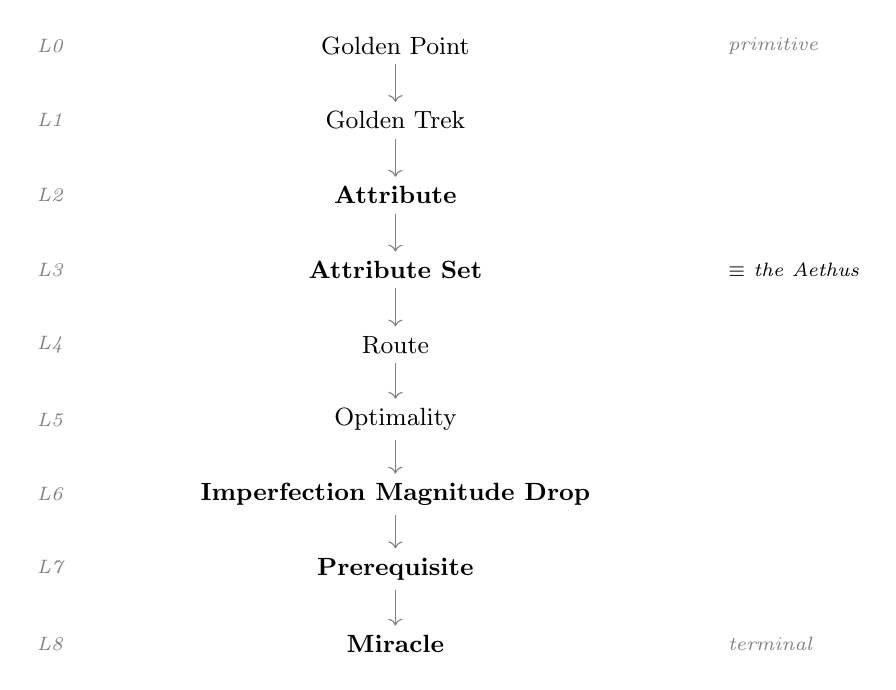
\begin{tikzpicture}[every node/.style={font=\small}]
  \node (n0) at (0,0)      {Golden Point};
  \node (n1) at (0,-0.95)  {Golden Trek};
  \node (n2) at (0,-1.90)  {\textbf{Attribute}};
  \node (n3) at (0,-2.85)  {\textbf{Attribute Set}};
  \node (n4) at (0,-3.80)  {Route};
  \node (n5) at (0,-4.75)  {Optimality};
  \node (n6) at (0,-5.70)  {\textbf{Imperfection Magnitude Drop}};
  \node (n7) at (0,-6.65)  {\textbf{Prerequisite}};
  \node (n8) at (0,-7.60)  {\textbf{Miracle}};
  \foreach \i/\j in {0/1,1/2,2/3,3/4,4/5,5/6,6/7,7/8}
      \draw[->, gray] (n\i) -- (n\j);
  \foreach \i in {0,...,8}
      \node[anchor=east, font=\scriptsize\itshape, gray] at (-4.1,-0.95*\i) {L\i};
  \node[anchor=west, font=\scriptsize\itshape] at (4.1,-2.85) {$\equiv$ the Aethus};
  \node[anchor=west, font=\scriptsize\itshape, gray] at (4.1,0) {primitive};
  \node[anchor=west, font=\scriptsize\itshape, gray] at (4.1,-7.60) {terminal};
\end{tikzpicture}
\caption{The spine of the late-2021 glossary: the longest derivation chain among its twenty-six terms, each defined using the one above it. Taking every definition as edges to the terms it invokes yields an acyclic graph of fifty-one edges resolving to just two primitives, of which \emph{Golden Point} is one; \emph{Miracle} sits alone at the far end as the system's terminal object, reached only after eight steps. Terms in bold survive into the present framework in name or in substance --- note that they are the upper reaches of the chain, the discarded scaffolding beneath them being precisely the teleological vocabulary of treks, routes and destinations. \emph{Attribute Set}, at the middle of the chain, is the Aethus under the name it was first given.}
\label{fig:2021-spine}
\end{figure}

One term deserves separate notice because it names something the present framework kept as an operation while dropping as a word. \emph{Auruman} designated ``an extension of the human species including all human ancestral organisms as part of the group,'' and \emph{Auruspective} the visualization of the past from within that group's experience. The convention of treating ancestral species as continuous with ourselves --- of writing ``us'' rather than ``them'' about Mesozoic mammals, which the Dark Era material depends on entirely and which the biosphere-level reading of Optimation formalizes --- is precisely Auruspectation without the name. The word was retired; the stance it named was not.

What the glossary establishes, then, is narrower and firmer than a claim about continuity of ideas. Six distinct operations of the mature framework --- the two weightings and their disagreement, the linkage scalar, its floor, the outward-insignificance restriction, the characterized null case, the perturbation-comparison over partial states, and the ancestral-continuity convention --- were all in hand as \emph{named} operations in late 2021, in a vocabulary that lacked every formal object the present paper uses to express them. That is the pre-formal operational content this section documents, attested by a contemporaneous dictionary rather than reconstructed from entries. And the teleological framing that the same document reveals is the counterweight: the developmental record shows a framework which had most of its operations early and spent the following years discovering that its own organizing metaphor was wrong.

\subsection{The 2022 Manuscript: Where Everything Sat, and What Was Not Yet Known}
\label{sec:manuscript-2022}
\label{sec:notational-provenance}

The glossary is the closing section of a longer document \cite{GoldenScience2022}, and the body of that document bears on a question the glossary alone cannot settle: not what the framework's operations were, but whether they were arrived at independently of the literature they now sit beside. The evidence there is notational, and notation is unusually good evidence, because it is the part of a piece of work that is hardest to acquire secondhand without acquiring the source along with it.

The relevant fact is that the 2022 manuscript states this paper's central constraint, and states it in letters of its own. Its Third Law of Auruspectation reads
\begin{equation*}
\frac{b}{a} \;<\; \frac{p}{1-p},
\end{equation*}
where $a$ is defined as the probability of eventual observers given that an attribute obtained, $b$ the same probability given that it did not, and $p$ the attribute's probability of occurrence in the set of all possibilities. Read against \autoref{prin:accordance}, that is the Accordance Principle: $a$ and $b$ are $\mathrm{P}(H \mid A)$ and $\mathrm{P}(H \mid A')$, so that $b/a$ is the canonical ratio, $p$ is $\mathrm{P}(A)$ under what the manuscript calls Outlook Probability and this paper calls the Cosmic Nexus, and the inequality is the same inequality. Its companion quantity is defined in the same section as
\begin{equation*}
L \;=\; \frac{a - b}{a + b},
\end{equation*}
which is existential linkage (\autoref{def:existential-linkage}) written out, and its \emph{L-Threshold} --- $L > 1 - 2p$ --- is the $\kappa = 1$ face of the linkage floor \eqref{eq:linkage-exceedance}, arrived at by algebraic rearrangement of the Third Law exactly as this paper derives it from the Accordance form.

What makes this worth recording is the choice of letters. Anyone reaching these results by way of the anthropic literature would have inherited that literature's notation with them, and would be writing conditional probabilities in the conditional-probability notation the field uses; the reasoning would arrive already dressed. The 2022 manuscript instead names the two observer-probabilities $a$ and $b$, the two weightings $p$ and $g$, the correlation $L$, and reaches the inequality through a route the literature does not take --- an argument about the proportion of observer ``mass'' distributed across timeline splits, generalizing the birth-index reasoning of the doomsday literature outward from positions in one history to positions across many. The result is the same result. The path to it is not a path the field had laid down.

The claim this supports should be stated at exactly its own strength and no more. The manuscript is not innocent of the literature: it cites the Rare Earth hypothesis, the Great Filter, the doomsday argument, and the Kardashev scale by name, and takes the first two as its explicit starting materials. What it lacks is any inheritance of the anthropic \emph{apparatus} --- no reference class formalism, no self-sampling or self-indication vocabulary, no observation-selection machinery, and no notation borrowed from any of them. The framework's own quantities were built from the mediocrity principle directly, and the correspondence between those quantities and this paper's is a correspondence between an independently constructed apparatus and its later formalization rather than between a source and a restatement.

Several of this paper's named results are recognizable there under the same description. The High Contrast Earth Hypothesis appears by that name, with the red dwarf construction and its cascade of compensating repairs already carrying the argument; the Second Law of Auruspectation states that an attribute statistically independent of the target has its two weightings coincide, which is the Theorem of Aimless Optimation (\autoref{sec:aimless}); outward insignificance is defined, together with the observation that the middle ground between it and high linkage is so hard to populate that finding a candidate there is itself evidence of insignificance --- the sharp binary of \autoref{sec:outwardly-insignificant}, stated as a working heuristic before it had a graph-theoretic argument behind it. The two-node dinosaurian derivation runs there in full, and the doomsday-pacing result appears in the same exponential form the present paper gives it. The differences are equally instructive, and one of them is worth making concrete, because it locates precisely what the intervening years had to supply. The manuscript contains a toy model --- a hypothetical trek which accumulates penalizing improbabilities at a constant hazard rate, each halving the probability of success --- and solves it exactly, finding that the observer-conditioned distribution over the number accumulated is $g(n) = 2^{-(n+1)}$: half of all successful treks pick up none, a quarter pick up one, and the tail falls geometrically. That is concentration on the optimum, in closed form and with nothing assumed. But it is concentration in the \emph{easy} case, and the reason is exactly the thing the model omits. Its severity classes carry no multiplicity: there is one way to accumulate $n$ penalties, so weight falls with severity and nothing pushes back. The whole difficulty of the sum-collapse (\autoref{lem:sum-collapse}) is that population does push back --- the cells at perturbation-depth $\Delta$ number $\binom{n}{\Delta}(b-1)^{\Delta}$ and grow faster than a per-attribute branching count would suggest --- so that the aggregate's fate turns on a race the toy never has to run. Read historically, then, the toy is not an early version of the collapse but a demonstration of the collapse's premise-free half, and the combinatorial half it does not contain is a fair summary of what remained to be done. Alongside it: the 2022 bounds are looser throughout, the premises are nowhere separated into assumptions and discharged conditions, and nothing is graded.


\subsubsection{A section-level concordance}
\label{sec:manuscript-concordance}

The provenance should be checkable at the grain of the document itself, and not only at the grain of ``the result appears there.'' The 2022 manuscript \cite{GoldenScience2022} runs to twenty-two numbered sections, and each of this paper's constructions sits in one of them. The table lists where. Two things it makes visible should be said first. The manuscript is not the beginning of formal Nexic reasoning---that is the 2021 record of \autoref{sec:aethic-connection}, the glossary of late 2021 being its closing section---but it is the last complete statement of the wing in its own pre-Aethic vocabulary, written across the very months in which the Aethic epiphany arrived (title page August 2022, the first version of the source; this version created November 2022), and so it is the fixed point against which every later formalization can be measured. And the concordance runs in both directions: everything in this paper traces to a section there, while several of the manuscript's sections trace to nothing here, having been superseded, absorbed, or set aside.

\begin{center}
\small
\begin{tabular}{@{}p{0.40\linewidth}p{0.55\linewidth}@{}}
\toprule
\emph{Golden Science} (2022), by section & Present paper \\
\midrule
§2 Invalidation of the Cosmological Mediocrity Principle & \autoref{sec:mediocrity-departures}: the arbitrariness of ``Earth-like planet'' as a reference class, now the departure from the received mediocrity principle \\
§3 Finding Prerequisites with the Mediocrity Principle & the two-node dinosaurian derivation, \autoref{prin:dinosaurian-probabilistic-context}, with the timeline-split ``mass'' argument as the route \\
§4 The Golden Point; the Golden Principle & the Golden reasoning paper's object, cited here by way of this manuscript \cite{GoldenScience2022}; its counterparts in the present paper are observer production $H$ and the astrobiological Copernican principle the Golden Principle stands against, \autoref{prin:astrobiological-copernican}. The ``Trace Connection'' the section leaves undefined is the question this paper hands to the Golden reasoning paper (\autoref{sec:situating-brief})---what the landed attribute was \emph{for}---and not anything settled here \\
§5 First Law of Auruspectation & the Copernican draw, \autoref{prin:copernican-draw}: the observer as a random element of the observer-producing histories; Outlook against Golden Probability is the Cosmic Nexus against the Aetherian Nexus, \autoref{nex:cosmic} and \autoref{nex:aetherian} \\
§6 Second Law of Auruspectation & the Theorem of Aimless Optimation, \autoref{prin:aimless-optimation}, posited there and proved here \\
§7 Third Law; the High Contrast Earth Hypothesis; Golden Linkage; outward insignificance & the Accordance Principle, \autoref{prin:accordance}; the HCEH, \autoref{sec:hceh}; existential linkage, \autoref{def:existential-linkage}; the outwardly-insignificant binary, \autoref{sec:outwardly-insignificant} \\
§8 Doomsday Pacing & \autoref{sec:pacing}, the same shortening bound and the same comparative static, now on competing-risks hardware \\
§9 Nescecoins & the toy model discussed above; superseded by the sum-collapse and its population term \\
§10 Hațeg Island; §11 Dark Era predation & the Dark Era, \autoref{sec:darkera}, with Hațeg as the safe-haven instance \\
§12 Temporal Third Law & the Third Law run over a duration; its worked bound, the theropod-dispersal argument for Hațeg, sits with the Dark Era treatment, \autoref{sec:darkera} \\
§13 Size constraints of the Chicxulub impactor & \autoref{sec:chicxulub-mass} \\
§14--15 Interstellar and interplanetary panspermia & \autoref{sec:panspermia} \\
§16 Difficulty Dynamics & set aside \\
§17 Task-Object & the Aethic paper's treatment \cite{Aethus}, alongside its July 2022 source \\
§18 Optimation & \autoref{sec:optimation}, the skewing of the Cosmic Nexus toward the Aetherian Nexus---the manuscript's own gloss, ``the act of skewing Outlook Probability to Golden Probability''---then defined as an act and now derived as a consequence \\
§19--20 Valuable Equations; Tournament Distribution & set aside \\
§22 Glossary & \autoref{sec:2021-glossary} \\
\bottomrule
\end{tabular}
\end{center}

\subsubsection{What was and was not known, and the reinvention of a conditional}
\label{sec:manuscript-epistemic-context}

The notational evidence of the preceding subsection bears on a stronger claim than independence from the anthropic apparatus, and the claim should be made because the manuscript supports it. When the Accordance Principle was constructed---before mid-2020, per \autoref{sec:accordance-origin}, and written into the form the manuscript states by 2021---its author had not yet learned conditional probability as a formal subject. The manuscript's letters are the evidence: $a$ and $b$ are ``the probability of humans evolving given that the dinosaurs are dead'' and ``given the definite survival of the dinosaurs,'' quantities that are conditional probabilities and that are nowhere written as such, because the notation $\mathrm{P}(\cdot \mid \cdot)$ and the definition behind it were not part of the equipment. The route to the inequality confirms it. The manuscript reaches $b/a < p/(1-p)$ not by conditioning but by counting: the total ``mass'' of observers is $p\,a + (1-p)\,b$, the proportion on the attribute's side is $p\,a/(p\,a + (1-p)\,b)$, and the mediocrity principle asks that proportion to exceed one half. That is a derivation of a conditional-probability inequality by someone constructing, from the mediocrity principle and a picture of observers distributed across timeline splits, the arithmetic that conditional probability would have supplied ready-made. The Aethic paper's observation that Bayesian reasoning is already Aethic-invariant---that inverting a conditional does not privilege the temporally earlier event, as Maxwell's equations were already relativistic before anyone knew to ask \cite{Aethus}---has its complement here: the Accordance Principle was built at the Aethic-invariant grade first, over classically complete timelines but with the tense-free structure already in it, by reinventing the relevant fragment of conditional probability rather than by applying it. The formal subject arrived afterward and was found to agree.

What the manuscript did know should be listed with the same care, so that the claim is not overstated. It cites the Rare Earth hypothesis and takes it as its starting material; it cites the Great Filter and works its dinosaurian example as one; it cites the doomsday argument and generalizes its birth-index reasoning outward from one history to many, which is the manuscript's own description of what it is doing; it cites the Kardashev scale in order to replace it. It does not know the anthropic literature's apparatus---no reference-class formalism, no self-sampling or self-indication assumption, no observation-selection theory---and it does not know the vocabulary of possible worlds or counterfactuals, its timeline splits and alternate realities being the layman's terms for what it later learned had names. Nor does it know that the constant external hazard it postulates in §8 is a competing-risks model with a standard treatment; it derives the exponential survival, the shortening bound, and the correct direction of the comparative static from the hazard function alone, and \autoref{sec:pacing} now records that the direction survived intact into the modern derivation while a later intermediate formulation briefly lost it. The pattern across all of these is one pattern: the manuscript is a document built from a small number of named starting points---the Rare Earth hypothesis, the mediocrity principle, the hazard function---by someone who did not have the intervening machinery and constructed, in each case, the part of it the problem required. That is the sense in which the provenance is seamless. Each result of this paper can be followed back to a section of a dated document, and the document can be seen not to have had the tools that would have made the results routine.

\subsection{Why the Axioms Became Theorems: Nexic Reasoning Rewritten on Aethic Hardware}
\label{sec:aethic-rewrite}
% NEXIC-TIER: ARCHIVE

The most conspicuous difference between the two framework generations is arithmetic. The 2022 manuscript carries three Laws of Auruspectation, each posited. The present paper carries one postulate --- the Copernican draw --- with the corresponding results derived from it. Reduction of that kind is easy to attribute to editorial maturation: a framework tidied, its overlaps merged, its statements economized. That attribution would be wrong, and the reason it is wrong is the substance of this subsection. The consolidation was not achieved by finding better proofs of the same statements within the same setting. It happened because the setting changed, and the statements that had to be posited in the old setting are consequences in the new one.

The defect is easiest to see in the old framework's most basic quantity. \emph{Outlook Probability} was defined as the probability of an attribute ``in the set of all possibilities'' --- deliberately indiscriminate, deliberately broad, and intended as the objective baseline against which the observer-weighted quantity would be compared. But read the phrase carefully and it carries a tense. The set of all possibilities \emph{as of when}? A probability of occurrence, quantified over possibilities, presupposes a vantage from which some things are settled and others open --- which is to say it presupposes a moving present, with determinacy behind it and possibility ahead. That presupposition has a name in the companion framework --- \emph{tensed determinacy}, the assumption that determinacy attaches to positions in time, so that an event's having occurred at an earlier moment thereby settles it for every later one \cite{Aethus}. The old framework never stated it, because in the timelike paradigm it is invisible: of course the past is fixed and the future is open, and of course probabilities are counted forward from now.

Aethic reasoning replaces tensed determinacy with observer-indexed determinacy, on which an outcome is determinate relative to an information state rather than to a position in time \cite{Aethus}. The decisive consequence is a single line --- \emph{blanks lack tense}: an unread attribute is blank whether its referent sits in the observer's past or future, and no vantage exists from which the settled and the open are globally distinguished. Outlook Probability, read against that ontology, is not merely imprecise; it is a category error --- it asks for a count over possibilities relative to a moment of pause that the ontology denies exists. This paper already records one symptom of the same defect: the difficulty, encountered in December 2021, of making the notion of a natural-historical \emph{Fluke} well-defined, since classifying an attribute as a fluke requires quantifying its probability of occurrence and there is no objective Aethus with which to reference it. That difficulty was not a local problem about flukes. It was the general defect in Outlook Probability, showing up first at the place where the quantification had to be made explicit.

The extrusion principle supplies the repair, and the repair is what forces the rest. With no causal timeline there is no Markovian preceding event from which probabilities may be counted forward, so probability must be indexed to a \emph{state} rather than to a moment --- an Aethus-within-Aethus weight per the relational weight principle, not a frequency taken from ``the time just before.'' A weighting over Aethae is precisely what this paper calls a Nexus. So the Nexus concept is not a generalization of Outlook Probability arrived at by abstraction; it is what Outlook Probability had to become once the vantage it presupposed was withdrawn.

Follow the consequences and the three Laws dissolve in order. The First Law --- consider oneself an element of a random Golden Trek among all Golden Treks --- had to be posited in the old setting, because it asserted a reference class that the timelike paradigm gave no standing to. Once states are the elemental objects, the reference class is not an assertion about how to reason but a description of what the objects are: the space of Aethae is the space of observer-situations, and nothing further needs stipulating. The Second Law --- statistical independence collapses the two weightings --- had to be posited because Outlook Probability and Golden Probability were separately defined quantities whose relationship was an open question. Once both are weightings over one class of object, differing only in their conditioning, their agreement on independent attributes is a fact about conditional probability, and the Theorem of Aimless Optimation (\autoref{sec:aimless}) proves it in three lines. And the Third Law --- the Accordance inequality itself --- had to be posited because in the old setting there was no law of realization to derive it from. Supply one, in the form of the Copernican draw over the children of a state, add the observer tilt, and the inequality follows by Bayes' theorem. What was an axiom becomes the conclusion of a two-line argument, not because the argument was cleverer but because there was finally something for it to argue from.

Grothendieck is the honest comparison here, and it is a comparison about method rather than magnitude. His formalisms came out cleaner not through ingenuity applied to existing objects but through replacement of the objects --- and the characteristic sign of that kind of progress is precisely this one: results that had to be assumed become results that follow, and separate results turn out to be one result seen from different sides. The cleanliness is downstream of a real ontological step, not of taste. The same holds here at a far smaller scale and with none of the same standing. Nexic reasoning was not tidied into its present shape; it was rewritten on different hardware, and the axiom count fell because the new substrate already contained what the old axioms had been compensating for.

Two honesties close the subsection. First, the rewrite did not eliminate assumption, it relocated it: the Copernican draw is a postulate, stated once and leaned on throughout, and a critic who rejects it rejects everything downstream --- the framework now has one exposed die-roll where it formerly had three, which is a gain in auditability and not a gain in certainty. Second, the direction of dependency this creates should be stated plainly rather than buried: because the consolidation is the Aethic ontology's doing, the present framework's economy is not independent evidence for it. A reader who declines tense-free blankness is entitled to regard the three-law formulation as the honest one, with the Nexus concept as an elegance purchased by an ontological commitment they have not granted. The corpus divides that labor deliberately: the ontology is argued in the companion \cite{Aethus}, and this paper's business is what follows once it is granted.
    
    \section{The Envelope Calibration of the Compounded Multiplier}
\label{app:nx-envelope}

\noindent This appendix keeps the first calibration of the many-attribute bound, as the record of how the bound was first priced. It bounds the compounded multiplier of Reading~1 through a stochastic envelope, needs observer-conditioned and draw-level independence, (I2) and (I3), and reaches the threshold $p < 1/(2\sqrt{e}) \approx 0.303$. The body uses the realized-cell bound, Lemma~\ref{lem:nx-realized-cell}, which needs neither condition and reaches $p < \tfrac12$; where the two differ, the body governs.

\textit{The compounded multiplier, in closed form.} Under Reading~1 the bound is a random quantity, and its distribution is available exactly once the draw's super-uniformity is used at the strength it actually has. That strength is the lower tail: $\Pr[Q_i < w] \le w$ for $w \le \tfrac12$, and nothing for $w > \tfrac12$, where a two-cell partition can put all its mass below $w$, (the derivation at the Copernican Draw above). In the variable $-\ln Q_i$ this reads $\Pr[-\ln Q_i > t] \le e^{-t}$ for $t \ge \ln 2$ and $\le 1$ for $t < \ln 2$, which is exactly the survival function of $\max(\ln 2,\, E_i)$ with $E_i \sim \mathrm{Exp}(1)$; the envelope is tight, the supremum over two-cell partitions attaining it at every $t$. So
\begin{equation}
\label{eq:domination-long}
-\ln Q_i \;\preceq_{\mathrm{st}}\; \max(\ln 2,\, E_i), \qquad E_i \sim \mathrm{Exp}(1),
\end{equation}
and not, as an earlier statement of this passage had it, $-\ln Q_i \preceq_{\mathrm{st}} \mathrm{Exp}(1)$, which would need the full super-uniformity the two-cell partition does not supply. The difference is a fair coin: an attribute of observer-conditioned weight $\tfrac12$ has $Q_i = \tfrac12$ with certainty and, by \eqref{eq:multiplier-identity}, $1 + \kappa_i = 2$ with certainty, a factor the exponential calibration put at its median but not its floor, and which each attribute in fact contributes at least. This is the one place (I3) is used, and it is used for exactly one thing: the joint law of the $Q_i$, which the pointwise factorization of (I2) does not supply. Stochastic dominance is preserved under sums of independent variables, so that \emph{under} {\rm (I3)},
\begin{equation}
\label{eq:gamma}
\ln \prod_{i=1}^{m} (1+\kappa_i) \;\preceq_{\mathrm{st}}\; \sum_{i=1}^{m} \max(\ln 2,\, E_i) \;=\; m \ln 2 \;+\; \Gamma(K, 1), \qquad K \sim \mathrm{Bin}(m, \tfrac12),
\end{equation}
the equality by memorylessness, each excess $(E_i - \ln 2)^{+}$ being zero with probability $\tfrac12$ and a fresh unit exponential otherwise. What follows is therefore the \emph{least favorable calibration} of the compounded multiplier and not its actual law; every bound read off it holds a fortiori for the true one, which is the sense in which the analysis is conservative at this step. The exceedance probability of the compounded multiplier follows in closed form:
\begin{equation}
\label{eq:multiplier-tail}
\Pr\!\left[\, \prod_{i=1}^{m}(1+\kappa_i) \;>\; t \,\right] \;\le\; \sum_{k=0}^{m} \binom{m}{k} 2^{-m}\, \Pr\!\big[\Gamma(k,1) > \ln t - m \ln 2\big], \qquad t \ge 2^{m},
\end{equation}
and $\le 1$ below $2^{m}$. At $m = 1$ and $t \ge 2$ the right-hand side is $1/t$, which is the Accordance tail $1/(1+\kappa)$ itself at $\kappa > 1$: the single-attribute principle is the $m = 1$ row of the compounded one, as it should be. Two consequences, and then the pipeline. \emph{First, the median.} The median of the envelope's compounded multiplier grows at the rate $\mathbb{E}[\max(\ln 2, E)] = \ln 2 + \tfrac12$ per attribute,
\begin{equation}
\label{eq:median-multiplier}
\ln \operatorname{med} \prod_{i=1}^{m} (1+\kappa_i) \;\approx\; \big(\ln 2 + \tfrac12\big)\, m \;\approx\; 1.19\, m,
\end{equation}
so compounding costs a factor of about $2\sqrt{e} \approx 3.3$ per attribute. This is the envelope's cost: the envelope's multiplier is heavy-tailed with infinite mean, the same non-integrability that forced the median reading of the tendency form at Corollary~\ref{cor:tendency}, appearing again where the same quantity is compounded, and it is the envelope's median that transports. The actual multiplier of a fixed binary partition is not heavy-tailed in this way. A side of observer-conditioned probability $q$ is realized with probability $q$ and contributes $1/q$, so its mean is exactly $2$ per attribute, and under draw-level independence Markov's inequality gives $\Pr\big[P(H^{+}) > (2p)^m/\delta\big] \le \delta$: the threshold $p < \tfrac12$, which the realized-cell bound of Lemma~\ref{lem:nx-realized-cell} reaches without that independence. \emph{Second, the threshold.} With each cosmic prior at $p$, the median bound of \eqref{eq:reading1} is
\begin{equation}
\label{eq:pe}
P(H^{+}) \;\lesssim\; \big(2\sqrt{e}\; p\big)^{m},
\end{equation}
which falls to zero as $m$ grows exactly when $2\sqrt{e}\,p < 1$, that is when
\[ p \;<\; \frac{1}{2\sqrt{e}} \;\approx\; 0.303 . \]
This is the threshold Reading~1 imposes, and it is worth stating as bluntly as it deserves, because it corrects an error the naive product invites. Thirty attributes at cosmic prior one half have a product of $2^{-30} \approx 10^{-9}$, which looks decisive; but their median compounded multiplier is about $2.4 \times 10^{15}$, so the bound is $P(H^{+}) \lesssim 2 \times 10^{6}$, which says nothing at all. The compounding outruns the product whenever $p > 0.303$. Thirty attributes at $p = 0.2$ give $\prod_i p_i \approx 1.1 \times 10^{-21}$ against a median multiplier of $2.4 \times 10^{15}$, hence $P(H^{+}) \lesssim 2.6 \times 10^{-6}$, which says a great deal; at $90\%$ confidence the multiplier is $1.9 \times 10^{18}$ and the bound $2 \times 10^{-3}$, at $95\%$ it is $1.7 \times 10^{-2}$, and at $99\%$ the multiplier $1.1 \times 10^{21}$ overtakes the product and the bound is vacuous. The difference between a vacuous bound and a decisive one is whether the priors clear $0.303$, and no amount of conjoining substitutes for that.\footnote{An earlier statement of this threshold was $p < 1/e \approx 0.368$, with a median multiplier of $e^{m - 1/3}$, derived from the exponential calibration that full super-uniformity would license. The two-cell correction moves the threshold to $0.303$ and the per-attribute cost from $e$ to $2\sqrt{e}$; every figure in this passage and in the extraction's multiplier table is recomputed accordingly.}

\textit{The pipeline.} The bound is evaluated on a record in four steps, and the steps are stated separately so that each can be audited on its own.
    \begin{enumerate}[label=(\arabic*), leftmargin=2.2em, itemsep=0.25em]
    \item \emph{List the attributes.} Enumerate $m$ realized attributes of the record whose cosmic priors are separately estimable from published work, and which are independent under the cosmic weighting. Record each $p_i$ with its source and its uncertainty. The independence claim is the one to argue explicitly; causal disconnection is the usual ground for it, and where two attributes share a common cause they are one attribute for this purpose.
    \item \emph{Choose a confidence.} Fix $\delta$, the probability with which the bound is permitted to fail. This is a choice of how much of the draw's tail to accept, not an estimate of anything.
    \item \emph{Read the multiplier.} Compute $t_\delta(m) = \exp\!\big(\Gamma^{-1}_{m,1}(1-\delta)\big)$, the $(1-\delta)$-quantile of the compounded multiplier, by inverting \eqref{eq:multiplier-tail} or from Table~\ref{tab:multiplier}.
    \item \emph{Report the bound.} $\Pr\big[P(H^{+}) > t_\delta(m)\prod_{i} p_i\big] \le \delta$, together with $m$, the list, and $\delta$, since the bound is uninterpretable without them.
    \end{enumerate}
    \begin{table}[htbp]
    \centering
    \caption{The compounded multiplier $t_\delta(m)$ of \eqref{eq:multiplier-tail}: with $m$ attributes independent under the cosmic weighting, $\Pr\big[P(H^{+}) > t_\delta(m)\prod_i p_i\big] \le \delta$. The $m=1$ row is the Accordance tail itself, $t_\delta(1) = 1/\delta$.}
    \label{tab:multiplier}
    \begin{tabular}{r rrrrr}
    \toprule
    $m$ & $\delta = 0.5$ & $0.25$ & $0.1$ & $0.05$ & $0.01$ \\
    \midrule
    1  & $2.0$ & $4.0$ & $10$ & $20$ & $100$ \\
    2  & $5.4$ & $15$ & $49$ & $115$ & $764$ \\
    3  & $14$ & $50$ & $205$ & $542$ & $4.5\times10^{3}$ \\
    5  & $107$ & $531$ & $2.96\times10^{3}$ & $9.45\times10^{3}$ & $1.10\times10^{5}$ \\
    10 & $1.58\times10^{4}$ & $1.49\times10^{5}$ & $1.48\times10^{6}$ & $6.62\times10^{6}$ & $1.44\times10^{8}$ \\
    20 & $3.48\times10^{8}$ & $8.04\times10^{9}$ & $1.78\times10^{11}$ & $1.28\times10^{12}$ & $6.77\times10^{13}$ \\
    30 & $7.66\times10^{12}$ & $3.51\times10^{14}$ & $1.43\times10^{16}$ & $1.49\times10^{17}$ & $1.55\times10^{19}$ \\
    \bottomrule
    \end{tabular}
    \end{table}

    \noindent

\emph{A worked case under the envelope, and how it degrades.} Take $m = 30$ attributes at cosmic prior $p = 0.2$ and a confidence of ninety percent. The product is $0.2^{30} \approx 1.1\times10^{-21}$; the table gives $t_{0.1}(30) \approx 1.4\times10^{16}$; the bound is $\Pr[P(H^{+}) > 1.6\times10^{-5}] \le 0.1$. At $p = 0.1$ the same thirty attributes give $1.4\times10^{-14}$. Now suppose a reader rejects six of the thirty---three whose priors they think overstated, three whose independence they doubt. The calculation moves to $m = 24$ and $\prod_i p_i = 0.2^{24}$, and can be redone from the table in a line; nothing else in the argument is touched. That is the separability Reading~1 was recommended for, and it is what makes the bound a claim a specialist can contest attribute by attribute rather than a claim they must accept or reject whole.
% R872 (Opus 5.5, Oct 27 2026), at the author's direction (the Pr[] form the default): the coverage bounds of this
% passage written in the exceedance form; they read "\le" with "at coverage $1-\delta$", "at confidence $1-\delta$" or
% "with probability at least" (Markov's bound, the pipeline's report, the table's caption, this case; R871 had the
% subscripted symbol).

\printbibliography
    
    \end{document}